\section{Methodology}

\subsection{Problem Statement}

To evaluate the impact of introducing a light rail network and park-and-ride (P\&R) facilities, we analyze road link usage under three scenarios:
\begin{description}
    \item[1. Base] No light rail is present; all trips are made by road.
    \item[2. Light Rail] The light rail can only be used if both the origin and destination are served by the network, with no transfers between modes allowed.
    \item[3. P\&R] The light rail can be used if either the origin or the destination is served by the network, representing the effect of park-and-ride facilities at stations.
\end{description}

We use the simplified Sioux Falls network as a case study. This network is widely used as a benchmark in traffic engineering due to its manageable size and typical grid structure, which allows for efficient computation and clear interpretation of results. Figure \ref{fig:casestudy} shows the road network and the origin-destination (OD) demand used in our analysis. The demand data is taken from the course assignment; while the exact units are not specified, we assume the values represent thousands of users.

\begin{figure}
    \centering
    \begin{subfigure}{0.5\textwidth}
        \centering
        \resizebox{\textwidth}{!}{%% Creator: Matplotlib, PGF backend
%%
%% To include the figure in your LaTeX document, write
%%   \input{<filename>.pgf}
%%
%% Make sure the required packages are loaded in your preamble
%%   \usepackage{pgf}
%%
%% Also ensure that all the required font packages are loaded; for instance,
%% the lmodern package is sometimes necessary when using math font.
%%   \usepackage{lmodern}
%%
%% Figures using additional raster images can only be included by \input if
%% they are in the same directory as the main LaTeX file. For loading figures
%% from other directories you can use the `import` package
%%   \usepackage{import}
%%
%% and then include the figures with
%%   \import{<path to file>}{<filename>.pgf}
%%
%% Matplotlib used the following preamble
%%   \def\mathdefault#1{#1}
%%   \everymath=\expandafter{\the\everymath\displaystyle}
%%   
%%   \ifdefined\pdftexversion\else  % non-pdftex case.
%%     \usepackage{fontspec}
%%     \setmainfont{DejaVuSerif.ttf}[Path=\detokenize{C:/Users/arsju/anaconda3/envs/Basic/Lib/site-packages/matplotlib/mpl-data/fonts/ttf/}]
%%     \setsansfont{DejaVuSans.ttf}[Path=\detokenize{C:/Users/arsju/anaconda3/envs/Basic/Lib/site-packages/matplotlib/mpl-data/fonts/ttf/}]
%%     \setmonofont{DejaVuSansMono.ttf}[Path=\detokenize{C:/Users/arsju/anaconda3/envs/Basic/Lib/site-packages/matplotlib/mpl-data/fonts/ttf/}]
%%   \fi
%%   \makeatletter\@ifpackageloaded{underscore}{}{\usepackage[strings]{underscore}}\makeatother
%%
\begingroup%
\makeatletter%
\begin{pgfpicture}%
\pgfpathrectangle{\pgfpointorigin}{\pgfqpoint{7.000000in}{7.000000in}}%
\pgfusepath{use as bounding box, clip}%
\begin{pgfscope}%
\pgfsetbuttcap%
\pgfsetmiterjoin%
\definecolor{currentfill}{rgb}{1.000000,1.000000,1.000000}%
\pgfsetfillcolor{currentfill}%
\pgfsetlinewidth{0.000000pt}%
\definecolor{currentstroke}{rgb}{1.000000,1.000000,1.000000}%
\pgfsetstrokecolor{currentstroke}%
\pgfsetdash{}{0pt}%
\pgfpathmoveto{\pgfqpoint{0.000000in}{0.000000in}}%
\pgfpathlineto{\pgfqpoint{7.000000in}{0.000000in}}%
\pgfpathlineto{\pgfqpoint{7.000000in}{7.000000in}}%
\pgfpathlineto{\pgfqpoint{0.000000in}{7.000000in}}%
\pgfpathlineto{\pgfqpoint{0.000000in}{0.000000in}}%
\pgfpathclose%
\pgfusepath{fill}%
\end{pgfscope}%
\begin{pgfscope}%
\pgfsetbuttcap%
\pgfsetmiterjoin%
\definecolor{currentfill}{rgb}{1.000000,1.000000,1.000000}%
\pgfsetfillcolor{currentfill}%
\pgfsetlinewidth{0.000000pt}%
\definecolor{currentstroke}{rgb}{0.000000,0.000000,0.000000}%
\pgfsetstrokecolor{currentstroke}%
\pgfsetstrokeopacity{0.000000}%
\pgfsetdash{}{0pt}%
\pgfpathmoveto{\pgfqpoint{1.419783in}{0.770000in}}%
\pgfpathlineto{\pgfqpoint{5.755217in}{0.770000in}}%
\pgfpathlineto{\pgfqpoint{5.755217in}{6.160000in}}%
\pgfpathlineto{\pgfqpoint{1.419783in}{6.160000in}}%
\pgfpathlineto{\pgfqpoint{1.419783in}{0.770000in}}%
\pgfpathclose%
\pgfusepath{fill}%
\end{pgfscope}%
\begin{pgfscope}%
\pgfpathrectangle{\pgfqpoint{1.419783in}{0.770000in}}{\pgfqpoint{4.335435in}{5.390000in}}%
\pgfusepath{clip}%
\pgfsetrectcap%
\pgfsetroundjoin%
\pgfsetlinewidth{1.003750pt}%
\definecolor{currentstroke}{rgb}{0.501961,0.501961,0.501961}%
\pgfsetstrokecolor{currentstroke}%
\pgfsetstrokeopacity{0.500000}%
\pgfsetdash{}{0pt}%
\pgfpathmoveto{\pgfqpoint{1.616848in}{5.915000in}}%
\pgfpathlineto{\pgfqpoint{4.492935in}{5.915000in}}%
\pgfusepath{stroke}%
\end{pgfscope}%
\begin{pgfscope}%
\pgfpathrectangle{\pgfqpoint{1.419783in}{0.770000in}}{\pgfqpoint{4.335435in}{5.390000in}}%
\pgfusepath{clip}%
\pgfsetrectcap%
\pgfsetroundjoin%
\pgfsetlinewidth{1.003750pt}%
\definecolor{currentstroke}{rgb}{0.501961,0.501961,0.501961}%
\pgfsetstrokecolor{currentstroke}%
\pgfsetstrokeopacity{0.500000}%
\pgfsetdash{}{0pt}%
\pgfpathmoveto{\pgfqpoint{1.616848in}{5.915000in}}%
\pgfpathlineto{\pgfqpoint{1.616848in}{5.169348in}}%
\pgfusepath{stroke}%
\end{pgfscope}%
\begin{pgfscope}%
\pgfpathrectangle{\pgfqpoint{1.419783in}{0.770000in}}{\pgfqpoint{4.335435in}{5.390000in}}%
\pgfusepath{clip}%
\pgfsetrectcap%
\pgfsetroundjoin%
\pgfsetlinewidth{1.003750pt}%
\definecolor{currentstroke}{rgb}{0.501961,0.501961,0.501961}%
\pgfsetstrokecolor{currentstroke}%
\pgfsetstrokeopacity{0.500000}%
\pgfsetdash{}{0pt}%
\pgfpathmoveto{\pgfqpoint{4.492935in}{5.915000in}}%
\pgfpathlineto{\pgfqpoint{1.616848in}{5.915000in}}%
\pgfusepath{stroke}%
\end{pgfscope}%
\begin{pgfscope}%
\pgfpathrectangle{\pgfqpoint{1.419783in}{0.770000in}}{\pgfqpoint{4.335435in}{5.390000in}}%
\pgfusepath{clip}%
\pgfsetrectcap%
\pgfsetroundjoin%
\pgfsetlinewidth{1.003750pt}%
\definecolor{currentstroke}{rgb}{0.501961,0.501961,0.501961}%
\pgfsetstrokecolor{currentstroke}%
\pgfsetstrokeopacity{0.500000}%
\pgfsetdash{}{0pt}%
\pgfpathmoveto{\pgfqpoint{4.492935in}{5.915000in}}%
\pgfpathlineto{\pgfqpoint{4.492935in}{5.169348in}}%
\pgfusepath{stroke}%
\end{pgfscope}%
\begin{pgfscope}%
\pgfpathrectangle{\pgfqpoint{1.419783in}{0.770000in}}{\pgfqpoint{4.335435in}{5.390000in}}%
\pgfusepath{clip}%
\pgfsetrectcap%
\pgfsetroundjoin%
\pgfsetlinewidth{1.003750pt}%
\definecolor{currentstroke}{rgb}{0.501961,0.501961,0.501961}%
\pgfsetstrokecolor{currentstroke}%
\pgfsetstrokeopacity{0.500000}%
\pgfsetdash{}{0pt}%
\pgfpathmoveto{\pgfqpoint{1.616848in}{5.169348in}}%
\pgfpathlineto{\pgfqpoint{1.616848in}{5.915000in}}%
\pgfusepath{stroke}%
\end{pgfscope}%
\begin{pgfscope}%
\pgfpathrectangle{\pgfqpoint{1.419783in}{0.770000in}}{\pgfqpoint{4.335435in}{5.390000in}}%
\pgfusepath{clip}%
\pgfsetrectcap%
\pgfsetroundjoin%
\pgfsetlinewidth{1.003750pt}%
\definecolor{currentstroke}{rgb}{0.501961,0.501961,0.501961}%
\pgfsetstrokecolor{currentstroke}%
\pgfsetstrokeopacity{0.500000}%
\pgfsetdash{}{0pt}%
\pgfpathmoveto{\pgfqpoint{1.616848in}{5.169348in}}%
\pgfpathlineto{\pgfqpoint{2.469022in}{5.169348in}}%
\pgfusepath{stroke}%
\end{pgfscope}%
\begin{pgfscope}%
\pgfpathrectangle{\pgfqpoint{1.419783in}{0.770000in}}{\pgfqpoint{4.335435in}{5.390000in}}%
\pgfusepath{clip}%
\pgfsetrectcap%
\pgfsetroundjoin%
\pgfsetlinewidth{1.003750pt}%
\definecolor{currentstroke}{rgb}{0.501961,0.501961,0.501961}%
\pgfsetstrokecolor{currentstroke}%
\pgfsetstrokeopacity{0.500000}%
\pgfsetdash{}{0pt}%
\pgfpathmoveto{\pgfqpoint{1.616848in}{5.169348in}}%
\pgfpathlineto{\pgfqpoint{1.616848in}{3.891087in}}%
\pgfusepath{stroke}%
\end{pgfscope}%
\begin{pgfscope}%
\pgfpathrectangle{\pgfqpoint{1.419783in}{0.770000in}}{\pgfqpoint{4.335435in}{5.390000in}}%
\pgfusepath{clip}%
\pgfsetrectcap%
\pgfsetroundjoin%
\pgfsetlinewidth{1.003750pt}%
\definecolor{currentstroke}{rgb}{0.501961,0.501961,0.501961}%
\pgfsetstrokecolor{currentstroke}%
\pgfsetstrokeopacity{0.500000}%
\pgfsetdash{}{0pt}%
\pgfpathmoveto{\pgfqpoint{2.469022in}{5.169348in}}%
\pgfpathlineto{\pgfqpoint{1.616848in}{5.169348in}}%
\pgfusepath{stroke}%
\end{pgfscope}%
\begin{pgfscope}%
\pgfpathrectangle{\pgfqpoint{1.419783in}{0.770000in}}{\pgfqpoint{4.335435in}{5.390000in}}%
\pgfusepath{clip}%
\pgfsetrectcap%
\pgfsetroundjoin%
\pgfsetlinewidth{1.003750pt}%
\definecolor{currentstroke}{rgb}{0.501961,0.501961,0.501961}%
\pgfsetstrokecolor{currentstroke}%
\pgfsetstrokeopacity{0.500000}%
\pgfsetdash{}{0pt}%
\pgfpathmoveto{\pgfqpoint{2.469022in}{5.169348in}}%
\pgfpathlineto{\pgfqpoint{3.427717in}{5.169348in}}%
\pgfusepath{stroke}%
\end{pgfscope}%
\begin{pgfscope}%
\pgfpathrectangle{\pgfqpoint{1.419783in}{0.770000in}}{\pgfqpoint{4.335435in}{5.390000in}}%
\pgfusepath{clip}%
\pgfsetrectcap%
\pgfsetroundjoin%
\pgfsetlinewidth{1.003750pt}%
\definecolor{currentstroke}{rgb}{0.501961,0.501961,0.501961}%
\pgfsetstrokecolor{currentstroke}%
\pgfsetstrokeopacity{0.500000}%
\pgfsetdash{}{0pt}%
\pgfpathmoveto{\pgfqpoint{2.469022in}{5.169348in}}%
\pgfpathlineto{\pgfqpoint{2.469022in}{3.891087in}}%
\pgfusepath{stroke}%
\end{pgfscope}%
\begin{pgfscope}%
\pgfpathrectangle{\pgfqpoint{1.419783in}{0.770000in}}{\pgfqpoint{4.335435in}{5.390000in}}%
\pgfusepath{clip}%
\pgfsetrectcap%
\pgfsetroundjoin%
\pgfsetlinewidth{1.003750pt}%
\definecolor{currentstroke}{rgb}{0.501961,0.501961,0.501961}%
\pgfsetstrokecolor{currentstroke}%
\pgfsetstrokeopacity{0.500000}%
\pgfsetdash{}{0pt}%
\pgfpathmoveto{\pgfqpoint{3.427717in}{5.169348in}}%
\pgfpathlineto{\pgfqpoint{2.469022in}{5.169348in}}%
\pgfusepath{stroke}%
\end{pgfscope}%
\begin{pgfscope}%
\pgfpathrectangle{\pgfqpoint{1.419783in}{0.770000in}}{\pgfqpoint{4.335435in}{5.390000in}}%
\pgfusepath{clip}%
\pgfsetrectcap%
\pgfsetroundjoin%
\pgfsetlinewidth{1.003750pt}%
\definecolor{currentstroke}{rgb}{0.501961,0.501961,0.501961}%
\pgfsetstrokecolor{currentstroke}%
\pgfsetstrokeopacity{0.500000}%
\pgfsetdash{}{0pt}%
\pgfpathmoveto{\pgfqpoint{3.427717in}{5.169348in}}%
\pgfpathlineto{\pgfqpoint{4.492935in}{5.169348in}}%
\pgfusepath{stroke}%
\end{pgfscope}%
\begin{pgfscope}%
\pgfpathrectangle{\pgfqpoint{1.419783in}{0.770000in}}{\pgfqpoint{4.335435in}{5.390000in}}%
\pgfusepath{clip}%
\pgfsetrectcap%
\pgfsetroundjoin%
\pgfsetlinewidth{1.003750pt}%
\definecolor{currentstroke}{rgb}{0.501961,0.501961,0.501961}%
\pgfsetstrokecolor{currentstroke}%
\pgfsetstrokeopacity{0.500000}%
\pgfsetdash{}{0pt}%
\pgfpathmoveto{\pgfqpoint{3.427717in}{5.169348in}}%
\pgfpathlineto{\pgfqpoint{3.427717in}{4.530217in}}%
\pgfusepath{stroke}%
\end{pgfscope}%
\begin{pgfscope}%
\pgfpathrectangle{\pgfqpoint{1.419783in}{0.770000in}}{\pgfqpoint{4.335435in}{5.390000in}}%
\pgfusepath{clip}%
\pgfsetrectcap%
\pgfsetroundjoin%
\pgfsetlinewidth{1.003750pt}%
\definecolor{currentstroke}{rgb}{0.501961,0.501961,0.501961}%
\pgfsetstrokecolor{currentstroke}%
\pgfsetstrokeopacity{0.500000}%
\pgfsetdash{}{0pt}%
\pgfpathmoveto{\pgfqpoint{4.492935in}{5.169348in}}%
\pgfpathlineto{\pgfqpoint{4.492935in}{5.915000in}}%
\pgfusepath{stroke}%
\end{pgfscope}%
\begin{pgfscope}%
\pgfpathrectangle{\pgfqpoint{1.419783in}{0.770000in}}{\pgfqpoint{4.335435in}{5.390000in}}%
\pgfusepath{clip}%
\pgfsetrectcap%
\pgfsetroundjoin%
\pgfsetlinewidth{1.003750pt}%
\definecolor{currentstroke}{rgb}{0.501961,0.501961,0.501961}%
\pgfsetstrokecolor{currentstroke}%
\pgfsetstrokeopacity{0.500000}%
\pgfsetdash{}{0pt}%
\pgfpathmoveto{\pgfqpoint{4.492935in}{5.169348in}}%
\pgfpathlineto{\pgfqpoint{3.427717in}{5.169348in}}%
\pgfusepath{stroke}%
\end{pgfscope}%
\begin{pgfscope}%
\pgfpathrectangle{\pgfqpoint{1.419783in}{0.770000in}}{\pgfqpoint{4.335435in}{5.390000in}}%
\pgfusepath{clip}%
\pgfsetrectcap%
\pgfsetroundjoin%
\pgfsetlinewidth{1.003750pt}%
\definecolor{currentstroke}{rgb}{0.501961,0.501961,0.501961}%
\pgfsetstrokecolor{currentstroke}%
\pgfsetstrokeopacity{0.500000}%
\pgfsetdash{}{0pt}%
\pgfpathmoveto{\pgfqpoint{4.492935in}{5.169348in}}%
\pgfpathlineto{\pgfqpoint{4.492935in}{4.530217in}}%
\pgfusepath{stroke}%
\end{pgfscope}%
\begin{pgfscope}%
\pgfpathrectangle{\pgfqpoint{1.419783in}{0.770000in}}{\pgfqpoint{4.335435in}{5.390000in}}%
\pgfusepath{clip}%
\pgfsetrectcap%
\pgfsetroundjoin%
\pgfsetlinewidth{1.003750pt}%
\definecolor{currentstroke}{rgb}{0.501961,0.501961,0.501961}%
\pgfsetstrokecolor{currentstroke}%
\pgfsetstrokeopacity{0.500000}%
\pgfsetdash{}{0pt}%
\pgfpathmoveto{\pgfqpoint{5.558152in}{4.530217in}}%
\pgfpathlineto{\pgfqpoint{4.492935in}{4.530217in}}%
\pgfusepath{stroke}%
\end{pgfscope}%
\begin{pgfscope}%
\pgfpathrectangle{\pgfqpoint{1.419783in}{0.770000in}}{\pgfqpoint{4.335435in}{5.390000in}}%
\pgfusepath{clip}%
\pgfsetrectcap%
\pgfsetroundjoin%
\pgfsetlinewidth{1.003750pt}%
\definecolor{currentstroke}{rgb}{0.501961,0.501961,0.501961}%
\pgfsetstrokecolor{currentstroke}%
\pgfsetstrokeopacity{0.500000}%
\pgfsetdash{}{0pt}%
\pgfpathmoveto{\pgfqpoint{5.558152in}{4.530217in}}%
\pgfpathlineto{\pgfqpoint{5.558152in}{3.891087in}}%
\pgfusepath{stroke}%
\end{pgfscope}%
\begin{pgfscope}%
\pgfpathrectangle{\pgfqpoint{1.419783in}{0.770000in}}{\pgfqpoint{4.335435in}{5.390000in}}%
\pgfusepath{clip}%
\pgfsetrectcap%
\pgfsetroundjoin%
\pgfsetlinewidth{1.003750pt}%
\definecolor{currentstroke}{rgb}{0.501961,0.501961,0.501961}%
\pgfsetstrokecolor{currentstroke}%
\pgfsetstrokeopacity{0.500000}%
\pgfsetdash{}{0pt}%
\pgfpathmoveto{\pgfqpoint{4.492935in}{4.530217in}}%
\pgfpathlineto{\pgfqpoint{4.492935in}{5.169348in}}%
\pgfusepath{stroke}%
\end{pgfscope}%
\begin{pgfscope}%
\pgfpathrectangle{\pgfqpoint{1.419783in}{0.770000in}}{\pgfqpoint{4.335435in}{5.390000in}}%
\pgfusepath{clip}%
\pgfsetrectcap%
\pgfsetroundjoin%
\pgfsetlinewidth{1.003750pt}%
\definecolor{currentstroke}{rgb}{0.501961,0.501961,0.501961}%
\pgfsetstrokecolor{currentstroke}%
\pgfsetstrokeopacity{0.500000}%
\pgfsetdash{}{0pt}%
\pgfpathmoveto{\pgfqpoint{4.492935in}{4.530217in}}%
\pgfpathlineto{\pgfqpoint{5.558152in}{4.530217in}}%
\pgfusepath{stroke}%
\end{pgfscope}%
\begin{pgfscope}%
\pgfpathrectangle{\pgfqpoint{1.419783in}{0.770000in}}{\pgfqpoint{4.335435in}{5.390000in}}%
\pgfusepath{clip}%
\pgfsetrectcap%
\pgfsetroundjoin%
\pgfsetlinewidth{1.003750pt}%
\definecolor{currentstroke}{rgb}{0.501961,0.501961,0.501961}%
\pgfsetstrokecolor{currentstroke}%
\pgfsetstrokeopacity{0.500000}%
\pgfsetdash{}{0pt}%
\pgfpathmoveto{\pgfqpoint{4.492935in}{4.530217in}}%
\pgfpathlineto{\pgfqpoint{3.427717in}{4.530217in}}%
\pgfusepath{stroke}%
\end{pgfscope}%
\begin{pgfscope}%
\pgfpathrectangle{\pgfqpoint{1.419783in}{0.770000in}}{\pgfqpoint{4.335435in}{5.390000in}}%
\pgfusepath{clip}%
\pgfsetrectcap%
\pgfsetroundjoin%
\pgfsetlinewidth{1.003750pt}%
\definecolor{currentstroke}{rgb}{0.501961,0.501961,0.501961}%
\pgfsetstrokecolor{currentstroke}%
\pgfsetstrokeopacity{0.500000}%
\pgfsetdash{}{0pt}%
\pgfpathmoveto{\pgfqpoint{4.492935in}{4.530217in}}%
\pgfpathlineto{\pgfqpoint{4.492935in}{3.891087in}}%
\pgfusepath{stroke}%
\end{pgfscope}%
\begin{pgfscope}%
\pgfpathrectangle{\pgfqpoint{1.419783in}{0.770000in}}{\pgfqpoint{4.335435in}{5.390000in}}%
\pgfusepath{clip}%
\pgfsetrectcap%
\pgfsetroundjoin%
\pgfsetlinewidth{1.003750pt}%
\definecolor{currentstroke}{rgb}{0.501961,0.501961,0.501961}%
\pgfsetstrokecolor{currentstroke}%
\pgfsetstrokeopacity{0.500000}%
\pgfsetdash{}{0pt}%
\pgfpathmoveto{\pgfqpoint{3.427717in}{4.530217in}}%
\pgfpathlineto{\pgfqpoint{3.427717in}{5.169348in}}%
\pgfusepath{stroke}%
\end{pgfscope}%
\begin{pgfscope}%
\pgfpathrectangle{\pgfqpoint{1.419783in}{0.770000in}}{\pgfqpoint{4.335435in}{5.390000in}}%
\pgfusepath{clip}%
\pgfsetrectcap%
\pgfsetroundjoin%
\pgfsetlinewidth{1.003750pt}%
\definecolor{currentstroke}{rgb}{0.501961,0.501961,0.501961}%
\pgfsetstrokecolor{currentstroke}%
\pgfsetstrokeopacity{0.500000}%
\pgfsetdash{}{0pt}%
\pgfpathmoveto{\pgfqpoint{3.427717in}{4.530217in}}%
\pgfpathlineto{\pgfqpoint{4.492935in}{4.530217in}}%
\pgfusepath{stroke}%
\end{pgfscope}%
\begin{pgfscope}%
\pgfpathrectangle{\pgfqpoint{1.419783in}{0.770000in}}{\pgfqpoint{4.335435in}{5.390000in}}%
\pgfusepath{clip}%
\pgfsetrectcap%
\pgfsetroundjoin%
\pgfsetlinewidth{1.003750pt}%
\definecolor{currentstroke}{rgb}{0.501961,0.501961,0.501961}%
\pgfsetstrokecolor{currentstroke}%
\pgfsetstrokeopacity{0.500000}%
\pgfsetdash{}{0pt}%
\pgfpathmoveto{\pgfqpoint{3.427717in}{4.530217in}}%
\pgfpathlineto{\pgfqpoint{3.427717in}{3.891087in}}%
\pgfusepath{stroke}%
\end{pgfscope}%
\begin{pgfscope}%
\pgfpathrectangle{\pgfqpoint{1.419783in}{0.770000in}}{\pgfqpoint{4.335435in}{5.390000in}}%
\pgfusepath{clip}%
\pgfsetrectcap%
\pgfsetroundjoin%
\pgfsetlinewidth{1.003750pt}%
\definecolor{currentstroke}{rgb}{0.501961,0.501961,0.501961}%
\pgfsetstrokecolor{currentstroke}%
\pgfsetstrokeopacity{0.500000}%
\pgfsetdash{}{0pt}%
\pgfpathmoveto{\pgfqpoint{3.427717in}{3.891087in}}%
\pgfpathlineto{\pgfqpoint{3.427717in}{4.530217in}}%
\pgfusepath{stroke}%
\end{pgfscope}%
\begin{pgfscope}%
\pgfpathrectangle{\pgfqpoint{1.419783in}{0.770000in}}{\pgfqpoint{4.335435in}{5.390000in}}%
\pgfusepath{clip}%
\pgfsetrectcap%
\pgfsetroundjoin%
\pgfsetlinewidth{1.003750pt}%
\definecolor{currentstroke}{rgb}{0.501961,0.501961,0.501961}%
\pgfsetstrokecolor{currentstroke}%
\pgfsetstrokeopacity{0.500000}%
\pgfsetdash{}{0pt}%
\pgfpathmoveto{\pgfqpoint{3.427717in}{3.891087in}}%
\pgfpathlineto{\pgfqpoint{2.469022in}{3.891087in}}%
\pgfusepath{stroke}%
\end{pgfscope}%
\begin{pgfscope}%
\pgfpathrectangle{\pgfqpoint{1.419783in}{0.770000in}}{\pgfqpoint{4.335435in}{5.390000in}}%
\pgfusepath{clip}%
\pgfsetrectcap%
\pgfsetroundjoin%
\pgfsetlinewidth{1.003750pt}%
\definecolor{currentstroke}{rgb}{0.501961,0.501961,0.501961}%
\pgfsetstrokecolor{currentstroke}%
\pgfsetstrokeopacity{0.500000}%
\pgfsetdash{}{0pt}%
\pgfpathmoveto{\pgfqpoint{3.427717in}{3.891087in}}%
\pgfpathlineto{\pgfqpoint{3.427717in}{2.506304in}}%
\pgfusepath{stroke}%
\end{pgfscope}%
\begin{pgfscope}%
\pgfpathrectangle{\pgfqpoint{1.419783in}{0.770000in}}{\pgfqpoint{4.335435in}{5.390000in}}%
\pgfusepath{clip}%
\pgfsetrectcap%
\pgfsetroundjoin%
\pgfsetlinewidth{1.003750pt}%
\definecolor{currentstroke}{rgb}{0.501961,0.501961,0.501961}%
\pgfsetstrokecolor{currentstroke}%
\pgfsetstrokeopacity{0.500000}%
\pgfsetdash{}{0pt}%
\pgfpathmoveto{\pgfqpoint{3.427717in}{3.891087in}}%
\pgfpathlineto{\pgfqpoint{4.492935in}{3.891087in}}%
\pgfusepath{stroke}%
\end{pgfscope}%
\begin{pgfscope}%
\pgfpathrectangle{\pgfqpoint{1.419783in}{0.770000in}}{\pgfqpoint{4.335435in}{5.390000in}}%
\pgfusepath{clip}%
\pgfsetrectcap%
\pgfsetroundjoin%
\pgfsetlinewidth{1.003750pt}%
\definecolor{currentstroke}{rgb}{0.501961,0.501961,0.501961}%
\pgfsetstrokecolor{currentstroke}%
\pgfsetstrokeopacity{0.500000}%
\pgfsetdash{}{0pt}%
\pgfpathmoveto{\pgfqpoint{3.427717in}{3.891087in}}%
\pgfpathlineto{\pgfqpoint{4.492935in}{3.251957in}}%
\pgfusepath{stroke}%
\end{pgfscope}%
\begin{pgfscope}%
\pgfpathrectangle{\pgfqpoint{1.419783in}{0.770000in}}{\pgfqpoint{4.335435in}{5.390000in}}%
\pgfusepath{clip}%
\pgfsetrectcap%
\pgfsetroundjoin%
\pgfsetlinewidth{1.003750pt}%
\definecolor{currentstroke}{rgb}{0.501961,0.501961,0.501961}%
\pgfsetstrokecolor{currentstroke}%
\pgfsetstrokeopacity{0.500000}%
\pgfsetdash{}{0pt}%
\pgfpathmoveto{\pgfqpoint{2.469022in}{3.891087in}}%
\pgfpathlineto{\pgfqpoint{2.469022in}{5.169348in}}%
\pgfusepath{stroke}%
\end{pgfscope}%
\begin{pgfscope}%
\pgfpathrectangle{\pgfqpoint{1.419783in}{0.770000in}}{\pgfqpoint{4.335435in}{5.390000in}}%
\pgfusepath{clip}%
\pgfsetrectcap%
\pgfsetroundjoin%
\pgfsetlinewidth{1.003750pt}%
\definecolor{currentstroke}{rgb}{0.501961,0.501961,0.501961}%
\pgfsetstrokecolor{currentstroke}%
\pgfsetstrokeopacity{0.500000}%
\pgfsetdash{}{0pt}%
\pgfpathmoveto{\pgfqpoint{2.469022in}{3.891087in}}%
\pgfpathlineto{\pgfqpoint{3.427717in}{3.891087in}}%
\pgfusepath{stroke}%
\end{pgfscope}%
\begin{pgfscope}%
\pgfpathrectangle{\pgfqpoint{1.419783in}{0.770000in}}{\pgfqpoint{4.335435in}{5.390000in}}%
\pgfusepath{clip}%
\pgfsetrectcap%
\pgfsetroundjoin%
\pgfsetlinewidth{1.003750pt}%
\definecolor{currentstroke}{rgb}{0.501961,0.501961,0.501961}%
\pgfsetstrokecolor{currentstroke}%
\pgfsetstrokeopacity{0.500000}%
\pgfsetdash{}{0pt}%
\pgfpathmoveto{\pgfqpoint{2.469022in}{3.891087in}}%
\pgfpathlineto{\pgfqpoint{1.616848in}{3.891087in}}%
\pgfusepath{stroke}%
\end{pgfscope}%
\begin{pgfscope}%
\pgfpathrectangle{\pgfqpoint{1.419783in}{0.770000in}}{\pgfqpoint{4.335435in}{5.390000in}}%
\pgfusepath{clip}%
\pgfsetrectcap%
\pgfsetroundjoin%
\pgfsetlinewidth{1.003750pt}%
\definecolor{currentstroke}{rgb}{0.501961,0.501961,0.501961}%
\pgfsetstrokecolor{currentstroke}%
\pgfsetstrokeopacity{0.500000}%
\pgfsetdash{}{0pt}%
\pgfpathmoveto{\pgfqpoint{2.469022in}{3.891087in}}%
\pgfpathlineto{\pgfqpoint{2.469022in}{2.506304in}}%
\pgfusepath{stroke}%
\end{pgfscope}%
\begin{pgfscope}%
\pgfpathrectangle{\pgfqpoint{1.419783in}{0.770000in}}{\pgfqpoint{4.335435in}{5.390000in}}%
\pgfusepath{clip}%
\pgfsetrectcap%
\pgfsetroundjoin%
\pgfsetlinewidth{1.003750pt}%
\definecolor{currentstroke}{rgb}{0.501961,0.501961,0.501961}%
\pgfsetstrokecolor{currentstroke}%
\pgfsetstrokeopacity{0.500000}%
\pgfsetdash{}{0pt}%
\pgfpathmoveto{\pgfqpoint{1.616848in}{3.891087in}}%
\pgfpathlineto{\pgfqpoint{1.616848in}{5.169348in}}%
\pgfusepath{stroke}%
\end{pgfscope}%
\begin{pgfscope}%
\pgfpathrectangle{\pgfqpoint{1.419783in}{0.770000in}}{\pgfqpoint{4.335435in}{5.390000in}}%
\pgfusepath{clip}%
\pgfsetrectcap%
\pgfsetroundjoin%
\pgfsetlinewidth{1.003750pt}%
\definecolor{currentstroke}{rgb}{0.501961,0.501961,0.501961}%
\pgfsetstrokecolor{currentstroke}%
\pgfsetstrokeopacity{0.500000}%
\pgfsetdash{}{0pt}%
\pgfpathmoveto{\pgfqpoint{1.616848in}{3.891087in}}%
\pgfpathlineto{\pgfqpoint{2.469022in}{3.891087in}}%
\pgfusepath{stroke}%
\end{pgfscope}%
\begin{pgfscope}%
\pgfpathrectangle{\pgfqpoint{1.419783in}{0.770000in}}{\pgfqpoint{4.335435in}{5.390000in}}%
\pgfusepath{clip}%
\pgfsetrectcap%
\pgfsetroundjoin%
\pgfsetlinewidth{1.003750pt}%
\definecolor{currentstroke}{rgb}{0.501961,0.501961,0.501961}%
\pgfsetstrokecolor{currentstroke}%
\pgfsetstrokeopacity{0.500000}%
\pgfsetdash{}{0pt}%
\pgfpathmoveto{\pgfqpoint{1.616848in}{3.891087in}}%
\pgfpathlineto{\pgfqpoint{1.616848in}{1.015000in}}%
\pgfusepath{stroke}%
\end{pgfscope}%
\begin{pgfscope}%
\pgfpathrectangle{\pgfqpoint{1.419783in}{0.770000in}}{\pgfqpoint{4.335435in}{5.390000in}}%
\pgfusepath{clip}%
\pgfsetrectcap%
\pgfsetroundjoin%
\pgfsetlinewidth{1.003750pt}%
\definecolor{currentstroke}{rgb}{0.501961,0.501961,0.501961}%
\pgfsetstrokecolor{currentstroke}%
\pgfsetstrokeopacity{0.500000}%
\pgfsetdash{}{0pt}%
\pgfpathmoveto{\pgfqpoint{1.616848in}{1.015000in}}%
\pgfpathlineto{\pgfqpoint{1.616848in}{3.891087in}}%
\pgfusepath{stroke}%
\end{pgfscope}%
\begin{pgfscope}%
\pgfpathrectangle{\pgfqpoint{1.419783in}{0.770000in}}{\pgfqpoint{4.335435in}{5.390000in}}%
\pgfusepath{clip}%
\pgfsetrectcap%
\pgfsetroundjoin%
\pgfsetlinewidth{1.003750pt}%
\definecolor{currentstroke}{rgb}{0.501961,0.501961,0.501961}%
\pgfsetstrokecolor{currentstroke}%
\pgfsetstrokeopacity{0.500000}%
\pgfsetdash{}{0pt}%
\pgfpathmoveto{\pgfqpoint{1.616848in}{1.015000in}}%
\pgfpathlineto{\pgfqpoint{2.469022in}{1.015000in}}%
\pgfusepath{stroke}%
\end{pgfscope}%
\begin{pgfscope}%
\pgfpathrectangle{\pgfqpoint{1.419783in}{0.770000in}}{\pgfqpoint{4.335435in}{5.390000in}}%
\pgfusepath{clip}%
\pgfsetrectcap%
\pgfsetroundjoin%
\pgfsetlinewidth{1.003750pt}%
\definecolor{currentstroke}{rgb}{0.501961,0.501961,0.501961}%
\pgfsetstrokecolor{currentstroke}%
\pgfsetstrokeopacity{0.500000}%
\pgfsetdash{}{0pt}%
\pgfpathmoveto{\pgfqpoint{2.469022in}{2.506304in}}%
\pgfpathlineto{\pgfqpoint{2.469022in}{3.891087in}}%
\pgfusepath{stroke}%
\end{pgfscope}%
\begin{pgfscope}%
\pgfpathrectangle{\pgfqpoint{1.419783in}{0.770000in}}{\pgfqpoint{4.335435in}{5.390000in}}%
\pgfusepath{clip}%
\pgfsetrectcap%
\pgfsetroundjoin%
\pgfsetlinewidth{1.003750pt}%
\definecolor{currentstroke}{rgb}{0.501961,0.501961,0.501961}%
\pgfsetstrokecolor{currentstroke}%
\pgfsetstrokeopacity{0.500000}%
\pgfsetdash{}{0pt}%
\pgfpathmoveto{\pgfqpoint{2.469022in}{2.506304in}}%
\pgfpathlineto{\pgfqpoint{3.427717in}{2.506304in}}%
\pgfusepath{stroke}%
\end{pgfscope}%
\begin{pgfscope}%
\pgfpathrectangle{\pgfqpoint{1.419783in}{0.770000in}}{\pgfqpoint{4.335435in}{5.390000in}}%
\pgfusepath{clip}%
\pgfsetrectcap%
\pgfsetroundjoin%
\pgfsetlinewidth{1.003750pt}%
\definecolor{currentstroke}{rgb}{0.501961,0.501961,0.501961}%
\pgfsetstrokecolor{currentstroke}%
\pgfsetstrokeopacity{0.500000}%
\pgfsetdash{}{0pt}%
\pgfpathmoveto{\pgfqpoint{2.469022in}{2.506304in}}%
\pgfpathlineto{\pgfqpoint{2.469022in}{1.867174in}}%
\pgfusepath{stroke}%
\end{pgfscope}%
\begin{pgfscope}%
\pgfpathrectangle{\pgfqpoint{1.419783in}{0.770000in}}{\pgfqpoint{4.335435in}{5.390000in}}%
\pgfusepath{clip}%
\pgfsetrectcap%
\pgfsetroundjoin%
\pgfsetlinewidth{1.003750pt}%
\definecolor{currentstroke}{rgb}{0.501961,0.501961,0.501961}%
\pgfsetstrokecolor{currentstroke}%
\pgfsetstrokeopacity{0.500000}%
\pgfsetdash{}{0pt}%
\pgfpathmoveto{\pgfqpoint{3.427717in}{2.506304in}}%
\pgfpathlineto{\pgfqpoint{3.427717in}{3.891087in}}%
\pgfusepath{stroke}%
\end{pgfscope}%
\begin{pgfscope}%
\pgfpathrectangle{\pgfqpoint{1.419783in}{0.770000in}}{\pgfqpoint{4.335435in}{5.390000in}}%
\pgfusepath{clip}%
\pgfsetrectcap%
\pgfsetroundjoin%
\pgfsetlinewidth{1.003750pt}%
\definecolor{currentstroke}{rgb}{0.501961,0.501961,0.501961}%
\pgfsetstrokecolor{currentstroke}%
\pgfsetstrokeopacity{0.500000}%
\pgfsetdash{}{0pt}%
\pgfpathmoveto{\pgfqpoint{3.427717in}{2.506304in}}%
\pgfpathlineto{\pgfqpoint{2.469022in}{2.506304in}}%
\pgfusepath{stroke}%
\end{pgfscope}%
\begin{pgfscope}%
\pgfpathrectangle{\pgfqpoint{1.419783in}{0.770000in}}{\pgfqpoint{4.335435in}{5.390000in}}%
\pgfusepath{clip}%
\pgfsetrectcap%
\pgfsetroundjoin%
\pgfsetlinewidth{1.003750pt}%
\definecolor{currentstroke}{rgb}{0.501961,0.501961,0.501961}%
\pgfsetstrokecolor{currentstroke}%
\pgfsetstrokeopacity{0.500000}%
\pgfsetdash{}{0pt}%
\pgfpathmoveto{\pgfqpoint{3.427717in}{2.506304in}}%
\pgfpathlineto{\pgfqpoint{4.492935in}{2.506304in}}%
\pgfusepath{stroke}%
\end{pgfscope}%
\begin{pgfscope}%
\pgfpathrectangle{\pgfqpoint{1.419783in}{0.770000in}}{\pgfqpoint{4.335435in}{5.390000in}}%
\pgfusepath{clip}%
\pgfsetrectcap%
\pgfsetroundjoin%
\pgfsetlinewidth{1.003750pt}%
\definecolor{currentstroke}{rgb}{0.501961,0.501961,0.501961}%
\pgfsetstrokecolor{currentstroke}%
\pgfsetstrokeopacity{0.500000}%
\pgfsetdash{}{0pt}%
\pgfpathmoveto{\pgfqpoint{3.427717in}{2.506304in}}%
\pgfpathlineto{\pgfqpoint{3.427717in}{1.867174in}}%
\pgfusepath{stroke}%
\end{pgfscope}%
\begin{pgfscope}%
\pgfpathrectangle{\pgfqpoint{1.419783in}{0.770000in}}{\pgfqpoint{4.335435in}{5.390000in}}%
\pgfusepath{clip}%
\pgfsetrectcap%
\pgfsetroundjoin%
\pgfsetlinewidth{1.003750pt}%
\definecolor{currentstroke}{rgb}{0.501961,0.501961,0.501961}%
\pgfsetstrokecolor{currentstroke}%
\pgfsetstrokeopacity{0.500000}%
\pgfsetdash{}{0pt}%
\pgfpathmoveto{\pgfqpoint{4.492935in}{3.891087in}}%
\pgfpathlineto{\pgfqpoint{4.492935in}{4.530217in}}%
\pgfusepath{stroke}%
\end{pgfscope}%
\begin{pgfscope}%
\pgfpathrectangle{\pgfqpoint{1.419783in}{0.770000in}}{\pgfqpoint{4.335435in}{5.390000in}}%
\pgfusepath{clip}%
\pgfsetrectcap%
\pgfsetroundjoin%
\pgfsetlinewidth{1.003750pt}%
\definecolor{currentstroke}{rgb}{0.501961,0.501961,0.501961}%
\pgfsetstrokecolor{currentstroke}%
\pgfsetstrokeopacity{0.500000}%
\pgfsetdash{}{0pt}%
\pgfpathmoveto{\pgfqpoint{4.492935in}{3.891087in}}%
\pgfpathlineto{\pgfqpoint{3.427717in}{3.891087in}}%
\pgfusepath{stroke}%
\end{pgfscope}%
\begin{pgfscope}%
\pgfpathrectangle{\pgfqpoint{1.419783in}{0.770000in}}{\pgfqpoint{4.335435in}{5.390000in}}%
\pgfusepath{clip}%
\pgfsetrectcap%
\pgfsetroundjoin%
\pgfsetlinewidth{1.003750pt}%
\definecolor{currentstroke}{rgb}{0.501961,0.501961,0.501961}%
\pgfsetstrokecolor{currentstroke}%
\pgfsetstrokeopacity{0.500000}%
\pgfsetdash{}{0pt}%
\pgfpathmoveto{\pgfqpoint{4.492935in}{3.891087in}}%
\pgfpathlineto{\pgfqpoint{4.492935in}{3.251957in}}%
\pgfusepath{stroke}%
\end{pgfscope}%
\begin{pgfscope}%
\pgfpathrectangle{\pgfqpoint{1.419783in}{0.770000in}}{\pgfqpoint{4.335435in}{5.390000in}}%
\pgfusepath{clip}%
\pgfsetrectcap%
\pgfsetroundjoin%
\pgfsetlinewidth{1.003750pt}%
\definecolor{currentstroke}{rgb}{0.501961,0.501961,0.501961}%
\pgfsetstrokecolor{currentstroke}%
\pgfsetstrokeopacity{0.500000}%
\pgfsetdash{}{0pt}%
\pgfpathmoveto{\pgfqpoint{4.492935in}{3.891087in}}%
\pgfpathlineto{\pgfqpoint{5.558152in}{3.891087in}}%
\pgfusepath{stroke}%
\end{pgfscope}%
\begin{pgfscope}%
\pgfpathrectangle{\pgfqpoint{1.419783in}{0.770000in}}{\pgfqpoint{4.335435in}{5.390000in}}%
\pgfusepath{clip}%
\pgfsetrectcap%
\pgfsetroundjoin%
\pgfsetlinewidth{1.003750pt}%
\definecolor{currentstroke}{rgb}{0.501961,0.501961,0.501961}%
\pgfsetstrokecolor{currentstroke}%
\pgfsetstrokeopacity{0.500000}%
\pgfsetdash{}{0pt}%
\pgfpathmoveto{\pgfqpoint{4.492935in}{3.251957in}}%
\pgfpathlineto{\pgfqpoint{3.427717in}{3.891087in}}%
\pgfusepath{stroke}%
\end{pgfscope}%
\begin{pgfscope}%
\pgfpathrectangle{\pgfqpoint{1.419783in}{0.770000in}}{\pgfqpoint{4.335435in}{5.390000in}}%
\pgfusepath{clip}%
\pgfsetrectcap%
\pgfsetroundjoin%
\pgfsetlinewidth{1.003750pt}%
\definecolor{currentstroke}{rgb}{0.501961,0.501961,0.501961}%
\pgfsetstrokecolor{currentstroke}%
\pgfsetstrokeopacity{0.500000}%
\pgfsetdash{}{0pt}%
\pgfpathmoveto{\pgfqpoint{4.492935in}{3.251957in}}%
\pgfpathlineto{\pgfqpoint{4.492935in}{3.891087in}}%
\pgfusepath{stroke}%
\end{pgfscope}%
\begin{pgfscope}%
\pgfpathrectangle{\pgfqpoint{1.419783in}{0.770000in}}{\pgfqpoint{4.335435in}{5.390000in}}%
\pgfusepath{clip}%
\pgfsetrectcap%
\pgfsetroundjoin%
\pgfsetlinewidth{1.003750pt}%
\definecolor{currentstroke}{rgb}{0.501961,0.501961,0.501961}%
\pgfsetstrokecolor{currentstroke}%
\pgfsetstrokeopacity{0.500000}%
\pgfsetdash{}{0pt}%
\pgfpathmoveto{\pgfqpoint{4.492935in}{3.251957in}}%
\pgfpathlineto{\pgfqpoint{4.492935in}{2.506304in}}%
\pgfusepath{stroke}%
\end{pgfscope}%
\begin{pgfscope}%
\pgfpathrectangle{\pgfqpoint{1.419783in}{0.770000in}}{\pgfqpoint{4.335435in}{5.390000in}}%
\pgfusepath{clip}%
\pgfsetrectcap%
\pgfsetroundjoin%
\pgfsetlinewidth{1.003750pt}%
\definecolor{currentstroke}{rgb}{0.501961,0.501961,0.501961}%
\pgfsetstrokecolor{currentstroke}%
\pgfsetstrokeopacity{0.500000}%
\pgfsetdash{}{0pt}%
\pgfpathmoveto{\pgfqpoint{5.558152in}{3.891087in}}%
\pgfpathlineto{\pgfqpoint{5.558152in}{4.530217in}}%
\pgfusepath{stroke}%
\end{pgfscope}%
\begin{pgfscope}%
\pgfpathrectangle{\pgfqpoint{1.419783in}{0.770000in}}{\pgfqpoint{4.335435in}{5.390000in}}%
\pgfusepath{clip}%
\pgfsetrectcap%
\pgfsetroundjoin%
\pgfsetlinewidth{1.003750pt}%
\definecolor{currentstroke}{rgb}{0.501961,0.501961,0.501961}%
\pgfsetstrokecolor{currentstroke}%
\pgfsetstrokeopacity{0.500000}%
\pgfsetdash{}{0pt}%
\pgfpathmoveto{\pgfqpoint{5.558152in}{3.891087in}}%
\pgfpathlineto{\pgfqpoint{4.492935in}{3.891087in}}%
\pgfusepath{stroke}%
\end{pgfscope}%
\begin{pgfscope}%
\pgfpathrectangle{\pgfqpoint{1.419783in}{0.770000in}}{\pgfqpoint{4.335435in}{5.390000in}}%
\pgfusepath{clip}%
\pgfsetrectcap%
\pgfsetroundjoin%
\pgfsetlinewidth{1.003750pt}%
\definecolor{currentstroke}{rgb}{0.501961,0.501961,0.501961}%
\pgfsetstrokecolor{currentstroke}%
\pgfsetstrokeopacity{0.500000}%
\pgfsetdash{}{0pt}%
\pgfpathmoveto{\pgfqpoint{5.558152in}{3.891087in}}%
\pgfpathlineto{\pgfqpoint{4.492935in}{1.015000in}}%
\pgfusepath{stroke}%
\end{pgfscope}%
\begin{pgfscope}%
\pgfpathrectangle{\pgfqpoint{1.419783in}{0.770000in}}{\pgfqpoint{4.335435in}{5.390000in}}%
\pgfusepath{clip}%
\pgfsetrectcap%
\pgfsetroundjoin%
\pgfsetlinewidth{1.003750pt}%
\definecolor{currentstroke}{rgb}{0.501961,0.501961,0.501961}%
\pgfsetstrokecolor{currentstroke}%
\pgfsetstrokeopacity{0.500000}%
\pgfsetdash{}{0pt}%
\pgfpathmoveto{\pgfqpoint{4.492935in}{2.506304in}}%
\pgfpathlineto{\pgfqpoint{3.427717in}{2.506304in}}%
\pgfusepath{stroke}%
\end{pgfscope}%
\begin{pgfscope}%
\pgfpathrectangle{\pgfqpoint{1.419783in}{0.770000in}}{\pgfqpoint{4.335435in}{5.390000in}}%
\pgfusepath{clip}%
\pgfsetrectcap%
\pgfsetroundjoin%
\pgfsetlinewidth{1.003750pt}%
\definecolor{currentstroke}{rgb}{0.501961,0.501961,0.501961}%
\pgfsetstrokecolor{currentstroke}%
\pgfsetstrokeopacity{0.500000}%
\pgfsetdash{}{0pt}%
\pgfpathmoveto{\pgfqpoint{4.492935in}{2.506304in}}%
\pgfpathlineto{\pgfqpoint{4.492935in}{3.251957in}}%
\pgfusepath{stroke}%
\end{pgfscope}%
\begin{pgfscope}%
\pgfpathrectangle{\pgfqpoint{1.419783in}{0.770000in}}{\pgfqpoint{4.335435in}{5.390000in}}%
\pgfusepath{clip}%
\pgfsetrectcap%
\pgfsetroundjoin%
\pgfsetlinewidth{1.003750pt}%
\definecolor{currentstroke}{rgb}{0.501961,0.501961,0.501961}%
\pgfsetstrokecolor{currentstroke}%
\pgfsetstrokeopacity{0.500000}%
\pgfsetdash{}{0pt}%
\pgfpathmoveto{\pgfqpoint{4.492935in}{2.506304in}}%
\pgfpathlineto{\pgfqpoint{4.492935in}{1.015000in}}%
\pgfusepath{stroke}%
\end{pgfscope}%
\begin{pgfscope}%
\pgfpathrectangle{\pgfqpoint{1.419783in}{0.770000in}}{\pgfqpoint{4.335435in}{5.390000in}}%
\pgfusepath{clip}%
\pgfsetrectcap%
\pgfsetroundjoin%
\pgfsetlinewidth{1.003750pt}%
\definecolor{currentstroke}{rgb}{0.501961,0.501961,0.501961}%
\pgfsetstrokecolor{currentstroke}%
\pgfsetstrokeopacity{0.500000}%
\pgfsetdash{}{0pt}%
\pgfpathmoveto{\pgfqpoint{4.492935in}{1.015000in}}%
\pgfpathlineto{\pgfqpoint{5.558152in}{3.891087in}}%
\pgfusepath{stroke}%
\end{pgfscope}%
\begin{pgfscope}%
\pgfpathrectangle{\pgfqpoint{1.419783in}{0.770000in}}{\pgfqpoint{4.335435in}{5.390000in}}%
\pgfusepath{clip}%
\pgfsetrectcap%
\pgfsetroundjoin%
\pgfsetlinewidth{1.003750pt}%
\definecolor{currentstroke}{rgb}{0.501961,0.501961,0.501961}%
\pgfsetstrokecolor{currentstroke}%
\pgfsetstrokeopacity{0.500000}%
\pgfsetdash{}{0pt}%
\pgfpathmoveto{\pgfqpoint{4.492935in}{1.015000in}}%
\pgfpathlineto{\pgfqpoint{4.492935in}{2.506304in}}%
\pgfusepath{stroke}%
\end{pgfscope}%
\begin{pgfscope}%
\pgfpathrectangle{\pgfqpoint{1.419783in}{0.770000in}}{\pgfqpoint{4.335435in}{5.390000in}}%
\pgfusepath{clip}%
\pgfsetrectcap%
\pgfsetroundjoin%
\pgfsetlinewidth{1.003750pt}%
\definecolor{currentstroke}{rgb}{0.501961,0.501961,0.501961}%
\pgfsetstrokecolor{currentstroke}%
\pgfsetstrokeopacity{0.500000}%
\pgfsetdash{}{0pt}%
\pgfpathmoveto{\pgfqpoint{4.492935in}{1.015000in}}%
\pgfpathlineto{\pgfqpoint{3.427717in}{1.015000in}}%
\pgfusepath{stroke}%
\end{pgfscope}%
\begin{pgfscope}%
\pgfpathrectangle{\pgfqpoint{1.419783in}{0.770000in}}{\pgfqpoint{4.335435in}{5.390000in}}%
\pgfusepath{clip}%
\pgfsetrectcap%
\pgfsetroundjoin%
\pgfsetlinewidth{1.003750pt}%
\definecolor{currentstroke}{rgb}{0.501961,0.501961,0.501961}%
\pgfsetstrokecolor{currentstroke}%
\pgfsetstrokeopacity{0.500000}%
\pgfsetdash{}{0pt}%
\pgfpathmoveto{\pgfqpoint{4.492935in}{1.015000in}}%
\pgfpathlineto{\pgfqpoint{3.427717in}{1.867174in}}%
\pgfusepath{stroke}%
\end{pgfscope}%
\begin{pgfscope}%
\pgfpathrectangle{\pgfqpoint{1.419783in}{0.770000in}}{\pgfqpoint{4.335435in}{5.390000in}}%
\pgfusepath{clip}%
\pgfsetrectcap%
\pgfsetroundjoin%
\pgfsetlinewidth{1.003750pt}%
\definecolor{currentstroke}{rgb}{0.501961,0.501961,0.501961}%
\pgfsetstrokecolor{currentstroke}%
\pgfsetstrokeopacity{0.500000}%
\pgfsetdash{}{0pt}%
\pgfpathmoveto{\pgfqpoint{3.427717in}{1.015000in}}%
\pgfpathlineto{\pgfqpoint{4.492935in}{1.015000in}}%
\pgfusepath{stroke}%
\end{pgfscope}%
\begin{pgfscope}%
\pgfpathrectangle{\pgfqpoint{1.419783in}{0.770000in}}{\pgfqpoint{4.335435in}{5.390000in}}%
\pgfusepath{clip}%
\pgfsetrectcap%
\pgfsetroundjoin%
\pgfsetlinewidth{1.003750pt}%
\definecolor{currentstroke}{rgb}{0.501961,0.501961,0.501961}%
\pgfsetstrokecolor{currentstroke}%
\pgfsetstrokeopacity{0.500000}%
\pgfsetdash{}{0pt}%
\pgfpathmoveto{\pgfqpoint{3.427717in}{1.015000in}}%
\pgfpathlineto{\pgfqpoint{3.427717in}{1.867174in}}%
\pgfusepath{stroke}%
\end{pgfscope}%
\begin{pgfscope}%
\pgfpathrectangle{\pgfqpoint{1.419783in}{0.770000in}}{\pgfqpoint{4.335435in}{5.390000in}}%
\pgfusepath{clip}%
\pgfsetrectcap%
\pgfsetroundjoin%
\pgfsetlinewidth{1.003750pt}%
\definecolor{currentstroke}{rgb}{0.501961,0.501961,0.501961}%
\pgfsetstrokecolor{currentstroke}%
\pgfsetstrokeopacity{0.500000}%
\pgfsetdash{}{0pt}%
\pgfpathmoveto{\pgfqpoint{3.427717in}{1.015000in}}%
\pgfpathlineto{\pgfqpoint{2.469022in}{1.015000in}}%
\pgfusepath{stroke}%
\end{pgfscope}%
\begin{pgfscope}%
\pgfpathrectangle{\pgfqpoint{1.419783in}{0.770000in}}{\pgfqpoint{4.335435in}{5.390000in}}%
\pgfusepath{clip}%
\pgfsetrectcap%
\pgfsetroundjoin%
\pgfsetlinewidth{1.003750pt}%
\definecolor{currentstroke}{rgb}{0.501961,0.501961,0.501961}%
\pgfsetstrokecolor{currentstroke}%
\pgfsetstrokeopacity{0.500000}%
\pgfsetdash{}{0pt}%
\pgfpathmoveto{\pgfqpoint{3.427717in}{1.867174in}}%
\pgfpathlineto{\pgfqpoint{3.427717in}{2.506304in}}%
\pgfusepath{stroke}%
\end{pgfscope}%
\begin{pgfscope}%
\pgfpathrectangle{\pgfqpoint{1.419783in}{0.770000in}}{\pgfqpoint{4.335435in}{5.390000in}}%
\pgfusepath{clip}%
\pgfsetrectcap%
\pgfsetroundjoin%
\pgfsetlinewidth{1.003750pt}%
\definecolor{currentstroke}{rgb}{0.501961,0.501961,0.501961}%
\pgfsetstrokecolor{currentstroke}%
\pgfsetstrokeopacity{0.500000}%
\pgfsetdash{}{0pt}%
\pgfpathmoveto{\pgfqpoint{3.427717in}{1.867174in}}%
\pgfpathlineto{\pgfqpoint{4.492935in}{1.015000in}}%
\pgfusepath{stroke}%
\end{pgfscope}%
\begin{pgfscope}%
\pgfpathrectangle{\pgfqpoint{1.419783in}{0.770000in}}{\pgfqpoint{4.335435in}{5.390000in}}%
\pgfusepath{clip}%
\pgfsetrectcap%
\pgfsetroundjoin%
\pgfsetlinewidth{1.003750pt}%
\definecolor{currentstroke}{rgb}{0.501961,0.501961,0.501961}%
\pgfsetstrokecolor{currentstroke}%
\pgfsetstrokeopacity{0.500000}%
\pgfsetdash{}{0pt}%
\pgfpathmoveto{\pgfqpoint{3.427717in}{1.867174in}}%
\pgfpathlineto{\pgfqpoint{3.427717in}{1.015000in}}%
\pgfusepath{stroke}%
\end{pgfscope}%
\begin{pgfscope}%
\pgfpathrectangle{\pgfqpoint{1.419783in}{0.770000in}}{\pgfqpoint{4.335435in}{5.390000in}}%
\pgfusepath{clip}%
\pgfsetrectcap%
\pgfsetroundjoin%
\pgfsetlinewidth{1.003750pt}%
\definecolor{currentstroke}{rgb}{0.501961,0.501961,0.501961}%
\pgfsetstrokecolor{currentstroke}%
\pgfsetstrokeopacity{0.500000}%
\pgfsetdash{}{0pt}%
\pgfpathmoveto{\pgfqpoint{3.427717in}{1.867174in}}%
\pgfpathlineto{\pgfqpoint{2.469022in}{1.867174in}}%
\pgfusepath{stroke}%
\end{pgfscope}%
\begin{pgfscope}%
\pgfpathrectangle{\pgfqpoint{1.419783in}{0.770000in}}{\pgfqpoint{4.335435in}{5.390000in}}%
\pgfusepath{clip}%
\pgfsetrectcap%
\pgfsetroundjoin%
\pgfsetlinewidth{1.003750pt}%
\definecolor{currentstroke}{rgb}{0.501961,0.501961,0.501961}%
\pgfsetstrokecolor{currentstroke}%
\pgfsetstrokeopacity{0.500000}%
\pgfsetdash{}{0pt}%
\pgfpathmoveto{\pgfqpoint{2.469022in}{1.867174in}}%
\pgfpathlineto{\pgfqpoint{2.469022in}{2.506304in}}%
\pgfusepath{stroke}%
\end{pgfscope}%
\begin{pgfscope}%
\pgfpathrectangle{\pgfqpoint{1.419783in}{0.770000in}}{\pgfqpoint{4.335435in}{5.390000in}}%
\pgfusepath{clip}%
\pgfsetrectcap%
\pgfsetroundjoin%
\pgfsetlinewidth{1.003750pt}%
\definecolor{currentstroke}{rgb}{0.501961,0.501961,0.501961}%
\pgfsetstrokecolor{currentstroke}%
\pgfsetstrokeopacity{0.500000}%
\pgfsetdash{}{0pt}%
\pgfpathmoveto{\pgfqpoint{2.469022in}{1.867174in}}%
\pgfpathlineto{\pgfqpoint{3.427717in}{1.867174in}}%
\pgfusepath{stroke}%
\end{pgfscope}%
\begin{pgfscope}%
\pgfpathrectangle{\pgfqpoint{1.419783in}{0.770000in}}{\pgfqpoint{4.335435in}{5.390000in}}%
\pgfusepath{clip}%
\pgfsetrectcap%
\pgfsetroundjoin%
\pgfsetlinewidth{1.003750pt}%
\definecolor{currentstroke}{rgb}{0.501961,0.501961,0.501961}%
\pgfsetstrokecolor{currentstroke}%
\pgfsetstrokeopacity{0.500000}%
\pgfsetdash{}{0pt}%
\pgfpathmoveto{\pgfqpoint{2.469022in}{1.867174in}}%
\pgfpathlineto{\pgfqpoint{2.469022in}{1.015000in}}%
\pgfusepath{stroke}%
\end{pgfscope}%
\begin{pgfscope}%
\pgfpathrectangle{\pgfqpoint{1.419783in}{0.770000in}}{\pgfqpoint{4.335435in}{5.390000in}}%
\pgfusepath{clip}%
\pgfsetrectcap%
\pgfsetroundjoin%
\pgfsetlinewidth{1.003750pt}%
\definecolor{currentstroke}{rgb}{0.501961,0.501961,0.501961}%
\pgfsetstrokecolor{currentstroke}%
\pgfsetstrokeopacity{0.500000}%
\pgfsetdash{}{0pt}%
\pgfpathmoveto{\pgfqpoint{2.469022in}{1.015000in}}%
\pgfpathlineto{\pgfqpoint{1.616848in}{1.015000in}}%
\pgfusepath{stroke}%
\end{pgfscope}%
\begin{pgfscope}%
\pgfpathrectangle{\pgfqpoint{1.419783in}{0.770000in}}{\pgfqpoint{4.335435in}{5.390000in}}%
\pgfusepath{clip}%
\pgfsetrectcap%
\pgfsetroundjoin%
\pgfsetlinewidth{1.003750pt}%
\definecolor{currentstroke}{rgb}{0.501961,0.501961,0.501961}%
\pgfsetstrokecolor{currentstroke}%
\pgfsetstrokeopacity{0.500000}%
\pgfsetdash{}{0pt}%
\pgfpathmoveto{\pgfqpoint{2.469022in}{1.015000in}}%
\pgfpathlineto{\pgfqpoint{3.427717in}{1.015000in}}%
\pgfusepath{stroke}%
\end{pgfscope}%
\begin{pgfscope}%
\pgfpathrectangle{\pgfqpoint{1.419783in}{0.770000in}}{\pgfqpoint{4.335435in}{5.390000in}}%
\pgfusepath{clip}%
\pgfsetrectcap%
\pgfsetroundjoin%
\pgfsetlinewidth{1.003750pt}%
\definecolor{currentstroke}{rgb}{0.501961,0.501961,0.501961}%
\pgfsetstrokecolor{currentstroke}%
\pgfsetstrokeopacity{0.500000}%
\pgfsetdash{}{0pt}%
\pgfpathmoveto{\pgfqpoint{2.469022in}{1.015000in}}%
\pgfpathlineto{\pgfqpoint{2.469022in}{1.867174in}}%
\pgfusepath{stroke}%
\end{pgfscope}%
\begin{pgfscope}%
\pgfsetrectcap%
\pgfsetmiterjoin%
\pgfsetlinewidth{0.803000pt}%
\definecolor{currentstroke}{rgb}{0.000000,0.000000,0.000000}%
\pgfsetstrokecolor{currentstroke}%
\pgfsetdash{}{0pt}%
\pgfpathmoveto{\pgfqpoint{1.419783in}{0.770000in}}%
\pgfpathlineto{\pgfqpoint{1.419783in}{6.160000in}}%
\pgfusepath{stroke}%
\end{pgfscope}%
\begin{pgfscope}%
\pgfsetrectcap%
\pgfsetmiterjoin%
\pgfsetlinewidth{0.803000pt}%
\definecolor{currentstroke}{rgb}{0.000000,0.000000,0.000000}%
\pgfsetstrokecolor{currentstroke}%
\pgfsetdash{}{0pt}%
\pgfpathmoveto{\pgfqpoint{5.755217in}{0.770000in}}%
\pgfpathlineto{\pgfqpoint{5.755217in}{6.160000in}}%
\pgfusepath{stroke}%
\end{pgfscope}%
\begin{pgfscope}%
\pgfsetrectcap%
\pgfsetmiterjoin%
\pgfsetlinewidth{0.803000pt}%
\definecolor{currentstroke}{rgb}{0.000000,0.000000,0.000000}%
\pgfsetstrokecolor{currentstroke}%
\pgfsetdash{}{0pt}%
\pgfpathmoveto{\pgfqpoint{1.419783in}{0.770000in}}%
\pgfpathlineto{\pgfqpoint{5.755217in}{0.770000in}}%
\pgfusepath{stroke}%
\end{pgfscope}%
\begin{pgfscope}%
\pgfsetrectcap%
\pgfsetmiterjoin%
\pgfsetlinewidth{0.803000pt}%
\definecolor{currentstroke}{rgb}{0.000000,0.000000,0.000000}%
\pgfsetstrokecolor{currentstroke}%
\pgfsetdash{}{0pt}%
\pgfpathmoveto{\pgfqpoint{1.419783in}{6.160000in}}%
\pgfpathlineto{\pgfqpoint{5.755217in}{6.160000in}}%
\pgfusepath{stroke}%
\end{pgfscope}%
\begin{pgfscope}%
\definecolor{textcolor}{rgb}{0.000000,0.000000,0.000000}%
\pgfsetstrokecolor{textcolor}%
\pgfsetfillcolor{textcolor}%
\pgftext[x=3.587500in,y=6.243333in,,base]{\color{textcolor}{\sffamily\fontsize{12.000000}{14.400000}\selectfont\catcode`\^=\active\def^{\ifmmode\sp\else\^{}\fi}\catcode`\%=\active\def%{\%}Network representation}}%
\end{pgfscope}%
\begin{pgfscope}%
\pgfsetbuttcap%
\pgfsetmiterjoin%
\definecolor{currentfill}{rgb}{1.000000,1.000000,1.000000}%
\pgfsetfillcolor{currentfill}%
\pgfsetfillopacity{0.800000}%
\pgfsetlinewidth{1.003750pt}%
\definecolor{currentstroke}{rgb}{0.800000,0.800000,0.800000}%
\pgfsetstrokecolor{currentstroke}%
\pgfsetstrokeopacity{0.800000}%
\pgfsetdash{}{0pt}%
\pgfpathmoveto{\pgfqpoint{4.405513in}{5.437317in}}%
\pgfpathlineto{\pgfqpoint{5.657995in}{5.437317in}}%
\pgfpathquadraticcurveto{\pgfqpoint{5.685773in}{5.437317in}}{\pgfqpoint{5.685773in}{5.465095in}}%
\pgfpathlineto{\pgfqpoint{5.685773in}{6.062778in}}%
\pgfpathquadraticcurveto{\pgfqpoint{5.685773in}{6.090556in}}{\pgfqpoint{5.657995in}{6.090556in}}%
\pgfpathlineto{\pgfqpoint{4.405513in}{6.090556in}}%
\pgfpathquadraticcurveto{\pgfqpoint{4.377735in}{6.090556in}}{\pgfqpoint{4.377735in}{6.062778in}}%
\pgfpathlineto{\pgfqpoint{4.377735in}{5.465095in}}%
\pgfpathquadraticcurveto{\pgfqpoint{4.377735in}{5.437317in}}{\pgfqpoint{4.405513in}{5.437317in}}%
\pgfpathlineto{\pgfqpoint{4.405513in}{5.437317in}}%
\pgfpathclose%
\pgfusepath{stroke,fill}%
\end{pgfscope}%
\begin{pgfscope}%
\pgfsetrectcap%
\pgfsetroundjoin%
\pgfsetlinewidth{1.003750pt}%
\definecolor{currentstroke}{rgb}{0.501961,0.501961,0.501961}%
\pgfsetstrokecolor{currentstroke}%
\pgfsetstrokeopacity{0.500000}%
\pgfsetdash{}{0pt}%
\pgfpathmoveto{\pgfqpoint{4.433291in}{5.978088in}}%
\pgfpathlineto{\pgfqpoint{4.572180in}{5.978088in}}%
\pgfpathlineto{\pgfqpoint{4.711069in}{5.978088in}}%
\pgfusepath{stroke}%
\end{pgfscope}%
\begin{pgfscope}%
\definecolor{textcolor}{rgb}{0.000000,0.000000,0.000000}%
\pgfsetstrokecolor{textcolor}%
\pgfsetfillcolor{textcolor}%
\pgftext[x=4.822180in,y=5.929477in,left,base]{\color{textcolor}{\sffamily\fontsize{10.000000}{12.000000}\selectfont\catcode`\^=\active\def^{\ifmmode\sp\else\^{}\fi}\catcode`\%=\active\def%{\%}Road links}}%
\end{pgfscope}%
\begin{pgfscope}%
\pgfsetrectcap%
\pgfsetroundjoin%
\pgfsetlinewidth{2.007500pt}%
\definecolor{currentstroke}{rgb}{1.000000,0.000000,0.000000}%
\pgfsetstrokecolor{currentstroke}%
\pgfsetdash{}{0pt}%
\pgfpathmoveto{\pgfqpoint{4.433291in}{5.774231in}}%
\pgfpathlineto{\pgfqpoint{4.572180in}{5.774231in}}%
\pgfpathlineto{\pgfqpoint{4.711069in}{5.774231in}}%
\pgfusepath{stroke}%
\end{pgfscope}%
\begin{pgfscope}%
\definecolor{textcolor}{rgb}{0.000000,0.000000,0.000000}%
\pgfsetstrokecolor{textcolor}%
\pgfsetfillcolor{textcolor}%
\pgftext[x=4.822180in,y=5.725620in,left,base]{\color{textcolor}{\sffamily\fontsize{10.000000}{12.000000}\selectfont\catcode`\^=\active\def^{\ifmmode\sp\else\^{}\fi}\catcode`\%=\active\def%{\%}Tram Line 1}}%
\end{pgfscope}%
\begin{pgfscope}%
\pgfsetrectcap%
\pgfsetroundjoin%
\pgfsetlinewidth{2.007500pt}%
\definecolor{currentstroke}{rgb}{1.000000,0.647059,0.000000}%
\pgfsetstrokecolor{currentstroke}%
\pgfsetdash{}{0pt}%
\pgfpathmoveto{\pgfqpoint{4.433291in}{5.570374in}}%
\pgfpathlineto{\pgfqpoint{4.572180in}{5.570374in}}%
\pgfpathlineto{\pgfqpoint{4.711069in}{5.570374in}}%
\pgfusepath{stroke}%
\end{pgfscope}%
\begin{pgfscope}%
\definecolor{textcolor}{rgb}{0.000000,0.000000,0.000000}%
\pgfsetstrokecolor{textcolor}%
\pgfsetfillcolor{textcolor}%
\pgftext[x=4.822180in,y=5.521762in,left,base]{\color{textcolor}{\sffamily\fontsize{10.000000}{12.000000}\selectfont\catcode`\^=\active\def^{\ifmmode\sp\else\^{}\fi}\catcode`\%=\active\def%{\%}Tram Line 2}}%
\end{pgfscope}%
\begin{pgfscope}%
\pgfpathrectangle{\pgfqpoint{1.419783in}{0.770000in}}{\pgfqpoint{4.335435in}{5.390000in}}%
\pgfusepath{clip}%
\pgfsetrectcap%
\pgfsetroundjoin%
\pgfsetlinewidth{2.007500pt}%
\definecolor{currentstroke}{rgb}{1.000000,0.000000,0.000000}%
\pgfsetstrokecolor{currentstroke}%
\pgfsetdash{}{0pt}%
\pgfpathmoveto{\pgfqpoint{1.616848in}{5.169348in}}%
\pgfpathlineto{\pgfqpoint{2.469022in}{5.169348in}}%
\pgfusepath{stroke}%
\end{pgfscope}%
\begin{pgfscope}%
\pgfpathrectangle{\pgfqpoint{1.419783in}{0.770000in}}{\pgfqpoint{4.335435in}{5.390000in}}%
\pgfusepath{clip}%
\pgfsetrectcap%
\pgfsetroundjoin%
\pgfsetlinewidth{2.007500pt}%
\definecolor{currentstroke}{rgb}{1.000000,0.000000,0.000000}%
\pgfsetstrokecolor{currentstroke}%
\pgfsetdash{}{0pt}%
\pgfpathmoveto{\pgfqpoint{2.469022in}{5.169348in}}%
\pgfpathlineto{\pgfqpoint{1.616848in}{5.169348in}}%
\pgfusepath{stroke}%
\end{pgfscope}%
\begin{pgfscope}%
\pgfpathrectangle{\pgfqpoint{1.419783in}{0.770000in}}{\pgfqpoint{4.335435in}{5.390000in}}%
\pgfusepath{clip}%
\pgfsetrectcap%
\pgfsetroundjoin%
\pgfsetlinewidth{2.007500pt}%
\definecolor{currentstroke}{rgb}{1.000000,0.000000,0.000000}%
\pgfsetstrokecolor{currentstroke}%
\pgfsetdash{}{0pt}%
\pgfpathmoveto{\pgfqpoint{2.469022in}{5.169348in}}%
\pgfpathlineto{\pgfqpoint{3.427717in}{5.169348in}}%
\pgfusepath{stroke}%
\end{pgfscope}%
\begin{pgfscope}%
\pgfpathrectangle{\pgfqpoint{1.419783in}{0.770000in}}{\pgfqpoint{4.335435in}{5.390000in}}%
\pgfusepath{clip}%
\pgfsetrectcap%
\pgfsetroundjoin%
\pgfsetlinewidth{2.007500pt}%
\definecolor{currentstroke}{rgb}{1.000000,0.000000,0.000000}%
\pgfsetstrokecolor{currentstroke}%
\pgfsetdash{}{0pt}%
\pgfpathmoveto{\pgfqpoint{3.427717in}{5.169348in}}%
\pgfpathlineto{\pgfqpoint{2.469022in}{5.169348in}}%
\pgfusepath{stroke}%
\end{pgfscope}%
\begin{pgfscope}%
\pgfpathrectangle{\pgfqpoint{1.419783in}{0.770000in}}{\pgfqpoint{4.335435in}{5.390000in}}%
\pgfusepath{clip}%
\pgfsetrectcap%
\pgfsetroundjoin%
\pgfsetlinewidth{2.007500pt}%
\definecolor{currentstroke}{rgb}{1.000000,0.000000,0.000000}%
\pgfsetstrokecolor{currentstroke}%
\pgfsetdash{}{0pt}%
\pgfpathmoveto{\pgfqpoint{3.427717in}{5.169348in}}%
\pgfpathlineto{\pgfqpoint{3.427717in}{4.530217in}}%
\pgfusepath{stroke}%
\end{pgfscope}%
\begin{pgfscope}%
\pgfpathrectangle{\pgfqpoint{1.419783in}{0.770000in}}{\pgfqpoint{4.335435in}{5.390000in}}%
\pgfusepath{clip}%
\pgfsetrectcap%
\pgfsetroundjoin%
\pgfsetlinewidth{2.007500pt}%
\definecolor{currentstroke}{rgb}{1.000000,0.000000,0.000000}%
\pgfsetstrokecolor{currentstroke}%
\pgfsetdash{}{0pt}%
\pgfpathmoveto{\pgfqpoint{3.427717in}{4.530217in}}%
\pgfpathlineto{\pgfqpoint{3.427717in}{5.169348in}}%
\pgfusepath{stroke}%
\end{pgfscope}%
\begin{pgfscope}%
\pgfpathrectangle{\pgfqpoint{1.419783in}{0.770000in}}{\pgfqpoint{4.335435in}{5.390000in}}%
\pgfusepath{clip}%
\pgfsetrectcap%
\pgfsetroundjoin%
\pgfsetlinewidth{2.007500pt}%
\definecolor{currentstroke}{rgb}{1.000000,0.000000,0.000000}%
\pgfsetstrokecolor{currentstroke}%
\pgfsetdash{}{0pt}%
\pgfpathmoveto{\pgfqpoint{3.427717in}{4.530217in}}%
\pgfpathlineto{\pgfqpoint{3.427717in}{3.891087in}}%
\pgfusepath{stroke}%
\end{pgfscope}%
\begin{pgfscope}%
\pgfpathrectangle{\pgfqpoint{1.419783in}{0.770000in}}{\pgfqpoint{4.335435in}{5.390000in}}%
\pgfusepath{clip}%
\pgfsetrectcap%
\pgfsetroundjoin%
\pgfsetlinewidth{2.007500pt}%
\definecolor{currentstroke}{rgb}{1.000000,0.000000,0.000000}%
\pgfsetstrokecolor{currentstroke}%
\pgfsetdash{}{0pt}%
\pgfpathmoveto{\pgfqpoint{3.427717in}{3.891087in}}%
\pgfpathlineto{\pgfqpoint{3.427717in}{4.530217in}}%
\pgfusepath{stroke}%
\end{pgfscope}%
\begin{pgfscope}%
\pgfpathrectangle{\pgfqpoint{1.419783in}{0.770000in}}{\pgfqpoint{4.335435in}{5.390000in}}%
\pgfusepath{clip}%
\pgfsetrectcap%
\pgfsetroundjoin%
\pgfsetlinewidth{2.007500pt}%
\definecolor{currentstroke}{rgb}{1.000000,0.000000,0.000000}%
\pgfsetstrokecolor{currentstroke}%
\pgfsetdash{}{0pt}%
\pgfpathmoveto{\pgfqpoint{3.427717in}{3.891087in}}%
\pgfpathlineto{\pgfqpoint{3.427717in}{2.506304in}}%
\pgfusepath{stroke}%
\end{pgfscope}%
\begin{pgfscope}%
\pgfpathrectangle{\pgfqpoint{1.419783in}{0.770000in}}{\pgfqpoint{4.335435in}{5.390000in}}%
\pgfusepath{clip}%
\pgfsetrectcap%
\pgfsetroundjoin%
\pgfsetlinewidth{2.007500pt}%
\definecolor{currentstroke}{rgb}{1.000000,0.000000,0.000000}%
\pgfsetstrokecolor{currentstroke}%
\pgfsetdash{}{0pt}%
\pgfpathmoveto{\pgfqpoint{3.427717in}{2.506304in}}%
\pgfpathlineto{\pgfqpoint{3.427717in}{3.891087in}}%
\pgfusepath{stroke}%
\end{pgfscope}%
\begin{pgfscope}%
\pgfpathrectangle{\pgfqpoint{1.419783in}{0.770000in}}{\pgfqpoint{4.335435in}{5.390000in}}%
\pgfusepath{clip}%
\pgfsetrectcap%
\pgfsetroundjoin%
\pgfsetlinewidth{2.007500pt}%
\definecolor{currentstroke}{rgb}{1.000000,0.000000,0.000000}%
\pgfsetstrokecolor{currentstroke}%
\pgfsetdash{}{0pt}%
\pgfpathmoveto{\pgfqpoint{3.427717in}{2.506304in}}%
\pgfpathlineto{\pgfqpoint{4.492935in}{2.506304in}}%
\pgfusepath{stroke}%
\end{pgfscope}%
\begin{pgfscope}%
\pgfpathrectangle{\pgfqpoint{1.419783in}{0.770000in}}{\pgfqpoint{4.335435in}{5.390000in}}%
\pgfusepath{clip}%
\pgfsetrectcap%
\pgfsetroundjoin%
\pgfsetlinewidth{2.007500pt}%
\definecolor{currentstroke}{rgb}{1.000000,0.000000,0.000000}%
\pgfsetstrokecolor{currentstroke}%
\pgfsetdash{}{0pt}%
\pgfpathmoveto{\pgfqpoint{4.492935in}{2.506304in}}%
\pgfpathlineto{\pgfqpoint{3.427717in}{2.506304in}}%
\pgfusepath{stroke}%
\end{pgfscope}%
\begin{pgfscope}%
\pgfpathrectangle{\pgfqpoint{1.419783in}{0.770000in}}{\pgfqpoint{4.335435in}{5.390000in}}%
\pgfusepath{clip}%
\pgfsetrectcap%
\pgfsetroundjoin%
\pgfsetlinewidth{2.007500pt}%
\definecolor{currentstroke}{rgb}{1.000000,0.647059,0.000000}%
\pgfsetstrokecolor{currentstroke}%
\pgfsetdash{}{0pt}%
\pgfpathmoveto{\pgfqpoint{1.616848in}{1.015000in}}%
\pgfpathlineto{\pgfqpoint{2.469022in}{1.015000in}}%
\pgfusepath{stroke}%
\end{pgfscope}%
\begin{pgfscope}%
\pgfpathrectangle{\pgfqpoint{1.419783in}{0.770000in}}{\pgfqpoint{4.335435in}{5.390000in}}%
\pgfusepath{clip}%
\pgfsetrectcap%
\pgfsetroundjoin%
\pgfsetlinewidth{2.007500pt}%
\definecolor{currentstroke}{rgb}{1.000000,0.647059,0.000000}%
\pgfsetstrokecolor{currentstroke}%
\pgfsetdash{}{0pt}%
\pgfpathmoveto{\pgfqpoint{2.469022in}{1.015000in}}%
\pgfpathlineto{\pgfqpoint{1.616848in}{1.015000in}}%
\pgfusepath{stroke}%
\end{pgfscope}%
\begin{pgfscope}%
\pgfpathrectangle{\pgfqpoint{1.419783in}{0.770000in}}{\pgfqpoint{4.335435in}{5.390000in}}%
\pgfusepath{clip}%
\pgfsetrectcap%
\pgfsetroundjoin%
\pgfsetlinewidth{2.007500pt}%
\definecolor{currentstroke}{rgb}{1.000000,0.647059,0.000000}%
\pgfsetstrokecolor{currentstroke}%
\pgfsetdash{}{0pt}%
\pgfpathmoveto{\pgfqpoint{2.469022in}{1.015000in}}%
\pgfpathlineto{\pgfqpoint{3.427717in}{1.015000in}}%
\pgfusepath{stroke}%
\end{pgfscope}%
\begin{pgfscope}%
\pgfpathrectangle{\pgfqpoint{1.419783in}{0.770000in}}{\pgfqpoint{4.335435in}{5.390000in}}%
\pgfusepath{clip}%
\pgfsetrectcap%
\pgfsetroundjoin%
\pgfsetlinewidth{2.007500pt}%
\definecolor{currentstroke}{rgb}{1.000000,0.647059,0.000000}%
\pgfsetstrokecolor{currentstroke}%
\pgfsetdash{}{0pt}%
\pgfpathmoveto{\pgfqpoint{3.427717in}{1.015000in}}%
\pgfpathlineto{\pgfqpoint{2.469022in}{1.015000in}}%
\pgfusepath{stroke}%
\end{pgfscope}%
\begin{pgfscope}%
\pgfpathrectangle{\pgfqpoint{1.419783in}{0.770000in}}{\pgfqpoint{4.335435in}{5.390000in}}%
\pgfusepath{clip}%
\pgfsetrectcap%
\pgfsetroundjoin%
\pgfsetlinewidth{2.007500pt}%
\definecolor{currentstroke}{rgb}{1.000000,0.647059,0.000000}%
\pgfsetstrokecolor{currentstroke}%
\pgfsetdash{}{0pt}%
\pgfpathmoveto{\pgfqpoint{3.427717in}{1.015000in}}%
\pgfpathlineto{\pgfqpoint{3.427717in}{1.867174in}}%
\pgfusepath{stroke}%
\end{pgfscope}%
\begin{pgfscope}%
\pgfpathrectangle{\pgfqpoint{1.419783in}{0.770000in}}{\pgfqpoint{4.335435in}{5.390000in}}%
\pgfusepath{clip}%
\pgfsetrectcap%
\pgfsetroundjoin%
\pgfsetlinewidth{2.007500pt}%
\definecolor{currentstroke}{rgb}{1.000000,0.647059,0.000000}%
\pgfsetstrokecolor{currentstroke}%
\pgfsetdash{}{0pt}%
\pgfpathmoveto{\pgfqpoint{3.427717in}{1.867174in}}%
\pgfpathlineto{\pgfqpoint{3.427717in}{1.015000in}}%
\pgfusepath{stroke}%
\end{pgfscope}%
\begin{pgfscope}%
\pgfpathrectangle{\pgfqpoint{1.419783in}{0.770000in}}{\pgfqpoint{4.335435in}{5.390000in}}%
\pgfusepath{clip}%
\pgfsetrectcap%
\pgfsetroundjoin%
\pgfsetlinewidth{2.007500pt}%
\definecolor{currentstroke}{rgb}{1.000000,0.647059,0.000000}%
\pgfsetstrokecolor{currentstroke}%
\pgfsetdash{}{0pt}%
\pgfpathmoveto{\pgfqpoint{3.427717in}{1.867174in}}%
\pgfpathlineto{\pgfqpoint{3.427717in}{2.506304in}}%
\pgfusepath{stroke}%
\end{pgfscope}%
\begin{pgfscope}%
\pgfpathrectangle{\pgfqpoint{1.419783in}{0.770000in}}{\pgfqpoint{4.335435in}{5.390000in}}%
\pgfusepath{clip}%
\pgfsetrectcap%
\pgfsetroundjoin%
\pgfsetlinewidth{2.007500pt}%
\definecolor{currentstroke}{rgb}{1.000000,0.647059,0.000000}%
\pgfsetstrokecolor{currentstroke}%
\pgfsetdash{}{0pt}%
\pgfpathmoveto{\pgfqpoint{3.427717in}{2.506304in}}%
\pgfpathlineto{\pgfqpoint{3.427717in}{1.867174in}}%
\pgfusepath{stroke}%
\end{pgfscope}%
\begin{pgfscope}%
\pgfpathrectangle{\pgfqpoint{1.419783in}{0.770000in}}{\pgfqpoint{4.335435in}{5.390000in}}%
\pgfusepath{clip}%
\pgfsetrectcap%
\pgfsetroundjoin%
\pgfsetlinewidth{2.007500pt}%
\definecolor{currentstroke}{rgb}{1.000000,0.647059,0.000000}%
\pgfsetstrokecolor{currentstroke}%
\pgfsetdash{}{0pt}%
\pgfpathmoveto{\pgfqpoint{3.427717in}{2.506304in}}%
\pgfpathlineto{\pgfqpoint{3.427717in}{3.891087in}}%
\pgfusepath{stroke}%
\end{pgfscope}%
\begin{pgfscope}%
\pgfpathrectangle{\pgfqpoint{1.419783in}{0.770000in}}{\pgfqpoint{4.335435in}{5.390000in}}%
\pgfusepath{clip}%
\pgfsetrectcap%
\pgfsetroundjoin%
\pgfsetlinewidth{2.007500pt}%
\definecolor{currentstroke}{rgb}{1.000000,0.647059,0.000000}%
\pgfsetstrokecolor{currentstroke}%
\pgfsetdash{}{0pt}%
\pgfpathmoveto{\pgfqpoint{3.427717in}{3.891087in}}%
\pgfpathlineto{\pgfqpoint{3.427717in}{2.506304in}}%
\pgfusepath{stroke}%
\end{pgfscope}%
\begin{pgfscope}%
\pgfpathrectangle{\pgfqpoint{1.419783in}{0.770000in}}{\pgfqpoint{4.335435in}{5.390000in}}%
\pgfusepath{clip}%
\pgfsetrectcap%
\pgfsetroundjoin%
\pgfsetlinewidth{2.007500pt}%
\definecolor{currentstroke}{rgb}{1.000000,0.647059,0.000000}%
\pgfsetstrokecolor{currentstroke}%
\pgfsetdash{}{0pt}%
\pgfpathmoveto{\pgfqpoint{3.427717in}{3.891087in}}%
\pgfpathlineto{\pgfqpoint{4.492935in}{3.891087in}}%
\pgfusepath{stroke}%
\end{pgfscope}%
\begin{pgfscope}%
\pgfpathrectangle{\pgfqpoint{1.419783in}{0.770000in}}{\pgfqpoint{4.335435in}{5.390000in}}%
\pgfusepath{clip}%
\pgfsetrectcap%
\pgfsetroundjoin%
\pgfsetlinewidth{2.007500pt}%
\definecolor{currentstroke}{rgb}{1.000000,0.647059,0.000000}%
\pgfsetstrokecolor{currentstroke}%
\pgfsetdash{}{0pt}%
\pgfpathmoveto{\pgfqpoint{4.492935in}{3.891087in}}%
\pgfpathlineto{\pgfqpoint{3.427717in}{3.891087in}}%
\pgfusepath{stroke}%
\end{pgfscope}%
\begin{pgfscope}%
\pgfpathrectangle{\pgfqpoint{1.419783in}{0.770000in}}{\pgfqpoint{4.335435in}{5.390000in}}%
\pgfusepath{clip}%
\pgfsetrectcap%
\pgfsetroundjoin%
\pgfsetlinewidth{2.007500pt}%
\definecolor{currentstroke}{rgb}{1.000000,0.647059,0.000000}%
\pgfsetstrokecolor{currentstroke}%
\pgfsetdash{}{0pt}%
\pgfpathmoveto{\pgfqpoint{4.492935in}{3.891087in}}%
\pgfpathlineto{\pgfqpoint{4.492935in}{4.530217in}}%
\pgfusepath{stroke}%
\end{pgfscope}%
\begin{pgfscope}%
\pgfpathrectangle{\pgfqpoint{1.419783in}{0.770000in}}{\pgfqpoint{4.335435in}{5.390000in}}%
\pgfusepath{clip}%
\pgfsetrectcap%
\pgfsetroundjoin%
\pgfsetlinewidth{2.007500pt}%
\definecolor{currentstroke}{rgb}{1.000000,0.647059,0.000000}%
\pgfsetstrokecolor{currentstroke}%
\pgfsetdash{}{0pt}%
\pgfpathmoveto{\pgfqpoint{4.492935in}{4.530217in}}%
\pgfpathlineto{\pgfqpoint{4.492935in}{3.891087in}}%
\pgfusepath{stroke}%
\end{pgfscope}%
\begin{pgfscope}%
\pgfpathrectangle{\pgfqpoint{1.419783in}{0.770000in}}{\pgfqpoint{4.335435in}{5.390000in}}%
\pgfusepath{clip}%
\pgfsetrectcap%
\pgfsetroundjoin%
\pgfsetlinewidth{2.007500pt}%
\definecolor{currentstroke}{rgb}{1.000000,0.647059,0.000000}%
\pgfsetstrokecolor{currentstroke}%
\pgfsetdash{}{0pt}%
\pgfpathmoveto{\pgfqpoint{4.492935in}{4.530217in}}%
\pgfpathlineto{\pgfqpoint{4.492935in}{5.169348in}}%
\pgfusepath{stroke}%
\end{pgfscope}%
\begin{pgfscope}%
\pgfpathrectangle{\pgfqpoint{1.419783in}{0.770000in}}{\pgfqpoint{4.335435in}{5.390000in}}%
\pgfusepath{clip}%
\pgfsetrectcap%
\pgfsetroundjoin%
\pgfsetlinewidth{2.007500pt}%
\definecolor{currentstroke}{rgb}{1.000000,0.647059,0.000000}%
\pgfsetstrokecolor{currentstroke}%
\pgfsetdash{}{0pt}%
\pgfpathmoveto{\pgfqpoint{4.492935in}{5.169348in}}%
\pgfpathlineto{\pgfqpoint{4.492935in}{4.530217in}}%
\pgfusepath{stroke}%
\end{pgfscope}%
\begin{pgfscope}%
\pgfpathrectangle{\pgfqpoint{1.419783in}{0.770000in}}{\pgfqpoint{4.335435in}{5.390000in}}%
\pgfusepath{clip}%
\pgfsetbuttcap%
\pgfsetroundjoin%
\definecolor{currentfill}{rgb}{0.000000,0.000000,1.000000}%
\pgfsetfillcolor{currentfill}%
\pgfsetlinewidth{1.003750pt}%
\definecolor{currentstroke}{rgb}{0.000000,0.000000,1.000000}%
\pgfsetstrokecolor{currentstroke}%
\pgfsetdash{}{0pt}%
\pgfsys@defobject{currentmarker}{\pgfqpoint{-0.069444in}{-0.069444in}}{\pgfqpoint{0.069444in}{0.069444in}}{%
\pgfpathmoveto{\pgfqpoint{0.000000in}{-0.069444in}}%
\pgfpathcurveto{\pgfqpoint{0.018417in}{-0.069444in}}{\pgfqpoint{0.036082in}{-0.062127in}}{\pgfqpoint{0.049105in}{-0.049105in}}%
\pgfpathcurveto{\pgfqpoint{0.062127in}{-0.036082in}}{\pgfqpoint{0.069444in}{-0.018417in}}{\pgfqpoint{0.069444in}{0.000000in}}%
\pgfpathcurveto{\pgfqpoint{0.069444in}{0.018417in}}{\pgfqpoint{0.062127in}{0.036082in}}{\pgfqpoint{0.049105in}{0.049105in}}%
\pgfpathcurveto{\pgfqpoint{0.036082in}{0.062127in}}{\pgfqpoint{0.018417in}{0.069444in}}{\pgfqpoint{0.000000in}{0.069444in}}%
\pgfpathcurveto{\pgfqpoint{-0.018417in}{0.069444in}}{\pgfqpoint{-0.036082in}{0.062127in}}{\pgfqpoint{-0.049105in}{0.049105in}}%
\pgfpathcurveto{\pgfqpoint{-0.062127in}{0.036082in}}{\pgfqpoint{-0.069444in}{0.018417in}}{\pgfqpoint{-0.069444in}{0.000000in}}%
\pgfpathcurveto{\pgfqpoint{-0.069444in}{-0.018417in}}{\pgfqpoint{-0.062127in}{-0.036082in}}{\pgfqpoint{-0.049105in}{-0.049105in}}%
\pgfpathcurveto{\pgfqpoint{-0.036082in}{-0.062127in}}{\pgfqpoint{-0.018417in}{-0.069444in}}{\pgfqpoint{0.000000in}{-0.069444in}}%
\pgfpathlineto{\pgfqpoint{0.000000in}{-0.069444in}}%
\pgfpathclose%
\pgfusepath{stroke,fill}%
}%
\begin{pgfscope}%
\pgfsys@transformshift{1.616848in}{5.915000in}%
\pgfsys@useobject{currentmarker}{}%
\end{pgfscope}%
\begin{pgfscope}%
\pgfsys@transformshift{4.492935in}{5.915000in}%
\pgfsys@useobject{currentmarker}{}%
\end{pgfscope}%
\begin{pgfscope}%
\pgfsys@transformshift{1.616848in}{5.169348in}%
\pgfsys@useobject{currentmarker}{}%
\end{pgfscope}%
\begin{pgfscope}%
\pgfsys@transformshift{2.469022in}{5.169348in}%
\pgfsys@useobject{currentmarker}{}%
\end{pgfscope}%
\begin{pgfscope}%
\pgfsys@transformshift{3.427717in}{5.169348in}%
\pgfsys@useobject{currentmarker}{}%
\end{pgfscope}%
\begin{pgfscope}%
\pgfsys@transformshift{4.492935in}{5.169348in}%
\pgfsys@useobject{currentmarker}{}%
\end{pgfscope}%
\begin{pgfscope}%
\pgfsys@transformshift{5.558152in}{4.530217in}%
\pgfsys@useobject{currentmarker}{}%
\end{pgfscope}%
\begin{pgfscope}%
\pgfsys@transformshift{4.492935in}{4.530217in}%
\pgfsys@useobject{currentmarker}{}%
\end{pgfscope}%
\begin{pgfscope}%
\pgfsys@transformshift{3.427717in}{4.530217in}%
\pgfsys@useobject{currentmarker}{}%
\end{pgfscope}%
\begin{pgfscope}%
\pgfsys@transformshift{3.427717in}{3.891087in}%
\pgfsys@useobject{currentmarker}{}%
\end{pgfscope}%
\begin{pgfscope}%
\pgfsys@transformshift{2.469022in}{3.891087in}%
\pgfsys@useobject{currentmarker}{}%
\end{pgfscope}%
\begin{pgfscope}%
\pgfsys@transformshift{1.616848in}{3.891087in}%
\pgfsys@useobject{currentmarker}{}%
\end{pgfscope}%
\begin{pgfscope}%
\pgfsys@transformshift{1.616848in}{1.015000in}%
\pgfsys@useobject{currentmarker}{}%
\end{pgfscope}%
\begin{pgfscope}%
\pgfsys@transformshift{2.469022in}{2.506304in}%
\pgfsys@useobject{currentmarker}{}%
\end{pgfscope}%
\begin{pgfscope}%
\pgfsys@transformshift{3.427717in}{2.506304in}%
\pgfsys@useobject{currentmarker}{}%
\end{pgfscope}%
\begin{pgfscope}%
\pgfsys@transformshift{4.492935in}{3.891087in}%
\pgfsys@useobject{currentmarker}{}%
\end{pgfscope}%
\begin{pgfscope}%
\pgfsys@transformshift{4.492935in}{3.251957in}%
\pgfsys@useobject{currentmarker}{}%
\end{pgfscope}%
\begin{pgfscope}%
\pgfsys@transformshift{5.558152in}{3.891087in}%
\pgfsys@useobject{currentmarker}{}%
\end{pgfscope}%
\begin{pgfscope}%
\pgfsys@transformshift{4.492935in}{2.506304in}%
\pgfsys@useobject{currentmarker}{}%
\end{pgfscope}%
\begin{pgfscope}%
\pgfsys@transformshift{4.492935in}{1.015000in}%
\pgfsys@useobject{currentmarker}{}%
\end{pgfscope}%
\begin{pgfscope}%
\pgfsys@transformshift{3.427717in}{1.015000in}%
\pgfsys@useobject{currentmarker}{}%
\end{pgfscope}%
\begin{pgfscope}%
\pgfsys@transformshift{3.427717in}{1.867174in}%
\pgfsys@useobject{currentmarker}{}%
\end{pgfscope}%
\begin{pgfscope}%
\pgfsys@transformshift{2.469022in}{1.867174in}%
\pgfsys@useobject{currentmarker}{}%
\end{pgfscope}%
\begin{pgfscope}%
\pgfsys@transformshift{2.469022in}{1.015000in}%
\pgfsys@useobject{currentmarker}{}%
\end{pgfscope}%
\end{pgfscope}%
\begin{pgfscope}%
\definecolor{textcolor}{rgb}{1.000000,1.000000,1.000000}%
\pgfsetstrokecolor{textcolor}%
\pgfsetfillcolor{textcolor}%
\pgftext[x=1.581502in, y=5.872791in, left, base]{\color{textcolor}{\sffamily\fontsize{8.000000}{9.600000}\bfseries\selectfont\catcode`\^=\active\def^{\ifmmode\sp\else\^{}\fi}\catcode`\%=\active\def%{\%}0}}%
\end{pgfscope}%
\begin{pgfscope}%
\definecolor{textcolor}{rgb}{1.000000,1.000000,1.000000}%
\pgfsetstrokecolor{textcolor}%
\pgfsetfillcolor{textcolor}%
\pgftext[x=4.457589in, y=5.872791in, left, base]{\color{textcolor}{\sffamily\fontsize{8.000000}{9.600000}\bfseries\selectfont\catcode`\^=\active\def^{\ifmmode\sp\else\^{}\fi}\catcode`\%=\active\def%{\%}1}}%
\end{pgfscope}%
\begin{pgfscope}%
\definecolor{textcolor}{rgb}{1.000000,1.000000,1.000000}%
\pgfsetstrokecolor{textcolor}%
\pgfsetfillcolor{textcolor}%
\pgftext[x=1.581502in, y=5.127139in, left, base]{\color{textcolor}{\sffamily\fontsize{8.000000}{9.600000}\bfseries\selectfont\catcode`\^=\active\def^{\ifmmode\sp\else\^{}\fi}\catcode`\%=\active\def%{\%}2}}%
\end{pgfscope}%
\begin{pgfscope}%
\definecolor{textcolor}{rgb}{1.000000,1.000000,1.000000}%
\pgfsetstrokecolor{textcolor}%
\pgfsetfillcolor{textcolor}%
\pgftext[x=2.433676in, y=5.127139in, left, base]{\color{textcolor}{\sffamily\fontsize{8.000000}{9.600000}\bfseries\selectfont\catcode`\^=\active\def^{\ifmmode\sp\else\^{}\fi}\catcode`\%=\active\def%{\%}3}}%
\end{pgfscope}%
\begin{pgfscope}%
\definecolor{textcolor}{rgb}{1.000000,1.000000,1.000000}%
\pgfsetstrokecolor{textcolor}%
\pgfsetfillcolor{textcolor}%
\pgftext[x=3.392371in, y=5.127139in, left, base]{\color{textcolor}{\sffamily\fontsize{8.000000}{9.600000}\bfseries\selectfont\catcode`\^=\active\def^{\ifmmode\sp\else\^{}\fi}\catcode`\%=\active\def%{\%}4}}%
\end{pgfscope}%
\begin{pgfscope}%
\definecolor{textcolor}{rgb}{1.000000,1.000000,1.000000}%
\pgfsetstrokecolor{textcolor}%
\pgfsetfillcolor{textcolor}%
\pgftext[x=4.457589in, y=5.127139in, left, base]{\color{textcolor}{\sffamily\fontsize{8.000000}{9.600000}\bfseries\selectfont\catcode`\^=\active\def^{\ifmmode\sp\else\^{}\fi}\catcode`\%=\active\def%{\%}5}}%
\end{pgfscope}%
\begin{pgfscope}%
\definecolor{textcolor}{rgb}{1.000000,1.000000,1.000000}%
\pgfsetstrokecolor{textcolor}%
\pgfsetfillcolor{textcolor}%
\pgftext[x=5.522806in, y=4.488008in, left, base]{\color{textcolor}{\sffamily\fontsize{8.000000}{9.600000}\bfseries\selectfont\catcode`\^=\active\def^{\ifmmode\sp\else\^{}\fi}\catcode`\%=\active\def%{\%}6}}%
\end{pgfscope}%
\begin{pgfscope}%
\definecolor{textcolor}{rgb}{1.000000,1.000000,1.000000}%
\pgfsetstrokecolor{textcolor}%
\pgfsetfillcolor{textcolor}%
\pgftext[x=4.457589in, y=4.488008in, left, base]{\color{textcolor}{\sffamily\fontsize{8.000000}{9.600000}\bfseries\selectfont\catcode`\^=\active\def^{\ifmmode\sp\else\^{}\fi}\catcode`\%=\active\def%{\%}7}}%
\end{pgfscope}%
\begin{pgfscope}%
\definecolor{textcolor}{rgb}{1.000000,1.000000,1.000000}%
\pgfsetstrokecolor{textcolor}%
\pgfsetfillcolor{textcolor}%
\pgftext[x=3.392371in, y=4.488008in, left, base]{\color{textcolor}{\sffamily\fontsize{8.000000}{9.600000}\bfseries\selectfont\catcode`\^=\active\def^{\ifmmode\sp\else\^{}\fi}\catcode`\%=\active\def%{\%}8}}%
\end{pgfscope}%
\begin{pgfscope}%
\definecolor{textcolor}{rgb}{1.000000,1.000000,1.000000}%
\pgfsetstrokecolor{textcolor}%
\pgfsetfillcolor{textcolor}%
\pgftext[x=3.392371in, y=3.848878in, left, base]{\color{textcolor}{\sffamily\fontsize{8.000000}{9.600000}\bfseries\selectfont\catcode`\^=\active\def^{\ifmmode\sp\else\^{}\fi}\catcode`\%=\active\def%{\%}9}}%
\end{pgfscope}%
\begin{pgfscope}%
\definecolor{textcolor}{rgb}{1.000000,1.000000,1.000000}%
\pgfsetstrokecolor{textcolor}%
\pgfsetfillcolor{textcolor}%
\pgftext[x=2.398329in, y=3.848878in, left, base]{\color{textcolor}{\sffamily\fontsize{8.000000}{9.600000}\bfseries\selectfont\catcode`\^=\active\def^{\ifmmode\sp\else\^{}\fi}\catcode`\%=\active\def%{\%}10}}%
\end{pgfscope}%
\begin{pgfscope}%
\definecolor{textcolor}{rgb}{1.000000,1.000000,1.000000}%
\pgfsetstrokecolor{textcolor}%
\pgfsetfillcolor{textcolor}%
\pgftext[x=1.546156in, y=3.848878in, left, base]{\color{textcolor}{\sffamily\fontsize{8.000000}{9.600000}\bfseries\selectfont\catcode`\^=\active\def^{\ifmmode\sp\else\^{}\fi}\catcode`\%=\active\def%{\%}11}}%
\end{pgfscope}%
\begin{pgfscope}%
\definecolor{textcolor}{rgb}{1.000000,1.000000,1.000000}%
\pgfsetstrokecolor{textcolor}%
\pgfsetfillcolor{textcolor}%
\pgftext[x=1.546156in, y=0.972791in, left, base]{\color{textcolor}{\sffamily\fontsize{8.000000}{9.600000}\bfseries\selectfont\catcode`\^=\active\def^{\ifmmode\sp\else\^{}\fi}\catcode`\%=\active\def%{\%}12}}%
\end{pgfscope}%
\begin{pgfscope}%
\definecolor{textcolor}{rgb}{1.000000,1.000000,1.000000}%
\pgfsetstrokecolor{textcolor}%
\pgfsetfillcolor{textcolor}%
\pgftext[x=2.398329in, y=2.464095in, left, base]{\color{textcolor}{\sffamily\fontsize{8.000000}{9.600000}\bfseries\selectfont\catcode`\^=\active\def^{\ifmmode\sp\else\^{}\fi}\catcode`\%=\active\def%{\%}13}}%
\end{pgfscope}%
\begin{pgfscope}%
\definecolor{textcolor}{rgb}{1.000000,1.000000,1.000000}%
\pgfsetstrokecolor{textcolor}%
\pgfsetfillcolor{textcolor}%
\pgftext[x=3.357025in, y=2.464095in, left, base]{\color{textcolor}{\sffamily\fontsize{8.000000}{9.600000}\bfseries\selectfont\catcode`\^=\active\def^{\ifmmode\sp\else\^{}\fi}\catcode`\%=\active\def%{\%}14}}%
\end{pgfscope}%
\begin{pgfscope}%
\definecolor{textcolor}{rgb}{1.000000,1.000000,1.000000}%
\pgfsetstrokecolor{textcolor}%
\pgfsetfillcolor{textcolor}%
\pgftext[x=4.422242in, y=3.848878in, left, base]{\color{textcolor}{\sffamily\fontsize{8.000000}{9.600000}\bfseries\selectfont\catcode`\^=\active\def^{\ifmmode\sp\else\^{}\fi}\catcode`\%=\active\def%{\%}15}}%
\end{pgfscope}%
\begin{pgfscope}%
\definecolor{textcolor}{rgb}{1.000000,1.000000,1.000000}%
\pgfsetstrokecolor{textcolor}%
\pgfsetfillcolor{textcolor}%
\pgftext[x=4.422242in, y=3.209747in, left, base]{\color{textcolor}{\sffamily\fontsize{8.000000}{9.600000}\bfseries\selectfont\catcode`\^=\active\def^{\ifmmode\sp\else\^{}\fi}\catcode`\%=\active\def%{\%}16}}%
\end{pgfscope}%
\begin{pgfscope}%
\definecolor{textcolor}{rgb}{1.000000,1.000000,1.000000}%
\pgfsetstrokecolor{textcolor}%
\pgfsetfillcolor{textcolor}%
\pgftext[x=5.487460in, y=3.848878in, left, base]{\color{textcolor}{\sffamily\fontsize{8.000000}{9.600000}\bfseries\selectfont\catcode`\^=\active\def^{\ifmmode\sp\else\^{}\fi}\catcode`\%=\active\def%{\%}17}}%
\end{pgfscope}%
\begin{pgfscope}%
\definecolor{textcolor}{rgb}{1.000000,1.000000,1.000000}%
\pgfsetstrokecolor{textcolor}%
\pgfsetfillcolor{textcolor}%
\pgftext[x=4.422242in, y=2.464095in, left, base]{\color{textcolor}{\sffamily\fontsize{8.000000}{9.600000}\bfseries\selectfont\catcode`\^=\active\def^{\ifmmode\sp\else\^{}\fi}\catcode`\%=\active\def%{\%}18}}%
\end{pgfscope}%
\begin{pgfscope}%
\definecolor{textcolor}{rgb}{1.000000,1.000000,1.000000}%
\pgfsetstrokecolor{textcolor}%
\pgfsetfillcolor{textcolor}%
\pgftext[x=4.422242in, y=0.972791in, left, base]{\color{textcolor}{\sffamily\fontsize{8.000000}{9.600000}\bfseries\selectfont\catcode`\^=\active\def^{\ifmmode\sp\else\^{}\fi}\catcode`\%=\active\def%{\%}19}}%
\end{pgfscope}%
\begin{pgfscope}%
\definecolor{textcolor}{rgb}{1.000000,1.000000,1.000000}%
\pgfsetstrokecolor{textcolor}%
\pgfsetfillcolor{textcolor}%
\pgftext[x=3.357025in, y=0.972791in, left, base]{\color{textcolor}{\sffamily\fontsize{8.000000}{9.600000}\bfseries\selectfont\catcode`\^=\active\def^{\ifmmode\sp\else\^{}\fi}\catcode`\%=\active\def%{\%}20}}%
\end{pgfscope}%
\begin{pgfscope}%
\definecolor{textcolor}{rgb}{1.000000,1.000000,1.000000}%
\pgfsetstrokecolor{textcolor}%
\pgfsetfillcolor{textcolor}%
\pgftext[x=3.357025in, y=1.824965in, left, base]{\color{textcolor}{\sffamily\fontsize{8.000000}{9.600000}\bfseries\selectfont\catcode`\^=\active\def^{\ifmmode\sp\else\^{}\fi}\catcode`\%=\active\def%{\%}21}}%
\end{pgfscope}%
\begin{pgfscope}%
\definecolor{textcolor}{rgb}{1.000000,1.000000,1.000000}%
\pgfsetstrokecolor{textcolor}%
\pgfsetfillcolor{textcolor}%
\pgftext[x=2.398329in, y=1.824965in, left, base]{\color{textcolor}{\sffamily\fontsize{8.000000}{9.600000}\bfseries\selectfont\catcode`\^=\active\def^{\ifmmode\sp\else\^{}\fi}\catcode`\%=\active\def%{\%}22}}%
\end{pgfscope}%
\begin{pgfscope}%
\definecolor{textcolor}{rgb}{1.000000,1.000000,1.000000}%
\pgfsetstrokecolor{textcolor}%
\pgfsetfillcolor{textcolor}%
\pgftext[x=2.398329in, y=0.972791in, left, base]{\color{textcolor}{\sffamily\fontsize{8.000000}{9.600000}\bfseries\selectfont\catcode`\^=\active\def^{\ifmmode\sp\else\^{}\fi}\catcode`\%=\active\def%{\%}23}}%
\end{pgfscope}%
\end{pgfpicture}%
\makeatother%
\endgroup%
}
        \caption{Sioux Falls road network (simplified)}
        \label{fig:sf_network}
    \end{subfigure}%
    \begin{subfigure}{0.5\textwidth}
        \centering
        \resizebox{\textwidth}{!}{%% Creator: Matplotlib, PGF backend
%%
%% To include the figure in your LaTeX document, write
%%   \input{<filename>.pgf}
%%
%% Make sure the required packages are loaded in your preamble
%%   \usepackage{pgf}
%%
%% Also ensure that all the required font packages are loaded; for instance,
%% the lmodern package is sometimes necessary when using math font.
%%   \usepackage{lmodern}
%%
%% Figures using additional raster images can only be included by \input if
%% they are in the same directory as the main LaTeX file. For loading figures
%% from other directories you can use the `import` package
%%   \usepackage{import}
%%
%% and then include the figures with
%%   \import{<path to file>}{<filename>.pgf}
%%
%% Matplotlib used the following preamble
%%   \def\mathdefault#1{#1}
%%   \everymath=\expandafter{\the\everymath\displaystyle}
%%   
%%   \ifdefined\pdftexversion\else  % non-pdftex case.
%%     \usepackage{fontspec}
%%     \setmainfont{DejaVuSerif.ttf}[Path=\detokenize{C:/Users/arsju/anaconda3/envs/Basic/Lib/site-packages/matplotlib/mpl-data/fonts/ttf/}]
%%     \setsansfont{DejaVuSans.ttf}[Path=\detokenize{C:/Users/arsju/anaconda3/envs/Basic/Lib/site-packages/matplotlib/mpl-data/fonts/ttf/}]
%%     \setmonofont{DejaVuSansMono.ttf}[Path=\detokenize{C:/Users/arsju/anaconda3/envs/Basic/Lib/site-packages/matplotlib/mpl-data/fonts/ttf/}]
%%   \fi
%%   \makeatletter\@ifpackageloaded{underscore}{}{\usepackage[strings]{underscore}}\makeatother
%%
\begingroup%
\makeatletter%
\begin{pgfpicture}%
\pgfpathrectangle{\pgfpointorigin}{\pgfqpoint{7.000000in}{7.000000in}}%
\pgfusepath{use as bounding box, clip}%
\begin{pgfscope}%
\pgfsetbuttcap%
\pgfsetmiterjoin%
\definecolor{currentfill}{rgb}{1.000000,1.000000,1.000000}%
\pgfsetfillcolor{currentfill}%
\pgfsetlinewidth{0.000000pt}%
\definecolor{currentstroke}{rgb}{1.000000,1.000000,1.000000}%
\pgfsetstrokecolor{currentstroke}%
\pgfsetdash{}{0pt}%
\pgfpathmoveto{\pgfqpoint{0.000000in}{0.000000in}}%
\pgfpathlineto{\pgfqpoint{7.000000in}{0.000000in}}%
\pgfpathlineto{\pgfqpoint{7.000000in}{7.000000in}}%
\pgfpathlineto{\pgfqpoint{0.000000in}{7.000000in}}%
\pgfpathlineto{\pgfqpoint{0.000000in}{0.000000in}}%
\pgfpathclose%
\pgfusepath{fill}%
\end{pgfscope}%
\begin{pgfscope}%
\pgfsetbuttcap%
\pgfsetmiterjoin%
\definecolor{currentfill}{rgb}{1.000000,1.000000,1.000000}%
\pgfsetfillcolor{currentfill}%
\pgfsetlinewidth{0.000000pt}%
\definecolor{currentstroke}{rgb}{0.000000,0.000000,0.000000}%
\pgfsetstrokecolor{currentstroke}%
\pgfsetstrokeopacity{0.000000}%
\pgfsetdash{}{0pt}%
\pgfpathmoveto{\pgfqpoint{1.419783in}{0.770000in}}%
\pgfpathlineto{\pgfqpoint{5.755217in}{0.770000in}}%
\pgfpathlineto{\pgfqpoint{5.755217in}{6.160000in}}%
\pgfpathlineto{\pgfqpoint{1.419783in}{6.160000in}}%
\pgfpathlineto{\pgfqpoint{1.419783in}{0.770000in}}%
\pgfpathclose%
\pgfusepath{fill}%
\end{pgfscope}%
\begin{pgfscope}%
\pgfpathrectangle{\pgfqpoint{1.419783in}{0.770000in}}{\pgfqpoint{4.335435in}{5.390000in}}%
\pgfusepath{clip}%
\pgfsetrectcap%
\pgfsetroundjoin%
\pgfsetlinewidth{1.003750pt}%
\definecolor{currentstroke}{rgb}{0.501961,0.501961,0.501961}%
\pgfsetstrokecolor{currentstroke}%
\pgfsetstrokeopacity{0.500000}%
\pgfsetdash{}{0pt}%
\pgfpathmoveto{\pgfqpoint{1.616848in}{5.915000in}}%
\pgfpathlineto{\pgfqpoint{4.492935in}{5.915000in}}%
\pgfusepath{stroke}%
\end{pgfscope}%
\begin{pgfscope}%
\pgfpathrectangle{\pgfqpoint{1.419783in}{0.770000in}}{\pgfqpoint{4.335435in}{5.390000in}}%
\pgfusepath{clip}%
\pgfsetrectcap%
\pgfsetroundjoin%
\pgfsetlinewidth{1.003750pt}%
\definecolor{currentstroke}{rgb}{0.501961,0.501961,0.501961}%
\pgfsetstrokecolor{currentstroke}%
\pgfsetstrokeopacity{0.500000}%
\pgfsetdash{}{0pt}%
\pgfpathmoveto{\pgfqpoint{1.616848in}{5.915000in}}%
\pgfpathlineto{\pgfqpoint{1.616848in}{5.169348in}}%
\pgfusepath{stroke}%
\end{pgfscope}%
\begin{pgfscope}%
\pgfpathrectangle{\pgfqpoint{1.419783in}{0.770000in}}{\pgfqpoint{4.335435in}{5.390000in}}%
\pgfusepath{clip}%
\pgfsetrectcap%
\pgfsetroundjoin%
\pgfsetlinewidth{1.003750pt}%
\definecolor{currentstroke}{rgb}{0.501961,0.501961,0.501961}%
\pgfsetstrokecolor{currentstroke}%
\pgfsetstrokeopacity{0.500000}%
\pgfsetdash{}{0pt}%
\pgfpathmoveto{\pgfqpoint{4.492935in}{5.915000in}}%
\pgfpathlineto{\pgfqpoint{1.616848in}{5.915000in}}%
\pgfusepath{stroke}%
\end{pgfscope}%
\begin{pgfscope}%
\pgfpathrectangle{\pgfqpoint{1.419783in}{0.770000in}}{\pgfqpoint{4.335435in}{5.390000in}}%
\pgfusepath{clip}%
\pgfsetrectcap%
\pgfsetroundjoin%
\pgfsetlinewidth{1.003750pt}%
\definecolor{currentstroke}{rgb}{0.501961,0.501961,0.501961}%
\pgfsetstrokecolor{currentstroke}%
\pgfsetstrokeopacity{0.500000}%
\pgfsetdash{}{0pt}%
\pgfpathmoveto{\pgfqpoint{4.492935in}{5.915000in}}%
\pgfpathlineto{\pgfqpoint{4.492935in}{5.169348in}}%
\pgfusepath{stroke}%
\end{pgfscope}%
\begin{pgfscope}%
\pgfpathrectangle{\pgfqpoint{1.419783in}{0.770000in}}{\pgfqpoint{4.335435in}{5.390000in}}%
\pgfusepath{clip}%
\pgfsetrectcap%
\pgfsetroundjoin%
\pgfsetlinewidth{1.003750pt}%
\definecolor{currentstroke}{rgb}{0.501961,0.501961,0.501961}%
\pgfsetstrokecolor{currentstroke}%
\pgfsetstrokeopacity{0.500000}%
\pgfsetdash{}{0pt}%
\pgfpathmoveto{\pgfqpoint{1.616848in}{5.169348in}}%
\pgfpathlineto{\pgfqpoint{1.616848in}{5.915000in}}%
\pgfusepath{stroke}%
\end{pgfscope}%
\begin{pgfscope}%
\pgfpathrectangle{\pgfqpoint{1.419783in}{0.770000in}}{\pgfqpoint{4.335435in}{5.390000in}}%
\pgfusepath{clip}%
\pgfsetrectcap%
\pgfsetroundjoin%
\pgfsetlinewidth{1.003750pt}%
\definecolor{currentstroke}{rgb}{0.501961,0.501961,0.501961}%
\pgfsetstrokecolor{currentstroke}%
\pgfsetstrokeopacity{0.500000}%
\pgfsetdash{}{0pt}%
\pgfpathmoveto{\pgfqpoint{1.616848in}{5.169348in}}%
\pgfpathlineto{\pgfqpoint{2.469022in}{5.169348in}}%
\pgfusepath{stroke}%
\end{pgfscope}%
\begin{pgfscope}%
\pgfpathrectangle{\pgfqpoint{1.419783in}{0.770000in}}{\pgfqpoint{4.335435in}{5.390000in}}%
\pgfusepath{clip}%
\pgfsetrectcap%
\pgfsetroundjoin%
\pgfsetlinewidth{1.003750pt}%
\definecolor{currentstroke}{rgb}{0.501961,0.501961,0.501961}%
\pgfsetstrokecolor{currentstroke}%
\pgfsetstrokeopacity{0.500000}%
\pgfsetdash{}{0pt}%
\pgfpathmoveto{\pgfqpoint{1.616848in}{5.169348in}}%
\pgfpathlineto{\pgfqpoint{1.616848in}{3.891087in}}%
\pgfusepath{stroke}%
\end{pgfscope}%
\begin{pgfscope}%
\pgfpathrectangle{\pgfqpoint{1.419783in}{0.770000in}}{\pgfqpoint{4.335435in}{5.390000in}}%
\pgfusepath{clip}%
\pgfsetrectcap%
\pgfsetroundjoin%
\pgfsetlinewidth{1.003750pt}%
\definecolor{currentstroke}{rgb}{0.501961,0.501961,0.501961}%
\pgfsetstrokecolor{currentstroke}%
\pgfsetstrokeopacity{0.500000}%
\pgfsetdash{}{0pt}%
\pgfpathmoveto{\pgfqpoint{2.469022in}{5.169348in}}%
\pgfpathlineto{\pgfqpoint{1.616848in}{5.169348in}}%
\pgfusepath{stroke}%
\end{pgfscope}%
\begin{pgfscope}%
\pgfpathrectangle{\pgfqpoint{1.419783in}{0.770000in}}{\pgfqpoint{4.335435in}{5.390000in}}%
\pgfusepath{clip}%
\pgfsetrectcap%
\pgfsetroundjoin%
\pgfsetlinewidth{1.003750pt}%
\definecolor{currentstroke}{rgb}{0.501961,0.501961,0.501961}%
\pgfsetstrokecolor{currentstroke}%
\pgfsetstrokeopacity{0.500000}%
\pgfsetdash{}{0pt}%
\pgfpathmoveto{\pgfqpoint{2.469022in}{5.169348in}}%
\pgfpathlineto{\pgfqpoint{3.427717in}{5.169348in}}%
\pgfusepath{stroke}%
\end{pgfscope}%
\begin{pgfscope}%
\pgfpathrectangle{\pgfqpoint{1.419783in}{0.770000in}}{\pgfqpoint{4.335435in}{5.390000in}}%
\pgfusepath{clip}%
\pgfsetrectcap%
\pgfsetroundjoin%
\pgfsetlinewidth{1.003750pt}%
\definecolor{currentstroke}{rgb}{0.501961,0.501961,0.501961}%
\pgfsetstrokecolor{currentstroke}%
\pgfsetstrokeopacity{0.500000}%
\pgfsetdash{}{0pt}%
\pgfpathmoveto{\pgfqpoint{2.469022in}{5.169348in}}%
\pgfpathlineto{\pgfqpoint{2.469022in}{3.891087in}}%
\pgfusepath{stroke}%
\end{pgfscope}%
\begin{pgfscope}%
\pgfpathrectangle{\pgfqpoint{1.419783in}{0.770000in}}{\pgfqpoint{4.335435in}{5.390000in}}%
\pgfusepath{clip}%
\pgfsetrectcap%
\pgfsetroundjoin%
\pgfsetlinewidth{1.003750pt}%
\definecolor{currentstroke}{rgb}{0.501961,0.501961,0.501961}%
\pgfsetstrokecolor{currentstroke}%
\pgfsetstrokeopacity{0.500000}%
\pgfsetdash{}{0pt}%
\pgfpathmoveto{\pgfqpoint{3.427717in}{5.169348in}}%
\pgfpathlineto{\pgfqpoint{2.469022in}{5.169348in}}%
\pgfusepath{stroke}%
\end{pgfscope}%
\begin{pgfscope}%
\pgfpathrectangle{\pgfqpoint{1.419783in}{0.770000in}}{\pgfqpoint{4.335435in}{5.390000in}}%
\pgfusepath{clip}%
\pgfsetrectcap%
\pgfsetroundjoin%
\pgfsetlinewidth{1.003750pt}%
\definecolor{currentstroke}{rgb}{0.501961,0.501961,0.501961}%
\pgfsetstrokecolor{currentstroke}%
\pgfsetstrokeopacity{0.500000}%
\pgfsetdash{}{0pt}%
\pgfpathmoveto{\pgfqpoint{3.427717in}{5.169348in}}%
\pgfpathlineto{\pgfqpoint{4.492935in}{5.169348in}}%
\pgfusepath{stroke}%
\end{pgfscope}%
\begin{pgfscope}%
\pgfpathrectangle{\pgfqpoint{1.419783in}{0.770000in}}{\pgfqpoint{4.335435in}{5.390000in}}%
\pgfusepath{clip}%
\pgfsetrectcap%
\pgfsetroundjoin%
\pgfsetlinewidth{1.003750pt}%
\definecolor{currentstroke}{rgb}{0.501961,0.501961,0.501961}%
\pgfsetstrokecolor{currentstroke}%
\pgfsetstrokeopacity{0.500000}%
\pgfsetdash{}{0pt}%
\pgfpathmoveto{\pgfqpoint{3.427717in}{5.169348in}}%
\pgfpathlineto{\pgfqpoint{3.427717in}{4.530217in}}%
\pgfusepath{stroke}%
\end{pgfscope}%
\begin{pgfscope}%
\pgfpathrectangle{\pgfqpoint{1.419783in}{0.770000in}}{\pgfqpoint{4.335435in}{5.390000in}}%
\pgfusepath{clip}%
\pgfsetrectcap%
\pgfsetroundjoin%
\pgfsetlinewidth{1.003750pt}%
\definecolor{currentstroke}{rgb}{0.501961,0.501961,0.501961}%
\pgfsetstrokecolor{currentstroke}%
\pgfsetstrokeopacity{0.500000}%
\pgfsetdash{}{0pt}%
\pgfpathmoveto{\pgfqpoint{4.492935in}{5.169348in}}%
\pgfpathlineto{\pgfqpoint{4.492935in}{5.915000in}}%
\pgfusepath{stroke}%
\end{pgfscope}%
\begin{pgfscope}%
\pgfpathrectangle{\pgfqpoint{1.419783in}{0.770000in}}{\pgfqpoint{4.335435in}{5.390000in}}%
\pgfusepath{clip}%
\pgfsetrectcap%
\pgfsetroundjoin%
\pgfsetlinewidth{1.003750pt}%
\definecolor{currentstroke}{rgb}{0.501961,0.501961,0.501961}%
\pgfsetstrokecolor{currentstroke}%
\pgfsetstrokeopacity{0.500000}%
\pgfsetdash{}{0pt}%
\pgfpathmoveto{\pgfqpoint{4.492935in}{5.169348in}}%
\pgfpathlineto{\pgfqpoint{3.427717in}{5.169348in}}%
\pgfusepath{stroke}%
\end{pgfscope}%
\begin{pgfscope}%
\pgfpathrectangle{\pgfqpoint{1.419783in}{0.770000in}}{\pgfqpoint{4.335435in}{5.390000in}}%
\pgfusepath{clip}%
\pgfsetrectcap%
\pgfsetroundjoin%
\pgfsetlinewidth{1.003750pt}%
\definecolor{currentstroke}{rgb}{0.501961,0.501961,0.501961}%
\pgfsetstrokecolor{currentstroke}%
\pgfsetstrokeopacity{0.500000}%
\pgfsetdash{}{0pt}%
\pgfpathmoveto{\pgfqpoint{4.492935in}{5.169348in}}%
\pgfpathlineto{\pgfqpoint{4.492935in}{4.530217in}}%
\pgfusepath{stroke}%
\end{pgfscope}%
\begin{pgfscope}%
\pgfpathrectangle{\pgfqpoint{1.419783in}{0.770000in}}{\pgfqpoint{4.335435in}{5.390000in}}%
\pgfusepath{clip}%
\pgfsetrectcap%
\pgfsetroundjoin%
\pgfsetlinewidth{1.003750pt}%
\definecolor{currentstroke}{rgb}{0.501961,0.501961,0.501961}%
\pgfsetstrokecolor{currentstroke}%
\pgfsetstrokeopacity{0.500000}%
\pgfsetdash{}{0pt}%
\pgfpathmoveto{\pgfqpoint{5.558152in}{4.530217in}}%
\pgfpathlineto{\pgfqpoint{4.492935in}{4.530217in}}%
\pgfusepath{stroke}%
\end{pgfscope}%
\begin{pgfscope}%
\pgfpathrectangle{\pgfqpoint{1.419783in}{0.770000in}}{\pgfqpoint{4.335435in}{5.390000in}}%
\pgfusepath{clip}%
\pgfsetrectcap%
\pgfsetroundjoin%
\pgfsetlinewidth{1.003750pt}%
\definecolor{currentstroke}{rgb}{0.501961,0.501961,0.501961}%
\pgfsetstrokecolor{currentstroke}%
\pgfsetstrokeopacity{0.500000}%
\pgfsetdash{}{0pt}%
\pgfpathmoveto{\pgfqpoint{5.558152in}{4.530217in}}%
\pgfpathlineto{\pgfqpoint{5.558152in}{3.891087in}}%
\pgfusepath{stroke}%
\end{pgfscope}%
\begin{pgfscope}%
\pgfpathrectangle{\pgfqpoint{1.419783in}{0.770000in}}{\pgfqpoint{4.335435in}{5.390000in}}%
\pgfusepath{clip}%
\pgfsetrectcap%
\pgfsetroundjoin%
\pgfsetlinewidth{1.003750pt}%
\definecolor{currentstroke}{rgb}{0.501961,0.501961,0.501961}%
\pgfsetstrokecolor{currentstroke}%
\pgfsetstrokeopacity{0.500000}%
\pgfsetdash{}{0pt}%
\pgfpathmoveto{\pgfqpoint{4.492935in}{4.530217in}}%
\pgfpathlineto{\pgfqpoint{4.492935in}{5.169348in}}%
\pgfusepath{stroke}%
\end{pgfscope}%
\begin{pgfscope}%
\pgfpathrectangle{\pgfqpoint{1.419783in}{0.770000in}}{\pgfqpoint{4.335435in}{5.390000in}}%
\pgfusepath{clip}%
\pgfsetrectcap%
\pgfsetroundjoin%
\pgfsetlinewidth{1.003750pt}%
\definecolor{currentstroke}{rgb}{0.501961,0.501961,0.501961}%
\pgfsetstrokecolor{currentstroke}%
\pgfsetstrokeopacity{0.500000}%
\pgfsetdash{}{0pt}%
\pgfpathmoveto{\pgfqpoint{4.492935in}{4.530217in}}%
\pgfpathlineto{\pgfqpoint{5.558152in}{4.530217in}}%
\pgfusepath{stroke}%
\end{pgfscope}%
\begin{pgfscope}%
\pgfpathrectangle{\pgfqpoint{1.419783in}{0.770000in}}{\pgfqpoint{4.335435in}{5.390000in}}%
\pgfusepath{clip}%
\pgfsetrectcap%
\pgfsetroundjoin%
\pgfsetlinewidth{1.003750pt}%
\definecolor{currentstroke}{rgb}{0.501961,0.501961,0.501961}%
\pgfsetstrokecolor{currentstroke}%
\pgfsetstrokeopacity{0.500000}%
\pgfsetdash{}{0pt}%
\pgfpathmoveto{\pgfqpoint{4.492935in}{4.530217in}}%
\pgfpathlineto{\pgfqpoint{3.427717in}{4.530217in}}%
\pgfusepath{stroke}%
\end{pgfscope}%
\begin{pgfscope}%
\pgfpathrectangle{\pgfqpoint{1.419783in}{0.770000in}}{\pgfqpoint{4.335435in}{5.390000in}}%
\pgfusepath{clip}%
\pgfsetrectcap%
\pgfsetroundjoin%
\pgfsetlinewidth{1.003750pt}%
\definecolor{currentstroke}{rgb}{0.501961,0.501961,0.501961}%
\pgfsetstrokecolor{currentstroke}%
\pgfsetstrokeopacity{0.500000}%
\pgfsetdash{}{0pt}%
\pgfpathmoveto{\pgfqpoint{4.492935in}{4.530217in}}%
\pgfpathlineto{\pgfqpoint{4.492935in}{3.891087in}}%
\pgfusepath{stroke}%
\end{pgfscope}%
\begin{pgfscope}%
\pgfpathrectangle{\pgfqpoint{1.419783in}{0.770000in}}{\pgfqpoint{4.335435in}{5.390000in}}%
\pgfusepath{clip}%
\pgfsetrectcap%
\pgfsetroundjoin%
\pgfsetlinewidth{1.003750pt}%
\definecolor{currentstroke}{rgb}{0.501961,0.501961,0.501961}%
\pgfsetstrokecolor{currentstroke}%
\pgfsetstrokeopacity{0.500000}%
\pgfsetdash{}{0pt}%
\pgfpathmoveto{\pgfqpoint{3.427717in}{4.530217in}}%
\pgfpathlineto{\pgfqpoint{3.427717in}{5.169348in}}%
\pgfusepath{stroke}%
\end{pgfscope}%
\begin{pgfscope}%
\pgfpathrectangle{\pgfqpoint{1.419783in}{0.770000in}}{\pgfqpoint{4.335435in}{5.390000in}}%
\pgfusepath{clip}%
\pgfsetrectcap%
\pgfsetroundjoin%
\pgfsetlinewidth{1.003750pt}%
\definecolor{currentstroke}{rgb}{0.501961,0.501961,0.501961}%
\pgfsetstrokecolor{currentstroke}%
\pgfsetstrokeopacity{0.500000}%
\pgfsetdash{}{0pt}%
\pgfpathmoveto{\pgfqpoint{3.427717in}{4.530217in}}%
\pgfpathlineto{\pgfqpoint{4.492935in}{4.530217in}}%
\pgfusepath{stroke}%
\end{pgfscope}%
\begin{pgfscope}%
\pgfpathrectangle{\pgfqpoint{1.419783in}{0.770000in}}{\pgfqpoint{4.335435in}{5.390000in}}%
\pgfusepath{clip}%
\pgfsetrectcap%
\pgfsetroundjoin%
\pgfsetlinewidth{1.003750pt}%
\definecolor{currentstroke}{rgb}{0.501961,0.501961,0.501961}%
\pgfsetstrokecolor{currentstroke}%
\pgfsetstrokeopacity{0.500000}%
\pgfsetdash{}{0pt}%
\pgfpathmoveto{\pgfqpoint{3.427717in}{4.530217in}}%
\pgfpathlineto{\pgfqpoint{3.427717in}{3.891087in}}%
\pgfusepath{stroke}%
\end{pgfscope}%
\begin{pgfscope}%
\pgfpathrectangle{\pgfqpoint{1.419783in}{0.770000in}}{\pgfqpoint{4.335435in}{5.390000in}}%
\pgfusepath{clip}%
\pgfsetrectcap%
\pgfsetroundjoin%
\pgfsetlinewidth{1.003750pt}%
\definecolor{currentstroke}{rgb}{0.501961,0.501961,0.501961}%
\pgfsetstrokecolor{currentstroke}%
\pgfsetstrokeopacity{0.500000}%
\pgfsetdash{}{0pt}%
\pgfpathmoveto{\pgfqpoint{3.427717in}{3.891087in}}%
\pgfpathlineto{\pgfqpoint{3.427717in}{4.530217in}}%
\pgfusepath{stroke}%
\end{pgfscope}%
\begin{pgfscope}%
\pgfpathrectangle{\pgfqpoint{1.419783in}{0.770000in}}{\pgfqpoint{4.335435in}{5.390000in}}%
\pgfusepath{clip}%
\pgfsetrectcap%
\pgfsetroundjoin%
\pgfsetlinewidth{1.003750pt}%
\definecolor{currentstroke}{rgb}{0.501961,0.501961,0.501961}%
\pgfsetstrokecolor{currentstroke}%
\pgfsetstrokeopacity{0.500000}%
\pgfsetdash{}{0pt}%
\pgfpathmoveto{\pgfqpoint{3.427717in}{3.891087in}}%
\pgfpathlineto{\pgfqpoint{2.469022in}{3.891087in}}%
\pgfusepath{stroke}%
\end{pgfscope}%
\begin{pgfscope}%
\pgfpathrectangle{\pgfqpoint{1.419783in}{0.770000in}}{\pgfqpoint{4.335435in}{5.390000in}}%
\pgfusepath{clip}%
\pgfsetrectcap%
\pgfsetroundjoin%
\pgfsetlinewidth{1.003750pt}%
\definecolor{currentstroke}{rgb}{0.501961,0.501961,0.501961}%
\pgfsetstrokecolor{currentstroke}%
\pgfsetstrokeopacity{0.500000}%
\pgfsetdash{}{0pt}%
\pgfpathmoveto{\pgfqpoint{3.427717in}{3.891087in}}%
\pgfpathlineto{\pgfqpoint{3.427717in}{2.506304in}}%
\pgfusepath{stroke}%
\end{pgfscope}%
\begin{pgfscope}%
\pgfpathrectangle{\pgfqpoint{1.419783in}{0.770000in}}{\pgfqpoint{4.335435in}{5.390000in}}%
\pgfusepath{clip}%
\pgfsetrectcap%
\pgfsetroundjoin%
\pgfsetlinewidth{1.003750pt}%
\definecolor{currentstroke}{rgb}{0.501961,0.501961,0.501961}%
\pgfsetstrokecolor{currentstroke}%
\pgfsetstrokeopacity{0.500000}%
\pgfsetdash{}{0pt}%
\pgfpathmoveto{\pgfqpoint{3.427717in}{3.891087in}}%
\pgfpathlineto{\pgfqpoint{4.492935in}{3.891087in}}%
\pgfusepath{stroke}%
\end{pgfscope}%
\begin{pgfscope}%
\pgfpathrectangle{\pgfqpoint{1.419783in}{0.770000in}}{\pgfqpoint{4.335435in}{5.390000in}}%
\pgfusepath{clip}%
\pgfsetrectcap%
\pgfsetroundjoin%
\pgfsetlinewidth{1.003750pt}%
\definecolor{currentstroke}{rgb}{0.501961,0.501961,0.501961}%
\pgfsetstrokecolor{currentstroke}%
\pgfsetstrokeopacity{0.500000}%
\pgfsetdash{}{0pt}%
\pgfpathmoveto{\pgfqpoint{3.427717in}{3.891087in}}%
\pgfpathlineto{\pgfqpoint{4.492935in}{3.251957in}}%
\pgfusepath{stroke}%
\end{pgfscope}%
\begin{pgfscope}%
\pgfpathrectangle{\pgfqpoint{1.419783in}{0.770000in}}{\pgfqpoint{4.335435in}{5.390000in}}%
\pgfusepath{clip}%
\pgfsetrectcap%
\pgfsetroundjoin%
\pgfsetlinewidth{1.003750pt}%
\definecolor{currentstroke}{rgb}{0.501961,0.501961,0.501961}%
\pgfsetstrokecolor{currentstroke}%
\pgfsetstrokeopacity{0.500000}%
\pgfsetdash{}{0pt}%
\pgfpathmoveto{\pgfqpoint{2.469022in}{3.891087in}}%
\pgfpathlineto{\pgfqpoint{2.469022in}{5.169348in}}%
\pgfusepath{stroke}%
\end{pgfscope}%
\begin{pgfscope}%
\pgfpathrectangle{\pgfqpoint{1.419783in}{0.770000in}}{\pgfqpoint{4.335435in}{5.390000in}}%
\pgfusepath{clip}%
\pgfsetrectcap%
\pgfsetroundjoin%
\pgfsetlinewidth{1.003750pt}%
\definecolor{currentstroke}{rgb}{0.501961,0.501961,0.501961}%
\pgfsetstrokecolor{currentstroke}%
\pgfsetstrokeopacity{0.500000}%
\pgfsetdash{}{0pt}%
\pgfpathmoveto{\pgfqpoint{2.469022in}{3.891087in}}%
\pgfpathlineto{\pgfqpoint{3.427717in}{3.891087in}}%
\pgfusepath{stroke}%
\end{pgfscope}%
\begin{pgfscope}%
\pgfpathrectangle{\pgfqpoint{1.419783in}{0.770000in}}{\pgfqpoint{4.335435in}{5.390000in}}%
\pgfusepath{clip}%
\pgfsetrectcap%
\pgfsetroundjoin%
\pgfsetlinewidth{1.003750pt}%
\definecolor{currentstroke}{rgb}{0.501961,0.501961,0.501961}%
\pgfsetstrokecolor{currentstroke}%
\pgfsetstrokeopacity{0.500000}%
\pgfsetdash{}{0pt}%
\pgfpathmoveto{\pgfqpoint{2.469022in}{3.891087in}}%
\pgfpathlineto{\pgfqpoint{1.616848in}{3.891087in}}%
\pgfusepath{stroke}%
\end{pgfscope}%
\begin{pgfscope}%
\pgfpathrectangle{\pgfqpoint{1.419783in}{0.770000in}}{\pgfqpoint{4.335435in}{5.390000in}}%
\pgfusepath{clip}%
\pgfsetrectcap%
\pgfsetroundjoin%
\pgfsetlinewidth{1.003750pt}%
\definecolor{currentstroke}{rgb}{0.501961,0.501961,0.501961}%
\pgfsetstrokecolor{currentstroke}%
\pgfsetstrokeopacity{0.500000}%
\pgfsetdash{}{0pt}%
\pgfpathmoveto{\pgfqpoint{2.469022in}{3.891087in}}%
\pgfpathlineto{\pgfqpoint{2.469022in}{2.506304in}}%
\pgfusepath{stroke}%
\end{pgfscope}%
\begin{pgfscope}%
\pgfpathrectangle{\pgfqpoint{1.419783in}{0.770000in}}{\pgfqpoint{4.335435in}{5.390000in}}%
\pgfusepath{clip}%
\pgfsetrectcap%
\pgfsetroundjoin%
\pgfsetlinewidth{1.003750pt}%
\definecolor{currentstroke}{rgb}{0.501961,0.501961,0.501961}%
\pgfsetstrokecolor{currentstroke}%
\pgfsetstrokeopacity{0.500000}%
\pgfsetdash{}{0pt}%
\pgfpathmoveto{\pgfqpoint{1.616848in}{3.891087in}}%
\pgfpathlineto{\pgfqpoint{1.616848in}{5.169348in}}%
\pgfusepath{stroke}%
\end{pgfscope}%
\begin{pgfscope}%
\pgfpathrectangle{\pgfqpoint{1.419783in}{0.770000in}}{\pgfqpoint{4.335435in}{5.390000in}}%
\pgfusepath{clip}%
\pgfsetrectcap%
\pgfsetroundjoin%
\pgfsetlinewidth{1.003750pt}%
\definecolor{currentstroke}{rgb}{0.501961,0.501961,0.501961}%
\pgfsetstrokecolor{currentstroke}%
\pgfsetstrokeopacity{0.500000}%
\pgfsetdash{}{0pt}%
\pgfpathmoveto{\pgfqpoint{1.616848in}{3.891087in}}%
\pgfpathlineto{\pgfqpoint{2.469022in}{3.891087in}}%
\pgfusepath{stroke}%
\end{pgfscope}%
\begin{pgfscope}%
\pgfpathrectangle{\pgfqpoint{1.419783in}{0.770000in}}{\pgfqpoint{4.335435in}{5.390000in}}%
\pgfusepath{clip}%
\pgfsetrectcap%
\pgfsetroundjoin%
\pgfsetlinewidth{1.003750pt}%
\definecolor{currentstroke}{rgb}{0.501961,0.501961,0.501961}%
\pgfsetstrokecolor{currentstroke}%
\pgfsetstrokeopacity{0.500000}%
\pgfsetdash{}{0pt}%
\pgfpathmoveto{\pgfqpoint{1.616848in}{3.891087in}}%
\pgfpathlineto{\pgfqpoint{1.616848in}{1.015000in}}%
\pgfusepath{stroke}%
\end{pgfscope}%
\begin{pgfscope}%
\pgfpathrectangle{\pgfqpoint{1.419783in}{0.770000in}}{\pgfqpoint{4.335435in}{5.390000in}}%
\pgfusepath{clip}%
\pgfsetrectcap%
\pgfsetroundjoin%
\pgfsetlinewidth{1.003750pt}%
\definecolor{currentstroke}{rgb}{0.501961,0.501961,0.501961}%
\pgfsetstrokecolor{currentstroke}%
\pgfsetstrokeopacity{0.500000}%
\pgfsetdash{}{0pt}%
\pgfpathmoveto{\pgfqpoint{1.616848in}{1.015000in}}%
\pgfpathlineto{\pgfqpoint{1.616848in}{3.891087in}}%
\pgfusepath{stroke}%
\end{pgfscope}%
\begin{pgfscope}%
\pgfpathrectangle{\pgfqpoint{1.419783in}{0.770000in}}{\pgfqpoint{4.335435in}{5.390000in}}%
\pgfusepath{clip}%
\pgfsetrectcap%
\pgfsetroundjoin%
\pgfsetlinewidth{1.003750pt}%
\definecolor{currentstroke}{rgb}{0.501961,0.501961,0.501961}%
\pgfsetstrokecolor{currentstroke}%
\pgfsetstrokeopacity{0.500000}%
\pgfsetdash{}{0pt}%
\pgfpathmoveto{\pgfqpoint{1.616848in}{1.015000in}}%
\pgfpathlineto{\pgfqpoint{2.469022in}{1.015000in}}%
\pgfusepath{stroke}%
\end{pgfscope}%
\begin{pgfscope}%
\pgfpathrectangle{\pgfqpoint{1.419783in}{0.770000in}}{\pgfqpoint{4.335435in}{5.390000in}}%
\pgfusepath{clip}%
\pgfsetrectcap%
\pgfsetroundjoin%
\pgfsetlinewidth{1.003750pt}%
\definecolor{currentstroke}{rgb}{0.501961,0.501961,0.501961}%
\pgfsetstrokecolor{currentstroke}%
\pgfsetstrokeopacity{0.500000}%
\pgfsetdash{}{0pt}%
\pgfpathmoveto{\pgfqpoint{2.469022in}{2.506304in}}%
\pgfpathlineto{\pgfqpoint{2.469022in}{3.891087in}}%
\pgfusepath{stroke}%
\end{pgfscope}%
\begin{pgfscope}%
\pgfpathrectangle{\pgfqpoint{1.419783in}{0.770000in}}{\pgfqpoint{4.335435in}{5.390000in}}%
\pgfusepath{clip}%
\pgfsetrectcap%
\pgfsetroundjoin%
\pgfsetlinewidth{1.003750pt}%
\definecolor{currentstroke}{rgb}{0.501961,0.501961,0.501961}%
\pgfsetstrokecolor{currentstroke}%
\pgfsetstrokeopacity{0.500000}%
\pgfsetdash{}{0pt}%
\pgfpathmoveto{\pgfqpoint{2.469022in}{2.506304in}}%
\pgfpathlineto{\pgfqpoint{3.427717in}{2.506304in}}%
\pgfusepath{stroke}%
\end{pgfscope}%
\begin{pgfscope}%
\pgfpathrectangle{\pgfqpoint{1.419783in}{0.770000in}}{\pgfqpoint{4.335435in}{5.390000in}}%
\pgfusepath{clip}%
\pgfsetrectcap%
\pgfsetroundjoin%
\pgfsetlinewidth{1.003750pt}%
\definecolor{currentstroke}{rgb}{0.501961,0.501961,0.501961}%
\pgfsetstrokecolor{currentstroke}%
\pgfsetstrokeopacity{0.500000}%
\pgfsetdash{}{0pt}%
\pgfpathmoveto{\pgfqpoint{2.469022in}{2.506304in}}%
\pgfpathlineto{\pgfqpoint{2.469022in}{1.867174in}}%
\pgfusepath{stroke}%
\end{pgfscope}%
\begin{pgfscope}%
\pgfpathrectangle{\pgfqpoint{1.419783in}{0.770000in}}{\pgfqpoint{4.335435in}{5.390000in}}%
\pgfusepath{clip}%
\pgfsetrectcap%
\pgfsetroundjoin%
\pgfsetlinewidth{1.003750pt}%
\definecolor{currentstroke}{rgb}{0.501961,0.501961,0.501961}%
\pgfsetstrokecolor{currentstroke}%
\pgfsetstrokeopacity{0.500000}%
\pgfsetdash{}{0pt}%
\pgfpathmoveto{\pgfqpoint{3.427717in}{2.506304in}}%
\pgfpathlineto{\pgfqpoint{3.427717in}{3.891087in}}%
\pgfusepath{stroke}%
\end{pgfscope}%
\begin{pgfscope}%
\pgfpathrectangle{\pgfqpoint{1.419783in}{0.770000in}}{\pgfqpoint{4.335435in}{5.390000in}}%
\pgfusepath{clip}%
\pgfsetrectcap%
\pgfsetroundjoin%
\pgfsetlinewidth{1.003750pt}%
\definecolor{currentstroke}{rgb}{0.501961,0.501961,0.501961}%
\pgfsetstrokecolor{currentstroke}%
\pgfsetstrokeopacity{0.500000}%
\pgfsetdash{}{0pt}%
\pgfpathmoveto{\pgfqpoint{3.427717in}{2.506304in}}%
\pgfpathlineto{\pgfqpoint{2.469022in}{2.506304in}}%
\pgfusepath{stroke}%
\end{pgfscope}%
\begin{pgfscope}%
\pgfpathrectangle{\pgfqpoint{1.419783in}{0.770000in}}{\pgfqpoint{4.335435in}{5.390000in}}%
\pgfusepath{clip}%
\pgfsetrectcap%
\pgfsetroundjoin%
\pgfsetlinewidth{1.003750pt}%
\definecolor{currentstroke}{rgb}{0.501961,0.501961,0.501961}%
\pgfsetstrokecolor{currentstroke}%
\pgfsetstrokeopacity{0.500000}%
\pgfsetdash{}{0pt}%
\pgfpathmoveto{\pgfqpoint{3.427717in}{2.506304in}}%
\pgfpathlineto{\pgfqpoint{4.492935in}{2.506304in}}%
\pgfusepath{stroke}%
\end{pgfscope}%
\begin{pgfscope}%
\pgfpathrectangle{\pgfqpoint{1.419783in}{0.770000in}}{\pgfqpoint{4.335435in}{5.390000in}}%
\pgfusepath{clip}%
\pgfsetrectcap%
\pgfsetroundjoin%
\pgfsetlinewidth{1.003750pt}%
\definecolor{currentstroke}{rgb}{0.501961,0.501961,0.501961}%
\pgfsetstrokecolor{currentstroke}%
\pgfsetstrokeopacity{0.500000}%
\pgfsetdash{}{0pt}%
\pgfpathmoveto{\pgfqpoint{3.427717in}{2.506304in}}%
\pgfpathlineto{\pgfqpoint{3.427717in}{1.867174in}}%
\pgfusepath{stroke}%
\end{pgfscope}%
\begin{pgfscope}%
\pgfpathrectangle{\pgfqpoint{1.419783in}{0.770000in}}{\pgfqpoint{4.335435in}{5.390000in}}%
\pgfusepath{clip}%
\pgfsetrectcap%
\pgfsetroundjoin%
\pgfsetlinewidth{1.003750pt}%
\definecolor{currentstroke}{rgb}{0.501961,0.501961,0.501961}%
\pgfsetstrokecolor{currentstroke}%
\pgfsetstrokeopacity{0.500000}%
\pgfsetdash{}{0pt}%
\pgfpathmoveto{\pgfqpoint{4.492935in}{3.891087in}}%
\pgfpathlineto{\pgfqpoint{4.492935in}{4.530217in}}%
\pgfusepath{stroke}%
\end{pgfscope}%
\begin{pgfscope}%
\pgfpathrectangle{\pgfqpoint{1.419783in}{0.770000in}}{\pgfqpoint{4.335435in}{5.390000in}}%
\pgfusepath{clip}%
\pgfsetrectcap%
\pgfsetroundjoin%
\pgfsetlinewidth{1.003750pt}%
\definecolor{currentstroke}{rgb}{0.501961,0.501961,0.501961}%
\pgfsetstrokecolor{currentstroke}%
\pgfsetstrokeopacity{0.500000}%
\pgfsetdash{}{0pt}%
\pgfpathmoveto{\pgfqpoint{4.492935in}{3.891087in}}%
\pgfpathlineto{\pgfqpoint{3.427717in}{3.891087in}}%
\pgfusepath{stroke}%
\end{pgfscope}%
\begin{pgfscope}%
\pgfpathrectangle{\pgfqpoint{1.419783in}{0.770000in}}{\pgfqpoint{4.335435in}{5.390000in}}%
\pgfusepath{clip}%
\pgfsetrectcap%
\pgfsetroundjoin%
\pgfsetlinewidth{1.003750pt}%
\definecolor{currentstroke}{rgb}{0.501961,0.501961,0.501961}%
\pgfsetstrokecolor{currentstroke}%
\pgfsetstrokeopacity{0.500000}%
\pgfsetdash{}{0pt}%
\pgfpathmoveto{\pgfqpoint{4.492935in}{3.891087in}}%
\pgfpathlineto{\pgfqpoint{4.492935in}{3.251957in}}%
\pgfusepath{stroke}%
\end{pgfscope}%
\begin{pgfscope}%
\pgfpathrectangle{\pgfqpoint{1.419783in}{0.770000in}}{\pgfqpoint{4.335435in}{5.390000in}}%
\pgfusepath{clip}%
\pgfsetrectcap%
\pgfsetroundjoin%
\pgfsetlinewidth{1.003750pt}%
\definecolor{currentstroke}{rgb}{0.501961,0.501961,0.501961}%
\pgfsetstrokecolor{currentstroke}%
\pgfsetstrokeopacity{0.500000}%
\pgfsetdash{}{0pt}%
\pgfpathmoveto{\pgfqpoint{4.492935in}{3.891087in}}%
\pgfpathlineto{\pgfqpoint{5.558152in}{3.891087in}}%
\pgfusepath{stroke}%
\end{pgfscope}%
\begin{pgfscope}%
\pgfpathrectangle{\pgfqpoint{1.419783in}{0.770000in}}{\pgfqpoint{4.335435in}{5.390000in}}%
\pgfusepath{clip}%
\pgfsetrectcap%
\pgfsetroundjoin%
\pgfsetlinewidth{1.003750pt}%
\definecolor{currentstroke}{rgb}{0.501961,0.501961,0.501961}%
\pgfsetstrokecolor{currentstroke}%
\pgfsetstrokeopacity{0.500000}%
\pgfsetdash{}{0pt}%
\pgfpathmoveto{\pgfqpoint{4.492935in}{3.251957in}}%
\pgfpathlineto{\pgfqpoint{3.427717in}{3.891087in}}%
\pgfusepath{stroke}%
\end{pgfscope}%
\begin{pgfscope}%
\pgfpathrectangle{\pgfqpoint{1.419783in}{0.770000in}}{\pgfqpoint{4.335435in}{5.390000in}}%
\pgfusepath{clip}%
\pgfsetrectcap%
\pgfsetroundjoin%
\pgfsetlinewidth{1.003750pt}%
\definecolor{currentstroke}{rgb}{0.501961,0.501961,0.501961}%
\pgfsetstrokecolor{currentstroke}%
\pgfsetstrokeopacity{0.500000}%
\pgfsetdash{}{0pt}%
\pgfpathmoveto{\pgfqpoint{4.492935in}{3.251957in}}%
\pgfpathlineto{\pgfqpoint{4.492935in}{3.891087in}}%
\pgfusepath{stroke}%
\end{pgfscope}%
\begin{pgfscope}%
\pgfpathrectangle{\pgfqpoint{1.419783in}{0.770000in}}{\pgfqpoint{4.335435in}{5.390000in}}%
\pgfusepath{clip}%
\pgfsetrectcap%
\pgfsetroundjoin%
\pgfsetlinewidth{1.003750pt}%
\definecolor{currentstroke}{rgb}{0.501961,0.501961,0.501961}%
\pgfsetstrokecolor{currentstroke}%
\pgfsetstrokeopacity{0.500000}%
\pgfsetdash{}{0pt}%
\pgfpathmoveto{\pgfqpoint{4.492935in}{3.251957in}}%
\pgfpathlineto{\pgfqpoint{4.492935in}{2.506304in}}%
\pgfusepath{stroke}%
\end{pgfscope}%
\begin{pgfscope}%
\pgfpathrectangle{\pgfqpoint{1.419783in}{0.770000in}}{\pgfqpoint{4.335435in}{5.390000in}}%
\pgfusepath{clip}%
\pgfsetrectcap%
\pgfsetroundjoin%
\pgfsetlinewidth{1.003750pt}%
\definecolor{currentstroke}{rgb}{0.501961,0.501961,0.501961}%
\pgfsetstrokecolor{currentstroke}%
\pgfsetstrokeopacity{0.500000}%
\pgfsetdash{}{0pt}%
\pgfpathmoveto{\pgfqpoint{5.558152in}{3.891087in}}%
\pgfpathlineto{\pgfqpoint{5.558152in}{4.530217in}}%
\pgfusepath{stroke}%
\end{pgfscope}%
\begin{pgfscope}%
\pgfpathrectangle{\pgfqpoint{1.419783in}{0.770000in}}{\pgfqpoint{4.335435in}{5.390000in}}%
\pgfusepath{clip}%
\pgfsetrectcap%
\pgfsetroundjoin%
\pgfsetlinewidth{1.003750pt}%
\definecolor{currentstroke}{rgb}{0.501961,0.501961,0.501961}%
\pgfsetstrokecolor{currentstroke}%
\pgfsetstrokeopacity{0.500000}%
\pgfsetdash{}{0pt}%
\pgfpathmoveto{\pgfqpoint{5.558152in}{3.891087in}}%
\pgfpathlineto{\pgfqpoint{4.492935in}{3.891087in}}%
\pgfusepath{stroke}%
\end{pgfscope}%
\begin{pgfscope}%
\pgfpathrectangle{\pgfqpoint{1.419783in}{0.770000in}}{\pgfqpoint{4.335435in}{5.390000in}}%
\pgfusepath{clip}%
\pgfsetrectcap%
\pgfsetroundjoin%
\pgfsetlinewidth{1.003750pt}%
\definecolor{currentstroke}{rgb}{0.501961,0.501961,0.501961}%
\pgfsetstrokecolor{currentstroke}%
\pgfsetstrokeopacity{0.500000}%
\pgfsetdash{}{0pt}%
\pgfpathmoveto{\pgfqpoint{5.558152in}{3.891087in}}%
\pgfpathlineto{\pgfqpoint{4.492935in}{1.015000in}}%
\pgfusepath{stroke}%
\end{pgfscope}%
\begin{pgfscope}%
\pgfpathrectangle{\pgfqpoint{1.419783in}{0.770000in}}{\pgfqpoint{4.335435in}{5.390000in}}%
\pgfusepath{clip}%
\pgfsetrectcap%
\pgfsetroundjoin%
\pgfsetlinewidth{1.003750pt}%
\definecolor{currentstroke}{rgb}{0.501961,0.501961,0.501961}%
\pgfsetstrokecolor{currentstroke}%
\pgfsetstrokeopacity{0.500000}%
\pgfsetdash{}{0pt}%
\pgfpathmoveto{\pgfqpoint{4.492935in}{2.506304in}}%
\pgfpathlineto{\pgfqpoint{3.427717in}{2.506304in}}%
\pgfusepath{stroke}%
\end{pgfscope}%
\begin{pgfscope}%
\pgfpathrectangle{\pgfqpoint{1.419783in}{0.770000in}}{\pgfqpoint{4.335435in}{5.390000in}}%
\pgfusepath{clip}%
\pgfsetrectcap%
\pgfsetroundjoin%
\pgfsetlinewidth{1.003750pt}%
\definecolor{currentstroke}{rgb}{0.501961,0.501961,0.501961}%
\pgfsetstrokecolor{currentstroke}%
\pgfsetstrokeopacity{0.500000}%
\pgfsetdash{}{0pt}%
\pgfpathmoveto{\pgfqpoint{4.492935in}{2.506304in}}%
\pgfpathlineto{\pgfqpoint{4.492935in}{3.251957in}}%
\pgfusepath{stroke}%
\end{pgfscope}%
\begin{pgfscope}%
\pgfpathrectangle{\pgfqpoint{1.419783in}{0.770000in}}{\pgfqpoint{4.335435in}{5.390000in}}%
\pgfusepath{clip}%
\pgfsetrectcap%
\pgfsetroundjoin%
\pgfsetlinewidth{1.003750pt}%
\definecolor{currentstroke}{rgb}{0.501961,0.501961,0.501961}%
\pgfsetstrokecolor{currentstroke}%
\pgfsetstrokeopacity{0.500000}%
\pgfsetdash{}{0pt}%
\pgfpathmoveto{\pgfqpoint{4.492935in}{2.506304in}}%
\pgfpathlineto{\pgfqpoint{4.492935in}{1.015000in}}%
\pgfusepath{stroke}%
\end{pgfscope}%
\begin{pgfscope}%
\pgfpathrectangle{\pgfqpoint{1.419783in}{0.770000in}}{\pgfqpoint{4.335435in}{5.390000in}}%
\pgfusepath{clip}%
\pgfsetrectcap%
\pgfsetroundjoin%
\pgfsetlinewidth{1.003750pt}%
\definecolor{currentstroke}{rgb}{0.501961,0.501961,0.501961}%
\pgfsetstrokecolor{currentstroke}%
\pgfsetstrokeopacity{0.500000}%
\pgfsetdash{}{0pt}%
\pgfpathmoveto{\pgfqpoint{4.492935in}{1.015000in}}%
\pgfpathlineto{\pgfqpoint{5.558152in}{3.891087in}}%
\pgfusepath{stroke}%
\end{pgfscope}%
\begin{pgfscope}%
\pgfpathrectangle{\pgfqpoint{1.419783in}{0.770000in}}{\pgfqpoint{4.335435in}{5.390000in}}%
\pgfusepath{clip}%
\pgfsetrectcap%
\pgfsetroundjoin%
\pgfsetlinewidth{1.003750pt}%
\definecolor{currentstroke}{rgb}{0.501961,0.501961,0.501961}%
\pgfsetstrokecolor{currentstroke}%
\pgfsetstrokeopacity{0.500000}%
\pgfsetdash{}{0pt}%
\pgfpathmoveto{\pgfqpoint{4.492935in}{1.015000in}}%
\pgfpathlineto{\pgfqpoint{4.492935in}{2.506304in}}%
\pgfusepath{stroke}%
\end{pgfscope}%
\begin{pgfscope}%
\pgfpathrectangle{\pgfqpoint{1.419783in}{0.770000in}}{\pgfqpoint{4.335435in}{5.390000in}}%
\pgfusepath{clip}%
\pgfsetrectcap%
\pgfsetroundjoin%
\pgfsetlinewidth{1.003750pt}%
\definecolor{currentstroke}{rgb}{0.501961,0.501961,0.501961}%
\pgfsetstrokecolor{currentstroke}%
\pgfsetstrokeopacity{0.500000}%
\pgfsetdash{}{0pt}%
\pgfpathmoveto{\pgfqpoint{4.492935in}{1.015000in}}%
\pgfpathlineto{\pgfqpoint{3.427717in}{1.015000in}}%
\pgfusepath{stroke}%
\end{pgfscope}%
\begin{pgfscope}%
\pgfpathrectangle{\pgfqpoint{1.419783in}{0.770000in}}{\pgfqpoint{4.335435in}{5.390000in}}%
\pgfusepath{clip}%
\pgfsetrectcap%
\pgfsetroundjoin%
\pgfsetlinewidth{1.003750pt}%
\definecolor{currentstroke}{rgb}{0.501961,0.501961,0.501961}%
\pgfsetstrokecolor{currentstroke}%
\pgfsetstrokeopacity{0.500000}%
\pgfsetdash{}{0pt}%
\pgfpathmoveto{\pgfqpoint{4.492935in}{1.015000in}}%
\pgfpathlineto{\pgfqpoint{3.427717in}{1.867174in}}%
\pgfusepath{stroke}%
\end{pgfscope}%
\begin{pgfscope}%
\pgfpathrectangle{\pgfqpoint{1.419783in}{0.770000in}}{\pgfqpoint{4.335435in}{5.390000in}}%
\pgfusepath{clip}%
\pgfsetrectcap%
\pgfsetroundjoin%
\pgfsetlinewidth{1.003750pt}%
\definecolor{currentstroke}{rgb}{0.501961,0.501961,0.501961}%
\pgfsetstrokecolor{currentstroke}%
\pgfsetstrokeopacity{0.500000}%
\pgfsetdash{}{0pt}%
\pgfpathmoveto{\pgfqpoint{3.427717in}{1.015000in}}%
\pgfpathlineto{\pgfqpoint{4.492935in}{1.015000in}}%
\pgfusepath{stroke}%
\end{pgfscope}%
\begin{pgfscope}%
\pgfpathrectangle{\pgfqpoint{1.419783in}{0.770000in}}{\pgfqpoint{4.335435in}{5.390000in}}%
\pgfusepath{clip}%
\pgfsetrectcap%
\pgfsetroundjoin%
\pgfsetlinewidth{1.003750pt}%
\definecolor{currentstroke}{rgb}{0.501961,0.501961,0.501961}%
\pgfsetstrokecolor{currentstroke}%
\pgfsetstrokeopacity{0.500000}%
\pgfsetdash{}{0pt}%
\pgfpathmoveto{\pgfqpoint{3.427717in}{1.015000in}}%
\pgfpathlineto{\pgfqpoint{3.427717in}{1.867174in}}%
\pgfusepath{stroke}%
\end{pgfscope}%
\begin{pgfscope}%
\pgfpathrectangle{\pgfqpoint{1.419783in}{0.770000in}}{\pgfqpoint{4.335435in}{5.390000in}}%
\pgfusepath{clip}%
\pgfsetrectcap%
\pgfsetroundjoin%
\pgfsetlinewidth{1.003750pt}%
\definecolor{currentstroke}{rgb}{0.501961,0.501961,0.501961}%
\pgfsetstrokecolor{currentstroke}%
\pgfsetstrokeopacity{0.500000}%
\pgfsetdash{}{0pt}%
\pgfpathmoveto{\pgfqpoint{3.427717in}{1.015000in}}%
\pgfpathlineto{\pgfqpoint{2.469022in}{1.015000in}}%
\pgfusepath{stroke}%
\end{pgfscope}%
\begin{pgfscope}%
\pgfpathrectangle{\pgfqpoint{1.419783in}{0.770000in}}{\pgfqpoint{4.335435in}{5.390000in}}%
\pgfusepath{clip}%
\pgfsetrectcap%
\pgfsetroundjoin%
\pgfsetlinewidth{1.003750pt}%
\definecolor{currentstroke}{rgb}{0.501961,0.501961,0.501961}%
\pgfsetstrokecolor{currentstroke}%
\pgfsetstrokeopacity{0.500000}%
\pgfsetdash{}{0pt}%
\pgfpathmoveto{\pgfqpoint{3.427717in}{1.867174in}}%
\pgfpathlineto{\pgfqpoint{3.427717in}{2.506304in}}%
\pgfusepath{stroke}%
\end{pgfscope}%
\begin{pgfscope}%
\pgfpathrectangle{\pgfqpoint{1.419783in}{0.770000in}}{\pgfqpoint{4.335435in}{5.390000in}}%
\pgfusepath{clip}%
\pgfsetrectcap%
\pgfsetroundjoin%
\pgfsetlinewidth{1.003750pt}%
\definecolor{currentstroke}{rgb}{0.501961,0.501961,0.501961}%
\pgfsetstrokecolor{currentstroke}%
\pgfsetstrokeopacity{0.500000}%
\pgfsetdash{}{0pt}%
\pgfpathmoveto{\pgfqpoint{3.427717in}{1.867174in}}%
\pgfpathlineto{\pgfqpoint{4.492935in}{1.015000in}}%
\pgfusepath{stroke}%
\end{pgfscope}%
\begin{pgfscope}%
\pgfpathrectangle{\pgfqpoint{1.419783in}{0.770000in}}{\pgfqpoint{4.335435in}{5.390000in}}%
\pgfusepath{clip}%
\pgfsetrectcap%
\pgfsetroundjoin%
\pgfsetlinewidth{1.003750pt}%
\definecolor{currentstroke}{rgb}{0.501961,0.501961,0.501961}%
\pgfsetstrokecolor{currentstroke}%
\pgfsetstrokeopacity{0.500000}%
\pgfsetdash{}{0pt}%
\pgfpathmoveto{\pgfqpoint{3.427717in}{1.867174in}}%
\pgfpathlineto{\pgfqpoint{3.427717in}{1.015000in}}%
\pgfusepath{stroke}%
\end{pgfscope}%
\begin{pgfscope}%
\pgfpathrectangle{\pgfqpoint{1.419783in}{0.770000in}}{\pgfqpoint{4.335435in}{5.390000in}}%
\pgfusepath{clip}%
\pgfsetrectcap%
\pgfsetroundjoin%
\pgfsetlinewidth{1.003750pt}%
\definecolor{currentstroke}{rgb}{0.501961,0.501961,0.501961}%
\pgfsetstrokecolor{currentstroke}%
\pgfsetstrokeopacity{0.500000}%
\pgfsetdash{}{0pt}%
\pgfpathmoveto{\pgfqpoint{3.427717in}{1.867174in}}%
\pgfpathlineto{\pgfqpoint{2.469022in}{1.867174in}}%
\pgfusepath{stroke}%
\end{pgfscope}%
\begin{pgfscope}%
\pgfpathrectangle{\pgfqpoint{1.419783in}{0.770000in}}{\pgfqpoint{4.335435in}{5.390000in}}%
\pgfusepath{clip}%
\pgfsetrectcap%
\pgfsetroundjoin%
\pgfsetlinewidth{1.003750pt}%
\definecolor{currentstroke}{rgb}{0.501961,0.501961,0.501961}%
\pgfsetstrokecolor{currentstroke}%
\pgfsetstrokeopacity{0.500000}%
\pgfsetdash{}{0pt}%
\pgfpathmoveto{\pgfqpoint{2.469022in}{1.867174in}}%
\pgfpathlineto{\pgfqpoint{2.469022in}{2.506304in}}%
\pgfusepath{stroke}%
\end{pgfscope}%
\begin{pgfscope}%
\pgfpathrectangle{\pgfqpoint{1.419783in}{0.770000in}}{\pgfqpoint{4.335435in}{5.390000in}}%
\pgfusepath{clip}%
\pgfsetrectcap%
\pgfsetroundjoin%
\pgfsetlinewidth{1.003750pt}%
\definecolor{currentstroke}{rgb}{0.501961,0.501961,0.501961}%
\pgfsetstrokecolor{currentstroke}%
\pgfsetstrokeopacity{0.500000}%
\pgfsetdash{}{0pt}%
\pgfpathmoveto{\pgfqpoint{2.469022in}{1.867174in}}%
\pgfpathlineto{\pgfqpoint{3.427717in}{1.867174in}}%
\pgfusepath{stroke}%
\end{pgfscope}%
\begin{pgfscope}%
\pgfpathrectangle{\pgfqpoint{1.419783in}{0.770000in}}{\pgfqpoint{4.335435in}{5.390000in}}%
\pgfusepath{clip}%
\pgfsetrectcap%
\pgfsetroundjoin%
\pgfsetlinewidth{1.003750pt}%
\definecolor{currentstroke}{rgb}{0.501961,0.501961,0.501961}%
\pgfsetstrokecolor{currentstroke}%
\pgfsetstrokeopacity{0.500000}%
\pgfsetdash{}{0pt}%
\pgfpathmoveto{\pgfqpoint{2.469022in}{1.867174in}}%
\pgfpathlineto{\pgfqpoint{2.469022in}{1.015000in}}%
\pgfusepath{stroke}%
\end{pgfscope}%
\begin{pgfscope}%
\pgfpathrectangle{\pgfqpoint{1.419783in}{0.770000in}}{\pgfqpoint{4.335435in}{5.390000in}}%
\pgfusepath{clip}%
\pgfsetrectcap%
\pgfsetroundjoin%
\pgfsetlinewidth{1.003750pt}%
\definecolor{currentstroke}{rgb}{0.501961,0.501961,0.501961}%
\pgfsetstrokecolor{currentstroke}%
\pgfsetstrokeopacity{0.500000}%
\pgfsetdash{}{0pt}%
\pgfpathmoveto{\pgfqpoint{2.469022in}{1.015000in}}%
\pgfpathlineto{\pgfqpoint{1.616848in}{1.015000in}}%
\pgfusepath{stroke}%
\end{pgfscope}%
\begin{pgfscope}%
\pgfpathrectangle{\pgfqpoint{1.419783in}{0.770000in}}{\pgfqpoint{4.335435in}{5.390000in}}%
\pgfusepath{clip}%
\pgfsetrectcap%
\pgfsetroundjoin%
\pgfsetlinewidth{1.003750pt}%
\definecolor{currentstroke}{rgb}{0.501961,0.501961,0.501961}%
\pgfsetstrokecolor{currentstroke}%
\pgfsetstrokeopacity{0.500000}%
\pgfsetdash{}{0pt}%
\pgfpathmoveto{\pgfqpoint{2.469022in}{1.015000in}}%
\pgfpathlineto{\pgfqpoint{3.427717in}{1.015000in}}%
\pgfusepath{stroke}%
\end{pgfscope}%
\begin{pgfscope}%
\pgfpathrectangle{\pgfqpoint{1.419783in}{0.770000in}}{\pgfqpoint{4.335435in}{5.390000in}}%
\pgfusepath{clip}%
\pgfsetrectcap%
\pgfsetroundjoin%
\pgfsetlinewidth{1.003750pt}%
\definecolor{currentstroke}{rgb}{0.501961,0.501961,0.501961}%
\pgfsetstrokecolor{currentstroke}%
\pgfsetstrokeopacity{0.500000}%
\pgfsetdash{}{0pt}%
\pgfpathmoveto{\pgfqpoint{2.469022in}{1.015000in}}%
\pgfpathlineto{\pgfqpoint{2.469022in}{1.867174in}}%
\pgfusepath{stroke}%
\end{pgfscope}%
\begin{pgfscope}%
\pgfpathrectangle{\pgfqpoint{1.419783in}{0.770000in}}{\pgfqpoint{4.335435in}{5.390000in}}%
\pgfusepath{clip}%
\pgfsetrectcap%
\pgfsetroundjoin%
\pgfsetlinewidth{0.100375pt}%
\definecolor{currentstroke}{rgb}{0.000000,0.501961,0.000000}%
\pgfsetstrokecolor{currentstroke}%
\pgfsetstrokeopacity{0.200000}%
\pgfsetdash{}{0pt}%
\pgfpathmoveto{\pgfqpoint{1.616848in}{5.915000in}}%
\pgfpathlineto{\pgfqpoint{4.492935in}{5.915000in}}%
\pgfusepath{stroke}%
\end{pgfscope}%
\begin{pgfscope}%
\pgfpathrectangle{\pgfqpoint{1.419783in}{0.770000in}}{\pgfqpoint{4.335435in}{5.390000in}}%
\pgfusepath{clip}%
\pgfsetrectcap%
\pgfsetroundjoin%
\pgfsetlinewidth{0.100375pt}%
\definecolor{currentstroke}{rgb}{0.000000,0.501961,0.000000}%
\pgfsetstrokecolor{currentstroke}%
\pgfsetstrokeopacity{0.200000}%
\pgfsetdash{}{0pt}%
\pgfpathmoveto{\pgfqpoint{1.616848in}{5.915000in}}%
\pgfpathlineto{\pgfqpoint{1.616848in}{5.169348in}}%
\pgfusepath{stroke}%
\end{pgfscope}%
\begin{pgfscope}%
\pgfpathrectangle{\pgfqpoint{1.419783in}{0.770000in}}{\pgfqpoint{4.335435in}{5.390000in}}%
\pgfusepath{clip}%
\pgfsetrectcap%
\pgfsetroundjoin%
\pgfsetlinewidth{0.501875pt}%
\definecolor{currentstroke}{rgb}{0.000000,0.501961,0.000000}%
\pgfsetstrokecolor{currentstroke}%
\pgfsetstrokeopacity{0.200000}%
\pgfsetdash{}{0pt}%
\pgfpathmoveto{\pgfqpoint{1.616848in}{5.915000in}}%
\pgfpathlineto{\pgfqpoint{2.469022in}{5.169348in}}%
\pgfusepath{stroke}%
\end{pgfscope}%
\begin{pgfscope}%
\pgfpathrectangle{\pgfqpoint{1.419783in}{0.770000in}}{\pgfqpoint{4.335435in}{5.390000in}}%
\pgfusepath{clip}%
\pgfsetrectcap%
\pgfsetroundjoin%
\pgfsetlinewidth{0.200750pt}%
\definecolor{currentstroke}{rgb}{0.000000,0.501961,0.000000}%
\pgfsetstrokecolor{currentstroke}%
\pgfsetstrokeopacity{0.200000}%
\pgfsetdash{}{0pt}%
\pgfpathmoveto{\pgfqpoint{1.616848in}{5.915000in}}%
\pgfpathlineto{\pgfqpoint{3.427717in}{5.169348in}}%
\pgfusepath{stroke}%
\end{pgfscope}%
\begin{pgfscope}%
\pgfpathrectangle{\pgfqpoint{1.419783in}{0.770000in}}{\pgfqpoint{4.335435in}{5.390000in}}%
\pgfusepath{clip}%
\pgfsetrectcap%
\pgfsetroundjoin%
\pgfsetlinewidth{0.301125pt}%
\definecolor{currentstroke}{rgb}{0.000000,0.501961,0.000000}%
\pgfsetstrokecolor{currentstroke}%
\pgfsetstrokeopacity{0.200000}%
\pgfsetdash{}{0pt}%
\pgfpathmoveto{\pgfqpoint{1.616848in}{5.915000in}}%
\pgfpathlineto{\pgfqpoint{4.492935in}{5.169348in}}%
\pgfusepath{stroke}%
\end{pgfscope}%
\begin{pgfscope}%
\pgfpathrectangle{\pgfqpoint{1.419783in}{0.770000in}}{\pgfqpoint{4.335435in}{5.390000in}}%
\pgfusepath{clip}%
\pgfsetrectcap%
\pgfsetroundjoin%
\pgfsetlinewidth{0.501875pt}%
\definecolor{currentstroke}{rgb}{0.000000,0.501961,0.000000}%
\pgfsetstrokecolor{currentstroke}%
\pgfsetstrokeopacity{0.200000}%
\pgfsetdash{}{0pt}%
\pgfpathmoveto{\pgfqpoint{1.616848in}{5.915000in}}%
\pgfpathlineto{\pgfqpoint{5.558152in}{4.530217in}}%
\pgfusepath{stroke}%
\end{pgfscope}%
\begin{pgfscope}%
\pgfpathrectangle{\pgfqpoint{1.419783in}{0.770000in}}{\pgfqpoint{4.335435in}{5.390000in}}%
\pgfusepath{clip}%
\pgfsetrectcap%
\pgfsetroundjoin%
\pgfsetlinewidth{0.803000pt}%
\definecolor{currentstroke}{rgb}{0.000000,0.501961,0.000000}%
\pgfsetstrokecolor{currentstroke}%
\pgfsetstrokeopacity{0.200000}%
\pgfsetdash{}{0pt}%
\pgfpathmoveto{\pgfqpoint{1.616848in}{5.915000in}}%
\pgfpathlineto{\pgfqpoint{4.492935in}{4.530217in}}%
\pgfusepath{stroke}%
\end{pgfscope}%
\begin{pgfscope}%
\pgfpathrectangle{\pgfqpoint{1.419783in}{0.770000in}}{\pgfqpoint{4.335435in}{5.390000in}}%
\pgfusepath{clip}%
\pgfsetrectcap%
\pgfsetroundjoin%
\pgfsetlinewidth{0.501875pt}%
\definecolor{currentstroke}{rgb}{0.000000,0.501961,0.000000}%
\pgfsetstrokecolor{currentstroke}%
\pgfsetstrokeopacity{0.200000}%
\pgfsetdash{}{0pt}%
\pgfpathmoveto{\pgfqpoint{1.616848in}{5.915000in}}%
\pgfpathlineto{\pgfqpoint{3.427717in}{4.530217in}}%
\pgfusepath{stroke}%
\end{pgfscope}%
\begin{pgfscope}%
\pgfpathrectangle{\pgfqpoint{1.419783in}{0.770000in}}{\pgfqpoint{4.335435in}{5.390000in}}%
\pgfusepath{clip}%
\pgfsetrectcap%
\pgfsetroundjoin%
\pgfsetlinewidth{1.304875pt}%
\definecolor{currentstroke}{rgb}{0.000000,0.501961,0.000000}%
\pgfsetstrokecolor{currentstroke}%
\pgfsetstrokeopacity{0.200000}%
\pgfsetdash{}{0pt}%
\pgfpathmoveto{\pgfqpoint{1.616848in}{5.915000in}}%
\pgfpathlineto{\pgfqpoint{3.427717in}{3.891087in}}%
\pgfusepath{stroke}%
\end{pgfscope}%
\begin{pgfscope}%
\pgfpathrectangle{\pgfqpoint{1.419783in}{0.770000in}}{\pgfqpoint{4.335435in}{5.390000in}}%
\pgfusepath{clip}%
\pgfsetrectcap%
\pgfsetroundjoin%
\pgfsetlinewidth{0.501875pt}%
\definecolor{currentstroke}{rgb}{0.000000,0.501961,0.000000}%
\pgfsetstrokecolor{currentstroke}%
\pgfsetstrokeopacity{0.200000}%
\pgfsetdash{}{0pt}%
\pgfpathmoveto{\pgfqpoint{1.616848in}{5.915000in}}%
\pgfpathlineto{\pgfqpoint{2.469022in}{3.891087in}}%
\pgfusepath{stroke}%
\end{pgfscope}%
\begin{pgfscope}%
\pgfpathrectangle{\pgfqpoint{1.419783in}{0.770000in}}{\pgfqpoint{4.335435in}{5.390000in}}%
\pgfusepath{clip}%
\pgfsetrectcap%
\pgfsetroundjoin%
\pgfsetlinewidth{0.200750pt}%
\definecolor{currentstroke}{rgb}{0.000000,0.501961,0.000000}%
\pgfsetstrokecolor{currentstroke}%
\pgfsetstrokeopacity{0.200000}%
\pgfsetdash{}{0pt}%
\pgfpathmoveto{\pgfqpoint{1.616848in}{5.915000in}}%
\pgfpathlineto{\pgfqpoint{1.616848in}{3.891087in}}%
\pgfusepath{stroke}%
\end{pgfscope}%
\begin{pgfscope}%
\pgfpathrectangle{\pgfqpoint{1.419783in}{0.770000in}}{\pgfqpoint{4.335435in}{5.390000in}}%
\pgfusepath{clip}%
\pgfsetrectcap%
\pgfsetroundjoin%
\pgfsetlinewidth{0.501875pt}%
\definecolor{currentstroke}{rgb}{0.000000,0.501961,0.000000}%
\pgfsetstrokecolor{currentstroke}%
\pgfsetstrokeopacity{0.200000}%
\pgfsetdash{}{0pt}%
\pgfpathmoveto{\pgfqpoint{1.616848in}{5.915000in}}%
\pgfpathlineto{\pgfqpoint{1.616848in}{1.015000in}}%
\pgfusepath{stroke}%
\end{pgfscope}%
\begin{pgfscope}%
\pgfpathrectangle{\pgfqpoint{1.419783in}{0.770000in}}{\pgfqpoint{4.335435in}{5.390000in}}%
\pgfusepath{clip}%
\pgfsetrectcap%
\pgfsetroundjoin%
\pgfsetlinewidth{0.301125pt}%
\definecolor{currentstroke}{rgb}{0.000000,0.501961,0.000000}%
\pgfsetstrokecolor{currentstroke}%
\pgfsetstrokeopacity{0.200000}%
\pgfsetdash{}{0pt}%
\pgfpathmoveto{\pgfqpoint{1.616848in}{5.915000in}}%
\pgfpathlineto{\pgfqpoint{2.469022in}{2.506304in}}%
\pgfusepath{stroke}%
\end{pgfscope}%
\begin{pgfscope}%
\pgfpathrectangle{\pgfqpoint{1.419783in}{0.770000in}}{\pgfqpoint{4.335435in}{5.390000in}}%
\pgfusepath{clip}%
\pgfsetrectcap%
\pgfsetroundjoin%
\pgfsetlinewidth{0.501875pt}%
\definecolor{currentstroke}{rgb}{0.000000,0.501961,0.000000}%
\pgfsetstrokecolor{currentstroke}%
\pgfsetstrokeopacity{0.200000}%
\pgfsetdash{}{0pt}%
\pgfpathmoveto{\pgfqpoint{1.616848in}{5.915000in}}%
\pgfpathlineto{\pgfqpoint{3.427717in}{2.506304in}}%
\pgfusepath{stroke}%
\end{pgfscope}%
\begin{pgfscope}%
\pgfpathrectangle{\pgfqpoint{1.419783in}{0.770000in}}{\pgfqpoint{4.335435in}{5.390000in}}%
\pgfusepath{clip}%
\pgfsetrectcap%
\pgfsetroundjoin%
\pgfsetlinewidth{0.501875pt}%
\definecolor{currentstroke}{rgb}{0.000000,0.501961,0.000000}%
\pgfsetstrokecolor{currentstroke}%
\pgfsetstrokeopacity{0.200000}%
\pgfsetdash{}{0pt}%
\pgfpathmoveto{\pgfqpoint{1.616848in}{5.915000in}}%
\pgfpathlineto{\pgfqpoint{4.492935in}{3.891087in}}%
\pgfusepath{stroke}%
\end{pgfscope}%
\begin{pgfscope}%
\pgfpathrectangle{\pgfqpoint{1.419783in}{0.770000in}}{\pgfqpoint{4.335435in}{5.390000in}}%
\pgfusepath{clip}%
\pgfsetrectcap%
\pgfsetroundjoin%
\pgfsetlinewidth{0.401500pt}%
\definecolor{currentstroke}{rgb}{0.000000,0.501961,0.000000}%
\pgfsetstrokecolor{currentstroke}%
\pgfsetstrokeopacity{0.200000}%
\pgfsetdash{}{0pt}%
\pgfpathmoveto{\pgfqpoint{1.616848in}{5.915000in}}%
\pgfpathlineto{\pgfqpoint{4.492935in}{3.251957in}}%
\pgfusepath{stroke}%
\end{pgfscope}%
\begin{pgfscope}%
\pgfpathrectangle{\pgfqpoint{1.419783in}{0.770000in}}{\pgfqpoint{4.335435in}{5.390000in}}%
\pgfusepath{clip}%
\pgfsetrectcap%
\pgfsetroundjoin%
\pgfsetlinewidth{0.100375pt}%
\definecolor{currentstroke}{rgb}{0.000000,0.501961,0.000000}%
\pgfsetstrokecolor{currentstroke}%
\pgfsetstrokeopacity{0.200000}%
\pgfsetdash{}{0pt}%
\pgfpathmoveto{\pgfqpoint{1.616848in}{5.915000in}}%
\pgfpathlineto{\pgfqpoint{5.558152in}{3.891087in}}%
\pgfusepath{stroke}%
\end{pgfscope}%
\begin{pgfscope}%
\pgfpathrectangle{\pgfqpoint{1.419783in}{0.770000in}}{\pgfqpoint{4.335435in}{5.390000in}}%
\pgfusepath{clip}%
\pgfsetrectcap%
\pgfsetroundjoin%
\pgfsetlinewidth{0.301125pt}%
\definecolor{currentstroke}{rgb}{0.000000,0.501961,0.000000}%
\pgfsetstrokecolor{currentstroke}%
\pgfsetstrokeopacity{0.200000}%
\pgfsetdash{}{0pt}%
\pgfpathmoveto{\pgfqpoint{1.616848in}{5.915000in}}%
\pgfpathlineto{\pgfqpoint{4.492935in}{2.506304in}}%
\pgfusepath{stroke}%
\end{pgfscope}%
\begin{pgfscope}%
\pgfpathrectangle{\pgfqpoint{1.419783in}{0.770000in}}{\pgfqpoint{4.335435in}{5.390000in}}%
\pgfusepath{clip}%
\pgfsetrectcap%
\pgfsetroundjoin%
\pgfsetlinewidth{0.301125pt}%
\definecolor{currentstroke}{rgb}{0.000000,0.501961,0.000000}%
\pgfsetstrokecolor{currentstroke}%
\pgfsetstrokeopacity{0.200000}%
\pgfsetdash{}{0pt}%
\pgfpathmoveto{\pgfqpoint{1.616848in}{5.915000in}}%
\pgfpathlineto{\pgfqpoint{4.492935in}{1.015000in}}%
\pgfusepath{stroke}%
\end{pgfscope}%
\begin{pgfscope}%
\pgfpathrectangle{\pgfqpoint{1.419783in}{0.770000in}}{\pgfqpoint{4.335435in}{5.390000in}}%
\pgfusepath{clip}%
\pgfsetrectcap%
\pgfsetroundjoin%
\pgfsetlinewidth{0.100375pt}%
\definecolor{currentstroke}{rgb}{0.000000,0.501961,0.000000}%
\pgfsetstrokecolor{currentstroke}%
\pgfsetstrokeopacity{0.200000}%
\pgfsetdash{}{0pt}%
\pgfpathmoveto{\pgfqpoint{1.616848in}{5.915000in}}%
\pgfpathlineto{\pgfqpoint{3.427717in}{1.015000in}}%
\pgfusepath{stroke}%
\end{pgfscope}%
\begin{pgfscope}%
\pgfpathrectangle{\pgfqpoint{1.419783in}{0.770000in}}{\pgfqpoint{4.335435in}{5.390000in}}%
\pgfusepath{clip}%
\pgfsetrectcap%
\pgfsetroundjoin%
\pgfsetlinewidth{0.401500pt}%
\definecolor{currentstroke}{rgb}{0.000000,0.501961,0.000000}%
\pgfsetstrokecolor{currentstroke}%
\pgfsetstrokeopacity{0.200000}%
\pgfsetdash{}{0pt}%
\pgfpathmoveto{\pgfqpoint{1.616848in}{5.915000in}}%
\pgfpathlineto{\pgfqpoint{3.427717in}{1.867174in}}%
\pgfusepath{stroke}%
\end{pgfscope}%
\begin{pgfscope}%
\pgfpathrectangle{\pgfqpoint{1.419783in}{0.770000in}}{\pgfqpoint{4.335435in}{5.390000in}}%
\pgfusepath{clip}%
\pgfsetrectcap%
\pgfsetroundjoin%
\pgfsetlinewidth{0.301125pt}%
\definecolor{currentstroke}{rgb}{0.000000,0.501961,0.000000}%
\pgfsetstrokecolor{currentstroke}%
\pgfsetstrokeopacity{0.200000}%
\pgfsetdash{}{0pt}%
\pgfpathmoveto{\pgfqpoint{1.616848in}{5.915000in}}%
\pgfpathlineto{\pgfqpoint{2.469022in}{1.867174in}}%
\pgfusepath{stroke}%
\end{pgfscope}%
\begin{pgfscope}%
\pgfpathrectangle{\pgfqpoint{1.419783in}{0.770000in}}{\pgfqpoint{4.335435in}{5.390000in}}%
\pgfusepath{clip}%
\pgfsetrectcap%
\pgfsetroundjoin%
\pgfsetlinewidth{0.100375pt}%
\definecolor{currentstroke}{rgb}{0.000000,0.501961,0.000000}%
\pgfsetstrokecolor{currentstroke}%
\pgfsetstrokeopacity{0.200000}%
\pgfsetdash{}{0pt}%
\pgfpathmoveto{\pgfqpoint{1.616848in}{5.915000in}}%
\pgfpathlineto{\pgfqpoint{2.469022in}{1.015000in}}%
\pgfusepath{stroke}%
\end{pgfscope}%
\begin{pgfscope}%
\pgfpathrectangle{\pgfqpoint{1.419783in}{0.770000in}}{\pgfqpoint{4.335435in}{5.390000in}}%
\pgfusepath{clip}%
\pgfsetrectcap%
\pgfsetroundjoin%
\pgfsetlinewidth{0.100375pt}%
\definecolor{currentstroke}{rgb}{0.000000,0.501961,0.000000}%
\pgfsetstrokecolor{currentstroke}%
\pgfsetstrokeopacity{0.200000}%
\pgfsetdash{}{0pt}%
\pgfpathmoveto{\pgfqpoint{4.492935in}{5.915000in}}%
\pgfpathlineto{\pgfqpoint{1.616848in}{5.915000in}}%
\pgfusepath{stroke}%
\end{pgfscope}%
\begin{pgfscope}%
\pgfpathrectangle{\pgfqpoint{1.419783in}{0.770000in}}{\pgfqpoint{4.335435in}{5.390000in}}%
\pgfusepath{clip}%
\pgfsetrectcap%
\pgfsetroundjoin%
\pgfsetlinewidth{0.100375pt}%
\definecolor{currentstroke}{rgb}{0.000000,0.501961,0.000000}%
\pgfsetstrokecolor{currentstroke}%
\pgfsetstrokeopacity{0.200000}%
\pgfsetdash{}{0pt}%
\pgfpathmoveto{\pgfqpoint{4.492935in}{5.915000in}}%
\pgfpathlineto{\pgfqpoint{1.616848in}{5.169348in}}%
\pgfusepath{stroke}%
\end{pgfscope}%
\begin{pgfscope}%
\pgfpathrectangle{\pgfqpoint{1.419783in}{0.770000in}}{\pgfqpoint{4.335435in}{5.390000in}}%
\pgfusepath{clip}%
\pgfsetrectcap%
\pgfsetroundjoin%
\pgfsetlinewidth{0.200750pt}%
\definecolor{currentstroke}{rgb}{0.000000,0.501961,0.000000}%
\pgfsetstrokecolor{currentstroke}%
\pgfsetstrokeopacity{0.200000}%
\pgfsetdash{}{0pt}%
\pgfpathmoveto{\pgfqpoint{4.492935in}{5.915000in}}%
\pgfpathlineto{\pgfqpoint{2.469022in}{5.169348in}}%
\pgfusepath{stroke}%
\end{pgfscope}%
\begin{pgfscope}%
\pgfpathrectangle{\pgfqpoint{1.419783in}{0.770000in}}{\pgfqpoint{4.335435in}{5.390000in}}%
\pgfusepath{clip}%
\pgfsetrectcap%
\pgfsetroundjoin%
\pgfsetlinewidth{0.100375pt}%
\definecolor{currentstroke}{rgb}{0.000000,0.501961,0.000000}%
\pgfsetstrokecolor{currentstroke}%
\pgfsetstrokeopacity{0.200000}%
\pgfsetdash{}{0pt}%
\pgfpathmoveto{\pgfqpoint{4.492935in}{5.915000in}}%
\pgfpathlineto{\pgfqpoint{3.427717in}{5.169348in}}%
\pgfusepath{stroke}%
\end{pgfscope}%
\begin{pgfscope}%
\pgfpathrectangle{\pgfqpoint{1.419783in}{0.770000in}}{\pgfqpoint{4.335435in}{5.390000in}}%
\pgfusepath{clip}%
\pgfsetrectcap%
\pgfsetroundjoin%
\pgfsetlinewidth{0.401500pt}%
\definecolor{currentstroke}{rgb}{0.000000,0.501961,0.000000}%
\pgfsetstrokecolor{currentstroke}%
\pgfsetstrokeopacity{0.200000}%
\pgfsetdash{}{0pt}%
\pgfpathmoveto{\pgfqpoint{4.492935in}{5.915000in}}%
\pgfpathlineto{\pgfqpoint{4.492935in}{5.169348in}}%
\pgfusepath{stroke}%
\end{pgfscope}%
\begin{pgfscope}%
\pgfpathrectangle{\pgfqpoint{1.419783in}{0.770000in}}{\pgfqpoint{4.335435in}{5.390000in}}%
\pgfusepath{clip}%
\pgfsetrectcap%
\pgfsetroundjoin%
\pgfsetlinewidth{0.200750pt}%
\definecolor{currentstroke}{rgb}{0.000000,0.501961,0.000000}%
\pgfsetstrokecolor{currentstroke}%
\pgfsetstrokeopacity{0.200000}%
\pgfsetdash{}{0pt}%
\pgfpathmoveto{\pgfqpoint{4.492935in}{5.915000in}}%
\pgfpathlineto{\pgfqpoint{5.558152in}{4.530217in}}%
\pgfusepath{stroke}%
\end{pgfscope}%
\begin{pgfscope}%
\pgfpathrectangle{\pgfqpoint{1.419783in}{0.770000in}}{\pgfqpoint{4.335435in}{5.390000in}}%
\pgfusepath{clip}%
\pgfsetrectcap%
\pgfsetroundjoin%
\pgfsetlinewidth{0.401500pt}%
\definecolor{currentstroke}{rgb}{0.000000,0.501961,0.000000}%
\pgfsetstrokecolor{currentstroke}%
\pgfsetstrokeopacity{0.200000}%
\pgfsetdash{}{0pt}%
\pgfpathmoveto{\pgfqpoint{4.492935in}{5.915000in}}%
\pgfpathlineto{\pgfqpoint{4.492935in}{4.530217in}}%
\pgfusepath{stroke}%
\end{pgfscope}%
\begin{pgfscope}%
\pgfpathrectangle{\pgfqpoint{1.419783in}{0.770000in}}{\pgfqpoint{4.335435in}{5.390000in}}%
\pgfusepath{clip}%
\pgfsetrectcap%
\pgfsetroundjoin%
\pgfsetlinewidth{0.200750pt}%
\definecolor{currentstroke}{rgb}{0.000000,0.501961,0.000000}%
\pgfsetstrokecolor{currentstroke}%
\pgfsetstrokeopacity{0.200000}%
\pgfsetdash{}{0pt}%
\pgfpathmoveto{\pgfqpoint{4.492935in}{5.915000in}}%
\pgfpathlineto{\pgfqpoint{3.427717in}{4.530217in}}%
\pgfusepath{stroke}%
\end{pgfscope}%
\begin{pgfscope}%
\pgfpathrectangle{\pgfqpoint{1.419783in}{0.770000in}}{\pgfqpoint{4.335435in}{5.390000in}}%
\pgfusepath{clip}%
\pgfsetrectcap%
\pgfsetroundjoin%
\pgfsetlinewidth{0.602250pt}%
\definecolor{currentstroke}{rgb}{0.000000,0.501961,0.000000}%
\pgfsetstrokecolor{currentstroke}%
\pgfsetstrokeopacity{0.200000}%
\pgfsetdash{}{0pt}%
\pgfpathmoveto{\pgfqpoint{4.492935in}{5.915000in}}%
\pgfpathlineto{\pgfqpoint{3.427717in}{3.891087in}}%
\pgfusepath{stroke}%
\end{pgfscope}%
\begin{pgfscope}%
\pgfpathrectangle{\pgfqpoint{1.419783in}{0.770000in}}{\pgfqpoint{4.335435in}{5.390000in}}%
\pgfusepath{clip}%
\pgfsetrectcap%
\pgfsetroundjoin%
\pgfsetlinewidth{0.200750pt}%
\definecolor{currentstroke}{rgb}{0.000000,0.501961,0.000000}%
\pgfsetstrokecolor{currentstroke}%
\pgfsetstrokeopacity{0.200000}%
\pgfsetdash{}{0pt}%
\pgfpathmoveto{\pgfqpoint{4.492935in}{5.915000in}}%
\pgfpathlineto{\pgfqpoint{2.469022in}{3.891087in}}%
\pgfusepath{stroke}%
\end{pgfscope}%
\begin{pgfscope}%
\pgfpathrectangle{\pgfqpoint{1.419783in}{0.770000in}}{\pgfqpoint{4.335435in}{5.390000in}}%
\pgfusepath{clip}%
\pgfsetrectcap%
\pgfsetroundjoin%
\pgfsetlinewidth{0.100375pt}%
\definecolor{currentstroke}{rgb}{0.000000,0.501961,0.000000}%
\pgfsetstrokecolor{currentstroke}%
\pgfsetstrokeopacity{0.200000}%
\pgfsetdash{}{0pt}%
\pgfpathmoveto{\pgfqpoint{4.492935in}{5.915000in}}%
\pgfpathlineto{\pgfqpoint{1.616848in}{3.891087in}}%
\pgfusepath{stroke}%
\end{pgfscope}%
\begin{pgfscope}%
\pgfpathrectangle{\pgfqpoint{1.419783in}{0.770000in}}{\pgfqpoint{4.335435in}{5.390000in}}%
\pgfusepath{clip}%
\pgfsetrectcap%
\pgfsetroundjoin%
\pgfsetlinewidth{0.301125pt}%
\definecolor{currentstroke}{rgb}{0.000000,0.501961,0.000000}%
\pgfsetstrokecolor{currentstroke}%
\pgfsetstrokeopacity{0.200000}%
\pgfsetdash{}{0pt}%
\pgfpathmoveto{\pgfqpoint{4.492935in}{5.915000in}}%
\pgfpathlineto{\pgfqpoint{1.616848in}{1.015000in}}%
\pgfusepath{stroke}%
\end{pgfscope}%
\begin{pgfscope}%
\pgfpathrectangle{\pgfqpoint{1.419783in}{0.770000in}}{\pgfqpoint{4.335435in}{5.390000in}}%
\pgfusepath{clip}%
\pgfsetrectcap%
\pgfsetroundjoin%
\pgfsetlinewidth{0.100375pt}%
\definecolor{currentstroke}{rgb}{0.000000,0.501961,0.000000}%
\pgfsetstrokecolor{currentstroke}%
\pgfsetstrokeopacity{0.200000}%
\pgfsetdash{}{0pt}%
\pgfpathmoveto{\pgfqpoint{4.492935in}{5.915000in}}%
\pgfpathlineto{\pgfqpoint{2.469022in}{2.506304in}}%
\pgfusepath{stroke}%
\end{pgfscope}%
\begin{pgfscope}%
\pgfpathrectangle{\pgfqpoint{1.419783in}{0.770000in}}{\pgfqpoint{4.335435in}{5.390000in}}%
\pgfusepath{clip}%
\pgfsetrectcap%
\pgfsetroundjoin%
\pgfsetlinewidth{0.100375pt}%
\definecolor{currentstroke}{rgb}{0.000000,0.501961,0.000000}%
\pgfsetstrokecolor{currentstroke}%
\pgfsetstrokeopacity{0.200000}%
\pgfsetdash{}{0pt}%
\pgfpathmoveto{\pgfqpoint{4.492935in}{5.915000in}}%
\pgfpathlineto{\pgfqpoint{3.427717in}{2.506304in}}%
\pgfusepath{stroke}%
\end{pgfscope}%
\begin{pgfscope}%
\pgfpathrectangle{\pgfqpoint{1.419783in}{0.770000in}}{\pgfqpoint{4.335435in}{5.390000in}}%
\pgfusepath{clip}%
\pgfsetrectcap%
\pgfsetroundjoin%
\pgfsetlinewidth{0.401500pt}%
\definecolor{currentstroke}{rgb}{0.000000,0.501961,0.000000}%
\pgfsetstrokecolor{currentstroke}%
\pgfsetstrokeopacity{0.200000}%
\pgfsetdash{}{0pt}%
\pgfpathmoveto{\pgfqpoint{4.492935in}{5.915000in}}%
\pgfpathlineto{\pgfqpoint{4.492935in}{3.891087in}}%
\pgfusepath{stroke}%
\end{pgfscope}%
\begin{pgfscope}%
\pgfpathrectangle{\pgfqpoint{1.419783in}{0.770000in}}{\pgfqpoint{4.335435in}{5.390000in}}%
\pgfusepath{clip}%
\pgfsetrectcap%
\pgfsetroundjoin%
\pgfsetlinewidth{0.200750pt}%
\definecolor{currentstroke}{rgb}{0.000000,0.501961,0.000000}%
\pgfsetstrokecolor{currentstroke}%
\pgfsetstrokeopacity{0.200000}%
\pgfsetdash{}{0pt}%
\pgfpathmoveto{\pgfqpoint{4.492935in}{5.915000in}}%
\pgfpathlineto{\pgfqpoint{4.492935in}{3.251957in}}%
\pgfusepath{stroke}%
\end{pgfscope}%
\begin{pgfscope}%
\pgfpathrectangle{\pgfqpoint{1.419783in}{0.770000in}}{\pgfqpoint{4.335435in}{5.390000in}}%
\pgfusepath{clip}%
\pgfsetrectcap%
\pgfsetroundjoin%
\pgfsetlinewidth{0.100375pt}%
\definecolor{currentstroke}{rgb}{0.000000,0.501961,0.000000}%
\pgfsetstrokecolor{currentstroke}%
\pgfsetstrokeopacity{0.200000}%
\pgfsetdash{}{0pt}%
\pgfpathmoveto{\pgfqpoint{4.492935in}{5.915000in}}%
\pgfpathlineto{\pgfqpoint{4.492935in}{2.506304in}}%
\pgfusepath{stroke}%
\end{pgfscope}%
\begin{pgfscope}%
\pgfpathrectangle{\pgfqpoint{1.419783in}{0.770000in}}{\pgfqpoint{4.335435in}{5.390000in}}%
\pgfusepath{clip}%
\pgfsetrectcap%
\pgfsetroundjoin%
\pgfsetlinewidth{0.100375pt}%
\definecolor{currentstroke}{rgb}{0.000000,0.501961,0.000000}%
\pgfsetstrokecolor{currentstroke}%
\pgfsetstrokeopacity{0.200000}%
\pgfsetdash{}{0pt}%
\pgfpathmoveto{\pgfqpoint{4.492935in}{5.915000in}}%
\pgfpathlineto{\pgfqpoint{4.492935in}{1.015000in}}%
\pgfusepath{stroke}%
\end{pgfscope}%
\begin{pgfscope}%
\pgfpathrectangle{\pgfqpoint{1.419783in}{0.770000in}}{\pgfqpoint{4.335435in}{5.390000in}}%
\pgfusepath{clip}%
\pgfsetrectcap%
\pgfsetroundjoin%
\pgfsetlinewidth{0.100375pt}%
\definecolor{currentstroke}{rgb}{0.000000,0.501961,0.000000}%
\pgfsetstrokecolor{currentstroke}%
\pgfsetstrokeopacity{0.200000}%
\pgfsetdash{}{0pt}%
\pgfpathmoveto{\pgfqpoint{4.492935in}{5.915000in}}%
\pgfpathlineto{\pgfqpoint{3.427717in}{1.867174in}}%
\pgfusepath{stroke}%
\end{pgfscope}%
\begin{pgfscope}%
\pgfpathrectangle{\pgfqpoint{1.419783in}{0.770000in}}{\pgfqpoint{4.335435in}{5.390000in}}%
\pgfusepath{clip}%
\pgfsetrectcap%
\pgfsetroundjoin%
\pgfsetlinewidth{0.100375pt}%
\definecolor{currentstroke}{rgb}{0.000000,0.501961,0.000000}%
\pgfsetstrokecolor{currentstroke}%
\pgfsetstrokeopacity{0.200000}%
\pgfsetdash{}{0pt}%
\pgfpathmoveto{\pgfqpoint{1.616848in}{5.169348in}}%
\pgfpathlineto{\pgfqpoint{1.616848in}{5.915000in}}%
\pgfusepath{stroke}%
\end{pgfscope}%
\begin{pgfscope}%
\pgfpathrectangle{\pgfqpoint{1.419783in}{0.770000in}}{\pgfqpoint{4.335435in}{5.390000in}}%
\pgfusepath{clip}%
\pgfsetrectcap%
\pgfsetroundjoin%
\pgfsetlinewidth{0.100375pt}%
\definecolor{currentstroke}{rgb}{0.000000,0.501961,0.000000}%
\pgfsetstrokecolor{currentstroke}%
\pgfsetstrokeopacity{0.200000}%
\pgfsetdash{}{0pt}%
\pgfpathmoveto{\pgfqpoint{1.616848in}{5.169348in}}%
\pgfpathlineto{\pgfqpoint{4.492935in}{5.915000in}}%
\pgfusepath{stroke}%
\end{pgfscope}%
\begin{pgfscope}%
\pgfpathrectangle{\pgfqpoint{1.419783in}{0.770000in}}{\pgfqpoint{4.335435in}{5.390000in}}%
\pgfusepath{clip}%
\pgfsetrectcap%
\pgfsetroundjoin%
\pgfsetlinewidth{0.200750pt}%
\definecolor{currentstroke}{rgb}{0.000000,0.501961,0.000000}%
\pgfsetstrokecolor{currentstroke}%
\pgfsetstrokeopacity{0.200000}%
\pgfsetdash{}{0pt}%
\pgfpathmoveto{\pgfqpoint{1.616848in}{5.169348in}}%
\pgfpathlineto{\pgfqpoint{2.469022in}{5.169348in}}%
\pgfusepath{stroke}%
\end{pgfscope}%
\begin{pgfscope}%
\pgfpathrectangle{\pgfqpoint{1.419783in}{0.770000in}}{\pgfqpoint{4.335435in}{5.390000in}}%
\pgfusepath{clip}%
\pgfsetrectcap%
\pgfsetroundjoin%
\pgfsetlinewidth{0.100375pt}%
\definecolor{currentstroke}{rgb}{0.000000,0.501961,0.000000}%
\pgfsetstrokecolor{currentstroke}%
\pgfsetstrokeopacity{0.200000}%
\pgfsetdash{}{0pt}%
\pgfpathmoveto{\pgfqpoint{1.616848in}{5.169348in}}%
\pgfpathlineto{\pgfqpoint{3.427717in}{5.169348in}}%
\pgfusepath{stroke}%
\end{pgfscope}%
\begin{pgfscope}%
\pgfpathrectangle{\pgfqpoint{1.419783in}{0.770000in}}{\pgfqpoint{4.335435in}{5.390000in}}%
\pgfusepath{clip}%
\pgfsetrectcap%
\pgfsetroundjoin%
\pgfsetlinewidth{0.301125pt}%
\definecolor{currentstroke}{rgb}{0.000000,0.501961,0.000000}%
\pgfsetstrokecolor{currentstroke}%
\pgfsetstrokeopacity{0.200000}%
\pgfsetdash{}{0pt}%
\pgfpathmoveto{\pgfqpoint{1.616848in}{5.169348in}}%
\pgfpathlineto{\pgfqpoint{4.492935in}{5.169348in}}%
\pgfusepath{stroke}%
\end{pgfscope}%
\begin{pgfscope}%
\pgfpathrectangle{\pgfqpoint{1.419783in}{0.770000in}}{\pgfqpoint{4.335435in}{5.390000in}}%
\pgfusepath{clip}%
\pgfsetrectcap%
\pgfsetroundjoin%
\pgfsetlinewidth{0.100375pt}%
\definecolor{currentstroke}{rgb}{0.000000,0.501961,0.000000}%
\pgfsetstrokecolor{currentstroke}%
\pgfsetstrokeopacity{0.200000}%
\pgfsetdash{}{0pt}%
\pgfpathmoveto{\pgfqpoint{1.616848in}{5.169348in}}%
\pgfpathlineto{\pgfqpoint{5.558152in}{4.530217in}}%
\pgfusepath{stroke}%
\end{pgfscope}%
\begin{pgfscope}%
\pgfpathrectangle{\pgfqpoint{1.419783in}{0.770000in}}{\pgfqpoint{4.335435in}{5.390000in}}%
\pgfusepath{clip}%
\pgfsetrectcap%
\pgfsetroundjoin%
\pgfsetlinewidth{0.200750pt}%
\definecolor{currentstroke}{rgb}{0.000000,0.501961,0.000000}%
\pgfsetstrokecolor{currentstroke}%
\pgfsetstrokeopacity{0.200000}%
\pgfsetdash{}{0pt}%
\pgfpathmoveto{\pgfqpoint{1.616848in}{5.169348in}}%
\pgfpathlineto{\pgfqpoint{4.492935in}{4.530217in}}%
\pgfusepath{stroke}%
\end{pgfscope}%
\begin{pgfscope}%
\pgfpathrectangle{\pgfqpoint{1.419783in}{0.770000in}}{\pgfqpoint{4.335435in}{5.390000in}}%
\pgfusepath{clip}%
\pgfsetrectcap%
\pgfsetroundjoin%
\pgfsetlinewidth{0.100375pt}%
\definecolor{currentstroke}{rgb}{0.000000,0.501961,0.000000}%
\pgfsetstrokecolor{currentstroke}%
\pgfsetstrokeopacity{0.200000}%
\pgfsetdash{}{0pt}%
\pgfpathmoveto{\pgfqpoint{1.616848in}{5.169348in}}%
\pgfpathlineto{\pgfqpoint{3.427717in}{4.530217in}}%
\pgfusepath{stroke}%
\end{pgfscope}%
\begin{pgfscope}%
\pgfpathrectangle{\pgfqpoint{1.419783in}{0.770000in}}{\pgfqpoint{4.335435in}{5.390000in}}%
\pgfusepath{clip}%
\pgfsetrectcap%
\pgfsetroundjoin%
\pgfsetlinewidth{0.301125pt}%
\definecolor{currentstroke}{rgb}{0.000000,0.501961,0.000000}%
\pgfsetstrokecolor{currentstroke}%
\pgfsetstrokeopacity{0.200000}%
\pgfsetdash{}{0pt}%
\pgfpathmoveto{\pgfqpoint{1.616848in}{5.169348in}}%
\pgfpathlineto{\pgfqpoint{3.427717in}{3.891087in}}%
\pgfusepath{stroke}%
\end{pgfscope}%
\begin{pgfscope}%
\pgfpathrectangle{\pgfqpoint{1.419783in}{0.770000in}}{\pgfqpoint{4.335435in}{5.390000in}}%
\pgfusepath{clip}%
\pgfsetrectcap%
\pgfsetroundjoin%
\pgfsetlinewidth{0.301125pt}%
\definecolor{currentstroke}{rgb}{0.000000,0.501961,0.000000}%
\pgfsetstrokecolor{currentstroke}%
\pgfsetstrokeopacity{0.200000}%
\pgfsetdash{}{0pt}%
\pgfpathmoveto{\pgfqpoint{1.616848in}{5.169348in}}%
\pgfpathlineto{\pgfqpoint{2.469022in}{3.891087in}}%
\pgfusepath{stroke}%
\end{pgfscope}%
\begin{pgfscope}%
\pgfpathrectangle{\pgfqpoint{1.419783in}{0.770000in}}{\pgfqpoint{4.335435in}{5.390000in}}%
\pgfusepath{clip}%
\pgfsetrectcap%
\pgfsetroundjoin%
\pgfsetlinewidth{0.200750pt}%
\definecolor{currentstroke}{rgb}{0.000000,0.501961,0.000000}%
\pgfsetstrokecolor{currentstroke}%
\pgfsetstrokeopacity{0.200000}%
\pgfsetdash{}{0pt}%
\pgfpathmoveto{\pgfqpoint{1.616848in}{5.169348in}}%
\pgfpathlineto{\pgfqpoint{1.616848in}{3.891087in}}%
\pgfusepath{stroke}%
\end{pgfscope}%
\begin{pgfscope}%
\pgfpathrectangle{\pgfqpoint{1.419783in}{0.770000in}}{\pgfqpoint{4.335435in}{5.390000in}}%
\pgfusepath{clip}%
\pgfsetrectcap%
\pgfsetroundjoin%
\pgfsetlinewidth{0.100375pt}%
\definecolor{currentstroke}{rgb}{0.000000,0.501961,0.000000}%
\pgfsetstrokecolor{currentstroke}%
\pgfsetstrokeopacity{0.200000}%
\pgfsetdash{}{0pt}%
\pgfpathmoveto{\pgfqpoint{1.616848in}{5.169348in}}%
\pgfpathlineto{\pgfqpoint{1.616848in}{1.015000in}}%
\pgfusepath{stroke}%
\end{pgfscope}%
\begin{pgfscope}%
\pgfpathrectangle{\pgfqpoint{1.419783in}{0.770000in}}{\pgfqpoint{4.335435in}{5.390000in}}%
\pgfusepath{clip}%
\pgfsetrectcap%
\pgfsetroundjoin%
\pgfsetlinewidth{0.100375pt}%
\definecolor{currentstroke}{rgb}{0.000000,0.501961,0.000000}%
\pgfsetstrokecolor{currentstroke}%
\pgfsetstrokeopacity{0.200000}%
\pgfsetdash{}{0pt}%
\pgfpathmoveto{\pgfqpoint{1.616848in}{5.169348in}}%
\pgfpathlineto{\pgfqpoint{2.469022in}{2.506304in}}%
\pgfusepath{stroke}%
\end{pgfscope}%
\begin{pgfscope}%
\pgfpathrectangle{\pgfqpoint{1.419783in}{0.770000in}}{\pgfqpoint{4.335435in}{5.390000in}}%
\pgfusepath{clip}%
\pgfsetrectcap%
\pgfsetroundjoin%
\pgfsetlinewidth{0.100375pt}%
\definecolor{currentstroke}{rgb}{0.000000,0.501961,0.000000}%
\pgfsetstrokecolor{currentstroke}%
\pgfsetstrokeopacity{0.200000}%
\pgfsetdash{}{0pt}%
\pgfpathmoveto{\pgfqpoint{1.616848in}{5.169348in}}%
\pgfpathlineto{\pgfqpoint{3.427717in}{2.506304in}}%
\pgfusepath{stroke}%
\end{pgfscope}%
\begin{pgfscope}%
\pgfpathrectangle{\pgfqpoint{1.419783in}{0.770000in}}{\pgfqpoint{4.335435in}{5.390000in}}%
\pgfusepath{clip}%
\pgfsetrectcap%
\pgfsetroundjoin%
\pgfsetlinewidth{0.200750pt}%
\definecolor{currentstroke}{rgb}{0.000000,0.501961,0.000000}%
\pgfsetstrokecolor{currentstroke}%
\pgfsetstrokeopacity{0.200000}%
\pgfsetdash{}{0pt}%
\pgfpathmoveto{\pgfqpoint{1.616848in}{5.169348in}}%
\pgfpathlineto{\pgfqpoint{4.492935in}{3.891087in}}%
\pgfusepath{stroke}%
\end{pgfscope}%
\begin{pgfscope}%
\pgfpathrectangle{\pgfqpoint{1.419783in}{0.770000in}}{\pgfqpoint{4.335435in}{5.390000in}}%
\pgfusepath{clip}%
\pgfsetrectcap%
\pgfsetroundjoin%
\pgfsetlinewidth{0.100375pt}%
\definecolor{currentstroke}{rgb}{0.000000,0.501961,0.000000}%
\pgfsetstrokecolor{currentstroke}%
\pgfsetstrokeopacity{0.200000}%
\pgfsetdash{}{0pt}%
\pgfpathmoveto{\pgfqpoint{1.616848in}{5.169348in}}%
\pgfpathlineto{\pgfqpoint{4.492935in}{3.251957in}}%
\pgfusepath{stroke}%
\end{pgfscope}%
\begin{pgfscope}%
\pgfpathrectangle{\pgfqpoint{1.419783in}{0.770000in}}{\pgfqpoint{4.335435in}{5.390000in}}%
\pgfusepath{clip}%
\pgfsetrectcap%
\pgfsetroundjoin%
\pgfsetlinewidth{0.100375pt}%
\definecolor{currentstroke}{rgb}{0.000000,0.501961,0.000000}%
\pgfsetstrokecolor{currentstroke}%
\pgfsetstrokeopacity{0.200000}%
\pgfsetdash{}{0pt}%
\pgfpathmoveto{\pgfqpoint{1.616848in}{5.169348in}}%
\pgfpathlineto{\pgfqpoint{3.427717in}{1.867174in}}%
\pgfusepath{stroke}%
\end{pgfscope}%
\begin{pgfscope}%
\pgfpathrectangle{\pgfqpoint{1.419783in}{0.770000in}}{\pgfqpoint{4.335435in}{5.390000in}}%
\pgfusepath{clip}%
\pgfsetrectcap%
\pgfsetroundjoin%
\pgfsetlinewidth{0.100375pt}%
\definecolor{currentstroke}{rgb}{0.000000,0.501961,0.000000}%
\pgfsetstrokecolor{currentstroke}%
\pgfsetstrokeopacity{0.200000}%
\pgfsetdash{}{0pt}%
\pgfpathmoveto{\pgfqpoint{1.616848in}{5.169348in}}%
\pgfpathlineto{\pgfqpoint{2.469022in}{1.867174in}}%
\pgfusepath{stroke}%
\end{pgfscope}%
\begin{pgfscope}%
\pgfpathrectangle{\pgfqpoint{1.419783in}{0.770000in}}{\pgfqpoint{4.335435in}{5.390000in}}%
\pgfusepath{clip}%
\pgfsetrectcap%
\pgfsetroundjoin%
\pgfsetlinewidth{0.501875pt}%
\definecolor{currentstroke}{rgb}{0.000000,0.501961,0.000000}%
\pgfsetstrokecolor{currentstroke}%
\pgfsetstrokeopacity{0.200000}%
\pgfsetdash{}{0pt}%
\pgfpathmoveto{\pgfqpoint{2.469022in}{5.169348in}}%
\pgfpathlineto{\pgfqpoint{1.616848in}{5.915000in}}%
\pgfusepath{stroke}%
\end{pgfscope}%
\begin{pgfscope}%
\pgfpathrectangle{\pgfqpoint{1.419783in}{0.770000in}}{\pgfqpoint{4.335435in}{5.390000in}}%
\pgfusepath{clip}%
\pgfsetrectcap%
\pgfsetroundjoin%
\pgfsetlinewidth{0.200750pt}%
\definecolor{currentstroke}{rgb}{0.000000,0.501961,0.000000}%
\pgfsetstrokecolor{currentstroke}%
\pgfsetstrokeopacity{0.200000}%
\pgfsetdash{}{0pt}%
\pgfpathmoveto{\pgfqpoint{2.469022in}{5.169348in}}%
\pgfpathlineto{\pgfqpoint{4.492935in}{5.915000in}}%
\pgfusepath{stroke}%
\end{pgfscope}%
\begin{pgfscope}%
\pgfpathrectangle{\pgfqpoint{1.419783in}{0.770000in}}{\pgfqpoint{4.335435in}{5.390000in}}%
\pgfusepath{clip}%
\pgfsetrectcap%
\pgfsetroundjoin%
\pgfsetlinewidth{0.200750pt}%
\definecolor{currentstroke}{rgb}{0.000000,0.501961,0.000000}%
\pgfsetstrokecolor{currentstroke}%
\pgfsetstrokeopacity{0.200000}%
\pgfsetdash{}{0pt}%
\pgfpathmoveto{\pgfqpoint{2.469022in}{5.169348in}}%
\pgfpathlineto{\pgfqpoint{1.616848in}{5.169348in}}%
\pgfusepath{stroke}%
\end{pgfscope}%
\begin{pgfscope}%
\pgfpathrectangle{\pgfqpoint{1.419783in}{0.770000in}}{\pgfqpoint{4.335435in}{5.390000in}}%
\pgfusepath{clip}%
\pgfsetrectcap%
\pgfsetroundjoin%
\pgfsetlinewidth{0.501875pt}%
\definecolor{currentstroke}{rgb}{0.000000,0.501961,0.000000}%
\pgfsetstrokecolor{currentstroke}%
\pgfsetstrokeopacity{0.200000}%
\pgfsetdash{}{0pt}%
\pgfpathmoveto{\pgfqpoint{2.469022in}{5.169348in}}%
\pgfpathlineto{\pgfqpoint{3.427717in}{5.169348in}}%
\pgfusepath{stroke}%
\end{pgfscope}%
\begin{pgfscope}%
\pgfpathrectangle{\pgfqpoint{1.419783in}{0.770000in}}{\pgfqpoint{4.335435in}{5.390000in}}%
\pgfusepath{clip}%
\pgfsetrectcap%
\pgfsetroundjoin%
\pgfsetlinewidth{0.401500pt}%
\definecolor{currentstroke}{rgb}{0.000000,0.501961,0.000000}%
\pgfsetstrokecolor{currentstroke}%
\pgfsetstrokeopacity{0.200000}%
\pgfsetdash{}{0pt}%
\pgfpathmoveto{\pgfqpoint{2.469022in}{5.169348in}}%
\pgfpathlineto{\pgfqpoint{4.492935in}{5.169348in}}%
\pgfusepath{stroke}%
\end{pgfscope}%
\begin{pgfscope}%
\pgfpathrectangle{\pgfqpoint{1.419783in}{0.770000in}}{\pgfqpoint{4.335435in}{5.390000in}}%
\pgfusepath{clip}%
\pgfsetrectcap%
\pgfsetroundjoin%
\pgfsetlinewidth{0.401500pt}%
\definecolor{currentstroke}{rgb}{0.000000,0.501961,0.000000}%
\pgfsetstrokecolor{currentstroke}%
\pgfsetstrokeopacity{0.200000}%
\pgfsetdash{}{0pt}%
\pgfpathmoveto{\pgfqpoint{2.469022in}{5.169348in}}%
\pgfpathlineto{\pgfqpoint{5.558152in}{4.530217in}}%
\pgfusepath{stroke}%
\end{pgfscope}%
\begin{pgfscope}%
\pgfpathrectangle{\pgfqpoint{1.419783in}{0.770000in}}{\pgfqpoint{4.335435in}{5.390000in}}%
\pgfusepath{clip}%
\pgfsetrectcap%
\pgfsetroundjoin%
\pgfsetlinewidth{0.702625pt}%
\definecolor{currentstroke}{rgb}{0.000000,0.501961,0.000000}%
\pgfsetstrokecolor{currentstroke}%
\pgfsetstrokeopacity{0.200000}%
\pgfsetdash{}{0pt}%
\pgfpathmoveto{\pgfqpoint{2.469022in}{5.169348in}}%
\pgfpathlineto{\pgfqpoint{4.492935in}{4.530217in}}%
\pgfusepath{stroke}%
\end{pgfscope}%
\begin{pgfscope}%
\pgfpathrectangle{\pgfqpoint{1.419783in}{0.770000in}}{\pgfqpoint{4.335435in}{5.390000in}}%
\pgfusepath{clip}%
\pgfsetrectcap%
\pgfsetroundjoin%
\pgfsetlinewidth{0.702625pt}%
\definecolor{currentstroke}{rgb}{0.000000,0.501961,0.000000}%
\pgfsetstrokecolor{currentstroke}%
\pgfsetstrokeopacity{0.200000}%
\pgfsetdash{}{0pt}%
\pgfpathmoveto{\pgfqpoint{2.469022in}{5.169348in}}%
\pgfpathlineto{\pgfqpoint{3.427717in}{4.530217in}}%
\pgfusepath{stroke}%
\end{pgfscope}%
\begin{pgfscope}%
\pgfpathrectangle{\pgfqpoint{1.419783in}{0.770000in}}{\pgfqpoint{4.335435in}{5.390000in}}%
\pgfusepath{clip}%
\pgfsetrectcap%
\pgfsetroundjoin%
\pgfsetlinewidth{1.204500pt}%
\definecolor{currentstroke}{rgb}{0.000000,0.501961,0.000000}%
\pgfsetstrokecolor{currentstroke}%
\pgfsetstrokeopacity{0.200000}%
\pgfsetdash{}{0pt}%
\pgfpathmoveto{\pgfqpoint{2.469022in}{5.169348in}}%
\pgfpathlineto{\pgfqpoint{3.427717in}{3.891087in}}%
\pgfusepath{stroke}%
\end{pgfscope}%
\begin{pgfscope}%
\pgfpathrectangle{\pgfqpoint{1.419783in}{0.770000in}}{\pgfqpoint{4.335435in}{5.390000in}}%
\pgfusepath{clip}%
\pgfsetrectcap%
\pgfsetroundjoin%
\pgfsetlinewidth{1.405250pt}%
\definecolor{currentstroke}{rgb}{0.000000,0.501961,0.000000}%
\pgfsetstrokecolor{currentstroke}%
\pgfsetstrokeopacity{0.200000}%
\pgfsetdash{}{0pt}%
\pgfpathmoveto{\pgfqpoint{2.469022in}{5.169348in}}%
\pgfpathlineto{\pgfqpoint{2.469022in}{3.891087in}}%
\pgfusepath{stroke}%
\end{pgfscope}%
\begin{pgfscope}%
\pgfpathrectangle{\pgfqpoint{1.419783in}{0.770000in}}{\pgfqpoint{4.335435in}{5.390000in}}%
\pgfusepath{clip}%
\pgfsetrectcap%
\pgfsetroundjoin%
\pgfsetlinewidth{0.602250pt}%
\definecolor{currentstroke}{rgb}{0.000000,0.501961,0.000000}%
\pgfsetstrokecolor{currentstroke}%
\pgfsetstrokeopacity{0.200000}%
\pgfsetdash{}{0pt}%
\pgfpathmoveto{\pgfqpoint{2.469022in}{5.169348in}}%
\pgfpathlineto{\pgfqpoint{1.616848in}{3.891087in}}%
\pgfusepath{stroke}%
\end{pgfscope}%
\begin{pgfscope}%
\pgfpathrectangle{\pgfqpoint{1.419783in}{0.770000in}}{\pgfqpoint{4.335435in}{5.390000in}}%
\pgfusepath{clip}%
\pgfsetrectcap%
\pgfsetroundjoin%
\pgfsetlinewidth{0.602250pt}%
\definecolor{currentstroke}{rgb}{0.000000,0.501961,0.000000}%
\pgfsetstrokecolor{currentstroke}%
\pgfsetstrokeopacity{0.200000}%
\pgfsetdash{}{0pt}%
\pgfpathmoveto{\pgfqpoint{2.469022in}{5.169348in}}%
\pgfpathlineto{\pgfqpoint{1.616848in}{1.015000in}}%
\pgfusepath{stroke}%
\end{pgfscope}%
\begin{pgfscope}%
\pgfpathrectangle{\pgfqpoint{1.419783in}{0.770000in}}{\pgfqpoint{4.335435in}{5.390000in}}%
\pgfusepath{clip}%
\pgfsetrectcap%
\pgfsetroundjoin%
\pgfsetlinewidth{0.501875pt}%
\definecolor{currentstroke}{rgb}{0.000000,0.501961,0.000000}%
\pgfsetstrokecolor{currentstroke}%
\pgfsetstrokeopacity{0.200000}%
\pgfsetdash{}{0pt}%
\pgfpathmoveto{\pgfqpoint{2.469022in}{5.169348in}}%
\pgfpathlineto{\pgfqpoint{2.469022in}{2.506304in}}%
\pgfusepath{stroke}%
\end{pgfscope}%
\begin{pgfscope}%
\pgfpathrectangle{\pgfqpoint{1.419783in}{0.770000in}}{\pgfqpoint{4.335435in}{5.390000in}}%
\pgfusepath{clip}%
\pgfsetrectcap%
\pgfsetroundjoin%
\pgfsetlinewidth{0.501875pt}%
\definecolor{currentstroke}{rgb}{0.000000,0.501961,0.000000}%
\pgfsetstrokecolor{currentstroke}%
\pgfsetstrokeopacity{0.200000}%
\pgfsetdash{}{0pt}%
\pgfpathmoveto{\pgfqpoint{2.469022in}{5.169348in}}%
\pgfpathlineto{\pgfqpoint{3.427717in}{2.506304in}}%
\pgfusepath{stroke}%
\end{pgfscope}%
\begin{pgfscope}%
\pgfpathrectangle{\pgfqpoint{1.419783in}{0.770000in}}{\pgfqpoint{4.335435in}{5.390000in}}%
\pgfusepath{clip}%
\pgfsetrectcap%
\pgfsetroundjoin%
\pgfsetlinewidth{0.803000pt}%
\definecolor{currentstroke}{rgb}{0.000000,0.501961,0.000000}%
\pgfsetstrokecolor{currentstroke}%
\pgfsetstrokeopacity{0.200000}%
\pgfsetdash{}{0pt}%
\pgfpathmoveto{\pgfqpoint{2.469022in}{5.169348in}}%
\pgfpathlineto{\pgfqpoint{4.492935in}{3.891087in}}%
\pgfusepath{stroke}%
\end{pgfscope}%
\begin{pgfscope}%
\pgfpathrectangle{\pgfqpoint{1.419783in}{0.770000in}}{\pgfqpoint{4.335435in}{5.390000in}}%
\pgfusepath{clip}%
\pgfsetrectcap%
\pgfsetroundjoin%
\pgfsetlinewidth{0.501875pt}%
\definecolor{currentstroke}{rgb}{0.000000,0.501961,0.000000}%
\pgfsetstrokecolor{currentstroke}%
\pgfsetstrokeopacity{0.200000}%
\pgfsetdash{}{0pt}%
\pgfpathmoveto{\pgfqpoint{2.469022in}{5.169348in}}%
\pgfpathlineto{\pgfqpoint{4.492935in}{3.251957in}}%
\pgfusepath{stroke}%
\end{pgfscope}%
\begin{pgfscope}%
\pgfpathrectangle{\pgfqpoint{1.419783in}{0.770000in}}{\pgfqpoint{4.335435in}{5.390000in}}%
\pgfusepath{clip}%
\pgfsetrectcap%
\pgfsetroundjoin%
\pgfsetlinewidth{0.100375pt}%
\definecolor{currentstroke}{rgb}{0.000000,0.501961,0.000000}%
\pgfsetstrokecolor{currentstroke}%
\pgfsetstrokeopacity{0.200000}%
\pgfsetdash{}{0pt}%
\pgfpathmoveto{\pgfqpoint{2.469022in}{5.169348in}}%
\pgfpathlineto{\pgfqpoint{5.558152in}{3.891087in}}%
\pgfusepath{stroke}%
\end{pgfscope}%
\begin{pgfscope}%
\pgfpathrectangle{\pgfqpoint{1.419783in}{0.770000in}}{\pgfqpoint{4.335435in}{5.390000in}}%
\pgfusepath{clip}%
\pgfsetrectcap%
\pgfsetroundjoin%
\pgfsetlinewidth{0.200750pt}%
\definecolor{currentstroke}{rgb}{0.000000,0.501961,0.000000}%
\pgfsetstrokecolor{currentstroke}%
\pgfsetstrokeopacity{0.200000}%
\pgfsetdash{}{0pt}%
\pgfpathmoveto{\pgfqpoint{2.469022in}{5.169348in}}%
\pgfpathlineto{\pgfqpoint{4.492935in}{2.506304in}}%
\pgfusepath{stroke}%
\end{pgfscope}%
\begin{pgfscope}%
\pgfpathrectangle{\pgfqpoint{1.419783in}{0.770000in}}{\pgfqpoint{4.335435in}{5.390000in}}%
\pgfusepath{clip}%
\pgfsetrectcap%
\pgfsetroundjoin%
\pgfsetlinewidth{0.301125pt}%
\definecolor{currentstroke}{rgb}{0.000000,0.501961,0.000000}%
\pgfsetstrokecolor{currentstroke}%
\pgfsetstrokeopacity{0.200000}%
\pgfsetdash{}{0pt}%
\pgfpathmoveto{\pgfqpoint{2.469022in}{5.169348in}}%
\pgfpathlineto{\pgfqpoint{4.492935in}{1.015000in}}%
\pgfusepath{stroke}%
\end{pgfscope}%
\begin{pgfscope}%
\pgfpathrectangle{\pgfqpoint{1.419783in}{0.770000in}}{\pgfqpoint{4.335435in}{5.390000in}}%
\pgfusepath{clip}%
\pgfsetrectcap%
\pgfsetroundjoin%
\pgfsetlinewidth{0.200750pt}%
\definecolor{currentstroke}{rgb}{0.000000,0.501961,0.000000}%
\pgfsetstrokecolor{currentstroke}%
\pgfsetstrokeopacity{0.200000}%
\pgfsetdash{}{0pt}%
\pgfpathmoveto{\pgfqpoint{2.469022in}{5.169348in}}%
\pgfpathlineto{\pgfqpoint{3.427717in}{1.015000in}}%
\pgfusepath{stroke}%
\end{pgfscope}%
\begin{pgfscope}%
\pgfpathrectangle{\pgfqpoint{1.419783in}{0.770000in}}{\pgfqpoint{4.335435in}{5.390000in}}%
\pgfusepath{clip}%
\pgfsetrectcap%
\pgfsetroundjoin%
\pgfsetlinewidth{0.401500pt}%
\definecolor{currentstroke}{rgb}{0.000000,0.501961,0.000000}%
\pgfsetstrokecolor{currentstroke}%
\pgfsetstrokeopacity{0.200000}%
\pgfsetdash{}{0pt}%
\pgfpathmoveto{\pgfqpoint{2.469022in}{5.169348in}}%
\pgfpathlineto{\pgfqpoint{3.427717in}{1.867174in}}%
\pgfusepath{stroke}%
\end{pgfscope}%
\begin{pgfscope}%
\pgfpathrectangle{\pgfqpoint{1.419783in}{0.770000in}}{\pgfqpoint{4.335435in}{5.390000in}}%
\pgfusepath{clip}%
\pgfsetrectcap%
\pgfsetroundjoin%
\pgfsetlinewidth{0.501875pt}%
\definecolor{currentstroke}{rgb}{0.000000,0.501961,0.000000}%
\pgfsetstrokecolor{currentstroke}%
\pgfsetstrokeopacity{0.200000}%
\pgfsetdash{}{0pt}%
\pgfpathmoveto{\pgfqpoint{2.469022in}{5.169348in}}%
\pgfpathlineto{\pgfqpoint{2.469022in}{1.867174in}}%
\pgfusepath{stroke}%
\end{pgfscope}%
\begin{pgfscope}%
\pgfpathrectangle{\pgfqpoint{1.419783in}{0.770000in}}{\pgfqpoint{4.335435in}{5.390000in}}%
\pgfusepath{clip}%
\pgfsetrectcap%
\pgfsetroundjoin%
\pgfsetlinewidth{0.200750pt}%
\definecolor{currentstroke}{rgb}{0.000000,0.501961,0.000000}%
\pgfsetstrokecolor{currentstroke}%
\pgfsetstrokeopacity{0.200000}%
\pgfsetdash{}{0pt}%
\pgfpathmoveto{\pgfqpoint{2.469022in}{5.169348in}}%
\pgfpathlineto{\pgfqpoint{2.469022in}{1.015000in}}%
\pgfusepath{stroke}%
\end{pgfscope}%
\begin{pgfscope}%
\pgfpathrectangle{\pgfqpoint{1.419783in}{0.770000in}}{\pgfqpoint{4.335435in}{5.390000in}}%
\pgfusepath{clip}%
\pgfsetrectcap%
\pgfsetroundjoin%
\pgfsetlinewidth{0.200750pt}%
\definecolor{currentstroke}{rgb}{0.000000,0.501961,0.000000}%
\pgfsetstrokecolor{currentstroke}%
\pgfsetstrokeopacity{0.200000}%
\pgfsetdash{}{0pt}%
\pgfpathmoveto{\pgfqpoint{3.427717in}{5.169348in}}%
\pgfpathlineto{\pgfqpoint{1.616848in}{5.915000in}}%
\pgfusepath{stroke}%
\end{pgfscope}%
\begin{pgfscope}%
\pgfpathrectangle{\pgfqpoint{1.419783in}{0.770000in}}{\pgfqpoint{4.335435in}{5.390000in}}%
\pgfusepath{clip}%
\pgfsetrectcap%
\pgfsetroundjoin%
\pgfsetlinewidth{0.100375pt}%
\definecolor{currentstroke}{rgb}{0.000000,0.501961,0.000000}%
\pgfsetstrokecolor{currentstroke}%
\pgfsetstrokeopacity{0.200000}%
\pgfsetdash{}{0pt}%
\pgfpathmoveto{\pgfqpoint{3.427717in}{5.169348in}}%
\pgfpathlineto{\pgfqpoint{4.492935in}{5.915000in}}%
\pgfusepath{stroke}%
\end{pgfscope}%
\begin{pgfscope}%
\pgfpathrectangle{\pgfqpoint{1.419783in}{0.770000in}}{\pgfqpoint{4.335435in}{5.390000in}}%
\pgfusepath{clip}%
\pgfsetrectcap%
\pgfsetroundjoin%
\pgfsetlinewidth{0.100375pt}%
\definecolor{currentstroke}{rgb}{0.000000,0.501961,0.000000}%
\pgfsetstrokecolor{currentstroke}%
\pgfsetstrokeopacity{0.200000}%
\pgfsetdash{}{0pt}%
\pgfpathmoveto{\pgfqpoint{3.427717in}{5.169348in}}%
\pgfpathlineto{\pgfqpoint{1.616848in}{5.169348in}}%
\pgfusepath{stroke}%
\end{pgfscope}%
\begin{pgfscope}%
\pgfpathrectangle{\pgfqpoint{1.419783in}{0.770000in}}{\pgfqpoint{4.335435in}{5.390000in}}%
\pgfusepath{clip}%
\pgfsetrectcap%
\pgfsetroundjoin%
\pgfsetlinewidth{0.501875pt}%
\definecolor{currentstroke}{rgb}{0.000000,0.501961,0.000000}%
\pgfsetstrokecolor{currentstroke}%
\pgfsetstrokeopacity{0.200000}%
\pgfsetdash{}{0pt}%
\pgfpathmoveto{\pgfqpoint{3.427717in}{5.169348in}}%
\pgfpathlineto{\pgfqpoint{2.469022in}{5.169348in}}%
\pgfusepath{stroke}%
\end{pgfscope}%
\begin{pgfscope}%
\pgfpathrectangle{\pgfqpoint{1.419783in}{0.770000in}}{\pgfqpoint{4.335435in}{5.390000in}}%
\pgfusepath{clip}%
\pgfsetrectcap%
\pgfsetroundjoin%
\pgfsetlinewidth{0.200750pt}%
\definecolor{currentstroke}{rgb}{0.000000,0.501961,0.000000}%
\pgfsetstrokecolor{currentstroke}%
\pgfsetstrokeopacity{0.200000}%
\pgfsetdash{}{0pt}%
\pgfpathmoveto{\pgfqpoint{3.427717in}{5.169348in}}%
\pgfpathlineto{\pgfqpoint{4.492935in}{5.169348in}}%
\pgfusepath{stroke}%
\end{pgfscope}%
\begin{pgfscope}%
\pgfpathrectangle{\pgfqpoint{1.419783in}{0.770000in}}{\pgfqpoint{4.335435in}{5.390000in}}%
\pgfusepath{clip}%
\pgfsetrectcap%
\pgfsetroundjoin%
\pgfsetlinewidth{0.200750pt}%
\definecolor{currentstroke}{rgb}{0.000000,0.501961,0.000000}%
\pgfsetstrokecolor{currentstroke}%
\pgfsetstrokeopacity{0.200000}%
\pgfsetdash{}{0pt}%
\pgfpathmoveto{\pgfqpoint{3.427717in}{5.169348in}}%
\pgfpathlineto{\pgfqpoint{5.558152in}{4.530217in}}%
\pgfusepath{stroke}%
\end{pgfscope}%
\begin{pgfscope}%
\pgfpathrectangle{\pgfqpoint{1.419783in}{0.770000in}}{\pgfqpoint{4.335435in}{5.390000in}}%
\pgfusepath{clip}%
\pgfsetrectcap%
\pgfsetroundjoin%
\pgfsetlinewidth{0.501875pt}%
\definecolor{currentstroke}{rgb}{0.000000,0.501961,0.000000}%
\pgfsetstrokecolor{currentstroke}%
\pgfsetstrokeopacity{0.200000}%
\pgfsetdash{}{0pt}%
\pgfpathmoveto{\pgfqpoint{3.427717in}{5.169348in}}%
\pgfpathlineto{\pgfqpoint{4.492935in}{4.530217in}}%
\pgfusepath{stroke}%
\end{pgfscope}%
\begin{pgfscope}%
\pgfpathrectangle{\pgfqpoint{1.419783in}{0.770000in}}{\pgfqpoint{4.335435in}{5.390000in}}%
\pgfusepath{clip}%
\pgfsetrectcap%
\pgfsetroundjoin%
\pgfsetlinewidth{0.803000pt}%
\definecolor{currentstroke}{rgb}{0.000000,0.501961,0.000000}%
\pgfsetstrokecolor{currentstroke}%
\pgfsetstrokeopacity{0.200000}%
\pgfsetdash{}{0pt}%
\pgfpathmoveto{\pgfqpoint{3.427717in}{5.169348in}}%
\pgfpathlineto{\pgfqpoint{3.427717in}{4.530217in}}%
\pgfusepath{stroke}%
\end{pgfscope}%
\begin{pgfscope}%
\pgfpathrectangle{\pgfqpoint{1.419783in}{0.770000in}}{\pgfqpoint{4.335435in}{5.390000in}}%
\pgfusepath{clip}%
\pgfsetrectcap%
\pgfsetroundjoin%
\pgfsetlinewidth{1.003750pt}%
\definecolor{currentstroke}{rgb}{0.000000,0.501961,0.000000}%
\pgfsetstrokecolor{currentstroke}%
\pgfsetstrokeopacity{0.200000}%
\pgfsetdash{}{0pt}%
\pgfpathmoveto{\pgfqpoint{3.427717in}{5.169348in}}%
\pgfpathlineto{\pgfqpoint{3.427717in}{3.891087in}}%
\pgfusepath{stroke}%
\end{pgfscope}%
\begin{pgfscope}%
\pgfpathrectangle{\pgfqpoint{1.419783in}{0.770000in}}{\pgfqpoint{4.335435in}{5.390000in}}%
\pgfusepath{clip}%
\pgfsetrectcap%
\pgfsetroundjoin%
\pgfsetlinewidth{0.501875pt}%
\definecolor{currentstroke}{rgb}{0.000000,0.501961,0.000000}%
\pgfsetstrokecolor{currentstroke}%
\pgfsetstrokeopacity{0.200000}%
\pgfsetdash{}{0pt}%
\pgfpathmoveto{\pgfqpoint{3.427717in}{5.169348in}}%
\pgfpathlineto{\pgfqpoint{2.469022in}{3.891087in}}%
\pgfusepath{stroke}%
\end{pgfscope}%
\begin{pgfscope}%
\pgfpathrectangle{\pgfqpoint{1.419783in}{0.770000in}}{\pgfqpoint{4.335435in}{5.390000in}}%
\pgfusepath{clip}%
\pgfsetrectcap%
\pgfsetroundjoin%
\pgfsetlinewidth{0.200750pt}%
\definecolor{currentstroke}{rgb}{0.000000,0.501961,0.000000}%
\pgfsetstrokecolor{currentstroke}%
\pgfsetstrokeopacity{0.200000}%
\pgfsetdash{}{0pt}%
\pgfpathmoveto{\pgfqpoint{3.427717in}{5.169348in}}%
\pgfpathlineto{\pgfqpoint{1.616848in}{3.891087in}}%
\pgfusepath{stroke}%
\end{pgfscope}%
\begin{pgfscope}%
\pgfpathrectangle{\pgfqpoint{1.419783in}{0.770000in}}{\pgfqpoint{4.335435in}{5.390000in}}%
\pgfusepath{clip}%
\pgfsetrectcap%
\pgfsetroundjoin%
\pgfsetlinewidth{0.200750pt}%
\definecolor{currentstroke}{rgb}{0.000000,0.501961,0.000000}%
\pgfsetstrokecolor{currentstroke}%
\pgfsetstrokeopacity{0.200000}%
\pgfsetdash{}{0pt}%
\pgfpathmoveto{\pgfqpoint{3.427717in}{5.169348in}}%
\pgfpathlineto{\pgfqpoint{1.616848in}{1.015000in}}%
\pgfusepath{stroke}%
\end{pgfscope}%
\begin{pgfscope}%
\pgfpathrectangle{\pgfqpoint{1.419783in}{0.770000in}}{\pgfqpoint{4.335435in}{5.390000in}}%
\pgfusepath{clip}%
\pgfsetrectcap%
\pgfsetroundjoin%
\pgfsetlinewidth{0.100375pt}%
\definecolor{currentstroke}{rgb}{0.000000,0.501961,0.000000}%
\pgfsetstrokecolor{currentstroke}%
\pgfsetstrokeopacity{0.200000}%
\pgfsetdash{}{0pt}%
\pgfpathmoveto{\pgfqpoint{3.427717in}{5.169348in}}%
\pgfpathlineto{\pgfqpoint{2.469022in}{2.506304in}}%
\pgfusepath{stroke}%
\end{pgfscope}%
\begin{pgfscope}%
\pgfpathrectangle{\pgfqpoint{1.419783in}{0.770000in}}{\pgfqpoint{4.335435in}{5.390000in}}%
\pgfusepath{clip}%
\pgfsetrectcap%
\pgfsetroundjoin%
\pgfsetlinewidth{0.200750pt}%
\definecolor{currentstroke}{rgb}{0.000000,0.501961,0.000000}%
\pgfsetstrokecolor{currentstroke}%
\pgfsetstrokeopacity{0.200000}%
\pgfsetdash{}{0pt}%
\pgfpathmoveto{\pgfqpoint{3.427717in}{5.169348in}}%
\pgfpathlineto{\pgfqpoint{3.427717in}{2.506304in}}%
\pgfusepath{stroke}%
\end{pgfscope}%
\begin{pgfscope}%
\pgfpathrectangle{\pgfqpoint{1.419783in}{0.770000in}}{\pgfqpoint{4.335435in}{5.390000in}}%
\pgfusepath{clip}%
\pgfsetrectcap%
\pgfsetroundjoin%
\pgfsetlinewidth{0.501875pt}%
\definecolor{currentstroke}{rgb}{0.000000,0.501961,0.000000}%
\pgfsetstrokecolor{currentstroke}%
\pgfsetstrokeopacity{0.200000}%
\pgfsetdash{}{0pt}%
\pgfpathmoveto{\pgfqpoint{3.427717in}{5.169348in}}%
\pgfpathlineto{\pgfqpoint{4.492935in}{3.891087in}}%
\pgfusepath{stroke}%
\end{pgfscope}%
\begin{pgfscope}%
\pgfpathrectangle{\pgfqpoint{1.419783in}{0.770000in}}{\pgfqpoint{4.335435in}{5.390000in}}%
\pgfusepath{clip}%
\pgfsetrectcap%
\pgfsetroundjoin%
\pgfsetlinewidth{0.200750pt}%
\definecolor{currentstroke}{rgb}{0.000000,0.501961,0.000000}%
\pgfsetstrokecolor{currentstroke}%
\pgfsetstrokeopacity{0.200000}%
\pgfsetdash{}{0pt}%
\pgfpathmoveto{\pgfqpoint{3.427717in}{5.169348in}}%
\pgfpathlineto{\pgfqpoint{4.492935in}{3.251957in}}%
\pgfusepath{stroke}%
\end{pgfscope}%
\begin{pgfscope}%
\pgfpathrectangle{\pgfqpoint{1.419783in}{0.770000in}}{\pgfqpoint{4.335435in}{5.390000in}}%
\pgfusepath{clip}%
\pgfsetrectcap%
\pgfsetroundjoin%
\pgfsetlinewidth{0.100375pt}%
\definecolor{currentstroke}{rgb}{0.000000,0.501961,0.000000}%
\pgfsetstrokecolor{currentstroke}%
\pgfsetstrokeopacity{0.200000}%
\pgfsetdash{}{0pt}%
\pgfpathmoveto{\pgfqpoint{3.427717in}{5.169348in}}%
\pgfpathlineto{\pgfqpoint{4.492935in}{2.506304in}}%
\pgfusepath{stroke}%
\end{pgfscope}%
\begin{pgfscope}%
\pgfpathrectangle{\pgfqpoint{1.419783in}{0.770000in}}{\pgfqpoint{4.335435in}{5.390000in}}%
\pgfusepath{clip}%
\pgfsetrectcap%
\pgfsetroundjoin%
\pgfsetlinewidth{0.100375pt}%
\definecolor{currentstroke}{rgb}{0.000000,0.501961,0.000000}%
\pgfsetstrokecolor{currentstroke}%
\pgfsetstrokeopacity{0.200000}%
\pgfsetdash{}{0pt}%
\pgfpathmoveto{\pgfqpoint{3.427717in}{5.169348in}}%
\pgfpathlineto{\pgfqpoint{4.492935in}{1.015000in}}%
\pgfusepath{stroke}%
\end{pgfscope}%
\begin{pgfscope}%
\pgfpathrectangle{\pgfqpoint{1.419783in}{0.770000in}}{\pgfqpoint{4.335435in}{5.390000in}}%
\pgfusepath{clip}%
\pgfsetrectcap%
\pgfsetroundjoin%
\pgfsetlinewidth{0.100375pt}%
\definecolor{currentstroke}{rgb}{0.000000,0.501961,0.000000}%
\pgfsetstrokecolor{currentstroke}%
\pgfsetstrokeopacity{0.200000}%
\pgfsetdash{}{0pt}%
\pgfpathmoveto{\pgfqpoint{3.427717in}{5.169348in}}%
\pgfpathlineto{\pgfqpoint{3.427717in}{1.015000in}}%
\pgfusepath{stroke}%
\end{pgfscope}%
\begin{pgfscope}%
\pgfpathrectangle{\pgfqpoint{1.419783in}{0.770000in}}{\pgfqpoint{4.335435in}{5.390000in}}%
\pgfusepath{clip}%
\pgfsetrectcap%
\pgfsetroundjoin%
\pgfsetlinewidth{0.200750pt}%
\definecolor{currentstroke}{rgb}{0.000000,0.501961,0.000000}%
\pgfsetstrokecolor{currentstroke}%
\pgfsetstrokeopacity{0.200000}%
\pgfsetdash{}{0pt}%
\pgfpathmoveto{\pgfqpoint{3.427717in}{5.169348in}}%
\pgfpathlineto{\pgfqpoint{3.427717in}{1.867174in}}%
\pgfusepath{stroke}%
\end{pgfscope}%
\begin{pgfscope}%
\pgfpathrectangle{\pgfqpoint{1.419783in}{0.770000in}}{\pgfqpoint{4.335435in}{5.390000in}}%
\pgfusepath{clip}%
\pgfsetrectcap%
\pgfsetroundjoin%
\pgfsetlinewidth{0.100375pt}%
\definecolor{currentstroke}{rgb}{0.000000,0.501961,0.000000}%
\pgfsetstrokecolor{currentstroke}%
\pgfsetstrokeopacity{0.200000}%
\pgfsetdash{}{0pt}%
\pgfpathmoveto{\pgfqpoint{3.427717in}{5.169348in}}%
\pgfpathlineto{\pgfqpoint{2.469022in}{1.867174in}}%
\pgfusepath{stroke}%
\end{pgfscope}%
\begin{pgfscope}%
\pgfpathrectangle{\pgfqpoint{1.419783in}{0.770000in}}{\pgfqpoint{4.335435in}{5.390000in}}%
\pgfusepath{clip}%
\pgfsetrectcap%
\pgfsetroundjoin%
\pgfsetlinewidth{0.301125pt}%
\definecolor{currentstroke}{rgb}{0.000000,0.501961,0.000000}%
\pgfsetstrokecolor{currentstroke}%
\pgfsetstrokeopacity{0.200000}%
\pgfsetdash{}{0pt}%
\pgfpathmoveto{\pgfqpoint{4.492935in}{5.169348in}}%
\pgfpathlineto{\pgfqpoint{1.616848in}{5.915000in}}%
\pgfusepath{stroke}%
\end{pgfscope}%
\begin{pgfscope}%
\pgfpathrectangle{\pgfqpoint{1.419783in}{0.770000in}}{\pgfqpoint{4.335435in}{5.390000in}}%
\pgfusepath{clip}%
\pgfsetrectcap%
\pgfsetroundjoin%
\pgfsetlinewidth{0.401500pt}%
\definecolor{currentstroke}{rgb}{0.000000,0.501961,0.000000}%
\pgfsetstrokecolor{currentstroke}%
\pgfsetstrokeopacity{0.200000}%
\pgfsetdash{}{0pt}%
\pgfpathmoveto{\pgfqpoint{4.492935in}{5.169348in}}%
\pgfpathlineto{\pgfqpoint{4.492935in}{5.915000in}}%
\pgfusepath{stroke}%
\end{pgfscope}%
\begin{pgfscope}%
\pgfpathrectangle{\pgfqpoint{1.419783in}{0.770000in}}{\pgfqpoint{4.335435in}{5.390000in}}%
\pgfusepath{clip}%
\pgfsetrectcap%
\pgfsetroundjoin%
\pgfsetlinewidth{0.301125pt}%
\definecolor{currentstroke}{rgb}{0.000000,0.501961,0.000000}%
\pgfsetstrokecolor{currentstroke}%
\pgfsetstrokeopacity{0.200000}%
\pgfsetdash{}{0pt}%
\pgfpathmoveto{\pgfqpoint{4.492935in}{5.169348in}}%
\pgfpathlineto{\pgfqpoint{1.616848in}{5.169348in}}%
\pgfusepath{stroke}%
\end{pgfscope}%
\begin{pgfscope}%
\pgfpathrectangle{\pgfqpoint{1.419783in}{0.770000in}}{\pgfqpoint{4.335435in}{5.390000in}}%
\pgfusepath{clip}%
\pgfsetrectcap%
\pgfsetroundjoin%
\pgfsetlinewidth{0.401500pt}%
\definecolor{currentstroke}{rgb}{0.000000,0.501961,0.000000}%
\pgfsetstrokecolor{currentstroke}%
\pgfsetstrokeopacity{0.200000}%
\pgfsetdash{}{0pt}%
\pgfpathmoveto{\pgfqpoint{4.492935in}{5.169348in}}%
\pgfpathlineto{\pgfqpoint{2.469022in}{5.169348in}}%
\pgfusepath{stroke}%
\end{pgfscope}%
\begin{pgfscope}%
\pgfpathrectangle{\pgfqpoint{1.419783in}{0.770000in}}{\pgfqpoint{4.335435in}{5.390000in}}%
\pgfusepath{clip}%
\pgfsetrectcap%
\pgfsetroundjoin%
\pgfsetlinewidth{0.200750pt}%
\definecolor{currentstroke}{rgb}{0.000000,0.501961,0.000000}%
\pgfsetstrokecolor{currentstroke}%
\pgfsetstrokeopacity{0.200000}%
\pgfsetdash{}{0pt}%
\pgfpathmoveto{\pgfqpoint{4.492935in}{5.169348in}}%
\pgfpathlineto{\pgfqpoint{3.427717in}{5.169348in}}%
\pgfusepath{stroke}%
\end{pgfscope}%
\begin{pgfscope}%
\pgfpathrectangle{\pgfqpoint{1.419783in}{0.770000in}}{\pgfqpoint{4.335435in}{5.390000in}}%
\pgfusepath{clip}%
\pgfsetrectcap%
\pgfsetroundjoin%
\pgfsetlinewidth{0.401500pt}%
\definecolor{currentstroke}{rgb}{0.000000,0.501961,0.000000}%
\pgfsetstrokecolor{currentstroke}%
\pgfsetstrokeopacity{0.200000}%
\pgfsetdash{}{0pt}%
\pgfpathmoveto{\pgfqpoint{4.492935in}{5.169348in}}%
\pgfpathlineto{\pgfqpoint{5.558152in}{4.530217in}}%
\pgfusepath{stroke}%
\end{pgfscope}%
\begin{pgfscope}%
\pgfpathrectangle{\pgfqpoint{1.419783in}{0.770000in}}{\pgfqpoint{4.335435in}{5.390000in}}%
\pgfusepath{clip}%
\pgfsetrectcap%
\pgfsetroundjoin%
\pgfsetlinewidth{0.803000pt}%
\definecolor{currentstroke}{rgb}{0.000000,0.501961,0.000000}%
\pgfsetstrokecolor{currentstroke}%
\pgfsetstrokeopacity{0.200000}%
\pgfsetdash{}{0pt}%
\pgfpathmoveto{\pgfqpoint{4.492935in}{5.169348in}}%
\pgfpathlineto{\pgfqpoint{4.492935in}{4.530217in}}%
\pgfusepath{stroke}%
\end{pgfscope}%
\begin{pgfscope}%
\pgfpathrectangle{\pgfqpoint{1.419783in}{0.770000in}}{\pgfqpoint{4.335435in}{5.390000in}}%
\pgfusepath{clip}%
\pgfsetrectcap%
\pgfsetroundjoin%
\pgfsetlinewidth{0.401500pt}%
\definecolor{currentstroke}{rgb}{0.000000,0.501961,0.000000}%
\pgfsetstrokecolor{currentstroke}%
\pgfsetstrokeopacity{0.200000}%
\pgfsetdash{}{0pt}%
\pgfpathmoveto{\pgfqpoint{4.492935in}{5.169348in}}%
\pgfpathlineto{\pgfqpoint{3.427717in}{4.530217in}}%
\pgfusepath{stroke}%
\end{pgfscope}%
\begin{pgfscope}%
\pgfpathrectangle{\pgfqpoint{1.419783in}{0.770000in}}{\pgfqpoint{4.335435in}{5.390000in}}%
\pgfusepath{clip}%
\pgfsetrectcap%
\pgfsetroundjoin%
\pgfsetlinewidth{0.803000pt}%
\definecolor{currentstroke}{rgb}{0.000000,0.501961,0.000000}%
\pgfsetstrokecolor{currentstroke}%
\pgfsetstrokeopacity{0.200000}%
\pgfsetdash{}{0pt}%
\pgfpathmoveto{\pgfqpoint{4.492935in}{5.169348in}}%
\pgfpathlineto{\pgfqpoint{3.427717in}{3.891087in}}%
\pgfusepath{stroke}%
\end{pgfscope}%
\begin{pgfscope}%
\pgfpathrectangle{\pgfqpoint{1.419783in}{0.770000in}}{\pgfqpoint{4.335435in}{5.390000in}}%
\pgfusepath{clip}%
\pgfsetrectcap%
\pgfsetroundjoin%
\pgfsetlinewidth{0.401500pt}%
\definecolor{currentstroke}{rgb}{0.000000,0.501961,0.000000}%
\pgfsetstrokecolor{currentstroke}%
\pgfsetstrokeopacity{0.200000}%
\pgfsetdash{}{0pt}%
\pgfpathmoveto{\pgfqpoint{4.492935in}{5.169348in}}%
\pgfpathlineto{\pgfqpoint{2.469022in}{3.891087in}}%
\pgfusepath{stroke}%
\end{pgfscope}%
\begin{pgfscope}%
\pgfpathrectangle{\pgfqpoint{1.419783in}{0.770000in}}{\pgfqpoint{4.335435in}{5.390000in}}%
\pgfusepath{clip}%
\pgfsetrectcap%
\pgfsetroundjoin%
\pgfsetlinewidth{0.200750pt}%
\definecolor{currentstroke}{rgb}{0.000000,0.501961,0.000000}%
\pgfsetstrokecolor{currentstroke}%
\pgfsetstrokeopacity{0.200000}%
\pgfsetdash{}{0pt}%
\pgfpathmoveto{\pgfqpoint{4.492935in}{5.169348in}}%
\pgfpathlineto{\pgfqpoint{1.616848in}{3.891087in}}%
\pgfusepath{stroke}%
\end{pgfscope}%
\begin{pgfscope}%
\pgfpathrectangle{\pgfqpoint{1.419783in}{0.770000in}}{\pgfqpoint{4.335435in}{5.390000in}}%
\pgfusepath{clip}%
\pgfsetrectcap%
\pgfsetroundjoin%
\pgfsetlinewidth{0.200750pt}%
\definecolor{currentstroke}{rgb}{0.000000,0.501961,0.000000}%
\pgfsetstrokecolor{currentstroke}%
\pgfsetstrokeopacity{0.200000}%
\pgfsetdash{}{0pt}%
\pgfpathmoveto{\pgfqpoint{4.492935in}{5.169348in}}%
\pgfpathlineto{\pgfqpoint{1.616848in}{1.015000in}}%
\pgfusepath{stroke}%
\end{pgfscope}%
\begin{pgfscope}%
\pgfpathrectangle{\pgfqpoint{1.419783in}{0.770000in}}{\pgfqpoint{4.335435in}{5.390000in}}%
\pgfusepath{clip}%
\pgfsetrectcap%
\pgfsetroundjoin%
\pgfsetlinewidth{0.100375pt}%
\definecolor{currentstroke}{rgb}{0.000000,0.501961,0.000000}%
\pgfsetstrokecolor{currentstroke}%
\pgfsetstrokeopacity{0.200000}%
\pgfsetdash{}{0pt}%
\pgfpathmoveto{\pgfqpoint{4.492935in}{5.169348in}}%
\pgfpathlineto{\pgfqpoint{2.469022in}{2.506304in}}%
\pgfusepath{stroke}%
\end{pgfscope}%
\begin{pgfscope}%
\pgfpathrectangle{\pgfqpoint{1.419783in}{0.770000in}}{\pgfqpoint{4.335435in}{5.390000in}}%
\pgfusepath{clip}%
\pgfsetrectcap%
\pgfsetroundjoin%
\pgfsetlinewidth{0.200750pt}%
\definecolor{currentstroke}{rgb}{0.000000,0.501961,0.000000}%
\pgfsetstrokecolor{currentstroke}%
\pgfsetstrokeopacity{0.200000}%
\pgfsetdash{}{0pt}%
\pgfpathmoveto{\pgfqpoint{4.492935in}{5.169348in}}%
\pgfpathlineto{\pgfqpoint{3.427717in}{2.506304in}}%
\pgfusepath{stroke}%
\end{pgfscope}%
\begin{pgfscope}%
\pgfpathrectangle{\pgfqpoint{1.419783in}{0.770000in}}{\pgfqpoint{4.335435in}{5.390000in}}%
\pgfusepath{clip}%
\pgfsetrectcap%
\pgfsetroundjoin%
\pgfsetlinewidth{0.903375pt}%
\definecolor{currentstroke}{rgb}{0.000000,0.501961,0.000000}%
\pgfsetstrokecolor{currentstroke}%
\pgfsetstrokeopacity{0.200000}%
\pgfsetdash{}{0pt}%
\pgfpathmoveto{\pgfqpoint{4.492935in}{5.169348in}}%
\pgfpathlineto{\pgfqpoint{4.492935in}{3.891087in}}%
\pgfusepath{stroke}%
\end{pgfscope}%
\begin{pgfscope}%
\pgfpathrectangle{\pgfqpoint{1.419783in}{0.770000in}}{\pgfqpoint{4.335435in}{5.390000in}}%
\pgfusepath{clip}%
\pgfsetrectcap%
\pgfsetroundjoin%
\pgfsetlinewidth{0.501875pt}%
\definecolor{currentstroke}{rgb}{0.000000,0.501961,0.000000}%
\pgfsetstrokecolor{currentstroke}%
\pgfsetstrokeopacity{0.200000}%
\pgfsetdash{}{0pt}%
\pgfpathmoveto{\pgfqpoint{4.492935in}{5.169348in}}%
\pgfpathlineto{\pgfqpoint{4.492935in}{3.251957in}}%
\pgfusepath{stroke}%
\end{pgfscope}%
\begin{pgfscope}%
\pgfpathrectangle{\pgfqpoint{1.419783in}{0.770000in}}{\pgfqpoint{4.335435in}{5.390000in}}%
\pgfusepath{clip}%
\pgfsetrectcap%
\pgfsetroundjoin%
\pgfsetlinewidth{0.100375pt}%
\definecolor{currentstroke}{rgb}{0.000000,0.501961,0.000000}%
\pgfsetstrokecolor{currentstroke}%
\pgfsetstrokeopacity{0.200000}%
\pgfsetdash{}{0pt}%
\pgfpathmoveto{\pgfqpoint{4.492935in}{5.169348in}}%
\pgfpathlineto{\pgfqpoint{5.558152in}{3.891087in}}%
\pgfusepath{stroke}%
\end{pgfscope}%
\begin{pgfscope}%
\pgfpathrectangle{\pgfqpoint{1.419783in}{0.770000in}}{\pgfqpoint{4.335435in}{5.390000in}}%
\pgfusepath{clip}%
\pgfsetrectcap%
\pgfsetroundjoin%
\pgfsetlinewidth{0.200750pt}%
\definecolor{currentstroke}{rgb}{0.000000,0.501961,0.000000}%
\pgfsetstrokecolor{currentstroke}%
\pgfsetstrokeopacity{0.200000}%
\pgfsetdash{}{0pt}%
\pgfpathmoveto{\pgfqpoint{4.492935in}{5.169348in}}%
\pgfpathlineto{\pgfqpoint{4.492935in}{2.506304in}}%
\pgfusepath{stroke}%
\end{pgfscope}%
\begin{pgfscope}%
\pgfpathrectangle{\pgfqpoint{1.419783in}{0.770000in}}{\pgfqpoint{4.335435in}{5.390000in}}%
\pgfusepath{clip}%
\pgfsetrectcap%
\pgfsetroundjoin%
\pgfsetlinewidth{0.301125pt}%
\definecolor{currentstroke}{rgb}{0.000000,0.501961,0.000000}%
\pgfsetstrokecolor{currentstroke}%
\pgfsetstrokeopacity{0.200000}%
\pgfsetdash{}{0pt}%
\pgfpathmoveto{\pgfqpoint{4.492935in}{5.169348in}}%
\pgfpathlineto{\pgfqpoint{4.492935in}{1.015000in}}%
\pgfusepath{stroke}%
\end{pgfscope}%
\begin{pgfscope}%
\pgfpathrectangle{\pgfqpoint{1.419783in}{0.770000in}}{\pgfqpoint{4.335435in}{5.390000in}}%
\pgfusepath{clip}%
\pgfsetrectcap%
\pgfsetroundjoin%
\pgfsetlinewidth{0.100375pt}%
\definecolor{currentstroke}{rgb}{0.000000,0.501961,0.000000}%
\pgfsetstrokecolor{currentstroke}%
\pgfsetstrokeopacity{0.200000}%
\pgfsetdash{}{0pt}%
\pgfpathmoveto{\pgfqpoint{4.492935in}{5.169348in}}%
\pgfpathlineto{\pgfqpoint{3.427717in}{1.015000in}}%
\pgfusepath{stroke}%
\end{pgfscope}%
\begin{pgfscope}%
\pgfpathrectangle{\pgfqpoint{1.419783in}{0.770000in}}{\pgfqpoint{4.335435in}{5.390000in}}%
\pgfusepath{clip}%
\pgfsetrectcap%
\pgfsetroundjoin%
\pgfsetlinewidth{0.200750pt}%
\definecolor{currentstroke}{rgb}{0.000000,0.501961,0.000000}%
\pgfsetstrokecolor{currentstroke}%
\pgfsetstrokeopacity{0.200000}%
\pgfsetdash{}{0pt}%
\pgfpathmoveto{\pgfqpoint{4.492935in}{5.169348in}}%
\pgfpathlineto{\pgfqpoint{3.427717in}{1.867174in}}%
\pgfusepath{stroke}%
\end{pgfscope}%
\begin{pgfscope}%
\pgfpathrectangle{\pgfqpoint{1.419783in}{0.770000in}}{\pgfqpoint{4.335435in}{5.390000in}}%
\pgfusepath{clip}%
\pgfsetrectcap%
\pgfsetroundjoin%
\pgfsetlinewidth{0.100375pt}%
\definecolor{currentstroke}{rgb}{0.000000,0.501961,0.000000}%
\pgfsetstrokecolor{currentstroke}%
\pgfsetstrokeopacity{0.200000}%
\pgfsetdash{}{0pt}%
\pgfpathmoveto{\pgfqpoint{4.492935in}{5.169348in}}%
\pgfpathlineto{\pgfqpoint{2.469022in}{1.867174in}}%
\pgfusepath{stroke}%
\end{pgfscope}%
\begin{pgfscope}%
\pgfpathrectangle{\pgfqpoint{1.419783in}{0.770000in}}{\pgfqpoint{4.335435in}{5.390000in}}%
\pgfusepath{clip}%
\pgfsetrectcap%
\pgfsetroundjoin%
\pgfsetlinewidth{0.100375pt}%
\definecolor{currentstroke}{rgb}{0.000000,0.501961,0.000000}%
\pgfsetstrokecolor{currentstroke}%
\pgfsetstrokeopacity{0.200000}%
\pgfsetdash{}{0pt}%
\pgfpathmoveto{\pgfqpoint{4.492935in}{5.169348in}}%
\pgfpathlineto{\pgfqpoint{2.469022in}{1.015000in}}%
\pgfusepath{stroke}%
\end{pgfscope}%
\begin{pgfscope}%
\pgfpathrectangle{\pgfqpoint{1.419783in}{0.770000in}}{\pgfqpoint{4.335435in}{5.390000in}}%
\pgfusepath{clip}%
\pgfsetrectcap%
\pgfsetroundjoin%
\pgfsetlinewidth{0.501875pt}%
\definecolor{currentstroke}{rgb}{0.000000,0.501961,0.000000}%
\pgfsetstrokecolor{currentstroke}%
\pgfsetstrokeopacity{0.200000}%
\pgfsetdash{}{0pt}%
\pgfpathmoveto{\pgfqpoint{5.558152in}{4.530217in}}%
\pgfpathlineto{\pgfqpoint{1.616848in}{5.915000in}}%
\pgfusepath{stroke}%
\end{pgfscope}%
\begin{pgfscope}%
\pgfpathrectangle{\pgfqpoint{1.419783in}{0.770000in}}{\pgfqpoint{4.335435in}{5.390000in}}%
\pgfusepath{clip}%
\pgfsetrectcap%
\pgfsetroundjoin%
\pgfsetlinewidth{0.200750pt}%
\definecolor{currentstroke}{rgb}{0.000000,0.501961,0.000000}%
\pgfsetstrokecolor{currentstroke}%
\pgfsetstrokeopacity{0.200000}%
\pgfsetdash{}{0pt}%
\pgfpathmoveto{\pgfqpoint{5.558152in}{4.530217in}}%
\pgfpathlineto{\pgfqpoint{4.492935in}{5.915000in}}%
\pgfusepath{stroke}%
\end{pgfscope}%
\begin{pgfscope}%
\pgfpathrectangle{\pgfqpoint{1.419783in}{0.770000in}}{\pgfqpoint{4.335435in}{5.390000in}}%
\pgfusepath{clip}%
\pgfsetrectcap%
\pgfsetroundjoin%
\pgfsetlinewidth{0.100375pt}%
\definecolor{currentstroke}{rgb}{0.000000,0.501961,0.000000}%
\pgfsetstrokecolor{currentstroke}%
\pgfsetstrokeopacity{0.200000}%
\pgfsetdash{}{0pt}%
\pgfpathmoveto{\pgfqpoint{5.558152in}{4.530217in}}%
\pgfpathlineto{\pgfqpoint{1.616848in}{5.169348in}}%
\pgfusepath{stroke}%
\end{pgfscope}%
\begin{pgfscope}%
\pgfpathrectangle{\pgfqpoint{1.419783in}{0.770000in}}{\pgfqpoint{4.335435in}{5.390000in}}%
\pgfusepath{clip}%
\pgfsetrectcap%
\pgfsetroundjoin%
\pgfsetlinewidth{0.401500pt}%
\definecolor{currentstroke}{rgb}{0.000000,0.501961,0.000000}%
\pgfsetstrokecolor{currentstroke}%
\pgfsetstrokeopacity{0.200000}%
\pgfsetdash{}{0pt}%
\pgfpathmoveto{\pgfqpoint{5.558152in}{4.530217in}}%
\pgfpathlineto{\pgfqpoint{2.469022in}{5.169348in}}%
\pgfusepath{stroke}%
\end{pgfscope}%
\begin{pgfscope}%
\pgfpathrectangle{\pgfqpoint{1.419783in}{0.770000in}}{\pgfqpoint{4.335435in}{5.390000in}}%
\pgfusepath{clip}%
\pgfsetrectcap%
\pgfsetroundjoin%
\pgfsetlinewidth{0.200750pt}%
\definecolor{currentstroke}{rgb}{0.000000,0.501961,0.000000}%
\pgfsetstrokecolor{currentstroke}%
\pgfsetstrokeopacity{0.200000}%
\pgfsetdash{}{0pt}%
\pgfpathmoveto{\pgfqpoint{5.558152in}{4.530217in}}%
\pgfpathlineto{\pgfqpoint{3.427717in}{5.169348in}}%
\pgfusepath{stroke}%
\end{pgfscope}%
\begin{pgfscope}%
\pgfpathrectangle{\pgfqpoint{1.419783in}{0.770000in}}{\pgfqpoint{4.335435in}{5.390000in}}%
\pgfusepath{clip}%
\pgfsetrectcap%
\pgfsetroundjoin%
\pgfsetlinewidth{0.401500pt}%
\definecolor{currentstroke}{rgb}{0.000000,0.501961,0.000000}%
\pgfsetstrokecolor{currentstroke}%
\pgfsetstrokeopacity{0.200000}%
\pgfsetdash{}{0pt}%
\pgfpathmoveto{\pgfqpoint{5.558152in}{4.530217in}}%
\pgfpathlineto{\pgfqpoint{4.492935in}{5.169348in}}%
\pgfusepath{stroke}%
\end{pgfscope}%
\begin{pgfscope}%
\pgfpathrectangle{\pgfqpoint{1.419783in}{0.770000in}}{\pgfqpoint{4.335435in}{5.390000in}}%
\pgfusepath{clip}%
\pgfsetrectcap%
\pgfsetroundjoin%
\pgfsetlinewidth{1.003750pt}%
\definecolor{currentstroke}{rgb}{0.000000,0.501961,0.000000}%
\pgfsetstrokecolor{currentstroke}%
\pgfsetstrokeopacity{0.200000}%
\pgfsetdash{}{0pt}%
\pgfpathmoveto{\pgfqpoint{5.558152in}{4.530217in}}%
\pgfpathlineto{\pgfqpoint{4.492935in}{4.530217in}}%
\pgfusepath{stroke}%
\end{pgfscope}%
\begin{pgfscope}%
\pgfpathrectangle{\pgfqpoint{1.419783in}{0.770000in}}{\pgfqpoint{4.335435in}{5.390000in}}%
\pgfusepath{clip}%
\pgfsetrectcap%
\pgfsetroundjoin%
\pgfsetlinewidth{0.602250pt}%
\definecolor{currentstroke}{rgb}{0.000000,0.501961,0.000000}%
\pgfsetstrokecolor{currentstroke}%
\pgfsetstrokeopacity{0.200000}%
\pgfsetdash{}{0pt}%
\pgfpathmoveto{\pgfqpoint{5.558152in}{4.530217in}}%
\pgfpathlineto{\pgfqpoint{3.427717in}{4.530217in}}%
\pgfusepath{stroke}%
\end{pgfscope}%
\begin{pgfscope}%
\pgfpathrectangle{\pgfqpoint{1.419783in}{0.770000in}}{\pgfqpoint{4.335435in}{5.390000in}}%
\pgfusepath{clip}%
\pgfsetrectcap%
\pgfsetroundjoin%
\pgfsetlinewidth{1.907125pt}%
\definecolor{currentstroke}{rgb}{0.000000,0.501961,0.000000}%
\pgfsetstrokecolor{currentstroke}%
\pgfsetstrokeopacity{0.200000}%
\pgfsetdash{}{0pt}%
\pgfpathmoveto{\pgfqpoint{5.558152in}{4.530217in}}%
\pgfpathlineto{\pgfqpoint{3.427717in}{3.891087in}}%
\pgfusepath{stroke}%
\end{pgfscope}%
\begin{pgfscope}%
\pgfpathrectangle{\pgfqpoint{1.419783in}{0.770000in}}{\pgfqpoint{4.335435in}{5.390000in}}%
\pgfusepath{clip}%
\pgfsetrectcap%
\pgfsetroundjoin%
\pgfsetlinewidth{0.501875pt}%
\definecolor{currentstroke}{rgb}{0.000000,0.501961,0.000000}%
\pgfsetstrokecolor{currentstroke}%
\pgfsetstrokeopacity{0.200000}%
\pgfsetdash{}{0pt}%
\pgfpathmoveto{\pgfqpoint{5.558152in}{4.530217in}}%
\pgfpathlineto{\pgfqpoint{2.469022in}{3.891087in}}%
\pgfusepath{stroke}%
\end{pgfscope}%
\begin{pgfscope}%
\pgfpathrectangle{\pgfqpoint{1.419783in}{0.770000in}}{\pgfqpoint{4.335435in}{5.390000in}}%
\pgfusepath{clip}%
\pgfsetrectcap%
\pgfsetroundjoin%
\pgfsetlinewidth{0.702625pt}%
\definecolor{currentstroke}{rgb}{0.000000,0.501961,0.000000}%
\pgfsetstrokecolor{currentstroke}%
\pgfsetstrokeopacity{0.200000}%
\pgfsetdash{}{0pt}%
\pgfpathmoveto{\pgfqpoint{5.558152in}{4.530217in}}%
\pgfpathlineto{\pgfqpoint{1.616848in}{3.891087in}}%
\pgfusepath{stroke}%
\end{pgfscope}%
\begin{pgfscope}%
\pgfpathrectangle{\pgfqpoint{1.419783in}{0.770000in}}{\pgfqpoint{4.335435in}{5.390000in}}%
\pgfusepath{clip}%
\pgfsetrectcap%
\pgfsetroundjoin%
\pgfsetlinewidth{0.401500pt}%
\definecolor{currentstroke}{rgb}{0.000000,0.501961,0.000000}%
\pgfsetstrokecolor{currentstroke}%
\pgfsetstrokeopacity{0.200000}%
\pgfsetdash{}{0pt}%
\pgfpathmoveto{\pgfqpoint{5.558152in}{4.530217in}}%
\pgfpathlineto{\pgfqpoint{1.616848in}{1.015000in}}%
\pgfusepath{stroke}%
\end{pgfscope}%
\begin{pgfscope}%
\pgfpathrectangle{\pgfqpoint{1.419783in}{0.770000in}}{\pgfqpoint{4.335435in}{5.390000in}}%
\pgfusepath{clip}%
\pgfsetrectcap%
\pgfsetroundjoin%
\pgfsetlinewidth{0.200750pt}%
\definecolor{currentstroke}{rgb}{0.000000,0.501961,0.000000}%
\pgfsetstrokecolor{currentstroke}%
\pgfsetstrokeopacity{0.200000}%
\pgfsetdash{}{0pt}%
\pgfpathmoveto{\pgfqpoint{5.558152in}{4.530217in}}%
\pgfpathlineto{\pgfqpoint{2.469022in}{2.506304in}}%
\pgfusepath{stroke}%
\end{pgfscope}%
\begin{pgfscope}%
\pgfpathrectangle{\pgfqpoint{1.419783in}{0.770000in}}{\pgfqpoint{4.335435in}{5.390000in}}%
\pgfusepath{clip}%
\pgfsetrectcap%
\pgfsetroundjoin%
\pgfsetlinewidth{0.501875pt}%
\definecolor{currentstroke}{rgb}{0.000000,0.501961,0.000000}%
\pgfsetstrokecolor{currentstroke}%
\pgfsetstrokeopacity{0.200000}%
\pgfsetdash{}{0pt}%
\pgfpathmoveto{\pgfqpoint{5.558152in}{4.530217in}}%
\pgfpathlineto{\pgfqpoint{3.427717in}{2.506304in}}%
\pgfusepath{stroke}%
\end{pgfscope}%
\begin{pgfscope}%
\pgfpathrectangle{\pgfqpoint{1.419783in}{0.770000in}}{\pgfqpoint{4.335435in}{5.390000in}}%
\pgfusepath{clip}%
\pgfsetrectcap%
\pgfsetroundjoin%
\pgfsetlinewidth{1.405250pt}%
\definecolor{currentstroke}{rgb}{0.000000,0.501961,0.000000}%
\pgfsetstrokecolor{currentstroke}%
\pgfsetstrokeopacity{0.200000}%
\pgfsetdash{}{0pt}%
\pgfpathmoveto{\pgfqpoint{5.558152in}{4.530217in}}%
\pgfpathlineto{\pgfqpoint{4.492935in}{3.891087in}}%
\pgfusepath{stroke}%
\end{pgfscope}%
\begin{pgfscope}%
\pgfpathrectangle{\pgfqpoint{1.419783in}{0.770000in}}{\pgfqpoint{4.335435in}{5.390000in}}%
\pgfusepath{clip}%
\pgfsetrectcap%
\pgfsetroundjoin%
\pgfsetlinewidth{1.003750pt}%
\definecolor{currentstroke}{rgb}{0.000000,0.501961,0.000000}%
\pgfsetstrokecolor{currentstroke}%
\pgfsetstrokeopacity{0.200000}%
\pgfsetdash{}{0pt}%
\pgfpathmoveto{\pgfqpoint{5.558152in}{4.530217in}}%
\pgfpathlineto{\pgfqpoint{4.492935in}{3.251957in}}%
\pgfusepath{stroke}%
\end{pgfscope}%
\begin{pgfscope}%
\pgfpathrectangle{\pgfqpoint{1.419783in}{0.770000in}}{\pgfqpoint{4.335435in}{5.390000in}}%
\pgfusepath{clip}%
\pgfsetrectcap%
\pgfsetroundjoin%
\pgfsetlinewidth{0.200750pt}%
\definecolor{currentstroke}{rgb}{0.000000,0.501961,0.000000}%
\pgfsetstrokecolor{currentstroke}%
\pgfsetstrokeopacity{0.200000}%
\pgfsetdash{}{0pt}%
\pgfpathmoveto{\pgfqpoint{5.558152in}{4.530217in}}%
\pgfpathlineto{\pgfqpoint{5.558152in}{3.891087in}}%
\pgfusepath{stroke}%
\end{pgfscope}%
\begin{pgfscope}%
\pgfpathrectangle{\pgfqpoint{1.419783in}{0.770000in}}{\pgfqpoint{4.335435in}{5.390000in}}%
\pgfusepath{clip}%
\pgfsetrectcap%
\pgfsetroundjoin%
\pgfsetlinewidth{0.401500pt}%
\definecolor{currentstroke}{rgb}{0.000000,0.501961,0.000000}%
\pgfsetstrokecolor{currentstroke}%
\pgfsetstrokeopacity{0.200000}%
\pgfsetdash{}{0pt}%
\pgfpathmoveto{\pgfqpoint{5.558152in}{4.530217in}}%
\pgfpathlineto{\pgfqpoint{4.492935in}{2.506304in}}%
\pgfusepath{stroke}%
\end{pgfscope}%
\begin{pgfscope}%
\pgfpathrectangle{\pgfqpoint{1.419783in}{0.770000in}}{\pgfqpoint{4.335435in}{5.390000in}}%
\pgfusepath{clip}%
\pgfsetrectcap%
\pgfsetroundjoin%
\pgfsetlinewidth{0.501875pt}%
\definecolor{currentstroke}{rgb}{0.000000,0.501961,0.000000}%
\pgfsetstrokecolor{currentstroke}%
\pgfsetstrokeopacity{0.200000}%
\pgfsetdash{}{0pt}%
\pgfpathmoveto{\pgfqpoint{5.558152in}{4.530217in}}%
\pgfpathlineto{\pgfqpoint{4.492935in}{1.015000in}}%
\pgfusepath{stroke}%
\end{pgfscope}%
\begin{pgfscope}%
\pgfpathrectangle{\pgfqpoint{1.419783in}{0.770000in}}{\pgfqpoint{4.335435in}{5.390000in}}%
\pgfusepath{clip}%
\pgfsetrectcap%
\pgfsetroundjoin%
\pgfsetlinewidth{0.200750pt}%
\definecolor{currentstroke}{rgb}{0.000000,0.501961,0.000000}%
\pgfsetstrokecolor{currentstroke}%
\pgfsetstrokeopacity{0.200000}%
\pgfsetdash{}{0pt}%
\pgfpathmoveto{\pgfqpoint{5.558152in}{4.530217in}}%
\pgfpathlineto{\pgfqpoint{3.427717in}{1.015000in}}%
\pgfusepath{stroke}%
\end{pgfscope}%
\begin{pgfscope}%
\pgfpathrectangle{\pgfqpoint{1.419783in}{0.770000in}}{\pgfqpoint{4.335435in}{5.390000in}}%
\pgfusepath{clip}%
\pgfsetrectcap%
\pgfsetroundjoin%
\pgfsetlinewidth{0.501875pt}%
\definecolor{currentstroke}{rgb}{0.000000,0.501961,0.000000}%
\pgfsetstrokecolor{currentstroke}%
\pgfsetstrokeopacity{0.200000}%
\pgfsetdash{}{0pt}%
\pgfpathmoveto{\pgfqpoint{5.558152in}{4.530217in}}%
\pgfpathlineto{\pgfqpoint{3.427717in}{1.867174in}}%
\pgfusepath{stroke}%
\end{pgfscope}%
\begin{pgfscope}%
\pgfpathrectangle{\pgfqpoint{1.419783in}{0.770000in}}{\pgfqpoint{4.335435in}{5.390000in}}%
\pgfusepath{clip}%
\pgfsetrectcap%
\pgfsetroundjoin%
\pgfsetlinewidth{0.200750pt}%
\definecolor{currentstroke}{rgb}{0.000000,0.501961,0.000000}%
\pgfsetstrokecolor{currentstroke}%
\pgfsetstrokeopacity{0.200000}%
\pgfsetdash{}{0pt}%
\pgfpathmoveto{\pgfqpoint{5.558152in}{4.530217in}}%
\pgfpathlineto{\pgfqpoint{2.469022in}{1.867174in}}%
\pgfusepath{stroke}%
\end{pgfscope}%
\begin{pgfscope}%
\pgfpathrectangle{\pgfqpoint{1.419783in}{0.770000in}}{\pgfqpoint{4.335435in}{5.390000in}}%
\pgfusepath{clip}%
\pgfsetrectcap%
\pgfsetroundjoin%
\pgfsetlinewidth{0.100375pt}%
\definecolor{currentstroke}{rgb}{0.000000,0.501961,0.000000}%
\pgfsetstrokecolor{currentstroke}%
\pgfsetstrokeopacity{0.200000}%
\pgfsetdash{}{0pt}%
\pgfpathmoveto{\pgfqpoint{5.558152in}{4.530217in}}%
\pgfpathlineto{\pgfqpoint{2.469022in}{1.015000in}}%
\pgfusepath{stroke}%
\end{pgfscope}%
\begin{pgfscope}%
\pgfpathrectangle{\pgfqpoint{1.419783in}{0.770000in}}{\pgfqpoint{4.335435in}{5.390000in}}%
\pgfusepath{clip}%
\pgfsetrectcap%
\pgfsetroundjoin%
\pgfsetlinewidth{0.803000pt}%
\definecolor{currentstroke}{rgb}{0.000000,0.501961,0.000000}%
\pgfsetstrokecolor{currentstroke}%
\pgfsetstrokeopacity{0.200000}%
\pgfsetdash{}{0pt}%
\pgfpathmoveto{\pgfqpoint{4.492935in}{4.530217in}}%
\pgfpathlineto{\pgfqpoint{1.616848in}{5.915000in}}%
\pgfusepath{stroke}%
\end{pgfscope}%
\begin{pgfscope}%
\pgfpathrectangle{\pgfqpoint{1.419783in}{0.770000in}}{\pgfqpoint{4.335435in}{5.390000in}}%
\pgfusepath{clip}%
\pgfsetrectcap%
\pgfsetroundjoin%
\pgfsetlinewidth{0.401500pt}%
\definecolor{currentstroke}{rgb}{0.000000,0.501961,0.000000}%
\pgfsetstrokecolor{currentstroke}%
\pgfsetstrokeopacity{0.200000}%
\pgfsetdash{}{0pt}%
\pgfpathmoveto{\pgfqpoint{4.492935in}{4.530217in}}%
\pgfpathlineto{\pgfqpoint{4.492935in}{5.915000in}}%
\pgfusepath{stroke}%
\end{pgfscope}%
\begin{pgfscope}%
\pgfpathrectangle{\pgfqpoint{1.419783in}{0.770000in}}{\pgfqpoint{4.335435in}{5.390000in}}%
\pgfusepath{clip}%
\pgfsetrectcap%
\pgfsetroundjoin%
\pgfsetlinewidth{0.200750pt}%
\definecolor{currentstroke}{rgb}{0.000000,0.501961,0.000000}%
\pgfsetstrokecolor{currentstroke}%
\pgfsetstrokeopacity{0.200000}%
\pgfsetdash{}{0pt}%
\pgfpathmoveto{\pgfqpoint{4.492935in}{4.530217in}}%
\pgfpathlineto{\pgfqpoint{1.616848in}{5.169348in}}%
\pgfusepath{stroke}%
\end{pgfscope}%
\begin{pgfscope}%
\pgfpathrectangle{\pgfqpoint{1.419783in}{0.770000in}}{\pgfqpoint{4.335435in}{5.390000in}}%
\pgfusepath{clip}%
\pgfsetrectcap%
\pgfsetroundjoin%
\pgfsetlinewidth{0.702625pt}%
\definecolor{currentstroke}{rgb}{0.000000,0.501961,0.000000}%
\pgfsetstrokecolor{currentstroke}%
\pgfsetstrokeopacity{0.200000}%
\pgfsetdash{}{0pt}%
\pgfpathmoveto{\pgfqpoint{4.492935in}{4.530217in}}%
\pgfpathlineto{\pgfqpoint{2.469022in}{5.169348in}}%
\pgfusepath{stroke}%
\end{pgfscope}%
\begin{pgfscope}%
\pgfpathrectangle{\pgfqpoint{1.419783in}{0.770000in}}{\pgfqpoint{4.335435in}{5.390000in}}%
\pgfusepath{clip}%
\pgfsetrectcap%
\pgfsetroundjoin%
\pgfsetlinewidth{0.501875pt}%
\definecolor{currentstroke}{rgb}{0.000000,0.501961,0.000000}%
\pgfsetstrokecolor{currentstroke}%
\pgfsetstrokeopacity{0.200000}%
\pgfsetdash{}{0pt}%
\pgfpathmoveto{\pgfqpoint{4.492935in}{4.530217in}}%
\pgfpathlineto{\pgfqpoint{3.427717in}{5.169348in}}%
\pgfusepath{stroke}%
\end{pgfscope}%
\begin{pgfscope}%
\pgfpathrectangle{\pgfqpoint{1.419783in}{0.770000in}}{\pgfqpoint{4.335435in}{5.390000in}}%
\pgfusepath{clip}%
\pgfsetrectcap%
\pgfsetroundjoin%
\pgfsetlinewidth{0.803000pt}%
\definecolor{currentstroke}{rgb}{0.000000,0.501961,0.000000}%
\pgfsetstrokecolor{currentstroke}%
\pgfsetstrokeopacity{0.200000}%
\pgfsetdash{}{0pt}%
\pgfpathmoveto{\pgfqpoint{4.492935in}{4.530217in}}%
\pgfpathlineto{\pgfqpoint{4.492935in}{5.169348in}}%
\pgfusepath{stroke}%
\end{pgfscope}%
\begin{pgfscope}%
\pgfpathrectangle{\pgfqpoint{1.419783in}{0.770000in}}{\pgfqpoint{4.335435in}{5.390000in}}%
\pgfusepath{clip}%
\pgfsetrectcap%
\pgfsetroundjoin%
\pgfsetlinewidth{1.003750pt}%
\definecolor{currentstroke}{rgb}{0.000000,0.501961,0.000000}%
\pgfsetstrokecolor{currentstroke}%
\pgfsetstrokeopacity{0.200000}%
\pgfsetdash{}{0pt}%
\pgfpathmoveto{\pgfqpoint{4.492935in}{4.530217in}}%
\pgfpathlineto{\pgfqpoint{5.558152in}{4.530217in}}%
\pgfusepath{stroke}%
\end{pgfscope}%
\begin{pgfscope}%
\pgfpathrectangle{\pgfqpoint{1.419783in}{0.770000in}}{\pgfqpoint{4.335435in}{5.390000in}}%
\pgfusepath{clip}%
\pgfsetrectcap%
\pgfsetroundjoin%
\pgfsetlinewidth{0.803000pt}%
\definecolor{currentstroke}{rgb}{0.000000,0.501961,0.000000}%
\pgfsetstrokecolor{currentstroke}%
\pgfsetstrokeopacity{0.200000}%
\pgfsetdash{}{0pt}%
\pgfpathmoveto{\pgfqpoint{4.492935in}{4.530217in}}%
\pgfpathlineto{\pgfqpoint{3.427717in}{4.530217in}}%
\pgfusepath{stroke}%
\end{pgfscope}%
\begin{pgfscope}%
\pgfpathrectangle{\pgfqpoint{1.419783in}{0.770000in}}{\pgfqpoint{4.335435in}{5.390000in}}%
\pgfusepath{clip}%
\pgfsetrectcap%
\pgfsetroundjoin%
\pgfsetlinewidth{1.606000pt}%
\definecolor{currentstroke}{rgb}{0.000000,0.501961,0.000000}%
\pgfsetstrokecolor{currentstroke}%
\pgfsetstrokeopacity{0.200000}%
\pgfsetdash{}{0pt}%
\pgfpathmoveto{\pgfqpoint{4.492935in}{4.530217in}}%
\pgfpathlineto{\pgfqpoint{3.427717in}{3.891087in}}%
\pgfusepath{stroke}%
\end{pgfscope}%
\begin{pgfscope}%
\pgfpathrectangle{\pgfqpoint{1.419783in}{0.770000in}}{\pgfqpoint{4.335435in}{5.390000in}}%
\pgfusepath{clip}%
\pgfsetrectcap%
\pgfsetroundjoin%
\pgfsetlinewidth{0.803000pt}%
\definecolor{currentstroke}{rgb}{0.000000,0.501961,0.000000}%
\pgfsetstrokecolor{currentstroke}%
\pgfsetstrokeopacity{0.200000}%
\pgfsetdash{}{0pt}%
\pgfpathmoveto{\pgfqpoint{4.492935in}{4.530217in}}%
\pgfpathlineto{\pgfqpoint{2.469022in}{3.891087in}}%
\pgfusepath{stroke}%
\end{pgfscope}%
\begin{pgfscope}%
\pgfpathrectangle{\pgfqpoint{1.419783in}{0.770000in}}{\pgfqpoint{4.335435in}{5.390000in}}%
\pgfusepath{clip}%
\pgfsetrectcap%
\pgfsetroundjoin%
\pgfsetlinewidth{0.602250pt}%
\definecolor{currentstroke}{rgb}{0.000000,0.501961,0.000000}%
\pgfsetstrokecolor{currentstroke}%
\pgfsetstrokeopacity{0.200000}%
\pgfsetdash{}{0pt}%
\pgfpathmoveto{\pgfqpoint{4.492935in}{4.530217in}}%
\pgfpathlineto{\pgfqpoint{1.616848in}{3.891087in}}%
\pgfusepath{stroke}%
\end{pgfscope}%
\begin{pgfscope}%
\pgfpathrectangle{\pgfqpoint{1.419783in}{0.770000in}}{\pgfqpoint{4.335435in}{5.390000in}}%
\pgfusepath{clip}%
\pgfsetrectcap%
\pgfsetroundjoin%
\pgfsetlinewidth{0.602250pt}%
\definecolor{currentstroke}{rgb}{0.000000,0.501961,0.000000}%
\pgfsetstrokecolor{currentstroke}%
\pgfsetstrokeopacity{0.200000}%
\pgfsetdash{}{0pt}%
\pgfpathmoveto{\pgfqpoint{4.492935in}{4.530217in}}%
\pgfpathlineto{\pgfqpoint{1.616848in}{1.015000in}}%
\pgfusepath{stroke}%
\end{pgfscope}%
\begin{pgfscope}%
\pgfpathrectangle{\pgfqpoint{1.419783in}{0.770000in}}{\pgfqpoint{4.335435in}{5.390000in}}%
\pgfusepath{clip}%
\pgfsetrectcap%
\pgfsetroundjoin%
\pgfsetlinewidth{0.401500pt}%
\definecolor{currentstroke}{rgb}{0.000000,0.501961,0.000000}%
\pgfsetstrokecolor{currentstroke}%
\pgfsetstrokeopacity{0.200000}%
\pgfsetdash{}{0pt}%
\pgfpathmoveto{\pgfqpoint{4.492935in}{4.530217in}}%
\pgfpathlineto{\pgfqpoint{2.469022in}{2.506304in}}%
\pgfusepath{stroke}%
\end{pgfscope}%
\begin{pgfscope}%
\pgfpathrectangle{\pgfqpoint{1.419783in}{0.770000in}}{\pgfqpoint{4.335435in}{5.390000in}}%
\pgfusepath{clip}%
\pgfsetrectcap%
\pgfsetroundjoin%
\pgfsetlinewidth{0.602250pt}%
\definecolor{currentstroke}{rgb}{0.000000,0.501961,0.000000}%
\pgfsetstrokecolor{currentstroke}%
\pgfsetstrokeopacity{0.200000}%
\pgfsetdash{}{0pt}%
\pgfpathmoveto{\pgfqpoint{4.492935in}{4.530217in}}%
\pgfpathlineto{\pgfqpoint{3.427717in}{2.506304in}}%
\pgfusepath{stroke}%
\end{pgfscope}%
\begin{pgfscope}%
\pgfpathrectangle{\pgfqpoint{1.419783in}{0.770000in}}{\pgfqpoint{4.335435in}{5.390000in}}%
\pgfusepath{clip}%
\pgfsetrectcap%
\pgfsetroundjoin%
\pgfsetlinewidth{2.208250pt}%
\definecolor{currentstroke}{rgb}{0.000000,0.501961,0.000000}%
\pgfsetstrokecolor{currentstroke}%
\pgfsetstrokeopacity{0.200000}%
\pgfsetdash{}{0pt}%
\pgfpathmoveto{\pgfqpoint{4.492935in}{4.530217in}}%
\pgfpathlineto{\pgfqpoint{4.492935in}{3.891087in}}%
\pgfusepath{stroke}%
\end{pgfscope}%
\begin{pgfscope}%
\pgfpathrectangle{\pgfqpoint{1.419783in}{0.770000in}}{\pgfqpoint{4.335435in}{5.390000in}}%
\pgfusepath{clip}%
\pgfsetrectcap%
\pgfsetroundjoin%
\pgfsetlinewidth{1.405250pt}%
\definecolor{currentstroke}{rgb}{0.000000,0.501961,0.000000}%
\pgfsetstrokecolor{currentstroke}%
\pgfsetstrokeopacity{0.200000}%
\pgfsetdash{}{0pt}%
\pgfpathmoveto{\pgfqpoint{4.492935in}{4.530217in}}%
\pgfpathlineto{\pgfqpoint{4.492935in}{3.251957in}}%
\pgfusepath{stroke}%
\end{pgfscope}%
\begin{pgfscope}%
\pgfpathrectangle{\pgfqpoint{1.419783in}{0.770000in}}{\pgfqpoint{4.335435in}{5.390000in}}%
\pgfusepath{clip}%
\pgfsetrectcap%
\pgfsetroundjoin%
\pgfsetlinewidth{0.301125pt}%
\definecolor{currentstroke}{rgb}{0.000000,0.501961,0.000000}%
\pgfsetstrokecolor{currentstroke}%
\pgfsetstrokeopacity{0.200000}%
\pgfsetdash{}{0pt}%
\pgfpathmoveto{\pgfqpoint{4.492935in}{4.530217in}}%
\pgfpathlineto{\pgfqpoint{5.558152in}{3.891087in}}%
\pgfusepath{stroke}%
\end{pgfscope}%
\begin{pgfscope}%
\pgfpathrectangle{\pgfqpoint{1.419783in}{0.770000in}}{\pgfqpoint{4.335435in}{5.390000in}}%
\pgfusepath{clip}%
\pgfsetrectcap%
\pgfsetroundjoin%
\pgfsetlinewidth{0.702625pt}%
\definecolor{currentstroke}{rgb}{0.000000,0.501961,0.000000}%
\pgfsetstrokecolor{currentstroke}%
\pgfsetstrokeopacity{0.200000}%
\pgfsetdash{}{0pt}%
\pgfpathmoveto{\pgfqpoint{4.492935in}{4.530217in}}%
\pgfpathlineto{\pgfqpoint{4.492935in}{2.506304in}}%
\pgfusepath{stroke}%
\end{pgfscope}%
\begin{pgfscope}%
\pgfpathrectangle{\pgfqpoint{1.419783in}{0.770000in}}{\pgfqpoint{4.335435in}{5.390000in}}%
\pgfusepath{clip}%
\pgfsetrectcap%
\pgfsetroundjoin%
\pgfsetlinewidth{0.903375pt}%
\definecolor{currentstroke}{rgb}{0.000000,0.501961,0.000000}%
\pgfsetstrokecolor{currentstroke}%
\pgfsetstrokeopacity{0.200000}%
\pgfsetdash{}{0pt}%
\pgfpathmoveto{\pgfqpoint{4.492935in}{4.530217in}}%
\pgfpathlineto{\pgfqpoint{4.492935in}{1.015000in}}%
\pgfusepath{stroke}%
\end{pgfscope}%
\begin{pgfscope}%
\pgfpathrectangle{\pgfqpoint{1.419783in}{0.770000in}}{\pgfqpoint{4.335435in}{5.390000in}}%
\pgfusepath{clip}%
\pgfsetrectcap%
\pgfsetroundjoin%
\pgfsetlinewidth{0.401500pt}%
\definecolor{currentstroke}{rgb}{0.000000,0.501961,0.000000}%
\pgfsetstrokecolor{currentstroke}%
\pgfsetstrokeopacity{0.200000}%
\pgfsetdash{}{0pt}%
\pgfpathmoveto{\pgfqpoint{4.492935in}{4.530217in}}%
\pgfpathlineto{\pgfqpoint{3.427717in}{1.015000in}}%
\pgfusepath{stroke}%
\end{pgfscope}%
\begin{pgfscope}%
\pgfpathrectangle{\pgfqpoint{1.419783in}{0.770000in}}{\pgfqpoint{4.335435in}{5.390000in}}%
\pgfusepath{clip}%
\pgfsetrectcap%
\pgfsetroundjoin%
\pgfsetlinewidth{0.501875pt}%
\definecolor{currentstroke}{rgb}{0.000000,0.501961,0.000000}%
\pgfsetstrokecolor{currentstroke}%
\pgfsetstrokeopacity{0.200000}%
\pgfsetdash{}{0pt}%
\pgfpathmoveto{\pgfqpoint{4.492935in}{4.530217in}}%
\pgfpathlineto{\pgfqpoint{3.427717in}{1.867174in}}%
\pgfusepath{stroke}%
\end{pgfscope}%
\begin{pgfscope}%
\pgfpathrectangle{\pgfqpoint{1.419783in}{0.770000in}}{\pgfqpoint{4.335435in}{5.390000in}}%
\pgfusepath{clip}%
\pgfsetrectcap%
\pgfsetroundjoin%
\pgfsetlinewidth{0.301125pt}%
\definecolor{currentstroke}{rgb}{0.000000,0.501961,0.000000}%
\pgfsetstrokecolor{currentstroke}%
\pgfsetstrokeopacity{0.200000}%
\pgfsetdash{}{0pt}%
\pgfpathmoveto{\pgfqpoint{4.492935in}{4.530217in}}%
\pgfpathlineto{\pgfqpoint{2.469022in}{1.867174in}}%
\pgfusepath{stroke}%
\end{pgfscope}%
\begin{pgfscope}%
\pgfpathrectangle{\pgfqpoint{1.419783in}{0.770000in}}{\pgfqpoint{4.335435in}{5.390000in}}%
\pgfusepath{clip}%
\pgfsetrectcap%
\pgfsetroundjoin%
\pgfsetlinewidth{0.200750pt}%
\definecolor{currentstroke}{rgb}{0.000000,0.501961,0.000000}%
\pgfsetstrokecolor{currentstroke}%
\pgfsetstrokeopacity{0.200000}%
\pgfsetdash{}{0pt}%
\pgfpathmoveto{\pgfqpoint{4.492935in}{4.530217in}}%
\pgfpathlineto{\pgfqpoint{2.469022in}{1.015000in}}%
\pgfusepath{stroke}%
\end{pgfscope}%
\begin{pgfscope}%
\pgfpathrectangle{\pgfqpoint{1.419783in}{0.770000in}}{\pgfqpoint{4.335435in}{5.390000in}}%
\pgfusepath{clip}%
\pgfsetrectcap%
\pgfsetroundjoin%
\pgfsetlinewidth{0.501875pt}%
\definecolor{currentstroke}{rgb}{0.000000,0.501961,0.000000}%
\pgfsetstrokecolor{currentstroke}%
\pgfsetstrokeopacity{0.200000}%
\pgfsetdash{}{0pt}%
\pgfpathmoveto{\pgfqpoint{3.427717in}{4.530217in}}%
\pgfpathlineto{\pgfqpoint{1.616848in}{5.915000in}}%
\pgfusepath{stroke}%
\end{pgfscope}%
\begin{pgfscope}%
\pgfpathrectangle{\pgfqpoint{1.419783in}{0.770000in}}{\pgfqpoint{4.335435in}{5.390000in}}%
\pgfusepath{clip}%
\pgfsetrectcap%
\pgfsetroundjoin%
\pgfsetlinewidth{0.200750pt}%
\definecolor{currentstroke}{rgb}{0.000000,0.501961,0.000000}%
\pgfsetstrokecolor{currentstroke}%
\pgfsetstrokeopacity{0.200000}%
\pgfsetdash{}{0pt}%
\pgfpathmoveto{\pgfqpoint{3.427717in}{4.530217in}}%
\pgfpathlineto{\pgfqpoint{4.492935in}{5.915000in}}%
\pgfusepath{stroke}%
\end{pgfscope}%
\begin{pgfscope}%
\pgfpathrectangle{\pgfqpoint{1.419783in}{0.770000in}}{\pgfqpoint{4.335435in}{5.390000in}}%
\pgfusepath{clip}%
\pgfsetrectcap%
\pgfsetroundjoin%
\pgfsetlinewidth{0.100375pt}%
\definecolor{currentstroke}{rgb}{0.000000,0.501961,0.000000}%
\pgfsetstrokecolor{currentstroke}%
\pgfsetstrokeopacity{0.200000}%
\pgfsetdash{}{0pt}%
\pgfpathmoveto{\pgfqpoint{3.427717in}{4.530217in}}%
\pgfpathlineto{\pgfqpoint{1.616848in}{5.169348in}}%
\pgfusepath{stroke}%
\end{pgfscope}%
\begin{pgfscope}%
\pgfpathrectangle{\pgfqpoint{1.419783in}{0.770000in}}{\pgfqpoint{4.335435in}{5.390000in}}%
\pgfusepath{clip}%
\pgfsetrectcap%
\pgfsetroundjoin%
\pgfsetlinewidth{0.702625pt}%
\definecolor{currentstroke}{rgb}{0.000000,0.501961,0.000000}%
\pgfsetstrokecolor{currentstroke}%
\pgfsetstrokeopacity{0.200000}%
\pgfsetdash{}{0pt}%
\pgfpathmoveto{\pgfqpoint{3.427717in}{4.530217in}}%
\pgfpathlineto{\pgfqpoint{2.469022in}{5.169348in}}%
\pgfusepath{stroke}%
\end{pgfscope}%
\begin{pgfscope}%
\pgfpathrectangle{\pgfqpoint{1.419783in}{0.770000in}}{\pgfqpoint{4.335435in}{5.390000in}}%
\pgfusepath{clip}%
\pgfsetrectcap%
\pgfsetroundjoin%
\pgfsetlinewidth{0.803000pt}%
\definecolor{currentstroke}{rgb}{0.000000,0.501961,0.000000}%
\pgfsetstrokecolor{currentstroke}%
\pgfsetstrokeopacity{0.200000}%
\pgfsetdash{}{0pt}%
\pgfpathmoveto{\pgfqpoint{3.427717in}{4.530217in}}%
\pgfpathlineto{\pgfqpoint{3.427717in}{5.169348in}}%
\pgfusepath{stroke}%
\end{pgfscope}%
\begin{pgfscope}%
\pgfpathrectangle{\pgfqpoint{1.419783in}{0.770000in}}{\pgfqpoint{4.335435in}{5.390000in}}%
\pgfusepath{clip}%
\pgfsetrectcap%
\pgfsetroundjoin%
\pgfsetlinewidth{0.401500pt}%
\definecolor{currentstroke}{rgb}{0.000000,0.501961,0.000000}%
\pgfsetstrokecolor{currentstroke}%
\pgfsetstrokeopacity{0.200000}%
\pgfsetdash{}{0pt}%
\pgfpathmoveto{\pgfqpoint{3.427717in}{4.530217in}}%
\pgfpathlineto{\pgfqpoint{4.492935in}{5.169348in}}%
\pgfusepath{stroke}%
\end{pgfscope}%
\begin{pgfscope}%
\pgfpathrectangle{\pgfqpoint{1.419783in}{0.770000in}}{\pgfqpoint{4.335435in}{5.390000in}}%
\pgfusepath{clip}%
\pgfsetrectcap%
\pgfsetroundjoin%
\pgfsetlinewidth{0.602250pt}%
\definecolor{currentstroke}{rgb}{0.000000,0.501961,0.000000}%
\pgfsetstrokecolor{currentstroke}%
\pgfsetstrokeopacity{0.200000}%
\pgfsetdash{}{0pt}%
\pgfpathmoveto{\pgfqpoint{3.427717in}{4.530217in}}%
\pgfpathlineto{\pgfqpoint{5.558152in}{4.530217in}}%
\pgfusepath{stroke}%
\end{pgfscope}%
\begin{pgfscope}%
\pgfpathrectangle{\pgfqpoint{1.419783in}{0.770000in}}{\pgfqpoint{4.335435in}{5.390000in}}%
\pgfusepath{clip}%
\pgfsetrectcap%
\pgfsetroundjoin%
\pgfsetlinewidth{0.803000pt}%
\definecolor{currentstroke}{rgb}{0.000000,0.501961,0.000000}%
\pgfsetstrokecolor{currentstroke}%
\pgfsetstrokeopacity{0.200000}%
\pgfsetdash{}{0pt}%
\pgfpathmoveto{\pgfqpoint{3.427717in}{4.530217in}}%
\pgfpathlineto{\pgfqpoint{4.492935in}{4.530217in}}%
\pgfusepath{stroke}%
\end{pgfscope}%
\begin{pgfscope}%
\pgfpathrectangle{\pgfqpoint{1.419783in}{0.770000in}}{\pgfqpoint{4.335435in}{5.390000in}}%
\pgfusepath{clip}%
\pgfsetrectcap%
\pgfsetroundjoin%
\pgfsetlinewidth{2.810500pt}%
\definecolor{currentstroke}{rgb}{0.000000,0.501961,0.000000}%
\pgfsetstrokecolor{currentstroke}%
\pgfsetstrokeopacity{0.200000}%
\pgfsetdash{}{0pt}%
\pgfpathmoveto{\pgfqpoint{3.427717in}{4.530217in}}%
\pgfpathlineto{\pgfqpoint{3.427717in}{3.891087in}}%
\pgfusepath{stroke}%
\end{pgfscope}%
\begin{pgfscope}%
\pgfpathrectangle{\pgfqpoint{1.419783in}{0.770000in}}{\pgfqpoint{4.335435in}{5.390000in}}%
\pgfusepath{clip}%
\pgfsetrectcap%
\pgfsetroundjoin%
\pgfsetlinewidth{1.405250pt}%
\definecolor{currentstroke}{rgb}{0.000000,0.501961,0.000000}%
\pgfsetstrokecolor{currentstroke}%
\pgfsetstrokeopacity{0.200000}%
\pgfsetdash{}{0pt}%
\pgfpathmoveto{\pgfqpoint{3.427717in}{4.530217in}}%
\pgfpathlineto{\pgfqpoint{2.469022in}{3.891087in}}%
\pgfusepath{stroke}%
\end{pgfscope}%
\begin{pgfscope}%
\pgfpathrectangle{\pgfqpoint{1.419783in}{0.770000in}}{\pgfqpoint{4.335435in}{5.390000in}}%
\pgfusepath{clip}%
\pgfsetrectcap%
\pgfsetroundjoin%
\pgfsetlinewidth{0.602250pt}%
\definecolor{currentstroke}{rgb}{0.000000,0.501961,0.000000}%
\pgfsetstrokecolor{currentstroke}%
\pgfsetstrokeopacity{0.200000}%
\pgfsetdash{}{0pt}%
\pgfpathmoveto{\pgfqpoint{3.427717in}{4.530217in}}%
\pgfpathlineto{\pgfqpoint{1.616848in}{3.891087in}}%
\pgfusepath{stroke}%
\end{pgfscope}%
\begin{pgfscope}%
\pgfpathrectangle{\pgfqpoint{1.419783in}{0.770000in}}{\pgfqpoint{4.335435in}{5.390000in}}%
\pgfusepath{clip}%
\pgfsetrectcap%
\pgfsetroundjoin%
\pgfsetlinewidth{0.602250pt}%
\definecolor{currentstroke}{rgb}{0.000000,0.501961,0.000000}%
\pgfsetstrokecolor{currentstroke}%
\pgfsetstrokeopacity{0.200000}%
\pgfsetdash{}{0pt}%
\pgfpathmoveto{\pgfqpoint{3.427717in}{4.530217in}}%
\pgfpathlineto{\pgfqpoint{1.616848in}{1.015000in}}%
\pgfusepath{stroke}%
\end{pgfscope}%
\begin{pgfscope}%
\pgfpathrectangle{\pgfqpoint{1.419783in}{0.770000in}}{\pgfqpoint{4.335435in}{5.390000in}}%
\pgfusepath{clip}%
\pgfsetrectcap%
\pgfsetroundjoin%
\pgfsetlinewidth{0.602250pt}%
\definecolor{currentstroke}{rgb}{0.000000,0.501961,0.000000}%
\pgfsetstrokecolor{currentstroke}%
\pgfsetstrokeopacity{0.200000}%
\pgfsetdash{}{0pt}%
\pgfpathmoveto{\pgfqpoint{3.427717in}{4.530217in}}%
\pgfpathlineto{\pgfqpoint{2.469022in}{2.506304in}}%
\pgfusepath{stroke}%
\end{pgfscope}%
\begin{pgfscope}%
\pgfpathrectangle{\pgfqpoint{1.419783in}{0.770000in}}{\pgfqpoint{4.335435in}{5.390000in}}%
\pgfusepath{clip}%
\pgfsetrectcap%
\pgfsetroundjoin%
\pgfsetlinewidth{0.903375pt}%
\definecolor{currentstroke}{rgb}{0.000000,0.501961,0.000000}%
\pgfsetstrokecolor{currentstroke}%
\pgfsetstrokeopacity{0.200000}%
\pgfsetdash{}{0pt}%
\pgfpathmoveto{\pgfqpoint{3.427717in}{4.530217in}}%
\pgfpathlineto{\pgfqpoint{3.427717in}{2.506304in}}%
\pgfusepath{stroke}%
\end{pgfscope}%
\begin{pgfscope}%
\pgfpathrectangle{\pgfqpoint{1.419783in}{0.770000in}}{\pgfqpoint{4.335435in}{5.390000in}}%
\pgfusepath{clip}%
\pgfsetrectcap%
\pgfsetroundjoin%
\pgfsetlinewidth{1.405250pt}%
\definecolor{currentstroke}{rgb}{0.000000,0.501961,0.000000}%
\pgfsetstrokecolor{currentstroke}%
\pgfsetstrokeopacity{0.200000}%
\pgfsetdash{}{0pt}%
\pgfpathmoveto{\pgfqpoint{3.427717in}{4.530217in}}%
\pgfpathlineto{\pgfqpoint{4.492935in}{3.891087in}}%
\pgfusepath{stroke}%
\end{pgfscope}%
\begin{pgfscope}%
\pgfpathrectangle{\pgfqpoint{1.419783in}{0.770000in}}{\pgfqpoint{4.335435in}{5.390000in}}%
\pgfusepath{clip}%
\pgfsetrectcap%
\pgfsetroundjoin%
\pgfsetlinewidth{0.903375pt}%
\definecolor{currentstroke}{rgb}{0.000000,0.501961,0.000000}%
\pgfsetstrokecolor{currentstroke}%
\pgfsetstrokeopacity{0.200000}%
\pgfsetdash{}{0pt}%
\pgfpathmoveto{\pgfqpoint{3.427717in}{4.530217in}}%
\pgfpathlineto{\pgfqpoint{4.492935in}{3.251957in}}%
\pgfusepath{stroke}%
\end{pgfscope}%
\begin{pgfscope}%
\pgfpathrectangle{\pgfqpoint{1.419783in}{0.770000in}}{\pgfqpoint{4.335435in}{5.390000in}}%
\pgfusepath{clip}%
\pgfsetrectcap%
\pgfsetroundjoin%
\pgfsetlinewidth{0.200750pt}%
\definecolor{currentstroke}{rgb}{0.000000,0.501961,0.000000}%
\pgfsetstrokecolor{currentstroke}%
\pgfsetstrokeopacity{0.200000}%
\pgfsetdash{}{0pt}%
\pgfpathmoveto{\pgfqpoint{3.427717in}{4.530217in}}%
\pgfpathlineto{\pgfqpoint{5.558152in}{3.891087in}}%
\pgfusepath{stroke}%
\end{pgfscope}%
\begin{pgfscope}%
\pgfpathrectangle{\pgfqpoint{1.419783in}{0.770000in}}{\pgfqpoint{4.335435in}{5.390000in}}%
\pgfusepath{clip}%
\pgfsetrectcap%
\pgfsetroundjoin%
\pgfsetlinewidth{0.401500pt}%
\definecolor{currentstroke}{rgb}{0.000000,0.501961,0.000000}%
\pgfsetstrokecolor{currentstroke}%
\pgfsetstrokeopacity{0.200000}%
\pgfsetdash{}{0pt}%
\pgfpathmoveto{\pgfqpoint{3.427717in}{4.530217in}}%
\pgfpathlineto{\pgfqpoint{4.492935in}{2.506304in}}%
\pgfusepath{stroke}%
\end{pgfscope}%
\begin{pgfscope}%
\pgfpathrectangle{\pgfqpoint{1.419783in}{0.770000in}}{\pgfqpoint{4.335435in}{5.390000in}}%
\pgfusepath{clip}%
\pgfsetrectcap%
\pgfsetroundjoin%
\pgfsetlinewidth{0.602250pt}%
\definecolor{currentstroke}{rgb}{0.000000,0.501961,0.000000}%
\pgfsetstrokecolor{currentstroke}%
\pgfsetstrokeopacity{0.200000}%
\pgfsetdash{}{0pt}%
\pgfpathmoveto{\pgfqpoint{3.427717in}{4.530217in}}%
\pgfpathlineto{\pgfqpoint{4.492935in}{1.015000in}}%
\pgfusepath{stroke}%
\end{pgfscope}%
\begin{pgfscope}%
\pgfpathrectangle{\pgfqpoint{1.419783in}{0.770000in}}{\pgfqpoint{4.335435in}{5.390000in}}%
\pgfusepath{clip}%
\pgfsetrectcap%
\pgfsetroundjoin%
\pgfsetlinewidth{0.301125pt}%
\definecolor{currentstroke}{rgb}{0.000000,0.501961,0.000000}%
\pgfsetstrokecolor{currentstroke}%
\pgfsetstrokeopacity{0.200000}%
\pgfsetdash{}{0pt}%
\pgfpathmoveto{\pgfqpoint{3.427717in}{4.530217in}}%
\pgfpathlineto{\pgfqpoint{3.427717in}{1.015000in}}%
\pgfusepath{stroke}%
\end{pgfscope}%
\begin{pgfscope}%
\pgfpathrectangle{\pgfqpoint{1.419783in}{0.770000in}}{\pgfqpoint{4.335435in}{5.390000in}}%
\pgfusepath{clip}%
\pgfsetrectcap%
\pgfsetroundjoin%
\pgfsetlinewidth{0.702625pt}%
\definecolor{currentstroke}{rgb}{0.000000,0.501961,0.000000}%
\pgfsetstrokecolor{currentstroke}%
\pgfsetstrokeopacity{0.200000}%
\pgfsetdash{}{0pt}%
\pgfpathmoveto{\pgfqpoint{3.427717in}{4.530217in}}%
\pgfpathlineto{\pgfqpoint{3.427717in}{1.867174in}}%
\pgfusepath{stroke}%
\end{pgfscope}%
\begin{pgfscope}%
\pgfpathrectangle{\pgfqpoint{1.419783in}{0.770000in}}{\pgfqpoint{4.335435in}{5.390000in}}%
\pgfusepath{clip}%
\pgfsetrectcap%
\pgfsetroundjoin%
\pgfsetlinewidth{0.501875pt}%
\definecolor{currentstroke}{rgb}{0.000000,0.501961,0.000000}%
\pgfsetstrokecolor{currentstroke}%
\pgfsetstrokeopacity{0.200000}%
\pgfsetdash{}{0pt}%
\pgfpathmoveto{\pgfqpoint{3.427717in}{4.530217in}}%
\pgfpathlineto{\pgfqpoint{2.469022in}{1.867174in}}%
\pgfusepath{stroke}%
\end{pgfscope}%
\begin{pgfscope}%
\pgfpathrectangle{\pgfqpoint{1.419783in}{0.770000in}}{\pgfqpoint{4.335435in}{5.390000in}}%
\pgfusepath{clip}%
\pgfsetrectcap%
\pgfsetroundjoin%
\pgfsetlinewidth{0.200750pt}%
\definecolor{currentstroke}{rgb}{0.000000,0.501961,0.000000}%
\pgfsetstrokecolor{currentstroke}%
\pgfsetstrokeopacity{0.200000}%
\pgfsetdash{}{0pt}%
\pgfpathmoveto{\pgfqpoint{3.427717in}{4.530217in}}%
\pgfpathlineto{\pgfqpoint{2.469022in}{1.015000in}}%
\pgfusepath{stroke}%
\end{pgfscope}%
\begin{pgfscope}%
\pgfpathrectangle{\pgfqpoint{1.419783in}{0.770000in}}{\pgfqpoint{4.335435in}{5.390000in}}%
\pgfusepath{clip}%
\pgfsetrectcap%
\pgfsetroundjoin%
\pgfsetlinewidth{1.304875pt}%
\definecolor{currentstroke}{rgb}{0.000000,0.501961,0.000000}%
\pgfsetstrokecolor{currentstroke}%
\pgfsetstrokeopacity{0.200000}%
\pgfsetdash{}{0pt}%
\pgfpathmoveto{\pgfqpoint{3.427717in}{3.891087in}}%
\pgfpathlineto{\pgfqpoint{1.616848in}{5.915000in}}%
\pgfusepath{stroke}%
\end{pgfscope}%
\begin{pgfscope}%
\pgfpathrectangle{\pgfqpoint{1.419783in}{0.770000in}}{\pgfqpoint{4.335435in}{5.390000in}}%
\pgfusepath{clip}%
\pgfsetrectcap%
\pgfsetroundjoin%
\pgfsetlinewidth{0.602250pt}%
\definecolor{currentstroke}{rgb}{0.000000,0.501961,0.000000}%
\pgfsetstrokecolor{currentstroke}%
\pgfsetstrokeopacity{0.200000}%
\pgfsetdash{}{0pt}%
\pgfpathmoveto{\pgfqpoint{3.427717in}{3.891087in}}%
\pgfpathlineto{\pgfqpoint{4.492935in}{5.915000in}}%
\pgfusepath{stroke}%
\end{pgfscope}%
\begin{pgfscope}%
\pgfpathrectangle{\pgfqpoint{1.419783in}{0.770000in}}{\pgfqpoint{4.335435in}{5.390000in}}%
\pgfusepath{clip}%
\pgfsetrectcap%
\pgfsetroundjoin%
\pgfsetlinewidth{0.301125pt}%
\definecolor{currentstroke}{rgb}{0.000000,0.501961,0.000000}%
\pgfsetstrokecolor{currentstroke}%
\pgfsetstrokeopacity{0.200000}%
\pgfsetdash{}{0pt}%
\pgfpathmoveto{\pgfqpoint{3.427717in}{3.891087in}}%
\pgfpathlineto{\pgfqpoint{1.616848in}{5.169348in}}%
\pgfusepath{stroke}%
\end{pgfscope}%
\begin{pgfscope}%
\pgfpathrectangle{\pgfqpoint{1.419783in}{0.770000in}}{\pgfqpoint{4.335435in}{5.390000in}}%
\pgfusepath{clip}%
\pgfsetrectcap%
\pgfsetroundjoin%
\pgfsetlinewidth{1.204500pt}%
\definecolor{currentstroke}{rgb}{0.000000,0.501961,0.000000}%
\pgfsetstrokecolor{currentstroke}%
\pgfsetstrokeopacity{0.200000}%
\pgfsetdash{}{0pt}%
\pgfpathmoveto{\pgfqpoint{3.427717in}{3.891087in}}%
\pgfpathlineto{\pgfqpoint{2.469022in}{5.169348in}}%
\pgfusepath{stroke}%
\end{pgfscope}%
\begin{pgfscope}%
\pgfpathrectangle{\pgfqpoint{1.419783in}{0.770000in}}{\pgfqpoint{4.335435in}{5.390000in}}%
\pgfusepath{clip}%
\pgfsetrectcap%
\pgfsetroundjoin%
\pgfsetlinewidth{1.003750pt}%
\definecolor{currentstroke}{rgb}{0.000000,0.501961,0.000000}%
\pgfsetstrokecolor{currentstroke}%
\pgfsetstrokeopacity{0.200000}%
\pgfsetdash{}{0pt}%
\pgfpathmoveto{\pgfqpoint{3.427717in}{3.891087in}}%
\pgfpathlineto{\pgfqpoint{3.427717in}{5.169348in}}%
\pgfusepath{stroke}%
\end{pgfscope}%
\begin{pgfscope}%
\pgfpathrectangle{\pgfqpoint{1.419783in}{0.770000in}}{\pgfqpoint{4.335435in}{5.390000in}}%
\pgfusepath{clip}%
\pgfsetrectcap%
\pgfsetroundjoin%
\pgfsetlinewidth{0.803000pt}%
\definecolor{currentstroke}{rgb}{0.000000,0.501961,0.000000}%
\pgfsetstrokecolor{currentstroke}%
\pgfsetstrokeopacity{0.200000}%
\pgfsetdash{}{0pt}%
\pgfpathmoveto{\pgfqpoint{3.427717in}{3.891087in}}%
\pgfpathlineto{\pgfqpoint{4.492935in}{5.169348in}}%
\pgfusepath{stroke}%
\end{pgfscope}%
\begin{pgfscope}%
\pgfpathrectangle{\pgfqpoint{1.419783in}{0.770000in}}{\pgfqpoint{4.335435in}{5.390000in}}%
\pgfusepath{clip}%
\pgfsetrectcap%
\pgfsetroundjoin%
\pgfsetlinewidth{1.907125pt}%
\definecolor{currentstroke}{rgb}{0.000000,0.501961,0.000000}%
\pgfsetstrokecolor{currentstroke}%
\pgfsetstrokeopacity{0.200000}%
\pgfsetdash{}{0pt}%
\pgfpathmoveto{\pgfqpoint{3.427717in}{3.891087in}}%
\pgfpathlineto{\pgfqpoint{5.558152in}{4.530217in}}%
\pgfusepath{stroke}%
\end{pgfscope}%
\begin{pgfscope}%
\pgfpathrectangle{\pgfqpoint{1.419783in}{0.770000in}}{\pgfqpoint{4.335435in}{5.390000in}}%
\pgfusepath{clip}%
\pgfsetrectcap%
\pgfsetroundjoin%
\pgfsetlinewidth{1.606000pt}%
\definecolor{currentstroke}{rgb}{0.000000,0.501961,0.000000}%
\pgfsetstrokecolor{currentstroke}%
\pgfsetstrokeopacity{0.200000}%
\pgfsetdash{}{0pt}%
\pgfpathmoveto{\pgfqpoint{3.427717in}{3.891087in}}%
\pgfpathlineto{\pgfqpoint{4.492935in}{4.530217in}}%
\pgfusepath{stroke}%
\end{pgfscope}%
\begin{pgfscope}%
\pgfpathrectangle{\pgfqpoint{1.419783in}{0.770000in}}{\pgfqpoint{4.335435in}{5.390000in}}%
\pgfusepath{clip}%
\pgfsetrectcap%
\pgfsetroundjoin%
\pgfsetlinewidth{2.810500pt}%
\definecolor{currentstroke}{rgb}{0.000000,0.501961,0.000000}%
\pgfsetstrokecolor{currentstroke}%
\pgfsetstrokeopacity{0.200000}%
\pgfsetdash{}{0pt}%
\pgfpathmoveto{\pgfqpoint{3.427717in}{3.891087in}}%
\pgfpathlineto{\pgfqpoint{3.427717in}{4.530217in}}%
\pgfusepath{stroke}%
\end{pgfscope}%
\begin{pgfscope}%
\pgfpathrectangle{\pgfqpoint{1.419783in}{0.770000in}}{\pgfqpoint{4.335435in}{5.390000in}}%
\pgfusepath{clip}%
\pgfsetrectcap%
\pgfsetroundjoin%
\pgfsetlinewidth{4.015000pt}%
\definecolor{currentstroke}{rgb}{0.000000,0.501961,0.000000}%
\pgfsetstrokecolor{currentstroke}%
\pgfsetstrokeopacity{0.200000}%
\pgfsetdash{}{0pt}%
\pgfpathmoveto{\pgfqpoint{3.427717in}{3.891087in}}%
\pgfpathlineto{\pgfqpoint{2.469022in}{3.891087in}}%
\pgfusepath{stroke}%
\end{pgfscope}%
\begin{pgfscope}%
\pgfpathrectangle{\pgfqpoint{1.419783in}{0.770000in}}{\pgfqpoint{4.335435in}{5.390000in}}%
\pgfusepath{clip}%
\pgfsetrectcap%
\pgfsetroundjoin%
\pgfsetlinewidth{2.007500pt}%
\definecolor{currentstroke}{rgb}{0.000000,0.501961,0.000000}%
\pgfsetstrokecolor{currentstroke}%
\pgfsetstrokeopacity{0.200000}%
\pgfsetdash{}{0pt}%
\pgfpathmoveto{\pgfqpoint{3.427717in}{3.891087in}}%
\pgfpathlineto{\pgfqpoint{1.616848in}{3.891087in}}%
\pgfusepath{stroke}%
\end{pgfscope}%
\begin{pgfscope}%
\pgfpathrectangle{\pgfqpoint{1.419783in}{0.770000in}}{\pgfqpoint{4.335435in}{5.390000in}}%
\pgfusepath{clip}%
\pgfsetrectcap%
\pgfsetroundjoin%
\pgfsetlinewidth{1.907125pt}%
\definecolor{currentstroke}{rgb}{0.000000,0.501961,0.000000}%
\pgfsetstrokecolor{currentstroke}%
\pgfsetstrokeopacity{0.200000}%
\pgfsetdash{}{0pt}%
\pgfpathmoveto{\pgfqpoint{3.427717in}{3.891087in}}%
\pgfpathlineto{\pgfqpoint{1.616848in}{1.015000in}}%
\pgfusepath{stroke}%
\end{pgfscope}%
\begin{pgfscope}%
\pgfpathrectangle{\pgfqpoint{1.419783in}{0.770000in}}{\pgfqpoint{4.335435in}{5.390000in}}%
\pgfusepath{clip}%
\pgfsetrectcap%
\pgfsetroundjoin%
\pgfsetlinewidth{2.107875pt}%
\definecolor{currentstroke}{rgb}{0.000000,0.501961,0.000000}%
\pgfsetstrokecolor{currentstroke}%
\pgfsetstrokeopacity{0.200000}%
\pgfsetdash{}{0pt}%
\pgfpathmoveto{\pgfqpoint{3.427717in}{3.891087in}}%
\pgfpathlineto{\pgfqpoint{2.469022in}{2.506304in}}%
\pgfusepath{stroke}%
\end{pgfscope}%
\begin{pgfscope}%
\pgfpathrectangle{\pgfqpoint{1.419783in}{0.770000in}}{\pgfqpoint{4.335435in}{5.390000in}}%
\pgfusepath{clip}%
\pgfsetrectcap%
\pgfsetroundjoin%
\pgfsetlinewidth{4.015000pt}%
\definecolor{currentstroke}{rgb}{0.000000,0.501961,0.000000}%
\pgfsetstrokecolor{currentstroke}%
\pgfsetstrokeopacity{0.200000}%
\pgfsetdash{}{0pt}%
\pgfpathmoveto{\pgfqpoint{3.427717in}{3.891087in}}%
\pgfpathlineto{\pgfqpoint{3.427717in}{2.506304in}}%
\pgfusepath{stroke}%
\end{pgfscope}%
\begin{pgfscope}%
\pgfpathrectangle{\pgfqpoint{1.419783in}{0.770000in}}{\pgfqpoint{4.335435in}{5.390000in}}%
\pgfusepath{clip}%
\pgfsetrectcap%
\pgfsetroundjoin%
\pgfsetlinewidth{4.416500pt}%
\definecolor{currentstroke}{rgb}{0.000000,0.501961,0.000000}%
\pgfsetstrokecolor{currentstroke}%
\pgfsetstrokeopacity{0.200000}%
\pgfsetdash{}{0pt}%
\pgfpathmoveto{\pgfqpoint{3.427717in}{3.891087in}}%
\pgfpathlineto{\pgfqpoint{4.492935in}{3.891087in}}%
\pgfusepath{stroke}%
\end{pgfscope}%
\begin{pgfscope}%
\pgfpathrectangle{\pgfqpoint{1.419783in}{0.770000in}}{\pgfqpoint{4.335435in}{5.390000in}}%
\pgfusepath{clip}%
\pgfsetrectcap%
\pgfsetroundjoin%
\pgfsetlinewidth{3.914625pt}%
\definecolor{currentstroke}{rgb}{0.000000,0.501961,0.000000}%
\pgfsetstrokecolor{currentstroke}%
\pgfsetstrokeopacity{0.200000}%
\pgfsetdash{}{0pt}%
\pgfpathmoveto{\pgfqpoint{3.427717in}{3.891087in}}%
\pgfpathlineto{\pgfqpoint{4.492935in}{3.251957in}}%
\pgfusepath{stroke}%
\end{pgfscope}%
\begin{pgfscope}%
\pgfpathrectangle{\pgfqpoint{1.419783in}{0.770000in}}{\pgfqpoint{4.335435in}{5.390000in}}%
\pgfusepath{clip}%
\pgfsetrectcap%
\pgfsetroundjoin%
\pgfsetlinewidth{0.702625pt}%
\definecolor{currentstroke}{rgb}{0.000000,0.501961,0.000000}%
\pgfsetstrokecolor{currentstroke}%
\pgfsetstrokeopacity{0.200000}%
\pgfsetdash{}{0pt}%
\pgfpathmoveto{\pgfqpoint{3.427717in}{3.891087in}}%
\pgfpathlineto{\pgfqpoint{5.558152in}{3.891087in}}%
\pgfusepath{stroke}%
\end{pgfscope}%
\begin{pgfscope}%
\pgfpathrectangle{\pgfqpoint{1.419783in}{0.770000in}}{\pgfqpoint{4.335435in}{5.390000in}}%
\pgfusepath{clip}%
\pgfsetrectcap%
\pgfsetroundjoin%
\pgfsetlinewidth{1.806750pt}%
\definecolor{currentstroke}{rgb}{0.000000,0.501961,0.000000}%
\pgfsetstrokecolor{currentstroke}%
\pgfsetstrokeopacity{0.200000}%
\pgfsetdash{}{0pt}%
\pgfpathmoveto{\pgfqpoint{3.427717in}{3.891087in}}%
\pgfpathlineto{\pgfqpoint{4.492935in}{2.506304in}}%
\pgfusepath{stroke}%
\end{pgfscope}%
\begin{pgfscope}%
\pgfpathrectangle{\pgfqpoint{1.419783in}{0.770000in}}{\pgfqpoint{4.335435in}{5.390000in}}%
\pgfusepath{clip}%
\pgfsetrectcap%
\pgfsetroundjoin%
\pgfsetlinewidth{2.509375pt}%
\definecolor{currentstroke}{rgb}{0.000000,0.501961,0.000000}%
\pgfsetstrokecolor{currentstroke}%
\pgfsetstrokeopacity{0.200000}%
\pgfsetdash{}{0pt}%
\pgfpathmoveto{\pgfqpoint{3.427717in}{3.891087in}}%
\pgfpathlineto{\pgfqpoint{4.492935in}{1.015000in}}%
\pgfusepath{stroke}%
\end{pgfscope}%
\begin{pgfscope}%
\pgfpathrectangle{\pgfqpoint{1.419783in}{0.770000in}}{\pgfqpoint{4.335435in}{5.390000in}}%
\pgfusepath{clip}%
\pgfsetrectcap%
\pgfsetroundjoin%
\pgfsetlinewidth{1.204500pt}%
\definecolor{currentstroke}{rgb}{0.000000,0.501961,0.000000}%
\pgfsetstrokecolor{currentstroke}%
\pgfsetstrokeopacity{0.200000}%
\pgfsetdash{}{0pt}%
\pgfpathmoveto{\pgfqpoint{3.427717in}{3.891087in}}%
\pgfpathlineto{\pgfqpoint{3.427717in}{1.015000in}}%
\pgfusepath{stroke}%
\end{pgfscope}%
\begin{pgfscope}%
\pgfpathrectangle{\pgfqpoint{1.419783in}{0.770000in}}{\pgfqpoint{4.335435in}{5.390000in}}%
\pgfusepath{clip}%
\pgfsetrectcap%
\pgfsetroundjoin%
\pgfsetlinewidth{2.609750pt}%
\definecolor{currentstroke}{rgb}{0.000000,0.501961,0.000000}%
\pgfsetstrokecolor{currentstroke}%
\pgfsetstrokeopacity{0.200000}%
\pgfsetdash{}{0pt}%
\pgfpathmoveto{\pgfqpoint{3.427717in}{3.891087in}}%
\pgfpathlineto{\pgfqpoint{3.427717in}{1.867174in}}%
\pgfusepath{stroke}%
\end{pgfscope}%
\begin{pgfscope}%
\pgfpathrectangle{\pgfqpoint{1.419783in}{0.770000in}}{\pgfqpoint{4.335435in}{5.390000in}}%
\pgfusepath{clip}%
\pgfsetrectcap%
\pgfsetroundjoin%
\pgfsetlinewidth{1.806750pt}%
\definecolor{currentstroke}{rgb}{0.000000,0.501961,0.000000}%
\pgfsetstrokecolor{currentstroke}%
\pgfsetstrokeopacity{0.200000}%
\pgfsetdash{}{0pt}%
\pgfpathmoveto{\pgfqpoint{3.427717in}{3.891087in}}%
\pgfpathlineto{\pgfqpoint{2.469022in}{1.867174in}}%
\pgfusepath{stroke}%
\end{pgfscope}%
\begin{pgfscope}%
\pgfpathrectangle{\pgfqpoint{1.419783in}{0.770000in}}{\pgfqpoint{4.335435in}{5.390000in}}%
\pgfusepath{clip}%
\pgfsetrectcap%
\pgfsetroundjoin%
\pgfsetlinewidth{0.803000pt}%
\definecolor{currentstroke}{rgb}{0.000000,0.501961,0.000000}%
\pgfsetstrokecolor{currentstroke}%
\pgfsetstrokeopacity{0.200000}%
\pgfsetdash{}{0pt}%
\pgfpathmoveto{\pgfqpoint{3.427717in}{3.891087in}}%
\pgfpathlineto{\pgfqpoint{2.469022in}{1.015000in}}%
\pgfusepath{stroke}%
\end{pgfscope}%
\begin{pgfscope}%
\pgfpathrectangle{\pgfqpoint{1.419783in}{0.770000in}}{\pgfqpoint{4.335435in}{5.390000in}}%
\pgfusepath{clip}%
\pgfsetrectcap%
\pgfsetroundjoin%
\pgfsetlinewidth{0.501875pt}%
\definecolor{currentstroke}{rgb}{0.000000,0.501961,0.000000}%
\pgfsetstrokecolor{currentstroke}%
\pgfsetstrokeopacity{0.200000}%
\pgfsetdash{}{0pt}%
\pgfpathmoveto{\pgfqpoint{2.469022in}{3.891087in}}%
\pgfpathlineto{\pgfqpoint{1.616848in}{5.915000in}}%
\pgfusepath{stroke}%
\end{pgfscope}%
\begin{pgfscope}%
\pgfpathrectangle{\pgfqpoint{1.419783in}{0.770000in}}{\pgfqpoint{4.335435in}{5.390000in}}%
\pgfusepath{clip}%
\pgfsetrectcap%
\pgfsetroundjoin%
\pgfsetlinewidth{0.200750pt}%
\definecolor{currentstroke}{rgb}{0.000000,0.501961,0.000000}%
\pgfsetstrokecolor{currentstroke}%
\pgfsetstrokeopacity{0.200000}%
\pgfsetdash{}{0pt}%
\pgfpathmoveto{\pgfqpoint{2.469022in}{3.891087in}}%
\pgfpathlineto{\pgfqpoint{4.492935in}{5.915000in}}%
\pgfusepath{stroke}%
\end{pgfscope}%
\begin{pgfscope}%
\pgfpathrectangle{\pgfqpoint{1.419783in}{0.770000in}}{\pgfqpoint{4.335435in}{5.390000in}}%
\pgfusepath{clip}%
\pgfsetrectcap%
\pgfsetroundjoin%
\pgfsetlinewidth{0.301125pt}%
\definecolor{currentstroke}{rgb}{0.000000,0.501961,0.000000}%
\pgfsetstrokecolor{currentstroke}%
\pgfsetstrokeopacity{0.200000}%
\pgfsetdash{}{0pt}%
\pgfpathmoveto{\pgfqpoint{2.469022in}{3.891087in}}%
\pgfpathlineto{\pgfqpoint{1.616848in}{5.169348in}}%
\pgfusepath{stroke}%
\end{pgfscope}%
\begin{pgfscope}%
\pgfpathrectangle{\pgfqpoint{1.419783in}{0.770000in}}{\pgfqpoint{4.335435in}{5.390000in}}%
\pgfusepath{clip}%
\pgfsetrectcap%
\pgfsetroundjoin%
\pgfsetlinewidth{1.505625pt}%
\definecolor{currentstroke}{rgb}{0.000000,0.501961,0.000000}%
\pgfsetstrokecolor{currentstroke}%
\pgfsetstrokeopacity{0.200000}%
\pgfsetdash{}{0pt}%
\pgfpathmoveto{\pgfqpoint{2.469022in}{3.891087in}}%
\pgfpathlineto{\pgfqpoint{2.469022in}{5.169348in}}%
\pgfusepath{stroke}%
\end{pgfscope}%
\begin{pgfscope}%
\pgfpathrectangle{\pgfqpoint{1.419783in}{0.770000in}}{\pgfqpoint{4.335435in}{5.390000in}}%
\pgfusepath{clip}%
\pgfsetrectcap%
\pgfsetroundjoin%
\pgfsetlinewidth{0.501875pt}%
\definecolor{currentstroke}{rgb}{0.000000,0.501961,0.000000}%
\pgfsetstrokecolor{currentstroke}%
\pgfsetstrokeopacity{0.200000}%
\pgfsetdash{}{0pt}%
\pgfpathmoveto{\pgfqpoint{2.469022in}{3.891087in}}%
\pgfpathlineto{\pgfqpoint{3.427717in}{5.169348in}}%
\pgfusepath{stroke}%
\end{pgfscope}%
\begin{pgfscope}%
\pgfpathrectangle{\pgfqpoint{1.419783in}{0.770000in}}{\pgfqpoint{4.335435in}{5.390000in}}%
\pgfusepath{clip}%
\pgfsetrectcap%
\pgfsetroundjoin%
\pgfsetlinewidth{0.401500pt}%
\definecolor{currentstroke}{rgb}{0.000000,0.501961,0.000000}%
\pgfsetstrokecolor{currentstroke}%
\pgfsetstrokeopacity{0.200000}%
\pgfsetdash{}{0pt}%
\pgfpathmoveto{\pgfqpoint{2.469022in}{3.891087in}}%
\pgfpathlineto{\pgfqpoint{4.492935in}{5.169348in}}%
\pgfusepath{stroke}%
\end{pgfscope}%
\begin{pgfscope}%
\pgfpathrectangle{\pgfqpoint{1.419783in}{0.770000in}}{\pgfqpoint{4.335435in}{5.390000in}}%
\pgfusepath{clip}%
\pgfsetrectcap%
\pgfsetroundjoin%
\pgfsetlinewidth{0.501875pt}%
\definecolor{currentstroke}{rgb}{0.000000,0.501961,0.000000}%
\pgfsetstrokecolor{currentstroke}%
\pgfsetstrokeopacity{0.200000}%
\pgfsetdash{}{0pt}%
\pgfpathmoveto{\pgfqpoint{2.469022in}{3.891087in}}%
\pgfpathlineto{\pgfqpoint{5.558152in}{4.530217in}}%
\pgfusepath{stroke}%
\end{pgfscope}%
\begin{pgfscope}%
\pgfpathrectangle{\pgfqpoint{1.419783in}{0.770000in}}{\pgfqpoint{4.335435in}{5.390000in}}%
\pgfusepath{clip}%
\pgfsetrectcap%
\pgfsetroundjoin%
\pgfsetlinewidth{0.803000pt}%
\definecolor{currentstroke}{rgb}{0.000000,0.501961,0.000000}%
\pgfsetstrokecolor{currentstroke}%
\pgfsetstrokeopacity{0.200000}%
\pgfsetdash{}{0pt}%
\pgfpathmoveto{\pgfqpoint{2.469022in}{3.891087in}}%
\pgfpathlineto{\pgfqpoint{4.492935in}{4.530217in}}%
\pgfusepath{stroke}%
\end{pgfscope}%
\begin{pgfscope}%
\pgfpathrectangle{\pgfqpoint{1.419783in}{0.770000in}}{\pgfqpoint{4.335435in}{5.390000in}}%
\pgfusepath{clip}%
\pgfsetrectcap%
\pgfsetroundjoin%
\pgfsetlinewidth{1.405250pt}%
\definecolor{currentstroke}{rgb}{0.000000,0.501961,0.000000}%
\pgfsetstrokecolor{currentstroke}%
\pgfsetstrokeopacity{0.200000}%
\pgfsetdash{}{0pt}%
\pgfpathmoveto{\pgfqpoint{2.469022in}{3.891087in}}%
\pgfpathlineto{\pgfqpoint{3.427717in}{4.530217in}}%
\pgfusepath{stroke}%
\end{pgfscope}%
\begin{pgfscope}%
\pgfpathrectangle{\pgfqpoint{1.419783in}{0.770000in}}{\pgfqpoint{4.335435in}{5.390000in}}%
\pgfusepath{clip}%
\pgfsetrectcap%
\pgfsetroundjoin%
\pgfsetlinewidth{3.914625pt}%
\definecolor{currentstroke}{rgb}{0.000000,0.501961,0.000000}%
\pgfsetstrokecolor{currentstroke}%
\pgfsetstrokeopacity{0.200000}%
\pgfsetdash{}{0pt}%
\pgfpathmoveto{\pgfqpoint{2.469022in}{3.891087in}}%
\pgfpathlineto{\pgfqpoint{3.427717in}{3.891087in}}%
\pgfusepath{stroke}%
\end{pgfscope}%
\begin{pgfscope}%
\pgfpathrectangle{\pgfqpoint{1.419783in}{0.770000in}}{\pgfqpoint{4.335435in}{5.390000in}}%
\pgfusepath{clip}%
\pgfsetrectcap%
\pgfsetroundjoin%
\pgfsetlinewidth{1.405250pt}%
\definecolor{currentstroke}{rgb}{0.000000,0.501961,0.000000}%
\pgfsetstrokecolor{currentstroke}%
\pgfsetstrokeopacity{0.200000}%
\pgfsetdash{}{0pt}%
\pgfpathmoveto{\pgfqpoint{2.469022in}{3.891087in}}%
\pgfpathlineto{\pgfqpoint{1.616848in}{3.891087in}}%
\pgfusepath{stroke}%
\end{pgfscope}%
\begin{pgfscope}%
\pgfpathrectangle{\pgfqpoint{1.419783in}{0.770000in}}{\pgfqpoint{4.335435in}{5.390000in}}%
\pgfusepath{clip}%
\pgfsetrectcap%
\pgfsetroundjoin%
\pgfsetlinewidth{1.003750pt}%
\definecolor{currentstroke}{rgb}{0.000000,0.501961,0.000000}%
\pgfsetstrokecolor{currentstroke}%
\pgfsetstrokeopacity{0.200000}%
\pgfsetdash{}{0pt}%
\pgfpathmoveto{\pgfqpoint{2.469022in}{3.891087in}}%
\pgfpathlineto{\pgfqpoint{1.616848in}{1.015000in}}%
\pgfusepath{stroke}%
\end{pgfscope}%
\begin{pgfscope}%
\pgfpathrectangle{\pgfqpoint{1.419783in}{0.770000in}}{\pgfqpoint{4.335435in}{5.390000in}}%
\pgfusepath{clip}%
\pgfsetrectcap%
\pgfsetroundjoin%
\pgfsetlinewidth{1.606000pt}%
\definecolor{currentstroke}{rgb}{0.000000,0.501961,0.000000}%
\pgfsetstrokecolor{currentstroke}%
\pgfsetstrokeopacity{0.200000}%
\pgfsetdash{}{0pt}%
\pgfpathmoveto{\pgfqpoint{2.469022in}{3.891087in}}%
\pgfpathlineto{\pgfqpoint{2.469022in}{2.506304in}}%
\pgfusepath{stroke}%
\end{pgfscope}%
\begin{pgfscope}%
\pgfpathrectangle{\pgfqpoint{1.419783in}{0.770000in}}{\pgfqpoint{4.335435in}{5.390000in}}%
\pgfusepath{clip}%
\pgfsetrectcap%
\pgfsetroundjoin%
\pgfsetlinewidth{1.405250pt}%
\definecolor{currentstroke}{rgb}{0.000000,0.501961,0.000000}%
\pgfsetstrokecolor{currentstroke}%
\pgfsetstrokeopacity{0.200000}%
\pgfsetdash{}{0pt}%
\pgfpathmoveto{\pgfqpoint{2.469022in}{3.891087in}}%
\pgfpathlineto{\pgfqpoint{3.427717in}{2.506304in}}%
\pgfusepath{stroke}%
\end{pgfscope}%
\begin{pgfscope}%
\pgfpathrectangle{\pgfqpoint{1.419783in}{0.770000in}}{\pgfqpoint{4.335435in}{5.390000in}}%
\pgfusepath{clip}%
\pgfsetrectcap%
\pgfsetroundjoin%
\pgfsetlinewidth{1.405250pt}%
\definecolor{currentstroke}{rgb}{0.000000,0.501961,0.000000}%
\pgfsetstrokecolor{currentstroke}%
\pgfsetstrokeopacity{0.200000}%
\pgfsetdash{}{0pt}%
\pgfpathmoveto{\pgfqpoint{2.469022in}{3.891087in}}%
\pgfpathlineto{\pgfqpoint{4.492935in}{3.891087in}}%
\pgfusepath{stroke}%
\end{pgfscope}%
\begin{pgfscope}%
\pgfpathrectangle{\pgfqpoint{1.419783in}{0.770000in}}{\pgfqpoint{4.335435in}{5.390000in}}%
\pgfusepath{clip}%
\pgfsetrectcap%
\pgfsetroundjoin%
\pgfsetlinewidth{1.003750pt}%
\definecolor{currentstroke}{rgb}{0.000000,0.501961,0.000000}%
\pgfsetstrokecolor{currentstroke}%
\pgfsetstrokeopacity{0.200000}%
\pgfsetdash{}{0pt}%
\pgfpathmoveto{\pgfqpoint{2.469022in}{3.891087in}}%
\pgfpathlineto{\pgfqpoint{4.492935in}{3.251957in}}%
\pgfusepath{stroke}%
\end{pgfscope}%
\begin{pgfscope}%
\pgfpathrectangle{\pgfqpoint{1.419783in}{0.770000in}}{\pgfqpoint{4.335435in}{5.390000in}}%
\pgfusepath{clip}%
\pgfsetrectcap%
\pgfsetroundjoin%
\pgfsetlinewidth{0.100375pt}%
\definecolor{currentstroke}{rgb}{0.000000,0.501961,0.000000}%
\pgfsetstrokecolor{currentstroke}%
\pgfsetstrokeopacity{0.200000}%
\pgfsetdash{}{0pt}%
\pgfpathmoveto{\pgfqpoint{2.469022in}{3.891087in}}%
\pgfpathlineto{\pgfqpoint{5.558152in}{3.891087in}}%
\pgfusepath{stroke}%
\end{pgfscope}%
\begin{pgfscope}%
\pgfpathrectangle{\pgfqpoint{1.419783in}{0.770000in}}{\pgfqpoint{4.335435in}{5.390000in}}%
\pgfusepath{clip}%
\pgfsetrectcap%
\pgfsetroundjoin%
\pgfsetlinewidth{0.401500pt}%
\definecolor{currentstroke}{rgb}{0.000000,0.501961,0.000000}%
\pgfsetstrokecolor{currentstroke}%
\pgfsetstrokeopacity{0.200000}%
\pgfsetdash{}{0pt}%
\pgfpathmoveto{\pgfqpoint{2.469022in}{3.891087in}}%
\pgfpathlineto{\pgfqpoint{4.492935in}{2.506304in}}%
\pgfusepath{stroke}%
\end{pgfscope}%
\begin{pgfscope}%
\pgfpathrectangle{\pgfqpoint{1.419783in}{0.770000in}}{\pgfqpoint{4.335435in}{5.390000in}}%
\pgfusepath{clip}%
\pgfsetrectcap%
\pgfsetroundjoin%
\pgfsetlinewidth{0.602250pt}%
\definecolor{currentstroke}{rgb}{0.000000,0.501961,0.000000}%
\pgfsetstrokecolor{currentstroke}%
\pgfsetstrokeopacity{0.200000}%
\pgfsetdash{}{0pt}%
\pgfpathmoveto{\pgfqpoint{2.469022in}{3.891087in}}%
\pgfpathlineto{\pgfqpoint{4.492935in}{1.015000in}}%
\pgfusepath{stroke}%
\end{pgfscope}%
\begin{pgfscope}%
\pgfpathrectangle{\pgfqpoint{1.419783in}{0.770000in}}{\pgfqpoint{4.335435in}{5.390000in}}%
\pgfusepath{clip}%
\pgfsetrectcap%
\pgfsetroundjoin%
\pgfsetlinewidth{0.401500pt}%
\definecolor{currentstroke}{rgb}{0.000000,0.501961,0.000000}%
\pgfsetstrokecolor{currentstroke}%
\pgfsetstrokeopacity{0.200000}%
\pgfsetdash{}{0pt}%
\pgfpathmoveto{\pgfqpoint{2.469022in}{3.891087in}}%
\pgfpathlineto{\pgfqpoint{3.427717in}{1.015000in}}%
\pgfusepath{stroke}%
\end{pgfscope}%
\begin{pgfscope}%
\pgfpathrectangle{\pgfqpoint{1.419783in}{0.770000in}}{\pgfqpoint{4.335435in}{5.390000in}}%
\pgfusepath{clip}%
\pgfsetrectcap%
\pgfsetroundjoin%
\pgfsetlinewidth{1.104125pt}%
\definecolor{currentstroke}{rgb}{0.000000,0.501961,0.000000}%
\pgfsetstrokecolor{currentstroke}%
\pgfsetstrokeopacity{0.200000}%
\pgfsetdash{}{0pt}%
\pgfpathmoveto{\pgfqpoint{2.469022in}{3.891087in}}%
\pgfpathlineto{\pgfqpoint{3.427717in}{1.867174in}}%
\pgfusepath{stroke}%
\end{pgfscope}%
\begin{pgfscope}%
\pgfpathrectangle{\pgfqpoint{1.419783in}{0.770000in}}{\pgfqpoint{4.335435in}{5.390000in}}%
\pgfusepath{clip}%
\pgfsetrectcap%
\pgfsetroundjoin%
\pgfsetlinewidth{1.304875pt}%
\definecolor{currentstroke}{rgb}{0.000000,0.501961,0.000000}%
\pgfsetstrokecolor{currentstroke}%
\pgfsetstrokeopacity{0.200000}%
\pgfsetdash{}{0pt}%
\pgfpathmoveto{\pgfqpoint{2.469022in}{3.891087in}}%
\pgfpathlineto{\pgfqpoint{2.469022in}{1.867174in}}%
\pgfusepath{stroke}%
\end{pgfscope}%
\begin{pgfscope}%
\pgfpathrectangle{\pgfqpoint{1.419783in}{0.770000in}}{\pgfqpoint{4.335435in}{5.390000in}}%
\pgfusepath{clip}%
\pgfsetrectcap%
\pgfsetroundjoin%
\pgfsetlinewidth{0.602250pt}%
\definecolor{currentstroke}{rgb}{0.000000,0.501961,0.000000}%
\pgfsetstrokecolor{currentstroke}%
\pgfsetstrokeopacity{0.200000}%
\pgfsetdash{}{0pt}%
\pgfpathmoveto{\pgfqpoint{2.469022in}{3.891087in}}%
\pgfpathlineto{\pgfqpoint{2.469022in}{1.015000in}}%
\pgfusepath{stroke}%
\end{pgfscope}%
\begin{pgfscope}%
\pgfpathrectangle{\pgfqpoint{1.419783in}{0.770000in}}{\pgfqpoint{4.335435in}{5.390000in}}%
\pgfusepath{clip}%
\pgfsetrectcap%
\pgfsetroundjoin%
\pgfsetlinewidth{0.200750pt}%
\definecolor{currentstroke}{rgb}{0.000000,0.501961,0.000000}%
\pgfsetstrokecolor{currentstroke}%
\pgfsetstrokeopacity{0.200000}%
\pgfsetdash{}{0pt}%
\pgfpathmoveto{\pgfqpoint{1.616848in}{3.891087in}}%
\pgfpathlineto{\pgfqpoint{1.616848in}{5.915000in}}%
\pgfusepath{stroke}%
\end{pgfscope}%
\begin{pgfscope}%
\pgfpathrectangle{\pgfqpoint{1.419783in}{0.770000in}}{\pgfqpoint{4.335435in}{5.390000in}}%
\pgfusepath{clip}%
\pgfsetrectcap%
\pgfsetroundjoin%
\pgfsetlinewidth{0.100375pt}%
\definecolor{currentstroke}{rgb}{0.000000,0.501961,0.000000}%
\pgfsetstrokecolor{currentstroke}%
\pgfsetstrokeopacity{0.200000}%
\pgfsetdash{}{0pt}%
\pgfpathmoveto{\pgfqpoint{1.616848in}{3.891087in}}%
\pgfpathlineto{\pgfqpoint{4.492935in}{5.915000in}}%
\pgfusepath{stroke}%
\end{pgfscope}%
\begin{pgfscope}%
\pgfpathrectangle{\pgfqpoint{1.419783in}{0.770000in}}{\pgfqpoint{4.335435in}{5.390000in}}%
\pgfusepath{clip}%
\pgfsetrectcap%
\pgfsetroundjoin%
\pgfsetlinewidth{0.200750pt}%
\definecolor{currentstroke}{rgb}{0.000000,0.501961,0.000000}%
\pgfsetstrokecolor{currentstroke}%
\pgfsetstrokeopacity{0.200000}%
\pgfsetdash{}{0pt}%
\pgfpathmoveto{\pgfqpoint{1.616848in}{3.891087in}}%
\pgfpathlineto{\pgfqpoint{1.616848in}{5.169348in}}%
\pgfusepath{stroke}%
\end{pgfscope}%
\begin{pgfscope}%
\pgfpathrectangle{\pgfqpoint{1.419783in}{0.770000in}}{\pgfqpoint{4.335435in}{5.390000in}}%
\pgfusepath{clip}%
\pgfsetrectcap%
\pgfsetroundjoin%
\pgfsetlinewidth{0.602250pt}%
\definecolor{currentstroke}{rgb}{0.000000,0.501961,0.000000}%
\pgfsetstrokecolor{currentstroke}%
\pgfsetstrokeopacity{0.200000}%
\pgfsetdash{}{0pt}%
\pgfpathmoveto{\pgfqpoint{1.616848in}{3.891087in}}%
\pgfpathlineto{\pgfqpoint{2.469022in}{5.169348in}}%
\pgfusepath{stroke}%
\end{pgfscope}%
\begin{pgfscope}%
\pgfpathrectangle{\pgfqpoint{1.419783in}{0.770000in}}{\pgfqpoint{4.335435in}{5.390000in}}%
\pgfusepath{clip}%
\pgfsetrectcap%
\pgfsetroundjoin%
\pgfsetlinewidth{0.200750pt}%
\definecolor{currentstroke}{rgb}{0.000000,0.501961,0.000000}%
\pgfsetstrokecolor{currentstroke}%
\pgfsetstrokeopacity{0.200000}%
\pgfsetdash{}{0pt}%
\pgfpathmoveto{\pgfqpoint{1.616848in}{3.891087in}}%
\pgfpathlineto{\pgfqpoint{3.427717in}{5.169348in}}%
\pgfusepath{stroke}%
\end{pgfscope}%
\begin{pgfscope}%
\pgfpathrectangle{\pgfqpoint{1.419783in}{0.770000in}}{\pgfqpoint{4.335435in}{5.390000in}}%
\pgfusepath{clip}%
\pgfsetrectcap%
\pgfsetroundjoin%
\pgfsetlinewidth{0.200750pt}%
\definecolor{currentstroke}{rgb}{0.000000,0.501961,0.000000}%
\pgfsetstrokecolor{currentstroke}%
\pgfsetstrokeopacity{0.200000}%
\pgfsetdash{}{0pt}%
\pgfpathmoveto{\pgfqpoint{1.616848in}{3.891087in}}%
\pgfpathlineto{\pgfqpoint{4.492935in}{5.169348in}}%
\pgfusepath{stroke}%
\end{pgfscope}%
\begin{pgfscope}%
\pgfpathrectangle{\pgfqpoint{1.419783in}{0.770000in}}{\pgfqpoint{4.335435in}{5.390000in}}%
\pgfusepath{clip}%
\pgfsetrectcap%
\pgfsetroundjoin%
\pgfsetlinewidth{0.702625pt}%
\definecolor{currentstroke}{rgb}{0.000000,0.501961,0.000000}%
\pgfsetstrokecolor{currentstroke}%
\pgfsetstrokeopacity{0.200000}%
\pgfsetdash{}{0pt}%
\pgfpathmoveto{\pgfqpoint{1.616848in}{3.891087in}}%
\pgfpathlineto{\pgfqpoint{5.558152in}{4.530217in}}%
\pgfusepath{stroke}%
\end{pgfscope}%
\begin{pgfscope}%
\pgfpathrectangle{\pgfqpoint{1.419783in}{0.770000in}}{\pgfqpoint{4.335435in}{5.390000in}}%
\pgfusepath{clip}%
\pgfsetrectcap%
\pgfsetroundjoin%
\pgfsetlinewidth{0.602250pt}%
\definecolor{currentstroke}{rgb}{0.000000,0.501961,0.000000}%
\pgfsetstrokecolor{currentstroke}%
\pgfsetstrokeopacity{0.200000}%
\pgfsetdash{}{0pt}%
\pgfpathmoveto{\pgfqpoint{1.616848in}{3.891087in}}%
\pgfpathlineto{\pgfqpoint{4.492935in}{4.530217in}}%
\pgfusepath{stroke}%
\end{pgfscope}%
\begin{pgfscope}%
\pgfpathrectangle{\pgfqpoint{1.419783in}{0.770000in}}{\pgfqpoint{4.335435in}{5.390000in}}%
\pgfusepath{clip}%
\pgfsetrectcap%
\pgfsetroundjoin%
\pgfsetlinewidth{0.602250pt}%
\definecolor{currentstroke}{rgb}{0.000000,0.501961,0.000000}%
\pgfsetstrokecolor{currentstroke}%
\pgfsetstrokeopacity{0.200000}%
\pgfsetdash{}{0pt}%
\pgfpathmoveto{\pgfqpoint{1.616848in}{3.891087in}}%
\pgfpathlineto{\pgfqpoint{3.427717in}{4.530217in}}%
\pgfusepath{stroke}%
\end{pgfscope}%
\begin{pgfscope}%
\pgfpathrectangle{\pgfqpoint{1.419783in}{0.770000in}}{\pgfqpoint{4.335435in}{5.390000in}}%
\pgfusepath{clip}%
\pgfsetrectcap%
\pgfsetroundjoin%
\pgfsetlinewidth{2.007500pt}%
\definecolor{currentstroke}{rgb}{0.000000,0.501961,0.000000}%
\pgfsetstrokecolor{currentstroke}%
\pgfsetstrokeopacity{0.200000}%
\pgfsetdash{}{0pt}%
\pgfpathmoveto{\pgfqpoint{1.616848in}{3.891087in}}%
\pgfpathlineto{\pgfqpoint{3.427717in}{3.891087in}}%
\pgfusepath{stroke}%
\end{pgfscope}%
\begin{pgfscope}%
\pgfpathrectangle{\pgfqpoint{1.419783in}{0.770000in}}{\pgfqpoint{4.335435in}{5.390000in}}%
\pgfusepath{clip}%
\pgfsetrectcap%
\pgfsetroundjoin%
\pgfsetlinewidth{1.405250pt}%
\definecolor{currentstroke}{rgb}{0.000000,0.501961,0.000000}%
\pgfsetstrokecolor{currentstroke}%
\pgfsetstrokeopacity{0.200000}%
\pgfsetdash{}{0pt}%
\pgfpathmoveto{\pgfqpoint{1.616848in}{3.891087in}}%
\pgfpathlineto{\pgfqpoint{2.469022in}{3.891087in}}%
\pgfusepath{stroke}%
\end{pgfscope}%
\begin{pgfscope}%
\pgfpathrectangle{\pgfqpoint{1.419783in}{0.770000in}}{\pgfqpoint{4.335435in}{5.390000in}}%
\pgfusepath{clip}%
\pgfsetrectcap%
\pgfsetroundjoin%
\pgfsetlinewidth{1.304875pt}%
\definecolor{currentstroke}{rgb}{0.000000,0.501961,0.000000}%
\pgfsetstrokecolor{currentstroke}%
\pgfsetstrokeopacity{0.200000}%
\pgfsetdash{}{0pt}%
\pgfpathmoveto{\pgfqpoint{1.616848in}{3.891087in}}%
\pgfpathlineto{\pgfqpoint{1.616848in}{1.015000in}}%
\pgfusepath{stroke}%
\end{pgfscope}%
\begin{pgfscope}%
\pgfpathrectangle{\pgfqpoint{1.419783in}{0.770000in}}{\pgfqpoint{4.335435in}{5.390000in}}%
\pgfusepath{clip}%
\pgfsetrectcap%
\pgfsetroundjoin%
\pgfsetlinewidth{0.702625pt}%
\definecolor{currentstroke}{rgb}{0.000000,0.501961,0.000000}%
\pgfsetstrokecolor{currentstroke}%
\pgfsetstrokeopacity{0.200000}%
\pgfsetdash{}{0pt}%
\pgfpathmoveto{\pgfqpoint{1.616848in}{3.891087in}}%
\pgfpathlineto{\pgfqpoint{2.469022in}{2.506304in}}%
\pgfusepath{stroke}%
\end{pgfscope}%
\begin{pgfscope}%
\pgfpathrectangle{\pgfqpoint{1.419783in}{0.770000in}}{\pgfqpoint{4.335435in}{5.390000in}}%
\pgfusepath{clip}%
\pgfsetrectcap%
\pgfsetroundjoin%
\pgfsetlinewidth{0.702625pt}%
\definecolor{currentstroke}{rgb}{0.000000,0.501961,0.000000}%
\pgfsetstrokecolor{currentstroke}%
\pgfsetstrokeopacity{0.200000}%
\pgfsetdash{}{0pt}%
\pgfpathmoveto{\pgfqpoint{1.616848in}{3.891087in}}%
\pgfpathlineto{\pgfqpoint{3.427717in}{2.506304in}}%
\pgfusepath{stroke}%
\end{pgfscope}%
\begin{pgfscope}%
\pgfpathrectangle{\pgfqpoint{1.419783in}{0.770000in}}{\pgfqpoint{4.335435in}{5.390000in}}%
\pgfusepath{clip}%
\pgfsetrectcap%
\pgfsetroundjoin%
\pgfsetlinewidth{0.702625pt}%
\definecolor{currentstroke}{rgb}{0.000000,0.501961,0.000000}%
\pgfsetstrokecolor{currentstroke}%
\pgfsetstrokeopacity{0.200000}%
\pgfsetdash{}{0pt}%
\pgfpathmoveto{\pgfqpoint{1.616848in}{3.891087in}}%
\pgfpathlineto{\pgfqpoint{4.492935in}{3.891087in}}%
\pgfusepath{stroke}%
\end{pgfscope}%
\begin{pgfscope}%
\pgfpathrectangle{\pgfqpoint{1.419783in}{0.770000in}}{\pgfqpoint{4.335435in}{5.390000in}}%
\pgfusepath{clip}%
\pgfsetrectcap%
\pgfsetroundjoin%
\pgfsetlinewidth{0.602250pt}%
\definecolor{currentstroke}{rgb}{0.000000,0.501961,0.000000}%
\pgfsetstrokecolor{currentstroke}%
\pgfsetstrokeopacity{0.200000}%
\pgfsetdash{}{0pt}%
\pgfpathmoveto{\pgfqpoint{1.616848in}{3.891087in}}%
\pgfpathlineto{\pgfqpoint{4.492935in}{3.251957in}}%
\pgfusepath{stroke}%
\end{pgfscope}%
\begin{pgfscope}%
\pgfpathrectangle{\pgfqpoint{1.419783in}{0.770000in}}{\pgfqpoint{4.335435in}{5.390000in}}%
\pgfusepath{clip}%
\pgfsetrectcap%
\pgfsetroundjoin%
\pgfsetlinewidth{0.200750pt}%
\definecolor{currentstroke}{rgb}{0.000000,0.501961,0.000000}%
\pgfsetstrokecolor{currentstroke}%
\pgfsetstrokeopacity{0.200000}%
\pgfsetdash{}{0pt}%
\pgfpathmoveto{\pgfqpoint{1.616848in}{3.891087in}}%
\pgfpathlineto{\pgfqpoint{5.558152in}{3.891087in}}%
\pgfusepath{stroke}%
\end{pgfscope}%
\begin{pgfscope}%
\pgfpathrectangle{\pgfqpoint{1.419783in}{0.770000in}}{\pgfqpoint{4.335435in}{5.390000in}}%
\pgfusepath{clip}%
\pgfsetrectcap%
\pgfsetroundjoin%
\pgfsetlinewidth{0.301125pt}%
\definecolor{currentstroke}{rgb}{0.000000,0.501961,0.000000}%
\pgfsetstrokecolor{currentstroke}%
\pgfsetstrokeopacity{0.200000}%
\pgfsetdash{}{0pt}%
\pgfpathmoveto{\pgfqpoint{1.616848in}{3.891087in}}%
\pgfpathlineto{\pgfqpoint{4.492935in}{2.506304in}}%
\pgfusepath{stroke}%
\end{pgfscope}%
\begin{pgfscope}%
\pgfpathrectangle{\pgfqpoint{1.419783in}{0.770000in}}{\pgfqpoint{4.335435in}{5.390000in}}%
\pgfusepath{clip}%
\pgfsetrectcap%
\pgfsetroundjoin%
\pgfsetlinewidth{0.401500pt}%
\definecolor{currentstroke}{rgb}{0.000000,0.501961,0.000000}%
\pgfsetstrokecolor{currentstroke}%
\pgfsetstrokeopacity{0.200000}%
\pgfsetdash{}{0pt}%
\pgfpathmoveto{\pgfqpoint{1.616848in}{3.891087in}}%
\pgfpathlineto{\pgfqpoint{4.492935in}{1.015000in}}%
\pgfusepath{stroke}%
\end{pgfscope}%
\begin{pgfscope}%
\pgfpathrectangle{\pgfqpoint{1.419783in}{0.770000in}}{\pgfqpoint{4.335435in}{5.390000in}}%
\pgfusepath{clip}%
\pgfsetrectcap%
\pgfsetroundjoin%
\pgfsetlinewidth{0.301125pt}%
\definecolor{currentstroke}{rgb}{0.000000,0.501961,0.000000}%
\pgfsetstrokecolor{currentstroke}%
\pgfsetstrokeopacity{0.200000}%
\pgfsetdash{}{0pt}%
\pgfpathmoveto{\pgfqpoint{1.616848in}{3.891087in}}%
\pgfpathlineto{\pgfqpoint{3.427717in}{1.015000in}}%
\pgfusepath{stroke}%
\end{pgfscope}%
\begin{pgfscope}%
\pgfpathrectangle{\pgfqpoint{1.419783in}{0.770000in}}{\pgfqpoint{4.335435in}{5.390000in}}%
\pgfusepath{clip}%
\pgfsetrectcap%
\pgfsetroundjoin%
\pgfsetlinewidth{0.702625pt}%
\definecolor{currentstroke}{rgb}{0.000000,0.501961,0.000000}%
\pgfsetstrokecolor{currentstroke}%
\pgfsetstrokeopacity{0.200000}%
\pgfsetdash{}{0pt}%
\pgfpathmoveto{\pgfqpoint{1.616848in}{3.891087in}}%
\pgfpathlineto{\pgfqpoint{3.427717in}{1.867174in}}%
\pgfusepath{stroke}%
\end{pgfscope}%
\begin{pgfscope}%
\pgfpathrectangle{\pgfqpoint{1.419783in}{0.770000in}}{\pgfqpoint{4.335435in}{5.390000in}}%
\pgfusepath{clip}%
\pgfsetrectcap%
\pgfsetroundjoin%
\pgfsetlinewidth{0.702625pt}%
\definecolor{currentstroke}{rgb}{0.000000,0.501961,0.000000}%
\pgfsetstrokecolor{currentstroke}%
\pgfsetstrokeopacity{0.200000}%
\pgfsetdash{}{0pt}%
\pgfpathmoveto{\pgfqpoint{1.616848in}{3.891087in}}%
\pgfpathlineto{\pgfqpoint{2.469022in}{1.867174in}}%
\pgfusepath{stroke}%
\end{pgfscope}%
\begin{pgfscope}%
\pgfpathrectangle{\pgfqpoint{1.419783in}{0.770000in}}{\pgfqpoint{4.335435in}{5.390000in}}%
\pgfusepath{clip}%
\pgfsetrectcap%
\pgfsetroundjoin%
\pgfsetlinewidth{0.501875pt}%
\definecolor{currentstroke}{rgb}{0.000000,0.501961,0.000000}%
\pgfsetstrokecolor{currentstroke}%
\pgfsetstrokeopacity{0.200000}%
\pgfsetdash{}{0pt}%
\pgfpathmoveto{\pgfqpoint{1.616848in}{3.891087in}}%
\pgfpathlineto{\pgfqpoint{2.469022in}{1.015000in}}%
\pgfusepath{stroke}%
\end{pgfscope}%
\begin{pgfscope}%
\pgfpathrectangle{\pgfqpoint{1.419783in}{0.770000in}}{\pgfqpoint{4.335435in}{5.390000in}}%
\pgfusepath{clip}%
\pgfsetrectcap%
\pgfsetroundjoin%
\pgfsetlinewidth{0.501875pt}%
\definecolor{currentstroke}{rgb}{0.000000,0.501961,0.000000}%
\pgfsetstrokecolor{currentstroke}%
\pgfsetstrokeopacity{0.200000}%
\pgfsetdash{}{0pt}%
\pgfpathmoveto{\pgfqpoint{1.616848in}{1.015000in}}%
\pgfpathlineto{\pgfqpoint{1.616848in}{5.915000in}}%
\pgfusepath{stroke}%
\end{pgfscope}%
\begin{pgfscope}%
\pgfpathrectangle{\pgfqpoint{1.419783in}{0.770000in}}{\pgfqpoint{4.335435in}{5.390000in}}%
\pgfusepath{clip}%
\pgfsetrectcap%
\pgfsetroundjoin%
\pgfsetlinewidth{0.301125pt}%
\definecolor{currentstroke}{rgb}{0.000000,0.501961,0.000000}%
\pgfsetstrokecolor{currentstroke}%
\pgfsetstrokeopacity{0.200000}%
\pgfsetdash{}{0pt}%
\pgfpathmoveto{\pgfqpoint{1.616848in}{1.015000in}}%
\pgfpathlineto{\pgfqpoint{4.492935in}{5.915000in}}%
\pgfusepath{stroke}%
\end{pgfscope}%
\begin{pgfscope}%
\pgfpathrectangle{\pgfqpoint{1.419783in}{0.770000in}}{\pgfqpoint{4.335435in}{5.390000in}}%
\pgfusepath{clip}%
\pgfsetrectcap%
\pgfsetroundjoin%
\pgfsetlinewidth{0.100375pt}%
\definecolor{currentstroke}{rgb}{0.000000,0.501961,0.000000}%
\pgfsetstrokecolor{currentstroke}%
\pgfsetstrokeopacity{0.200000}%
\pgfsetdash{}{0pt}%
\pgfpathmoveto{\pgfqpoint{1.616848in}{1.015000in}}%
\pgfpathlineto{\pgfqpoint{1.616848in}{5.169348in}}%
\pgfusepath{stroke}%
\end{pgfscope}%
\begin{pgfscope}%
\pgfpathrectangle{\pgfqpoint{1.419783in}{0.770000in}}{\pgfqpoint{4.335435in}{5.390000in}}%
\pgfusepath{clip}%
\pgfsetrectcap%
\pgfsetroundjoin%
\pgfsetlinewidth{0.602250pt}%
\definecolor{currentstroke}{rgb}{0.000000,0.501961,0.000000}%
\pgfsetstrokecolor{currentstroke}%
\pgfsetstrokeopacity{0.200000}%
\pgfsetdash{}{0pt}%
\pgfpathmoveto{\pgfqpoint{1.616848in}{1.015000in}}%
\pgfpathlineto{\pgfqpoint{2.469022in}{5.169348in}}%
\pgfusepath{stroke}%
\end{pgfscope}%
\begin{pgfscope}%
\pgfpathrectangle{\pgfqpoint{1.419783in}{0.770000in}}{\pgfqpoint{4.335435in}{5.390000in}}%
\pgfusepath{clip}%
\pgfsetrectcap%
\pgfsetroundjoin%
\pgfsetlinewidth{0.200750pt}%
\definecolor{currentstroke}{rgb}{0.000000,0.501961,0.000000}%
\pgfsetstrokecolor{currentstroke}%
\pgfsetstrokeopacity{0.200000}%
\pgfsetdash{}{0pt}%
\pgfpathmoveto{\pgfqpoint{1.616848in}{1.015000in}}%
\pgfpathlineto{\pgfqpoint{3.427717in}{5.169348in}}%
\pgfusepath{stroke}%
\end{pgfscope}%
\begin{pgfscope}%
\pgfpathrectangle{\pgfqpoint{1.419783in}{0.770000in}}{\pgfqpoint{4.335435in}{5.390000in}}%
\pgfusepath{clip}%
\pgfsetrectcap%
\pgfsetroundjoin%
\pgfsetlinewidth{0.200750pt}%
\definecolor{currentstroke}{rgb}{0.000000,0.501961,0.000000}%
\pgfsetstrokecolor{currentstroke}%
\pgfsetstrokeopacity{0.200000}%
\pgfsetdash{}{0pt}%
\pgfpathmoveto{\pgfqpoint{1.616848in}{1.015000in}}%
\pgfpathlineto{\pgfqpoint{4.492935in}{5.169348in}}%
\pgfusepath{stroke}%
\end{pgfscope}%
\begin{pgfscope}%
\pgfpathrectangle{\pgfqpoint{1.419783in}{0.770000in}}{\pgfqpoint{4.335435in}{5.390000in}}%
\pgfusepath{clip}%
\pgfsetrectcap%
\pgfsetroundjoin%
\pgfsetlinewidth{0.401500pt}%
\definecolor{currentstroke}{rgb}{0.000000,0.501961,0.000000}%
\pgfsetstrokecolor{currentstroke}%
\pgfsetstrokeopacity{0.200000}%
\pgfsetdash{}{0pt}%
\pgfpathmoveto{\pgfqpoint{1.616848in}{1.015000in}}%
\pgfpathlineto{\pgfqpoint{5.558152in}{4.530217in}}%
\pgfusepath{stroke}%
\end{pgfscope}%
\begin{pgfscope}%
\pgfpathrectangle{\pgfqpoint{1.419783in}{0.770000in}}{\pgfqpoint{4.335435in}{5.390000in}}%
\pgfusepath{clip}%
\pgfsetrectcap%
\pgfsetroundjoin%
\pgfsetlinewidth{0.602250pt}%
\definecolor{currentstroke}{rgb}{0.000000,0.501961,0.000000}%
\pgfsetstrokecolor{currentstroke}%
\pgfsetstrokeopacity{0.200000}%
\pgfsetdash{}{0pt}%
\pgfpathmoveto{\pgfqpoint{1.616848in}{1.015000in}}%
\pgfpathlineto{\pgfqpoint{4.492935in}{4.530217in}}%
\pgfusepath{stroke}%
\end{pgfscope}%
\begin{pgfscope}%
\pgfpathrectangle{\pgfqpoint{1.419783in}{0.770000in}}{\pgfqpoint{4.335435in}{5.390000in}}%
\pgfusepath{clip}%
\pgfsetrectcap%
\pgfsetroundjoin%
\pgfsetlinewidth{0.602250pt}%
\definecolor{currentstroke}{rgb}{0.000000,0.501961,0.000000}%
\pgfsetstrokecolor{currentstroke}%
\pgfsetstrokeopacity{0.200000}%
\pgfsetdash{}{0pt}%
\pgfpathmoveto{\pgfqpoint{1.616848in}{1.015000in}}%
\pgfpathlineto{\pgfqpoint{3.427717in}{4.530217in}}%
\pgfusepath{stroke}%
\end{pgfscope}%
\begin{pgfscope}%
\pgfpathrectangle{\pgfqpoint{1.419783in}{0.770000in}}{\pgfqpoint{4.335435in}{5.390000in}}%
\pgfusepath{clip}%
\pgfsetrectcap%
\pgfsetroundjoin%
\pgfsetlinewidth{1.907125pt}%
\definecolor{currentstroke}{rgb}{0.000000,0.501961,0.000000}%
\pgfsetstrokecolor{currentstroke}%
\pgfsetstrokeopacity{0.200000}%
\pgfsetdash{}{0pt}%
\pgfpathmoveto{\pgfqpoint{1.616848in}{1.015000in}}%
\pgfpathlineto{\pgfqpoint{3.427717in}{3.891087in}}%
\pgfusepath{stroke}%
\end{pgfscope}%
\begin{pgfscope}%
\pgfpathrectangle{\pgfqpoint{1.419783in}{0.770000in}}{\pgfqpoint{4.335435in}{5.390000in}}%
\pgfusepath{clip}%
\pgfsetrectcap%
\pgfsetroundjoin%
\pgfsetlinewidth{1.003750pt}%
\definecolor{currentstroke}{rgb}{0.000000,0.501961,0.000000}%
\pgfsetstrokecolor{currentstroke}%
\pgfsetstrokeopacity{0.200000}%
\pgfsetdash{}{0pt}%
\pgfpathmoveto{\pgfqpoint{1.616848in}{1.015000in}}%
\pgfpathlineto{\pgfqpoint{2.469022in}{3.891087in}}%
\pgfusepath{stroke}%
\end{pgfscope}%
\begin{pgfscope}%
\pgfpathrectangle{\pgfqpoint{1.419783in}{0.770000in}}{\pgfqpoint{4.335435in}{5.390000in}}%
\pgfusepath{clip}%
\pgfsetrectcap%
\pgfsetroundjoin%
\pgfsetlinewidth{1.304875pt}%
\definecolor{currentstroke}{rgb}{0.000000,0.501961,0.000000}%
\pgfsetstrokecolor{currentstroke}%
\pgfsetstrokeopacity{0.200000}%
\pgfsetdash{}{0pt}%
\pgfpathmoveto{\pgfqpoint{1.616848in}{1.015000in}}%
\pgfpathlineto{\pgfqpoint{1.616848in}{3.891087in}}%
\pgfusepath{stroke}%
\end{pgfscope}%
\begin{pgfscope}%
\pgfpathrectangle{\pgfqpoint{1.419783in}{0.770000in}}{\pgfqpoint{4.335435in}{5.390000in}}%
\pgfusepath{clip}%
\pgfsetrectcap%
\pgfsetroundjoin%
\pgfsetlinewidth{0.602250pt}%
\definecolor{currentstroke}{rgb}{0.000000,0.501961,0.000000}%
\pgfsetstrokecolor{currentstroke}%
\pgfsetstrokeopacity{0.200000}%
\pgfsetdash{}{0pt}%
\pgfpathmoveto{\pgfqpoint{1.616848in}{1.015000in}}%
\pgfpathlineto{\pgfqpoint{2.469022in}{2.506304in}}%
\pgfusepath{stroke}%
\end{pgfscope}%
\begin{pgfscope}%
\pgfpathrectangle{\pgfqpoint{1.419783in}{0.770000in}}{\pgfqpoint{4.335435in}{5.390000in}}%
\pgfusepath{clip}%
\pgfsetrectcap%
\pgfsetroundjoin%
\pgfsetlinewidth{0.702625pt}%
\definecolor{currentstroke}{rgb}{0.000000,0.501961,0.000000}%
\pgfsetstrokecolor{currentstroke}%
\pgfsetstrokeopacity{0.200000}%
\pgfsetdash{}{0pt}%
\pgfpathmoveto{\pgfqpoint{1.616848in}{1.015000in}}%
\pgfpathlineto{\pgfqpoint{3.427717in}{2.506304in}}%
\pgfusepath{stroke}%
\end{pgfscope}%
\begin{pgfscope}%
\pgfpathrectangle{\pgfqpoint{1.419783in}{0.770000in}}{\pgfqpoint{4.335435in}{5.390000in}}%
\pgfusepath{clip}%
\pgfsetrectcap%
\pgfsetroundjoin%
\pgfsetlinewidth{0.602250pt}%
\definecolor{currentstroke}{rgb}{0.000000,0.501961,0.000000}%
\pgfsetstrokecolor{currentstroke}%
\pgfsetstrokeopacity{0.200000}%
\pgfsetdash{}{0pt}%
\pgfpathmoveto{\pgfqpoint{1.616848in}{1.015000in}}%
\pgfpathlineto{\pgfqpoint{4.492935in}{3.891087in}}%
\pgfusepath{stroke}%
\end{pgfscope}%
\begin{pgfscope}%
\pgfpathrectangle{\pgfqpoint{1.419783in}{0.770000in}}{\pgfqpoint{4.335435in}{5.390000in}}%
\pgfusepath{clip}%
\pgfsetrectcap%
\pgfsetroundjoin%
\pgfsetlinewidth{0.501875pt}%
\definecolor{currentstroke}{rgb}{0.000000,0.501961,0.000000}%
\pgfsetstrokecolor{currentstroke}%
\pgfsetstrokeopacity{0.200000}%
\pgfsetdash{}{0pt}%
\pgfpathmoveto{\pgfqpoint{1.616848in}{1.015000in}}%
\pgfpathlineto{\pgfqpoint{4.492935in}{3.251957in}}%
\pgfusepath{stroke}%
\end{pgfscope}%
\begin{pgfscope}%
\pgfpathrectangle{\pgfqpoint{1.419783in}{0.770000in}}{\pgfqpoint{4.335435in}{5.390000in}}%
\pgfusepath{clip}%
\pgfsetrectcap%
\pgfsetroundjoin%
\pgfsetlinewidth{0.100375pt}%
\definecolor{currentstroke}{rgb}{0.000000,0.501961,0.000000}%
\pgfsetstrokecolor{currentstroke}%
\pgfsetstrokeopacity{0.200000}%
\pgfsetdash{}{0pt}%
\pgfpathmoveto{\pgfqpoint{1.616848in}{1.015000in}}%
\pgfpathlineto{\pgfqpoint{5.558152in}{3.891087in}}%
\pgfusepath{stroke}%
\end{pgfscope}%
\begin{pgfscope}%
\pgfpathrectangle{\pgfqpoint{1.419783in}{0.770000in}}{\pgfqpoint{4.335435in}{5.390000in}}%
\pgfusepath{clip}%
\pgfsetrectcap%
\pgfsetroundjoin%
\pgfsetlinewidth{0.301125pt}%
\definecolor{currentstroke}{rgb}{0.000000,0.501961,0.000000}%
\pgfsetstrokecolor{currentstroke}%
\pgfsetstrokeopacity{0.200000}%
\pgfsetdash{}{0pt}%
\pgfpathmoveto{\pgfqpoint{1.616848in}{1.015000in}}%
\pgfpathlineto{\pgfqpoint{4.492935in}{2.506304in}}%
\pgfusepath{stroke}%
\end{pgfscope}%
\begin{pgfscope}%
\pgfpathrectangle{\pgfqpoint{1.419783in}{0.770000in}}{\pgfqpoint{4.335435in}{5.390000in}}%
\pgfusepath{clip}%
\pgfsetrectcap%
\pgfsetroundjoin%
\pgfsetlinewidth{0.602250pt}%
\definecolor{currentstroke}{rgb}{0.000000,0.501961,0.000000}%
\pgfsetstrokecolor{currentstroke}%
\pgfsetstrokeopacity{0.200000}%
\pgfsetdash{}{0pt}%
\pgfpathmoveto{\pgfqpoint{1.616848in}{1.015000in}}%
\pgfpathlineto{\pgfqpoint{4.492935in}{1.015000in}}%
\pgfusepath{stroke}%
\end{pgfscope}%
\begin{pgfscope}%
\pgfpathrectangle{\pgfqpoint{1.419783in}{0.770000in}}{\pgfqpoint{4.335435in}{5.390000in}}%
\pgfusepath{clip}%
\pgfsetrectcap%
\pgfsetroundjoin%
\pgfsetlinewidth{0.602250pt}%
\definecolor{currentstroke}{rgb}{0.000000,0.501961,0.000000}%
\pgfsetstrokecolor{currentstroke}%
\pgfsetstrokeopacity{0.200000}%
\pgfsetdash{}{0pt}%
\pgfpathmoveto{\pgfqpoint{1.616848in}{1.015000in}}%
\pgfpathlineto{\pgfqpoint{3.427717in}{1.015000in}}%
\pgfusepath{stroke}%
\end{pgfscope}%
\begin{pgfscope}%
\pgfpathrectangle{\pgfqpoint{1.419783in}{0.770000in}}{\pgfqpoint{4.335435in}{5.390000in}}%
\pgfusepath{clip}%
\pgfsetrectcap%
\pgfsetroundjoin%
\pgfsetlinewidth{1.304875pt}%
\definecolor{currentstroke}{rgb}{0.000000,0.501961,0.000000}%
\pgfsetstrokecolor{currentstroke}%
\pgfsetstrokeopacity{0.200000}%
\pgfsetdash{}{0pt}%
\pgfpathmoveto{\pgfqpoint{1.616848in}{1.015000in}}%
\pgfpathlineto{\pgfqpoint{3.427717in}{1.867174in}}%
\pgfusepath{stroke}%
\end{pgfscope}%
\begin{pgfscope}%
\pgfpathrectangle{\pgfqpoint{1.419783in}{0.770000in}}{\pgfqpoint{4.335435in}{5.390000in}}%
\pgfusepath{clip}%
\pgfsetrectcap%
\pgfsetroundjoin%
\pgfsetlinewidth{0.803000pt}%
\definecolor{currentstroke}{rgb}{0.000000,0.501961,0.000000}%
\pgfsetstrokecolor{currentstroke}%
\pgfsetstrokeopacity{0.200000}%
\pgfsetdash{}{0pt}%
\pgfpathmoveto{\pgfqpoint{1.616848in}{1.015000in}}%
\pgfpathlineto{\pgfqpoint{2.469022in}{1.867174in}}%
\pgfusepath{stroke}%
\end{pgfscope}%
\begin{pgfscope}%
\pgfpathrectangle{\pgfqpoint{1.419783in}{0.770000in}}{\pgfqpoint{4.335435in}{5.390000in}}%
\pgfusepath{clip}%
\pgfsetrectcap%
\pgfsetroundjoin%
\pgfsetlinewidth{0.803000pt}%
\definecolor{currentstroke}{rgb}{0.000000,0.501961,0.000000}%
\pgfsetstrokecolor{currentstroke}%
\pgfsetstrokeopacity{0.200000}%
\pgfsetdash{}{0pt}%
\pgfpathmoveto{\pgfqpoint{1.616848in}{1.015000in}}%
\pgfpathlineto{\pgfqpoint{2.469022in}{1.015000in}}%
\pgfusepath{stroke}%
\end{pgfscope}%
\begin{pgfscope}%
\pgfpathrectangle{\pgfqpoint{1.419783in}{0.770000in}}{\pgfqpoint{4.335435in}{5.390000in}}%
\pgfusepath{clip}%
\pgfsetrectcap%
\pgfsetroundjoin%
\pgfsetlinewidth{0.301125pt}%
\definecolor{currentstroke}{rgb}{0.000000,0.501961,0.000000}%
\pgfsetstrokecolor{currentstroke}%
\pgfsetstrokeopacity{0.200000}%
\pgfsetdash{}{0pt}%
\pgfpathmoveto{\pgfqpoint{2.469022in}{2.506304in}}%
\pgfpathlineto{\pgfqpoint{1.616848in}{5.915000in}}%
\pgfusepath{stroke}%
\end{pgfscope}%
\begin{pgfscope}%
\pgfpathrectangle{\pgfqpoint{1.419783in}{0.770000in}}{\pgfqpoint{4.335435in}{5.390000in}}%
\pgfusepath{clip}%
\pgfsetrectcap%
\pgfsetroundjoin%
\pgfsetlinewidth{0.100375pt}%
\definecolor{currentstroke}{rgb}{0.000000,0.501961,0.000000}%
\pgfsetstrokecolor{currentstroke}%
\pgfsetstrokeopacity{0.200000}%
\pgfsetdash{}{0pt}%
\pgfpathmoveto{\pgfqpoint{2.469022in}{2.506304in}}%
\pgfpathlineto{\pgfqpoint{4.492935in}{5.915000in}}%
\pgfusepath{stroke}%
\end{pgfscope}%
\begin{pgfscope}%
\pgfpathrectangle{\pgfqpoint{1.419783in}{0.770000in}}{\pgfqpoint{4.335435in}{5.390000in}}%
\pgfusepath{clip}%
\pgfsetrectcap%
\pgfsetroundjoin%
\pgfsetlinewidth{0.100375pt}%
\definecolor{currentstroke}{rgb}{0.000000,0.501961,0.000000}%
\pgfsetstrokecolor{currentstroke}%
\pgfsetstrokeopacity{0.200000}%
\pgfsetdash{}{0pt}%
\pgfpathmoveto{\pgfqpoint{2.469022in}{2.506304in}}%
\pgfpathlineto{\pgfqpoint{1.616848in}{5.169348in}}%
\pgfusepath{stroke}%
\end{pgfscope}%
\begin{pgfscope}%
\pgfpathrectangle{\pgfqpoint{1.419783in}{0.770000in}}{\pgfqpoint{4.335435in}{5.390000in}}%
\pgfusepath{clip}%
\pgfsetrectcap%
\pgfsetroundjoin%
\pgfsetlinewidth{0.501875pt}%
\definecolor{currentstroke}{rgb}{0.000000,0.501961,0.000000}%
\pgfsetstrokecolor{currentstroke}%
\pgfsetstrokeopacity{0.200000}%
\pgfsetdash{}{0pt}%
\pgfpathmoveto{\pgfqpoint{2.469022in}{2.506304in}}%
\pgfpathlineto{\pgfqpoint{2.469022in}{5.169348in}}%
\pgfusepath{stroke}%
\end{pgfscope}%
\begin{pgfscope}%
\pgfpathrectangle{\pgfqpoint{1.419783in}{0.770000in}}{\pgfqpoint{4.335435in}{5.390000in}}%
\pgfusepath{clip}%
\pgfsetrectcap%
\pgfsetroundjoin%
\pgfsetlinewidth{0.100375pt}%
\definecolor{currentstroke}{rgb}{0.000000,0.501961,0.000000}%
\pgfsetstrokecolor{currentstroke}%
\pgfsetstrokeopacity{0.200000}%
\pgfsetdash{}{0pt}%
\pgfpathmoveto{\pgfqpoint{2.469022in}{2.506304in}}%
\pgfpathlineto{\pgfqpoint{3.427717in}{5.169348in}}%
\pgfusepath{stroke}%
\end{pgfscope}%
\begin{pgfscope}%
\pgfpathrectangle{\pgfqpoint{1.419783in}{0.770000in}}{\pgfqpoint{4.335435in}{5.390000in}}%
\pgfusepath{clip}%
\pgfsetrectcap%
\pgfsetroundjoin%
\pgfsetlinewidth{0.100375pt}%
\definecolor{currentstroke}{rgb}{0.000000,0.501961,0.000000}%
\pgfsetstrokecolor{currentstroke}%
\pgfsetstrokeopacity{0.200000}%
\pgfsetdash{}{0pt}%
\pgfpathmoveto{\pgfqpoint{2.469022in}{2.506304in}}%
\pgfpathlineto{\pgfqpoint{4.492935in}{5.169348in}}%
\pgfusepath{stroke}%
\end{pgfscope}%
\begin{pgfscope}%
\pgfpathrectangle{\pgfqpoint{1.419783in}{0.770000in}}{\pgfqpoint{4.335435in}{5.390000in}}%
\pgfusepath{clip}%
\pgfsetrectcap%
\pgfsetroundjoin%
\pgfsetlinewidth{0.200750pt}%
\definecolor{currentstroke}{rgb}{0.000000,0.501961,0.000000}%
\pgfsetstrokecolor{currentstroke}%
\pgfsetstrokeopacity{0.200000}%
\pgfsetdash{}{0pt}%
\pgfpathmoveto{\pgfqpoint{2.469022in}{2.506304in}}%
\pgfpathlineto{\pgfqpoint{5.558152in}{4.530217in}}%
\pgfusepath{stroke}%
\end{pgfscope}%
\begin{pgfscope}%
\pgfpathrectangle{\pgfqpoint{1.419783in}{0.770000in}}{\pgfqpoint{4.335435in}{5.390000in}}%
\pgfusepath{clip}%
\pgfsetrectcap%
\pgfsetroundjoin%
\pgfsetlinewidth{0.401500pt}%
\definecolor{currentstroke}{rgb}{0.000000,0.501961,0.000000}%
\pgfsetstrokecolor{currentstroke}%
\pgfsetstrokeopacity{0.200000}%
\pgfsetdash{}{0pt}%
\pgfpathmoveto{\pgfqpoint{2.469022in}{2.506304in}}%
\pgfpathlineto{\pgfqpoint{4.492935in}{4.530217in}}%
\pgfusepath{stroke}%
\end{pgfscope}%
\begin{pgfscope}%
\pgfpathrectangle{\pgfqpoint{1.419783in}{0.770000in}}{\pgfqpoint{4.335435in}{5.390000in}}%
\pgfusepath{clip}%
\pgfsetrectcap%
\pgfsetroundjoin%
\pgfsetlinewidth{0.602250pt}%
\definecolor{currentstroke}{rgb}{0.000000,0.501961,0.000000}%
\pgfsetstrokecolor{currentstroke}%
\pgfsetstrokeopacity{0.200000}%
\pgfsetdash{}{0pt}%
\pgfpathmoveto{\pgfqpoint{2.469022in}{2.506304in}}%
\pgfpathlineto{\pgfqpoint{3.427717in}{4.530217in}}%
\pgfusepath{stroke}%
\end{pgfscope}%
\begin{pgfscope}%
\pgfpathrectangle{\pgfqpoint{1.419783in}{0.770000in}}{\pgfqpoint{4.335435in}{5.390000in}}%
\pgfusepath{clip}%
\pgfsetrectcap%
\pgfsetroundjoin%
\pgfsetlinewidth{2.107875pt}%
\definecolor{currentstroke}{rgb}{0.000000,0.501961,0.000000}%
\pgfsetstrokecolor{currentstroke}%
\pgfsetstrokeopacity{0.200000}%
\pgfsetdash{}{0pt}%
\pgfpathmoveto{\pgfqpoint{2.469022in}{2.506304in}}%
\pgfpathlineto{\pgfqpoint{3.427717in}{3.891087in}}%
\pgfusepath{stroke}%
\end{pgfscope}%
\begin{pgfscope}%
\pgfpathrectangle{\pgfqpoint{1.419783in}{0.770000in}}{\pgfqpoint{4.335435in}{5.390000in}}%
\pgfusepath{clip}%
\pgfsetrectcap%
\pgfsetroundjoin%
\pgfsetlinewidth{1.606000pt}%
\definecolor{currentstroke}{rgb}{0.000000,0.501961,0.000000}%
\pgfsetstrokecolor{currentstroke}%
\pgfsetstrokeopacity{0.200000}%
\pgfsetdash{}{0pt}%
\pgfpathmoveto{\pgfqpoint{2.469022in}{2.506304in}}%
\pgfpathlineto{\pgfqpoint{2.469022in}{3.891087in}}%
\pgfusepath{stroke}%
\end{pgfscope}%
\begin{pgfscope}%
\pgfpathrectangle{\pgfqpoint{1.419783in}{0.770000in}}{\pgfqpoint{4.335435in}{5.390000in}}%
\pgfusepath{clip}%
\pgfsetrectcap%
\pgfsetroundjoin%
\pgfsetlinewidth{0.702625pt}%
\definecolor{currentstroke}{rgb}{0.000000,0.501961,0.000000}%
\pgfsetstrokecolor{currentstroke}%
\pgfsetstrokeopacity{0.200000}%
\pgfsetdash{}{0pt}%
\pgfpathmoveto{\pgfqpoint{2.469022in}{2.506304in}}%
\pgfpathlineto{\pgfqpoint{1.616848in}{3.891087in}}%
\pgfusepath{stroke}%
\end{pgfscope}%
\begin{pgfscope}%
\pgfpathrectangle{\pgfqpoint{1.419783in}{0.770000in}}{\pgfqpoint{4.335435in}{5.390000in}}%
\pgfusepath{clip}%
\pgfsetrectcap%
\pgfsetroundjoin%
\pgfsetlinewidth{0.602250pt}%
\definecolor{currentstroke}{rgb}{0.000000,0.501961,0.000000}%
\pgfsetstrokecolor{currentstroke}%
\pgfsetstrokeopacity{0.200000}%
\pgfsetdash{}{0pt}%
\pgfpathmoveto{\pgfqpoint{2.469022in}{2.506304in}}%
\pgfpathlineto{\pgfqpoint{1.616848in}{1.015000in}}%
\pgfusepath{stroke}%
\end{pgfscope}%
\begin{pgfscope}%
\pgfpathrectangle{\pgfqpoint{1.419783in}{0.770000in}}{\pgfqpoint{4.335435in}{5.390000in}}%
\pgfusepath{clip}%
\pgfsetrectcap%
\pgfsetroundjoin%
\pgfsetlinewidth{1.304875pt}%
\definecolor{currentstroke}{rgb}{0.000000,0.501961,0.000000}%
\pgfsetstrokecolor{currentstroke}%
\pgfsetstrokeopacity{0.200000}%
\pgfsetdash{}{0pt}%
\pgfpathmoveto{\pgfqpoint{2.469022in}{2.506304in}}%
\pgfpathlineto{\pgfqpoint{3.427717in}{2.506304in}}%
\pgfusepath{stroke}%
\end{pgfscope}%
\begin{pgfscope}%
\pgfpathrectangle{\pgfqpoint{1.419783in}{0.770000in}}{\pgfqpoint{4.335435in}{5.390000in}}%
\pgfusepath{clip}%
\pgfsetrectcap%
\pgfsetroundjoin%
\pgfsetlinewidth{0.702625pt}%
\definecolor{currentstroke}{rgb}{0.000000,0.501961,0.000000}%
\pgfsetstrokecolor{currentstroke}%
\pgfsetstrokeopacity{0.200000}%
\pgfsetdash{}{0pt}%
\pgfpathmoveto{\pgfqpoint{2.469022in}{2.506304in}}%
\pgfpathlineto{\pgfqpoint{4.492935in}{3.891087in}}%
\pgfusepath{stroke}%
\end{pgfscope}%
\begin{pgfscope}%
\pgfpathrectangle{\pgfqpoint{1.419783in}{0.770000in}}{\pgfqpoint{4.335435in}{5.390000in}}%
\pgfusepath{clip}%
\pgfsetrectcap%
\pgfsetroundjoin%
\pgfsetlinewidth{0.702625pt}%
\definecolor{currentstroke}{rgb}{0.000000,0.501961,0.000000}%
\pgfsetstrokecolor{currentstroke}%
\pgfsetstrokeopacity{0.200000}%
\pgfsetdash{}{0pt}%
\pgfpathmoveto{\pgfqpoint{2.469022in}{2.506304in}}%
\pgfpathlineto{\pgfqpoint{4.492935in}{3.251957in}}%
\pgfusepath{stroke}%
\end{pgfscope}%
\begin{pgfscope}%
\pgfpathrectangle{\pgfqpoint{1.419783in}{0.770000in}}{\pgfqpoint{4.335435in}{5.390000in}}%
\pgfusepath{clip}%
\pgfsetrectcap%
\pgfsetroundjoin%
\pgfsetlinewidth{0.100375pt}%
\definecolor{currentstroke}{rgb}{0.000000,0.501961,0.000000}%
\pgfsetstrokecolor{currentstroke}%
\pgfsetstrokeopacity{0.200000}%
\pgfsetdash{}{0pt}%
\pgfpathmoveto{\pgfqpoint{2.469022in}{2.506304in}}%
\pgfpathlineto{\pgfqpoint{5.558152in}{3.891087in}}%
\pgfusepath{stroke}%
\end{pgfscope}%
\begin{pgfscope}%
\pgfpathrectangle{\pgfqpoint{1.419783in}{0.770000in}}{\pgfqpoint{4.335435in}{5.390000in}}%
\pgfusepath{clip}%
\pgfsetrectcap%
\pgfsetroundjoin%
\pgfsetlinewidth{0.301125pt}%
\definecolor{currentstroke}{rgb}{0.000000,0.501961,0.000000}%
\pgfsetstrokecolor{currentstroke}%
\pgfsetstrokeopacity{0.200000}%
\pgfsetdash{}{0pt}%
\pgfpathmoveto{\pgfqpoint{2.469022in}{2.506304in}}%
\pgfpathlineto{\pgfqpoint{4.492935in}{2.506304in}}%
\pgfusepath{stroke}%
\end{pgfscope}%
\begin{pgfscope}%
\pgfpathrectangle{\pgfqpoint{1.419783in}{0.770000in}}{\pgfqpoint{4.335435in}{5.390000in}}%
\pgfusepath{clip}%
\pgfsetrectcap%
\pgfsetroundjoin%
\pgfsetlinewidth{0.501875pt}%
\definecolor{currentstroke}{rgb}{0.000000,0.501961,0.000000}%
\pgfsetstrokecolor{currentstroke}%
\pgfsetstrokeopacity{0.200000}%
\pgfsetdash{}{0pt}%
\pgfpathmoveto{\pgfqpoint{2.469022in}{2.506304in}}%
\pgfpathlineto{\pgfqpoint{4.492935in}{1.015000in}}%
\pgfusepath{stroke}%
\end{pgfscope}%
\begin{pgfscope}%
\pgfpathrectangle{\pgfqpoint{1.419783in}{0.770000in}}{\pgfqpoint{4.335435in}{5.390000in}}%
\pgfusepath{clip}%
\pgfsetrectcap%
\pgfsetroundjoin%
\pgfsetlinewidth{0.401500pt}%
\definecolor{currentstroke}{rgb}{0.000000,0.501961,0.000000}%
\pgfsetstrokecolor{currentstroke}%
\pgfsetstrokeopacity{0.200000}%
\pgfsetdash{}{0pt}%
\pgfpathmoveto{\pgfqpoint{2.469022in}{2.506304in}}%
\pgfpathlineto{\pgfqpoint{3.427717in}{1.015000in}}%
\pgfusepath{stroke}%
\end{pgfscope}%
\begin{pgfscope}%
\pgfpathrectangle{\pgfqpoint{1.419783in}{0.770000in}}{\pgfqpoint{4.335435in}{5.390000in}}%
\pgfusepath{clip}%
\pgfsetrectcap%
\pgfsetroundjoin%
\pgfsetlinewidth{1.204500pt}%
\definecolor{currentstroke}{rgb}{0.000000,0.501961,0.000000}%
\pgfsetstrokecolor{currentstroke}%
\pgfsetstrokeopacity{0.200000}%
\pgfsetdash{}{0pt}%
\pgfpathmoveto{\pgfqpoint{2.469022in}{2.506304in}}%
\pgfpathlineto{\pgfqpoint{3.427717in}{1.867174in}}%
\pgfusepath{stroke}%
\end{pgfscope}%
\begin{pgfscope}%
\pgfpathrectangle{\pgfqpoint{1.419783in}{0.770000in}}{\pgfqpoint{4.335435in}{5.390000in}}%
\pgfusepath{clip}%
\pgfsetrectcap%
\pgfsetroundjoin%
\pgfsetlinewidth{1.104125pt}%
\definecolor{currentstroke}{rgb}{0.000000,0.501961,0.000000}%
\pgfsetstrokecolor{currentstroke}%
\pgfsetstrokeopacity{0.200000}%
\pgfsetdash{}{0pt}%
\pgfpathmoveto{\pgfqpoint{2.469022in}{2.506304in}}%
\pgfpathlineto{\pgfqpoint{2.469022in}{1.867174in}}%
\pgfusepath{stroke}%
\end{pgfscope}%
\begin{pgfscope}%
\pgfpathrectangle{\pgfqpoint{1.419783in}{0.770000in}}{\pgfqpoint{4.335435in}{5.390000in}}%
\pgfusepath{clip}%
\pgfsetrectcap%
\pgfsetroundjoin%
\pgfsetlinewidth{0.401500pt}%
\definecolor{currentstroke}{rgb}{0.000000,0.501961,0.000000}%
\pgfsetstrokecolor{currentstroke}%
\pgfsetstrokeopacity{0.200000}%
\pgfsetdash{}{0pt}%
\pgfpathmoveto{\pgfqpoint{2.469022in}{2.506304in}}%
\pgfpathlineto{\pgfqpoint{2.469022in}{1.015000in}}%
\pgfusepath{stroke}%
\end{pgfscope}%
\begin{pgfscope}%
\pgfpathrectangle{\pgfqpoint{1.419783in}{0.770000in}}{\pgfqpoint{4.335435in}{5.390000in}}%
\pgfusepath{clip}%
\pgfsetrectcap%
\pgfsetroundjoin%
\pgfsetlinewidth{0.501875pt}%
\definecolor{currentstroke}{rgb}{0.000000,0.501961,0.000000}%
\pgfsetstrokecolor{currentstroke}%
\pgfsetstrokeopacity{0.200000}%
\pgfsetdash{}{0pt}%
\pgfpathmoveto{\pgfqpoint{3.427717in}{2.506304in}}%
\pgfpathlineto{\pgfqpoint{1.616848in}{5.915000in}}%
\pgfusepath{stroke}%
\end{pgfscope}%
\begin{pgfscope}%
\pgfpathrectangle{\pgfqpoint{1.419783in}{0.770000in}}{\pgfqpoint{4.335435in}{5.390000in}}%
\pgfusepath{clip}%
\pgfsetrectcap%
\pgfsetroundjoin%
\pgfsetlinewidth{0.100375pt}%
\definecolor{currentstroke}{rgb}{0.000000,0.501961,0.000000}%
\pgfsetstrokecolor{currentstroke}%
\pgfsetstrokeopacity{0.200000}%
\pgfsetdash{}{0pt}%
\pgfpathmoveto{\pgfqpoint{3.427717in}{2.506304in}}%
\pgfpathlineto{\pgfqpoint{4.492935in}{5.915000in}}%
\pgfusepath{stroke}%
\end{pgfscope}%
\begin{pgfscope}%
\pgfpathrectangle{\pgfqpoint{1.419783in}{0.770000in}}{\pgfqpoint{4.335435in}{5.390000in}}%
\pgfusepath{clip}%
\pgfsetrectcap%
\pgfsetroundjoin%
\pgfsetlinewidth{0.100375pt}%
\definecolor{currentstroke}{rgb}{0.000000,0.501961,0.000000}%
\pgfsetstrokecolor{currentstroke}%
\pgfsetstrokeopacity{0.200000}%
\pgfsetdash{}{0pt}%
\pgfpathmoveto{\pgfqpoint{3.427717in}{2.506304in}}%
\pgfpathlineto{\pgfqpoint{1.616848in}{5.169348in}}%
\pgfusepath{stroke}%
\end{pgfscope}%
\begin{pgfscope}%
\pgfpathrectangle{\pgfqpoint{1.419783in}{0.770000in}}{\pgfqpoint{4.335435in}{5.390000in}}%
\pgfusepath{clip}%
\pgfsetrectcap%
\pgfsetroundjoin%
\pgfsetlinewidth{0.501875pt}%
\definecolor{currentstroke}{rgb}{0.000000,0.501961,0.000000}%
\pgfsetstrokecolor{currentstroke}%
\pgfsetstrokeopacity{0.200000}%
\pgfsetdash{}{0pt}%
\pgfpathmoveto{\pgfqpoint{3.427717in}{2.506304in}}%
\pgfpathlineto{\pgfqpoint{2.469022in}{5.169348in}}%
\pgfusepath{stroke}%
\end{pgfscope}%
\begin{pgfscope}%
\pgfpathrectangle{\pgfqpoint{1.419783in}{0.770000in}}{\pgfqpoint{4.335435in}{5.390000in}}%
\pgfusepath{clip}%
\pgfsetrectcap%
\pgfsetroundjoin%
\pgfsetlinewidth{0.200750pt}%
\definecolor{currentstroke}{rgb}{0.000000,0.501961,0.000000}%
\pgfsetstrokecolor{currentstroke}%
\pgfsetstrokeopacity{0.200000}%
\pgfsetdash{}{0pt}%
\pgfpathmoveto{\pgfqpoint{3.427717in}{2.506304in}}%
\pgfpathlineto{\pgfqpoint{3.427717in}{5.169348in}}%
\pgfusepath{stroke}%
\end{pgfscope}%
\begin{pgfscope}%
\pgfpathrectangle{\pgfqpoint{1.419783in}{0.770000in}}{\pgfqpoint{4.335435in}{5.390000in}}%
\pgfusepath{clip}%
\pgfsetrectcap%
\pgfsetroundjoin%
\pgfsetlinewidth{0.200750pt}%
\definecolor{currentstroke}{rgb}{0.000000,0.501961,0.000000}%
\pgfsetstrokecolor{currentstroke}%
\pgfsetstrokeopacity{0.200000}%
\pgfsetdash{}{0pt}%
\pgfpathmoveto{\pgfqpoint{3.427717in}{2.506304in}}%
\pgfpathlineto{\pgfqpoint{4.492935in}{5.169348in}}%
\pgfusepath{stroke}%
\end{pgfscope}%
\begin{pgfscope}%
\pgfpathrectangle{\pgfqpoint{1.419783in}{0.770000in}}{\pgfqpoint{4.335435in}{5.390000in}}%
\pgfusepath{clip}%
\pgfsetrectcap%
\pgfsetroundjoin%
\pgfsetlinewidth{0.501875pt}%
\definecolor{currentstroke}{rgb}{0.000000,0.501961,0.000000}%
\pgfsetstrokecolor{currentstroke}%
\pgfsetstrokeopacity{0.200000}%
\pgfsetdash{}{0pt}%
\pgfpathmoveto{\pgfqpoint{3.427717in}{2.506304in}}%
\pgfpathlineto{\pgfqpoint{5.558152in}{4.530217in}}%
\pgfusepath{stroke}%
\end{pgfscope}%
\begin{pgfscope}%
\pgfpathrectangle{\pgfqpoint{1.419783in}{0.770000in}}{\pgfqpoint{4.335435in}{5.390000in}}%
\pgfusepath{clip}%
\pgfsetrectcap%
\pgfsetroundjoin%
\pgfsetlinewidth{0.602250pt}%
\definecolor{currentstroke}{rgb}{0.000000,0.501961,0.000000}%
\pgfsetstrokecolor{currentstroke}%
\pgfsetstrokeopacity{0.200000}%
\pgfsetdash{}{0pt}%
\pgfpathmoveto{\pgfqpoint{3.427717in}{2.506304in}}%
\pgfpathlineto{\pgfqpoint{4.492935in}{4.530217in}}%
\pgfusepath{stroke}%
\end{pgfscope}%
\begin{pgfscope}%
\pgfpathrectangle{\pgfqpoint{1.419783in}{0.770000in}}{\pgfqpoint{4.335435in}{5.390000in}}%
\pgfusepath{clip}%
\pgfsetrectcap%
\pgfsetroundjoin%
\pgfsetlinewidth{1.003750pt}%
\definecolor{currentstroke}{rgb}{0.000000,0.501961,0.000000}%
\pgfsetstrokecolor{currentstroke}%
\pgfsetstrokeopacity{0.200000}%
\pgfsetdash{}{0pt}%
\pgfpathmoveto{\pgfqpoint{3.427717in}{2.506304in}}%
\pgfpathlineto{\pgfqpoint{3.427717in}{4.530217in}}%
\pgfusepath{stroke}%
\end{pgfscope}%
\begin{pgfscope}%
\pgfpathrectangle{\pgfqpoint{1.419783in}{0.770000in}}{\pgfqpoint{4.335435in}{5.390000in}}%
\pgfusepath{clip}%
\pgfsetrectcap%
\pgfsetroundjoin%
\pgfsetlinewidth{4.015000pt}%
\definecolor{currentstroke}{rgb}{0.000000,0.501961,0.000000}%
\pgfsetstrokecolor{currentstroke}%
\pgfsetstrokeopacity{0.200000}%
\pgfsetdash{}{0pt}%
\pgfpathmoveto{\pgfqpoint{3.427717in}{2.506304in}}%
\pgfpathlineto{\pgfqpoint{3.427717in}{3.891087in}}%
\pgfusepath{stroke}%
\end{pgfscope}%
\begin{pgfscope}%
\pgfpathrectangle{\pgfqpoint{1.419783in}{0.770000in}}{\pgfqpoint{4.335435in}{5.390000in}}%
\pgfusepath{clip}%
\pgfsetrectcap%
\pgfsetroundjoin%
\pgfsetlinewidth{1.405250pt}%
\definecolor{currentstroke}{rgb}{0.000000,0.501961,0.000000}%
\pgfsetstrokecolor{currentstroke}%
\pgfsetstrokeopacity{0.200000}%
\pgfsetdash{}{0pt}%
\pgfpathmoveto{\pgfqpoint{3.427717in}{2.506304in}}%
\pgfpathlineto{\pgfqpoint{2.469022in}{3.891087in}}%
\pgfusepath{stroke}%
\end{pgfscope}%
\begin{pgfscope}%
\pgfpathrectangle{\pgfqpoint{1.419783in}{0.770000in}}{\pgfqpoint{4.335435in}{5.390000in}}%
\pgfusepath{clip}%
\pgfsetrectcap%
\pgfsetroundjoin%
\pgfsetlinewidth{0.702625pt}%
\definecolor{currentstroke}{rgb}{0.000000,0.501961,0.000000}%
\pgfsetstrokecolor{currentstroke}%
\pgfsetstrokeopacity{0.200000}%
\pgfsetdash{}{0pt}%
\pgfpathmoveto{\pgfqpoint{3.427717in}{2.506304in}}%
\pgfpathlineto{\pgfqpoint{1.616848in}{3.891087in}}%
\pgfusepath{stroke}%
\end{pgfscope}%
\begin{pgfscope}%
\pgfpathrectangle{\pgfqpoint{1.419783in}{0.770000in}}{\pgfqpoint{4.335435in}{5.390000in}}%
\pgfusepath{clip}%
\pgfsetrectcap%
\pgfsetroundjoin%
\pgfsetlinewidth{0.702625pt}%
\definecolor{currentstroke}{rgb}{0.000000,0.501961,0.000000}%
\pgfsetstrokecolor{currentstroke}%
\pgfsetstrokeopacity{0.200000}%
\pgfsetdash{}{0pt}%
\pgfpathmoveto{\pgfqpoint{3.427717in}{2.506304in}}%
\pgfpathlineto{\pgfqpoint{1.616848in}{1.015000in}}%
\pgfusepath{stroke}%
\end{pgfscope}%
\begin{pgfscope}%
\pgfpathrectangle{\pgfqpoint{1.419783in}{0.770000in}}{\pgfqpoint{4.335435in}{5.390000in}}%
\pgfusepath{clip}%
\pgfsetrectcap%
\pgfsetroundjoin%
\pgfsetlinewidth{1.304875pt}%
\definecolor{currentstroke}{rgb}{0.000000,0.501961,0.000000}%
\pgfsetstrokecolor{currentstroke}%
\pgfsetstrokeopacity{0.200000}%
\pgfsetdash{}{0pt}%
\pgfpathmoveto{\pgfqpoint{3.427717in}{2.506304in}}%
\pgfpathlineto{\pgfqpoint{2.469022in}{2.506304in}}%
\pgfusepath{stroke}%
\end{pgfscope}%
\begin{pgfscope}%
\pgfpathrectangle{\pgfqpoint{1.419783in}{0.770000in}}{\pgfqpoint{4.335435in}{5.390000in}}%
\pgfusepath{clip}%
\pgfsetrectcap%
\pgfsetroundjoin%
\pgfsetlinewidth{1.204500pt}%
\definecolor{currentstroke}{rgb}{0.000000,0.501961,0.000000}%
\pgfsetstrokecolor{currentstroke}%
\pgfsetstrokeopacity{0.200000}%
\pgfsetdash{}{0pt}%
\pgfpathmoveto{\pgfqpoint{3.427717in}{2.506304in}}%
\pgfpathlineto{\pgfqpoint{4.492935in}{3.891087in}}%
\pgfusepath{stroke}%
\end{pgfscope}%
\begin{pgfscope}%
\pgfpathrectangle{\pgfqpoint{1.419783in}{0.770000in}}{\pgfqpoint{4.335435in}{5.390000in}}%
\pgfusepath{clip}%
\pgfsetrectcap%
\pgfsetroundjoin%
\pgfsetlinewidth{1.505625pt}%
\definecolor{currentstroke}{rgb}{0.000000,0.501961,0.000000}%
\pgfsetstrokecolor{currentstroke}%
\pgfsetstrokeopacity{0.200000}%
\pgfsetdash{}{0pt}%
\pgfpathmoveto{\pgfqpoint{3.427717in}{2.506304in}}%
\pgfpathlineto{\pgfqpoint{4.492935in}{3.251957in}}%
\pgfusepath{stroke}%
\end{pgfscope}%
\begin{pgfscope}%
\pgfpathrectangle{\pgfqpoint{1.419783in}{0.770000in}}{\pgfqpoint{4.335435in}{5.390000in}}%
\pgfusepath{clip}%
\pgfsetrectcap%
\pgfsetroundjoin%
\pgfsetlinewidth{0.200750pt}%
\definecolor{currentstroke}{rgb}{0.000000,0.501961,0.000000}%
\pgfsetstrokecolor{currentstroke}%
\pgfsetstrokeopacity{0.200000}%
\pgfsetdash{}{0pt}%
\pgfpathmoveto{\pgfqpoint{3.427717in}{2.506304in}}%
\pgfpathlineto{\pgfqpoint{5.558152in}{3.891087in}}%
\pgfusepath{stroke}%
\end{pgfscope}%
\begin{pgfscope}%
\pgfpathrectangle{\pgfqpoint{1.419783in}{0.770000in}}{\pgfqpoint{4.335435in}{5.390000in}}%
\pgfusepath{clip}%
\pgfsetrectcap%
\pgfsetroundjoin%
\pgfsetlinewidth{0.803000pt}%
\definecolor{currentstroke}{rgb}{0.000000,0.501961,0.000000}%
\pgfsetstrokecolor{currentstroke}%
\pgfsetstrokeopacity{0.200000}%
\pgfsetdash{}{0pt}%
\pgfpathmoveto{\pgfqpoint{3.427717in}{2.506304in}}%
\pgfpathlineto{\pgfqpoint{4.492935in}{2.506304in}}%
\pgfusepath{stroke}%
\end{pgfscope}%
\begin{pgfscope}%
\pgfpathrectangle{\pgfqpoint{1.419783in}{0.770000in}}{\pgfqpoint{4.335435in}{5.390000in}}%
\pgfusepath{clip}%
\pgfsetrectcap%
\pgfsetroundjoin%
\pgfsetlinewidth{1.104125pt}%
\definecolor{currentstroke}{rgb}{0.000000,0.501961,0.000000}%
\pgfsetstrokecolor{currentstroke}%
\pgfsetstrokeopacity{0.200000}%
\pgfsetdash{}{0pt}%
\pgfpathmoveto{\pgfqpoint{3.427717in}{2.506304in}}%
\pgfpathlineto{\pgfqpoint{4.492935in}{1.015000in}}%
\pgfusepath{stroke}%
\end{pgfscope}%
\begin{pgfscope}%
\pgfpathrectangle{\pgfqpoint{1.419783in}{0.770000in}}{\pgfqpoint{4.335435in}{5.390000in}}%
\pgfusepath{clip}%
\pgfsetrectcap%
\pgfsetroundjoin%
\pgfsetlinewidth{0.803000pt}%
\definecolor{currentstroke}{rgb}{0.000000,0.501961,0.000000}%
\pgfsetstrokecolor{currentstroke}%
\pgfsetstrokeopacity{0.200000}%
\pgfsetdash{}{0pt}%
\pgfpathmoveto{\pgfqpoint{3.427717in}{2.506304in}}%
\pgfpathlineto{\pgfqpoint{3.427717in}{1.015000in}}%
\pgfusepath{stroke}%
\end{pgfscope}%
\begin{pgfscope}%
\pgfpathrectangle{\pgfqpoint{1.419783in}{0.770000in}}{\pgfqpoint{4.335435in}{5.390000in}}%
\pgfusepath{clip}%
\pgfsetrectcap%
\pgfsetroundjoin%
\pgfsetlinewidth{2.609750pt}%
\definecolor{currentstroke}{rgb}{0.000000,0.501961,0.000000}%
\pgfsetstrokecolor{currentstroke}%
\pgfsetstrokeopacity{0.200000}%
\pgfsetdash{}{0pt}%
\pgfpathmoveto{\pgfqpoint{3.427717in}{2.506304in}}%
\pgfpathlineto{\pgfqpoint{3.427717in}{1.867174in}}%
\pgfusepath{stroke}%
\end{pgfscope}%
\begin{pgfscope}%
\pgfpathrectangle{\pgfqpoint{1.419783in}{0.770000in}}{\pgfqpoint{4.335435in}{5.390000in}}%
\pgfusepath{clip}%
\pgfsetrectcap%
\pgfsetroundjoin%
\pgfsetlinewidth{1.003750pt}%
\definecolor{currentstroke}{rgb}{0.000000,0.501961,0.000000}%
\pgfsetstrokecolor{currentstroke}%
\pgfsetstrokeopacity{0.200000}%
\pgfsetdash{}{0pt}%
\pgfpathmoveto{\pgfqpoint{3.427717in}{2.506304in}}%
\pgfpathlineto{\pgfqpoint{2.469022in}{1.867174in}}%
\pgfusepath{stroke}%
\end{pgfscope}%
\begin{pgfscope}%
\pgfpathrectangle{\pgfqpoint{1.419783in}{0.770000in}}{\pgfqpoint{4.335435in}{5.390000in}}%
\pgfusepath{clip}%
\pgfsetrectcap%
\pgfsetroundjoin%
\pgfsetlinewidth{0.401500pt}%
\definecolor{currentstroke}{rgb}{0.000000,0.501961,0.000000}%
\pgfsetstrokecolor{currentstroke}%
\pgfsetstrokeopacity{0.200000}%
\pgfsetdash{}{0pt}%
\pgfpathmoveto{\pgfqpoint{3.427717in}{2.506304in}}%
\pgfpathlineto{\pgfqpoint{2.469022in}{1.015000in}}%
\pgfusepath{stroke}%
\end{pgfscope}%
\begin{pgfscope}%
\pgfpathrectangle{\pgfqpoint{1.419783in}{0.770000in}}{\pgfqpoint{4.335435in}{5.390000in}}%
\pgfusepath{clip}%
\pgfsetrectcap%
\pgfsetroundjoin%
\pgfsetlinewidth{0.501875pt}%
\definecolor{currentstroke}{rgb}{0.000000,0.501961,0.000000}%
\pgfsetstrokecolor{currentstroke}%
\pgfsetstrokeopacity{0.200000}%
\pgfsetdash{}{0pt}%
\pgfpathmoveto{\pgfqpoint{4.492935in}{3.891087in}}%
\pgfpathlineto{\pgfqpoint{1.616848in}{5.915000in}}%
\pgfusepath{stroke}%
\end{pgfscope}%
\begin{pgfscope}%
\pgfpathrectangle{\pgfqpoint{1.419783in}{0.770000in}}{\pgfqpoint{4.335435in}{5.390000in}}%
\pgfusepath{clip}%
\pgfsetrectcap%
\pgfsetroundjoin%
\pgfsetlinewidth{0.401500pt}%
\definecolor{currentstroke}{rgb}{0.000000,0.501961,0.000000}%
\pgfsetstrokecolor{currentstroke}%
\pgfsetstrokeopacity{0.200000}%
\pgfsetdash{}{0pt}%
\pgfpathmoveto{\pgfqpoint{4.492935in}{3.891087in}}%
\pgfpathlineto{\pgfqpoint{4.492935in}{5.915000in}}%
\pgfusepath{stroke}%
\end{pgfscope}%
\begin{pgfscope}%
\pgfpathrectangle{\pgfqpoint{1.419783in}{0.770000in}}{\pgfqpoint{4.335435in}{5.390000in}}%
\pgfusepath{clip}%
\pgfsetrectcap%
\pgfsetroundjoin%
\pgfsetlinewidth{0.200750pt}%
\definecolor{currentstroke}{rgb}{0.000000,0.501961,0.000000}%
\pgfsetstrokecolor{currentstroke}%
\pgfsetstrokeopacity{0.200000}%
\pgfsetdash{}{0pt}%
\pgfpathmoveto{\pgfqpoint{4.492935in}{3.891087in}}%
\pgfpathlineto{\pgfqpoint{1.616848in}{5.169348in}}%
\pgfusepath{stroke}%
\end{pgfscope}%
\begin{pgfscope}%
\pgfpathrectangle{\pgfqpoint{1.419783in}{0.770000in}}{\pgfqpoint{4.335435in}{5.390000in}}%
\pgfusepath{clip}%
\pgfsetrectcap%
\pgfsetroundjoin%
\pgfsetlinewidth{0.803000pt}%
\definecolor{currentstroke}{rgb}{0.000000,0.501961,0.000000}%
\pgfsetstrokecolor{currentstroke}%
\pgfsetstrokeopacity{0.200000}%
\pgfsetdash{}{0pt}%
\pgfpathmoveto{\pgfqpoint{4.492935in}{3.891087in}}%
\pgfpathlineto{\pgfqpoint{2.469022in}{5.169348in}}%
\pgfusepath{stroke}%
\end{pgfscope}%
\begin{pgfscope}%
\pgfpathrectangle{\pgfqpoint{1.419783in}{0.770000in}}{\pgfqpoint{4.335435in}{5.390000in}}%
\pgfusepath{clip}%
\pgfsetrectcap%
\pgfsetroundjoin%
\pgfsetlinewidth{0.501875pt}%
\definecolor{currentstroke}{rgb}{0.000000,0.501961,0.000000}%
\pgfsetstrokecolor{currentstroke}%
\pgfsetstrokeopacity{0.200000}%
\pgfsetdash{}{0pt}%
\pgfpathmoveto{\pgfqpoint{4.492935in}{3.891087in}}%
\pgfpathlineto{\pgfqpoint{3.427717in}{5.169348in}}%
\pgfusepath{stroke}%
\end{pgfscope}%
\begin{pgfscope}%
\pgfpathrectangle{\pgfqpoint{1.419783in}{0.770000in}}{\pgfqpoint{4.335435in}{5.390000in}}%
\pgfusepath{clip}%
\pgfsetrectcap%
\pgfsetroundjoin%
\pgfsetlinewidth{0.903375pt}%
\definecolor{currentstroke}{rgb}{0.000000,0.501961,0.000000}%
\pgfsetstrokecolor{currentstroke}%
\pgfsetstrokeopacity{0.200000}%
\pgfsetdash{}{0pt}%
\pgfpathmoveto{\pgfqpoint{4.492935in}{3.891087in}}%
\pgfpathlineto{\pgfqpoint{4.492935in}{5.169348in}}%
\pgfusepath{stroke}%
\end{pgfscope}%
\begin{pgfscope}%
\pgfpathrectangle{\pgfqpoint{1.419783in}{0.770000in}}{\pgfqpoint{4.335435in}{5.390000in}}%
\pgfusepath{clip}%
\pgfsetrectcap%
\pgfsetroundjoin%
\pgfsetlinewidth{1.405250pt}%
\definecolor{currentstroke}{rgb}{0.000000,0.501961,0.000000}%
\pgfsetstrokecolor{currentstroke}%
\pgfsetstrokeopacity{0.200000}%
\pgfsetdash{}{0pt}%
\pgfpathmoveto{\pgfqpoint{4.492935in}{3.891087in}}%
\pgfpathlineto{\pgfqpoint{5.558152in}{4.530217in}}%
\pgfusepath{stroke}%
\end{pgfscope}%
\begin{pgfscope}%
\pgfpathrectangle{\pgfqpoint{1.419783in}{0.770000in}}{\pgfqpoint{4.335435in}{5.390000in}}%
\pgfusepath{clip}%
\pgfsetrectcap%
\pgfsetroundjoin%
\pgfsetlinewidth{2.208250pt}%
\definecolor{currentstroke}{rgb}{0.000000,0.501961,0.000000}%
\pgfsetstrokecolor{currentstroke}%
\pgfsetstrokeopacity{0.200000}%
\pgfsetdash{}{0pt}%
\pgfpathmoveto{\pgfqpoint{4.492935in}{3.891087in}}%
\pgfpathlineto{\pgfqpoint{4.492935in}{4.530217in}}%
\pgfusepath{stroke}%
\end{pgfscope}%
\begin{pgfscope}%
\pgfpathrectangle{\pgfqpoint{1.419783in}{0.770000in}}{\pgfqpoint{4.335435in}{5.390000in}}%
\pgfusepath{clip}%
\pgfsetrectcap%
\pgfsetroundjoin%
\pgfsetlinewidth{1.405250pt}%
\definecolor{currentstroke}{rgb}{0.000000,0.501961,0.000000}%
\pgfsetstrokecolor{currentstroke}%
\pgfsetstrokeopacity{0.200000}%
\pgfsetdash{}{0pt}%
\pgfpathmoveto{\pgfqpoint{4.492935in}{3.891087in}}%
\pgfpathlineto{\pgfqpoint{3.427717in}{4.530217in}}%
\pgfusepath{stroke}%
\end{pgfscope}%
\begin{pgfscope}%
\pgfpathrectangle{\pgfqpoint{1.419783in}{0.770000in}}{\pgfqpoint{4.335435in}{5.390000in}}%
\pgfusepath{clip}%
\pgfsetrectcap%
\pgfsetroundjoin%
\pgfsetlinewidth{4.416500pt}%
\definecolor{currentstroke}{rgb}{0.000000,0.501961,0.000000}%
\pgfsetstrokecolor{currentstroke}%
\pgfsetstrokeopacity{0.200000}%
\pgfsetdash{}{0pt}%
\pgfpathmoveto{\pgfqpoint{4.492935in}{3.891087in}}%
\pgfpathlineto{\pgfqpoint{3.427717in}{3.891087in}}%
\pgfusepath{stroke}%
\end{pgfscope}%
\begin{pgfscope}%
\pgfpathrectangle{\pgfqpoint{1.419783in}{0.770000in}}{\pgfqpoint{4.335435in}{5.390000in}}%
\pgfusepath{clip}%
\pgfsetrectcap%
\pgfsetroundjoin%
\pgfsetlinewidth{1.405250pt}%
\definecolor{currentstroke}{rgb}{0.000000,0.501961,0.000000}%
\pgfsetstrokecolor{currentstroke}%
\pgfsetstrokeopacity{0.200000}%
\pgfsetdash{}{0pt}%
\pgfpathmoveto{\pgfqpoint{4.492935in}{3.891087in}}%
\pgfpathlineto{\pgfqpoint{2.469022in}{3.891087in}}%
\pgfusepath{stroke}%
\end{pgfscope}%
\begin{pgfscope}%
\pgfpathrectangle{\pgfqpoint{1.419783in}{0.770000in}}{\pgfqpoint{4.335435in}{5.390000in}}%
\pgfusepath{clip}%
\pgfsetrectcap%
\pgfsetroundjoin%
\pgfsetlinewidth{0.702625pt}%
\definecolor{currentstroke}{rgb}{0.000000,0.501961,0.000000}%
\pgfsetstrokecolor{currentstroke}%
\pgfsetstrokeopacity{0.200000}%
\pgfsetdash{}{0pt}%
\pgfpathmoveto{\pgfqpoint{4.492935in}{3.891087in}}%
\pgfpathlineto{\pgfqpoint{1.616848in}{3.891087in}}%
\pgfusepath{stroke}%
\end{pgfscope}%
\begin{pgfscope}%
\pgfpathrectangle{\pgfqpoint{1.419783in}{0.770000in}}{\pgfqpoint{4.335435in}{5.390000in}}%
\pgfusepath{clip}%
\pgfsetrectcap%
\pgfsetroundjoin%
\pgfsetlinewidth{0.602250pt}%
\definecolor{currentstroke}{rgb}{0.000000,0.501961,0.000000}%
\pgfsetstrokecolor{currentstroke}%
\pgfsetstrokeopacity{0.200000}%
\pgfsetdash{}{0pt}%
\pgfpathmoveto{\pgfqpoint{4.492935in}{3.891087in}}%
\pgfpathlineto{\pgfqpoint{1.616848in}{1.015000in}}%
\pgfusepath{stroke}%
\end{pgfscope}%
\begin{pgfscope}%
\pgfpathrectangle{\pgfqpoint{1.419783in}{0.770000in}}{\pgfqpoint{4.335435in}{5.390000in}}%
\pgfusepath{clip}%
\pgfsetrectcap%
\pgfsetroundjoin%
\pgfsetlinewidth{0.702625pt}%
\definecolor{currentstroke}{rgb}{0.000000,0.501961,0.000000}%
\pgfsetstrokecolor{currentstroke}%
\pgfsetstrokeopacity{0.200000}%
\pgfsetdash{}{0pt}%
\pgfpathmoveto{\pgfqpoint{4.492935in}{3.891087in}}%
\pgfpathlineto{\pgfqpoint{2.469022in}{2.506304in}}%
\pgfusepath{stroke}%
\end{pgfscope}%
\begin{pgfscope}%
\pgfpathrectangle{\pgfqpoint{1.419783in}{0.770000in}}{\pgfqpoint{4.335435in}{5.390000in}}%
\pgfusepath{clip}%
\pgfsetrectcap%
\pgfsetroundjoin%
\pgfsetlinewidth{1.204500pt}%
\definecolor{currentstroke}{rgb}{0.000000,0.501961,0.000000}%
\pgfsetstrokecolor{currentstroke}%
\pgfsetstrokeopacity{0.200000}%
\pgfsetdash{}{0pt}%
\pgfpathmoveto{\pgfqpoint{4.492935in}{3.891087in}}%
\pgfpathlineto{\pgfqpoint{3.427717in}{2.506304in}}%
\pgfusepath{stroke}%
\end{pgfscope}%
\begin{pgfscope}%
\pgfpathrectangle{\pgfqpoint{1.419783in}{0.770000in}}{\pgfqpoint{4.335435in}{5.390000in}}%
\pgfusepath{clip}%
\pgfsetrectcap%
\pgfsetroundjoin%
\pgfsetlinewidth{2.810500pt}%
\definecolor{currentstroke}{rgb}{0.000000,0.501961,0.000000}%
\pgfsetstrokecolor{currentstroke}%
\pgfsetstrokeopacity{0.200000}%
\pgfsetdash{}{0pt}%
\pgfpathmoveto{\pgfqpoint{4.492935in}{3.891087in}}%
\pgfpathlineto{\pgfqpoint{4.492935in}{3.251957in}}%
\pgfusepath{stroke}%
\end{pgfscope}%
\begin{pgfscope}%
\pgfpathrectangle{\pgfqpoint{1.419783in}{0.770000in}}{\pgfqpoint{4.335435in}{5.390000in}}%
\pgfusepath{clip}%
\pgfsetrectcap%
\pgfsetroundjoin%
\pgfsetlinewidth{0.501875pt}%
\definecolor{currentstroke}{rgb}{0.000000,0.501961,0.000000}%
\pgfsetstrokecolor{currentstroke}%
\pgfsetstrokeopacity{0.200000}%
\pgfsetdash{}{0pt}%
\pgfpathmoveto{\pgfqpoint{4.492935in}{3.891087in}}%
\pgfpathlineto{\pgfqpoint{5.558152in}{3.891087in}}%
\pgfusepath{stroke}%
\end{pgfscope}%
\begin{pgfscope}%
\pgfpathrectangle{\pgfqpoint{1.419783in}{0.770000in}}{\pgfqpoint{4.335435in}{5.390000in}}%
\pgfusepath{clip}%
\pgfsetrectcap%
\pgfsetroundjoin%
\pgfsetlinewidth{1.304875pt}%
\definecolor{currentstroke}{rgb}{0.000000,0.501961,0.000000}%
\pgfsetstrokecolor{currentstroke}%
\pgfsetstrokeopacity{0.200000}%
\pgfsetdash{}{0pt}%
\pgfpathmoveto{\pgfqpoint{4.492935in}{3.891087in}}%
\pgfpathlineto{\pgfqpoint{4.492935in}{2.506304in}}%
\pgfusepath{stroke}%
\end{pgfscope}%
\begin{pgfscope}%
\pgfpathrectangle{\pgfqpoint{1.419783in}{0.770000in}}{\pgfqpoint{4.335435in}{5.390000in}}%
\pgfusepath{clip}%
\pgfsetrectcap%
\pgfsetroundjoin%
\pgfsetlinewidth{1.606000pt}%
\definecolor{currentstroke}{rgb}{0.000000,0.501961,0.000000}%
\pgfsetstrokecolor{currentstroke}%
\pgfsetstrokeopacity{0.200000}%
\pgfsetdash{}{0pt}%
\pgfpathmoveto{\pgfqpoint{4.492935in}{3.891087in}}%
\pgfpathlineto{\pgfqpoint{4.492935in}{1.015000in}}%
\pgfusepath{stroke}%
\end{pgfscope}%
\begin{pgfscope}%
\pgfpathrectangle{\pgfqpoint{1.419783in}{0.770000in}}{\pgfqpoint{4.335435in}{5.390000in}}%
\pgfusepath{clip}%
\pgfsetrectcap%
\pgfsetroundjoin%
\pgfsetlinewidth{0.602250pt}%
\definecolor{currentstroke}{rgb}{0.000000,0.501961,0.000000}%
\pgfsetstrokecolor{currentstroke}%
\pgfsetstrokeopacity{0.200000}%
\pgfsetdash{}{0pt}%
\pgfpathmoveto{\pgfqpoint{4.492935in}{3.891087in}}%
\pgfpathlineto{\pgfqpoint{3.427717in}{1.015000in}}%
\pgfusepath{stroke}%
\end{pgfscope}%
\begin{pgfscope}%
\pgfpathrectangle{\pgfqpoint{1.419783in}{0.770000in}}{\pgfqpoint{4.335435in}{5.390000in}}%
\pgfusepath{clip}%
\pgfsetrectcap%
\pgfsetroundjoin%
\pgfsetlinewidth{1.204500pt}%
\definecolor{currentstroke}{rgb}{0.000000,0.501961,0.000000}%
\pgfsetstrokecolor{currentstroke}%
\pgfsetstrokeopacity{0.200000}%
\pgfsetdash{}{0pt}%
\pgfpathmoveto{\pgfqpoint{4.492935in}{3.891087in}}%
\pgfpathlineto{\pgfqpoint{3.427717in}{1.867174in}}%
\pgfusepath{stroke}%
\end{pgfscope}%
\begin{pgfscope}%
\pgfpathrectangle{\pgfqpoint{1.419783in}{0.770000in}}{\pgfqpoint{4.335435in}{5.390000in}}%
\pgfusepath{clip}%
\pgfsetrectcap%
\pgfsetroundjoin%
\pgfsetlinewidth{0.501875pt}%
\definecolor{currentstroke}{rgb}{0.000000,0.501961,0.000000}%
\pgfsetstrokecolor{currentstroke}%
\pgfsetstrokeopacity{0.200000}%
\pgfsetdash{}{0pt}%
\pgfpathmoveto{\pgfqpoint{4.492935in}{3.891087in}}%
\pgfpathlineto{\pgfqpoint{2.469022in}{1.867174in}}%
\pgfusepath{stroke}%
\end{pgfscope}%
\begin{pgfscope}%
\pgfpathrectangle{\pgfqpoint{1.419783in}{0.770000in}}{\pgfqpoint{4.335435in}{5.390000in}}%
\pgfusepath{clip}%
\pgfsetrectcap%
\pgfsetroundjoin%
\pgfsetlinewidth{0.301125pt}%
\definecolor{currentstroke}{rgb}{0.000000,0.501961,0.000000}%
\pgfsetstrokecolor{currentstroke}%
\pgfsetstrokeopacity{0.200000}%
\pgfsetdash{}{0pt}%
\pgfpathmoveto{\pgfqpoint{4.492935in}{3.891087in}}%
\pgfpathlineto{\pgfqpoint{2.469022in}{1.015000in}}%
\pgfusepath{stroke}%
\end{pgfscope}%
\begin{pgfscope}%
\pgfpathrectangle{\pgfqpoint{1.419783in}{0.770000in}}{\pgfqpoint{4.335435in}{5.390000in}}%
\pgfusepath{clip}%
\pgfsetrectcap%
\pgfsetroundjoin%
\pgfsetlinewidth{0.401500pt}%
\definecolor{currentstroke}{rgb}{0.000000,0.501961,0.000000}%
\pgfsetstrokecolor{currentstroke}%
\pgfsetstrokeopacity{0.200000}%
\pgfsetdash{}{0pt}%
\pgfpathmoveto{\pgfqpoint{4.492935in}{3.251957in}}%
\pgfpathlineto{\pgfqpoint{1.616848in}{5.915000in}}%
\pgfusepath{stroke}%
\end{pgfscope}%
\begin{pgfscope}%
\pgfpathrectangle{\pgfqpoint{1.419783in}{0.770000in}}{\pgfqpoint{4.335435in}{5.390000in}}%
\pgfusepath{clip}%
\pgfsetrectcap%
\pgfsetroundjoin%
\pgfsetlinewidth{0.200750pt}%
\definecolor{currentstroke}{rgb}{0.000000,0.501961,0.000000}%
\pgfsetstrokecolor{currentstroke}%
\pgfsetstrokeopacity{0.200000}%
\pgfsetdash{}{0pt}%
\pgfpathmoveto{\pgfqpoint{4.492935in}{3.251957in}}%
\pgfpathlineto{\pgfqpoint{4.492935in}{5.915000in}}%
\pgfusepath{stroke}%
\end{pgfscope}%
\begin{pgfscope}%
\pgfpathrectangle{\pgfqpoint{1.419783in}{0.770000in}}{\pgfqpoint{4.335435in}{5.390000in}}%
\pgfusepath{clip}%
\pgfsetrectcap%
\pgfsetroundjoin%
\pgfsetlinewidth{0.100375pt}%
\definecolor{currentstroke}{rgb}{0.000000,0.501961,0.000000}%
\pgfsetstrokecolor{currentstroke}%
\pgfsetstrokeopacity{0.200000}%
\pgfsetdash{}{0pt}%
\pgfpathmoveto{\pgfqpoint{4.492935in}{3.251957in}}%
\pgfpathlineto{\pgfqpoint{1.616848in}{5.169348in}}%
\pgfusepath{stroke}%
\end{pgfscope}%
\begin{pgfscope}%
\pgfpathrectangle{\pgfqpoint{1.419783in}{0.770000in}}{\pgfqpoint{4.335435in}{5.390000in}}%
\pgfusepath{clip}%
\pgfsetrectcap%
\pgfsetroundjoin%
\pgfsetlinewidth{0.501875pt}%
\definecolor{currentstroke}{rgb}{0.000000,0.501961,0.000000}%
\pgfsetstrokecolor{currentstroke}%
\pgfsetstrokeopacity{0.200000}%
\pgfsetdash{}{0pt}%
\pgfpathmoveto{\pgfqpoint{4.492935in}{3.251957in}}%
\pgfpathlineto{\pgfqpoint{2.469022in}{5.169348in}}%
\pgfusepath{stroke}%
\end{pgfscope}%
\begin{pgfscope}%
\pgfpathrectangle{\pgfqpoint{1.419783in}{0.770000in}}{\pgfqpoint{4.335435in}{5.390000in}}%
\pgfusepath{clip}%
\pgfsetrectcap%
\pgfsetroundjoin%
\pgfsetlinewidth{0.200750pt}%
\definecolor{currentstroke}{rgb}{0.000000,0.501961,0.000000}%
\pgfsetstrokecolor{currentstroke}%
\pgfsetstrokeopacity{0.200000}%
\pgfsetdash{}{0pt}%
\pgfpathmoveto{\pgfqpoint{4.492935in}{3.251957in}}%
\pgfpathlineto{\pgfqpoint{3.427717in}{5.169348in}}%
\pgfusepath{stroke}%
\end{pgfscope}%
\begin{pgfscope}%
\pgfpathrectangle{\pgfqpoint{1.419783in}{0.770000in}}{\pgfqpoint{4.335435in}{5.390000in}}%
\pgfusepath{clip}%
\pgfsetrectcap%
\pgfsetroundjoin%
\pgfsetlinewidth{0.501875pt}%
\definecolor{currentstroke}{rgb}{0.000000,0.501961,0.000000}%
\pgfsetstrokecolor{currentstroke}%
\pgfsetstrokeopacity{0.200000}%
\pgfsetdash{}{0pt}%
\pgfpathmoveto{\pgfqpoint{4.492935in}{3.251957in}}%
\pgfpathlineto{\pgfqpoint{4.492935in}{5.169348in}}%
\pgfusepath{stroke}%
\end{pgfscope}%
\begin{pgfscope}%
\pgfpathrectangle{\pgfqpoint{1.419783in}{0.770000in}}{\pgfqpoint{4.335435in}{5.390000in}}%
\pgfusepath{clip}%
\pgfsetrectcap%
\pgfsetroundjoin%
\pgfsetlinewidth{1.003750pt}%
\definecolor{currentstroke}{rgb}{0.000000,0.501961,0.000000}%
\pgfsetstrokecolor{currentstroke}%
\pgfsetstrokeopacity{0.200000}%
\pgfsetdash{}{0pt}%
\pgfpathmoveto{\pgfqpoint{4.492935in}{3.251957in}}%
\pgfpathlineto{\pgfqpoint{5.558152in}{4.530217in}}%
\pgfusepath{stroke}%
\end{pgfscope}%
\begin{pgfscope}%
\pgfpathrectangle{\pgfqpoint{1.419783in}{0.770000in}}{\pgfqpoint{4.335435in}{5.390000in}}%
\pgfusepath{clip}%
\pgfsetrectcap%
\pgfsetroundjoin%
\pgfsetlinewidth{1.405250pt}%
\definecolor{currentstroke}{rgb}{0.000000,0.501961,0.000000}%
\pgfsetstrokecolor{currentstroke}%
\pgfsetstrokeopacity{0.200000}%
\pgfsetdash{}{0pt}%
\pgfpathmoveto{\pgfqpoint{4.492935in}{3.251957in}}%
\pgfpathlineto{\pgfqpoint{4.492935in}{4.530217in}}%
\pgfusepath{stroke}%
\end{pgfscope}%
\begin{pgfscope}%
\pgfpathrectangle{\pgfqpoint{1.419783in}{0.770000in}}{\pgfqpoint{4.335435in}{5.390000in}}%
\pgfusepath{clip}%
\pgfsetrectcap%
\pgfsetroundjoin%
\pgfsetlinewidth{0.903375pt}%
\definecolor{currentstroke}{rgb}{0.000000,0.501961,0.000000}%
\pgfsetstrokecolor{currentstroke}%
\pgfsetstrokeopacity{0.200000}%
\pgfsetdash{}{0pt}%
\pgfpathmoveto{\pgfqpoint{4.492935in}{3.251957in}}%
\pgfpathlineto{\pgfqpoint{3.427717in}{4.530217in}}%
\pgfusepath{stroke}%
\end{pgfscope}%
\begin{pgfscope}%
\pgfpathrectangle{\pgfqpoint{1.419783in}{0.770000in}}{\pgfqpoint{4.335435in}{5.390000in}}%
\pgfusepath{clip}%
\pgfsetrectcap%
\pgfsetroundjoin%
\pgfsetlinewidth{3.914625pt}%
\definecolor{currentstroke}{rgb}{0.000000,0.501961,0.000000}%
\pgfsetstrokecolor{currentstroke}%
\pgfsetstrokeopacity{0.200000}%
\pgfsetdash{}{0pt}%
\pgfpathmoveto{\pgfqpoint{4.492935in}{3.251957in}}%
\pgfpathlineto{\pgfqpoint{3.427717in}{3.891087in}}%
\pgfusepath{stroke}%
\end{pgfscope}%
\begin{pgfscope}%
\pgfpathrectangle{\pgfqpoint{1.419783in}{0.770000in}}{\pgfqpoint{4.335435in}{5.390000in}}%
\pgfusepath{clip}%
\pgfsetrectcap%
\pgfsetroundjoin%
\pgfsetlinewidth{1.003750pt}%
\definecolor{currentstroke}{rgb}{0.000000,0.501961,0.000000}%
\pgfsetstrokecolor{currentstroke}%
\pgfsetstrokeopacity{0.200000}%
\pgfsetdash{}{0pt}%
\pgfpathmoveto{\pgfqpoint{4.492935in}{3.251957in}}%
\pgfpathlineto{\pgfqpoint{2.469022in}{3.891087in}}%
\pgfusepath{stroke}%
\end{pgfscope}%
\begin{pgfscope}%
\pgfpathrectangle{\pgfqpoint{1.419783in}{0.770000in}}{\pgfqpoint{4.335435in}{5.390000in}}%
\pgfusepath{clip}%
\pgfsetrectcap%
\pgfsetroundjoin%
\pgfsetlinewidth{0.602250pt}%
\definecolor{currentstroke}{rgb}{0.000000,0.501961,0.000000}%
\pgfsetstrokecolor{currentstroke}%
\pgfsetstrokeopacity{0.200000}%
\pgfsetdash{}{0pt}%
\pgfpathmoveto{\pgfqpoint{4.492935in}{3.251957in}}%
\pgfpathlineto{\pgfqpoint{1.616848in}{3.891087in}}%
\pgfusepath{stroke}%
\end{pgfscope}%
\begin{pgfscope}%
\pgfpathrectangle{\pgfqpoint{1.419783in}{0.770000in}}{\pgfqpoint{4.335435in}{5.390000in}}%
\pgfusepath{clip}%
\pgfsetrectcap%
\pgfsetroundjoin%
\pgfsetlinewidth{0.501875pt}%
\definecolor{currentstroke}{rgb}{0.000000,0.501961,0.000000}%
\pgfsetstrokecolor{currentstroke}%
\pgfsetstrokeopacity{0.200000}%
\pgfsetdash{}{0pt}%
\pgfpathmoveto{\pgfqpoint{4.492935in}{3.251957in}}%
\pgfpathlineto{\pgfqpoint{1.616848in}{1.015000in}}%
\pgfusepath{stroke}%
\end{pgfscope}%
\begin{pgfscope}%
\pgfpathrectangle{\pgfqpoint{1.419783in}{0.770000in}}{\pgfqpoint{4.335435in}{5.390000in}}%
\pgfusepath{clip}%
\pgfsetrectcap%
\pgfsetroundjoin%
\pgfsetlinewidth{0.702625pt}%
\definecolor{currentstroke}{rgb}{0.000000,0.501961,0.000000}%
\pgfsetstrokecolor{currentstroke}%
\pgfsetstrokeopacity{0.200000}%
\pgfsetdash{}{0pt}%
\pgfpathmoveto{\pgfqpoint{4.492935in}{3.251957in}}%
\pgfpathlineto{\pgfqpoint{2.469022in}{2.506304in}}%
\pgfusepath{stroke}%
\end{pgfscope}%
\begin{pgfscope}%
\pgfpathrectangle{\pgfqpoint{1.419783in}{0.770000in}}{\pgfqpoint{4.335435in}{5.390000in}}%
\pgfusepath{clip}%
\pgfsetrectcap%
\pgfsetroundjoin%
\pgfsetlinewidth{1.505625pt}%
\definecolor{currentstroke}{rgb}{0.000000,0.501961,0.000000}%
\pgfsetstrokecolor{currentstroke}%
\pgfsetstrokeopacity{0.200000}%
\pgfsetdash{}{0pt}%
\pgfpathmoveto{\pgfqpoint{4.492935in}{3.251957in}}%
\pgfpathlineto{\pgfqpoint{3.427717in}{2.506304in}}%
\pgfusepath{stroke}%
\end{pgfscope}%
\begin{pgfscope}%
\pgfpathrectangle{\pgfqpoint{1.419783in}{0.770000in}}{\pgfqpoint{4.335435in}{5.390000in}}%
\pgfusepath{clip}%
\pgfsetrectcap%
\pgfsetroundjoin%
\pgfsetlinewidth{2.810500pt}%
\definecolor{currentstroke}{rgb}{0.000000,0.501961,0.000000}%
\pgfsetstrokecolor{currentstroke}%
\pgfsetstrokeopacity{0.200000}%
\pgfsetdash{}{0pt}%
\pgfpathmoveto{\pgfqpoint{4.492935in}{3.251957in}}%
\pgfpathlineto{\pgfqpoint{4.492935in}{3.891087in}}%
\pgfusepath{stroke}%
\end{pgfscope}%
\begin{pgfscope}%
\pgfpathrectangle{\pgfqpoint{1.419783in}{0.770000in}}{\pgfqpoint{4.335435in}{5.390000in}}%
\pgfusepath{clip}%
\pgfsetrectcap%
\pgfsetroundjoin%
\pgfsetlinewidth{0.602250pt}%
\definecolor{currentstroke}{rgb}{0.000000,0.501961,0.000000}%
\pgfsetstrokecolor{currentstroke}%
\pgfsetstrokeopacity{0.200000}%
\pgfsetdash{}{0pt}%
\pgfpathmoveto{\pgfqpoint{4.492935in}{3.251957in}}%
\pgfpathlineto{\pgfqpoint{5.558152in}{3.891087in}}%
\pgfusepath{stroke}%
\end{pgfscope}%
\begin{pgfscope}%
\pgfpathrectangle{\pgfqpoint{1.419783in}{0.770000in}}{\pgfqpoint{4.335435in}{5.390000in}}%
\pgfusepath{clip}%
\pgfsetrectcap%
\pgfsetroundjoin%
\pgfsetlinewidth{1.706375pt}%
\definecolor{currentstroke}{rgb}{0.000000,0.501961,0.000000}%
\pgfsetstrokecolor{currentstroke}%
\pgfsetstrokeopacity{0.200000}%
\pgfsetdash{}{0pt}%
\pgfpathmoveto{\pgfqpoint{4.492935in}{3.251957in}}%
\pgfpathlineto{\pgfqpoint{4.492935in}{2.506304in}}%
\pgfusepath{stroke}%
\end{pgfscope}%
\begin{pgfscope}%
\pgfpathrectangle{\pgfqpoint{1.419783in}{0.770000in}}{\pgfqpoint{4.335435in}{5.390000in}}%
\pgfusepath{clip}%
\pgfsetrectcap%
\pgfsetroundjoin%
\pgfsetlinewidth{1.706375pt}%
\definecolor{currentstroke}{rgb}{0.000000,0.501961,0.000000}%
\pgfsetstrokecolor{currentstroke}%
\pgfsetstrokeopacity{0.200000}%
\pgfsetdash{}{0pt}%
\pgfpathmoveto{\pgfqpoint{4.492935in}{3.251957in}}%
\pgfpathlineto{\pgfqpoint{4.492935in}{1.015000in}}%
\pgfusepath{stroke}%
\end{pgfscope}%
\begin{pgfscope}%
\pgfpathrectangle{\pgfqpoint{1.419783in}{0.770000in}}{\pgfqpoint{4.335435in}{5.390000in}}%
\pgfusepath{clip}%
\pgfsetrectcap%
\pgfsetroundjoin%
\pgfsetlinewidth{0.602250pt}%
\definecolor{currentstroke}{rgb}{0.000000,0.501961,0.000000}%
\pgfsetstrokecolor{currentstroke}%
\pgfsetstrokeopacity{0.200000}%
\pgfsetdash{}{0pt}%
\pgfpathmoveto{\pgfqpoint{4.492935in}{3.251957in}}%
\pgfpathlineto{\pgfqpoint{3.427717in}{1.015000in}}%
\pgfusepath{stroke}%
\end{pgfscope}%
\begin{pgfscope}%
\pgfpathrectangle{\pgfqpoint{1.419783in}{0.770000in}}{\pgfqpoint{4.335435in}{5.390000in}}%
\pgfusepath{clip}%
\pgfsetrectcap%
\pgfsetroundjoin%
\pgfsetlinewidth{1.706375pt}%
\definecolor{currentstroke}{rgb}{0.000000,0.501961,0.000000}%
\pgfsetstrokecolor{currentstroke}%
\pgfsetstrokeopacity{0.200000}%
\pgfsetdash{}{0pt}%
\pgfpathmoveto{\pgfqpoint{4.492935in}{3.251957in}}%
\pgfpathlineto{\pgfqpoint{3.427717in}{1.867174in}}%
\pgfusepath{stroke}%
\end{pgfscope}%
\begin{pgfscope}%
\pgfpathrectangle{\pgfqpoint{1.419783in}{0.770000in}}{\pgfqpoint{4.335435in}{5.390000in}}%
\pgfusepath{clip}%
\pgfsetrectcap%
\pgfsetroundjoin%
\pgfsetlinewidth{0.602250pt}%
\definecolor{currentstroke}{rgb}{0.000000,0.501961,0.000000}%
\pgfsetstrokecolor{currentstroke}%
\pgfsetstrokeopacity{0.200000}%
\pgfsetdash{}{0pt}%
\pgfpathmoveto{\pgfqpoint{4.492935in}{3.251957in}}%
\pgfpathlineto{\pgfqpoint{2.469022in}{1.867174in}}%
\pgfusepath{stroke}%
\end{pgfscope}%
\begin{pgfscope}%
\pgfpathrectangle{\pgfqpoint{1.419783in}{0.770000in}}{\pgfqpoint{4.335435in}{5.390000in}}%
\pgfusepath{clip}%
\pgfsetrectcap%
\pgfsetroundjoin%
\pgfsetlinewidth{0.301125pt}%
\definecolor{currentstroke}{rgb}{0.000000,0.501961,0.000000}%
\pgfsetstrokecolor{currentstroke}%
\pgfsetstrokeopacity{0.200000}%
\pgfsetdash{}{0pt}%
\pgfpathmoveto{\pgfqpoint{4.492935in}{3.251957in}}%
\pgfpathlineto{\pgfqpoint{2.469022in}{1.015000in}}%
\pgfusepath{stroke}%
\end{pgfscope}%
\begin{pgfscope}%
\pgfpathrectangle{\pgfqpoint{1.419783in}{0.770000in}}{\pgfqpoint{4.335435in}{5.390000in}}%
\pgfusepath{clip}%
\pgfsetrectcap%
\pgfsetroundjoin%
\pgfsetlinewidth{0.100375pt}%
\definecolor{currentstroke}{rgb}{0.000000,0.501961,0.000000}%
\pgfsetstrokecolor{currentstroke}%
\pgfsetstrokeopacity{0.200000}%
\pgfsetdash{}{0pt}%
\pgfpathmoveto{\pgfqpoint{5.558152in}{3.891087in}}%
\pgfpathlineto{\pgfqpoint{1.616848in}{5.915000in}}%
\pgfusepath{stroke}%
\end{pgfscope}%
\begin{pgfscope}%
\pgfpathrectangle{\pgfqpoint{1.419783in}{0.770000in}}{\pgfqpoint{4.335435in}{5.390000in}}%
\pgfusepath{clip}%
\pgfsetrectcap%
\pgfsetroundjoin%
\pgfsetlinewidth{0.100375pt}%
\definecolor{currentstroke}{rgb}{0.000000,0.501961,0.000000}%
\pgfsetstrokecolor{currentstroke}%
\pgfsetstrokeopacity{0.200000}%
\pgfsetdash{}{0pt}%
\pgfpathmoveto{\pgfqpoint{5.558152in}{3.891087in}}%
\pgfpathlineto{\pgfqpoint{2.469022in}{5.169348in}}%
\pgfusepath{stroke}%
\end{pgfscope}%
\begin{pgfscope}%
\pgfpathrectangle{\pgfqpoint{1.419783in}{0.770000in}}{\pgfqpoint{4.335435in}{5.390000in}}%
\pgfusepath{clip}%
\pgfsetrectcap%
\pgfsetroundjoin%
\pgfsetlinewidth{0.100375pt}%
\definecolor{currentstroke}{rgb}{0.000000,0.501961,0.000000}%
\pgfsetstrokecolor{currentstroke}%
\pgfsetstrokeopacity{0.200000}%
\pgfsetdash{}{0pt}%
\pgfpathmoveto{\pgfqpoint{5.558152in}{3.891087in}}%
\pgfpathlineto{\pgfqpoint{4.492935in}{5.169348in}}%
\pgfusepath{stroke}%
\end{pgfscope}%
\begin{pgfscope}%
\pgfpathrectangle{\pgfqpoint{1.419783in}{0.770000in}}{\pgfqpoint{4.335435in}{5.390000in}}%
\pgfusepath{clip}%
\pgfsetrectcap%
\pgfsetroundjoin%
\pgfsetlinewidth{0.200750pt}%
\definecolor{currentstroke}{rgb}{0.000000,0.501961,0.000000}%
\pgfsetstrokecolor{currentstroke}%
\pgfsetstrokeopacity{0.200000}%
\pgfsetdash{}{0pt}%
\pgfpathmoveto{\pgfqpoint{5.558152in}{3.891087in}}%
\pgfpathlineto{\pgfqpoint{5.558152in}{4.530217in}}%
\pgfusepath{stroke}%
\end{pgfscope}%
\begin{pgfscope}%
\pgfpathrectangle{\pgfqpoint{1.419783in}{0.770000in}}{\pgfqpoint{4.335435in}{5.390000in}}%
\pgfusepath{clip}%
\pgfsetrectcap%
\pgfsetroundjoin%
\pgfsetlinewidth{0.301125pt}%
\definecolor{currentstroke}{rgb}{0.000000,0.501961,0.000000}%
\pgfsetstrokecolor{currentstroke}%
\pgfsetstrokeopacity{0.200000}%
\pgfsetdash{}{0pt}%
\pgfpathmoveto{\pgfqpoint{5.558152in}{3.891087in}}%
\pgfpathlineto{\pgfqpoint{4.492935in}{4.530217in}}%
\pgfusepath{stroke}%
\end{pgfscope}%
\begin{pgfscope}%
\pgfpathrectangle{\pgfqpoint{1.419783in}{0.770000in}}{\pgfqpoint{4.335435in}{5.390000in}}%
\pgfusepath{clip}%
\pgfsetrectcap%
\pgfsetroundjoin%
\pgfsetlinewidth{0.200750pt}%
\definecolor{currentstroke}{rgb}{0.000000,0.501961,0.000000}%
\pgfsetstrokecolor{currentstroke}%
\pgfsetstrokeopacity{0.200000}%
\pgfsetdash{}{0pt}%
\pgfpathmoveto{\pgfqpoint{5.558152in}{3.891087in}}%
\pgfpathlineto{\pgfqpoint{3.427717in}{4.530217in}}%
\pgfusepath{stroke}%
\end{pgfscope}%
\begin{pgfscope}%
\pgfpathrectangle{\pgfqpoint{1.419783in}{0.770000in}}{\pgfqpoint{4.335435in}{5.390000in}}%
\pgfusepath{clip}%
\pgfsetrectcap%
\pgfsetroundjoin%
\pgfsetlinewidth{0.702625pt}%
\definecolor{currentstroke}{rgb}{0.000000,0.501961,0.000000}%
\pgfsetstrokecolor{currentstroke}%
\pgfsetstrokeopacity{0.200000}%
\pgfsetdash{}{0pt}%
\pgfpathmoveto{\pgfqpoint{5.558152in}{3.891087in}}%
\pgfpathlineto{\pgfqpoint{3.427717in}{3.891087in}}%
\pgfusepath{stroke}%
\end{pgfscope}%
\begin{pgfscope}%
\pgfpathrectangle{\pgfqpoint{1.419783in}{0.770000in}}{\pgfqpoint{4.335435in}{5.390000in}}%
\pgfusepath{clip}%
\pgfsetrectcap%
\pgfsetroundjoin%
\pgfsetlinewidth{0.200750pt}%
\definecolor{currentstroke}{rgb}{0.000000,0.501961,0.000000}%
\pgfsetstrokecolor{currentstroke}%
\pgfsetstrokeopacity{0.200000}%
\pgfsetdash{}{0pt}%
\pgfpathmoveto{\pgfqpoint{5.558152in}{3.891087in}}%
\pgfpathlineto{\pgfqpoint{2.469022in}{3.891087in}}%
\pgfusepath{stroke}%
\end{pgfscope}%
\begin{pgfscope}%
\pgfpathrectangle{\pgfqpoint{1.419783in}{0.770000in}}{\pgfqpoint{4.335435in}{5.390000in}}%
\pgfusepath{clip}%
\pgfsetrectcap%
\pgfsetroundjoin%
\pgfsetlinewidth{0.200750pt}%
\definecolor{currentstroke}{rgb}{0.000000,0.501961,0.000000}%
\pgfsetstrokecolor{currentstroke}%
\pgfsetstrokeopacity{0.200000}%
\pgfsetdash{}{0pt}%
\pgfpathmoveto{\pgfqpoint{5.558152in}{3.891087in}}%
\pgfpathlineto{\pgfqpoint{1.616848in}{3.891087in}}%
\pgfusepath{stroke}%
\end{pgfscope}%
\begin{pgfscope}%
\pgfpathrectangle{\pgfqpoint{1.419783in}{0.770000in}}{\pgfqpoint{4.335435in}{5.390000in}}%
\pgfusepath{clip}%
\pgfsetrectcap%
\pgfsetroundjoin%
\pgfsetlinewidth{0.100375pt}%
\definecolor{currentstroke}{rgb}{0.000000,0.501961,0.000000}%
\pgfsetstrokecolor{currentstroke}%
\pgfsetstrokeopacity{0.200000}%
\pgfsetdash{}{0pt}%
\pgfpathmoveto{\pgfqpoint{5.558152in}{3.891087in}}%
\pgfpathlineto{\pgfqpoint{1.616848in}{1.015000in}}%
\pgfusepath{stroke}%
\end{pgfscope}%
\begin{pgfscope}%
\pgfpathrectangle{\pgfqpoint{1.419783in}{0.770000in}}{\pgfqpoint{4.335435in}{5.390000in}}%
\pgfusepath{clip}%
\pgfsetrectcap%
\pgfsetroundjoin%
\pgfsetlinewidth{0.100375pt}%
\definecolor{currentstroke}{rgb}{0.000000,0.501961,0.000000}%
\pgfsetstrokecolor{currentstroke}%
\pgfsetstrokeopacity{0.200000}%
\pgfsetdash{}{0pt}%
\pgfpathmoveto{\pgfqpoint{5.558152in}{3.891087in}}%
\pgfpathlineto{\pgfqpoint{2.469022in}{2.506304in}}%
\pgfusepath{stroke}%
\end{pgfscope}%
\begin{pgfscope}%
\pgfpathrectangle{\pgfqpoint{1.419783in}{0.770000in}}{\pgfqpoint{4.335435in}{5.390000in}}%
\pgfusepath{clip}%
\pgfsetrectcap%
\pgfsetroundjoin%
\pgfsetlinewidth{0.200750pt}%
\definecolor{currentstroke}{rgb}{0.000000,0.501961,0.000000}%
\pgfsetstrokecolor{currentstroke}%
\pgfsetstrokeopacity{0.200000}%
\pgfsetdash{}{0pt}%
\pgfpathmoveto{\pgfqpoint{5.558152in}{3.891087in}}%
\pgfpathlineto{\pgfqpoint{3.427717in}{2.506304in}}%
\pgfusepath{stroke}%
\end{pgfscope}%
\begin{pgfscope}%
\pgfpathrectangle{\pgfqpoint{1.419783in}{0.770000in}}{\pgfqpoint{4.335435in}{5.390000in}}%
\pgfusepath{clip}%
\pgfsetrectcap%
\pgfsetroundjoin%
\pgfsetlinewidth{0.501875pt}%
\definecolor{currentstroke}{rgb}{0.000000,0.501961,0.000000}%
\pgfsetstrokecolor{currentstroke}%
\pgfsetstrokeopacity{0.200000}%
\pgfsetdash{}{0pt}%
\pgfpathmoveto{\pgfqpoint{5.558152in}{3.891087in}}%
\pgfpathlineto{\pgfqpoint{4.492935in}{3.891087in}}%
\pgfusepath{stroke}%
\end{pgfscope}%
\begin{pgfscope}%
\pgfpathrectangle{\pgfqpoint{1.419783in}{0.770000in}}{\pgfqpoint{4.335435in}{5.390000in}}%
\pgfusepath{clip}%
\pgfsetrectcap%
\pgfsetroundjoin%
\pgfsetlinewidth{0.602250pt}%
\definecolor{currentstroke}{rgb}{0.000000,0.501961,0.000000}%
\pgfsetstrokecolor{currentstroke}%
\pgfsetstrokeopacity{0.200000}%
\pgfsetdash{}{0pt}%
\pgfpathmoveto{\pgfqpoint{5.558152in}{3.891087in}}%
\pgfpathlineto{\pgfqpoint{4.492935in}{3.251957in}}%
\pgfusepath{stroke}%
\end{pgfscope}%
\begin{pgfscope}%
\pgfpathrectangle{\pgfqpoint{1.419783in}{0.770000in}}{\pgfqpoint{4.335435in}{5.390000in}}%
\pgfusepath{clip}%
\pgfsetrectcap%
\pgfsetroundjoin%
\pgfsetlinewidth{0.301125pt}%
\definecolor{currentstroke}{rgb}{0.000000,0.501961,0.000000}%
\pgfsetstrokecolor{currentstroke}%
\pgfsetstrokeopacity{0.200000}%
\pgfsetdash{}{0pt}%
\pgfpathmoveto{\pgfqpoint{5.558152in}{3.891087in}}%
\pgfpathlineto{\pgfqpoint{4.492935in}{2.506304in}}%
\pgfusepath{stroke}%
\end{pgfscope}%
\begin{pgfscope}%
\pgfpathrectangle{\pgfqpoint{1.419783in}{0.770000in}}{\pgfqpoint{4.335435in}{5.390000in}}%
\pgfusepath{clip}%
\pgfsetrectcap%
\pgfsetroundjoin%
\pgfsetlinewidth{0.401500pt}%
\definecolor{currentstroke}{rgb}{0.000000,0.501961,0.000000}%
\pgfsetstrokecolor{currentstroke}%
\pgfsetstrokeopacity{0.200000}%
\pgfsetdash{}{0pt}%
\pgfpathmoveto{\pgfqpoint{5.558152in}{3.891087in}}%
\pgfpathlineto{\pgfqpoint{4.492935in}{1.015000in}}%
\pgfusepath{stroke}%
\end{pgfscope}%
\begin{pgfscope}%
\pgfpathrectangle{\pgfqpoint{1.419783in}{0.770000in}}{\pgfqpoint{4.335435in}{5.390000in}}%
\pgfusepath{clip}%
\pgfsetrectcap%
\pgfsetroundjoin%
\pgfsetlinewidth{0.100375pt}%
\definecolor{currentstroke}{rgb}{0.000000,0.501961,0.000000}%
\pgfsetstrokecolor{currentstroke}%
\pgfsetstrokeopacity{0.200000}%
\pgfsetdash{}{0pt}%
\pgfpathmoveto{\pgfqpoint{5.558152in}{3.891087in}}%
\pgfpathlineto{\pgfqpoint{3.427717in}{1.015000in}}%
\pgfusepath{stroke}%
\end{pgfscope}%
\begin{pgfscope}%
\pgfpathrectangle{\pgfqpoint{1.419783in}{0.770000in}}{\pgfqpoint{4.335435in}{5.390000in}}%
\pgfusepath{clip}%
\pgfsetrectcap%
\pgfsetroundjoin%
\pgfsetlinewidth{0.301125pt}%
\definecolor{currentstroke}{rgb}{0.000000,0.501961,0.000000}%
\pgfsetstrokecolor{currentstroke}%
\pgfsetstrokeopacity{0.200000}%
\pgfsetdash{}{0pt}%
\pgfpathmoveto{\pgfqpoint{5.558152in}{3.891087in}}%
\pgfpathlineto{\pgfqpoint{3.427717in}{1.867174in}}%
\pgfusepath{stroke}%
\end{pgfscope}%
\begin{pgfscope}%
\pgfpathrectangle{\pgfqpoint{1.419783in}{0.770000in}}{\pgfqpoint{4.335435in}{5.390000in}}%
\pgfusepath{clip}%
\pgfsetrectcap%
\pgfsetroundjoin%
\pgfsetlinewidth{0.100375pt}%
\definecolor{currentstroke}{rgb}{0.000000,0.501961,0.000000}%
\pgfsetstrokecolor{currentstroke}%
\pgfsetstrokeopacity{0.200000}%
\pgfsetdash{}{0pt}%
\pgfpathmoveto{\pgfqpoint{5.558152in}{3.891087in}}%
\pgfpathlineto{\pgfqpoint{2.469022in}{1.867174in}}%
\pgfusepath{stroke}%
\end{pgfscope}%
\begin{pgfscope}%
\pgfpathrectangle{\pgfqpoint{1.419783in}{0.770000in}}{\pgfqpoint{4.335435in}{5.390000in}}%
\pgfusepath{clip}%
\pgfsetrectcap%
\pgfsetroundjoin%
\pgfsetlinewidth{0.301125pt}%
\definecolor{currentstroke}{rgb}{0.000000,0.501961,0.000000}%
\pgfsetstrokecolor{currentstroke}%
\pgfsetstrokeopacity{0.200000}%
\pgfsetdash{}{0pt}%
\pgfpathmoveto{\pgfqpoint{4.492935in}{2.506304in}}%
\pgfpathlineto{\pgfqpoint{1.616848in}{5.915000in}}%
\pgfusepath{stroke}%
\end{pgfscope}%
\begin{pgfscope}%
\pgfpathrectangle{\pgfqpoint{1.419783in}{0.770000in}}{\pgfqpoint{4.335435in}{5.390000in}}%
\pgfusepath{clip}%
\pgfsetrectcap%
\pgfsetroundjoin%
\pgfsetlinewidth{0.100375pt}%
\definecolor{currentstroke}{rgb}{0.000000,0.501961,0.000000}%
\pgfsetstrokecolor{currentstroke}%
\pgfsetstrokeopacity{0.200000}%
\pgfsetdash{}{0pt}%
\pgfpathmoveto{\pgfqpoint{4.492935in}{2.506304in}}%
\pgfpathlineto{\pgfqpoint{4.492935in}{5.915000in}}%
\pgfusepath{stroke}%
\end{pgfscope}%
\begin{pgfscope}%
\pgfpathrectangle{\pgfqpoint{1.419783in}{0.770000in}}{\pgfqpoint{4.335435in}{5.390000in}}%
\pgfusepath{clip}%
\pgfsetrectcap%
\pgfsetroundjoin%
\pgfsetlinewidth{0.200750pt}%
\definecolor{currentstroke}{rgb}{0.000000,0.501961,0.000000}%
\pgfsetstrokecolor{currentstroke}%
\pgfsetstrokeopacity{0.200000}%
\pgfsetdash{}{0pt}%
\pgfpathmoveto{\pgfqpoint{4.492935in}{2.506304in}}%
\pgfpathlineto{\pgfqpoint{2.469022in}{5.169348in}}%
\pgfusepath{stroke}%
\end{pgfscope}%
\begin{pgfscope}%
\pgfpathrectangle{\pgfqpoint{1.419783in}{0.770000in}}{\pgfqpoint{4.335435in}{5.390000in}}%
\pgfusepath{clip}%
\pgfsetrectcap%
\pgfsetroundjoin%
\pgfsetlinewidth{0.100375pt}%
\definecolor{currentstroke}{rgb}{0.000000,0.501961,0.000000}%
\pgfsetstrokecolor{currentstroke}%
\pgfsetstrokeopacity{0.200000}%
\pgfsetdash{}{0pt}%
\pgfpathmoveto{\pgfqpoint{4.492935in}{2.506304in}}%
\pgfpathlineto{\pgfqpoint{3.427717in}{5.169348in}}%
\pgfusepath{stroke}%
\end{pgfscope}%
\begin{pgfscope}%
\pgfpathrectangle{\pgfqpoint{1.419783in}{0.770000in}}{\pgfqpoint{4.335435in}{5.390000in}}%
\pgfusepath{clip}%
\pgfsetrectcap%
\pgfsetroundjoin%
\pgfsetlinewidth{0.200750pt}%
\definecolor{currentstroke}{rgb}{0.000000,0.501961,0.000000}%
\pgfsetstrokecolor{currentstroke}%
\pgfsetstrokeopacity{0.200000}%
\pgfsetdash{}{0pt}%
\pgfpathmoveto{\pgfqpoint{4.492935in}{2.506304in}}%
\pgfpathlineto{\pgfqpoint{4.492935in}{5.169348in}}%
\pgfusepath{stroke}%
\end{pgfscope}%
\begin{pgfscope}%
\pgfpathrectangle{\pgfqpoint{1.419783in}{0.770000in}}{\pgfqpoint{4.335435in}{5.390000in}}%
\pgfusepath{clip}%
\pgfsetrectcap%
\pgfsetroundjoin%
\pgfsetlinewidth{0.401500pt}%
\definecolor{currentstroke}{rgb}{0.000000,0.501961,0.000000}%
\pgfsetstrokecolor{currentstroke}%
\pgfsetstrokeopacity{0.200000}%
\pgfsetdash{}{0pt}%
\pgfpathmoveto{\pgfqpoint{4.492935in}{2.506304in}}%
\pgfpathlineto{\pgfqpoint{5.558152in}{4.530217in}}%
\pgfusepath{stroke}%
\end{pgfscope}%
\begin{pgfscope}%
\pgfpathrectangle{\pgfqpoint{1.419783in}{0.770000in}}{\pgfqpoint{4.335435in}{5.390000in}}%
\pgfusepath{clip}%
\pgfsetrectcap%
\pgfsetroundjoin%
\pgfsetlinewidth{0.702625pt}%
\definecolor{currentstroke}{rgb}{0.000000,0.501961,0.000000}%
\pgfsetstrokecolor{currentstroke}%
\pgfsetstrokeopacity{0.200000}%
\pgfsetdash{}{0pt}%
\pgfpathmoveto{\pgfqpoint{4.492935in}{2.506304in}}%
\pgfpathlineto{\pgfqpoint{4.492935in}{4.530217in}}%
\pgfusepath{stroke}%
\end{pgfscope}%
\begin{pgfscope}%
\pgfpathrectangle{\pgfqpoint{1.419783in}{0.770000in}}{\pgfqpoint{4.335435in}{5.390000in}}%
\pgfusepath{clip}%
\pgfsetrectcap%
\pgfsetroundjoin%
\pgfsetlinewidth{0.401500pt}%
\definecolor{currentstroke}{rgb}{0.000000,0.501961,0.000000}%
\pgfsetstrokecolor{currentstroke}%
\pgfsetstrokeopacity{0.200000}%
\pgfsetdash{}{0pt}%
\pgfpathmoveto{\pgfqpoint{4.492935in}{2.506304in}}%
\pgfpathlineto{\pgfqpoint{3.427717in}{4.530217in}}%
\pgfusepath{stroke}%
\end{pgfscope}%
\begin{pgfscope}%
\pgfpathrectangle{\pgfqpoint{1.419783in}{0.770000in}}{\pgfqpoint{4.335435in}{5.390000in}}%
\pgfusepath{clip}%
\pgfsetrectcap%
\pgfsetroundjoin%
\pgfsetlinewidth{1.806750pt}%
\definecolor{currentstroke}{rgb}{0.000000,0.501961,0.000000}%
\pgfsetstrokecolor{currentstroke}%
\pgfsetstrokeopacity{0.200000}%
\pgfsetdash{}{0pt}%
\pgfpathmoveto{\pgfqpoint{4.492935in}{2.506304in}}%
\pgfpathlineto{\pgfqpoint{3.427717in}{3.891087in}}%
\pgfusepath{stroke}%
\end{pgfscope}%
\begin{pgfscope}%
\pgfpathrectangle{\pgfqpoint{1.419783in}{0.770000in}}{\pgfqpoint{4.335435in}{5.390000in}}%
\pgfusepath{clip}%
\pgfsetrectcap%
\pgfsetroundjoin%
\pgfsetlinewidth{0.401500pt}%
\definecolor{currentstroke}{rgb}{0.000000,0.501961,0.000000}%
\pgfsetstrokecolor{currentstroke}%
\pgfsetstrokeopacity{0.200000}%
\pgfsetdash{}{0pt}%
\pgfpathmoveto{\pgfqpoint{4.492935in}{2.506304in}}%
\pgfpathlineto{\pgfqpoint{2.469022in}{3.891087in}}%
\pgfusepath{stroke}%
\end{pgfscope}%
\begin{pgfscope}%
\pgfpathrectangle{\pgfqpoint{1.419783in}{0.770000in}}{\pgfqpoint{4.335435in}{5.390000in}}%
\pgfusepath{clip}%
\pgfsetrectcap%
\pgfsetroundjoin%
\pgfsetlinewidth{0.301125pt}%
\definecolor{currentstroke}{rgb}{0.000000,0.501961,0.000000}%
\pgfsetstrokecolor{currentstroke}%
\pgfsetstrokeopacity{0.200000}%
\pgfsetdash{}{0pt}%
\pgfpathmoveto{\pgfqpoint{4.492935in}{2.506304in}}%
\pgfpathlineto{\pgfqpoint{1.616848in}{3.891087in}}%
\pgfusepath{stroke}%
\end{pgfscope}%
\begin{pgfscope}%
\pgfpathrectangle{\pgfqpoint{1.419783in}{0.770000in}}{\pgfqpoint{4.335435in}{5.390000in}}%
\pgfusepath{clip}%
\pgfsetrectcap%
\pgfsetroundjoin%
\pgfsetlinewidth{0.301125pt}%
\definecolor{currentstroke}{rgb}{0.000000,0.501961,0.000000}%
\pgfsetstrokecolor{currentstroke}%
\pgfsetstrokeopacity{0.200000}%
\pgfsetdash{}{0pt}%
\pgfpathmoveto{\pgfqpoint{4.492935in}{2.506304in}}%
\pgfpathlineto{\pgfqpoint{1.616848in}{1.015000in}}%
\pgfusepath{stroke}%
\end{pgfscope}%
\begin{pgfscope}%
\pgfpathrectangle{\pgfqpoint{1.419783in}{0.770000in}}{\pgfqpoint{4.335435in}{5.390000in}}%
\pgfusepath{clip}%
\pgfsetrectcap%
\pgfsetroundjoin%
\pgfsetlinewidth{0.301125pt}%
\definecolor{currentstroke}{rgb}{0.000000,0.501961,0.000000}%
\pgfsetstrokecolor{currentstroke}%
\pgfsetstrokeopacity{0.200000}%
\pgfsetdash{}{0pt}%
\pgfpathmoveto{\pgfqpoint{4.492935in}{2.506304in}}%
\pgfpathlineto{\pgfqpoint{2.469022in}{2.506304in}}%
\pgfusepath{stroke}%
\end{pgfscope}%
\begin{pgfscope}%
\pgfpathrectangle{\pgfqpoint{1.419783in}{0.770000in}}{\pgfqpoint{4.335435in}{5.390000in}}%
\pgfusepath{clip}%
\pgfsetrectcap%
\pgfsetroundjoin%
\pgfsetlinewidth{0.803000pt}%
\definecolor{currentstroke}{rgb}{0.000000,0.501961,0.000000}%
\pgfsetstrokecolor{currentstroke}%
\pgfsetstrokeopacity{0.200000}%
\pgfsetdash{}{0pt}%
\pgfpathmoveto{\pgfqpoint{4.492935in}{2.506304in}}%
\pgfpathlineto{\pgfqpoint{3.427717in}{2.506304in}}%
\pgfusepath{stroke}%
\end{pgfscope}%
\begin{pgfscope}%
\pgfpathrectangle{\pgfqpoint{1.419783in}{0.770000in}}{\pgfqpoint{4.335435in}{5.390000in}}%
\pgfusepath{clip}%
\pgfsetrectcap%
\pgfsetroundjoin%
\pgfsetlinewidth{1.304875pt}%
\definecolor{currentstroke}{rgb}{0.000000,0.501961,0.000000}%
\pgfsetstrokecolor{currentstroke}%
\pgfsetstrokeopacity{0.200000}%
\pgfsetdash{}{0pt}%
\pgfpathmoveto{\pgfqpoint{4.492935in}{2.506304in}}%
\pgfpathlineto{\pgfqpoint{4.492935in}{3.891087in}}%
\pgfusepath{stroke}%
\end{pgfscope}%
\begin{pgfscope}%
\pgfpathrectangle{\pgfqpoint{1.419783in}{0.770000in}}{\pgfqpoint{4.335435in}{5.390000in}}%
\pgfusepath{clip}%
\pgfsetrectcap%
\pgfsetroundjoin%
\pgfsetlinewidth{1.706375pt}%
\definecolor{currentstroke}{rgb}{0.000000,0.501961,0.000000}%
\pgfsetstrokecolor{currentstroke}%
\pgfsetstrokeopacity{0.200000}%
\pgfsetdash{}{0pt}%
\pgfpathmoveto{\pgfqpoint{4.492935in}{2.506304in}}%
\pgfpathlineto{\pgfqpoint{4.492935in}{3.251957in}}%
\pgfusepath{stroke}%
\end{pgfscope}%
\begin{pgfscope}%
\pgfpathrectangle{\pgfqpoint{1.419783in}{0.770000in}}{\pgfqpoint{4.335435in}{5.390000in}}%
\pgfusepath{clip}%
\pgfsetrectcap%
\pgfsetroundjoin%
\pgfsetlinewidth{0.301125pt}%
\definecolor{currentstroke}{rgb}{0.000000,0.501961,0.000000}%
\pgfsetstrokecolor{currentstroke}%
\pgfsetstrokeopacity{0.200000}%
\pgfsetdash{}{0pt}%
\pgfpathmoveto{\pgfqpoint{4.492935in}{2.506304in}}%
\pgfpathlineto{\pgfqpoint{5.558152in}{3.891087in}}%
\pgfusepath{stroke}%
\end{pgfscope}%
\begin{pgfscope}%
\pgfpathrectangle{\pgfqpoint{1.419783in}{0.770000in}}{\pgfqpoint{4.335435in}{5.390000in}}%
\pgfusepath{clip}%
\pgfsetrectcap%
\pgfsetroundjoin%
\pgfsetlinewidth{1.204500pt}%
\definecolor{currentstroke}{rgb}{0.000000,0.501961,0.000000}%
\pgfsetstrokecolor{currentstroke}%
\pgfsetstrokeopacity{0.200000}%
\pgfsetdash{}{0pt}%
\pgfpathmoveto{\pgfqpoint{4.492935in}{2.506304in}}%
\pgfpathlineto{\pgfqpoint{4.492935in}{1.015000in}}%
\pgfusepath{stroke}%
\end{pgfscope}%
\begin{pgfscope}%
\pgfpathrectangle{\pgfqpoint{1.419783in}{0.770000in}}{\pgfqpoint{4.335435in}{5.390000in}}%
\pgfusepath{clip}%
\pgfsetrectcap%
\pgfsetroundjoin%
\pgfsetlinewidth{0.401500pt}%
\definecolor{currentstroke}{rgb}{0.000000,0.501961,0.000000}%
\pgfsetstrokecolor{currentstroke}%
\pgfsetstrokeopacity{0.200000}%
\pgfsetdash{}{0pt}%
\pgfpathmoveto{\pgfqpoint{4.492935in}{2.506304in}}%
\pgfpathlineto{\pgfqpoint{3.427717in}{1.015000in}}%
\pgfusepath{stroke}%
\end{pgfscope}%
\begin{pgfscope}%
\pgfpathrectangle{\pgfqpoint{1.419783in}{0.770000in}}{\pgfqpoint{4.335435in}{5.390000in}}%
\pgfusepath{clip}%
\pgfsetrectcap%
\pgfsetroundjoin%
\pgfsetlinewidth{1.204500pt}%
\definecolor{currentstroke}{rgb}{0.000000,0.501961,0.000000}%
\pgfsetstrokecolor{currentstroke}%
\pgfsetstrokeopacity{0.200000}%
\pgfsetdash{}{0pt}%
\pgfpathmoveto{\pgfqpoint{4.492935in}{2.506304in}}%
\pgfpathlineto{\pgfqpoint{3.427717in}{1.867174in}}%
\pgfusepath{stroke}%
\end{pgfscope}%
\begin{pgfscope}%
\pgfpathrectangle{\pgfqpoint{1.419783in}{0.770000in}}{\pgfqpoint{4.335435in}{5.390000in}}%
\pgfusepath{clip}%
\pgfsetrectcap%
\pgfsetroundjoin%
\pgfsetlinewidth{0.301125pt}%
\definecolor{currentstroke}{rgb}{0.000000,0.501961,0.000000}%
\pgfsetstrokecolor{currentstroke}%
\pgfsetstrokeopacity{0.200000}%
\pgfsetdash{}{0pt}%
\pgfpathmoveto{\pgfqpoint{4.492935in}{2.506304in}}%
\pgfpathlineto{\pgfqpoint{2.469022in}{1.867174in}}%
\pgfusepath{stroke}%
\end{pgfscope}%
\begin{pgfscope}%
\pgfpathrectangle{\pgfqpoint{1.419783in}{0.770000in}}{\pgfqpoint{4.335435in}{5.390000in}}%
\pgfusepath{clip}%
\pgfsetrectcap%
\pgfsetroundjoin%
\pgfsetlinewidth{0.100375pt}%
\definecolor{currentstroke}{rgb}{0.000000,0.501961,0.000000}%
\pgfsetstrokecolor{currentstroke}%
\pgfsetstrokeopacity{0.200000}%
\pgfsetdash{}{0pt}%
\pgfpathmoveto{\pgfqpoint{4.492935in}{2.506304in}}%
\pgfpathlineto{\pgfqpoint{2.469022in}{1.015000in}}%
\pgfusepath{stroke}%
\end{pgfscope}%
\begin{pgfscope}%
\pgfpathrectangle{\pgfqpoint{1.419783in}{0.770000in}}{\pgfqpoint{4.335435in}{5.390000in}}%
\pgfusepath{clip}%
\pgfsetrectcap%
\pgfsetroundjoin%
\pgfsetlinewidth{0.301125pt}%
\definecolor{currentstroke}{rgb}{0.000000,0.501961,0.000000}%
\pgfsetstrokecolor{currentstroke}%
\pgfsetstrokeopacity{0.200000}%
\pgfsetdash{}{0pt}%
\pgfpathmoveto{\pgfqpoint{4.492935in}{1.015000in}}%
\pgfpathlineto{\pgfqpoint{1.616848in}{5.915000in}}%
\pgfusepath{stroke}%
\end{pgfscope}%
\begin{pgfscope}%
\pgfpathrectangle{\pgfqpoint{1.419783in}{0.770000in}}{\pgfqpoint{4.335435in}{5.390000in}}%
\pgfusepath{clip}%
\pgfsetrectcap%
\pgfsetroundjoin%
\pgfsetlinewidth{0.100375pt}%
\definecolor{currentstroke}{rgb}{0.000000,0.501961,0.000000}%
\pgfsetstrokecolor{currentstroke}%
\pgfsetstrokeopacity{0.200000}%
\pgfsetdash{}{0pt}%
\pgfpathmoveto{\pgfqpoint{4.492935in}{1.015000in}}%
\pgfpathlineto{\pgfqpoint{4.492935in}{5.915000in}}%
\pgfusepath{stroke}%
\end{pgfscope}%
\begin{pgfscope}%
\pgfpathrectangle{\pgfqpoint{1.419783in}{0.770000in}}{\pgfqpoint{4.335435in}{5.390000in}}%
\pgfusepath{clip}%
\pgfsetrectcap%
\pgfsetroundjoin%
\pgfsetlinewidth{0.301125pt}%
\definecolor{currentstroke}{rgb}{0.000000,0.501961,0.000000}%
\pgfsetstrokecolor{currentstroke}%
\pgfsetstrokeopacity{0.200000}%
\pgfsetdash{}{0pt}%
\pgfpathmoveto{\pgfqpoint{4.492935in}{1.015000in}}%
\pgfpathlineto{\pgfqpoint{2.469022in}{5.169348in}}%
\pgfusepath{stroke}%
\end{pgfscope}%
\begin{pgfscope}%
\pgfpathrectangle{\pgfqpoint{1.419783in}{0.770000in}}{\pgfqpoint{4.335435in}{5.390000in}}%
\pgfusepath{clip}%
\pgfsetrectcap%
\pgfsetroundjoin%
\pgfsetlinewidth{0.100375pt}%
\definecolor{currentstroke}{rgb}{0.000000,0.501961,0.000000}%
\pgfsetstrokecolor{currentstroke}%
\pgfsetstrokeopacity{0.200000}%
\pgfsetdash{}{0pt}%
\pgfpathmoveto{\pgfqpoint{4.492935in}{1.015000in}}%
\pgfpathlineto{\pgfqpoint{3.427717in}{5.169348in}}%
\pgfusepath{stroke}%
\end{pgfscope}%
\begin{pgfscope}%
\pgfpathrectangle{\pgfqpoint{1.419783in}{0.770000in}}{\pgfqpoint{4.335435in}{5.390000in}}%
\pgfusepath{clip}%
\pgfsetrectcap%
\pgfsetroundjoin%
\pgfsetlinewidth{0.301125pt}%
\definecolor{currentstroke}{rgb}{0.000000,0.501961,0.000000}%
\pgfsetstrokecolor{currentstroke}%
\pgfsetstrokeopacity{0.200000}%
\pgfsetdash{}{0pt}%
\pgfpathmoveto{\pgfqpoint{4.492935in}{1.015000in}}%
\pgfpathlineto{\pgfqpoint{4.492935in}{5.169348in}}%
\pgfusepath{stroke}%
\end{pgfscope}%
\begin{pgfscope}%
\pgfpathrectangle{\pgfqpoint{1.419783in}{0.770000in}}{\pgfqpoint{4.335435in}{5.390000in}}%
\pgfusepath{clip}%
\pgfsetrectcap%
\pgfsetroundjoin%
\pgfsetlinewidth{0.501875pt}%
\definecolor{currentstroke}{rgb}{0.000000,0.501961,0.000000}%
\pgfsetstrokecolor{currentstroke}%
\pgfsetstrokeopacity{0.200000}%
\pgfsetdash{}{0pt}%
\pgfpathmoveto{\pgfqpoint{4.492935in}{1.015000in}}%
\pgfpathlineto{\pgfqpoint{5.558152in}{4.530217in}}%
\pgfusepath{stroke}%
\end{pgfscope}%
\begin{pgfscope}%
\pgfpathrectangle{\pgfqpoint{1.419783in}{0.770000in}}{\pgfqpoint{4.335435in}{5.390000in}}%
\pgfusepath{clip}%
\pgfsetrectcap%
\pgfsetroundjoin%
\pgfsetlinewidth{0.903375pt}%
\definecolor{currentstroke}{rgb}{0.000000,0.501961,0.000000}%
\pgfsetstrokecolor{currentstroke}%
\pgfsetstrokeopacity{0.200000}%
\pgfsetdash{}{0pt}%
\pgfpathmoveto{\pgfqpoint{4.492935in}{1.015000in}}%
\pgfpathlineto{\pgfqpoint{4.492935in}{4.530217in}}%
\pgfusepath{stroke}%
\end{pgfscope}%
\begin{pgfscope}%
\pgfpathrectangle{\pgfqpoint{1.419783in}{0.770000in}}{\pgfqpoint{4.335435in}{5.390000in}}%
\pgfusepath{clip}%
\pgfsetrectcap%
\pgfsetroundjoin%
\pgfsetlinewidth{0.602250pt}%
\definecolor{currentstroke}{rgb}{0.000000,0.501961,0.000000}%
\pgfsetstrokecolor{currentstroke}%
\pgfsetstrokeopacity{0.200000}%
\pgfsetdash{}{0pt}%
\pgfpathmoveto{\pgfqpoint{4.492935in}{1.015000in}}%
\pgfpathlineto{\pgfqpoint{3.427717in}{4.530217in}}%
\pgfusepath{stroke}%
\end{pgfscope}%
\begin{pgfscope}%
\pgfpathrectangle{\pgfqpoint{1.419783in}{0.770000in}}{\pgfqpoint{4.335435in}{5.390000in}}%
\pgfusepath{clip}%
\pgfsetrectcap%
\pgfsetroundjoin%
\pgfsetlinewidth{2.509375pt}%
\definecolor{currentstroke}{rgb}{0.000000,0.501961,0.000000}%
\pgfsetstrokecolor{currentstroke}%
\pgfsetstrokeopacity{0.200000}%
\pgfsetdash{}{0pt}%
\pgfpathmoveto{\pgfqpoint{4.492935in}{1.015000in}}%
\pgfpathlineto{\pgfqpoint{3.427717in}{3.891087in}}%
\pgfusepath{stroke}%
\end{pgfscope}%
\begin{pgfscope}%
\pgfpathrectangle{\pgfqpoint{1.419783in}{0.770000in}}{\pgfqpoint{4.335435in}{5.390000in}}%
\pgfusepath{clip}%
\pgfsetrectcap%
\pgfsetroundjoin%
\pgfsetlinewidth{0.602250pt}%
\definecolor{currentstroke}{rgb}{0.000000,0.501961,0.000000}%
\pgfsetstrokecolor{currentstroke}%
\pgfsetstrokeopacity{0.200000}%
\pgfsetdash{}{0pt}%
\pgfpathmoveto{\pgfqpoint{4.492935in}{1.015000in}}%
\pgfpathlineto{\pgfqpoint{2.469022in}{3.891087in}}%
\pgfusepath{stroke}%
\end{pgfscope}%
\begin{pgfscope}%
\pgfpathrectangle{\pgfqpoint{1.419783in}{0.770000in}}{\pgfqpoint{4.335435in}{5.390000in}}%
\pgfusepath{clip}%
\pgfsetrectcap%
\pgfsetroundjoin%
\pgfsetlinewidth{0.501875pt}%
\definecolor{currentstroke}{rgb}{0.000000,0.501961,0.000000}%
\pgfsetstrokecolor{currentstroke}%
\pgfsetstrokeopacity{0.200000}%
\pgfsetdash{}{0pt}%
\pgfpathmoveto{\pgfqpoint{4.492935in}{1.015000in}}%
\pgfpathlineto{\pgfqpoint{1.616848in}{3.891087in}}%
\pgfusepath{stroke}%
\end{pgfscope}%
\begin{pgfscope}%
\pgfpathrectangle{\pgfqpoint{1.419783in}{0.770000in}}{\pgfqpoint{4.335435in}{5.390000in}}%
\pgfusepath{clip}%
\pgfsetrectcap%
\pgfsetroundjoin%
\pgfsetlinewidth{0.602250pt}%
\definecolor{currentstroke}{rgb}{0.000000,0.501961,0.000000}%
\pgfsetstrokecolor{currentstroke}%
\pgfsetstrokeopacity{0.200000}%
\pgfsetdash{}{0pt}%
\pgfpathmoveto{\pgfqpoint{4.492935in}{1.015000in}}%
\pgfpathlineto{\pgfqpoint{1.616848in}{1.015000in}}%
\pgfusepath{stroke}%
\end{pgfscope}%
\begin{pgfscope}%
\pgfpathrectangle{\pgfqpoint{1.419783in}{0.770000in}}{\pgfqpoint{4.335435in}{5.390000in}}%
\pgfusepath{clip}%
\pgfsetrectcap%
\pgfsetroundjoin%
\pgfsetlinewidth{0.501875pt}%
\definecolor{currentstroke}{rgb}{0.000000,0.501961,0.000000}%
\pgfsetstrokecolor{currentstroke}%
\pgfsetstrokeopacity{0.200000}%
\pgfsetdash{}{0pt}%
\pgfpathmoveto{\pgfqpoint{4.492935in}{1.015000in}}%
\pgfpathlineto{\pgfqpoint{2.469022in}{2.506304in}}%
\pgfusepath{stroke}%
\end{pgfscope}%
\begin{pgfscope}%
\pgfpathrectangle{\pgfqpoint{1.419783in}{0.770000in}}{\pgfqpoint{4.335435in}{5.390000in}}%
\pgfusepath{clip}%
\pgfsetrectcap%
\pgfsetroundjoin%
\pgfsetlinewidth{1.104125pt}%
\definecolor{currentstroke}{rgb}{0.000000,0.501961,0.000000}%
\pgfsetstrokecolor{currentstroke}%
\pgfsetstrokeopacity{0.200000}%
\pgfsetdash{}{0pt}%
\pgfpathmoveto{\pgfqpoint{4.492935in}{1.015000in}}%
\pgfpathlineto{\pgfqpoint{3.427717in}{2.506304in}}%
\pgfusepath{stroke}%
\end{pgfscope}%
\begin{pgfscope}%
\pgfpathrectangle{\pgfqpoint{1.419783in}{0.770000in}}{\pgfqpoint{4.335435in}{5.390000in}}%
\pgfusepath{clip}%
\pgfsetrectcap%
\pgfsetroundjoin%
\pgfsetlinewidth{1.606000pt}%
\definecolor{currentstroke}{rgb}{0.000000,0.501961,0.000000}%
\pgfsetstrokecolor{currentstroke}%
\pgfsetstrokeopacity{0.200000}%
\pgfsetdash{}{0pt}%
\pgfpathmoveto{\pgfqpoint{4.492935in}{1.015000in}}%
\pgfpathlineto{\pgfqpoint{4.492935in}{3.891087in}}%
\pgfusepath{stroke}%
\end{pgfscope}%
\begin{pgfscope}%
\pgfpathrectangle{\pgfqpoint{1.419783in}{0.770000in}}{\pgfqpoint{4.335435in}{5.390000in}}%
\pgfusepath{clip}%
\pgfsetrectcap%
\pgfsetroundjoin%
\pgfsetlinewidth{1.706375pt}%
\definecolor{currentstroke}{rgb}{0.000000,0.501961,0.000000}%
\pgfsetstrokecolor{currentstroke}%
\pgfsetstrokeopacity{0.200000}%
\pgfsetdash{}{0pt}%
\pgfpathmoveto{\pgfqpoint{4.492935in}{1.015000in}}%
\pgfpathlineto{\pgfqpoint{4.492935in}{3.251957in}}%
\pgfusepath{stroke}%
\end{pgfscope}%
\begin{pgfscope}%
\pgfpathrectangle{\pgfqpoint{1.419783in}{0.770000in}}{\pgfqpoint{4.335435in}{5.390000in}}%
\pgfusepath{clip}%
\pgfsetrectcap%
\pgfsetroundjoin%
\pgfsetlinewidth{0.401500pt}%
\definecolor{currentstroke}{rgb}{0.000000,0.501961,0.000000}%
\pgfsetstrokecolor{currentstroke}%
\pgfsetstrokeopacity{0.200000}%
\pgfsetdash{}{0pt}%
\pgfpathmoveto{\pgfqpoint{4.492935in}{1.015000in}}%
\pgfpathlineto{\pgfqpoint{5.558152in}{3.891087in}}%
\pgfusepath{stroke}%
\end{pgfscope}%
\begin{pgfscope}%
\pgfpathrectangle{\pgfqpoint{1.419783in}{0.770000in}}{\pgfqpoint{4.335435in}{5.390000in}}%
\pgfusepath{clip}%
\pgfsetrectcap%
\pgfsetroundjoin%
\pgfsetlinewidth{1.204500pt}%
\definecolor{currentstroke}{rgb}{0.000000,0.501961,0.000000}%
\pgfsetstrokecolor{currentstroke}%
\pgfsetstrokeopacity{0.200000}%
\pgfsetdash{}{0pt}%
\pgfpathmoveto{\pgfqpoint{4.492935in}{1.015000in}}%
\pgfpathlineto{\pgfqpoint{4.492935in}{2.506304in}}%
\pgfusepath{stroke}%
\end{pgfscope}%
\begin{pgfscope}%
\pgfpathrectangle{\pgfqpoint{1.419783in}{0.770000in}}{\pgfqpoint{4.335435in}{5.390000in}}%
\pgfusepath{clip}%
\pgfsetrectcap%
\pgfsetroundjoin%
\pgfsetlinewidth{1.204500pt}%
\definecolor{currentstroke}{rgb}{0.000000,0.501961,0.000000}%
\pgfsetstrokecolor{currentstroke}%
\pgfsetstrokeopacity{0.200000}%
\pgfsetdash{}{0pt}%
\pgfpathmoveto{\pgfqpoint{4.492935in}{1.015000in}}%
\pgfpathlineto{\pgfqpoint{3.427717in}{1.015000in}}%
\pgfusepath{stroke}%
\end{pgfscope}%
\begin{pgfscope}%
\pgfpathrectangle{\pgfqpoint{1.419783in}{0.770000in}}{\pgfqpoint{4.335435in}{5.390000in}}%
\pgfusepath{clip}%
\pgfsetrectcap%
\pgfsetroundjoin%
\pgfsetlinewidth{2.409000pt}%
\definecolor{currentstroke}{rgb}{0.000000,0.501961,0.000000}%
\pgfsetstrokecolor{currentstroke}%
\pgfsetstrokeopacity{0.200000}%
\pgfsetdash{}{0pt}%
\pgfpathmoveto{\pgfqpoint{4.492935in}{1.015000in}}%
\pgfpathlineto{\pgfqpoint{3.427717in}{1.867174in}}%
\pgfusepath{stroke}%
\end{pgfscope}%
\begin{pgfscope}%
\pgfpathrectangle{\pgfqpoint{1.419783in}{0.770000in}}{\pgfqpoint{4.335435in}{5.390000in}}%
\pgfusepath{clip}%
\pgfsetrectcap%
\pgfsetroundjoin%
\pgfsetlinewidth{0.702625pt}%
\definecolor{currentstroke}{rgb}{0.000000,0.501961,0.000000}%
\pgfsetstrokecolor{currentstroke}%
\pgfsetstrokeopacity{0.200000}%
\pgfsetdash{}{0pt}%
\pgfpathmoveto{\pgfqpoint{4.492935in}{1.015000in}}%
\pgfpathlineto{\pgfqpoint{2.469022in}{1.867174in}}%
\pgfusepath{stroke}%
\end{pgfscope}%
\begin{pgfscope}%
\pgfpathrectangle{\pgfqpoint{1.419783in}{0.770000in}}{\pgfqpoint{4.335435in}{5.390000in}}%
\pgfusepath{clip}%
\pgfsetrectcap%
\pgfsetroundjoin%
\pgfsetlinewidth{0.401500pt}%
\definecolor{currentstroke}{rgb}{0.000000,0.501961,0.000000}%
\pgfsetstrokecolor{currentstroke}%
\pgfsetstrokeopacity{0.200000}%
\pgfsetdash{}{0pt}%
\pgfpathmoveto{\pgfqpoint{4.492935in}{1.015000in}}%
\pgfpathlineto{\pgfqpoint{2.469022in}{1.015000in}}%
\pgfusepath{stroke}%
\end{pgfscope}%
\begin{pgfscope}%
\pgfpathrectangle{\pgfqpoint{1.419783in}{0.770000in}}{\pgfqpoint{4.335435in}{5.390000in}}%
\pgfusepath{clip}%
\pgfsetrectcap%
\pgfsetroundjoin%
\pgfsetlinewidth{0.100375pt}%
\definecolor{currentstroke}{rgb}{0.000000,0.501961,0.000000}%
\pgfsetstrokecolor{currentstroke}%
\pgfsetstrokeopacity{0.200000}%
\pgfsetdash{}{0pt}%
\pgfpathmoveto{\pgfqpoint{3.427717in}{1.015000in}}%
\pgfpathlineto{\pgfqpoint{1.616848in}{5.915000in}}%
\pgfusepath{stroke}%
\end{pgfscope}%
\begin{pgfscope}%
\pgfpathrectangle{\pgfqpoint{1.419783in}{0.770000in}}{\pgfqpoint{4.335435in}{5.390000in}}%
\pgfusepath{clip}%
\pgfsetrectcap%
\pgfsetroundjoin%
\pgfsetlinewidth{0.200750pt}%
\definecolor{currentstroke}{rgb}{0.000000,0.501961,0.000000}%
\pgfsetstrokecolor{currentstroke}%
\pgfsetstrokeopacity{0.200000}%
\pgfsetdash{}{0pt}%
\pgfpathmoveto{\pgfqpoint{3.427717in}{1.015000in}}%
\pgfpathlineto{\pgfqpoint{2.469022in}{5.169348in}}%
\pgfusepath{stroke}%
\end{pgfscope}%
\begin{pgfscope}%
\pgfpathrectangle{\pgfqpoint{1.419783in}{0.770000in}}{\pgfqpoint{4.335435in}{5.390000in}}%
\pgfusepath{clip}%
\pgfsetrectcap%
\pgfsetroundjoin%
\pgfsetlinewidth{0.100375pt}%
\definecolor{currentstroke}{rgb}{0.000000,0.501961,0.000000}%
\pgfsetstrokecolor{currentstroke}%
\pgfsetstrokeopacity{0.200000}%
\pgfsetdash{}{0pt}%
\pgfpathmoveto{\pgfqpoint{3.427717in}{1.015000in}}%
\pgfpathlineto{\pgfqpoint{3.427717in}{5.169348in}}%
\pgfusepath{stroke}%
\end{pgfscope}%
\begin{pgfscope}%
\pgfpathrectangle{\pgfqpoint{1.419783in}{0.770000in}}{\pgfqpoint{4.335435in}{5.390000in}}%
\pgfusepath{clip}%
\pgfsetrectcap%
\pgfsetroundjoin%
\pgfsetlinewidth{0.100375pt}%
\definecolor{currentstroke}{rgb}{0.000000,0.501961,0.000000}%
\pgfsetstrokecolor{currentstroke}%
\pgfsetstrokeopacity{0.200000}%
\pgfsetdash{}{0pt}%
\pgfpathmoveto{\pgfqpoint{3.427717in}{1.015000in}}%
\pgfpathlineto{\pgfqpoint{4.492935in}{5.169348in}}%
\pgfusepath{stroke}%
\end{pgfscope}%
\begin{pgfscope}%
\pgfpathrectangle{\pgfqpoint{1.419783in}{0.770000in}}{\pgfqpoint{4.335435in}{5.390000in}}%
\pgfusepath{clip}%
\pgfsetrectcap%
\pgfsetroundjoin%
\pgfsetlinewidth{0.200750pt}%
\definecolor{currentstroke}{rgb}{0.000000,0.501961,0.000000}%
\pgfsetstrokecolor{currentstroke}%
\pgfsetstrokeopacity{0.200000}%
\pgfsetdash{}{0pt}%
\pgfpathmoveto{\pgfqpoint{3.427717in}{1.015000in}}%
\pgfpathlineto{\pgfqpoint{5.558152in}{4.530217in}}%
\pgfusepath{stroke}%
\end{pgfscope}%
\begin{pgfscope}%
\pgfpathrectangle{\pgfqpoint{1.419783in}{0.770000in}}{\pgfqpoint{4.335435in}{5.390000in}}%
\pgfusepath{clip}%
\pgfsetrectcap%
\pgfsetroundjoin%
\pgfsetlinewidth{0.401500pt}%
\definecolor{currentstroke}{rgb}{0.000000,0.501961,0.000000}%
\pgfsetstrokecolor{currentstroke}%
\pgfsetstrokeopacity{0.200000}%
\pgfsetdash{}{0pt}%
\pgfpathmoveto{\pgfqpoint{3.427717in}{1.015000in}}%
\pgfpathlineto{\pgfqpoint{4.492935in}{4.530217in}}%
\pgfusepath{stroke}%
\end{pgfscope}%
\begin{pgfscope}%
\pgfpathrectangle{\pgfqpoint{1.419783in}{0.770000in}}{\pgfqpoint{4.335435in}{5.390000in}}%
\pgfusepath{clip}%
\pgfsetrectcap%
\pgfsetroundjoin%
\pgfsetlinewidth{0.301125pt}%
\definecolor{currentstroke}{rgb}{0.000000,0.501961,0.000000}%
\pgfsetstrokecolor{currentstroke}%
\pgfsetstrokeopacity{0.200000}%
\pgfsetdash{}{0pt}%
\pgfpathmoveto{\pgfqpoint{3.427717in}{1.015000in}}%
\pgfpathlineto{\pgfqpoint{3.427717in}{4.530217in}}%
\pgfusepath{stroke}%
\end{pgfscope}%
\begin{pgfscope}%
\pgfpathrectangle{\pgfqpoint{1.419783in}{0.770000in}}{\pgfqpoint{4.335435in}{5.390000in}}%
\pgfusepath{clip}%
\pgfsetrectcap%
\pgfsetroundjoin%
\pgfsetlinewidth{1.204500pt}%
\definecolor{currentstroke}{rgb}{0.000000,0.501961,0.000000}%
\pgfsetstrokecolor{currentstroke}%
\pgfsetstrokeopacity{0.200000}%
\pgfsetdash{}{0pt}%
\pgfpathmoveto{\pgfqpoint{3.427717in}{1.015000in}}%
\pgfpathlineto{\pgfqpoint{3.427717in}{3.891087in}}%
\pgfusepath{stroke}%
\end{pgfscope}%
\begin{pgfscope}%
\pgfpathrectangle{\pgfqpoint{1.419783in}{0.770000in}}{\pgfqpoint{4.335435in}{5.390000in}}%
\pgfusepath{clip}%
\pgfsetrectcap%
\pgfsetroundjoin%
\pgfsetlinewidth{0.401500pt}%
\definecolor{currentstroke}{rgb}{0.000000,0.501961,0.000000}%
\pgfsetstrokecolor{currentstroke}%
\pgfsetstrokeopacity{0.200000}%
\pgfsetdash{}{0pt}%
\pgfpathmoveto{\pgfqpoint{3.427717in}{1.015000in}}%
\pgfpathlineto{\pgfqpoint{2.469022in}{3.891087in}}%
\pgfusepath{stroke}%
\end{pgfscope}%
\begin{pgfscope}%
\pgfpathrectangle{\pgfqpoint{1.419783in}{0.770000in}}{\pgfqpoint{4.335435in}{5.390000in}}%
\pgfusepath{clip}%
\pgfsetrectcap%
\pgfsetroundjoin%
\pgfsetlinewidth{0.301125pt}%
\definecolor{currentstroke}{rgb}{0.000000,0.501961,0.000000}%
\pgfsetstrokecolor{currentstroke}%
\pgfsetstrokeopacity{0.200000}%
\pgfsetdash{}{0pt}%
\pgfpathmoveto{\pgfqpoint{3.427717in}{1.015000in}}%
\pgfpathlineto{\pgfqpoint{1.616848in}{3.891087in}}%
\pgfusepath{stroke}%
\end{pgfscope}%
\begin{pgfscope}%
\pgfpathrectangle{\pgfqpoint{1.419783in}{0.770000in}}{\pgfqpoint{4.335435in}{5.390000in}}%
\pgfusepath{clip}%
\pgfsetrectcap%
\pgfsetroundjoin%
\pgfsetlinewidth{0.602250pt}%
\definecolor{currentstroke}{rgb}{0.000000,0.501961,0.000000}%
\pgfsetstrokecolor{currentstroke}%
\pgfsetstrokeopacity{0.200000}%
\pgfsetdash{}{0pt}%
\pgfpathmoveto{\pgfqpoint{3.427717in}{1.015000in}}%
\pgfpathlineto{\pgfqpoint{1.616848in}{1.015000in}}%
\pgfusepath{stroke}%
\end{pgfscope}%
\begin{pgfscope}%
\pgfpathrectangle{\pgfqpoint{1.419783in}{0.770000in}}{\pgfqpoint{4.335435in}{5.390000in}}%
\pgfusepath{clip}%
\pgfsetrectcap%
\pgfsetroundjoin%
\pgfsetlinewidth{0.401500pt}%
\definecolor{currentstroke}{rgb}{0.000000,0.501961,0.000000}%
\pgfsetstrokecolor{currentstroke}%
\pgfsetstrokeopacity{0.200000}%
\pgfsetdash{}{0pt}%
\pgfpathmoveto{\pgfqpoint{3.427717in}{1.015000in}}%
\pgfpathlineto{\pgfqpoint{2.469022in}{2.506304in}}%
\pgfusepath{stroke}%
\end{pgfscope}%
\begin{pgfscope}%
\pgfpathrectangle{\pgfqpoint{1.419783in}{0.770000in}}{\pgfqpoint{4.335435in}{5.390000in}}%
\pgfusepath{clip}%
\pgfsetrectcap%
\pgfsetroundjoin%
\pgfsetlinewidth{0.803000pt}%
\definecolor{currentstroke}{rgb}{0.000000,0.501961,0.000000}%
\pgfsetstrokecolor{currentstroke}%
\pgfsetstrokeopacity{0.200000}%
\pgfsetdash{}{0pt}%
\pgfpathmoveto{\pgfqpoint{3.427717in}{1.015000in}}%
\pgfpathlineto{\pgfqpoint{3.427717in}{2.506304in}}%
\pgfusepath{stroke}%
\end{pgfscope}%
\begin{pgfscope}%
\pgfpathrectangle{\pgfqpoint{1.419783in}{0.770000in}}{\pgfqpoint{4.335435in}{5.390000in}}%
\pgfusepath{clip}%
\pgfsetrectcap%
\pgfsetroundjoin%
\pgfsetlinewidth{0.602250pt}%
\definecolor{currentstroke}{rgb}{0.000000,0.501961,0.000000}%
\pgfsetstrokecolor{currentstroke}%
\pgfsetstrokeopacity{0.200000}%
\pgfsetdash{}{0pt}%
\pgfpathmoveto{\pgfqpoint{3.427717in}{1.015000in}}%
\pgfpathlineto{\pgfqpoint{4.492935in}{3.891087in}}%
\pgfusepath{stroke}%
\end{pgfscope}%
\begin{pgfscope}%
\pgfpathrectangle{\pgfqpoint{1.419783in}{0.770000in}}{\pgfqpoint{4.335435in}{5.390000in}}%
\pgfusepath{clip}%
\pgfsetrectcap%
\pgfsetroundjoin%
\pgfsetlinewidth{0.602250pt}%
\definecolor{currentstroke}{rgb}{0.000000,0.501961,0.000000}%
\pgfsetstrokecolor{currentstroke}%
\pgfsetstrokeopacity{0.200000}%
\pgfsetdash{}{0pt}%
\pgfpathmoveto{\pgfqpoint{3.427717in}{1.015000in}}%
\pgfpathlineto{\pgfqpoint{4.492935in}{3.251957in}}%
\pgfusepath{stroke}%
\end{pgfscope}%
\begin{pgfscope}%
\pgfpathrectangle{\pgfqpoint{1.419783in}{0.770000in}}{\pgfqpoint{4.335435in}{5.390000in}}%
\pgfusepath{clip}%
\pgfsetrectcap%
\pgfsetroundjoin%
\pgfsetlinewidth{0.100375pt}%
\definecolor{currentstroke}{rgb}{0.000000,0.501961,0.000000}%
\pgfsetstrokecolor{currentstroke}%
\pgfsetstrokeopacity{0.200000}%
\pgfsetdash{}{0pt}%
\pgfpathmoveto{\pgfqpoint{3.427717in}{1.015000in}}%
\pgfpathlineto{\pgfqpoint{5.558152in}{3.891087in}}%
\pgfusepath{stroke}%
\end{pgfscope}%
\begin{pgfscope}%
\pgfpathrectangle{\pgfqpoint{1.419783in}{0.770000in}}{\pgfqpoint{4.335435in}{5.390000in}}%
\pgfusepath{clip}%
\pgfsetrectcap%
\pgfsetroundjoin%
\pgfsetlinewidth{0.401500pt}%
\definecolor{currentstroke}{rgb}{0.000000,0.501961,0.000000}%
\pgfsetstrokecolor{currentstroke}%
\pgfsetstrokeopacity{0.200000}%
\pgfsetdash{}{0pt}%
\pgfpathmoveto{\pgfqpoint{3.427717in}{1.015000in}}%
\pgfpathlineto{\pgfqpoint{4.492935in}{2.506304in}}%
\pgfusepath{stroke}%
\end{pgfscope}%
\begin{pgfscope}%
\pgfpathrectangle{\pgfqpoint{1.419783in}{0.770000in}}{\pgfqpoint{4.335435in}{5.390000in}}%
\pgfusepath{clip}%
\pgfsetrectcap%
\pgfsetroundjoin%
\pgfsetlinewidth{1.204500pt}%
\definecolor{currentstroke}{rgb}{0.000000,0.501961,0.000000}%
\pgfsetstrokecolor{currentstroke}%
\pgfsetstrokeopacity{0.200000}%
\pgfsetdash{}{0pt}%
\pgfpathmoveto{\pgfqpoint{3.427717in}{1.015000in}}%
\pgfpathlineto{\pgfqpoint{4.492935in}{1.015000in}}%
\pgfusepath{stroke}%
\end{pgfscope}%
\begin{pgfscope}%
\pgfpathrectangle{\pgfqpoint{1.419783in}{0.770000in}}{\pgfqpoint{4.335435in}{5.390000in}}%
\pgfusepath{clip}%
\pgfsetrectcap%
\pgfsetroundjoin%
\pgfsetlinewidth{1.806750pt}%
\definecolor{currentstroke}{rgb}{0.000000,0.501961,0.000000}%
\pgfsetstrokecolor{currentstroke}%
\pgfsetstrokeopacity{0.200000}%
\pgfsetdash{}{0pt}%
\pgfpathmoveto{\pgfqpoint{3.427717in}{1.015000in}}%
\pgfpathlineto{\pgfqpoint{3.427717in}{1.867174in}}%
\pgfusepath{stroke}%
\end{pgfscope}%
\begin{pgfscope}%
\pgfpathrectangle{\pgfqpoint{1.419783in}{0.770000in}}{\pgfqpoint{4.335435in}{5.390000in}}%
\pgfusepath{clip}%
\pgfsetrectcap%
\pgfsetroundjoin%
\pgfsetlinewidth{0.702625pt}%
\definecolor{currentstroke}{rgb}{0.000000,0.501961,0.000000}%
\pgfsetstrokecolor{currentstroke}%
\pgfsetstrokeopacity{0.200000}%
\pgfsetdash{}{0pt}%
\pgfpathmoveto{\pgfqpoint{3.427717in}{1.015000in}}%
\pgfpathlineto{\pgfqpoint{2.469022in}{1.867174in}}%
\pgfusepath{stroke}%
\end{pgfscope}%
\begin{pgfscope}%
\pgfpathrectangle{\pgfqpoint{1.419783in}{0.770000in}}{\pgfqpoint{4.335435in}{5.390000in}}%
\pgfusepath{clip}%
\pgfsetrectcap%
\pgfsetroundjoin%
\pgfsetlinewidth{0.501875pt}%
\definecolor{currentstroke}{rgb}{0.000000,0.501961,0.000000}%
\pgfsetstrokecolor{currentstroke}%
\pgfsetstrokeopacity{0.200000}%
\pgfsetdash{}{0pt}%
\pgfpathmoveto{\pgfqpoint{3.427717in}{1.015000in}}%
\pgfpathlineto{\pgfqpoint{2.469022in}{1.015000in}}%
\pgfusepath{stroke}%
\end{pgfscope}%
\begin{pgfscope}%
\pgfpathrectangle{\pgfqpoint{1.419783in}{0.770000in}}{\pgfqpoint{4.335435in}{5.390000in}}%
\pgfusepath{clip}%
\pgfsetrectcap%
\pgfsetroundjoin%
\pgfsetlinewidth{0.401500pt}%
\definecolor{currentstroke}{rgb}{0.000000,0.501961,0.000000}%
\pgfsetstrokecolor{currentstroke}%
\pgfsetstrokeopacity{0.200000}%
\pgfsetdash{}{0pt}%
\pgfpathmoveto{\pgfqpoint{3.427717in}{1.867174in}}%
\pgfpathlineto{\pgfqpoint{1.616848in}{5.915000in}}%
\pgfusepath{stroke}%
\end{pgfscope}%
\begin{pgfscope}%
\pgfpathrectangle{\pgfqpoint{1.419783in}{0.770000in}}{\pgfqpoint{4.335435in}{5.390000in}}%
\pgfusepath{clip}%
\pgfsetrectcap%
\pgfsetroundjoin%
\pgfsetlinewidth{0.100375pt}%
\definecolor{currentstroke}{rgb}{0.000000,0.501961,0.000000}%
\pgfsetstrokecolor{currentstroke}%
\pgfsetstrokeopacity{0.200000}%
\pgfsetdash{}{0pt}%
\pgfpathmoveto{\pgfqpoint{3.427717in}{1.867174in}}%
\pgfpathlineto{\pgfqpoint{4.492935in}{5.915000in}}%
\pgfusepath{stroke}%
\end{pgfscope}%
\begin{pgfscope}%
\pgfpathrectangle{\pgfqpoint{1.419783in}{0.770000in}}{\pgfqpoint{4.335435in}{5.390000in}}%
\pgfusepath{clip}%
\pgfsetrectcap%
\pgfsetroundjoin%
\pgfsetlinewidth{0.100375pt}%
\definecolor{currentstroke}{rgb}{0.000000,0.501961,0.000000}%
\pgfsetstrokecolor{currentstroke}%
\pgfsetstrokeopacity{0.200000}%
\pgfsetdash{}{0pt}%
\pgfpathmoveto{\pgfqpoint{3.427717in}{1.867174in}}%
\pgfpathlineto{\pgfqpoint{1.616848in}{5.169348in}}%
\pgfusepath{stroke}%
\end{pgfscope}%
\begin{pgfscope}%
\pgfpathrectangle{\pgfqpoint{1.419783in}{0.770000in}}{\pgfqpoint{4.335435in}{5.390000in}}%
\pgfusepath{clip}%
\pgfsetrectcap%
\pgfsetroundjoin%
\pgfsetlinewidth{0.401500pt}%
\definecolor{currentstroke}{rgb}{0.000000,0.501961,0.000000}%
\pgfsetstrokecolor{currentstroke}%
\pgfsetstrokeopacity{0.200000}%
\pgfsetdash{}{0pt}%
\pgfpathmoveto{\pgfqpoint{3.427717in}{1.867174in}}%
\pgfpathlineto{\pgfqpoint{2.469022in}{5.169348in}}%
\pgfusepath{stroke}%
\end{pgfscope}%
\begin{pgfscope}%
\pgfpathrectangle{\pgfqpoint{1.419783in}{0.770000in}}{\pgfqpoint{4.335435in}{5.390000in}}%
\pgfusepath{clip}%
\pgfsetrectcap%
\pgfsetroundjoin%
\pgfsetlinewidth{0.200750pt}%
\definecolor{currentstroke}{rgb}{0.000000,0.501961,0.000000}%
\pgfsetstrokecolor{currentstroke}%
\pgfsetstrokeopacity{0.200000}%
\pgfsetdash{}{0pt}%
\pgfpathmoveto{\pgfqpoint{3.427717in}{1.867174in}}%
\pgfpathlineto{\pgfqpoint{3.427717in}{5.169348in}}%
\pgfusepath{stroke}%
\end{pgfscope}%
\begin{pgfscope}%
\pgfpathrectangle{\pgfqpoint{1.419783in}{0.770000in}}{\pgfqpoint{4.335435in}{5.390000in}}%
\pgfusepath{clip}%
\pgfsetrectcap%
\pgfsetroundjoin%
\pgfsetlinewidth{0.200750pt}%
\definecolor{currentstroke}{rgb}{0.000000,0.501961,0.000000}%
\pgfsetstrokecolor{currentstroke}%
\pgfsetstrokeopacity{0.200000}%
\pgfsetdash{}{0pt}%
\pgfpathmoveto{\pgfqpoint{3.427717in}{1.867174in}}%
\pgfpathlineto{\pgfqpoint{4.492935in}{5.169348in}}%
\pgfusepath{stroke}%
\end{pgfscope}%
\begin{pgfscope}%
\pgfpathrectangle{\pgfqpoint{1.419783in}{0.770000in}}{\pgfqpoint{4.335435in}{5.390000in}}%
\pgfusepath{clip}%
\pgfsetrectcap%
\pgfsetroundjoin%
\pgfsetlinewidth{0.501875pt}%
\definecolor{currentstroke}{rgb}{0.000000,0.501961,0.000000}%
\pgfsetstrokecolor{currentstroke}%
\pgfsetstrokeopacity{0.200000}%
\pgfsetdash{}{0pt}%
\pgfpathmoveto{\pgfqpoint{3.427717in}{1.867174in}}%
\pgfpathlineto{\pgfqpoint{5.558152in}{4.530217in}}%
\pgfusepath{stroke}%
\end{pgfscope}%
\begin{pgfscope}%
\pgfpathrectangle{\pgfqpoint{1.419783in}{0.770000in}}{\pgfqpoint{4.335435in}{5.390000in}}%
\pgfusepath{clip}%
\pgfsetrectcap%
\pgfsetroundjoin%
\pgfsetlinewidth{0.501875pt}%
\definecolor{currentstroke}{rgb}{0.000000,0.501961,0.000000}%
\pgfsetstrokecolor{currentstroke}%
\pgfsetstrokeopacity{0.200000}%
\pgfsetdash{}{0pt}%
\pgfpathmoveto{\pgfqpoint{3.427717in}{1.867174in}}%
\pgfpathlineto{\pgfqpoint{4.492935in}{4.530217in}}%
\pgfusepath{stroke}%
\end{pgfscope}%
\begin{pgfscope}%
\pgfpathrectangle{\pgfqpoint{1.419783in}{0.770000in}}{\pgfqpoint{4.335435in}{5.390000in}}%
\pgfusepath{clip}%
\pgfsetrectcap%
\pgfsetroundjoin%
\pgfsetlinewidth{0.702625pt}%
\definecolor{currentstroke}{rgb}{0.000000,0.501961,0.000000}%
\pgfsetstrokecolor{currentstroke}%
\pgfsetstrokeopacity{0.200000}%
\pgfsetdash{}{0pt}%
\pgfpathmoveto{\pgfqpoint{3.427717in}{1.867174in}}%
\pgfpathlineto{\pgfqpoint{3.427717in}{4.530217in}}%
\pgfusepath{stroke}%
\end{pgfscope}%
\begin{pgfscope}%
\pgfpathrectangle{\pgfqpoint{1.419783in}{0.770000in}}{\pgfqpoint{4.335435in}{5.390000in}}%
\pgfusepath{clip}%
\pgfsetrectcap%
\pgfsetroundjoin%
\pgfsetlinewidth{2.609750pt}%
\definecolor{currentstroke}{rgb}{0.000000,0.501961,0.000000}%
\pgfsetstrokecolor{currentstroke}%
\pgfsetstrokeopacity{0.200000}%
\pgfsetdash{}{0pt}%
\pgfpathmoveto{\pgfqpoint{3.427717in}{1.867174in}}%
\pgfpathlineto{\pgfqpoint{3.427717in}{3.891087in}}%
\pgfusepath{stroke}%
\end{pgfscope}%
\begin{pgfscope}%
\pgfpathrectangle{\pgfqpoint{1.419783in}{0.770000in}}{\pgfqpoint{4.335435in}{5.390000in}}%
\pgfusepath{clip}%
\pgfsetrectcap%
\pgfsetroundjoin%
\pgfsetlinewidth{1.104125pt}%
\definecolor{currentstroke}{rgb}{0.000000,0.501961,0.000000}%
\pgfsetstrokecolor{currentstroke}%
\pgfsetstrokeopacity{0.200000}%
\pgfsetdash{}{0pt}%
\pgfpathmoveto{\pgfqpoint{3.427717in}{1.867174in}}%
\pgfpathlineto{\pgfqpoint{2.469022in}{3.891087in}}%
\pgfusepath{stroke}%
\end{pgfscope}%
\begin{pgfscope}%
\pgfpathrectangle{\pgfqpoint{1.419783in}{0.770000in}}{\pgfqpoint{4.335435in}{5.390000in}}%
\pgfusepath{clip}%
\pgfsetrectcap%
\pgfsetroundjoin%
\pgfsetlinewidth{0.702625pt}%
\definecolor{currentstroke}{rgb}{0.000000,0.501961,0.000000}%
\pgfsetstrokecolor{currentstroke}%
\pgfsetstrokeopacity{0.200000}%
\pgfsetdash{}{0pt}%
\pgfpathmoveto{\pgfqpoint{3.427717in}{1.867174in}}%
\pgfpathlineto{\pgfqpoint{1.616848in}{3.891087in}}%
\pgfusepath{stroke}%
\end{pgfscope}%
\begin{pgfscope}%
\pgfpathrectangle{\pgfqpoint{1.419783in}{0.770000in}}{\pgfqpoint{4.335435in}{5.390000in}}%
\pgfusepath{clip}%
\pgfsetrectcap%
\pgfsetroundjoin%
\pgfsetlinewidth{1.304875pt}%
\definecolor{currentstroke}{rgb}{0.000000,0.501961,0.000000}%
\pgfsetstrokecolor{currentstroke}%
\pgfsetstrokeopacity{0.200000}%
\pgfsetdash{}{0pt}%
\pgfpathmoveto{\pgfqpoint{3.427717in}{1.867174in}}%
\pgfpathlineto{\pgfqpoint{1.616848in}{1.015000in}}%
\pgfusepath{stroke}%
\end{pgfscope}%
\begin{pgfscope}%
\pgfpathrectangle{\pgfqpoint{1.419783in}{0.770000in}}{\pgfqpoint{4.335435in}{5.390000in}}%
\pgfusepath{clip}%
\pgfsetrectcap%
\pgfsetroundjoin%
\pgfsetlinewidth{1.204500pt}%
\definecolor{currentstroke}{rgb}{0.000000,0.501961,0.000000}%
\pgfsetstrokecolor{currentstroke}%
\pgfsetstrokeopacity{0.200000}%
\pgfsetdash{}{0pt}%
\pgfpathmoveto{\pgfqpoint{3.427717in}{1.867174in}}%
\pgfpathlineto{\pgfqpoint{2.469022in}{2.506304in}}%
\pgfusepath{stroke}%
\end{pgfscope}%
\begin{pgfscope}%
\pgfpathrectangle{\pgfqpoint{1.419783in}{0.770000in}}{\pgfqpoint{4.335435in}{5.390000in}}%
\pgfusepath{clip}%
\pgfsetrectcap%
\pgfsetroundjoin%
\pgfsetlinewidth{2.609750pt}%
\definecolor{currentstroke}{rgb}{0.000000,0.501961,0.000000}%
\pgfsetstrokecolor{currentstroke}%
\pgfsetstrokeopacity{0.200000}%
\pgfsetdash{}{0pt}%
\pgfpathmoveto{\pgfqpoint{3.427717in}{1.867174in}}%
\pgfpathlineto{\pgfqpoint{3.427717in}{2.506304in}}%
\pgfusepath{stroke}%
\end{pgfscope}%
\begin{pgfscope}%
\pgfpathrectangle{\pgfqpoint{1.419783in}{0.770000in}}{\pgfqpoint{4.335435in}{5.390000in}}%
\pgfusepath{clip}%
\pgfsetrectcap%
\pgfsetroundjoin%
\pgfsetlinewidth{1.204500pt}%
\definecolor{currentstroke}{rgb}{0.000000,0.501961,0.000000}%
\pgfsetstrokecolor{currentstroke}%
\pgfsetstrokeopacity{0.200000}%
\pgfsetdash{}{0pt}%
\pgfpathmoveto{\pgfqpoint{3.427717in}{1.867174in}}%
\pgfpathlineto{\pgfqpoint{4.492935in}{3.891087in}}%
\pgfusepath{stroke}%
\end{pgfscope}%
\begin{pgfscope}%
\pgfpathrectangle{\pgfqpoint{1.419783in}{0.770000in}}{\pgfqpoint{4.335435in}{5.390000in}}%
\pgfusepath{clip}%
\pgfsetrectcap%
\pgfsetroundjoin%
\pgfsetlinewidth{1.706375pt}%
\definecolor{currentstroke}{rgb}{0.000000,0.501961,0.000000}%
\pgfsetstrokecolor{currentstroke}%
\pgfsetstrokeopacity{0.200000}%
\pgfsetdash{}{0pt}%
\pgfpathmoveto{\pgfqpoint{3.427717in}{1.867174in}}%
\pgfpathlineto{\pgfqpoint{4.492935in}{3.251957in}}%
\pgfusepath{stroke}%
\end{pgfscope}%
\begin{pgfscope}%
\pgfpathrectangle{\pgfqpoint{1.419783in}{0.770000in}}{\pgfqpoint{4.335435in}{5.390000in}}%
\pgfusepath{clip}%
\pgfsetrectcap%
\pgfsetroundjoin%
\pgfsetlinewidth{0.301125pt}%
\definecolor{currentstroke}{rgb}{0.000000,0.501961,0.000000}%
\pgfsetstrokecolor{currentstroke}%
\pgfsetstrokeopacity{0.200000}%
\pgfsetdash{}{0pt}%
\pgfpathmoveto{\pgfqpoint{3.427717in}{1.867174in}}%
\pgfpathlineto{\pgfqpoint{5.558152in}{3.891087in}}%
\pgfusepath{stroke}%
\end{pgfscope}%
\begin{pgfscope}%
\pgfpathrectangle{\pgfqpoint{1.419783in}{0.770000in}}{\pgfqpoint{4.335435in}{5.390000in}}%
\pgfusepath{clip}%
\pgfsetrectcap%
\pgfsetroundjoin%
\pgfsetlinewidth{1.204500pt}%
\definecolor{currentstroke}{rgb}{0.000000,0.501961,0.000000}%
\pgfsetstrokecolor{currentstroke}%
\pgfsetstrokeopacity{0.200000}%
\pgfsetdash{}{0pt}%
\pgfpathmoveto{\pgfqpoint{3.427717in}{1.867174in}}%
\pgfpathlineto{\pgfqpoint{4.492935in}{2.506304in}}%
\pgfusepath{stroke}%
\end{pgfscope}%
\begin{pgfscope}%
\pgfpathrectangle{\pgfqpoint{1.419783in}{0.770000in}}{\pgfqpoint{4.335435in}{5.390000in}}%
\pgfusepath{clip}%
\pgfsetrectcap%
\pgfsetroundjoin%
\pgfsetlinewidth{2.409000pt}%
\definecolor{currentstroke}{rgb}{0.000000,0.501961,0.000000}%
\pgfsetstrokecolor{currentstroke}%
\pgfsetstrokeopacity{0.200000}%
\pgfsetdash{}{0pt}%
\pgfpathmoveto{\pgfqpoint{3.427717in}{1.867174in}}%
\pgfpathlineto{\pgfqpoint{4.492935in}{1.015000in}}%
\pgfusepath{stroke}%
\end{pgfscope}%
\begin{pgfscope}%
\pgfpathrectangle{\pgfqpoint{1.419783in}{0.770000in}}{\pgfqpoint{4.335435in}{5.390000in}}%
\pgfusepath{clip}%
\pgfsetrectcap%
\pgfsetroundjoin%
\pgfsetlinewidth{1.806750pt}%
\definecolor{currentstroke}{rgb}{0.000000,0.501961,0.000000}%
\pgfsetstrokecolor{currentstroke}%
\pgfsetstrokeopacity{0.200000}%
\pgfsetdash{}{0pt}%
\pgfpathmoveto{\pgfqpoint{3.427717in}{1.867174in}}%
\pgfpathlineto{\pgfqpoint{3.427717in}{1.015000in}}%
\pgfusepath{stroke}%
\end{pgfscope}%
\begin{pgfscope}%
\pgfpathrectangle{\pgfqpoint{1.419783in}{0.770000in}}{\pgfqpoint{4.335435in}{5.390000in}}%
\pgfusepath{clip}%
\pgfsetrectcap%
\pgfsetroundjoin%
\pgfsetlinewidth{2.107875pt}%
\definecolor{currentstroke}{rgb}{0.000000,0.501961,0.000000}%
\pgfsetstrokecolor{currentstroke}%
\pgfsetstrokeopacity{0.200000}%
\pgfsetdash{}{0pt}%
\pgfpathmoveto{\pgfqpoint{3.427717in}{1.867174in}}%
\pgfpathlineto{\pgfqpoint{2.469022in}{1.867174in}}%
\pgfusepath{stroke}%
\end{pgfscope}%
\begin{pgfscope}%
\pgfpathrectangle{\pgfqpoint{1.419783in}{0.770000in}}{\pgfqpoint{4.335435in}{5.390000in}}%
\pgfusepath{clip}%
\pgfsetrectcap%
\pgfsetroundjoin%
\pgfsetlinewidth{1.104125pt}%
\definecolor{currentstroke}{rgb}{0.000000,0.501961,0.000000}%
\pgfsetstrokecolor{currentstroke}%
\pgfsetstrokeopacity{0.200000}%
\pgfsetdash{}{0pt}%
\pgfpathmoveto{\pgfqpoint{3.427717in}{1.867174in}}%
\pgfpathlineto{\pgfqpoint{2.469022in}{1.015000in}}%
\pgfusepath{stroke}%
\end{pgfscope}%
\begin{pgfscope}%
\pgfpathrectangle{\pgfqpoint{1.419783in}{0.770000in}}{\pgfqpoint{4.335435in}{5.390000in}}%
\pgfusepath{clip}%
\pgfsetrectcap%
\pgfsetroundjoin%
\pgfsetlinewidth{0.301125pt}%
\definecolor{currentstroke}{rgb}{0.000000,0.501961,0.000000}%
\pgfsetstrokecolor{currentstroke}%
\pgfsetstrokeopacity{0.200000}%
\pgfsetdash{}{0pt}%
\pgfpathmoveto{\pgfqpoint{2.469022in}{1.867174in}}%
\pgfpathlineto{\pgfqpoint{1.616848in}{5.915000in}}%
\pgfusepath{stroke}%
\end{pgfscope}%
\begin{pgfscope}%
\pgfpathrectangle{\pgfqpoint{1.419783in}{0.770000in}}{\pgfqpoint{4.335435in}{5.390000in}}%
\pgfusepath{clip}%
\pgfsetrectcap%
\pgfsetroundjoin%
\pgfsetlinewidth{0.100375pt}%
\definecolor{currentstroke}{rgb}{0.000000,0.501961,0.000000}%
\pgfsetstrokecolor{currentstroke}%
\pgfsetstrokeopacity{0.200000}%
\pgfsetdash{}{0pt}%
\pgfpathmoveto{\pgfqpoint{2.469022in}{1.867174in}}%
\pgfpathlineto{\pgfqpoint{1.616848in}{5.169348in}}%
\pgfusepath{stroke}%
\end{pgfscope}%
\begin{pgfscope}%
\pgfpathrectangle{\pgfqpoint{1.419783in}{0.770000in}}{\pgfqpoint{4.335435in}{5.390000in}}%
\pgfusepath{clip}%
\pgfsetrectcap%
\pgfsetroundjoin%
\pgfsetlinewidth{0.501875pt}%
\definecolor{currentstroke}{rgb}{0.000000,0.501961,0.000000}%
\pgfsetstrokecolor{currentstroke}%
\pgfsetstrokeopacity{0.200000}%
\pgfsetdash{}{0pt}%
\pgfpathmoveto{\pgfqpoint{2.469022in}{1.867174in}}%
\pgfpathlineto{\pgfqpoint{2.469022in}{5.169348in}}%
\pgfusepath{stroke}%
\end{pgfscope}%
\begin{pgfscope}%
\pgfpathrectangle{\pgfqpoint{1.419783in}{0.770000in}}{\pgfqpoint{4.335435in}{5.390000in}}%
\pgfusepath{clip}%
\pgfsetrectcap%
\pgfsetroundjoin%
\pgfsetlinewidth{0.100375pt}%
\definecolor{currentstroke}{rgb}{0.000000,0.501961,0.000000}%
\pgfsetstrokecolor{currentstroke}%
\pgfsetstrokeopacity{0.200000}%
\pgfsetdash{}{0pt}%
\pgfpathmoveto{\pgfqpoint{2.469022in}{1.867174in}}%
\pgfpathlineto{\pgfqpoint{3.427717in}{5.169348in}}%
\pgfusepath{stroke}%
\end{pgfscope}%
\begin{pgfscope}%
\pgfpathrectangle{\pgfqpoint{1.419783in}{0.770000in}}{\pgfqpoint{4.335435in}{5.390000in}}%
\pgfusepath{clip}%
\pgfsetrectcap%
\pgfsetroundjoin%
\pgfsetlinewidth{0.100375pt}%
\definecolor{currentstroke}{rgb}{0.000000,0.501961,0.000000}%
\pgfsetstrokecolor{currentstroke}%
\pgfsetstrokeopacity{0.200000}%
\pgfsetdash{}{0pt}%
\pgfpathmoveto{\pgfqpoint{2.469022in}{1.867174in}}%
\pgfpathlineto{\pgfqpoint{4.492935in}{5.169348in}}%
\pgfusepath{stroke}%
\end{pgfscope}%
\begin{pgfscope}%
\pgfpathrectangle{\pgfqpoint{1.419783in}{0.770000in}}{\pgfqpoint{4.335435in}{5.390000in}}%
\pgfusepath{clip}%
\pgfsetrectcap%
\pgfsetroundjoin%
\pgfsetlinewidth{0.200750pt}%
\definecolor{currentstroke}{rgb}{0.000000,0.501961,0.000000}%
\pgfsetstrokecolor{currentstroke}%
\pgfsetstrokeopacity{0.200000}%
\pgfsetdash{}{0pt}%
\pgfpathmoveto{\pgfqpoint{2.469022in}{1.867174in}}%
\pgfpathlineto{\pgfqpoint{5.558152in}{4.530217in}}%
\pgfusepath{stroke}%
\end{pgfscope}%
\begin{pgfscope}%
\pgfpathrectangle{\pgfqpoint{1.419783in}{0.770000in}}{\pgfqpoint{4.335435in}{5.390000in}}%
\pgfusepath{clip}%
\pgfsetrectcap%
\pgfsetroundjoin%
\pgfsetlinewidth{0.301125pt}%
\definecolor{currentstroke}{rgb}{0.000000,0.501961,0.000000}%
\pgfsetstrokecolor{currentstroke}%
\pgfsetstrokeopacity{0.200000}%
\pgfsetdash{}{0pt}%
\pgfpathmoveto{\pgfqpoint{2.469022in}{1.867174in}}%
\pgfpathlineto{\pgfqpoint{4.492935in}{4.530217in}}%
\pgfusepath{stroke}%
\end{pgfscope}%
\begin{pgfscope}%
\pgfpathrectangle{\pgfqpoint{1.419783in}{0.770000in}}{\pgfqpoint{4.335435in}{5.390000in}}%
\pgfusepath{clip}%
\pgfsetrectcap%
\pgfsetroundjoin%
\pgfsetlinewidth{0.501875pt}%
\definecolor{currentstroke}{rgb}{0.000000,0.501961,0.000000}%
\pgfsetstrokecolor{currentstroke}%
\pgfsetstrokeopacity{0.200000}%
\pgfsetdash{}{0pt}%
\pgfpathmoveto{\pgfqpoint{2.469022in}{1.867174in}}%
\pgfpathlineto{\pgfqpoint{3.427717in}{4.530217in}}%
\pgfusepath{stroke}%
\end{pgfscope}%
\begin{pgfscope}%
\pgfpathrectangle{\pgfqpoint{1.419783in}{0.770000in}}{\pgfqpoint{4.335435in}{5.390000in}}%
\pgfusepath{clip}%
\pgfsetrectcap%
\pgfsetroundjoin%
\pgfsetlinewidth{1.806750pt}%
\definecolor{currentstroke}{rgb}{0.000000,0.501961,0.000000}%
\pgfsetstrokecolor{currentstroke}%
\pgfsetstrokeopacity{0.200000}%
\pgfsetdash{}{0pt}%
\pgfpathmoveto{\pgfqpoint{2.469022in}{1.867174in}}%
\pgfpathlineto{\pgfqpoint{3.427717in}{3.891087in}}%
\pgfusepath{stroke}%
\end{pgfscope}%
\begin{pgfscope}%
\pgfpathrectangle{\pgfqpoint{1.419783in}{0.770000in}}{\pgfqpoint{4.335435in}{5.390000in}}%
\pgfusepath{clip}%
\pgfsetrectcap%
\pgfsetroundjoin%
\pgfsetlinewidth{1.304875pt}%
\definecolor{currentstroke}{rgb}{0.000000,0.501961,0.000000}%
\pgfsetstrokecolor{currentstroke}%
\pgfsetstrokeopacity{0.200000}%
\pgfsetdash{}{0pt}%
\pgfpathmoveto{\pgfqpoint{2.469022in}{1.867174in}}%
\pgfpathlineto{\pgfqpoint{2.469022in}{3.891087in}}%
\pgfusepath{stroke}%
\end{pgfscope}%
\begin{pgfscope}%
\pgfpathrectangle{\pgfqpoint{1.419783in}{0.770000in}}{\pgfqpoint{4.335435in}{5.390000in}}%
\pgfusepath{clip}%
\pgfsetrectcap%
\pgfsetroundjoin%
\pgfsetlinewidth{0.702625pt}%
\definecolor{currentstroke}{rgb}{0.000000,0.501961,0.000000}%
\pgfsetstrokecolor{currentstroke}%
\pgfsetstrokeopacity{0.200000}%
\pgfsetdash{}{0pt}%
\pgfpathmoveto{\pgfqpoint{2.469022in}{1.867174in}}%
\pgfpathlineto{\pgfqpoint{1.616848in}{3.891087in}}%
\pgfusepath{stroke}%
\end{pgfscope}%
\begin{pgfscope}%
\pgfpathrectangle{\pgfqpoint{1.419783in}{0.770000in}}{\pgfqpoint{4.335435in}{5.390000in}}%
\pgfusepath{clip}%
\pgfsetrectcap%
\pgfsetroundjoin%
\pgfsetlinewidth{0.803000pt}%
\definecolor{currentstroke}{rgb}{0.000000,0.501961,0.000000}%
\pgfsetstrokecolor{currentstroke}%
\pgfsetstrokeopacity{0.200000}%
\pgfsetdash{}{0pt}%
\pgfpathmoveto{\pgfqpoint{2.469022in}{1.867174in}}%
\pgfpathlineto{\pgfqpoint{1.616848in}{1.015000in}}%
\pgfusepath{stroke}%
\end{pgfscope}%
\begin{pgfscope}%
\pgfpathrectangle{\pgfqpoint{1.419783in}{0.770000in}}{\pgfqpoint{4.335435in}{5.390000in}}%
\pgfusepath{clip}%
\pgfsetrectcap%
\pgfsetroundjoin%
\pgfsetlinewidth{1.104125pt}%
\definecolor{currentstroke}{rgb}{0.000000,0.501961,0.000000}%
\pgfsetstrokecolor{currentstroke}%
\pgfsetstrokeopacity{0.200000}%
\pgfsetdash{}{0pt}%
\pgfpathmoveto{\pgfqpoint{2.469022in}{1.867174in}}%
\pgfpathlineto{\pgfqpoint{2.469022in}{2.506304in}}%
\pgfusepath{stroke}%
\end{pgfscope}%
\begin{pgfscope}%
\pgfpathrectangle{\pgfqpoint{1.419783in}{0.770000in}}{\pgfqpoint{4.335435in}{5.390000in}}%
\pgfusepath{clip}%
\pgfsetrectcap%
\pgfsetroundjoin%
\pgfsetlinewidth{1.003750pt}%
\definecolor{currentstroke}{rgb}{0.000000,0.501961,0.000000}%
\pgfsetstrokecolor{currentstroke}%
\pgfsetstrokeopacity{0.200000}%
\pgfsetdash{}{0pt}%
\pgfpathmoveto{\pgfqpoint{2.469022in}{1.867174in}}%
\pgfpathlineto{\pgfqpoint{3.427717in}{2.506304in}}%
\pgfusepath{stroke}%
\end{pgfscope}%
\begin{pgfscope}%
\pgfpathrectangle{\pgfqpoint{1.419783in}{0.770000in}}{\pgfqpoint{4.335435in}{5.390000in}}%
\pgfusepath{clip}%
\pgfsetrectcap%
\pgfsetroundjoin%
\pgfsetlinewidth{0.501875pt}%
\definecolor{currentstroke}{rgb}{0.000000,0.501961,0.000000}%
\pgfsetstrokecolor{currentstroke}%
\pgfsetstrokeopacity{0.200000}%
\pgfsetdash{}{0pt}%
\pgfpathmoveto{\pgfqpoint{2.469022in}{1.867174in}}%
\pgfpathlineto{\pgfqpoint{4.492935in}{3.891087in}}%
\pgfusepath{stroke}%
\end{pgfscope}%
\begin{pgfscope}%
\pgfpathrectangle{\pgfqpoint{1.419783in}{0.770000in}}{\pgfqpoint{4.335435in}{5.390000in}}%
\pgfusepath{clip}%
\pgfsetrectcap%
\pgfsetroundjoin%
\pgfsetlinewidth{0.602250pt}%
\definecolor{currentstroke}{rgb}{0.000000,0.501961,0.000000}%
\pgfsetstrokecolor{currentstroke}%
\pgfsetstrokeopacity{0.200000}%
\pgfsetdash{}{0pt}%
\pgfpathmoveto{\pgfqpoint{2.469022in}{1.867174in}}%
\pgfpathlineto{\pgfqpoint{4.492935in}{3.251957in}}%
\pgfusepath{stroke}%
\end{pgfscope}%
\begin{pgfscope}%
\pgfpathrectangle{\pgfqpoint{1.419783in}{0.770000in}}{\pgfqpoint{4.335435in}{5.390000in}}%
\pgfusepath{clip}%
\pgfsetrectcap%
\pgfsetroundjoin%
\pgfsetlinewidth{0.100375pt}%
\definecolor{currentstroke}{rgb}{0.000000,0.501961,0.000000}%
\pgfsetstrokecolor{currentstroke}%
\pgfsetstrokeopacity{0.200000}%
\pgfsetdash{}{0pt}%
\pgfpathmoveto{\pgfqpoint{2.469022in}{1.867174in}}%
\pgfpathlineto{\pgfqpoint{5.558152in}{3.891087in}}%
\pgfusepath{stroke}%
\end{pgfscope}%
\begin{pgfscope}%
\pgfpathrectangle{\pgfqpoint{1.419783in}{0.770000in}}{\pgfqpoint{4.335435in}{5.390000in}}%
\pgfusepath{clip}%
\pgfsetrectcap%
\pgfsetroundjoin%
\pgfsetlinewidth{0.301125pt}%
\definecolor{currentstroke}{rgb}{0.000000,0.501961,0.000000}%
\pgfsetstrokecolor{currentstroke}%
\pgfsetstrokeopacity{0.200000}%
\pgfsetdash{}{0pt}%
\pgfpathmoveto{\pgfqpoint{2.469022in}{1.867174in}}%
\pgfpathlineto{\pgfqpoint{4.492935in}{2.506304in}}%
\pgfusepath{stroke}%
\end{pgfscope}%
\begin{pgfscope}%
\pgfpathrectangle{\pgfqpoint{1.419783in}{0.770000in}}{\pgfqpoint{4.335435in}{5.390000in}}%
\pgfusepath{clip}%
\pgfsetrectcap%
\pgfsetroundjoin%
\pgfsetlinewidth{0.702625pt}%
\definecolor{currentstroke}{rgb}{0.000000,0.501961,0.000000}%
\pgfsetstrokecolor{currentstroke}%
\pgfsetstrokeopacity{0.200000}%
\pgfsetdash{}{0pt}%
\pgfpathmoveto{\pgfqpoint{2.469022in}{1.867174in}}%
\pgfpathlineto{\pgfqpoint{4.492935in}{1.015000in}}%
\pgfusepath{stroke}%
\end{pgfscope}%
\begin{pgfscope}%
\pgfpathrectangle{\pgfqpoint{1.419783in}{0.770000in}}{\pgfqpoint{4.335435in}{5.390000in}}%
\pgfusepath{clip}%
\pgfsetrectcap%
\pgfsetroundjoin%
\pgfsetlinewidth{0.702625pt}%
\definecolor{currentstroke}{rgb}{0.000000,0.501961,0.000000}%
\pgfsetstrokecolor{currentstroke}%
\pgfsetstrokeopacity{0.200000}%
\pgfsetdash{}{0pt}%
\pgfpathmoveto{\pgfqpoint{2.469022in}{1.867174in}}%
\pgfpathlineto{\pgfqpoint{3.427717in}{1.015000in}}%
\pgfusepath{stroke}%
\end{pgfscope}%
\begin{pgfscope}%
\pgfpathrectangle{\pgfqpoint{1.419783in}{0.770000in}}{\pgfqpoint{4.335435in}{5.390000in}}%
\pgfusepath{clip}%
\pgfsetrectcap%
\pgfsetroundjoin%
\pgfsetlinewidth{2.107875pt}%
\definecolor{currentstroke}{rgb}{0.000000,0.501961,0.000000}%
\pgfsetstrokecolor{currentstroke}%
\pgfsetstrokeopacity{0.200000}%
\pgfsetdash{}{0pt}%
\pgfpathmoveto{\pgfqpoint{2.469022in}{1.867174in}}%
\pgfpathlineto{\pgfqpoint{3.427717in}{1.867174in}}%
\pgfusepath{stroke}%
\end{pgfscope}%
\begin{pgfscope}%
\pgfpathrectangle{\pgfqpoint{1.419783in}{0.770000in}}{\pgfqpoint{4.335435in}{5.390000in}}%
\pgfusepath{clip}%
\pgfsetrectcap%
\pgfsetroundjoin%
\pgfsetlinewidth{0.702625pt}%
\definecolor{currentstroke}{rgb}{0.000000,0.501961,0.000000}%
\pgfsetstrokecolor{currentstroke}%
\pgfsetstrokeopacity{0.200000}%
\pgfsetdash{}{0pt}%
\pgfpathmoveto{\pgfqpoint{2.469022in}{1.867174in}}%
\pgfpathlineto{\pgfqpoint{2.469022in}{1.015000in}}%
\pgfusepath{stroke}%
\end{pgfscope}%
\begin{pgfscope}%
\pgfpathrectangle{\pgfqpoint{1.419783in}{0.770000in}}{\pgfqpoint{4.335435in}{5.390000in}}%
\pgfusepath{clip}%
\pgfsetrectcap%
\pgfsetroundjoin%
\pgfsetlinewidth{0.100375pt}%
\definecolor{currentstroke}{rgb}{0.000000,0.501961,0.000000}%
\pgfsetstrokecolor{currentstroke}%
\pgfsetstrokeopacity{0.200000}%
\pgfsetdash{}{0pt}%
\pgfpathmoveto{\pgfqpoint{2.469022in}{1.015000in}}%
\pgfpathlineto{\pgfqpoint{1.616848in}{5.915000in}}%
\pgfusepath{stroke}%
\end{pgfscope}%
\begin{pgfscope}%
\pgfpathrectangle{\pgfqpoint{1.419783in}{0.770000in}}{\pgfqpoint{4.335435in}{5.390000in}}%
\pgfusepath{clip}%
\pgfsetrectcap%
\pgfsetroundjoin%
\pgfsetlinewidth{0.200750pt}%
\definecolor{currentstroke}{rgb}{0.000000,0.501961,0.000000}%
\pgfsetstrokecolor{currentstroke}%
\pgfsetstrokeopacity{0.200000}%
\pgfsetdash{}{0pt}%
\pgfpathmoveto{\pgfqpoint{2.469022in}{1.015000in}}%
\pgfpathlineto{\pgfqpoint{2.469022in}{5.169348in}}%
\pgfusepath{stroke}%
\end{pgfscope}%
\begin{pgfscope}%
\pgfpathrectangle{\pgfqpoint{1.419783in}{0.770000in}}{\pgfqpoint{4.335435in}{5.390000in}}%
\pgfusepath{clip}%
\pgfsetrectcap%
\pgfsetroundjoin%
\pgfsetlinewidth{0.100375pt}%
\definecolor{currentstroke}{rgb}{0.000000,0.501961,0.000000}%
\pgfsetstrokecolor{currentstroke}%
\pgfsetstrokeopacity{0.200000}%
\pgfsetdash{}{0pt}%
\pgfpathmoveto{\pgfqpoint{2.469022in}{1.015000in}}%
\pgfpathlineto{\pgfqpoint{4.492935in}{5.169348in}}%
\pgfusepath{stroke}%
\end{pgfscope}%
\begin{pgfscope}%
\pgfpathrectangle{\pgfqpoint{1.419783in}{0.770000in}}{\pgfqpoint{4.335435in}{5.390000in}}%
\pgfusepath{clip}%
\pgfsetrectcap%
\pgfsetroundjoin%
\pgfsetlinewidth{0.100375pt}%
\definecolor{currentstroke}{rgb}{0.000000,0.501961,0.000000}%
\pgfsetstrokecolor{currentstroke}%
\pgfsetstrokeopacity{0.200000}%
\pgfsetdash{}{0pt}%
\pgfpathmoveto{\pgfqpoint{2.469022in}{1.015000in}}%
\pgfpathlineto{\pgfqpoint{5.558152in}{4.530217in}}%
\pgfusepath{stroke}%
\end{pgfscope}%
\begin{pgfscope}%
\pgfpathrectangle{\pgfqpoint{1.419783in}{0.770000in}}{\pgfqpoint{4.335435in}{5.390000in}}%
\pgfusepath{clip}%
\pgfsetrectcap%
\pgfsetroundjoin%
\pgfsetlinewidth{0.200750pt}%
\definecolor{currentstroke}{rgb}{0.000000,0.501961,0.000000}%
\pgfsetstrokecolor{currentstroke}%
\pgfsetstrokeopacity{0.200000}%
\pgfsetdash{}{0pt}%
\pgfpathmoveto{\pgfqpoint{2.469022in}{1.015000in}}%
\pgfpathlineto{\pgfqpoint{4.492935in}{4.530217in}}%
\pgfusepath{stroke}%
\end{pgfscope}%
\begin{pgfscope}%
\pgfpathrectangle{\pgfqpoint{1.419783in}{0.770000in}}{\pgfqpoint{4.335435in}{5.390000in}}%
\pgfusepath{clip}%
\pgfsetrectcap%
\pgfsetroundjoin%
\pgfsetlinewidth{0.200750pt}%
\definecolor{currentstroke}{rgb}{0.000000,0.501961,0.000000}%
\pgfsetstrokecolor{currentstroke}%
\pgfsetstrokeopacity{0.200000}%
\pgfsetdash{}{0pt}%
\pgfpathmoveto{\pgfqpoint{2.469022in}{1.015000in}}%
\pgfpathlineto{\pgfqpoint{3.427717in}{4.530217in}}%
\pgfusepath{stroke}%
\end{pgfscope}%
\begin{pgfscope}%
\pgfpathrectangle{\pgfqpoint{1.419783in}{0.770000in}}{\pgfqpoint{4.335435in}{5.390000in}}%
\pgfusepath{clip}%
\pgfsetrectcap%
\pgfsetroundjoin%
\pgfsetlinewidth{0.803000pt}%
\definecolor{currentstroke}{rgb}{0.000000,0.501961,0.000000}%
\pgfsetstrokecolor{currentstroke}%
\pgfsetstrokeopacity{0.200000}%
\pgfsetdash{}{0pt}%
\pgfpathmoveto{\pgfqpoint{2.469022in}{1.015000in}}%
\pgfpathlineto{\pgfqpoint{3.427717in}{3.891087in}}%
\pgfusepath{stroke}%
\end{pgfscope}%
\begin{pgfscope}%
\pgfpathrectangle{\pgfqpoint{1.419783in}{0.770000in}}{\pgfqpoint{4.335435in}{5.390000in}}%
\pgfusepath{clip}%
\pgfsetrectcap%
\pgfsetroundjoin%
\pgfsetlinewidth{0.602250pt}%
\definecolor{currentstroke}{rgb}{0.000000,0.501961,0.000000}%
\pgfsetstrokecolor{currentstroke}%
\pgfsetstrokeopacity{0.200000}%
\pgfsetdash{}{0pt}%
\pgfpathmoveto{\pgfqpoint{2.469022in}{1.015000in}}%
\pgfpathlineto{\pgfqpoint{2.469022in}{3.891087in}}%
\pgfusepath{stroke}%
\end{pgfscope}%
\begin{pgfscope}%
\pgfpathrectangle{\pgfqpoint{1.419783in}{0.770000in}}{\pgfqpoint{4.335435in}{5.390000in}}%
\pgfusepath{clip}%
\pgfsetrectcap%
\pgfsetroundjoin%
\pgfsetlinewidth{0.501875pt}%
\definecolor{currentstroke}{rgb}{0.000000,0.501961,0.000000}%
\pgfsetstrokecolor{currentstroke}%
\pgfsetstrokeopacity{0.200000}%
\pgfsetdash{}{0pt}%
\pgfpathmoveto{\pgfqpoint{2.469022in}{1.015000in}}%
\pgfpathlineto{\pgfqpoint{1.616848in}{3.891087in}}%
\pgfusepath{stroke}%
\end{pgfscope}%
\begin{pgfscope}%
\pgfpathrectangle{\pgfqpoint{1.419783in}{0.770000in}}{\pgfqpoint{4.335435in}{5.390000in}}%
\pgfusepath{clip}%
\pgfsetrectcap%
\pgfsetroundjoin%
\pgfsetlinewidth{0.702625pt}%
\definecolor{currentstroke}{rgb}{0.000000,0.501961,0.000000}%
\pgfsetstrokecolor{currentstroke}%
\pgfsetstrokeopacity{0.200000}%
\pgfsetdash{}{0pt}%
\pgfpathmoveto{\pgfqpoint{2.469022in}{1.015000in}}%
\pgfpathlineto{\pgfqpoint{1.616848in}{1.015000in}}%
\pgfusepath{stroke}%
\end{pgfscope}%
\begin{pgfscope}%
\pgfpathrectangle{\pgfqpoint{1.419783in}{0.770000in}}{\pgfqpoint{4.335435in}{5.390000in}}%
\pgfusepath{clip}%
\pgfsetrectcap%
\pgfsetroundjoin%
\pgfsetlinewidth{0.401500pt}%
\definecolor{currentstroke}{rgb}{0.000000,0.501961,0.000000}%
\pgfsetstrokecolor{currentstroke}%
\pgfsetstrokeopacity{0.200000}%
\pgfsetdash{}{0pt}%
\pgfpathmoveto{\pgfqpoint{2.469022in}{1.015000in}}%
\pgfpathlineto{\pgfqpoint{2.469022in}{2.506304in}}%
\pgfusepath{stroke}%
\end{pgfscope}%
\begin{pgfscope}%
\pgfpathrectangle{\pgfqpoint{1.419783in}{0.770000in}}{\pgfqpoint{4.335435in}{5.390000in}}%
\pgfusepath{clip}%
\pgfsetrectcap%
\pgfsetroundjoin%
\pgfsetlinewidth{0.401500pt}%
\definecolor{currentstroke}{rgb}{0.000000,0.501961,0.000000}%
\pgfsetstrokecolor{currentstroke}%
\pgfsetstrokeopacity{0.200000}%
\pgfsetdash{}{0pt}%
\pgfpathmoveto{\pgfqpoint{2.469022in}{1.015000in}}%
\pgfpathlineto{\pgfqpoint{3.427717in}{2.506304in}}%
\pgfusepath{stroke}%
\end{pgfscope}%
\begin{pgfscope}%
\pgfpathrectangle{\pgfqpoint{1.419783in}{0.770000in}}{\pgfqpoint{4.335435in}{5.390000in}}%
\pgfusepath{clip}%
\pgfsetrectcap%
\pgfsetroundjoin%
\pgfsetlinewidth{0.301125pt}%
\definecolor{currentstroke}{rgb}{0.000000,0.501961,0.000000}%
\pgfsetstrokecolor{currentstroke}%
\pgfsetstrokeopacity{0.200000}%
\pgfsetdash{}{0pt}%
\pgfpathmoveto{\pgfqpoint{2.469022in}{1.015000in}}%
\pgfpathlineto{\pgfqpoint{4.492935in}{3.891087in}}%
\pgfusepath{stroke}%
\end{pgfscope}%
\begin{pgfscope}%
\pgfpathrectangle{\pgfqpoint{1.419783in}{0.770000in}}{\pgfqpoint{4.335435in}{5.390000in}}%
\pgfusepath{clip}%
\pgfsetrectcap%
\pgfsetroundjoin%
\pgfsetlinewidth{0.301125pt}%
\definecolor{currentstroke}{rgb}{0.000000,0.501961,0.000000}%
\pgfsetstrokecolor{currentstroke}%
\pgfsetstrokeopacity{0.200000}%
\pgfsetdash{}{0pt}%
\pgfpathmoveto{\pgfqpoint{2.469022in}{1.015000in}}%
\pgfpathlineto{\pgfqpoint{4.492935in}{3.251957in}}%
\pgfusepath{stroke}%
\end{pgfscope}%
\begin{pgfscope}%
\pgfpathrectangle{\pgfqpoint{1.419783in}{0.770000in}}{\pgfqpoint{4.335435in}{5.390000in}}%
\pgfusepath{clip}%
\pgfsetrectcap%
\pgfsetroundjoin%
\pgfsetlinewidth{0.100375pt}%
\definecolor{currentstroke}{rgb}{0.000000,0.501961,0.000000}%
\pgfsetstrokecolor{currentstroke}%
\pgfsetstrokeopacity{0.200000}%
\pgfsetdash{}{0pt}%
\pgfpathmoveto{\pgfqpoint{2.469022in}{1.015000in}}%
\pgfpathlineto{\pgfqpoint{4.492935in}{2.506304in}}%
\pgfusepath{stroke}%
\end{pgfscope}%
\begin{pgfscope}%
\pgfpathrectangle{\pgfqpoint{1.419783in}{0.770000in}}{\pgfqpoint{4.335435in}{5.390000in}}%
\pgfusepath{clip}%
\pgfsetrectcap%
\pgfsetroundjoin%
\pgfsetlinewidth{0.401500pt}%
\definecolor{currentstroke}{rgb}{0.000000,0.501961,0.000000}%
\pgfsetstrokecolor{currentstroke}%
\pgfsetstrokeopacity{0.200000}%
\pgfsetdash{}{0pt}%
\pgfpathmoveto{\pgfqpoint{2.469022in}{1.015000in}}%
\pgfpathlineto{\pgfqpoint{4.492935in}{1.015000in}}%
\pgfusepath{stroke}%
\end{pgfscope}%
\begin{pgfscope}%
\pgfpathrectangle{\pgfqpoint{1.419783in}{0.770000in}}{\pgfqpoint{4.335435in}{5.390000in}}%
\pgfusepath{clip}%
\pgfsetrectcap%
\pgfsetroundjoin%
\pgfsetlinewidth{0.501875pt}%
\definecolor{currentstroke}{rgb}{0.000000,0.501961,0.000000}%
\pgfsetstrokecolor{currentstroke}%
\pgfsetstrokeopacity{0.200000}%
\pgfsetdash{}{0pt}%
\pgfpathmoveto{\pgfqpoint{2.469022in}{1.015000in}}%
\pgfpathlineto{\pgfqpoint{3.427717in}{1.015000in}}%
\pgfusepath{stroke}%
\end{pgfscope}%
\begin{pgfscope}%
\pgfpathrectangle{\pgfqpoint{1.419783in}{0.770000in}}{\pgfqpoint{4.335435in}{5.390000in}}%
\pgfusepath{clip}%
\pgfsetrectcap%
\pgfsetroundjoin%
\pgfsetlinewidth{1.104125pt}%
\definecolor{currentstroke}{rgb}{0.000000,0.501961,0.000000}%
\pgfsetstrokecolor{currentstroke}%
\pgfsetstrokeopacity{0.200000}%
\pgfsetdash{}{0pt}%
\pgfpathmoveto{\pgfqpoint{2.469022in}{1.015000in}}%
\pgfpathlineto{\pgfqpoint{3.427717in}{1.867174in}}%
\pgfusepath{stroke}%
\end{pgfscope}%
\begin{pgfscope}%
\pgfpathrectangle{\pgfqpoint{1.419783in}{0.770000in}}{\pgfqpoint{4.335435in}{5.390000in}}%
\pgfusepath{clip}%
\pgfsetrectcap%
\pgfsetroundjoin%
\pgfsetlinewidth{0.702625pt}%
\definecolor{currentstroke}{rgb}{0.000000,0.501961,0.000000}%
\pgfsetstrokecolor{currentstroke}%
\pgfsetstrokeopacity{0.200000}%
\pgfsetdash{}{0pt}%
\pgfpathmoveto{\pgfqpoint{2.469022in}{1.015000in}}%
\pgfpathlineto{\pgfqpoint{2.469022in}{1.867174in}}%
\pgfusepath{stroke}%
\end{pgfscope}%
\begin{pgfscope}%
\pgfsetrectcap%
\pgfsetmiterjoin%
\pgfsetlinewidth{0.803000pt}%
\definecolor{currentstroke}{rgb}{0.000000,0.000000,0.000000}%
\pgfsetstrokecolor{currentstroke}%
\pgfsetdash{}{0pt}%
\pgfpathmoveto{\pgfqpoint{1.419783in}{0.770000in}}%
\pgfpathlineto{\pgfqpoint{1.419783in}{6.160000in}}%
\pgfusepath{stroke}%
\end{pgfscope}%
\begin{pgfscope}%
\pgfsetrectcap%
\pgfsetmiterjoin%
\pgfsetlinewidth{0.803000pt}%
\definecolor{currentstroke}{rgb}{0.000000,0.000000,0.000000}%
\pgfsetstrokecolor{currentstroke}%
\pgfsetdash{}{0pt}%
\pgfpathmoveto{\pgfqpoint{5.755217in}{0.770000in}}%
\pgfpathlineto{\pgfqpoint{5.755217in}{6.160000in}}%
\pgfusepath{stroke}%
\end{pgfscope}%
\begin{pgfscope}%
\pgfsetrectcap%
\pgfsetmiterjoin%
\pgfsetlinewidth{0.803000pt}%
\definecolor{currentstroke}{rgb}{0.000000,0.000000,0.000000}%
\pgfsetstrokecolor{currentstroke}%
\pgfsetdash{}{0pt}%
\pgfpathmoveto{\pgfqpoint{1.419783in}{0.770000in}}%
\pgfpathlineto{\pgfqpoint{5.755217in}{0.770000in}}%
\pgfusepath{stroke}%
\end{pgfscope}%
\begin{pgfscope}%
\pgfsetrectcap%
\pgfsetmiterjoin%
\pgfsetlinewidth{0.803000pt}%
\definecolor{currentstroke}{rgb}{0.000000,0.000000,0.000000}%
\pgfsetstrokecolor{currentstroke}%
\pgfsetdash{}{0pt}%
\pgfpathmoveto{\pgfqpoint{1.419783in}{6.160000in}}%
\pgfpathlineto{\pgfqpoint{5.755217in}{6.160000in}}%
\pgfusepath{stroke}%
\end{pgfscope}%
\begin{pgfscope}%
\definecolor{textcolor}{rgb}{0.000000,0.000000,0.000000}%
\pgfsetstrokecolor{textcolor}%
\pgfsetfillcolor{textcolor}%
\pgftext[x=3.587500in,y=6.243333in,,base]{\color{textcolor}{\sffamily\fontsize{12.000000}{14.400000}\selectfont\catcode`\^=\active\def^{\ifmmode\sp\else\^{}\fi}\catcode`\%=\active\def%{\%}Network with OD pairs}}%
\end{pgfscope}%
\begin{pgfscope}%
\pgfsetbuttcap%
\pgfsetmiterjoin%
\definecolor{currentfill}{rgb}{1.000000,1.000000,1.000000}%
\pgfsetfillcolor{currentfill}%
\pgfsetfillopacity{0.800000}%
\pgfsetlinewidth{1.003750pt}%
\definecolor{currentstroke}{rgb}{0.800000,0.800000,0.800000}%
\pgfsetstrokecolor{currentstroke}%
\pgfsetstrokeopacity{0.800000}%
\pgfsetdash{}{0pt}%
\pgfpathmoveto{\pgfqpoint{5.013450in}{0.839444in}}%
\pgfpathlineto{\pgfqpoint{5.657995in}{0.839444in}}%
\pgfpathquadraticcurveto{\pgfqpoint{5.685773in}{0.839444in}}{\pgfqpoint{5.685773in}{0.867222in}}%
\pgfpathlineto{\pgfqpoint{5.685773in}{1.872619in}}%
\pgfpathquadraticcurveto{\pgfqpoint{5.685773in}{1.900397in}}{\pgfqpoint{5.657995in}{1.900397in}}%
\pgfpathlineto{\pgfqpoint{5.013450in}{1.900397in}}%
\pgfpathquadraticcurveto{\pgfqpoint{4.985673in}{1.900397in}}{\pgfqpoint{4.985673in}{1.872619in}}%
\pgfpathlineto{\pgfqpoint{4.985673in}{0.867222in}}%
\pgfpathquadraticcurveto{\pgfqpoint{4.985673in}{0.839444in}}{\pgfqpoint{5.013450in}{0.839444in}}%
\pgfpathlineto{\pgfqpoint{5.013450in}{0.839444in}}%
\pgfpathclose%
\pgfusepath{stroke,fill}%
\end{pgfscope}%
\begin{pgfscope}%
\definecolor{textcolor}{rgb}{0.000000,0.000000,0.000000}%
\pgfsetstrokecolor{textcolor}%
\pgfsetfillcolor{textcolor}%
\pgftext[x=5.041228in,y=1.739319in,left,base]{\color{textcolor}{\sffamily\fontsize{10.000000}{12.000000}\selectfont\catcode`\^=\active\def^{\ifmmode\sp\else\^{}\fi}\catcode`\%=\active\def%{\%}Demand}}%
\end{pgfscope}%
\begin{pgfscope}%
\pgfsetbuttcap%
\pgfsetroundjoin%
\definecolor{currentfill}{rgb}{0.000000,0.000000,1.000000}%
\pgfsetfillcolor{currentfill}%
\pgfsetlinewidth{1.003750pt}%
\definecolor{currentstroke}{rgb}{0.000000,0.000000,1.000000}%
\pgfsetstrokecolor{currentstroke}%
\pgfsetdash{}{0pt}%
\pgfsys@defobject{currentmarker}{\pgfqpoint{-0.021960in}{-0.021960in}}{\pgfqpoint{0.021960in}{0.021960in}}{%
\pgfpathmoveto{\pgfqpoint{0.000000in}{-0.021960in}}%
\pgfpathcurveto{\pgfqpoint{0.005824in}{-0.021960in}}{\pgfqpoint{0.011410in}{-0.019646in}}{\pgfqpoint{0.015528in}{-0.015528in}}%
\pgfpathcurveto{\pgfqpoint{0.019646in}{-0.011410in}}{\pgfqpoint{0.021960in}{-0.005824in}}{\pgfqpoint{0.021960in}{0.000000in}}%
\pgfpathcurveto{\pgfqpoint{0.021960in}{0.005824in}}{\pgfqpoint{0.019646in}{0.011410in}}{\pgfqpoint{0.015528in}{0.015528in}}%
\pgfpathcurveto{\pgfqpoint{0.011410in}{0.019646in}}{\pgfqpoint{0.005824in}{0.021960in}}{\pgfqpoint{0.000000in}{0.021960in}}%
\pgfpathcurveto{\pgfqpoint{-0.005824in}{0.021960in}}{\pgfqpoint{-0.011410in}{0.019646in}}{\pgfqpoint{-0.015528in}{0.015528in}}%
\pgfpathcurveto{\pgfqpoint{-0.019646in}{0.011410in}}{\pgfqpoint{-0.021960in}{0.005824in}}{\pgfqpoint{-0.021960in}{0.000000in}}%
\pgfpathcurveto{\pgfqpoint{-0.021960in}{-0.005824in}}{\pgfqpoint{-0.019646in}{-0.011410in}}{\pgfqpoint{-0.015528in}{-0.015528in}}%
\pgfpathcurveto{\pgfqpoint{-0.011410in}{-0.019646in}}{\pgfqpoint{-0.005824in}{-0.021960in}}{\pgfqpoint{0.000000in}{-0.021960in}}%
\pgfpathlineto{\pgfqpoint{0.000000in}{-0.021960in}}%
\pgfpathclose%
\pgfusepath{stroke,fill}%
}%
\begin{pgfscope}%
\pgfsys@transformshift{5.210723in}{1.584072in}%
\pgfsys@useobject{currentmarker}{}%
\end{pgfscope}%
\end{pgfscope}%
\begin{pgfscope}%
\definecolor{textcolor}{rgb}{0.000000,0.000000,0.000000}%
\pgfsetstrokecolor{textcolor}%
\pgfsetfillcolor{textcolor}%
\pgftext[x=5.460723in,y=1.535461in,left,base]{\color{textcolor}{\sffamily\fontsize{10.000000}{12.000000}\selectfont\catcode`\^=\active\def^{\ifmmode\sp\else\^{}\fi}\catcode`\%=\active\def%{\%}$\mathdefault{10}$}}%
\end{pgfscope}%
\begin{pgfscope}%
\pgfsetbuttcap%
\pgfsetroundjoin%
\definecolor{currentfill}{rgb}{0.000000,0.000000,1.000000}%
\pgfsetfillcolor{currentfill}%
\pgfsetlinewidth{1.003750pt}%
\definecolor{currentstroke}{rgb}{0.000000,0.000000,1.000000}%
\pgfsetstrokecolor{currentstroke}%
\pgfsetdash{}{0pt}%
\pgfsys@defobject{currentmarker}{\pgfqpoint{-0.031056in}{-0.031056in}}{\pgfqpoint{0.031056in}{0.031056in}}{%
\pgfpathmoveto{\pgfqpoint{0.000000in}{-0.031056in}}%
\pgfpathcurveto{\pgfqpoint{0.008236in}{-0.031056in}}{\pgfqpoint{0.016136in}{-0.027784in}}{\pgfqpoint{0.021960in}{-0.021960in}}%
\pgfpathcurveto{\pgfqpoint{0.027784in}{-0.016136in}}{\pgfqpoint{0.031056in}{-0.008236in}}{\pgfqpoint{0.031056in}{0.000000in}}%
\pgfpathcurveto{\pgfqpoint{0.031056in}{0.008236in}}{\pgfqpoint{0.027784in}{0.016136in}}{\pgfqpoint{0.021960in}{0.021960in}}%
\pgfpathcurveto{\pgfqpoint{0.016136in}{0.027784in}}{\pgfqpoint{0.008236in}{0.031056in}}{\pgfqpoint{0.000000in}{0.031056in}}%
\pgfpathcurveto{\pgfqpoint{-0.008236in}{0.031056in}}{\pgfqpoint{-0.016136in}{0.027784in}}{\pgfqpoint{-0.021960in}{0.021960in}}%
\pgfpathcurveto{\pgfqpoint{-0.027784in}{0.016136in}}{\pgfqpoint{-0.031056in}{0.008236in}}{\pgfqpoint{-0.031056in}{0.000000in}}%
\pgfpathcurveto{\pgfqpoint{-0.031056in}{-0.008236in}}{\pgfqpoint{-0.027784in}{-0.016136in}}{\pgfqpoint{-0.021960in}{-0.021960in}}%
\pgfpathcurveto{\pgfqpoint{-0.016136in}{-0.027784in}}{\pgfqpoint{-0.008236in}{-0.031056in}}{\pgfqpoint{0.000000in}{-0.031056in}}%
\pgfpathlineto{\pgfqpoint{0.000000in}{-0.031056in}}%
\pgfpathclose%
\pgfusepath{stroke,fill}%
}%
\begin{pgfscope}%
\pgfsys@transformshift{5.210723in}{1.380215in}%
\pgfsys@useobject{currentmarker}{}%
\end{pgfscope}%
\end{pgfscope}%
\begin{pgfscope}%
\definecolor{textcolor}{rgb}{0.000000,0.000000,0.000000}%
\pgfsetstrokecolor{textcolor}%
\pgfsetfillcolor{textcolor}%
\pgftext[x=5.460723in,y=1.331604in,left,base]{\color{textcolor}{\sffamily\fontsize{10.000000}{12.000000}\selectfont\catcode`\^=\active\def^{\ifmmode\sp\else\^{}\fi}\catcode`\%=\active\def%{\%}$\mathdefault{20}$}}%
\end{pgfscope}%
\begin{pgfscope}%
\pgfsetbuttcap%
\pgfsetroundjoin%
\definecolor{currentfill}{rgb}{0.000000,0.000000,1.000000}%
\pgfsetfillcolor{currentfill}%
\pgfsetlinewidth{1.003750pt}%
\definecolor{currentstroke}{rgb}{0.000000,0.000000,1.000000}%
\pgfsetstrokecolor{currentstroke}%
\pgfsetdash{}{0pt}%
\pgfsys@defobject{currentmarker}{\pgfqpoint{-0.038036in}{-0.038036in}}{\pgfqpoint{0.038036in}{0.038036in}}{%
\pgfpathmoveto{\pgfqpoint{0.000000in}{-0.038036in}}%
\pgfpathcurveto{\pgfqpoint{0.010087in}{-0.038036in}}{\pgfqpoint{0.019763in}{-0.034029in}}{\pgfqpoint{0.026896in}{-0.026896in}}%
\pgfpathcurveto{\pgfqpoint{0.034029in}{-0.019763in}}{\pgfqpoint{0.038036in}{-0.010087in}}{\pgfqpoint{0.038036in}{0.000000in}}%
\pgfpathcurveto{\pgfqpoint{0.038036in}{0.010087in}}{\pgfqpoint{0.034029in}{0.019763in}}{\pgfqpoint{0.026896in}{0.026896in}}%
\pgfpathcurveto{\pgfqpoint{0.019763in}{0.034029in}}{\pgfqpoint{0.010087in}{0.038036in}}{\pgfqpoint{0.000000in}{0.038036in}}%
\pgfpathcurveto{\pgfqpoint{-0.010087in}{0.038036in}}{\pgfqpoint{-0.019763in}{0.034029in}}{\pgfqpoint{-0.026896in}{0.026896in}}%
\pgfpathcurveto{\pgfqpoint{-0.034029in}{0.019763in}}{\pgfqpoint{-0.038036in}{0.010087in}}{\pgfqpoint{-0.038036in}{0.000000in}}%
\pgfpathcurveto{\pgfqpoint{-0.038036in}{-0.010087in}}{\pgfqpoint{-0.034029in}{-0.019763in}}{\pgfqpoint{-0.026896in}{-0.026896in}}%
\pgfpathcurveto{\pgfqpoint{-0.019763in}{-0.034029in}}{\pgfqpoint{-0.010087in}{-0.038036in}}{\pgfqpoint{0.000000in}{-0.038036in}}%
\pgfpathlineto{\pgfqpoint{0.000000in}{-0.038036in}}%
\pgfpathclose%
\pgfusepath{stroke,fill}%
}%
\begin{pgfscope}%
\pgfsys@transformshift{5.210723in}{1.176358in}%
\pgfsys@useobject{currentmarker}{}%
\end{pgfscope}%
\end{pgfscope}%
\begin{pgfscope}%
\definecolor{textcolor}{rgb}{0.000000,0.000000,0.000000}%
\pgfsetstrokecolor{textcolor}%
\pgfsetfillcolor{textcolor}%
\pgftext[x=5.460723in,y=1.127747in,left,base]{\color{textcolor}{\sffamily\fontsize{10.000000}{12.000000}\selectfont\catcode`\^=\active\def^{\ifmmode\sp\else\^{}\fi}\catcode`\%=\active\def%{\%}$\mathdefault{30}$}}%
\end{pgfscope}%
\begin{pgfscope}%
\pgfsetbuttcap%
\pgfsetroundjoin%
\definecolor{currentfill}{rgb}{0.000000,0.000000,1.000000}%
\pgfsetfillcolor{currentfill}%
\pgfsetlinewidth{1.003750pt}%
\definecolor{currentstroke}{rgb}{0.000000,0.000000,1.000000}%
\pgfsetstrokecolor{currentstroke}%
\pgfsetdash{}{0pt}%
\pgfsys@defobject{currentmarker}{\pgfqpoint{-0.043921in}{-0.043921in}}{\pgfqpoint{0.043921in}{0.043921in}}{%
\pgfpathmoveto{\pgfqpoint{0.000000in}{-0.043921in}}%
\pgfpathcurveto{\pgfqpoint{0.011648in}{-0.043921in}}{\pgfqpoint{0.022820in}{-0.039293in}}{\pgfqpoint{0.031056in}{-0.031056in}}%
\pgfpathcurveto{\pgfqpoint{0.039293in}{-0.022820in}}{\pgfqpoint{0.043921in}{-0.011648in}}{\pgfqpoint{0.043921in}{0.000000in}}%
\pgfpathcurveto{\pgfqpoint{0.043921in}{0.011648in}}{\pgfqpoint{0.039293in}{0.022820in}}{\pgfqpoint{0.031056in}{0.031056in}}%
\pgfpathcurveto{\pgfqpoint{0.022820in}{0.039293in}}{\pgfqpoint{0.011648in}{0.043921in}}{\pgfqpoint{0.000000in}{0.043921in}}%
\pgfpathcurveto{\pgfqpoint{-0.011648in}{0.043921in}}{\pgfqpoint{-0.022820in}{0.039293in}}{\pgfqpoint{-0.031056in}{0.031056in}}%
\pgfpathcurveto{\pgfqpoint{-0.039293in}{0.022820in}}{\pgfqpoint{-0.043921in}{0.011648in}}{\pgfqpoint{-0.043921in}{0.000000in}}%
\pgfpathcurveto{\pgfqpoint{-0.043921in}{-0.011648in}}{\pgfqpoint{-0.039293in}{-0.022820in}}{\pgfqpoint{-0.031056in}{-0.031056in}}%
\pgfpathcurveto{\pgfqpoint{-0.022820in}{-0.039293in}}{\pgfqpoint{-0.011648in}{-0.043921in}}{\pgfqpoint{0.000000in}{-0.043921in}}%
\pgfpathlineto{\pgfqpoint{0.000000in}{-0.043921in}}%
\pgfpathclose%
\pgfusepath{stroke,fill}%
}%
\begin{pgfscope}%
\pgfsys@transformshift{5.210723in}{0.972501in}%
\pgfsys@useobject{currentmarker}{}%
\end{pgfscope}%
\end{pgfscope}%
\begin{pgfscope}%
\definecolor{textcolor}{rgb}{0.000000,0.000000,0.000000}%
\pgfsetstrokecolor{textcolor}%
\pgfsetfillcolor{textcolor}%
\pgftext[x=5.460723in,y=0.923890in,left,base]{\color{textcolor}{\sffamily\fontsize{10.000000}{12.000000}\selectfont\catcode`\^=\active\def^{\ifmmode\sp\else\^{}\fi}\catcode`\%=\active\def%{\%}$\mathdefault{40}$}}%
\end{pgfscope}%
\begin{pgfscope}%
\pgfsetbuttcap%
\pgfsetmiterjoin%
\definecolor{currentfill}{rgb}{1.000000,1.000000,1.000000}%
\pgfsetfillcolor{currentfill}%
\pgfsetfillopacity{0.800000}%
\pgfsetlinewidth{1.003750pt}%
\definecolor{currentstroke}{rgb}{0.800000,0.800000,0.800000}%
\pgfsetstrokecolor{currentstroke}%
\pgfsetstrokeopacity{0.800000}%
\pgfsetdash{}{0pt}%
\pgfpathmoveto{\pgfqpoint{4.382930in}{5.641174in}}%
\pgfpathlineto{\pgfqpoint{5.657995in}{5.641174in}}%
\pgfpathquadraticcurveto{\pgfqpoint{5.685773in}{5.641174in}}{\pgfqpoint{5.685773in}{5.668952in}}%
\pgfpathlineto{\pgfqpoint{5.685773in}{6.062778in}}%
\pgfpathquadraticcurveto{\pgfqpoint{5.685773in}{6.090556in}}{\pgfqpoint{5.657995in}{6.090556in}}%
\pgfpathlineto{\pgfqpoint{4.382930in}{6.090556in}}%
\pgfpathquadraticcurveto{\pgfqpoint{4.355152in}{6.090556in}}{\pgfqpoint{4.355152in}{6.062778in}}%
\pgfpathlineto{\pgfqpoint{4.355152in}{5.668952in}}%
\pgfpathquadraticcurveto{\pgfqpoint{4.355152in}{5.641174in}}{\pgfqpoint{4.382930in}{5.641174in}}%
\pgfpathlineto{\pgfqpoint{4.382930in}{5.641174in}}%
\pgfpathclose%
\pgfusepath{stroke,fill}%
\end{pgfscope}%
\begin{pgfscope}%
\pgfsetrectcap%
\pgfsetroundjoin%
\pgfsetlinewidth{1.003750pt}%
\definecolor{currentstroke}{rgb}{0.501961,0.501961,0.501961}%
\pgfsetstrokecolor{currentstroke}%
\pgfsetstrokeopacity{0.500000}%
\pgfsetdash{}{0pt}%
\pgfpathmoveto{\pgfqpoint{4.410708in}{5.978088in}}%
\pgfpathlineto{\pgfqpoint{4.549597in}{5.978088in}}%
\pgfpathlineto{\pgfqpoint{4.688486in}{5.978088in}}%
\pgfusepath{stroke}%
\end{pgfscope}%
\begin{pgfscope}%
\definecolor{textcolor}{rgb}{0.000000,0.000000,0.000000}%
\pgfsetstrokecolor{textcolor}%
\pgfsetfillcolor{textcolor}%
\pgftext[x=4.799597in,y=5.929477in,left,base]{\color{textcolor}{\sffamily\fontsize{10.000000}{12.000000}\selectfont\catcode`\^=\active\def^{\ifmmode\sp\else\^{}\fi}\catcode`\%=\active\def%{\%}Road links}}%
\end{pgfscope}%
\begin{pgfscope}%
\pgfsetrectcap%
\pgfsetroundjoin%
\pgfsetlinewidth{2.208250pt}%
\definecolor{currentstroke}{rgb}{0.000000,0.501961,0.000000}%
\pgfsetstrokecolor{currentstroke}%
\pgfsetstrokeopacity{0.200000}%
\pgfsetdash{}{0pt}%
\pgfpathmoveto{\pgfqpoint{4.410708in}{5.774231in}}%
\pgfpathlineto{\pgfqpoint{4.549597in}{5.774231in}}%
\pgfpathlineto{\pgfqpoint{4.688486in}{5.774231in}}%
\pgfusepath{stroke}%
\end{pgfscope}%
\begin{pgfscope}%
\definecolor{textcolor}{rgb}{0.000000,0.000000,0.000000}%
\pgfsetstrokecolor{textcolor}%
\pgfsetfillcolor{textcolor}%
\pgftext[x=4.799597in,y=5.725620in,left,base]{\color{textcolor}{\sffamily\fontsize{10.000000}{12.000000}\selectfont\catcode`\^=\active\def^{\ifmmode\sp\else\^{}\fi}\catcode`\%=\active\def%{\%}OD demand}}%
\end{pgfscope}%
\begin{pgfscope}%
\pgfpathrectangle{\pgfqpoint{1.419783in}{0.770000in}}{\pgfqpoint{4.335435in}{5.390000in}}%
\pgfusepath{clip}%
\pgfsetbuttcap%
\pgfsetroundjoin%
\definecolor{currentfill}{rgb}{0.000000,0.000000,1.000000}%
\pgfsetfillcolor{currentfill}%
\pgfsetlinewidth{1.003750pt}%
\definecolor{currentstroke}{rgb}{0.000000,0.000000,1.000000}%
\pgfsetstrokecolor{currentstroke}%
\pgfsetdash{}{0pt}%
\pgfpathmoveto{\pgfqpoint{1.616848in}{5.894399in}}%
\pgfpathcurveto{\pgfqpoint{1.622311in}{5.894399in}}{\pgfqpoint{1.627551in}{5.896570in}}{\pgfqpoint{1.631415in}{5.900433in}}%
\pgfpathcurveto{\pgfqpoint{1.635278in}{5.904296in}}{\pgfqpoint{1.637448in}{5.909537in}}{\pgfqpoint{1.637448in}{5.915000in}}%
\pgfpathcurveto{\pgfqpoint{1.637448in}{5.920463in}}{\pgfqpoint{1.635278in}{5.925704in}}{\pgfqpoint{1.631415in}{5.929567in}}%
\pgfpathcurveto{\pgfqpoint{1.627551in}{5.933430in}}{\pgfqpoint{1.622311in}{5.935601in}}{\pgfqpoint{1.616848in}{5.935601in}}%
\pgfpathcurveto{\pgfqpoint{1.611384in}{5.935601in}}{\pgfqpoint{1.606144in}{5.933430in}}{\pgfqpoint{1.602281in}{5.929567in}}%
\pgfpathcurveto{\pgfqpoint{1.598418in}{5.925704in}}{\pgfqpoint{1.596247in}{5.920463in}}{\pgfqpoint{1.596247in}{5.915000in}}%
\pgfpathcurveto{\pgfqpoint{1.596247in}{5.909537in}}{\pgfqpoint{1.598418in}{5.904296in}}{\pgfqpoint{1.602281in}{5.900433in}}%
\pgfpathcurveto{\pgfqpoint{1.606144in}{5.896570in}}{\pgfqpoint{1.611384in}{5.894399in}}{\pgfqpoint{1.616848in}{5.894399in}}%
\pgfpathlineto{\pgfqpoint{1.616848in}{5.894399in}}%
\pgfpathclose%
\pgfusepath{stroke,fill}%
\end{pgfscope}%
\begin{pgfscope}%
\pgfpathrectangle{\pgfqpoint{1.419783in}{0.770000in}}{\pgfqpoint{4.335435in}{5.390000in}}%
\pgfusepath{clip}%
\pgfsetbuttcap%
\pgfsetroundjoin%
\definecolor{currentfill}{rgb}{0.000000,0.000000,1.000000}%
\pgfsetfillcolor{currentfill}%
\pgfsetlinewidth{1.003750pt}%
\definecolor{currentstroke}{rgb}{0.000000,0.000000,1.000000}%
\pgfsetstrokecolor{currentstroke}%
\pgfsetdash{}{0pt}%
\pgfpathmoveto{\pgfqpoint{4.492935in}{5.901111in}}%
\pgfpathcurveto{\pgfqpoint{4.496618in}{5.901111in}}{\pgfqpoint{4.500151in}{5.902575in}}{\pgfqpoint{4.502756in}{5.905179in}}%
\pgfpathcurveto{\pgfqpoint{4.505360in}{5.907784in}}{\pgfqpoint{4.506824in}{5.911317in}}{\pgfqpoint{4.506824in}{5.915000in}}%
\pgfpathcurveto{\pgfqpoint{4.506824in}{5.918683in}}{\pgfqpoint{4.505360in}{5.922216in}}{\pgfqpoint{4.502756in}{5.924821in}}%
\pgfpathcurveto{\pgfqpoint{4.500151in}{5.927425in}}{\pgfqpoint{4.496618in}{5.928889in}}{\pgfqpoint{4.492935in}{5.928889in}}%
\pgfpathcurveto{\pgfqpoint{4.489251in}{5.928889in}}{\pgfqpoint{4.485718in}{5.927425in}}{\pgfqpoint{4.483114in}{5.924821in}}%
\pgfpathcurveto{\pgfqpoint{4.480509in}{5.922216in}}{\pgfqpoint{4.479046in}{5.918683in}}{\pgfqpoint{4.479046in}{5.915000in}}%
\pgfpathcurveto{\pgfqpoint{4.479046in}{5.911317in}}{\pgfqpoint{4.480509in}{5.907784in}}{\pgfqpoint{4.483114in}{5.905179in}}%
\pgfpathcurveto{\pgfqpoint{4.485718in}{5.902575in}}{\pgfqpoint{4.489251in}{5.901111in}}{\pgfqpoint{4.492935in}{5.901111in}}%
\pgfpathlineto{\pgfqpoint{4.492935in}{5.901111in}}%
\pgfpathclose%
\pgfusepath{stroke,fill}%
\end{pgfscope}%
\begin{pgfscope}%
\pgfpathrectangle{\pgfqpoint{1.419783in}{0.770000in}}{\pgfqpoint{4.335435in}{5.390000in}}%
\pgfusepath{clip}%
\pgfsetbuttcap%
\pgfsetroundjoin%
\definecolor{currentfill}{rgb}{0.000000,0.000000,1.000000}%
\pgfsetfillcolor{currentfill}%
\pgfsetlinewidth{1.003750pt}%
\definecolor{currentstroke}{rgb}{0.000000,0.000000,1.000000}%
\pgfsetstrokecolor{currentstroke}%
\pgfsetdash{}{0pt}%
\pgfpathmoveto{\pgfqpoint{1.616848in}{5.157728in}}%
\pgfpathcurveto{\pgfqpoint{1.619930in}{5.157728in}}{\pgfqpoint{1.622885in}{5.158952in}}{\pgfqpoint{1.625065in}{5.161131in}}%
\pgfpathcurveto{\pgfqpoint{1.627244in}{5.163310in}}{\pgfqpoint{1.628468in}{5.166266in}}{\pgfqpoint{1.628468in}{5.169348in}}%
\pgfpathcurveto{\pgfqpoint{1.628468in}{5.172430in}}{\pgfqpoint{1.627244in}{5.175385in}}{\pgfqpoint{1.625065in}{5.177565in}}%
\pgfpathcurveto{\pgfqpoint{1.622885in}{5.179744in}}{\pgfqpoint{1.619930in}{5.180968in}}{\pgfqpoint{1.616848in}{5.180968in}}%
\pgfpathcurveto{\pgfqpoint{1.613766in}{5.180968in}}{\pgfqpoint{1.610810in}{5.179744in}}{\pgfqpoint{1.608631in}{5.177565in}}%
\pgfpathcurveto{\pgfqpoint{1.606452in}{5.175385in}}{\pgfqpoint{1.605228in}{5.172430in}}{\pgfqpoint{1.605228in}{5.169348in}}%
\pgfpathcurveto{\pgfqpoint{1.605228in}{5.166266in}}{\pgfqpoint{1.606452in}{5.163310in}}{\pgfqpoint{1.608631in}{5.161131in}}%
\pgfpathcurveto{\pgfqpoint{1.610810in}{5.158952in}}{\pgfqpoint{1.613766in}{5.157728in}}{\pgfqpoint{1.616848in}{5.157728in}}%
\pgfpathlineto{\pgfqpoint{1.616848in}{5.157728in}}%
\pgfpathclose%
\pgfusepath{stroke,fill}%
\end{pgfscope}%
\begin{pgfscope}%
\pgfpathrectangle{\pgfqpoint{1.419783in}{0.770000in}}{\pgfqpoint{4.335435in}{5.390000in}}%
\pgfusepath{clip}%
\pgfsetbuttcap%
\pgfsetroundjoin%
\definecolor{currentfill}{rgb}{0.000000,0.000000,1.000000}%
\pgfsetfillcolor{currentfill}%
\pgfsetlinewidth{1.003750pt}%
\definecolor{currentstroke}{rgb}{0.000000,0.000000,1.000000}%
\pgfsetstrokecolor{currentstroke}%
\pgfsetdash{}{0pt}%
\pgfpathmoveto{\pgfqpoint{2.469022in}{5.145696in}}%
\pgfpathcurveto{\pgfqpoint{2.475294in}{5.145696in}}{\pgfqpoint{2.481311in}{5.148188in}}{\pgfqpoint{2.485746in}{5.152623in}}%
\pgfpathcurveto{\pgfqpoint{2.490182in}{5.157059in}}{\pgfqpoint{2.492674in}{5.163075in}}{\pgfqpoint{2.492674in}{5.169348in}}%
\pgfpathcurveto{\pgfqpoint{2.492674in}{5.175620in}}{\pgfqpoint{2.490182in}{5.181637in}}{\pgfqpoint{2.485746in}{5.186072in}}%
\pgfpathcurveto{\pgfqpoint{2.481311in}{5.190508in}}{\pgfqpoint{2.475294in}{5.193000in}}{\pgfqpoint{2.469022in}{5.193000in}}%
\pgfpathcurveto{\pgfqpoint{2.462749in}{5.193000in}}{\pgfqpoint{2.456733in}{5.190508in}}{\pgfqpoint{2.452297in}{5.186072in}}%
\pgfpathcurveto{\pgfqpoint{2.447862in}{5.181637in}}{\pgfqpoint{2.445370in}{5.175620in}}{\pgfqpoint{2.445370in}{5.169348in}}%
\pgfpathcurveto{\pgfqpoint{2.445370in}{5.163075in}}{\pgfqpoint{2.447862in}{5.157059in}}{\pgfqpoint{2.452297in}{5.152623in}}%
\pgfpathcurveto{\pgfqpoint{2.456733in}{5.148188in}}{\pgfqpoint{2.462749in}{5.145696in}}{\pgfqpoint{2.469022in}{5.145696in}}%
\pgfpathlineto{\pgfqpoint{2.469022in}{5.145696in}}%
\pgfpathclose%
\pgfusepath{stroke,fill}%
\end{pgfscope}%
\begin{pgfscope}%
\pgfpathrectangle{\pgfqpoint{1.419783in}{0.770000in}}{\pgfqpoint{4.335435in}{5.390000in}}%
\pgfusepath{clip}%
\pgfsetbuttcap%
\pgfsetroundjoin%
\definecolor{currentfill}{rgb}{0.000000,0.000000,1.000000}%
\pgfsetfillcolor{currentfill}%
\pgfsetlinewidth{1.003750pt}%
\definecolor{currentstroke}{rgb}{0.000000,0.000000,1.000000}%
\pgfsetstrokecolor{currentstroke}%
\pgfsetdash{}{0pt}%
\pgfpathmoveto{\pgfqpoint{3.427717in}{5.152196in}}%
\pgfpathcurveto{\pgfqpoint{3.432266in}{5.152196in}}{\pgfqpoint{3.436629in}{5.154004in}}{\pgfqpoint{3.439845in}{5.157220in}}%
\pgfpathcurveto{\pgfqpoint{3.443062in}{5.160436in}}{\pgfqpoint{3.444869in}{5.164799in}}{\pgfqpoint{3.444869in}{5.169348in}}%
\pgfpathcurveto{\pgfqpoint{3.444869in}{5.173896in}}{\pgfqpoint{3.443062in}{5.178259in}}{\pgfqpoint{3.439845in}{5.181476in}}%
\pgfpathcurveto{\pgfqpoint{3.436629in}{5.184692in}}{\pgfqpoint{3.432266in}{5.186499in}}{\pgfqpoint{3.427717in}{5.186499in}}%
\pgfpathcurveto{\pgfqpoint{3.423169in}{5.186499in}}{\pgfqpoint{3.418806in}{5.184692in}}{\pgfqpoint{3.415589in}{5.181476in}}%
\pgfpathcurveto{\pgfqpoint{3.412373in}{5.178259in}}{\pgfqpoint{3.410566in}{5.173896in}}{\pgfqpoint{3.410566in}{5.169348in}}%
\pgfpathcurveto{\pgfqpoint{3.410566in}{5.164799in}}{\pgfqpoint{3.412373in}{5.160436in}}{\pgfqpoint{3.415589in}{5.157220in}}%
\pgfpathcurveto{\pgfqpoint{3.418806in}{5.154004in}}{\pgfqpoint{3.423169in}{5.152196in}}{\pgfqpoint{3.427717in}{5.152196in}}%
\pgfpathlineto{\pgfqpoint{3.427717in}{5.152196in}}%
\pgfpathclose%
\pgfusepath{stroke,fill}%
\end{pgfscope}%
\begin{pgfscope}%
\pgfpathrectangle{\pgfqpoint{1.419783in}{0.770000in}}{\pgfqpoint{4.335435in}{5.390000in}}%
\pgfusepath{clip}%
\pgfsetbuttcap%
\pgfsetroundjoin%
\definecolor{currentfill}{rgb}{0.000000,0.000000,1.000000}%
\pgfsetfillcolor{currentfill}%
\pgfsetlinewidth{1.003750pt}%
\definecolor{currentstroke}{rgb}{0.000000,0.000000,1.000000}%
\pgfsetstrokecolor{currentstroke}%
\pgfsetdash{}{0pt}%
\pgfpathmoveto{\pgfqpoint{4.492935in}{5.150203in}}%
\pgfpathcurveto{\pgfqpoint{4.498012in}{5.150203in}}{\pgfqpoint{4.502882in}{5.152221in}}{\pgfqpoint{4.506472in}{5.155811in}}%
\pgfpathcurveto{\pgfqpoint{4.510062in}{5.159401in}}{\pgfqpoint{4.512079in}{5.164271in}}{\pgfqpoint{4.512079in}{5.169348in}}%
\pgfpathcurveto{\pgfqpoint{4.512079in}{5.174425in}}{\pgfqpoint{4.510062in}{5.179295in}}{\pgfqpoint{4.506472in}{5.182885in}}%
\pgfpathcurveto{\pgfqpoint{4.502882in}{5.186475in}}{\pgfqpoint{4.498012in}{5.188492in}}{\pgfqpoint{4.492935in}{5.188492in}}%
\pgfpathcurveto{\pgfqpoint{4.487858in}{5.188492in}}{\pgfqpoint{4.482988in}{5.186475in}}{\pgfqpoint{4.479398in}{5.182885in}}%
\pgfpathcurveto{\pgfqpoint{4.475807in}{5.179295in}}{\pgfqpoint{4.473790in}{5.174425in}}{\pgfqpoint{4.473790in}{5.169348in}}%
\pgfpathcurveto{\pgfqpoint{4.473790in}{5.164271in}}{\pgfqpoint{4.475807in}{5.159401in}}{\pgfqpoint{4.479398in}{5.155811in}}%
\pgfpathcurveto{\pgfqpoint{4.482988in}{5.152221in}}{\pgfqpoint{4.487858in}{5.150203in}}{\pgfqpoint{4.492935in}{5.150203in}}%
\pgfpathlineto{\pgfqpoint{4.492935in}{5.150203in}}%
\pgfpathclose%
\pgfusepath{stroke,fill}%
\end{pgfscope}%
\begin{pgfscope}%
\pgfpathrectangle{\pgfqpoint{1.419783in}{0.770000in}}{\pgfqpoint{4.335435in}{5.390000in}}%
\pgfusepath{clip}%
\pgfsetbuttcap%
\pgfsetroundjoin%
\definecolor{currentfill}{rgb}{0.000000,0.000000,1.000000}%
\pgfsetfillcolor{currentfill}%
\pgfsetlinewidth{1.003750pt}%
\definecolor{currentstroke}{rgb}{0.000000,0.000000,1.000000}%
\pgfsetstrokecolor{currentstroke}%
\pgfsetdash{}{0pt}%
\pgfpathmoveto{\pgfqpoint{5.558152in}{4.506061in}}%
\pgfpathcurveto{\pgfqpoint{5.564558in}{4.506061in}}{\pgfqpoint{5.570703in}{4.508606in}}{\pgfqpoint{5.575233in}{4.513136in}}%
\pgfpathcurveto{\pgfqpoint{5.579763in}{4.517666in}}{\pgfqpoint{5.582308in}{4.523811in}}{\pgfqpoint{5.582308in}{4.530217in}}%
\pgfpathcurveto{\pgfqpoint{5.582308in}{4.536624in}}{\pgfqpoint{5.579763in}{4.542769in}}{\pgfqpoint{5.575233in}{4.547298in}}%
\pgfpathcurveto{\pgfqpoint{5.570703in}{4.551828in}}{\pgfqpoint{5.564558in}{4.554374in}}{\pgfqpoint{5.558152in}{4.554374in}}%
\pgfpathcurveto{\pgfqpoint{5.551746in}{4.554374in}}{\pgfqpoint{5.545601in}{4.551828in}}{\pgfqpoint{5.541071in}{4.547298in}}%
\pgfpathcurveto{\pgfqpoint{5.536541in}{4.542769in}}{\pgfqpoint{5.533996in}{4.536624in}}{\pgfqpoint{5.533996in}{4.530217in}}%
\pgfpathcurveto{\pgfqpoint{5.533996in}{4.523811in}}{\pgfqpoint{5.536541in}{4.517666in}}{\pgfqpoint{5.541071in}{4.513136in}}%
\pgfpathcurveto{\pgfqpoint{5.545601in}{4.508606in}}{\pgfqpoint{5.551746in}{4.506061in}}{\pgfqpoint{5.558152in}{4.506061in}}%
\pgfpathlineto{\pgfqpoint{5.558152in}{4.506061in}}%
\pgfpathclose%
\pgfusepath{stroke,fill}%
\end{pgfscope}%
\begin{pgfscope}%
\pgfpathrectangle{\pgfqpoint{1.419783in}{0.770000in}}{\pgfqpoint{4.335435in}{5.390000in}}%
\pgfusepath{clip}%
\pgfsetbuttcap%
\pgfsetroundjoin%
\definecolor{currentfill}{rgb}{0.000000,0.000000,1.000000}%
\pgfsetfillcolor{currentfill}%
\pgfsetlinewidth{1.003750pt}%
\definecolor{currentstroke}{rgb}{0.000000,0.000000,1.000000}%
\pgfsetstrokecolor{currentstroke}%
\pgfsetdash{}{0pt}%
\pgfpathmoveto{\pgfqpoint{4.492935in}{4.501838in}}%
\pgfpathcurveto{\pgfqpoint{4.500461in}{4.501838in}}{\pgfqpoint{4.507680in}{4.504829in}}{\pgfqpoint{4.513002in}{4.510150in}}%
\pgfpathcurveto{\pgfqpoint{4.518324in}{4.515472in}}{\pgfqpoint{4.521314in}{4.522691in}}{\pgfqpoint{4.521314in}{4.530217in}}%
\pgfpathcurveto{\pgfqpoint{4.521314in}{4.537744in}}{\pgfqpoint{4.518324in}{4.544963in}}{\pgfqpoint{4.513002in}{4.550284in}}%
\pgfpathcurveto{\pgfqpoint{4.507680in}{4.555606in}}{\pgfqpoint{4.500461in}{4.558596in}}{\pgfqpoint{4.492935in}{4.558596in}}%
\pgfpathcurveto{\pgfqpoint{4.485409in}{4.558596in}}{\pgfqpoint{4.478190in}{4.555606in}}{\pgfqpoint{4.472868in}{4.550284in}}%
\pgfpathcurveto{\pgfqpoint{4.467546in}{4.544963in}}{\pgfqpoint{4.464556in}{4.537744in}}{\pgfqpoint{4.464556in}{4.530217in}}%
\pgfpathcurveto{\pgfqpoint{4.464556in}{4.522691in}}{\pgfqpoint{4.467546in}{4.515472in}}{\pgfqpoint{4.472868in}{4.510150in}}%
\pgfpathcurveto{\pgfqpoint{4.478190in}{4.504829in}}{\pgfqpoint{4.485409in}{4.501838in}}{\pgfqpoint{4.492935in}{4.501838in}}%
\pgfpathlineto{\pgfqpoint{4.492935in}{4.501838in}}%
\pgfpathclose%
\pgfusepath{stroke,fill}%
\end{pgfscope}%
\begin{pgfscope}%
\pgfpathrectangle{\pgfqpoint{1.419783in}{0.770000in}}{\pgfqpoint{4.335435in}{5.390000in}}%
\pgfusepath{clip}%
\pgfsetbuttcap%
\pgfsetroundjoin%
\definecolor{currentfill}{rgb}{0.000000,0.000000,1.000000}%
\pgfsetfillcolor{currentfill}%
\pgfsetlinewidth{1.003750pt}%
\definecolor{currentstroke}{rgb}{0.000000,0.000000,1.000000}%
\pgfsetstrokecolor{currentstroke}%
\pgfsetdash{}{0pt}%
\pgfpathmoveto{\pgfqpoint{3.427717in}{4.502267in}}%
\pgfpathcurveto{\pgfqpoint{3.435130in}{4.502267in}}{\pgfqpoint{3.442240in}{4.505212in}}{\pgfqpoint{3.447482in}{4.510453in}}%
\pgfpathcurveto{\pgfqpoint{3.452723in}{4.515695in}}{\pgfqpoint{3.455668in}{4.522805in}}{\pgfqpoint{3.455668in}{4.530217in}}%
\pgfpathcurveto{\pgfqpoint{3.455668in}{4.537630in}}{\pgfqpoint{3.452723in}{4.544740in}}{\pgfqpoint{3.447482in}{4.549982in}}%
\pgfpathcurveto{\pgfqpoint{3.442240in}{4.555223in}}{\pgfqpoint{3.435130in}{4.558168in}}{\pgfqpoint{3.427717in}{4.558168in}}%
\pgfpathcurveto{\pgfqpoint{3.420305in}{4.558168in}}{\pgfqpoint{3.413195in}{4.555223in}}{\pgfqpoint{3.407953in}{4.549982in}}%
\pgfpathcurveto{\pgfqpoint{3.402712in}{4.544740in}}{\pgfqpoint{3.399767in}{4.537630in}}{\pgfqpoint{3.399767in}{4.530217in}}%
\pgfpathcurveto{\pgfqpoint{3.399767in}{4.522805in}}{\pgfqpoint{3.402712in}{4.515695in}}{\pgfqpoint{3.407953in}{4.510453in}}%
\pgfpathcurveto{\pgfqpoint{3.413195in}{4.505212in}}{\pgfqpoint{3.420305in}{4.502267in}}{\pgfqpoint{3.427717in}{4.502267in}}%
\pgfpathlineto{\pgfqpoint{3.427717in}{4.502267in}}%
\pgfpathclose%
\pgfusepath{stroke,fill}%
\end{pgfscope}%
\begin{pgfscope}%
\pgfpathrectangle{\pgfqpoint{1.419783in}{0.770000in}}{\pgfqpoint{4.335435in}{5.390000in}}%
\pgfusepath{clip}%
\pgfsetbuttcap%
\pgfsetroundjoin%
\definecolor{currentfill}{rgb}{0.000000,0.000000,1.000000}%
\pgfsetfillcolor{currentfill}%
\pgfsetlinewidth{1.003750pt}%
\definecolor{currentstroke}{rgb}{0.000000,0.000000,1.000000}%
\pgfsetstrokecolor{currentstroke}%
\pgfsetdash{}{0pt}%
\pgfpathmoveto{\pgfqpoint{3.427717in}{3.844399in}}%
\pgfpathcurveto{\pgfqpoint{3.440099in}{3.844399in}}{\pgfqpoint{3.451976in}{3.849318in}}{\pgfqpoint{3.460731in}{3.858073in}}%
\pgfpathcurveto{\pgfqpoint{3.469486in}{3.866829in}}{\pgfqpoint{3.474406in}{3.878705in}}{\pgfqpoint{3.474406in}{3.891087in}}%
\pgfpathcurveto{\pgfqpoint{3.474406in}{3.903469in}}{\pgfqpoint{3.469486in}{3.915345in}}{\pgfqpoint{3.460731in}{3.924100in}}%
\pgfpathcurveto{\pgfqpoint{3.451976in}{3.932856in}}{\pgfqpoint{3.440099in}{3.937775in}}{\pgfqpoint{3.427717in}{3.937775in}}%
\pgfpathcurveto{\pgfqpoint{3.415336in}{3.937775in}}{\pgfqpoint{3.403459in}{3.932856in}}{\pgfqpoint{3.394704in}{3.924100in}}%
\pgfpathcurveto{\pgfqpoint{3.385949in}{3.915345in}}{\pgfqpoint{3.381029in}{3.903469in}}{\pgfqpoint{3.381029in}{3.891087in}}%
\pgfpathcurveto{\pgfqpoint{3.381029in}{3.878705in}}{\pgfqpoint{3.385949in}{3.866829in}}{\pgfqpoint{3.394704in}{3.858073in}}%
\pgfpathcurveto{\pgfqpoint{3.403459in}{3.849318in}}{\pgfqpoint{3.415336in}{3.844399in}}{\pgfqpoint{3.427717in}{3.844399in}}%
\pgfpathlineto{\pgfqpoint{3.427717in}{3.844399in}}%
\pgfpathclose%
\pgfusepath{stroke,fill}%
\end{pgfscope}%
\begin{pgfscope}%
\pgfpathrectangle{\pgfqpoint{1.419783in}{0.770000in}}{\pgfqpoint{4.335435in}{5.390000in}}%
\pgfusepath{clip}%
\pgfsetbuttcap%
\pgfsetroundjoin%
\definecolor{currentfill}{rgb}{0.000000,0.000000,1.000000}%
\pgfsetfillcolor{currentfill}%
\pgfsetlinewidth{1.003750pt}%
\definecolor{currentstroke}{rgb}{0.000000,0.000000,1.000000}%
\pgfsetstrokecolor{currentstroke}%
\pgfsetdash{}{0pt}%
\pgfpathmoveto{\pgfqpoint{2.469022in}{3.858293in}}%
\pgfpathcurveto{\pgfqpoint{2.477719in}{3.858293in}}{\pgfqpoint{2.486061in}{3.861749in}}{\pgfqpoint{2.492210in}{3.867898in}}%
\pgfpathcurveto{\pgfqpoint{2.498360in}{3.874048in}}{\pgfqpoint{2.501815in}{3.882390in}}{\pgfqpoint{2.501815in}{3.891087in}}%
\pgfpathcurveto{\pgfqpoint{2.501815in}{3.899784in}}{\pgfqpoint{2.498360in}{3.908126in}}{\pgfqpoint{2.492210in}{3.914276in}}%
\pgfpathcurveto{\pgfqpoint{2.486061in}{3.920425in}}{\pgfqpoint{2.477719in}{3.923881in}}{\pgfqpoint{2.469022in}{3.923881in}}%
\pgfpathcurveto{\pgfqpoint{2.460325in}{3.923881in}}{\pgfqpoint{2.451983in}{3.920425in}}{\pgfqpoint{2.445833in}{3.914276in}}%
\pgfpathcurveto{\pgfqpoint{2.439683in}{3.908126in}}{\pgfqpoint{2.436228in}{3.899784in}}{\pgfqpoint{2.436228in}{3.891087in}}%
\pgfpathcurveto{\pgfqpoint{2.436228in}{3.882390in}}{\pgfqpoint{2.439683in}{3.874048in}}{\pgfqpoint{2.445833in}{3.867898in}}%
\pgfpathcurveto{\pgfqpoint{2.451983in}{3.861749in}}{\pgfqpoint{2.460325in}{3.858293in}}{\pgfqpoint{2.469022in}{3.858293in}}%
\pgfpathlineto{\pgfqpoint{2.469022in}{3.858293in}}%
\pgfpathclose%
\pgfusepath{stroke,fill}%
\end{pgfscope}%
\begin{pgfscope}%
\pgfpathrectangle{\pgfqpoint{1.419783in}{0.770000in}}{\pgfqpoint{4.335435in}{5.390000in}}%
\pgfusepath{clip}%
\pgfsetbuttcap%
\pgfsetroundjoin%
\definecolor{currentfill}{rgb}{0.000000,0.000000,1.000000}%
\pgfsetfillcolor{currentfill}%
\pgfsetlinewidth{1.003750pt}%
\definecolor{currentstroke}{rgb}{0.000000,0.000000,1.000000}%
\pgfsetstrokecolor{currentstroke}%
\pgfsetdash{}{0pt}%
\pgfpathmoveto{\pgfqpoint{1.616848in}{3.865196in}}%
\pgfpathcurveto{\pgfqpoint{1.623714in}{3.865196in}}{\pgfqpoint{1.630300in}{3.867924in}}{\pgfqpoint{1.635155in}{3.872779in}}%
\pgfpathcurveto{\pgfqpoint{1.640011in}{3.877635in}}{\pgfqpoint{1.642739in}{3.884221in}}{\pgfqpoint{1.642739in}{3.891087in}}%
\pgfpathcurveto{\pgfqpoint{1.642739in}{3.897953in}}{\pgfqpoint{1.640011in}{3.904539in}}{\pgfqpoint{1.635155in}{3.909394in}}%
\pgfpathcurveto{\pgfqpoint{1.630300in}{3.914250in}}{\pgfqpoint{1.623714in}{3.916978in}}{\pgfqpoint{1.616848in}{3.916978in}}%
\pgfpathcurveto{\pgfqpoint{1.609982in}{3.916978in}}{\pgfqpoint{1.603396in}{3.914250in}}{\pgfqpoint{1.598540in}{3.909394in}}%
\pgfpathcurveto{\pgfqpoint{1.593685in}{3.904539in}}{\pgfqpoint{1.590957in}{3.897953in}}{\pgfqpoint{1.590957in}{3.891087in}}%
\pgfpathcurveto{\pgfqpoint{1.590957in}{3.884221in}}{\pgfqpoint{1.593685in}{3.877635in}}{\pgfqpoint{1.598540in}{3.872779in}}%
\pgfpathcurveto{\pgfqpoint{1.603396in}{3.867924in}}{\pgfqpoint{1.609982in}{3.865196in}}{\pgfqpoint{1.616848in}{3.865196in}}%
\pgfpathlineto{\pgfqpoint{1.616848in}{3.865196in}}%
\pgfpathclose%
\pgfusepath{stroke,fill}%
\end{pgfscope}%
\begin{pgfscope}%
\pgfpathrectangle{\pgfqpoint{1.419783in}{0.770000in}}{\pgfqpoint{4.335435in}{5.390000in}}%
\pgfusepath{clip}%
\pgfsetbuttcap%
\pgfsetroundjoin%
\definecolor{currentfill}{rgb}{0.000000,0.000000,1.000000}%
\pgfsetfillcolor{currentfill}%
\pgfsetlinewidth{1.003750pt}%
\definecolor{currentstroke}{rgb}{0.000000,0.000000,1.000000}%
\pgfsetstrokecolor{currentstroke}%
\pgfsetdash{}{0pt}%
\pgfpathmoveto{\pgfqpoint{1.616848in}{0.988465in}}%
\pgfpathcurveto{\pgfqpoint{1.623885in}{0.988465in}}{\pgfqpoint{1.630635in}{0.991261in}}{\pgfqpoint{1.635611in}{0.996237in}}%
\pgfpathcurveto{\pgfqpoint{1.640587in}{1.001213in}}{\pgfqpoint{1.643383in}{1.007963in}}{\pgfqpoint{1.643383in}{1.015000in}}%
\pgfpathcurveto{\pgfqpoint{1.643383in}{1.022037in}}{\pgfqpoint{1.640587in}{1.028787in}}{\pgfqpoint{1.635611in}{1.033763in}}%
\pgfpathcurveto{\pgfqpoint{1.630635in}{1.038739in}}{\pgfqpoint{1.623885in}{1.041535in}}{\pgfqpoint{1.616848in}{1.041535in}}%
\pgfpathcurveto{\pgfqpoint{1.609811in}{1.041535in}}{\pgfqpoint{1.603061in}{1.038739in}}{\pgfqpoint{1.598085in}{1.033763in}}%
\pgfpathcurveto{\pgfqpoint{1.593109in}{1.028787in}}{\pgfqpoint{1.590313in}{1.022037in}}{\pgfqpoint{1.590313in}{1.015000in}}%
\pgfpathcurveto{\pgfqpoint{1.590313in}{1.007963in}}{\pgfqpoint{1.593109in}{1.001213in}}{\pgfqpoint{1.598085in}{0.996237in}}%
\pgfpathcurveto{\pgfqpoint{1.603061in}{0.991261in}}{\pgfqpoint{1.609811in}{0.988465in}}{\pgfqpoint{1.616848in}{0.988465in}}%
\pgfpathlineto{\pgfqpoint{1.616848in}{0.988465in}}%
\pgfpathclose%
\pgfusepath{stroke,fill}%
\end{pgfscope}%
\begin{pgfscope}%
\pgfpathrectangle{\pgfqpoint{1.419783in}{0.770000in}}{\pgfqpoint{4.335435in}{5.390000in}}%
\pgfusepath{clip}%
\pgfsetbuttcap%
\pgfsetroundjoin%
\definecolor{currentfill}{rgb}{0.000000,0.000000,1.000000}%
\pgfsetfillcolor{currentfill}%
\pgfsetlinewidth{1.003750pt}%
\definecolor{currentstroke}{rgb}{0.000000,0.000000,1.000000}%
\pgfsetstrokecolor{currentstroke}%
\pgfsetdash{}{0pt}%
\pgfpathmoveto{\pgfqpoint{2.469022in}{2.480228in}}%
\pgfpathcurveto{\pgfqpoint{2.475937in}{2.480228in}}{\pgfqpoint{2.482570in}{2.482976in}}{\pgfqpoint{2.487461in}{2.487866in}}%
\pgfpathcurveto{\pgfqpoint{2.492351in}{2.492756in}}{\pgfqpoint{2.495098in}{2.499389in}}{\pgfqpoint{2.495098in}{2.506304in}}%
\pgfpathcurveto{\pgfqpoint{2.495098in}{2.513220in}}{\pgfqpoint{2.492351in}{2.519853in}}{\pgfqpoint{2.487461in}{2.524743in}}%
\pgfpathcurveto{\pgfqpoint{2.482570in}{2.529633in}}{\pgfqpoint{2.475937in}{2.532381in}}{\pgfqpoint{2.469022in}{2.532381in}}%
\pgfpathcurveto{\pgfqpoint{2.462106in}{2.532381in}}{\pgfqpoint{2.455473in}{2.529633in}}{\pgfqpoint{2.450583in}{2.524743in}}%
\pgfpathcurveto{\pgfqpoint{2.445693in}{2.519853in}}{\pgfqpoint{2.442945in}{2.513220in}}{\pgfqpoint{2.442945in}{2.506304in}}%
\pgfpathcurveto{\pgfqpoint{2.442945in}{2.499389in}}{\pgfqpoint{2.445693in}{2.492756in}}{\pgfqpoint{2.450583in}{2.487866in}}%
\pgfpathcurveto{\pgfqpoint{2.455473in}{2.482976in}}{\pgfqpoint{2.462106in}{2.480228in}}{\pgfqpoint{2.469022in}{2.480228in}}%
\pgfpathlineto{\pgfqpoint{2.469022in}{2.480228in}}%
\pgfpathclose%
\pgfusepath{stroke,fill}%
\end{pgfscope}%
\begin{pgfscope}%
\pgfpathrectangle{\pgfqpoint{1.419783in}{0.770000in}}{\pgfqpoint{4.335435in}{5.390000in}}%
\pgfusepath{clip}%
\pgfsetbuttcap%
\pgfsetroundjoin%
\definecolor{currentfill}{rgb}{0.000000,0.000000,1.000000}%
\pgfsetfillcolor{currentfill}%
\pgfsetlinewidth{1.003750pt}%
\definecolor{currentstroke}{rgb}{0.000000,0.000000,1.000000}%
\pgfsetstrokecolor{currentstroke}%
\pgfsetdash{}{0pt}%
\pgfpathmoveto{\pgfqpoint{3.427717in}{2.474179in}}%
\pgfpathcurveto{\pgfqpoint{3.436237in}{2.474179in}}{\pgfqpoint{3.444409in}{2.477564in}}{\pgfqpoint{3.450433in}{2.483588in}}%
\pgfpathcurveto{\pgfqpoint{3.456458in}{2.489613in}}{\pgfqpoint{3.459842in}{2.497785in}}{\pgfqpoint{3.459842in}{2.506304in}}%
\pgfpathcurveto{\pgfqpoint{3.459842in}{2.514824in}}{\pgfqpoint{3.456458in}{2.522996in}}{\pgfqpoint{3.450433in}{2.529020in}}%
\pgfpathcurveto{\pgfqpoint{3.444409in}{2.535045in}}{\pgfqpoint{3.436237in}{2.538429in}}{\pgfqpoint{3.427717in}{2.538429in}}%
\pgfpathcurveto{\pgfqpoint{3.419198in}{2.538429in}}{\pgfqpoint{3.411026in}{2.535045in}}{\pgfqpoint{3.405002in}{2.529020in}}%
\pgfpathcurveto{\pgfqpoint{3.398977in}{2.522996in}}{\pgfqpoint{3.395592in}{2.514824in}}{\pgfqpoint{3.395592in}{2.506304in}}%
\pgfpathcurveto{\pgfqpoint{3.395592in}{2.497785in}}{\pgfqpoint{3.398977in}{2.489613in}}{\pgfqpoint{3.405002in}{2.483588in}}%
\pgfpathcurveto{\pgfqpoint{3.411026in}{2.477564in}}{\pgfqpoint{3.419198in}{2.474179in}}{\pgfqpoint{3.427717in}{2.474179in}}%
\pgfpathlineto{\pgfqpoint{3.427717in}{2.474179in}}%
\pgfpathclose%
\pgfusepath{stroke,fill}%
\end{pgfscope}%
\begin{pgfscope}%
\pgfpathrectangle{\pgfqpoint{1.419783in}{0.770000in}}{\pgfqpoint{4.335435in}{5.390000in}}%
\pgfusepath{clip}%
\pgfsetbuttcap%
\pgfsetroundjoin%
\definecolor{currentfill}{rgb}{0.000000,0.000000,1.000000}%
\pgfsetfillcolor{currentfill}%
\pgfsetlinewidth{1.003750pt}%
\definecolor{currentstroke}{rgb}{0.000000,0.000000,1.000000}%
\pgfsetstrokecolor{currentstroke}%
\pgfsetdash{}{0pt}%
\pgfpathmoveto{\pgfqpoint{4.492935in}{3.855609in}}%
\pgfpathcurveto{\pgfqpoint{4.502344in}{3.855609in}}{\pgfqpoint{4.511368in}{3.859347in}}{\pgfqpoint{4.518021in}{3.866000in}}%
\pgfpathcurveto{\pgfqpoint{4.524674in}{3.872653in}}{\pgfqpoint{4.528413in}{3.881678in}}{\pgfqpoint{4.528413in}{3.891087in}}%
\pgfpathcurveto{\pgfqpoint{4.528413in}{3.900496in}}{\pgfqpoint{4.524674in}{3.909521in}}{\pgfqpoint{4.518021in}{3.916174in}}%
\pgfpathcurveto{\pgfqpoint{4.511368in}{3.922827in}}{\pgfqpoint{4.502344in}{3.926565in}}{\pgfqpoint{4.492935in}{3.926565in}}%
\pgfpathcurveto{\pgfqpoint{4.483526in}{3.926565in}}{\pgfqpoint{4.474501in}{3.922827in}}{\pgfqpoint{4.467848in}{3.916174in}}%
\pgfpathcurveto{\pgfqpoint{4.461195in}{3.909521in}}{\pgfqpoint{4.457457in}{3.900496in}}{\pgfqpoint{4.457457in}{3.891087in}}%
\pgfpathcurveto{\pgfqpoint{4.457457in}{3.881678in}}{\pgfqpoint{4.461195in}{3.872653in}}{\pgfqpoint{4.467848in}{3.866000in}}%
\pgfpathcurveto{\pgfqpoint{4.474501in}{3.859347in}}{\pgfqpoint{4.483526in}{3.855609in}}{\pgfqpoint{4.492935in}{3.855609in}}%
\pgfpathlineto{\pgfqpoint{4.492935in}{3.855609in}}%
\pgfpathclose%
\pgfusepath{stroke,fill}%
\end{pgfscope}%
\begin{pgfscope}%
\pgfpathrectangle{\pgfqpoint{1.419783in}{0.770000in}}{\pgfqpoint{4.335435in}{5.390000in}}%
\pgfusepath{clip}%
\pgfsetbuttcap%
\pgfsetroundjoin%
\definecolor{currentfill}{rgb}{0.000000,0.000000,1.000000}%
\pgfsetfillcolor{currentfill}%
\pgfsetlinewidth{1.003750pt}%
\definecolor{currentstroke}{rgb}{0.000000,0.000000,1.000000}%
\pgfsetstrokecolor{currentstroke}%
\pgfsetdash{}{0pt}%
\pgfpathmoveto{\pgfqpoint{4.492935in}{3.218364in}}%
\pgfpathcurveto{\pgfqpoint{4.501844in}{3.218364in}}{\pgfqpoint{4.510389in}{3.221903in}}{\pgfqpoint{4.516688in}{3.228203in}}%
\pgfpathcurveto{\pgfqpoint{4.522988in}{3.234502in}}{\pgfqpoint{4.526528in}{3.243048in}}{\pgfqpoint{4.526528in}{3.251957in}}%
\pgfpathcurveto{\pgfqpoint{4.526528in}{3.260865in}}{\pgfqpoint{4.522988in}{3.269411in}}{\pgfqpoint{4.516688in}{3.275710in}}%
\pgfpathcurveto{\pgfqpoint{4.510389in}{3.282010in}}{\pgfqpoint{4.501844in}{3.285549in}}{\pgfqpoint{4.492935in}{3.285549in}}%
\pgfpathcurveto{\pgfqpoint{4.484026in}{3.285549in}}{\pgfqpoint{4.475481in}{3.282010in}}{\pgfqpoint{4.469181in}{3.275710in}}%
\pgfpathcurveto{\pgfqpoint{4.462882in}{3.269411in}}{\pgfqpoint{4.459342in}{3.260865in}}{\pgfqpoint{4.459342in}{3.251957in}}%
\pgfpathcurveto{\pgfqpoint{4.459342in}{3.243048in}}{\pgfqpoint{4.462882in}{3.234502in}}{\pgfqpoint{4.469181in}{3.228203in}}%
\pgfpathcurveto{\pgfqpoint{4.475481in}{3.221903in}}{\pgfqpoint{4.484026in}{3.218364in}}{\pgfqpoint{4.492935in}{3.218364in}}%
\pgfpathlineto{\pgfqpoint{4.492935in}{3.218364in}}%
\pgfpathclose%
\pgfusepath{stroke,fill}%
\end{pgfscope}%
\begin{pgfscope}%
\pgfpathrectangle{\pgfqpoint{1.419783in}{0.770000in}}{\pgfqpoint{4.335435in}{5.390000in}}%
\pgfusepath{clip}%
\pgfsetbuttcap%
\pgfsetroundjoin%
\definecolor{currentfill}{rgb}{0.000000,0.000000,1.000000}%
\pgfsetfillcolor{currentfill}%
\pgfsetlinewidth{1.003750pt}%
\definecolor{currentstroke}{rgb}{0.000000,0.000000,1.000000}%
\pgfsetstrokecolor{currentstroke}%
\pgfsetdash{}{0pt}%
\pgfpathmoveto{\pgfqpoint{5.558152in}{3.875872in}}%
\pgfpathcurveto{\pgfqpoint{5.562187in}{3.875872in}}{\pgfqpoint{5.566057in}{3.877476in}}{\pgfqpoint{5.568910in}{3.880329in}}%
\pgfpathcurveto{\pgfqpoint{5.571764in}{3.883182in}}{\pgfqpoint{5.573367in}{3.887052in}}{\pgfqpoint{5.573367in}{3.891087in}}%
\pgfpathcurveto{\pgfqpoint{5.573367in}{3.895122in}}{\pgfqpoint{5.571764in}{3.898992in}}{\pgfqpoint{5.568910in}{3.901845in}}%
\pgfpathcurveto{\pgfqpoint{5.566057in}{3.904698in}}{\pgfqpoint{5.562187in}{3.906301in}}{\pgfqpoint{5.558152in}{3.906301in}}%
\pgfpathcurveto{\pgfqpoint{5.554117in}{3.906301in}}{\pgfqpoint{5.550247in}{3.904698in}}{\pgfqpoint{5.547394in}{3.901845in}}%
\pgfpathcurveto{\pgfqpoint{5.544541in}{3.898992in}}{\pgfqpoint{5.542938in}{3.895122in}}{\pgfqpoint{5.542938in}{3.891087in}}%
\pgfpathcurveto{\pgfqpoint{5.542938in}{3.887052in}}{\pgfqpoint{5.544541in}{3.883182in}}{\pgfqpoint{5.547394in}{3.880329in}}%
\pgfpathcurveto{\pgfqpoint{5.550247in}{3.877476in}}{\pgfqpoint{5.554117in}{3.875872in}}{\pgfqpoint{5.558152in}{3.875872in}}%
\pgfpathlineto{\pgfqpoint{5.558152in}{3.875872in}}%
\pgfpathclose%
\pgfusepath{stroke,fill}%
\end{pgfscope}%
\begin{pgfscope}%
\pgfpathrectangle{\pgfqpoint{1.419783in}{0.770000in}}{\pgfqpoint{4.335435in}{5.390000in}}%
\pgfusepath{clip}%
\pgfsetbuttcap%
\pgfsetroundjoin%
\definecolor{currentfill}{rgb}{0.000000,0.000000,1.000000}%
\pgfsetfillcolor{currentfill}%
\pgfsetlinewidth{1.003750pt}%
\definecolor{currentstroke}{rgb}{0.000000,0.000000,1.000000}%
\pgfsetstrokecolor{currentstroke}%
\pgfsetdash{}{0pt}%
\pgfpathmoveto{\pgfqpoint{4.492935in}{2.481459in}}%
\pgfpathcurveto{\pgfqpoint{4.499524in}{2.481459in}}{\pgfqpoint{4.505844in}{2.484077in}}{\pgfqpoint{4.510503in}{2.488736in}}%
\pgfpathcurveto{\pgfqpoint{4.515162in}{2.493395in}}{\pgfqpoint{4.517780in}{2.499715in}}{\pgfqpoint{4.517780in}{2.506304in}}%
\pgfpathcurveto{\pgfqpoint{4.517780in}{2.512893in}}{\pgfqpoint{4.515162in}{2.519213in}}{\pgfqpoint{4.510503in}{2.523873in}}%
\pgfpathcurveto{\pgfqpoint{4.505844in}{2.528532in}}{\pgfqpoint{4.499524in}{2.531150in}}{\pgfqpoint{4.492935in}{2.531150in}}%
\pgfpathcurveto{\pgfqpoint{4.486346in}{2.531150in}}{\pgfqpoint{4.480026in}{2.528532in}}{\pgfqpoint{4.475367in}{2.523873in}}%
\pgfpathcurveto{\pgfqpoint{4.470707in}{2.519213in}}{\pgfqpoint{4.468090in}{2.512893in}}{\pgfqpoint{4.468090in}{2.506304in}}%
\pgfpathcurveto{\pgfqpoint{4.468090in}{2.499715in}}{\pgfqpoint{4.470707in}{2.493395in}}{\pgfqpoint{4.475367in}{2.488736in}}%
\pgfpathcurveto{\pgfqpoint{4.480026in}{2.484077in}}{\pgfqpoint{4.486346in}{2.481459in}}{\pgfqpoint{4.492935in}{2.481459in}}%
\pgfpathlineto{\pgfqpoint{4.492935in}{2.481459in}}%
\pgfpathclose%
\pgfusepath{stroke,fill}%
\end{pgfscope}%
\begin{pgfscope}%
\pgfpathrectangle{\pgfqpoint{1.419783in}{0.770000in}}{\pgfqpoint{4.335435in}{5.390000in}}%
\pgfusepath{clip}%
\pgfsetbuttcap%
\pgfsetroundjoin%
\definecolor{currentfill}{rgb}{0.000000,0.000000,1.000000}%
\pgfsetfillcolor{currentfill}%
\pgfsetlinewidth{1.003750pt}%
\definecolor{currentstroke}{rgb}{0.000000,0.000000,1.000000}%
\pgfsetstrokecolor{currentstroke}%
\pgfsetdash{}{0pt}%
\pgfpathmoveto{\pgfqpoint{4.492935in}{0.985131in}}%
\pgfpathcurveto{\pgfqpoint{4.500856in}{0.985131in}}{\pgfqpoint{4.508454in}{0.988278in}}{\pgfqpoint{4.514055in}{0.993879in}}%
\pgfpathcurveto{\pgfqpoint{4.519657in}{0.999481in}}{\pgfqpoint{4.522804in}{1.007079in}}{\pgfqpoint{4.522804in}{1.015000in}}%
\pgfpathcurveto{\pgfqpoint{4.522804in}{1.022921in}}{\pgfqpoint{4.519657in}{1.030519in}}{\pgfqpoint{4.514055in}{1.036121in}}%
\pgfpathcurveto{\pgfqpoint{4.508454in}{1.041722in}}{\pgfqpoint{4.500856in}{1.044869in}}{\pgfqpoint{4.492935in}{1.044869in}}%
\pgfpathcurveto{\pgfqpoint{4.485013in}{1.044869in}}{\pgfqpoint{4.477415in}{1.041722in}}{\pgfqpoint{4.471814in}{1.036121in}}%
\pgfpathcurveto{\pgfqpoint{4.466213in}{1.030519in}}{\pgfqpoint{4.463066in}{1.022921in}}{\pgfqpoint{4.463066in}{1.015000in}}%
\pgfpathcurveto{\pgfqpoint{4.463066in}{1.007079in}}{\pgfqpoint{4.466213in}{0.999481in}}{\pgfqpoint{4.471814in}{0.993879in}}%
\pgfpathcurveto{\pgfqpoint{4.477415in}{0.988278in}}{\pgfqpoint{4.485013in}{0.985131in}}{\pgfqpoint{4.492935in}{0.985131in}}%
\pgfpathlineto{\pgfqpoint{4.492935in}{0.985131in}}%
\pgfpathclose%
\pgfusepath{stroke,fill}%
\end{pgfscope}%
\begin{pgfscope}%
\pgfpathrectangle{\pgfqpoint{1.419783in}{0.770000in}}{\pgfqpoint{4.335435in}{5.390000in}}%
\pgfusepath{clip}%
\pgfsetbuttcap%
\pgfsetroundjoin%
\definecolor{currentfill}{rgb}{0.000000,0.000000,1.000000}%
\pgfsetfillcolor{currentfill}%
\pgfsetlinewidth{1.003750pt}%
\definecolor{currentstroke}{rgb}{0.000000,0.000000,1.000000}%
\pgfsetstrokecolor{currentstroke}%
\pgfsetdash{}{0pt}%
\pgfpathmoveto{\pgfqpoint{3.427717in}{0.991968in}}%
\pgfpathcurveto{\pgfqpoint{3.433826in}{0.991968in}}{\pgfqpoint{3.439684in}{0.994395in}}{\pgfqpoint{3.444004in}{0.998714in}}%
\pgfpathcurveto{\pgfqpoint{3.448323in}{1.003033in}}{\pgfqpoint{3.450750in}{1.008892in}}{\pgfqpoint{3.450750in}{1.015000in}}%
\pgfpathcurveto{\pgfqpoint{3.450750in}{1.021108in}}{\pgfqpoint{3.448323in}{1.026967in}}{\pgfqpoint{3.444004in}{1.031286in}}%
\pgfpathcurveto{\pgfqpoint{3.439684in}{1.035605in}}{\pgfqpoint{3.433826in}{1.038032in}}{\pgfqpoint{3.427717in}{1.038032in}}%
\pgfpathcurveto{\pgfqpoint{3.421609in}{1.038032in}}{\pgfqpoint{3.415750in}{1.035605in}}{\pgfqpoint{3.411431in}{1.031286in}}%
\pgfpathcurveto{\pgfqpoint{3.407112in}{1.026967in}}{\pgfqpoint{3.404685in}{1.021108in}}{\pgfqpoint{3.404685in}{1.015000in}}%
\pgfpathcurveto{\pgfqpoint{3.404685in}{1.008892in}}{\pgfqpoint{3.407112in}{1.003033in}}{\pgfqpoint{3.411431in}{0.998714in}}%
\pgfpathcurveto{\pgfqpoint{3.415750in}{0.994395in}}{\pgfqpoint{3.421609in}{0.991968in}}{\pgfqpoint{3.427717in}{0.991968in}}%
\pgfpathlineto{\pgfqpoint{3.427717in}{0.991968in}}%
\pgfpathclose%
\pgfusepath{stroke,fill}%
\end{pgfscope}%
\begin{pgfscope}%
\pgfpathrectangle{\pgfqpoint{1.419783in}{0.770000in}}{\pgfqpoint{4.335435in}{5.390000in}}%
\pgfusepath{clip}%
\pgfsetbuttcap%
\pgfsetroundjoin%
\definecolor{currentfill}{rgb}{0.000000,0.000000,1.000000}%
\pgfsetfillcolor{currentfill}%
\pgfsetlinewidth{1.003750pt}%
\definecolor{currentstroke}{rgb}{0.000000,0.000000,1.000000}%
\pgfsetstrokecolor{currentstroke}%
\pgfsetdash{}{0pt}%
\pgfpathmoveto{\pgfqpoint{3.427717in}{1.832871in}}%
\pgfpathcurveto{\pgfqpoint{3.436815in}{1.832871in}}{\pgfqpoint{3.445541in}{1.836485in}}{\pgfqpoint{3.451973in}{1.842918in}}%
\pgfpathcurveto{\pgfqpoint{3.458406in}{1.849351in}}{\pgfqpoint{3.462020in}{1.858077in}}{\pgfqpoint{3.462020in}{1.867174in}}%
\pgfpathcurveto{\pgfqpoint{3.462020in}{1.876271in}}{\pgfqpoint{3.458406in}{1.884997in}}{\pgfqpoint{3.451973in}{1.891430in}}%
\pgfpathcurveto{\pgfqpoint{3.445541in}{1.897863in}}{\pgfqpoint{3.436815in}{1.901477in}}{\pgfqpoint{3.427717in}{1.901477in}}%
\pgfpathcurveto{\pgfqpoint{3.418620in}{1.901477in}}{\pgfqpoint{3.409894in}{1.897863in}}{\pgfqpoint{3.403461in}{1.891430in}}%
\pgfpathcurveto{\pgfqpoint{3.397029in}{1.884997in}}{\pgfqpoint{3.393414in}{1.876271in}}{\pgfqpoint{3.393414in}{1.867174in}}%
\pgfpathcurveto{\pgfqpoint{3.393414in}{1.858077in}}{\pgfqpoint{3.397029in}{1.849351in}}{\pgfqpoint{3.403461in}{1.842918in}}%
\pgfpathcurveto{\pgfqpoint{3.409894in}{1.836485in}}{\pgfqpoint{3.418620in}{1.832871in}}{\pgfqpoint{3.427717in}{1.832871in}}%
\pgfpathlineto{\pgfqpoint{3.427717in}{1.832871in}}%
\pgfpathclose%
\pgfusepath{stroke,fill}%
\end{pgfscope}%
\begin{pgfscope}%
\pgfpathrectangle{\pgfqpoint{1.419783in}{0.770000in}}{\pgfqpoint{4.335435in}{5.390000in}}%
\pgfusepath{clip}%
\pgfsetbuttcap%
\pgfsetroundjoin%
\definecolor{currentfill}{rgb}{0.000000,0.000000,1.000000}%
\pgfsetfillcolor{currentfill}%
\pgfsetlinewidth{1.003750pt}%
\definecolor{currentstroke}{rgb}{0.000000,0.000000,1.000000}%
\pgfsetstrokecolor{currentstroke}%
\pgfsetdash{}{0pt}%
\pgfpathmoveto{\pgfqpoint{2.469022in}{1.840730in}}%
\pgfpathcurveto{\pgfqpoint{2.476035in}{1.840730in}}{\pgfqpoint{2.482761in}{1.843517in}}{\pgfqpoint{2.487720in}{1.848475in}}%
\pgfpathcurveto{\pgfqpoint{2.492679in}{1.853434in}}{\pgfqpoint{2.495465in}{1.860161in}}{\pgfqpoint{2.495465in}{1.867174in}}%
\pgfpathcurveto{\pgfqpoint{2.495465in}{1.874187in}}{\pgfqpoint{2.492679in}{1.880914in}}{\pgfqpoint{2.487720in}{1.885872in}}%
\pgfpathcurveto{\pgfqpoint{2.482761in}{1.890831in}}{\pgfqpoint{2.476035in}{1.893618in}}{\pgfqpoint{2.469022in}{1.893618in}}%
\pgfpathcurveto{\pgfqpoint{2.462009in}{1.893618in}}{\pgfqpoint{2.455282in}{1.890831in}}{\pgfqpoint{2.450323in}{1.885872in}}%
\pgfpathcurveto{\pgfqpoint{2.445364in}{1.880914in}}{\pgfqpoint{2.442578in}{1.874187in}}{\pgfqpoint{2.442578in}{1.867174in}}%
\pgfpathcurveto{\pgfqpoint{2.442578in}{1.860161in}}{\pgfqpoint{2.445364in}{1.853434in}}{\pgfqpoint{2.450323in}{1.848475in}}%
\pgfpathcurveto{\pgfqpoint{2.455282in}{1.843517in}}{\pgfqpoint{2.462009in}{1.840730in}}{\pgfqpoint{2.469022in}{1.840730in}}%
\pgfpathlineto{\pgfqpoint{2.469022in}{1.840730in}}%
\pgfpathclose%
\pgfusepath{stroke,fill}%
\end{pgfscope}%
\begin{pgfscope}%
\pgfpathrectangle{\pgfqpoint{1.419783in}{0.770000in}}{\pgfqpoint{4.335435in}{5.390000in}}%
\pgfusepath{clip}%
\pgfsetbuttcap%
\pgfsetroundjoin%
\definecolor{currentfill}{rgb}{0.000000,0.000000,1.000000}%
\pgfsetfillcolor{currentfill}%
\pgfsetlinewidth{1.003750pt}%
\definecolor{currentstroke}{rgb}{0.000000,0.000000,1.000000}%
\pgfsetstrokecolor{currentstroke}%
\pgfsetdash{}{0pt}%
\pgfpathmoveto{\pgfqpoint{2.469022in}{0.995730in}}%
\pgfpathcurveto{\pgfqpoint{2.474132in}{0.995730in}}{\pgfqpoint{2.479034in}{0.997760in}}{\pgfqpoint{2.482648in}{1.001374in}}%
\pgfpathcurveto{\pgfqpoint{2.486261in}{1.004988in}}{\pgfqpoint{2.488292in}{1.009890in}}{\pgfqpoint{2.488292in}{1.015000in}}%
\pgfpathcurveto{\pgfqpoint{2.488292in}{1.020110in}}{\pgfqpoint{2.486261in}{1.025012in}}{\pgfqpoint{2.482648in}{1.028626in}}%
\pgfpathcurveto{\pgfqpoint{2.479034in}{1.032240in}}{\pgfqpoint{2.474132in}{1.034270in}}{\pgfqpoint{2.469022in}{1.034270in}}%
\pgfpathcurveto{\pgfqpoint{2.463911in}{1.034270in}}{\pgfqpoint{2.459009in}{1.032240in}}{\pgfqpoint{2.455396in}{1.028626in}}%
\pgfpathcurveto{\pgfqpoint{2.451782in}{1.025012in}}{\pgfqpoint{2.449752in}{1.020110in}}{\pgfqpoint{2.449752in}{1.015000in}}%
\pgfpathcurveto{\pgfqpoint{2.449752in}{1.009890in}}{\pgfqpoint{2.451782in}{1.004988in}}{\pgfqpoint{2.455396in}{1.001374in}}%
\pgfpathcurveto{\pgfqpoint{2.459009in}{0.997760in}}{\pgfqpoint{2.463911in}{0.995730in}}{\pgfqpoint{2.469022in}{0.995730in}}%
\pgfpathlineto{\pgfqpoint{2.469022in}{0.995730in}}%
\pgfpathclose%
\pgfusepath{stroke,fill}%
\end{pgfscope}%
\end{pgfpicture}%
\makeatother%
\endgroup%
}
        \caption{OD pairs considered}
        \label{fig:od_paires}
    \end{subfigure}
    \caption{Case study road network and demand}
    \label{fig:casestudy}
\end{figure}

\subsection{Defining the Light Rail Lines}

To define the light rail lines, we mapped the current Sioux Falls bus lines onto the simplified road network (see Figure \ref{fig:mapping_bus}). We then compared this network with the most heavily used links at user equilibrium in the base scenario to generate two candidate light rail lines (see Figure \ref{fig:light_rail_network}).

\begin{figure}
    \centering
    \begin{subfigure}{.45\textwidth}
        \centering
        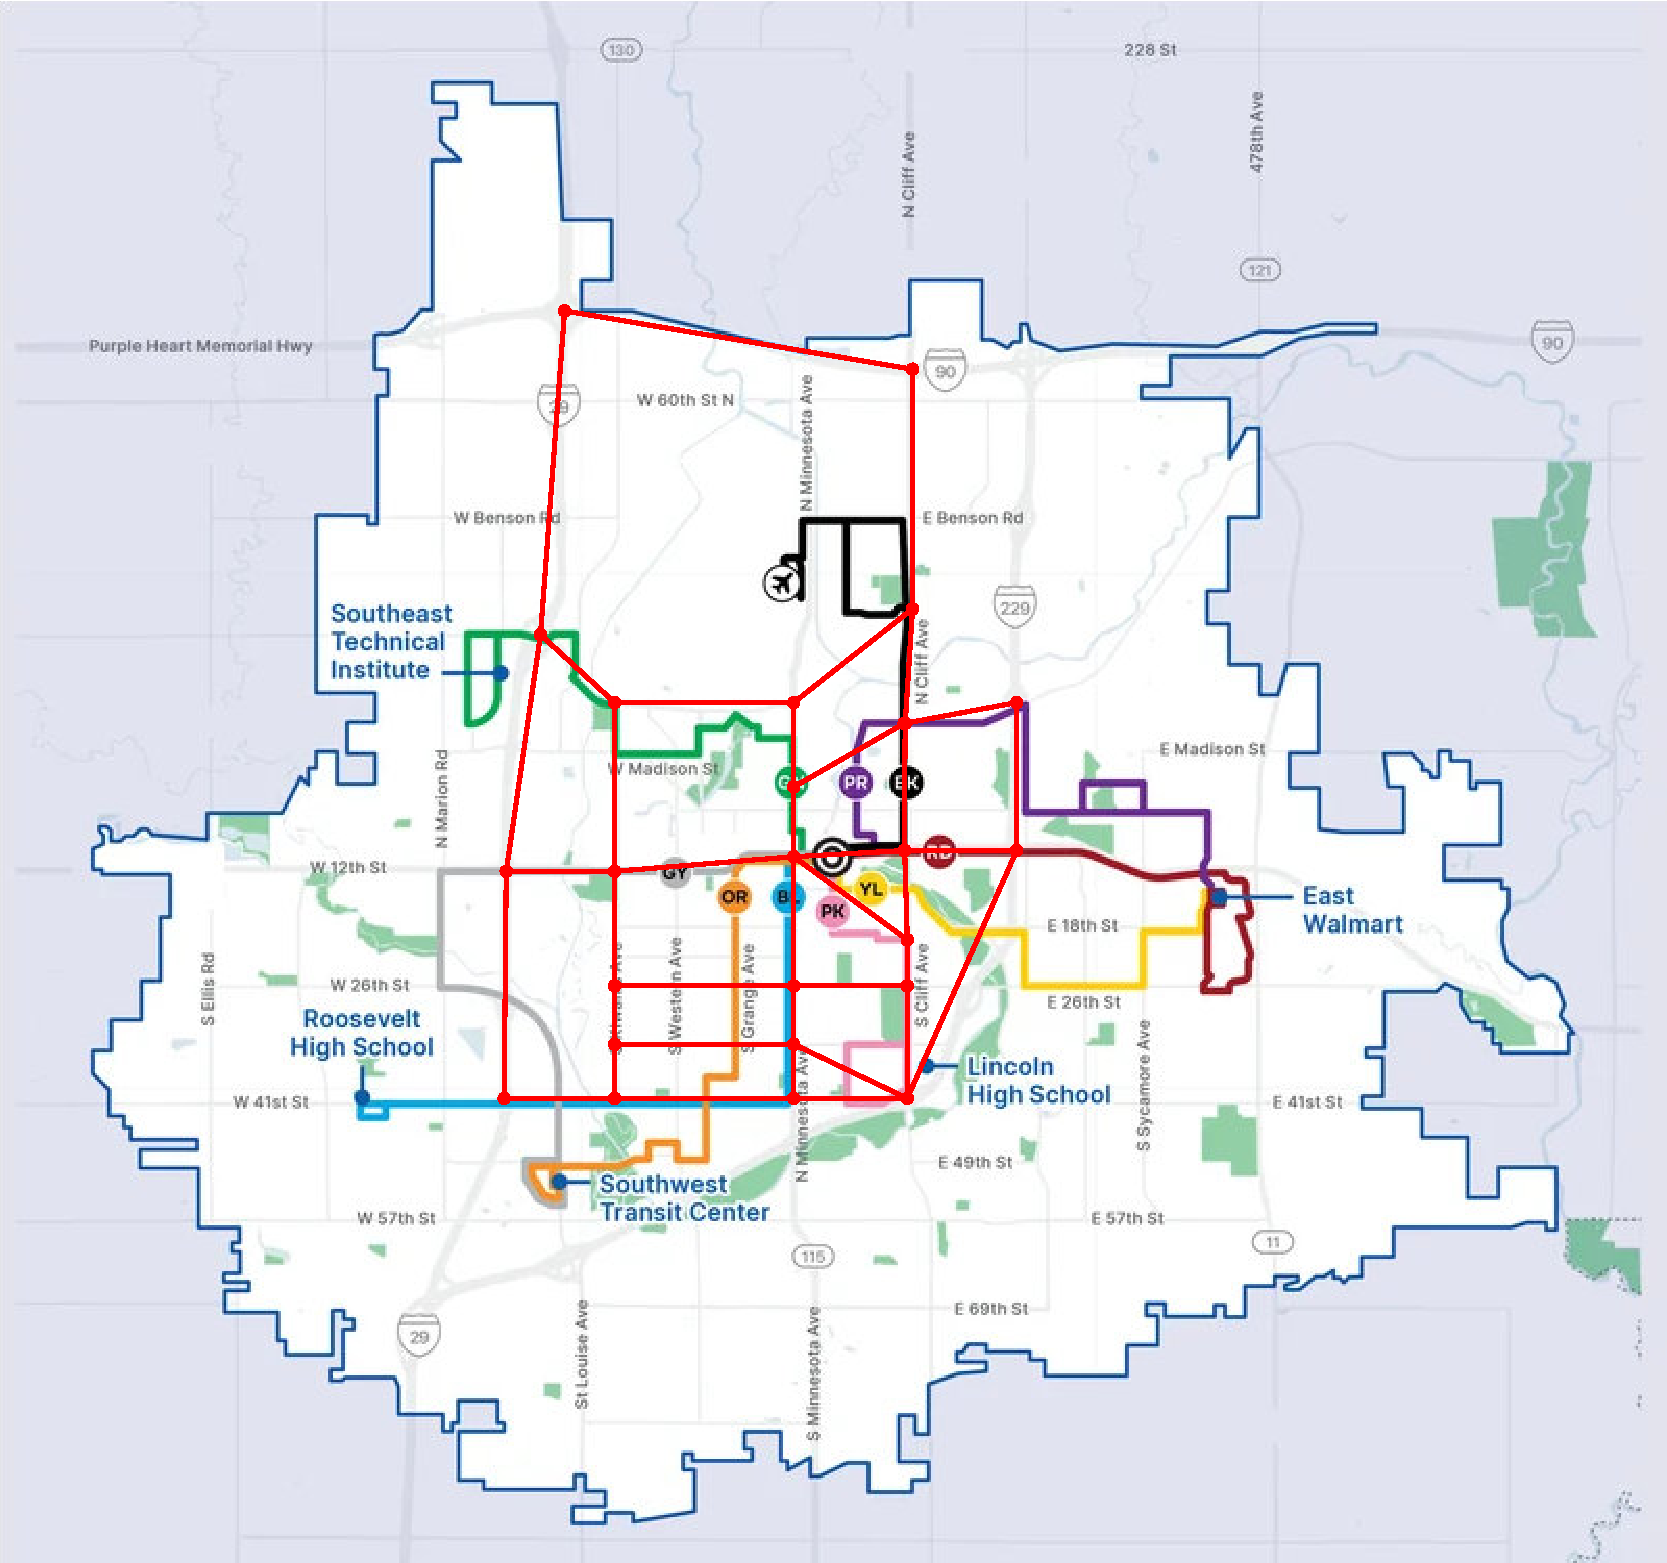
\includegraphics[width=.7\linewidth]{road_network_on_bus_map.pdf}
        \caption{Road network on bus map}
    \end{subfigure}%
    \begin{subfigure}{.45\textwidth}
        \centering
        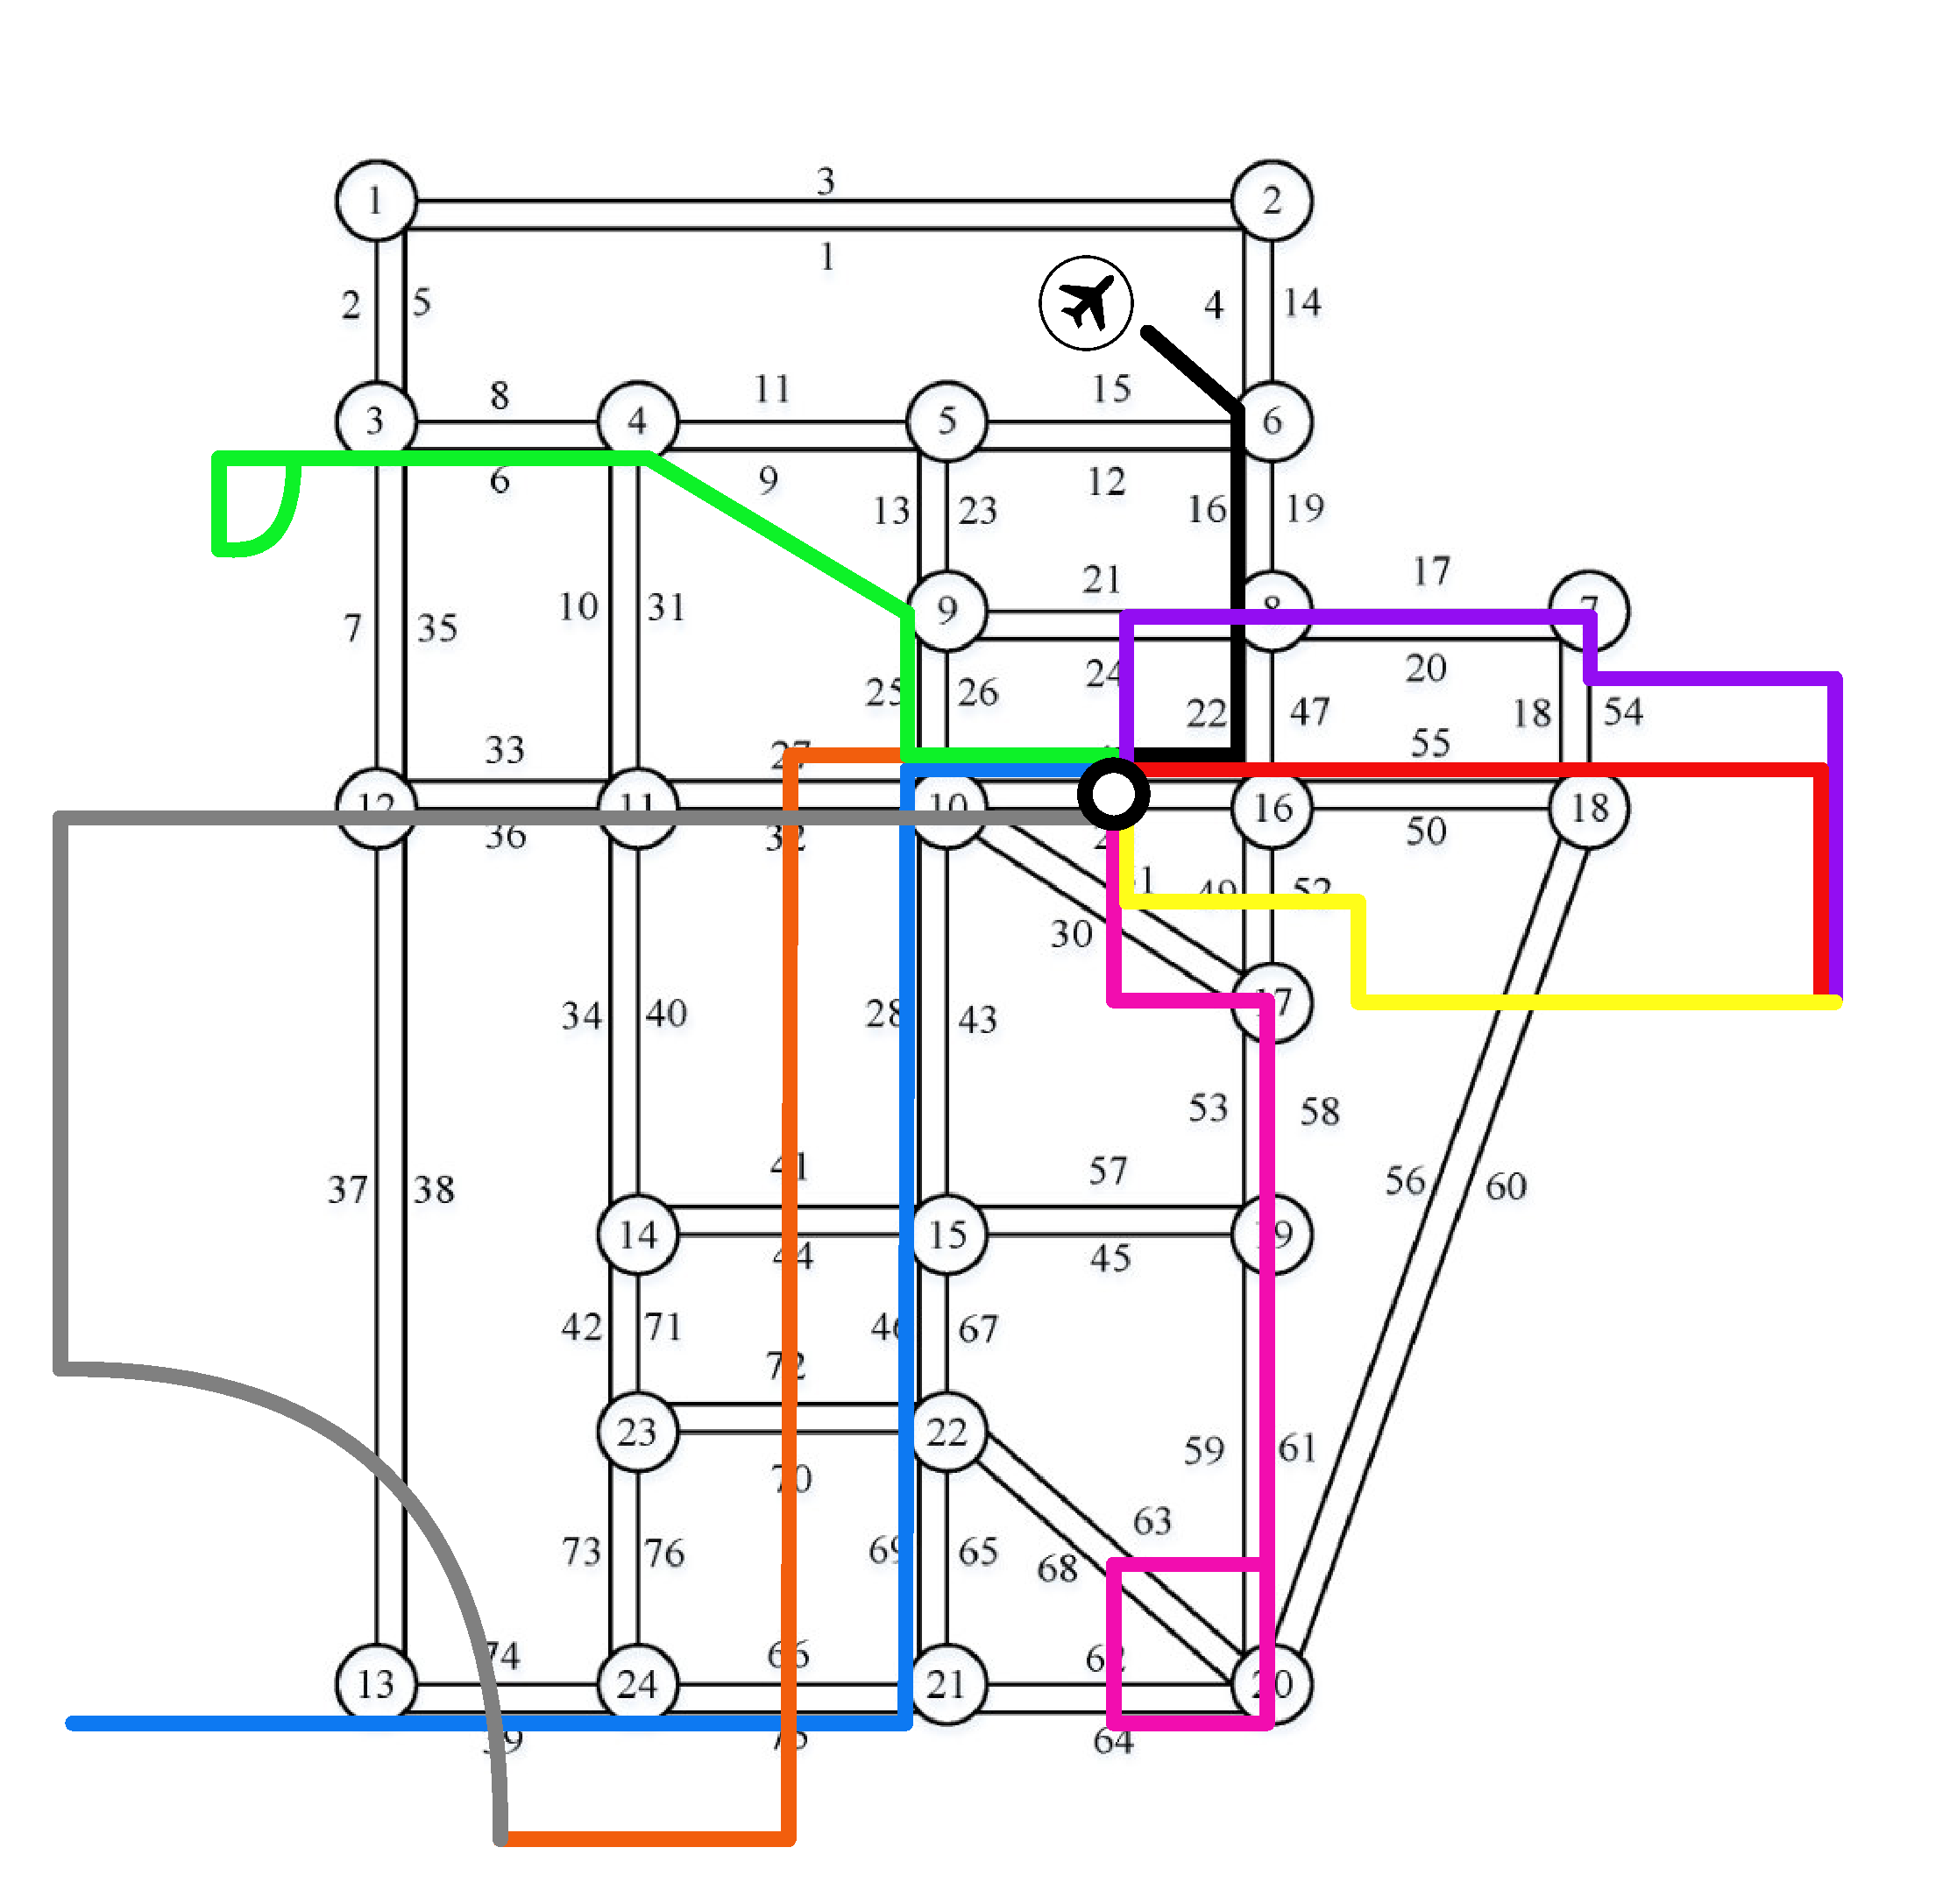
\includegraphics[width=.7\linewidth]{bus_network_on_road_map.pdf}
        \caption{Bus lines on road network}
    \end{subfigure}%
    \caption{Mapping between the bus lines and the simplified road network}
    \label{fig:mapping_bus}
\end{figure}

\begin{figure}
    \centering
    \begin{subfigure}{.45\textwidth}
        \centering
        \resizebox{.7\textwidth}{!}{%% Creator: Matplotlib, PGF backend
%%
%% To include the figure in your LaTeX document, write
%%   \input{<filename>.pgf}
%%
%% Make sure the required packages are loaded in your preamble
%%   \usepackage{pgf}
%%
%% Also ensure that all the required font packages are loaded; for instance,
%% the lmodern package is sometimes necessary when using math font.
%%   \usepackage{lmodern}
%%
%% Figures using additional raster images can only be included by \input if
%% they are in the same directory as the main LaTeX file. For loading figures
%% from other directories you can use the `import` package
%%   \usepackage{import}
%%
%% and then include the figures with
%%   \import{<path to file>}{<filename>.pgf}
%%
%% Matplotlib used the following preamble
%%   \def\mathdefault#1{#1}
%%   \everymath=\expandafter{\the\everymath\displaystyle}
%%   
%%   \ifdefined\pdftexversion\else  % non-pdftex case.
%%     \usepackage{fontspec}
%%     \setmainfont{DejaVuSerif.ttf}[Path=\detokenize{C:/Users/arsju/anaconda3/envs/Basic/Lib/site-packages/matplotlib/mpl-data/fonts/ttf/}]
%%     \setsansfont{DejaVuSans.ttf}[Path=\detokenize{C:/Users/arsju/anaconda3/envs/Basic/Lib/site-packages/matplotlib/mpl-data/fonts/ttf/}]
%%     \setmonofont{DejaVuSansMono.ttf}[Path=\detokenize{C:/Users/arsju/anaconda3/envs/Basic/Lib/site-packages/matplotlib/mpl-data/fonts/ttf/}]
%%   \fi
%%   \makeatletter\@ifpackageloaded{underscore}{}{\usepackage[strings]{underscore}}\makeatother
%%
\begingroup%
\makeatletter%
\begin{pgfpicture}%
\pgfpathrectangle{\pgfpointorigin}{\pgfqpoint{7.000000in}{7.000000in}}%
\pgfusepath{use as bounding box, clip}%
\begin{pgfscope}%
\pgfsetbuttcap%
\pgfsetmiterjoin%
\definecolor{currentfill}{rgb}{1.000000,1.000000,1.000000}%
\pgfsetfillcolor{currentfill}%
\pgfsetlinewidth{0.000000pt}%
\definecolor{currentstroke}{rgb}{1.000000,1.000000,1.000000}%
\pgfsetstrokecolor{currentstroke}%
\pgfsetdash{}{0pt}%
\pgfpathmoveto{\pgfqpoint{0.000000in}{0.000000in}}%
\pgfpathlineto{\pgfqpoint{7.000000in}{0.000000in}}%
\pgfpathlineto{\pgfqpoint{7.000000in}{7.000000in}}%
\pgfpathlineto{\pgfqpoint{0.000000in}{7.000000in}}%
\pgfpathlineto{\pgfqpoint{0.000000in}{0.000000in}}%
\pgfpathclose%
\pgfusepath{fill}%
\end{pgfscope}%
\begin{pgfscope}%
\pgfsetbuttcap%
\pgfsetmiterjoin%
\definecolor{currentfill}{rgb}{1.000000,1.000000,1.000000}%
\pgfsetfillcolor{currentfill}%
\pgfsetlinewidth{0.000000pt}%
\definecolor{currentstroke}{rgb}{0.000000,0.000000,0.000000}%
\pgfsetstrokecolor{currentstroke}%
\pgfsetstrokeopacity{0.000000}%
\pgfsetdash{}{0pt}%
\pgfpathmoveto{\pgfqpoint{1.419783in}{0.770000in}}%
\pgfpathlineto{\pgfqpoint{5.755217in}{0.770000in}}%
\pgfpathlineto{\pgfqpoint{5.755217in}{6.160000in}}%
\pgfpathlineto{\pgfqpoint{1.419783in}{6.160000in}}%
\pgfpathlineto{\pgfqpoint{1.419783in}{0.770000in}}%
\pgfpathclose%
\pgfusepath{fill}%
\end{pgfscope}%
\begin{pgfscope}%
\pgfpathrectangle{\pgfqpoint{1.419783in}{0.770000in}}{\pgfqpoint{4.335435in}{5.390000in}}%
\pgfusepath{clip}%
\pgfsetrectcap%
\pgfsetroundjoin%
\pgfsetlinewidth{0.940526pt}%
\definecolor{currentstroke}{rgb}{0.501961,0.501961,0.501961}%
\pgfsetstrokecolor{currentstroke}%
\pgfsetstrokeopacity{0.500000}%
\pgfsetdash{}{0pt}%
\pgfpathmoveto{\pgfqpoint{1.616848in}{5.915000in}}%
\pgfpathlineto{\pgfqpoint{4.492935in}{5.915000in}}%
\pgfusepath{stroke}%
\end{pgfscope}%
\begin{pgfscope}%
\pgfpathrectangle{\pgfqpoint{1.419783in}{0.770000in}}{\pgfqpoint{4.335435in}{5.390000in}}%
\pgfusepath{clip}%
\pgfsetrectcap%
\pgfsetroundjoin%
\pgfsetlinewidth{1.698278pt}%
\definecolor{currentstroke}{rgb}{0.501961,0.501961,0.501961}%
\pgfsetstrokecolor{currentstroke}%
\pgfsetstrokeopacity{0.500000}%
\pgfsetdash{}{0pt}%
\pgfpathmoveto{\pgfqpoint{1.616848in}{5.915000in}}%
\pgfpathlineto{\pgfqpoint{1.616848in}{5.169348in}}%
\pgfusepath{stroke}%
\end{pgfscope}%
\begin{pgfscope}%
\pgfpathrectangle{\pgfqpoint{1.419783in}{0.770000in}}{\pgfqpoint{4.335435in}{5.390000in}}%
\pgfusepath{clip}%
\pgfsetrectcap%
\pgfsetroundjoin%
\pgfsetlinewidth{0.945680pt}%
\definecolor{currentstroke}{rgb}{0.501961,0.501961,0.501961}%
\pgfsetstrokecolor{currentstroke}%
\pgfsetstrokeopacity{0.500000}%
\pgfsetdash{}{0pt}%
\pgfpathmoveto{\pgfqpoint{4.492935in}{5.915000in}}%
\pgfpathlineto{\pgfqpoint{1.616848in}{5.915000in}}%
\pgfusepath{stroke}%
\end{pgfscope}%
\begin{pgfscope}%
\pgfpathrectangle{\pgfqpoint{1.419783in}{0.770000in}}{\pgfqpoint{4.335435in}{5.390000in}}%
\pgfusepath{clip}%
\pgfsetrectcap%
\pgfsetroundjoin%
\pgfsetlinewidth{1.248080pt}%
\definecolor{currentstroke}{rgb}{0.501961,0.501961,0.501961}%
\pgfsetstrokecolor{currentstroke}%
\pgfsetstrokeopacity{0.500000}%
\pgfsetdash{}{0pt}%
\pgfpathmoveto{\pgfqpoint{4.492935in}{5.915000in}}%
\pgfpathlineto{\pgfqpoint{4.492935in}{5.169348in}}%
\pgfusepath{stroke}%
\end{pgfscope}%
\begin{pgfscope}%
\pgfpathrectangle{\pgfqpoint{1.419783in}{0.770000in}}{\pgfqpoint{4.335435in}{5.390000in}}%
\pgfusepath{clip}%
\pgfsetrectcap%
\pgfsetroundjoin%
\pgfsetlinewidth{1.693124pt}%
\definecolor{currentstroke}{rgb}{0.501961,0.501961,0.501961}%
\pgfsetstrokecolor{currentstroke}%
\pgfsetstrokeopacity{0.500000}%
\pgfsetdash{}{0pt}%
\pgfpathmoveto{\pgfqpoint{1.616848in}{5.169348in}}%
\pgfpathlineto{\pgfqpoint{1.616848in}{5.915000in}}%
\pgfusepath{stroke}%
\end{pgfscope}%
\begin{pgfscope}%
\pgfpathrectangle{\pgfqpoint{1.419783in}{0.770000in}}{\pgfqpoint{4.335435in}{5.390000in}}%
\pgfusepath{clip}%
\pgfsetrectcap%
\pgfsetroundjoin%
\pgfsetlinewidth{2.931204pt}%
\definecolor{currentstroke}{rgb}{0.501961,0.501961,0.501961}%
\pgfsetstrokecolor{currentstroke}%
\pgfsetstrokeopacity{0.500000}%
\pgfsetdash{}{0pt}%
\pgfpathmoveto{\pgfqpoint{1.616848in}{5.169348in}}%
\pgfpathlineto{\pgfqpoint{2.469022in}{5.169348in}}%
\pgfusepath{stroke}%
\end{pgfscope}%
\begin{pgfscope}%
\pgfpathrectangle{\pgfqpoint{1.419783in}{0.770000in}}{\pgfqpoint{4.335435in}{5.390000in}}%
\pgfusepath{clip}%
\pgfsetrectcap%
\pgfsetroundjoin%
\pgfsetlinewidth{2.098514pt}%
\definecolor{currentstroke}{rgb}{0.501961,0.501961,0.501961}%
\pgfsetstrokecolor{currentstroke}%
\pgfsetstrokeopacity{0.500000}%
\pgfsetdash{}{0pt}%
\pgfpathmoveto{\pgfqpoint{1.616848in}{5.169348in}}%
\pgfpathlineto{\pgfqpoint{1.616848in}{3.891087in}}%
\pgfusepath{stroke}%
\end{pgfscope}%
\begin{pgfscope}%
\pgfpathrectangle{\pgfqpoint{1.419783in}{0.770000in}}{\pgfqpoint{4.335435in}{5.390000in}}%
\pgfusepath{clip}%
\pgfsetrectcap%
\pgfsetroundjoin%
\pgfsetlinewidth{2.936353pt}%
\definecolor{currentstroke}{rgb}{0.501961,0.501961,0.501961}%
\pgfsetstrokecolor{currentstroke}%
\pgfsetstrokeopacity{0.500000}%
\pgfsetdash{}{0pt}%
\pgfpathmoveto{\pgfqpoint{2.469022in}{5.169348in}}%
\pgfpathlineto{\pgfqpoint{1.616848in}{5.169348in}}%
\pgfusepath{stroke}%
\end{pgfscope}%
\begin{pgfscope}%
\pgfpathrectangle{\pgfqpoint{1.419783in}{0.770000in}}{\pgfqpoint{4.335435in}{5.390000in}}%
\pgfusepath{clip}%
\pgfsetrectcap%
\pgfsetroundjoin%
\pgfsetlinewidth{3.766880pt}%
\definecolor{currentstroke}{rgb}{0.501961,0.501961,0.501961}%
\pgfsetstrokecolor{currentstroke}%
\pgfsetstrokeopacity{0.500000}%
\pgfsetdash{}{0pt}%
\pgfpathmoveto{\pgfqpoint{2.469022in}{5.169348in}}%
\pgfpathlineto{\pgfqpoint{3.427717in}{5.169348in}}%
\pgfusepath{stroke}%
\end{pgfscope}%
\begin{pgfscope}%
\pgfpathrectangle{\pgfqpoint{1.419783in}{0.770000in}}{\pgfqpoint{4.335435in}{5.390000in}}%
\pgfusepath{clip}%
\pgfsetrectcap%
\pgfsetroundjoin%
\pgfsetlinewidth{1.089388pt}%
\definecolor{currentstroke}{rgb}{0.501961,0.501961,0.501961}%
\pgfsetstrokecolor{currentstroke}%
\pgfsetstrokeopacity{0.500000}%
\pgfsetdash{}{0pt}%
\pgfpathmoveto{\pgfqpoint{2.469022in}{5.169348in}}%
\pgfpathlineto{\pgfqpoint{2.469022in}{3.891087in}}%
\pgfusepath{stroke}%
\end{pgfscope}%
\begin{pgfscope}%
\pgfpathrectangle{\pgfqpoint{1.419783in}{0.770000in}}{\pgfqpoint{4.335435in}{5.390000in}}%
\pgfusepath{clip}%
\pgfsetrectcap%
\pgfsetroundjoin%
\pgfsetlinewidth{3.772464pt}%
\definecolor{currentstroke}{rgb}{0.501961,0.501961,0.501961}%
\pgfsetstrokecolor{currentstroke}%
\pgfsetstrokeopacity{0.500000}%
\pgfsetdash{}{0pt}%
\pgfpathmoveto{\pgfqpoint{3.427717in}{5.169348in}}%
\pgfpathlineto{\pgfqpoint{2.469022in}{5.169348in}}%
\pgfusepath{stroke}%
\end{pgfscope}%
\begin{pgfscope}%
\pgfpathrectangle{\pgfqpoint{1.419783in}{0.770000in}}{\pgfqpoint{4.335435in}{5.390000in}}%
\pgfusepath{clip}%
\pgfsetrectcap%
\pgfsetroundjoin%
\pgfsetlinewidth{1.839225pt}%
\definecolor{currentstroke}{rgb}{0.501961,0.501961,0.501961}%
\pgfsetstrokecolor{currentstroke}%
\pgfsetstrokeopacity{0.500000}%
\pgfsetdash{}{0pt}%
\pgfpathmoveto{\pgfqpoint{3.427717in}{5.169348in}}%
\pgfpathlineto{\pgfqpoint{4.492935in}{5.169348in}}%
\pgfusepath{stroke}%
\end{pgfscope}%
\begin{pgfscope}%
\pgfpathrectangle{\pgfqpoint{1.419783in}{0.770000in}}{\pgfqpoint{4.335435in}{5.390000in}}%
\pgfusepath{clip}%
\pgfsetrectcap%
\pgfsetroundjoin%
\pgfsetlinewidth{3.300646pt}%
\definecolor{currentstroke}{rgb}{0.501961,0.501961,0.501961}%
\pgfsetstrokecolor{currentstroke}%
\pgfsetstrokeopacity{0.500000}%
\pgfsetdash{}{0pt}%
\pgfpathmoveto{\pgfqpoint{3.427717in}{5.169348in}}%
\pgfpathlineto{\pgfqpoint{3.427717in}{4.530217in}}%
\pgfusepath{stroke}%
\end{pgfscope}%
\begin{pgfscope}%
\pgfpathrectangle{\pgfqpoint{1.419783in}{0.770000in}}{\pgfqpoint{4.335435in}{5.390000in}}%
\pgfusepath{clip}%
\pgfsetrectcap%
\pgfsetroundjoin%
\pgfsetlinewidth{1.253234pt}%
\definecolor{currentstroke}{rgb}{0.501961,0.501961,0.501961}%
\pgfsetstrokecolor{currentstroke}%
\pgfsetstrokeopacity{0.500000}%
\pgfsetdash{}{0pt}%
\pgfpathmoveto{\pgfqpoint{4.492935in}{5.169348in}}%
\pgfpathlineto{\pgfqpoint{4.492935in}{5.915000in}}%
\pgfusepath{stroke}%
\end{pgfscope}%
\begin{pgfscope}%
\pgfpathrectangle{\pgfqpoint{1.419783in}{0.770000in}}{\pgfqpoint{4.335435in}{5.390000in}}%
\pgfusepath{clip}%
\pgfsetrectcap%
\pgfsetroundjoin%
\pgfsetlinewidth{1.840990pt}%
\definecolor{currentstroke}{rgb}{0.501961,0.501961,0.501961}%
\pgfsetstrokecolor{currentstroke}%
\pgfsetstrokeopacity{0.500000}%
\pgfsetdash{}{0pt}%
\pgfpathmoveto{\pgfqpoint{4.492935in}{5.169348in}}%
\pgfpathlineto{\pgfqpoint{3.427717in}{5.169348in}}%
\pgfusepath{stroke}%
\end{pgfscope}%
\begin{pgfscope}%
\pgfpathrectangle{\pgfqpoint{1.419783in}{0.770000in}}{\pgfqpoint{4.335435in}{5.390000in}}%
\pgfusepath{clip}%
\pgfsetrectcap%
\pgfsetroundjoin%
\pgfsetlinewidth{2.612310pt}%
\definecolor{currentstroke}{rgb}{0.501961,0.501961,0.501961}%
\pgfsetstrokecolor{currentstroke}%
\pgfsetstrokeopacity{0.500000}%
\pgfsetdash{}{0pt}%
\pgfpathmoveto{\pgfqpoint{4.492935in}{5.169348in}}%
\pgfpathlineto{\pgfqpoint{4.492935in}{4.530217in}}%
\pgfusepath{stroke}%
\end{pgfscope}%
\begin{pgfscope}%
\pgfpathrectangle{\pgfqpoint{1.419783in}{0.770000in}}{\pgfqpoint{4.335435in}{5.390000in}}%
\pgfusepath{clip}%
\pgfsetrectcap%
\pgfsetroundjoin%
\pgfsetlinewidth{2.530626pt}%
\definecolor{currentstroke}{rgb}{0.501961,0.501961,0.501961}%
\pgfsetstrokecolor{currentstroke}%
\pgfsetstrokeopacity{0.500000}%
\pgfsetdash{}{0pt}%
\pgfpathmoveto{\pgfqpoint{5.558152in}{4.530217in}}%
\pgfpathlineto{\pgfqpoint{4.492935in}{4.530217in}}%
\pgfusepath{stroke}%
\end{pgfscope}%
\begin{pgfscope}%
\pgfpathrectangle{\pgfqpoint{1.419783in}{0.770000in}}{\pgfqpoint{4.335435in}{5.390000in}}%
\pgfusepath{clip}%
\pgfsetrectcap%
\pgfsetroundjoin%
\pgfsetlinewidth{3.304215pt}%
\definecolor{currentstroke}{rgb}{0.501961,0.501961,0.501961}%
\pgfsetstrokecolor{currentstroke}%
\pgfsetstrokeopacity{0.500000}%
\pgfsetdash{}{0pt}%
\pgfpathmoveto{\pgfqpoint{5.558152in}{4.530217in}}%
\pgfpathlineto{\pgfqpoint{5.558152in}{3.891087in}}%
\pgfusepath{stroke}%
\end{pgfscope}%
\begin{pgfscope}%
\pgfpathrectangle{\pgfqpoint{1.419783in}{0.770000in}}{\pgfqpoint{4.335435in}{5.390000in}}%
\pgfusepath{clip}%
\pgfsetrectcap%
\pgfsetroundjoin%
\pgfsetlinewidth{2.619230pt}%
\definecolor{currentstroke}{rgb}{0.501961,0.501961,0.501961}%
\pgfsetstrokecolor{currentstroke}%
\pgfsetstrokeopacity{0.500000}%
\pgfsetdash{}{0pt}%
\pgfpathmoveto{\pgfqpoint{4.492935in}{4.530217in}}%
\pgfpathlineto{\pgfqpoint{4.492935in}{5.169348in}}%
\pgfusepath{stroke}%
\end{pgfscope}%
\begin{pgfscope}%
\pgfpathrectangle{\pgfqpoint{1.419783in}{0.770000in}}{\pgfqpoint{4.335435in}{5.390000in}}%
\pgfusepath{clip}%
\pgfsetrectcap%
\pgfsetroundjoin%
\pgfsetlinewidth{2.517976pt}%
\definecolor{currentstroke}{rgb}{0.501961,0.501961,0.501961}%
\pgfsetstrokecolor{currentstroke}%
\pgfsetstrokeopacity{0.500000}%
\pgfsetdash{}{0pt}%
\pgfpathmoveto{\pgfqpoint{4.492935in}{4.530217in}}%
\pgfpathlineto{\pgfqpoint{5.558152in}{4.530217in}}%
\pgfusepath{stroke}%
\end{pgfscope}%
\begin{pgfscope}%
\pgfpathrectangle{\pgfqpoint{1.419783in}{0.770000in}}{\pgfqpoint{4.335435in}{5.390000in}}%
\pgfusepath{clip}%
\pgfsetrectcap%
\pgfsetroundjoin%
\pgfsetlinewidth{1.438957pt}%
\definecolor{currentstroke}{rgb}{0.501961,0.501961,0.501961}%
\pgfsetstrokecolor{currentstroke}%
\pgfsetstrokeopacity{0.500000}%
\pgfsetdash{}{0pt}%
\pgfpathmoveto{\pgfqpoint{4.492935in}{4.530217in}}%
\pgfpathlineto{\pgfqpoint{3.427717in}{4.530217in}}%
\pgfusepath{stroke}%
\end{pgfscope}%
\begin{pgfscope}%
\pgfpathrectangle{\pgfqpoint{1.419783in}{0.770000in}}{\pgfqpoint{4.335435in}{5.390000in}}%
\pgfusepath{clip}%
\pgfsetrectcap%
\pgfsetroundjoin%
\pgfsetlinewidth{1.753615pt}%
\definecolor{currentstroke}{rgb}{0.501961,0.501961,0.501961}%
\pgfsetstrokecolor{currentstroke}%
\pgfsetstrokeopacity{0.500000}%
\pgfsetdash{}{0pt}%
\pgfpathmoveto{\pgfqpoint{4.492935in}{4.530217in}}%
\pgfpathlineto{\pgfqpoint{4.492935in}{3.891087in}}%
\pgfusepath{stroke}%
\end{pgfscope}%
\begin{pgfscope}%
\pgfpathrectangle{\pgfqpoint{1.419783in}{0.770000in}}{\pgfqpoint{4.335435in}{5.390000in}}%
\pgfusepath{clip}%
\pgfsetrectcap%
\pgfsetroundjoin%
\pgfsetlinewidth{3.304464pt}%
\definecolor{currentstroke}{rgb}{0.501961,0.501961,0.501961}%
\pgfsetstrokecolor{currentstroke}%
\pgfsetstrokeopacity{0.500000}%
\pgfsetdash{}{0pt}%
\pgfpathmoveto{\pgfqpoint{3.427717in}{4.530217in}}%
\pgfpathlineto{\pgfqpoint{3.427717in}{5.169348in}}%
\pgfusepath{stroke}%
\end{pgfscope}%
\begin{pgfscope}%
\pgfpathrectangle{\pgfqpoint{1.419783in}{0.770000in}}{\pgfqpoint{4.335435in}{5.390000in}}%
\pgfusepath{clip}%
\pgfsetrectcap%
\pgfsetroundjoin%
\pgfsetlinewidth{1.429240pt}%
\definecolor{currentstroke}{rgb}{0.501961,0.501961,0.501961}%
\pgfsetstrokecolor{currentstroke}%
\pgfsetstrokeopacity{0.500000}%
\pgfsetdash{}{0pt}%
\pgfpathmoveto{\pgfqpoint{3.427717in}{4.530217in}}%
\pgfpathlineto{\pgfqpoint{4.492935in}{4.530217in}}%
\pgfusepath{stroke}%
\end{pgfscope}%
\begin{pgfscope}%
\pgfpathrectangle{\pgfqpoint{1.419783in}{0.770000in}}{\pgfqpoint{4.335435in}{5.390000in}}%
\pgfusepath{clip}%
\pgfsetrectcap%
\pgfsetroundjoin%
\pgfsetlinewidth{4.547759pt}%
\definecolor{currentstroke}{rgb}{0.501961,0.501961,0.501961}%
\pgfsetstrokecolor{currentstroke}%
\pgfsetstrokeopacity{0.500000}%
\pgfsetdash{}{0pt}%
\pgfpathmoveto{\pgfqpoint{3.427717in}{4.530217in}}%
\pgfpathlineto{\pgfqpoint{3.427717in}{3.891087in}}%
\pgfusepath{stroke}%
\end{pgfscope}%
\begin{pgfscope}%
\pgfpathrectangle{\pgfqpoint{1.419783in}{0.770000in}}{\pgfqpoint{4.335435in}{5.390000in}}%
\pgfusepath{clip}%
\pgfsetrectcap%
\pgfsetroundjoin%
\pgfsetlinewidth{4.562771pt}%
\definecolor{currentstroke}{rgb}{0.501961,0.501961,0.501961}%
\pgfsetstrokecolor{currentstroke}%
\pgfsetstrokeopacity{0.500000}%
\pgfsetdash{}{0pt}%
\pgfpathmoveto{\pgfqpoint{3.427717in}{3.891087in}}%
\pgfpathlineto{\pgfqpoint{3.427717in}{4.530217in}}%
\pgfusepath{stroke}%
\end{pgfscope}%
\begin{pgfscope}%
\pgfpathrectangle{\pgfqpoint{1.419783in}{0.770000in}}{\pgfqpoint{4.335435in}{5.390000in}}%
\pgfusepath{clip}%
\pgfsetrectcap%
\pgfsetroundjoin%
\pgfsetlinewidth{3.707399pt}%
\definecolor{currentstroke}{rgb}{0.501961,0.501961,0.501961}%
\pgfsetstrokecolor{currentstroke}%
\pgfsetstrokeopacity{0.500000}%
\pgfsetdash{}{0pt}%
\pgfpathmoveto{\pgfqpoint{3.427717in}{3.891087in}}%
\pgfpathlineto{\pgfqpoint{2.469022in}{3.891087in}}%
\pgfusepath{stroke}%
\end{pgfscope}%
\begin{pgfscope}%
\pgfpathrectangle{\pgfqpoint{1.419783in}{0.770000in}}{\pgfqpoint{4.335435in}{5.390000in}}%
\pgfusepath{clip}%
\pgfsetrectcap%
\pgfsetroundjoin%
\pgfsetlinewidth{4.836738pt}%
\definecolor{currentstroke}{rgb}{0.501961,0.501961,0.501961}%
\pgfsetstrokecolor{currentstroke}%
\pgfsetstrokeopacity{0.500000}%
\pgfsetdash{}{0pt}%
\pgfpathmoveto{\pgfqpoint{3.427717in}{3.891087in}}%
\pgfpathlineto{\pgfqpoint{3.427717in}{2.506304in}}%
\pgfusepath{stroke}%
\end{pgfscope}%
\begin{pgfscope}%
\pgfpathrectangle{\pgfqpoint{1.419783in}{0.770000in}}{\pgfqpoint{4.335435in}{5.390000in}}%
\pgfusepath{clip}%
\pgfsetrectcap%
\pgfsetroundjoin%
\pgfsetlinewidth{2.310273pt}%
\definecolor{currentstroke}{rgb}{0.501961,0.501961,0.501961}%
\pgfsetstrokecolor{currentstroke}%
\pgfsetstrokeopacity{0.500000}%
\pgfsetdash{}{0pt}%
\pgfpathmoveto{\pgfqpoint{3.427717in}{3.891087in}}%
\pgfpathlineto{\pgfqpoint{4.492935in}{3.891087in}}%
\pgfusepath{stroke}%
\end{pgfscope}%
\begin{pgfscope}%
\pgfpathrectangle{\pgfqpoint{1.419783in}{0.770000in}}{\pgfqpoint{4.335435in}{5.390000in}}%
\pgfusepath{clip}%
\pgfsetrectcap%
\pgfsetroundjoin%
\pgfsetlinewidth{1.693849pt}%
\definecolor{currentstroke}{rgb}{0.501961,0.501961,0.501961}%
\pgfsetstrokecolor{currentstroke}%
\pgfsetstrokeopacity{0.500000}%
\pgfsetdash{}{0pt}%
\pgfpathmoveto{\pgfqpoint{3.427717in}{3.891087in}}%
\pgfpathlineto{\pgfqpoint{4.492935in}{3.251957in}}%
\pgfusepath{stroke}%
\end{pgfscope}%
\begin{pgfscope}%
\pgfpathrectangle{\pgfqpoint{1.419783in}{0.770000in}}{\pgfqpoint{4.335435in}{5.390000in}}%
\pgfusepath{clip}%
\pgfsetrectcap%
\pgfsetroundjoin%
\pgfsetlinewidth{1.109864pt}%
\definecolor{currentstroke}{rgb}{0.501961,0.501961,0.501961}%
\pgfsetstrokecolor{currentstroke}%
\pgfsetstrokeopacity{0.500000}%
\pgfsetdash{}{0pt}%
\pgfpathmoveto{\pgfqpoint{2.469022in}{3.891087in}}%
\pgfpathlineto{\pgfqpoint{2.469022in}{5.169348in}}%
\pgfusepath{stroke}%
\end{pgfscope}%
\begin{pgfscope}%
\pgfpathrectangle{\pgfqpoint{1.419783in}{0.770000in}}{\pgfqpoint{4.335435in}{5.390000in}}%
\pgfusepath{clip}%
\pgfsetrectcap%
\pgfsetroundjoin%
\pgfsetlinewidth{3.682312pt}%
\definecolor{currentstroke}{rgb}{0.501961,0.501961,0.501961}%
\pgfsetstrokecolor{currentstroke}%
\pgfsetstrokeopacity{0.500000}%
\pgfsetdash{}{0pt}%
\pgfpathmoveto{\pgfqpoint{2.469022in}{3.891087in}}%
\pgfpathlineto{\pgfqpoint{3.427717in}{3.891087in}}%
\pgfusepath{stroke}%
\end{pgfscope}%
\begin{pgfscope}%
\pgfpathrectangle{\pgfqpoint{1.419783in}{0.770000in}}{\pgfqpoint{4.335435in}{5.390000in}}%
\pgfusepath{clip}%
\pgfsetrectcap%
\pgfsetroundjoin%
\pgfsetlinewidth{1.749480pt}%
\definecolor{currentstroke}{rgb}{0.501961,0.501961,0.501961}%
\pgfsetstrokecolor{currentstroke}%
\pgfsetstrokeopacity{0.500000}%
\pgfsetdash{}{0pt}%
\pgfpathmoveto{\pgfqpoint{2.469022in}{3.891087in}}%
\pgfpathlineto{\pgfqpoint{1.616848in}{3.891087in}}%
\pgfusepath{stroke}%
\end{pgfscope}%
\begin{pgfscope}%
\pgfpathrectangle{\pgfqpoint{1.419783in}{0.770000in}}{\pgfqpoint{4.335435in}{5.390000in}}%
\pgfusepath{clip}%
\pgfsetrectcap%
\pgfsetroundjoin%
\pgfsetlinewidth{2.044741pt}%
\definecolor{currentstroke}{rgb}{0.501961,0.501961,0.501961}%
\pgfsetstrokecolor{currentstroke}%
\pgfsetstrokeopacity{0.500000}%
\pgfsetdash{}{0pt}%
\pgfpathmoveto{\pgfqpoint{2.469022in}{3.891087in}}%
\pgfpathlineto{\pgfqpoint{2.469022in}{2.506304in}}%
\pgfusepath{stroke}%
\end{pgfscope}%
\begin{pgfscope}%
\pgfpathrectangle{\pgfqpoint{1.419783in}{0.770000in}}{\pgfqpoint{4.335435in}{5.390000in}}%
\pgfusepath{clip}%
\pgfsetrectcap%
\pgfsetroundjoin%
\pgfsetlinewidth{2.088211pt}%
\definecolor{currentstroke}{rgb}{0.501961,0.501961,0.501961}%
\pgfsetstrokecolor{currentstroke}%
\pgfsetstrokeopacity{0.500000}%
\pgfsetdash{}{0pt}%
\pgfpathmoveto{\pgfqpoint{1.616848in}{3.891087in}}%
\pgfpathlineto{\pgfqpoint{1.616848in}{5.169348in}}%
\pgfusepath{stroke}%
\end{pgfscope}%
\begin{pgfscope}%
\pgfpathrectangle{\pgfqpoint{1.419783in}{0.770000in}}{\pgfqpoint{4.335435in}{5.390000in}}%
\pgfusepath{clip}%
\pgfsetrectcap%
\pgfsetroundjoin%
\pgfsetlinewidth{1.757866pt}%
\definecolor{currentstroke}{rgb}{0.501961,0.501961,0.501961}%
\pgfsetstrokecolor{currentstroke}%
\pgfsetstrokeopacity{0.500000}%
\pgfsetdash{}{0pt}%
\pgfpathmoveto{\pgfqpoint{1.616848in}{3.891087in}}%
\pgfpathlineto{\pgfqpoint{2.469022in}{3.891087in}}%
\pgfusepath{stroke}%
\end{pgfscope}%
\begin{pgfscope}%
\pgfpathrectangle{\pgfqpoint{1.419783in}{0.770000in}}{\pgfqpoint{4.335435in}{5.390000in}}%
\pgfusepath{clip}%
\pgfsetrectcap%
\pgfsetroundjoin%
\pgfsetlinewidth{2.573139pt}%
\definecolor{currentstroke}{rgb}{0.501961,0.501961,0.501961}%
\pgfsetstrokecolor{currentstroke}%
\pgfsetstrokeopacity{0.500000}%
\pgfsetdash{}{0pt}%
\pgfpathmoveto{\pgfqpoint{1.616848in}{3.891087in}}%
\pgfpathlineto{\pgfqpoint{1.616848in}{1.015000in}}%
\pgfusepath{stroke}%
\end{pgfscope}%
\begin{pgfscope}%
\pgfpathrectangle{\pgfqpoint{1.419783in}{0.770000in}}{\pgfqpoint{4.335435in}{5.390000in}}%
\pgfusepath{clip}%
\pgfsetrectcap%
\pgfsetroundjoin%
\pgfsetlinewidth{2.592134pt}%
\definecolor{currentstroke}{rgb}{0.501961,0.501961,0.501961}%
\pgfsetstrokecolor{currentstroke}%
\pgfsetstrokeopacity{0.500000}%
\pgfsetdash{}{0pt}%
\pgfpathmoveto{\pgfqpoint{1.616848in}{1.015000in}}%
\pgfpathlineto{\pgfqpoint{1.616848in}{3.891087in}}%
\pgfusepath{stroke}%
\end{pgfscope}%
\begin{pgfscope}%
\pgfpathrectangle{\pgfqpoint{1.419783in}{0.770000in}}{\pgfqpoint{4.335435in}{5.390000in}}%
\pgfusepath{clip}%
\pgfsetrectcap%
\pgfsetroundjoin%
\pgfsetlinewidth{2.325285pt}%
\definecolor{currentstroke}{rgb}{0.501961,0.501961,0.501961}%
\pgfsetstrokecolor{currentstroke}%
\pgfsetstrokeopacity{0.500000}%
\pgfsetdash{}{0pt}%
\pgfpathmoveto{\pgfqpoint{1.616848in}{1.015000in}}%
\pgfpathlineto{\pgfqpoint{2.469022in}{1.015000in}}%
\pgfusepath{stroke}%
\end{pgfscope}%
\begin{pgfscope}%
\pgfpathrectangle{\pgfqpoint{1.419783in}{0.770000in}}{\pgfqpoint{4.335435in}{5.390000in}}%
\pgfusepath{clip}%
\pgfsetrectcap%
\pgfsetroundjoin%
\pgfsetlinewidth{2.052656pt}%
\definecolor{currentstroke}{rgb}{0.501961,0.501961,0.501961}%
\pgfsetstrokecolor{currentstroke}%
\pgfsetstrokeopacity{0.500000}%
\pgfsetdash{}{0pt}%
\pgfpathmoveto{\pgfqpoint{2.469022in}{2.506304in}}%
\pgfpathlineto{\pgfqpoint{2.469022in}{3.891087in}}%
\pgfusepath{stroke}%
\end{pgfscope}%
\begin{pgfscope}%
\pgfpathrectangle{\pgfqpoint{1.419783in}{0.770000in}}{\pgfqpoint{4.335435in}{5.390000in}}%
\pgfusepath{clip}%
\pgfsetrectcap%
\pgfsetroundjoin%
\pgfsetlinewidth{1.888859pt}%
\definecolor{currentstroke}{rgb}{0.501961,0.501961,0.501961}%
\pgfsetstrokecolor{currentstroke}%
\pgfsetstrokeopacity{0.500000}%
\pgfsetdash{}{0pt}%
\pgfpathmoveto{\pgfqpoint{2.469022in}{2.506304in}}%
\pgfpathlineto{\pgfqpoint{3.427717in}{2.506304in}}%
\pgfusepath{stroke}%
\end{pgfscope}%
\begin{pgfscope}%
\pgfpathrectangle{\pgfqpoint{1.419783in}{0.770000in}}{\pgfqpoint{4.335435in}{5.390000in}}%
\pgfusepath{clip}%
\pgfsetrectcap%
\pgfsetroundjoin%
\pgfsetlinewidth{1.756117pt}%
\definecolor{currentstroke}{rgb}{0.501961,0.501961,0.501961}%
\pgfsetstrokecolor{currentstroke}%
\pgfsetstrokeopacity{0.500000}%
\pgfsetdash{}{0pt}%
\pgfpathmoveto{\pgfqpoint{2.469022in}{2.506304in}}%
\pgfpathlineto{\pgfqpoint{2.469022in}{1.867174in}}%
\pgfusepath{stroke}%
\end{pgfscope}%
\begin{pgfscope}%
\pgfpathrectangle{\pgfqpoint{1.419783in}{0.770000in}}{\pgfqpoint{4.335435in}{5.390000in}}%
\pgfusepath{clip}%
\pgfsetrectcap%
\pgfsetroundjoin%
\pgfsetlinewidth{4.850196pt}%
\definecolor{currentstroke}{rgb}{0.501961,0.501961,0.501961}%
\pgfsetstrokecolor{currentstroke}%
\pgfsetstrokeopacity{0.500000}%
\pgfsetdash{}{0pt}%
\pgfpathmoveto{\pgfqpoint{3.427717in}{2.506304in}}%
\pgfpathlineto{\pgfqpoint{3.427717in}{3.891087in}}%
\pgfusepath{stroke}%
\end{pgfscope}%
\begin{pgfscope}%
\pgfpathrectangle{\pgfqpoint{1.419783in}{0.770000in}}{\pgfqpoint{4.335435in}{5.390000in}}%
\pgfusepath{clip}%
\pgfsetrectcap%
\pgfsetroundjoin%
\pgfsetlinewidth{1.897989pt}%
\definecolor{currentstroke}{rgb}{0.501961,0.501961,0.501961}%
\pgfsetstrokecolor{currentstroke}%
\pgfsetstrokeopacity{0.500000}%
\pgfsetdash{}{0pt}%
\pgfpathmoveto{\pgfqpoint{3.427717in}{2.506304in}}%
\pgfpathlineto{\pgfqpoint{2.469022in}{2.506304in}}%
\pgfusepath{stroke}%
\end{pgfscope}%
\begin{pgfscope}%
\pgfpathrectangle{\pgfqpoint{1.419783in}{0.770000in}}{\pgfqpoint{4.335435in}{5.390000in}}%
\pgfusepath{clip}%
\pgfsetrectcap%
\pgfsetroundjoin%
\pgfsetlinewidth{3.990803pt}%
\definecolor{currentstroke}{rgb}{0.501961,0.501961,0.501961}%
\pgfsetstrokecolor{currentstroke}%
\pgfsetstrokeopacity{0.500000}%
\pgfsetdash{}{0pt}%
\pgfpathmoveto{\pgfqpoint{3.427717in}{2.506304in}}%
\pgfpathlineto{\pgfqpoint{4.492935in}{2.506304in}}%
\pgfusepath{stroke}%
\end{pgfscope}%
\begin{pgfscope}%
\pgfpathrectangle{\pgfqpoint{1.419783in}{0.770000in}}{\pgfqpoint{4.335435in}{5.390000in}}%
\pgfusepath{clip}%
\pgfsetrectcap%
\pgfsetroundjoin%
\pgfsetlinewidth{3.848502pt}%
\definecolor{currentstroke}{rgb}{0.501961,0.501961,0.501961}%
\pgfsetstrokecolor{currentstroke}%
\pgfsetstrokeopacity{0.500000}%
\pgfsetdash{}{0pt}%
\pgfpathmoveto{\pgfqpoint{3.427717in}{2.506304in}}%
\pgfpathlineto{\pgfqpoint{3.427717in}{1.867174in}}%
\pgfusepath{stroke}%
\end{pgfscope}%
\begin{pgfscope}%
\pgfpathrectangle{\pgfqpoint{1.419783in}{0.770000in}}{\pgfqpoint{4.335435in}{5.390000in}}%
\pgfusepath{clip}%
\pgfsetrectcap%
\pgfsetroundjoin%
\pgfsetlinewidth{1.757602pt}%
\definecolor{currentstroke}{rgb}{0.501961,0.501961,0.501961}%
\pgfsetstrokecolor{currentstroke}%
\pgfsetstrokeopacity{0.500000}%
\pgfsetdash{}{0pt}%
\pgfpathmoveto{\pgfqpoint{4.492935in}{3.891087in}}%
\pgfpathlineto{\pgfqpoint{4.492935in}{4.530217in}}%
\pgfusepath{stroke}%
\end{pgfscope}%
\begin{pgfscope}%
\pgfpathrectangle{\pgfqpoint{1.419783in}{0.770000in}}{\pgfqpoint{4.335435in}{5.390000in}}%
\pgfusepath{clip}%
\pgfsetrectcap%
\pgfsetroundjoin%
\pgfsetlinewidth{2.315855pt}%
\definecolor{currentstroke}{rgb}{0.501961,0.501961,0.501961}%
\pgfsetstrokecolor{currentstroke}%
\pgfsetstrokeopacity{0.500000}%
\pgfsetdash{}{0pt}%
\pgfpathmoveto{\pgfqpoint{4.492935in}{3.891087in}}%
\pgfpathlineto{\pgfqpoint{3.427717in}{3.891087in}}%
\pgfusepath{stroke}%
\end{pgfscope}%
\begin{pgfscope}%
\pgfpathrectangle{\pgfqpoint{1.419783in}{0.770000in}}{\pgfqpoint{4.335435in}{5.390000in}}%
\pgfusepath{clip}%
\pgfsetrectcap%
\pgfsetroundjoin%
\pgfsetlinewidth{2.444441pt}%
\definecolor{currentstroke}{rgb}{0.501961,0.501961,0.501961}%
\pgfsetstrokecolor{currentstroke}%
\pgfsetstrokeopacity{0.500000}%
\pgfsetdash{}{0pt}%
\pgfpathmoveto{\pgfqpoint{4.492935in}{3.891087in}}%
\pgfpathlineto{\pgfqpoint{4.492935in}{3.251957in}}%
\pgfusepath{stroke}%
\end{pgfscope}%
\begin{pgfscope}%
\pgfpathrectangle{\pgfqpoint{1.419783in}{0.770000in}}{\pgfqpoint{4.335435in}{5.390000in}}%
\pgfusepath{clip}%
\pgfsetrectcap%
\pgfsetroundjoin%
\pgfsetlinewidth{3.196928pt}%
\definecolor{currentstroke}{rgb}{0.501961,0.501961,0.501961}%
\pgfsetstrokecolor{currentstroke}%
\pgfsetstrokeopacity{0.500000}%
\pgfsetdash{}{0pt}%
\pgfpathmoveto{\pgfqpoint{4.492935in}{3.891087in}}%
\pgfpathlineto{\pgfqpoint{5.558152in}{3.891087in}}%
\pgfusepath{stroke}%
\end{pgfscope}%
\begin{pgfscope}%
\pgfpathrectangle{\pgfqpoint{1.419783in}{0.770000in}}{\pgfqpoint{4.335435in}{5.390000in}}%
\pgfusepath{clip}%
\pgfsetrectcap%
\pgfsetroundjoin%
\pgfsetlinewidth{1.693996pt}%
\definecolor{currentstroke}{rgb}{0.501961,0.501961,0.501961}%
\pgfsetstrokecolor{currentstroke}%
\pgfsetstrokeopacity{0.500000}%
\pgfsetdash{}{0pt}%
\pgfpathmoveto{\pgfqpoint{4.492935in}{3.251957in}}%
\pgfpathlineto{\pgfqpoint{3.427717in}{3.891087in}}%
\pgfusepath{stroke}%
\end{pgfscope}%
\begin{pgfscope}%
\pgfpathrectangle{\pgfqpoint{1.419783in}{0.770000in}}{\pgfqpoint{4.335435in}{5.390000in}}%
\pgfusepath{clip}%
\pgfsetrectcap%
\pgfsetroundjoin%
\pgfsetlinewidth{2.442018pt}%
\definecolor{currentstroke}{rgb}{0.501961,0.501961,0.501961}%
\pgfsetstrokecolor{currentstroke}%
\pgfsetstrokeopacity{0.500000}%
\pgfsetdash{}{0pt}%
\pgfpathmoveto{\pgfqpoint{4.492935in}{3.251957in}}%
\pgfpathlineto{\pgfqpoint{4.492935in}{3.891087in}}%
\pgfusepath{stroke}%
\end{pgfscope}%
\begin{pgfscope}%
\pgfpathrectangle{\pgfqpoint{1.419783in}{0.770000in}}{\pgfqpoint{4.335435in}{5.390000in}}%
\pgfusepath{clip}%
\pgfsetrectcap%
\pgfsetroundjoin%
\pgfsetlinewidth{2.081067pt}%
\definecolor{currentstroke}{rgb}{0.501961,0.501961,0.501961}%
\pgfsetstrokecolor{currentstroke}%
\pgfsetstrokeopacity{0.500000}%
\pgfsetdash{}{0pt}%
\pgfpathmoveto{\pgfqpoint{4.492935in}{3.251957in}}%
\pgfpathlineto{\pgfqpoint{4.492935in}{2.506304in}}%
\pgfusepath{stroke}%
\end{pgfscope}%
\begin{pgfscope}%
\pgfpathrectangle{\pgfqpoint{1.419783in}{0.770000in}}{\pgfqpoint{4.335435in}{5.390000in}}%
\pgfusepath{clip}%
\pgfsetrectcap%
\pgfsetroundjoin%
\pgfsetlinewidth{3.316865pt}%
\definecolor{currentstroke}{rgb}{0.501961,0.501961,0.501961}%
\pgfsetstrokecolor{currentstroke}%
\pgfsetstrokeopacity{0.500000}%
\pgfsetdash{}{0pt}%
\pgfpathmoveto{\pgfqpoint{5.558152in}{3.891087in}}%
\pgfpathlineto{\pgfqpoint{5.558152in}{4.530217in}}%
\pgfusepath{stroke}%
\end{pgfscope}%
\begin{pgfscope}%
\pgfpathrectangle{\pgfqpoint{1.419783in}{0.770000in}}{\pgfqpoint{4.335435in}{5.390000in}}%
\pgfusepath{clip}%
\pgfsetrectcap%
\pgfsetroundjoin%
\pgfsetlinewidth{3.208920pt}%
\definecolor{currentstroke}{rgb}{0.501961,0.501961,0.501961}%
\pgfsetstrokecolor{currentstroke}%
\pgfsetstrokeopacity{0.500000}%
\pgfsetdash{}{0pt}%
\pgfpathmoveto{\pgfqpoint{5.558152in}{3.891087in}}%
\pgfpathlineto{\pgfqpoint{4.492935in}{3.891087in}}%
\pgfusepath{stroke}%
\end{pgfscope}%
\begin{pgfscope}%
\pgfpathrectangle{\pgfqpoint{1.419783in}{0.770000in}}{\pgfqpoint{4.335435in}{5.390000in}}%
\pgfusepath{clip}%
\pgfsetrectcap%
\pgfsetroundjoin%
\pgfsetlinewidth{3.971361pt}%
\definecolor{currentstroke}{rgb}{0.501961,0.501961,0.501961}%
\pgfsetstrokecolor{currentstroke}%
\pgfsetstrokeopacity{0.500000}%
\pgfsetdash{}{0pt}%
\pgfpathmoveto{\pgfqpoint{5.558152in}{3.891087in}}%
\pgfpathlineto{\pgfqpoint{4.492935in}{1.015000in}}%
\pgfusepath{stroke}%
\end{pgfscope}%
\begin{pgfscope}%
\pgfpathrectangle{\pgfqpoint{1.419783in}{0.770000in}}{\pgfqpoint{4.335435in}{5.390000in}}%
\pgfusepath{clip}%
\pgfsetrectcap%
\pgfsetroundjoin%
\pgfsetlinewidth{3.997484pt}%
\definecolor{currentstroke}{rgb}{0.501961,0.501961,0.501961}%
\pgfsetstrokecolor{currentstroke}%
\pgfsetstrokeopacity{0.500000}%
\pgfsetdash{}{0pt}%
\pgfpathmoveto{\pgfqpoint{4.492935in}{2.506304in}}%
\pgfpathlineto{\pgfqpoint{3.427717in}{2.506304in}}%
\pgfusepath{stroke}%
\end{pgfscope}%
\begin{pgfscope}%
\pgfpathrectangle{\pgfqpoint{1.419783in}{0.770000in}}{\pgfqpoint{4.335435in}{5.390000in}}%
\pgfusepath{clip}%
\pgfsetrectcap%
\pgfsetroundjoin%
\pgfsetlinewidth{2.078791pt}%
\definecolor{currentstroke}{rgb}{0.501961,0.501961,0.501961}%
\pgfsetstrokecolor{currentstroke}%
\pgfsetstrokeopacity{0.500000}%
\pgfsetdash{}{0pt}%
\pgfpathmoveto{\pgfqpoint{4.492935in}{2.506304in}}%
\pgfpathlineto{\pgfqpoint{4.492935in}{3.251957in}}%
\pgfusepath{stroke}%
\end{pgfscope}%
\begin{pgfscope}%
\pgfpathrectangle{\pgfqpoint{1.419783in}{0.770000in}}{\pgfqpoint{4.335435in}{5.390000in}}%
\pgfusepath{clip}%
\pgfsetrectcap%
\pgfsetroundjoin%
\pgfsetlinewidth{1.815742pt}%
\definecolor{currentstroke}{rgb}{0.501961,0.501961,0.501961}%
\pgfsetstrokecolor{currentstroke}%
\pgfsetstrokeopacity{0.500000}%
\pgfsetdash{}{0pt}%
\pgfpathmoveto{\pgfqpoint{4.492935in}{2.506304in}}%
\pgfpathlineto{\pgfqpoint{4.492935in}{1.015000in}}%
\pgfusepath{stroke}%
\end{pgfscope}%
\begin{pgfscope}%
\pgfpathrectangle{\pgfqpoint{1.419783in}{0.770000in}}{\pgfqpoint{4.335435in}{5.390000in}}%
\pgfusepath{clip}%
\pgfsetrectcap%
\pgfsetroundjoin%
\pgfsetlinewidth{3.975091pt}%
\definecolor{currentstroke}{rgb}{0.501961,0.501961,0.501961}%
\pgfsetstrokecolor{currentstroke}%
\pgfsetstrokeopacity{0.500000}%
\pgfsetdash{}{0pt}%
\pgfpathmoveto{\pgfqpoint{4.492935in}{1.015000in}}%
\pgfpathlineto{\pgfqpoint{5.558152in}{3.891087in}}%
\pgfusepath{stroke}%
\end{pgfscope}%
\begin{pgfscope}%
\pgfpathrectangle{\pgfqpoint{1.419783in}{0.770000in}}{\pgfqpoint{4.335435in}{5.390000in}}%
\pgfusepath{clip}%
\pgfsetrectcap%
\pgfsetroundjoin%
\pgfsetlinewidth{1.820148pt}%
\definecolor{currentstroke}{rgb}{0.501961,0.501961,0.501961}%
\pgfsetstrokecolor{currentstroke}%
\pgfsetstrokeopacity{0.500000}%
\pgfsetdash{}{0pt}%
\pgfpathmoveto{\pgfqpoint{4.492935in}{1.015000in}}%
\pgfpathlineto{\pgfqpoint{4.492935in}{2.506304in}}%
\pgfusepath{stroke}%
\end{pgfscope}%
\begin{pgfscope}%
\pgfpathrectangle{\pgfqpoint{1.419783in}{0.770000in}}{\pgfqpoint{4.335435in}{5.390000in}}%
\pgfusepath{clip}%
\pgfsetrectcap%
\pgfsetroundjoin%
\pgfsetlinewidth{1.318180pt}%
\definecolor{currentstroke}{rgb}{0.501961,0.501961,0.501961}%
\pgfsetstrokecolor{currentstroke}%
\pgfsetstrokeopacity{0.500000}%
\pgfsetdash{}{0pt}%
\pgfpathmoveto{\pgfqpoint{4.492935in}{1.015000in}}%
\pgfpathlineto{\pgfqpoint{3.427717in}{1.015000in}}%
\pgfusepath{stroke}%
\end{pgfscope}%
\begin{pgfscope}%
\pgfpathrectangle{\pgfqpoint{1.419783in}{0.770000in}}{\pgfqpoint{4.335435in}{5.390000in}}%
\pgfusepath{clip}%
\pgfsetrectcap%
\pgfsetroundjoin%
\pgfsetlinewidth{1.464296pt}%
\definecolor{currentstroke}{rgb}{0.501961,0.501961,0.501961}%
\pgfsetstrokecolor{currentstroke}%
\pgfsetstrokeopacity{0.500000}%
\pgfsetdash{}{0pt}%
\pgfpathmoveto{\pgfqpoint{4.492935in}{1.015000in}}%
\pgfpathlineto{\pgfqpoint{3.427717in}{1.867174in}}%
\pgfusepath{stroke}%
\end{pgfscope}%
\begin{pgfscope}%
\pgfpathrectangle{\pgfqpoint{1.419783in}{0.770000in}}{\pgfqpoint{4.335435in}{5.390000in}}%
\pgfusepath{clip}%
\pgfsetrectcap%
\pgfsetroundjoin%
\pgfsetlinewidth{1.305529pt}%
\definecolor{currentstroke}{rgb}{0.501961,0.501961,0.501961}%
\pgfsetstrokecolor{currentstroke}%
\pgfsetstrokeopacity{0.500000}%
\pgfsetdash{}{0pt}%
\pgfpathmoveto{\pgfqpoint{3.427717in}{1.015000in}}%
\pgfpathlineto{\pgfqpoint{4.492935in}{1.015000in}}%
\pgfusepath{stroke}%
\end{pgfscope}%
\begin{pgfscope}%
\pgfpathrectangle{\pgfqpoint{1.419783in}{0.770000in}}{\pgfqpoint{4.335435in}{5.390000in}}%
\pgfusepath{clip}%
\pgfsetrectcap%
\pgfsetroundjoin%
\pgfsetlinewidth{1.802606pt}%
\definecolor{currentstroke}{rgb}{0.501961,0.501961,0.501961}%
\pgfsetstrokecolor{currentstroke}%
\pgfsetstrokeopacity{0.500000}%
\pgfsetdash{}{0pt}%
\pgfpathmoveto{\pgfqpoint{3.427717in}{1.015000in}}%
\pgfpathlineto{\pgfqpoint{3.427717in}{1.867174in}}%
\pgfusepath{stroke}%
\end{pgfscope}%
\begin{pgfscope}%
\pgfpathrectangle{\pgfqpoint{1.419783in}{0.770000in}}{\pgfqpoint{4.335435in}{5.390000in}}%
\pgfusepath{clip}%
\pgfsetrectcap%
\pgfsetroundjoin%
\pgfsetlinewidth{2.154397pt}%
\definecolor{currentstroke}{rgb}{0.501961,0.501961,0.501961}%
\pgfsetstrokecolor{currentstroke}%
\pgfsetstrokeopacity{0.500000}%
\pgfsetdash{}{0pt}%
\pgfpathmoveto{\pgfqpoint{3.427717in}{1.015000in}}%
\pgfpathlineto{\pgfqpoint{2.469022in}{1.015000in}}%
\pgfusepath{stroke}%
\end{pgfscope}%
\begin{pgfscope}%
\pgfpathrectangle{\pgfqpoint{1.419783in}{0.770000in}}{\pgfqpoint{4.335435in}{5.390000in}}%
\pgfusepath{clip}%
\pgfsetrectcap%
\pgfsetroundjoin%
\pgfsetlinewidth{3.843497pt}%
\definecolor{currentstroke}{rgb}{0.501961,0.501961,0.501961}%
\pgfsetstrokecolor{currentstroke}%
\pgfsetstrokeopacity{0.500000}%
\pgfsetdash{}{0pt}%
\pgfpathmoveto{\pgfqpoint{3.427717in}{1.867174in}}%
\pgfpathlineto{\pgfqpoint{3.427717in}{2.506304in}}%
\pgfusepath{stroke}%
\end{pgfscope}%
\begin{pgfscope}%
\pgfpathrectangle{\pgfqpoint{1.419783in}{0.770000in}}{\pgfqpoint{4.335435in}{5.390000in}}%
\pgfusepath{clip}%
\pgfsetrectcap%
\pgfsetroundjoin%
\pgfsetlinewidth{1.464171pt}%
\definecolor{currentstroke}{rgb}{0.501961,0.501961,0.501961}%
\pgfsetstrokecolor{currentstroke}%
\pgfsetstrokeopacity{0.500000}%
\pgfsetdash{}{0pt}%
\pgfpathmoveto{\pgfqpoint{3.427717in}{1.867174in}}%
\pgfpathlineto{\pgfqpoint{4.492935in}{1.015000in}}%
\pgfusepath{stroke}%
\end{pgfscope}%
\begin{pgfscope}%
\pgfpathrectangle{\pgfqpoint{1.419783in}{0.770000in}}{\pgfqpoint{4.335435in}{5.390000in}}%
\pgfusepath{clip}%
\pgfsetrectcap%
\pgfsetroundjoin%
\pgfsetlinewidth{1.799026pt}%
\definecolor{currentstroke}{rgb}{0.501961,0.501961,0.501961}%
\pgfsetstrokecolor{currentstroke}%
\pgfsetstrokeopacity{0.500000}%
\pgfsetdash{}{0pt}%
\pgfpathmoveto{\pgfqpoint{3.427717in}{1.867174in}}%
\pgfpathlineto{\pgfqpoint{3.427717in}{1.015000in}}%
\pgfusepath{stroke}%
\end{pgfscope}%
\begin{pgfscope}%
\pgfpathrectangle{\pgfqpoint{1.419783in}{0.770000in}}{\pgfqpoint{4.335435in}{5.390000in}}%
\pgfusepath{clip}%
\pgfsetrectcap%
\pgfsetroundjoin%
\pgfsetlinewidth{2.021198pt}%
\definecolor{currentstroke}{rgb}{0.501961,0.501961,0.501961}%
\pgfsetstrokecolor{currentstroke}%
\pgfsetstrokeopacity{0.500000}%
\pgfsetdash{}{0pt}%
\pgfpathmoveto{\pgfqpoint{3.427717in}{1.867174in}}%
\pgfpathlineto{\pgfqpoint{2.469022in}{1.867174in}}%
\pgfusepath{stroke}%
\end{pgfscope}%
\begin{pgfscope}%
\pgfpathrectangle{\pgfqpoint{1.419783in}{0.770000in}}{\pgfqpoint{4.335435in}{5.390000in}}%
\pgfusepath{clip}%
\pgfsetrectcap%
\pgfsetroundjoin%
\pgfsetlinewidth{1.754902pt}%
\definecolor{currentstroke}{rgb}{0.501961,0.501961,0.501961}%
\pgfsetstrokecolor{currentstroke}%
\pgfsetstrokeopacity{0.500000}%
\pgfsetdash{}{0pt}%
\pgfpathmoveto{\pgfqpoint{2.469022in}{1.867174in}}%
\pgfpathlineto{\pgfqpoint{2.469022in}{2.506304in}}%
\pgfusepath{stroke}%
\end{pgfscope}%
\begin{pgfscope}%
\pgfpathrectangle{\pgfqpoint{1.419783in}{0.770000in}}{\pgfqpoint{4.335435in}{5.390000in}}%
\pgfusepath{clip}%
\pgfsetrectcap%
\pgfsetroundjoin%
\pgfsetlinewidth{2.012489pt}%
\definecolor{currentstroke}{rgb}{0.501961,0.501961,0.501961}%
\pgfsetstrokecolor{currentstroke}%
\pgfsetstrokeopacity{0.500000}%
\pgfsetdash{}{0pt}%
\pgfpathmoveto{\pgfqpoint{2.469022in}{1.867174in}}%
\pgfpathlineto{\pgfqpoint{3.427717in}{1.867174in}}%
\pgfusepath{stroke}%
\end{pgfscope}%
\begin{pgfscope}%
\pgfpathrectangle{\pgfqpoint{1.419783in}{0.770000in}}{\pgfqpoint{4.335435in}{5.390000in}}%
\pgfusepath{clip}%
\pgfsetrectcap%
\pgfsetroundjoin%
\pgfsetlinewidth{1.653030pt}%
\definecolor{currentstroke}{rgb}{0.501961,0.501961,0.501961}%
\pgfsetstrokecolor{currentstroke}%
\pgfsetstrokeopacity{0.500000}%
\pgfsetdash{}{0pt}%
\pgfpathmoveto{\pgfqpoint{2.469022in}{1.867174in}}%
\pgfpathlineto{\pgfqpoint{2.469022in}{1.015000in}}%
\pgfusepath{stroke}%
\end{pgfscope}%
\begin{pgfscope}%
\pgfpathrectangle{\pgfqpoint{1.419783in}{0.770000in}}{\pgfqpoint{4.335435in}{5.390000in}}%
\pgfusepath{clip}%
\pgfsetrectcap%
\pgfsetroundjoin%
\pgfsetlinewidth{2.323368pt}%
\definecolor{currentstroke}{rgb}{0.501961,0.501961,0.501961}%
\pgfsetstrokecolor{currentstroke}%
\pgfsetstrokeopacity{0.500000}%
\pgfsetdash{}{0pt}%
\pgfpathmoveto{\pgfqpoint{2.469022in}{1.015000in}}%
\pgfpathlineto{\pgfqpoint{1.616848in}{1.015000in}}%
\pgfusepath{stroke}%
\end{pgfscope}%
\begin{pgfscope}%
\pgfpathrectangle{\pgfqpoint{1.419783in}{0.770000in}}{\pgfqpoint{4.335435in}{5.390000in}}%
\pgfusepath{clip}%
\pgfsetrectcap%
\pgfsetroundjoin%
\pgfsetlinewidth{2.145326pt}%
\definecolor{currentstroke}{rgb}{0.501961,0.501961,0.501961}%
\pgfsetstrokecolor{currentstroke}%
\pgfsetstrokeopacity{0.500000}%
\pgfsetdash{}{0pt}%
\pgfpathmoveto{\pgfqpoint{2.469022in}{1.015000in}}%
\pgfpathlineto{\pgfqpoint{3.427717in}{1.015000in}}%
\pgfusepath{stroke}%
\end{pgfscope}%
\begin{pgfscope}%
\pgfpathrectangle{\pgfqpoint{1.419783in}{0.770000in}}{\pgfqpoint{4.335435in}{5.390000in}}%
\pgfusepath{clip}%
\pgfsetrectcap%
\pgfsetroundjoin%
\pgfsetlinewidth{1.643106pt}%
\definecolor{currentstroke}{rgb}{0.501961,0.501961,0.501961}%
\pgfsetstrokecolor{currentstroke}%
\pgfsetstrokeopacity{0.500000}%
\pgfsetdash{}{0pt}%
\pgfpathmoveto{\pgfqpoint{2.469022in}{1.015000in}}%
\pgfpathlineto{\pgfqpoint{2.469022in}{1.867174in}}%
\pgfusepath{stroke}%
\end{pgfscope}%
\begin{pgfscope}%
\pgfsetrectcap%
\pgfsetmiterjoin%
\pgfsetlinewidth{0.803000pt}%
\definecolor{currentstroke}{rgb}{0.000000,0.000000,0.000000}%
\pgfsetstrokecolor{currentstroke}%
\pgfsetdash{}{0pt}%
\pgfpathmoveto{\pgfqpoint{1.419783in}{0.770000in}}%
\pgfpathlineto{\pgfqpoint{1.419783in}{6.160000in}}%
\pgfusepath{stroke}%
\end{pgfscope}%
\begin{pgfscope}%
\pgfsetrectcap%
\pgfsetmiterjoin%
\pgfsetlinewidth{0.803000pt}%
\definecolor{currentstroke}{rgb}{0.000000,0.000000,0.000000}%
\pgfsetstrokecolor{currentstroke}%
\pgfsetdash{}{0pt}%
\pgfpathmoveto{\pgfqpoint{5.755217in}{0.770000in}}%
\pgfpathlineto{\pgfqpoint{5.755217in}{6.160000in}}%
\pgfusepath{stroke}%
\end{pgfscope}%
\begin{pgfscope}%
\pgfsetrectcap%
\pgfsetmiterjoin%
\pgfsetlinewidth{0.803000pt}%
\definecolor{currentstroke}{rgb}{0.000000,0.000000,0.000000}%
\pgfsetstrokecolor{currentstroke}%
\pgfsetdash{}{0pt}%
\pgfpathmoveto{\pgfqpoint{1.419783in}{0.770000in}}%
\pgfpathlineto{\pgfqpoint{5.755217in}{0.770000in}}%
\pgfusepath{stroke}%
\end{pgfscope}%
\begin{pgfscope}%
\pgfsetrectcap%
\pgfsetmiterjoin%
\pgfsetlinewidth{0.803000pt}%
\definecolor{currentstroke}{rgb}{0.000000,0.000000,0.000000}%
\pgfsetstrokecolor{currentstroke}%
\pgfsetdash{}{0pt}%
\pgfpathmoveto{\pgfqpoint{1.419783in}{6.160000in}}%
\pgfpathlineto{\pgfqpoint{5.755217in}{6.160000in}}%
\pgfusepath{stroke}%
\end{pgfscope}%
\begin{pgfscope}%
\definecolor{textcolor}{rgb}{0.000000,0.000000,0.000000}%
\pgfsetstrokecolor{textcolor}%
\pgfsetfillcolor{textcolor}%
\pgftext[x=3.587500in,y=6.243333in,,base]{\color{textcolor}{\sffamily\fontsize{12.000000}{14.400000}\selectfont\catcode`\^=\active\def^{\ifmmode\sp\else\^{}\fi}\catcode`\%=\active\def%{\%}Base case trafic flows at UE}}%
\end{pgfscope}%
\begin{pgfscope}%
\pgfsetbuttcap%
\pgfsetmiterjoin%
\definecolor{currentfill}{rgb}{1.000000,1.000000,1.000000}%
\pgfsetfillcolor{currentfill}%
\pgfsetfillopacity{0.800000}%
\pgfsetlinewidth{1.003750pt}%
\definecolor{currentstroke}{rgb}{0.800000,0.800000,0.800000}%
\pgfsetstrokecolor{currentstroke}%
\pgfsetstrokeopacity{0.800000}%
\pgfsetdash{}{0pt}%
\pgfpathmoveto{\pgfqpoint{4.884463in}{5.233460in}}%
\pgfpathlineto{\pgfqpoint{5.657995in}{5.233460in}}%
\pgfpathquadraticcurveto{\pgfqpoint{5.685773in}{5.233460in}}{\pgfqpoint{5.685773in}{5.261238in}}%
\pgfpathlineto{\pgfqpoint{5.685773in}{6.062778in}}%
\pgfpathquadraticcurveto{\pgfqpoint{5.685773in}{6.090556in}}{\pgfqpoint{5.657995in}{6.090556in}}%
\pgfpathlineto{\pgfqpoint{4.884463in}{6.090556in}}%
\pgfpathquadraticcurveto{\pgfqpoint{4.856685in}{6.090556in}}{\pgfqpoint{4.856685in}{6.062778in}}%
\pgfpathlineto{\pgfqpoint{4.856685in}{5.261238in}}%
\pgfpathquadraticcurveto{\pgfqpoint{4.856685in}{5.233460in}}{\pgfqpoint{4.884463in}{5.233460in}}%
\pgfpathlineto{\pgfqpoint{4.884463in}{5.233460in}}%
\pgfpathclose%
\pgfusepath{stroke,fill}%
\end{pgfscope}%
\begin{pgfscope}%
\definecolor{textcolor}{rgb}{0.000000,0.000000,0.000000}%
\pgfsetstrokecolor{textcolor}%
\pgfsetfillcolor{textcolor}%
\pgftext[x=4.912240in,y=5.929477in,left,base]{\color{textcolor}{\sffamily\fontsize{10.000000}{12.000000}\selectfont\catcode`\^=\active\def^{\ifmmode\sp\else\^{}\fi}\catcode`\%=\active\def%{\%}Link Flows}}%
\end{pgfscope}%
\begin{pgfscope}%
\pgfsetrectcap%
\pgfsetroundjoin%
\pgfsetlinewidth{0.000000pt}%
\definecolor{currentstroke}{rgb}{0.501961,0.501961,0.501961}%
\pgfsetstrokecolor{currentstroke}%
\pgfsetstrokeopacity{0.500000}%
\pgfsetdash{}{0pt}%
\pgfpathmoveto{\pgfqpoint{4.922162in}{5.774231in}}%
\pgfpathlineto{\pgfqpoint{5.061051in}{5.774231in}}%
\pgfpathlineto{\pgfqpoint{5.199940in}{5.774231in}}%
\pgfusepath{}%
\end{pgfscope}%
\begin{pgfscope}%
\definecolor{textcolor}{rgb}{0.000000,0.000000,0.000000}%
\pgfsetstrokecolor{textcolor}%
\pgfsetfillcolor{textcolor}%
\pgftext[x=5.311051in,y=5.725620in,left,base]{\color{textcolor}{\sffamily\fontsize{10.000000}{12.000000}\selectfont\catcode`\^=\active\def^{\ifmmode\sp\else\^{}\fi}\catcode`\%=\active\def%{\%}0.0}}%
\end{pgfscope}%
\begin{pgfscope}%
\pgfsetrectcap%
\pgfsetroundjoin%
\pgfsetlinewidth{2.509375pt}%
\definecolor{currentstroke}{rgb}{0.501961,0.501961,0.501961}%
\pgfsetstrokecolor{currentstroke}%
\pgfsetstrokeopacity{0.500000}%
\pgfsetdash{}{0pt}%
\pgfpathmoveto{\pgfqpoint{4.922162in}{5.570374in}}%
\pgfpathlineto{\pgfqpoint{5.061051in}{5.570374in}}%
\pgfpathlineto{\pgfqpoint{5.199940in}{5.570374in}}%
\pgfusepath{stroke}%
\end{pgfscope}%
\begin{pgfscope}%
\definecolor{textcolor}{rgb}{0.000000,0.000000,0.000000}%
\pgfsetstrokecolor{textcolor}%
\pgfsetfillcolor{textcolor}%
\pgftext[x=5.311051in,y=5.521763in,left,base]{\color{textcolor}{\sffamily\fontsize{10.000000}{12.000000}\selectfont\catcode`\^=\active\def^{\ifmmode\sp\else\^{}\fi}\catcode`\%=\active\def%{\%}12.0}}%
\end{pgfscope}%
\begin{pgfscope}%
\pgfsetrectcap%
\pgfsetroundjoin%
\pgfsetlinewidth{5.018750pt}%
\definecolor{currentstroke}{rgb}{0.501961,0.501961,0.501961}%
\pgfsetstrokecolor{currentstroke}%
\pgfsetstrokeopacity{0.500000}%
\pgfsetdash{}{0pt}%
\pgfpathmoveto{\pgfqpoint{4.922162in}{5.366516in}}%
\pgfpathlineto{\pgfqpoint{5.061051in}{5.366516in}}%
\pgfpathlineto{\pgfqpoint{5.199940in}{5.366516in}}%
\pgfusepath{stroke}%
\end{pgfscope}%
\begin{pgfscope}%
\definecolor{textcolor}{rgb}{0.000000,0.000000,0.000000}%
\pgfsetstrokecolor{textcolor}%
\pgfsetfillcolor{textcolor}%
\pgftext[x=5.311051in,y=5.317905in,left,base]{\color{textcolor}{\sffamily\fontsize{10.000000}{12.000000}\selectfont\catcode`\^=\active\def^{\ifmmode\sp\else\^{}\fi}\catcode`\%=\active\def%{\%}24.0}}%
\end{pgfscope}%
\begin{pgfscope}%
\pgfsetbuttcap%
\pgfsetmiterjoin%
\definecolor{currentfill}{rgb}{1.000000,1.000000,1.000000}%
\pgfsetfillcolor{currentfill}%
\pgfsetfillopacity{0.800000}%
\pgfsetlinewidth{1.003750pt}%
\definecolor{currentstroke}{rgb}{0.800000,0.800000,0.800000}%
\pgfsetstrokecolor{currentstroke}%
\pgfsetstrokeopacity{0.800000}%
\pgfsetdash{}{0pt}%
\pgfpathmoveto{\pgfqpoint{5.602440in}{5.979444in}}%
\pgfpathlineto{\pgfqpoint{5.657995in}{5.979444in}}%
\pgfpathquadraticcurveto{\pgfqpoint{5.685773in}{5.979444in}}{\pgfqpoint{5.685773in}{6.007222in}}%
\pgfpathlineto{\pgfqpoint{5.685773in}{6.062778in}}%
\pgfpathquadraticcurveto{\pgfqpoint{5.685773in}{6.090556in}}{\pgfqpoint{5.657995in}{6.090556in}}%
\pgfpathlineto{\pgfqpoint{5.602440in}{6.090556in}}%
\pgfpathquadraticcurveto{\pgfqpoint{5.574662in}{6.090556in}}{\pgfqpoint{5.574662in}{6.062778in}}%
\pgfpathlineto{\pgfqpoint{5.574662in}{6.007222in}}%
\pgfpathquadraticcurveto{\pgfqpoint{5.574662in}{5.979444in}}{\pgfqpoint{5.602440in}{5.979444in}}%
\pgfpathlineto{\pgfqpoint{5.602440in}{5.979444in}}%
\pgfpathclose%
\pgfusepath{stroke,fill}%
\end{pgfscope}%
\begin{pgfscope}%
\pgfpathrectangle{\pgfqpoint{1.419783in}{0.770000in}}{\pgfqpoint{4.335435in}{5.390000in}}%
\pgfusepath{clip}%
\pgfsetbuttcap%
\pgfsetroundjoin%
\definecolor{currentfill}{rgb}{0.000000,0.000000,1.000000}%
\pgfsetfillcolor{currentfill}%
\pgfsetlinewidth{1.003750pt}%
\definecolor{currentstroke}{rgb}{0.000000,0.000000,1.000000}%
\pgfsetstrokecolor{currentstroke}%
\pgfsetdash{}{0pt}%
\pgfsys@defobject{currentmarker}{\pgfqpoint{-0.069444in}{-0.069444in}}{\pgfqpoint{0.069444in}{0.069444in}}{%
\pgfpathmoveto{\pgfqpoint{0.000000in}{-0.069444in}}%
\pgfpathcurveto{\pgfqpoint{0.018417in}{-0.069444in}}{\pgfqpoint{0.036082in}{-0.062127in}}{\pgfqpoint{0.049105in}{-0.049105in}}%
\pgfpathcurveto{\pgfqpoint{0.062127in}{-0.036082in}}{\pgfqpoint{0.069444in}{-0.018417in}}{\pgfqpoint{0.069444in}{0.000000in}}%
\pgfpathcurveto{\pgfqpoint{0.069444in}{0.018417in}}{\pgfqpoint{0.062127in}{0.036082in}}{\pgfqpoint{0.049105in}{0.049105in}}%
\pgfpathcurveto{\pgfqpoint{0.036082in}{0.062127in}}{\pgfqpoint{0.018417in}{0.069444in}}{\pgfqpoint{0.000000in}{0.069444in}}%
\pgfpathcurveto{\pgfqpoint{-0.018417in}{0.069444in}}{\pgfqpoint{-0.036082in}{0.062127in}}{\pgfqpoint{-0.049105in}{0.049105in}}%
\pgfpathcurveto{\pgfqpoint{-0.062127in}{0.036082in}}{\pgfqpoint{-0.069444in}{0.018417in}}{\pgfqpoint{-0.069444in}{0.000000in}}%
\pgfpathcurveto{\pgfqpoint{-0.069444in}{-0.018417in}}{\pgfqpoint{-0.062127in}{-0.036082in}}{\pgfqpoint{-0.049105in}{-0.049105in}}%
\pgfpathcurveto{\pgfqpoint{-0.036082in}{-0.062127in}}{\pgfqpoint{-0.018417in}{-0.069444in}}{\pgfqpoint{0.000000in}{-0.069444in}}%
\pgfpathlineto{\pgfqpoint{0.000000in}{-0.069444in}}%
\pgfpathclose%
\pgfusepath{stroke,fill}%
}%
\begin{pgfscope}%
\pgfsys@transformshift{1.616848in}{5.915000in}%
\pgfsys@useobject{currentmarker}{}%
\end{pgfscope}%
\begin{pgfscope}%
\pgfsys@transformshift{4.492935in}{5.915000in}%
\pgfsys@useobject{currentmarker}{}%
\end{pgfscope}%
\begin{pgfscope}%
\pgfsys@transformshift{1.616848in}{5.169348in}%
\pgfsys@useobject{currentmarker}{}%
\end{pgfscope}%
\begin{pgfscope}%
\pgfsys@transformshift{2.469022in}{5.169348in}%
\pgfsys@useobject{currentmarker}{}%
\end{pgfscope}%
\begin{pgfscope}%
\pgfsys@transformshift{3.427717in}{5.169348in}%
\pgfsys@useobject{currentmarker}{}%
\end{pgfscope}%
\begin{pgfscope}%
\pgfsys@transformshift{4.492935in}{5.169348in}%
\pgfsys@useobject{currentmarker}{}%
\end{pgfscope}%
\begin{pgfscope}%
\pgfsys@transformshift{5.558152in}{4.530217in}%
\pgfsys@useobject{currentmarker}{}%
\end{pgfscope}%
\begin{pgfscope}%
\pgfsys@transformshift{4.492935in}{4.530217in}%
\pgfsys@useobject{currentmarker}{}%
\end{pgfscope}%
\begin{pgfscope}%
\pgfsys@transformshift{3.427717in}{4.530217in}%
\pgfsys@useobject{currentmarker}{}%
\end{pgfscope}%
\begin{pgfscope}%
\pgfsys@transformshift{3.427717in}{3.891087in}%
\pgfsys@useobject{currentmarker}{}%
\end{pgfscope}%
\begin{pgfscope}%
\pgfsys@transformshift{2.469022in}{3.891087in}%
\pgfsys@useobject{currentmarker}{}%
\end{pgfscope}%
\begin{pgfscope}%
\pgfsys@transformshift{1.616848in}{3.891087in}%
\pgfsys@useobject{currentmarker}{}%
\end{pgfscope}%
\begin{pgfscope}%
\pgfsys@transformshift{1.616848in}{1.015000in}%
\pgfsys@useobject{currentmarker}{}%
\end{pgfscope}%
\begin{pgfscope}%
\pgfsys@transformshift{2.469022in}{2.506304in}%
\pgfsys@useobject{currentmarker}{}%
\end{pgfscope}%
\begin{pgfscope}%
\pgfsys@transformshift{3.427717in}{2.506304in}%
\pgfsys@useobject{currentmarker}{}%
\end{pgfscope}%
\begin{pgfscope}%
\pgfsys@transformshift{4.492935in}{3.891087in}%
\pgfsys@useobject{currentmarker}{}%
\end{pgfscope}%
\begin{pgfscope}%
\pgfsys@transformshift{4.492935in}{3.251957in}%
\pgfsys@useobject{currentmarker}{}%
\end{pgfscope}%
\begin{pgfscope}%
\pgfsys@transformshift{5.558152in}{3.891087in}%
\pgfsys@useobject{currentmarker}{}%
\end{pgfscope}%
\begin{pgfscope}%
\pgfsys@transformshift{4.492935in}{2.506304in}%
\pgfsys@useobject{currentmarker}{}%
\end{pgfscope}%
\begin{pgfscope}%
\pgfsys@transformshift{4.492935in}{1.015000in}%
\pgfsys@useobject{currentmarker}{}%
\end{pgfscope}%
\begin{pgfscope}%
\pgfsys@transformshift{3.427717in}{1.015000in}%
\pgfsys@useobject{currentmarker}{}%
\end{pgfscope}%
\begin{pgfscope}%
\pgfsys@transformshift{3.427717in}{1.867174in}%
\pgfsys@useobject{currentmarker}{}%
\end{pgfscope}%
\begin{pgfscope}%
\pgfsys@transformshift{2.469022in}{1.867174in}%
\pgfsys@useobject{currentmarker}{}%
\end{pgfscope}%
\begin{pgfscope}%
\pgfsys@transformshift{2.469022in}{1.015000in}%
\pgfsys@useobject{currentmarker}{}%
\end{pgfscope}%
\end{pgfscope}%
\begin{pgfscope}%
\definecolor{textcolor}{rgb}{1.000000,1.000000,1.000000}%
\pgfsetstrokecolor{textcolor}%
\pgfsetfillcolor{textcolor}%
\pgftext[x=1.581502in, y=5.872791in, left, base]{\color{textcolor}{\sffamily\fontsize{8.000000}{9.600000}\bfseries\selectfont\catcode`\^=\active\def^{\ifmmode\sp\else\^{}\fi}\catcode`\%=\active\def%{\%}0}}%
\end{pgfscope}%
\begin{pgfscope}%
\definecolor{textcolor}{rgb}{1.000000,1.000000,1.000000}%
\pgfsetstrokecolor{textcolor}%
\pgfsetfillcolor{textcolor}%
\pgftext[x=4.457589in, y=5.872791in, left, base]{\color{textcolor}{\sffamily\fontsize{8.000000}{9.600000}\bfseries\selectfont\catcode`\^=\active\def^{\ifmmode\sp\else\^{}\fi}\catcode`\%=\active\def%{\%}1}}%
\end{pgfscope}%
\begin{pgfscope}%
\definecolor{textcolor}{rgb}{1.000000,1.000000,1.000000}%
\pgfsetstrokecolor{textcolor}%
\pgfsetfillcolor{textcolor}%
\pgftext[x=1.581502in, y=5.127139in, left, base]{\color{textcolor}{\sffamily\fontsize{8.000000}{9.600000}\bfseries\selectfont\catcode`\^=\active\def^{\ifmmode\sp\else\^{}\fi}\catcode`\%=\active\def%{\%}2}}%
\end{pgfscope}%
\begin{pgfscope}%
\definecolor{textcolor}{rgb}{1.000000,1.000000,1.000000}%
\pgfsetstrokecolor{textcolor}%
\pgfsetfillcolor{textcolor}%
\pgftext[x=2.433676in, y=5.127139in, left, base]{\color{textcolor}{\sffamily\fontsize{8.000000}{9.600000}\bfseries\selectfont\catcode`\^=\active\def^{\ifmmode\sp\else\^{}\fi}\catcode`\%=\active\def%{\%}3}}%
\end{pgfscope}%
\begin{pgfscope}%
\definecolor{textcolor}{rgb}{1.000000,1.000000,1.000000}%
\pgfsetstrokecolor{textcolor}%
\pgfsetfillcolor{textcolor}%
\pgftext[x=3.392371in, y=5.127139in, left, base]{\color{textcolor}{\sffamily\fontsize{8.000000}{9.600000}\bfseries\selectfont\catcode`\^=\active\def^{\ifmmode\sp\else\^{}\fi}\catcode`\%=\active\def%{\%}4}}%
\end{pgfscope}%
\begin{pgfscope}%
\definecolor{textcolor}{rgb}{1.000000,1.000000,1.000000}%
\pgfsetstrokecolor{textcolor}%
\pgfsetfillcolor{textcolor}%
\pgftext[x=4.457589in, y=5.127139in, left, base]{\color{textcolor}{\sffamily\fontsize{8.000000}{9.600000}\bfseries\selectfont\catcode`\^=\active\def^{\ifmmode\sp\else\^{}\fi}\catcode`\%=\active\def%{\%}5}}%
\end{pgfscope}%
\begin{pgfscope}%
\definecolor{textcolor}{rgb}{1.000000,1.000000,1.000000}%
\pgfsetstrokecolor{textcolor}%
\pgfsetfillcolor{textcolor}%
\pgftext[x=5.522806in, y=4.488008in, left, base]{\color{textcolor}{\sffamily\fontsize{8.000000}{9.600000}\bfseries\selectfont\catcode`\^=\active\def^{\ifmmode\sp\else\^{}\fi}\catcode`\%=\active\def%{\%}6}}%
\end{pgfscope}%
\begin{pgfscope}%
\definecolor{textcolor}{rgb}{1.000000,1.000000,1.000000}%
\pgfsetstrokecolor{textcolor}%
\pgfsetfillcolor{textcolor}%
\pgftext[x=4.457589in, y=4.488008in, left, base]{\color{textcolor}{\sffamily\fontsize{8.000000}{9.600000}\bfseries\selectfont\catcode`\^=\active\def^{\ifmmode\sp\else\^{}\fi}\catcode`\%=\active\def%{\%}7}}%
\end{pgfscope}%
\begin{pgfscope}%
\definecolor{textcolor}{rgb}{1.000000,1.000000,1.000000}%
\pgfsetstrokecolor{textcolor}%
\pgfsetfillcolor{textcolor}%
\pgftext[x=3.392371in, y=4.488008in, left, base]{\color{textcolor}{\sffamily\fontsize{8.000000}{9.600000}\bfseries\selectfont\catcode`\^=\active\def^{\ifmmode\sp\else\^{}\fi}\catcode`\%=\active\def%{\%}8}}%
\end{pgfscope}%
\begin{pgfscope}%
\definecolor{textcolor}{rgb}{1.000000,1.000000,1.000000}%
\pgfsetstrokecolor{textcolor}%
\pgfsetfillcolor{textcolor}%
\pgftext[x=3.392371in, y=3.848878in, left, base]{\color{textcolor}{\sffamily\fontsize{8.000000}{9.600000}\bfseries\selectfont\catcode`\^=\active\def^{\ifmmode\sp\else\^{}\fi}\catcode`\%=\active\def%{\%}9}}%
\end{pgfscope}%
\begin{pgfscope}%
\definecolor{textcolor}{rgb}{1.000000,1.000000,1.000000}%
\pgfsetstrokecolor{textcolor}%
\pgfsetfillcolor{textcolor}%
\pgftext[x=2.398329in, y=3.848878in, left, base]{\color{textcolor}{\sffamily\fontsize{8.000000}{9.600000}\bfseries\selectfont\catcode`\^=\active\def^{\ifmmode\sp\else\^{}\fi}\catcode`\%=\active\def%{\%}10}}%
\end{pgfscope}%
\begin{pgfscope}%
\definecolor{textcolor}{rgb}{1.000000,1.000000,1.000000}%
\pgfsetstrokecolor{textcolor}%
\pgfsetfillcolor{textcolor}%
\pgftext[x=1.546156in, y=3.848878in, left, base]{\color{textcolor}{\sffamily\fontsize{8.000000}{9.600000}\bfseries\selectfont\catcode`\^=\active\def^{\ifmmode\sp\else\^{}\fi}\catcode`\%=\active\def%{\%}11}}%
\end{pgfscope}%
\begin{pgfscope}%
\definecolor{textcolor}{rgb}{1.000000,1.000000,1.000000}%
\pgfsetstrokecolor{textcolor}%
\pgfsetfillcolor{textcolor}%
\pgftext[x=1.546156in, y=0.972791in, left, base]{\color{textcolor}{\sffamily\fontsize{8.000000}{9.600000}\bfseries\selectfont\catcode`\^=\active\def^{\ifmmode\sp\else\^{}\fi}\catcode`\%=\active\def%{\%}12}}%
\end{pgfscope}%
\begin{pgfscope}%
\definecolor{textcolor}{rgb}{1.000000,1.000000,1.000000}%
\pgfsetstrokecolor{textcolor}%
\pgfsetfillcolor{textcolor}%
\pgftext[x=2.398329in, y=2.464095in, left, base]{\color{textcolor}{\sffamily\fontsize{8.000000}{9.600000}\bfseries\selectfont\catcode`\^=\active\def^{\ifmmode\sp\else\^{}\fi}\catcode`\%=\active\def%{\%}13}}%
\end{pgfscope}%
\begin{pgfscope}%
\definecolor{textcolor}{rgb}{1.000000,1.000000,1.000000}%
\pgfsetstrokecolor{textcolor}%
\pgfsetfillcolor{textcolor}%
\pgftext[x=3.357025in, y=2.464095in, left, base]{\color{textcolor}{\sffamily\fontsize{8.000000}{9.600000}\bfseries\selectfont\catcode`\^=\active\def^{\ifmmode\sp\else\^{}\fi}\catcode`\%=\active\def%{\%}14}}%
\end{pgfscope}%
\begin{pgfscope}%
\definecolor{textcolor}{rgb}{1.000000,1.000000,1.000000}%
\pgfsetstrokecolor{textcolor}%
\pgfsetfillcolor{textcolor}%
\pgftext[x=4.422242in, y=3.848878in, left, base]{\color{textcolor}{\sffamily\fontsize{8.000000}{9.600000}\bfseries\selectfont\catcode`\^=\active\def^{\ifmmode\sp\else\^{}\fi}\catcode`\%=\active\def%{\%}15}}%
\end{pgfscope}%
\begin{pgfscope}%
\definecolor{textcolor}{rgb}{1.000000,1.000000,1.000000}%
\pgfsetstrokecolor{textcolor}%
\pgfsetfillcolor{textcolor}%
\pgftext[x=4.422242in, y=3.209747in, left, base]{\color{textcolor}{\sffamily\fontsize{8.000000}{9.600000}\bfseries\selectfont\catcode`\^=\active\def^{\ifmmode\sp\else\^{}\fi}\catcode`\%=\active\def%{\%}16}}%
\end{pgfscope}%
\begin{pgfscope}%
\definecolor{textcolor}{rgb}{1.000000,1.000000,1.000000}%
\pgfsetstrokecolor{textcolor}%
\pgfsetfillcolor{textcolor}%
\pgftext[x=5.487460in, y=3.848878in, left, base]{\color{textcolor}{\sffamily\fontsize{8.000000}{9.600000}\bfseries\selectfont\catcode`\^=\active\def^{\ifmmode\sp\else\^{}\fi}\catcode`\%=\active\def%{\%}17}}%
\end{pgfscope}%
\begin{pgfscope}%
\definecolor{textcolor}{rgb}{1.000000,1.000000,1.000000}%
\pgfsetstrokecolor{textcolor}%
\pgfsetfillcolor{textcolor}%
\pgftext[x=4.422242in, y=2.464095in, left, base]{\color{textcolor}{\sffamily\fontsize{8.000000}{9.600000}\bfseries\selectfont\catcode`\^=\active\def^{\ifmmode\sp\else\^{}\fi}\catcode`\%=\active\def%{\%}18}}%
\end{pgfscope}%
\begin{pgfscope}%
\definecolor{textcolor}{rgb}{1.000000,1.000000,1.000000}%
\pgfsetstrokecolor{textcolor}%
\pgfsetfillcolor{textcolor}%
\pgftext[x=4.422242in, y=0.972791in, left, base]{\color{textcolor}{\sffamily\fontsize{8.000000}{9.600000}\bfseries\selectfont\catcode`\^=\active\def^{\ifmmode\sp\else\^{}\fi}\catcode`\%=\active\def%{\%}19}}%
\end{pgfscope}%
\begin{pgfscope}%
\definecolor{textcolor}{rgb}{1.000000,1.000000,1.000000}%
\pgfsetstrokecolor{textcolor}%
\pgfsetfillcolor{textcolor}%
\pgftext[x=3.357025in, y=0.972791in, left, base]{\color{textcolor}{\sffamily\fontsize{8.000000}{9.600000}\bfseries\selectfont\catcode`\^=\active\def^{\ifmmode\sp\else\^{}\fi}\catcode`\%=\active\def%{\%}20}}%
\end{pgfscope}%
\begin{pgfscope}%
\definecolor{textcolor}{rgb}{1.000000,1.000000,1.000000}%
\pgfsetstrokecolor{textcolor}%
\pgfsetfillcolor{textcolor}%
\pgftext[x=3.357025in, y=1.824965in, left, base]{\color{textcolor}{\sffamily\fontsize{8.000000}{9.600000}\bfseries\selectfont\catcode`\^=\active\def^{\ifmmode\sp\else\^{}\fi}\catcode`\%=\active\def%{\%}21}}%
\end{pgfscope}%
\begin{pgfscope}%
\definecolor{textcolor}{rgb}{1.000000,1.000000,1.000000}%
\pgfsetstrokecolor{textcolor}%
\pgfsetfillcolor{textcolor}%
\pgftext[x=2.398329in, y=1.824965in, left, base]{\color{textcolor}{\sffamily\fontsize{8.000000}{9.600000}\bfseries\selectfont\catcode`\^=\active\def^{\ifmmode\sp\else\^{}\fi}\catcode`\%=\active\def%{\%}22}}%
\end{pgfscope}%
\begin{pgfscope}%
\definecolor{textcolor}{rgb}{1.000000,1.000000,1.000000}%
\pgfsetstrokecolor{textcolor}%
\pgfsetfillcolor{textcolor}%
\pgftext[x=2.398329in, y=0.972791in, left, base]{\color{textcolor}{\sffamily\fontsize{8.000000}{9.600000}\bfseries\selectfont\catcode`\^=\active\def^{\ifmmode\sp\else\^{}\fi}\catcode`\%=\active\def%{\%}23}}%
\end{pgfscope}%
\end{pgfpicture}%
\makeatother%
\endgroup%
}
        \caption{Link usage at user equilibrium (base scenario)}
    \end{subfigure}%
    \begin{subfigure}{.45\textwidth}
        \centering
        \resizebox{.7\textwidth}{!}{%% Creator: Matplotlib, PGF backend
%%
%% To include the figure in your LaTeX document, write
%%   \input{<filename>.pgf}
%%
%% Make sure the required packages are loaded in your preamble
%%   \usepackage{pgf}
%%
%% Also ensure that all the required font packages are loaded; for instance,
%% the lmodern package is sometimes necessary when using math font.
%%   \usepackage{lmodern}
%%
%% Figures using additional raster images can only be included by \input if
%% they are in the same directory as the main LaTeX file. For loading figures
%% from other directories you can use the `import` package
%%   \usepackage{import}
%%
%% and then include the figures with
%%   \import{<path to file>}{<filename>.pgf}
%%
%% Matplotlib used the following preamble
%%   \def\mathdefault#1{#1}
%%   \everymath=\expandafter{\the\everymath\displaystyle}
%%   
%%   \ifdefined\pdftexversion\else  % non-pdftex case.
%%     \usepackage{fontspec}
%%     \setmainfont{DejaVuSerif.ttf}[Path=\detokenize{C:/Users/arsju/anaconda3/envs/Basic/Lib/site-packages/matplotlib/mpl-data/fonts/ttf/}]
%%     \setsansfont{DejaVuSans.ttf}[Path=\detokenize{C:/Users/arsju/anaconda3/envs/Basic/Lib/site-packages/matplotlib/mpl-data/fonts/ttf/}]
%%     \setmonofont{DejaVuSansMono.ttf}[Path=\detokenize{C:/Users/arsju/anaconda3/envs/Basic/Lib/site-packages/matplotlib/mpl-data/fonts/ttf/}]
%%   \fi
%%   \makeatletter\@ifpackageloaded{underscore}{}{\usepackage[strings]{underscore}}\makeatother
%%
\begingroup%
\makeatletter%
\begin{pgfpicture}%
\pgfpathrectangle{\pgfpointorigin}{\pgfqpoint{4.477609in}{5.029961in}}%
\pgfusepath{use as bounding box, clip}%
\begin{pgfscope}%
\pgfsetbuttcap%
\pgfsetmiterjoin%
\definecolor{currentfill}{rgb}{1.000000,1.000000,1.000000}%
\pgfsetfillcolor{currentfill}%
\pgfsetlinewidth{0.000000pt}%
\definecolor{currentstroke}{rgb}{1.000000,1.000000,1.000000}%
\pgfsetstrokecolor{currentstroke}%
\pgfsetdash{}{0pt}%
\pgfpathmoveto{\pgfqpoint{0.000000in}{0.000000in}}%
\pgfpathlineto{\pgfqpoint{4.477609in}{0.000000in}}%
\pgfpathlineto{\pgfqpoint{4.477609in}{5.029961in}}%
\pgfpathlineto{\pgfqpoint{0.000000in}{5.029961in}}%
\pgfpathlineto{\pgfqpoint{0.000000in}{0.000000in}}%
\pgfpathclose%
\pgfusepath{fill}%
\end{pgfscope}%
\begin{pgfscope}%
\pgfsetbuttcap%
\pgfsetmiterjoin%
\definecolor{currentfill}{rgb}{1.000000,1.000000,1.000000}%
\pgfsetfillcolor{currentfill}%
\pgfsetlinewidth{0.000000pt}%
\definecolor{currentstroke}{rgb}{0.000000,0.000000,0.000000}%
\pgfsetstrokecolor{currentstroke}%
\pgfsetstrokeopacity{0.000000}%
\pgfsetdash{}{0pt}%
\pgfpathmoveto{\pgfqpoint{0.100000in}{0.100000in}}%
\pgfpathlineto{\pgfqpoint{4.377609in}{0.100000in}}%
\pgfpathlineto{\pgfqpoint{4.377609in}{4.720000in}}%
\pgfpathlineto{\pgfqpoint{0.100000in}{4.720000in}}%
\pgfpathlineto{\pgfqpoint{0.100000in}{0.100000in}}%
\pgfpathclose%
\pgfusepath{fill}%
\end{pgfscope}%
\begin{pgfscope}%
\pgfpathrectangle{\pgfqpoint{0.100000in}{0.100000in}}{\pgfqpoint{4.277609in}{4.620000in}}%
\pgfusepath{clip}%
\pgfsetrectcap%
\pgfsetroundjoin%
\pgfsetlinewidth{1.003750pt}%
\definecolor{currentstroke}{rgb}{0.501961,0.501961,0.501961}%
\pgfsetstrokecolor{currentstroke}%
\pgfsetstrokeopacity{0.500000}%
\pgfsetdash{}{0pt}%
\pgfpathmoveto{\pgfqpoint{0.268913in}{4.510000in}}%
\pgfpathlineto{\pgfqpoint{2.734130in}{4.510000in}}%
\pgfusepath{stroke}%
\end{pgfscope}%
\begin{pgfscope}%
\pgfpathrectangle{\pgfqpoint{0.100000in}{0.100000in}}{\pgfqpoint{4.277609in}{4.620000in}}%
\pgfusepath{clip}%
\pgfsetrectcap%
\pgfsetroundjoin%
\pgfsetlinewidth{1.003750pt}%
\definecolor{currentstroke}{rgb}{0.501961,0.501961,0.501961}%
\pgfsetstrokecolor{currentstroke}%
\pgfsetstrokeopacity{0.500000}%
\pgfsetdash{}{0pt}%
\pgfpathmoveto{\pgfqpoint{0.268913in}{4.510000in}}%
\pgfpathlineto{\pgfqpoint{0.268913in}{3.870870in}}%
\pgfusepath{stroke}%
\end{pgfscope}%
\begin{pgfscope}%
\pgfpathrectangle{\pgfqpoint{0.100000in}{0.100000in}}{\pgfqpoint{4.277609in}{4.620000in}}%
\pgfusepath{clip}%
\pgfsetrectcap%
\pgfsetroundjoin%
\pgfsetlinewidth{1.003750pt}%
\definecolor{currentstroke}{rgb}{0.501961,0.501961,0.501961}%
\pgfsetstrokecolor{currentstroke}%
\pgfsetstrokeopacity{0.500000}%
\pgfsetdash{}{0pt}%
\pgfpathmoveto{\pgfqpoint{2.734130in}{4.510000in}}%
\pgfpathlineto{\pgfqpoint{0.268913in}{4.510000in}}%
\pgfusepath{stroke}%
\end{pgfscope}%
\begin{pgfscope}%
\pgfpathrectangle{\pgfqpoint{0.100000in}{0.100000in}}{\pgfqpoint{4.277609in}{4.620000in}}%
\pgfusepath{clip}%
\pgfsetrectcap%
\pgfsetroundjoin%
\pgfsetlinewidth{1.003750pt}%
\definecolor{currentstroke}{rgb}{0.501961,0.501961,0.501961}%
\pgfsetstrokecolor{currentstroke}%
\pgfsetstrokeopacity{0.500000}%
\pgfsetdash{}{0pt}%
\pgfpathmoveto{\pgfqpoint{2.734130in}{4.510000in}}%
\pgfpathlineto{\pgfqpoint{2.734130in}{3.870870in}}%
\pgfusepath{stroke}%
\end{pgfscope}%
\begin{pgfscope}%
\pgfpathrectangle{\pgfqpoint{0.100000in}{0.100000in}}{\pgfqpoint{4.277609in}{4.620000in}}%
\pgfusepath{clip}%
\pgfsetrectcap%
\pgfsetroundjoin%
\pgfsetlinewidth{1.003750pt}%
\definecolor{currentstroke}{rgb}{0.501961,0.501961,0.501961}%
\pgfsetstrokecolor{currentstroke}%
\pgfsetstrokeopacity{0.500000}%
\pgfsetdash{}{0pt}%
\pgfpathmoveto{\pgfqpoint{0.268913in}{3.870870in}}%
\pgfpathlineto{\pgfqpoint{0.268913in}{4.510000in}}%
\pgfusepath{stroke}%
\end{pgfscope}%
\begin{pgfscope}%
\pgfpathrectangle{\pgfqpoint{0.100000in}{0.100000in}}{\pgfqpoint{4.277609in}{4.620000in}}%
\pgfusepath{clip}%
\pgfsetrectcap%
\pgfsetroundjoin%
\pgfsetlinewidth{1.003750pt}%
\definecolor{currentstroke}{rgb}{0.501961,0.501961,0.501961}%
\pgfsetstrokecolor{currentstroke}%
\pgfsetstrokeopacity{0.500000}%
\pgfsetdash{}{0pt}%
\pgfpathmoveto{\pgfqpoint{0.268913in}{3.870870in}}%
\pgfpathlineto{\pgfqpoint{0.999348in}{3.870870in}}%
\pgfusepath{stroke}%
\end{pgfscope}%
\begin{pgfscope}%
\pgfpathrectangle{\pgfqpoint{0.100000in}{0.100000in}}{\pgfqpoint{4.277609in}{4.620000in}}%
\pgfusepath{clip}%
\pgfsetrectcap%
\pgfsetroundjoin%
\pgfsetlinewidth{1.003750pt}%
\definecolor{currentstroke}{rgb}{0.501961,0.501961,0.501961}%
\pgfsetstrokecolor{currentstroke}%
\pgfsetstrokeopacity{0.500000}%
\pgfsetdash{}{0pt}%
\pgfpathmoveto{\pgfqpoint{0.268913in}{3.870870in}}%
\pgfpathlineto{\pgfqpoint{0.268913in}{2.775217in}}%
\pgfusepath{stroke}%
\end{pgfscope}%
\begin{pgfscope}%
\pgfpathrectangle{\pgfqpoint{0.100000in}{0.100000in}}{\pgfqpoint{4.277609in}{4.620000in}}%
\pgfusepath{clip}%
\pgfsetrectcap%
\pgfsetroundjoin%
\pgfsetlinewidth{1.003750pt}%
\definecolor{currentstroke}{rgb}{0.501961,0.501961,0.501961}%
\pgfsetstrokecolor{currentstroke}%
\pgfsetstrokeopacity{0.500000}%
\pgfsetdash{}{0pt}%
\pgfpathmoveto{\pgfqpoint{0.999348in}{3.870870in}}%
\pgfpathlineto{\pgfqpoint{0.268913in}{3.870870in}}%
\pgfusepath{stroke}%
\end{pgfscope}%
\begin{pgfscope}%
\pgfpathrectangle{\pgfqpoint{0.100000in}{0.100000in}}{\pgfqpoint{4.277609in}{4.620000in}}%
\pgfusepath{clip}%
\pgfsetrectcap%
\pgfsetroundjoin%
\pgfsetlinewidth{1.003750pt}%
\definecolor{currentstroke}{rgb}{0.501961,0.501961,0.501961}%
\pgfsetstrokecolor{currentstroke}%
\pgfsetstrokeopacity{0.500000}%
\pgfsetdash{}{0pt}%
\pgfpathmoveto{\pgfqpoint{0.999348in}{3.870870in}}%
\pgfpathlineto{\pgfqpoint{1.821087in}{3.870870in}}%
\pgfusepath{stroke}%
\end{pgfscope}%
\begin{pgfscope}%
\pgfpathrectangle{\pgfqpoint{0.100000in}{0.100000in}}{\pgfqpoint{4.277609in}{4.620000in}}%
\pgfusepath{clip}%
\pgfsetrectcap%
\pgfsetroundjoin%
\pgfsetlinewidth{1.003750pt}%
\definecolor{currentstroke}{rgb}{0.501961,0.501961,0.501961}%
\pgfsetstrokecolor{currentstroke}%
\pgfsetstrokeopacity{0.500000}%
\pgfsetdash{}{0pt}%
\pgfpathmoveto{\pgfqpoint{0.999348in}{3.870870in}}%
\pgfpathlineto{\pgfqpoint{0.999348in}{2.775217in}}%
\pgfusepath{stroke}%
\end{pgfscope}%
\begin{pgfscope}%
\pgfpathrectangle{\pgfqpoint{0.100000in}{0.100000in}}{\pgfqpoint{4.277609in}{4.620000in}}%
\pgfusepath{clip}%
\pgfsetrectcap%
\pgfsetroundjoin%
\pgfsetlinewidth{1.003750pt}%
\definecolor{currentstroke}{rgb}{0.501961,0.501961,0.501961}%
\pgfsetstrokecolor{currentstroke}%
\pgfsetstrokeopacity{0.500000}%
\pgfsetdash{}{0pt}%
\pgfpathmoveto{\pgfqpoint{1.821087in}{3.870870in}}%
\pgfpathlineto{\pgfqpoint{0.999348in}{3.870870in}}%
\pgfusepath{stroke}%
\end{pgfscope}%
\begin{pgfscope}%
\pgfpathrectangle{\pgfqpoint{0.100000in}{0.100000in}}{\pgfqpoint{4.277609in}{4.620000in}}%
\pgfusepath{clip}%
\pgfsetrectcap%
\pgfsetroundjoin%
\pgfsetlinewidth{1.003750pt}%
\definecolor{currentstroke}{rgb}{0.501961,0.501961,0.501961}%
\pgfsetstrokecolor{currentstroke}%
\pgfsetstrokeopacity{0.500000}%
\pgfsetdash{}{0pt}%
\pgfpathmoveto{\pgfqpoint{1.821087in}{3.870870in}}%
\pgfpathlineto{\pgfqpoint{2.734130in}{3.870870in}}%
\pgfusepath{stroke}%
\end{pgfscope}%
\begin{pgfscope}%
\pgfpathrectangle{\pgfqpoint{0.100000in}{0.100000in}}{\pgfqpoint{4.277609in}{4.620000in}}%
\pgfusepath{clip}%
\pgfsetrectcap%
\pgfsetroundjoin%
\pgfsetlinewidth{1.003750pt}%
\definecolor{currentstroke}{rgb}{0.501961,0.501961,0.501961}%
\pgfsetstrokecolor{currentstroke}%
\pgfsetstrokeopacity{0.500000}%
\pgfsetdash{}{0pt}%
\pgfpathmoveto{\pgfqpoint{1.821087in}{3.870870in}}%
\pgfpathlineto{\pgfqpoint{1.821087in}{3.323043in}}%
\pgfusepath{stroke}%
\end{pgfscope}%
\begin{pgfscope}%
\pgfpathrectangle{\pgfqpoint{0.100000in}{0.100000in}}{\pgfqpoint{4.277609in}{4.620000in}}%
\pgfusepath{clip}%
\pgfsetrectcap%
\pgfsetroundjoin%
\pgfsetlinewidth{1.003750pt}%
\definecolor{currentstroke}{rgb}{0.501961,0.501961,0.501961}%
\pgfsetstrokecolor{currentstroke}%
\pgfsetstrokeopacity{0.500000}%
\pgfsetdash{}{0pt}%
\pgfpathmoveto{\pgfqpoint{2.734130in}{3.870870in}}%
\pgfpathlineto{\pgfqpoint{2.734130in}{4.510000in}}%
\pgfusepath{stroke}%
\end{pgfscope}%
\begin{pgfscope}%
\pgfpathrectangle{\pgfqpoint{0.100000in}{0.100000in}}{\pgfqpoint{4.277609in}{4.620000in}}%
\pgfusepath{clip}%
\pgfsetrectcap%
\pgfsetroundjoin%
\pgfsetlinewidth{1.003750pt}%
\definecolor{currentstroke}{rgb}{0.501961,0.501961,0.501961}%
\pgfsetstrokecolor{currentstroke}%
\pgfsetstrokeopacity{0.500000}%
\pgfsetdash{}{0pt}%
\pgfpathmoveto{\pgfqpoint{2.734130in}{3.870870in}}%
\pgfpathlineto{\pgfqpoint{1.821087in}{3.870870in}}%
\pgfusepath{stroke}%
\end{pgfscope}%
\begin{pgfscope}%
\pgfpathrectangle{\pgfqpoint{0.100000in}{0.100000in}}{\pgfqpoint{4.277609in}{4.620000in}}%
\pgfusepath{clip}%
\pgfsetrectcap%
\pgfsetroundjoin%
\pgfsetlinewidth{1.003750pt}%
\definecolor{currentstroke}{rgb}{0.501961,0.501961,0.501961}%
\pgfsetstrokecolor{currentstroke}%
\pgfsetstrokeopacity{0.500000}%
\pgfsetdash{}{0pt}%
\pgfpathmoveto{\pgfqpoint{2.734130in}{3.870870in}}%
\pgfpathlineto{\pgfqpoint{2.734130in}{3.323043in}}%
\pgfusepath{stroke}%
\end{pgfscope}%
\begin{pgfscope}%
\pgfpathrectangle{\pgfqpoint{0.100000in}{0.100000in}}{\pgfqpoint{4.277609in}{4.620000in}}%
\pgfusepath{clip}%
\pgfsetrectcap%
\pgfsetroundjoin%
\pgfsetlinewidth{1.003750pt}%
\definecolor{currentstroke}{rgb}{0.501961,0.501961,0.501961}%
\pgfsetstrokecolor{currentstroke}%
\pgfsetstrokeopacity{0.500000}%
\pgfsetdash{}{0pt}%
\pgfpathmoveto{\pgfqpoint{3.647174in}{3.323043in}}%
\pgfpathlineto{\pgfqpoint{2.734130in}{3.323043in}}%
\pgfusepath{stroke}%
\end{pgfscope}%
\begin{pgfscope}%
\pgfpathrectangle{\pgfqpoint{0.100000in}{0.100000in}}{\pgfqpoint{4.277609in}{4.620000in}}%
\pgfusepath{clip}%
\pgfsetrectcap%
\pgfsetroundjoin%
\pgfsetlinewidth{1.003750pt}%
\definecolor{currentstroke}{rgb}{0.501961,0.501961,0.501961}%
\pgfsetstrokecolor{currentstroke}%
\pgfsetstrokeopacity{0.500000}%
\pgfsetdash{}{0pt}%
\pgfpathmoveto{\pgfqpoint{3.647174in}{3.323043in}}%
\pgfpathlineto{\pgfqpoint{3.647174in}{2.775217in}}%
\pgfusepath{stroke}%
\end{pgfscope}%
\begin{pgfscope}%
\pgfpathrectangle{\pgfqpoint{0.100000in}{0.100000in}}{\pgfqpoint{4.277609in}{4.620000in}}%
\pgfusepath{clip}%
\pgfsetrectcap%
\pgfsetroundjoin%
\pgfsetlinewidth{1.003750pt}%
\definecolor{currentstroke}{rgb}{0.501961,0.501961,0.501961}%
\pgfsetstrokecolor{currentstroke}%
\pgfsetstrokeopacity{0.500000}%
\pgfsetdash{}{0pt}%
\pgfpathmoveto{\pgfqpoint{2.734130in}{3.323043in}}%
\pgfpathlineto{\pgfqpoint{2.734130in}{3.870870in}}%
\pgfusepath{stroke}%
\end{pgfscope}%
\begin{pgfscope}%
\pgfpathrectangle{\pgfqpoint{0.100000in}{0.100000in}}{\pgfqpoint{4.277609in}{4.620000in}}%
\pgfusepath{clip}%
\pgfsetrectcap%
\pgfsetroundjoin%
\pgfsetlinewidth{1.003750pt}%
\definecolor{currentstroke}{rgb}{0.501961,0.501961,0.501961}%
\pgfsetstrokecolor{currentstroke}%
\pgfsetstrokeopacity{0.500000}%
\pgfsetdash{}{0pt}%
\pgfpathmoveto{\pgfqpoint{2.734130in}{3.323043in}}%
\pgfpathlineto{\pgfqpoint{3.647174in}{3.323043in}}%
\pgfusepath{stroke}%
\end{pgfscope}%
\begin{pgfscope}%
\pgfpathrectangle{\pgfqpoint{0.100000in}{0.100000in}}{\pgfqpoint{4.277609in}{4.620000in}}%
\pgfusepath{clip}%
\pgfsetrectcap%
\pgfsetroundjoin%
\pgfsetlinewidth{1.003750pt}%
\definecolor{currentstroke}{rgb}{0.501961,0.501961,0.501961}%
\pgfsetstrokecolor{currentstroke}%
\pgfsetstrokeopacity{0.500000}%
\pgfsetdash{}{0pt}%
\pgfpathmoveto{\pgfqpoint{2.734130in}{3.323043in}}%
\pgfpathlineto{\pgfqpoint{1.821087in}{3.323043in}}%
\pgfusepath{stroke}%
\end{pgfscope}%
\begin{pgfscope}%
\pgfpathrectangle{\pgfqpoint{0.100000in}{0.100000in}}{\pgfqpoint{4.277609in}{4.620000in}}%
\pgfusepath{clip}%
\pgfsetrectcap%
\pgfsetroundjoin%
\pgfsetlinewidth{1.003750pt}%
\definecolor{currentstroke}{rgb}{0.501961,0.501961,0.501961}%
\pgfsetstrokecolor{currentstroke}%
\pgfsetstrokeopacity{0.500000}%
\pgfsetdash{}{0pt}%
\pgfpathmoveto{\pgfqpoint{2.734130in}{3.323043in}}%
\pgfpathlineto{\pgfqpoint{2.734130in}{2.775217in}}%
\pgfusepath{stroke}%
\end{pgfscope}%
\begin{pgfscope}%
\pgfpathrectangle{\pgfqpoint{0.100000in}{0.100000in}}{\pgfqpoint{4.277609in}{4.620000in}}%
\pgfusepath{clip}%
\pgfsetrectcap%
\pgfsetroundjoin%
\pgfsetlinewidth{1.003750pt}%
\definecolor{currentstroke}{rgb}{0.501961,0.501961,0.501961}%
\pgfsetstrokecolor{currentstroke}%
\pgfsetstrokeopacity{0.500000}%
\pgfsetdash{}{0pt}%
\pgfpathmoveto{\pgfqpoint{1.821087in}{3.323043in}}%
\pgfpathlineto{\pgfqpoint{1.821087in}{3.870870in}}%
\pgfusepath{stroke}%
\end{pgfscope}%
\begin{pgfscope}%
\pgfpathrectangle{\pgfqpoint{0.100000in}{0.100000in}}{\pgfqpoint{4.277609in}{4.620000in}}%
\pgfusepath{clip}%
\pgfsetrectcap%
\pgfsetroundjoin%
\pgfsetlinewidth{1.003750pt}%
\definecolor{currentstroke}{rgb}{0.501961,0.501961,0.501961}%
\pgfsetstrokecolor{currentstroke}%
\pgfsetstrokeopacity{0.500000}%
\pgfsetdash{}{0pt}%
\pgfpathmoveto{\pgfqpoint{1.821087in}{3.323043in}}%
\pgfpathlineto{\pgfqpoint{2.734130in}{3.323043in}}%
\pgfusepath{stroke}%
\end{pgfscope}%
\begin{pgfscope}%
\pgfpathrectangle{\pgfqpoint{0.100000in}{0.100000in}}{\pgfqpoint{4.277609in}{4.620000in}}%
\pgfusepath{clip}%
\pgfsetrectcap%
\pgfsetroundjoin%
\pgfsetlinewidth{1.003750pt}%
\definecolor{currentstroke}{rgb}{0.501961,0.501961,0.501961}%
\pgfsetstrokecolor{currentstroke}%
\pgfsetstrokeopacity{0.500000}%
\pgfsetdash{}{0pt}%
\pgfpathmoveto{\pgfqpoint{1.821087in}{3.323043in}}%
\pgfpathlineto{\pgfqpoint{1.821087in}{2.775217in}}%
\pgfusepath{stroke}%
\end{pgfscope}%
\begin{pgfscope}%
\pgfpathrectangle{\pgfqpoint{0.100000in}{0.100000in}}{\pgfqpoint{4.277609in}{4.620000in}}%
\pgfusepath{clip}%
\pgfsetrectcap%
\pgfsetroundjoin%
\pgfsetlinewidth{1.003750pt}%
\definecolor{currentstroke}{rgb}{0.501961,0.501961,0.501961}%
\pgfsetstrokecolor{currentstroke}%
\pgfsetstrokeopacity{0.500000}%
\pgfsetdash{}{0pt}%
\pgfpathmoveto{\pgfqpoint{1.821087in}{2.775217in}}%
\pgfpathlineto{\pgfqpoint{1.821087in}{3.323043in}}%
\pgfusepath{stroke}%
\end{pgfscope}%
\begin{pgfscope}%
\pgfpathrectangle{\pgfqpoint{0.100000in}{0.100000in}}{\pgfqpoint{4.277609in}{4.620000in}}%
\pgfusepath{clip}%
\pgfsetrectcap%
\pgfsetroundjoin%
\pgfsetlinewidth{1.003750pt}%
\definecolor{currentstroke}{rgb}{0.501961,0.501961,0.501961}%
\pgfsetstrokecolor{currentstroke}%
\pgfsetstrokeopacity{0.500000}%
\pgfsetdash{}{0pt}%
\pgfpathmoveto{\pgfqpoint{1.821087in}{2.775217in}}%
\pgfpathlineto{\pgfqpoint{0.999348in}{2.775217in}}%
\pgfusepath{stroke}%
\end{pgfscope}%
\begin{pgfscope}%
\pgfpathrectangle{\pgfqpoint{0.100000in}{0.100000in}}{\pgfqpoint{4.277609in}{4.620000in}}%
\pgfusepath{clip}%
\pgfsetrectcap%
\pgfsetroundjoin%
\pgfsetlinewidth{1.003750pt}%
\definecolor{currentstroke}{rgb}{0.501961,0.501961,0.501961}%
\pgfsetstrokecolor{currentstroke}%
\pgfsetstrokeopacity{0.500000}%
\pgfsetdash{}{0pt}%
\pgfpathmoveto{\pgfqpoint{1.821087in}{2.775217in}}%
\pgfpathlineto{\pgfqpoint{1.821087in}{1.588261in}}%
\pgfusepath{stroke}%
\end{pgfscope}%
\begin{pgfscope}%
\pgfpathrectangle{\pgfqpoint{0.100000in}{0.100000in}}{\pgfqpoint{4.277609in}{4.620000in}}%
\pgfusepath{clip}%
\pgfsetrectcap%
\pgfsetroundjoin%
\pgfsetlinewidth{1.003750pt}%
\definecolor{currentstroke}{rgb}{0.501961,0.501961,0.501961}%
\pgfsetstrokecolor{currentstroke}%
\pgfsetstrokeopacity{0.500000}%
\pgfsetdash{}{0pt}%
\pgfpathmoveto{\pgfqpoint{1.821087in}{2.775217in}}%
\pgfpathlineto{\pgfqpoint{2.734130in}{2.775217in}}%
\pgfusepath{stroke}%
\end{pgfscope}%
\begin{pgfscope}%
\pgfpathrectangle{\pgfqpoint{0.100000in}{0.100000in}}{\pgfqpoint{4.277609in}{4.620000in}}%
\pgfusepath{clip}%
\pgfsetrectcap%
\pgfsetroundjoin%
\pgfsetlinewidth{1.003750pt}%
\definecolor{currentstroke}{rgb}{0.501961,0.501961,0.501961}%
\pgfsetstrokecolor{currentstroke}%
\pgfsetstrokeopacity{0.500000}%
\pgfsetdash{}{0pt}%
\pgfpathmoveto{\pgfqpoint{1.821087in}{2.775217in}}%
\pgfpathlineto{\pgfqpoint{2.734130in}{2.227391in}}%
\pgfusepath{stroke}%
\end{pgfscope}%
\begin{pgfscope}%
\pgfpathrectangle{\pgfqpoint{0.100000in}{0.100000in}}{\pgfqpoint{4.277609in}{4.620000in}}%
\pgfusepath{clip}%
\pgfsetrectcap%
\pgfsetroundjoin%
\pgfsetlinewidth{1.003750pt}%
\definecolor{currentstroke}{rgb}{0.501961,0.501961,0.501961}%
\pgfsetstrokecolor{currentstroke}%
\pgfsetstrokeopacity{0.500000}%
\pgfsetdash{}{0pt}%
\pgfpathmoveto{\pgfqpoint{0.999348in}{2.775217in}}%
\pgfpathlineto{\pgfqpoint{0.999348in}{3.870870in}}%
\pgfusepath{stroke}%
\end{pgfscope}%
\begin{pgfscope}%
\pgfpathrectangle{\pgfqpoint{0.100000in}{0.100000in}}{\pgfqpoint{4.277609in}{4.620000in}}%
\pgfusepath{clip}%
\pgfsetrectcap%
\pgfsetroundjoin%
\pgfsetlinewidth{1.003750pt}%
\definecolor{currentstroke}{rgb}{0.501961,0.501961,0.501961}%
\pgfsetstrokecolor{currentstroke}%
\pgfsetstrokeopacity{0.500000}%
\pgfsetdash{}{0pt}%
\pgfpathmoveto{\pgfqpoint{0.999348in}{2.775217in}}%
\pgfpathlineto{\pgfqpoint{1.821087in}{2.775217in}}%
\pgfusepath{stroke}%
\end{pgfscope}%
\begin{pgfscope}%
\pgfpathrectangle{\pgfqpoint{0.100000in}{0.100000in}}{\pgfqpoint{4.277609in}{4.620000in}}%
\pgfusepath{clip}%
\pgfsetrectcap%
\pgfsetroundjoin%
\pgfsetlinewidth{1.003750pt}%
\definecolor{currentstroke}{rgb}{0.501961,0.501961,0.501961}%
\pgfsetstrokecolor{currentstroke}%
\pgfsetstrokeopacity{0.500000}%
\pgfsetdash{}{0pt}%
\pgfpathmoveto{\pgfqpoint{0.999348in}{2.775217in}}%
\pgfpathlineto{\pgfqpoint{0.268913in}{2.775217in}}%
\pgfusepath{stroke}%
\end{pgfscope}%
\begin{pgfscope}%
\pgfpathrectangle{\pgfqpoint{0.100000in}{0.100000in}}{\pgfqpoint{4.277609in}{4.620000in}}%
\pgfusepath{clip}%
\pgfsetrectcap%
\pgfsetroundjoin%
\pgfsetlinewidth{1.003750pt}%
\definecolor{currentstroke}{rgb}{0.501961,0.501961,0.501961}%
\pgfsetstrokecolor{currentstroke}%
\pgfsetstrokeopacity{0.500000}%
\pgfsetdash{}{0pt}%
\pgfpathmoveto{\pgfqpoint{0.999348in}{2.775217in}}%
\pgfpathlineto{\pgfqpoint{0.999348in}{1.588261in}}%
\pgfusepath{stroke}%
\end{pgfscope}%
\begin{pgfscope}%
\pgfpathrectangle{\pgfqpoint{0.100000in}{0.100000in}}{\pgfqpoint{4.277609in}{4.620000in}}%
\pgfusepath{clip}%
\pgfsetrectcap%
\pgfsetroundjoin%
\pgfsetlinewidth{1.003750pt}%
\definecolor{currentstroke}{rgb}{0.501961,0.501961,0.501961}%
\pgfsetstrokecolor{currentstroke}%
\pgfsetstrokeopacity{0.500000}%
\pgfsetdash{}{0pt}%
\pgfpathmoveto{\pgfqpoint{0.268913in}{2.775217in}}%
\pgfpathlineto{\pgfqpoint{0.268913in}{3.870870in}}%
\pgfusepath{stroke}%
\end{pgfscope}%
\begin{pgfscope}%
\pgfpathrectangle{\pgfqpoint{0.100000in}{0.100000in}}{\pgfqpoint{4.277609in}{4.620000in}}%
\pgfusepath{clip}%
\pgfsetrectcap%
\pgfsetroundjoin%
\pgfsetlinewidth{1.003750pt}%
\definecolor{currentstroke}{rgb}{0.501961,0.501961,0.501961}%
\pgfsetstrokecolor{currentstroke}%
\pgfsetstrokeopacity{0.500000}%
\pgfsetdash{}{0pt}%
\pgfpathmoveto{\pgfqpoint{0.268913in}{2.775217in}}%
\pgfpathlineto{\pgfqpoint{0.999348in}{2.775217in}}%
\pgfusepath{stroke}%
\end{pgfscope}%
\begin{pgfscope}%
\pgfpathrectangle{\pgfqpoint{0.100000in}{0.100000in}}{\pgfqpoint{4.277609in}{4.620000in}}%
\pgfusepath{clip}%
\pgfsetrectcap%
\pgfsetroundjoin%
\pgfsetlinewidth{1.003750pt}%
\definecolor{currentstroke}{rgb}{0.501961,0.501961,0.501961}%
\pgfsetstrokecolor{currentstroke}%
\pgfsetstrokeopacity{0.500000}%
\pgfsetdash{}{0pt}%
\pgfpathmoveto{\pgfqpoint{0.268913in}{2.775217in}}%
\pgfpathlineto{\pgfqpoint{0.268913in}{0.310000in}}%
\pgfusepath{stroke}%
\end{pgfscope}%
\begin{pgfscope}%
\pgfpathrectangle{\pgfqpoint{0.100000in}{0.100000in}}{\pgfqpoint{4.277609in}{4.620000in}}%
\pgfusepath{clip}%
\pgfsetrectcap%
\pgfsetroundjoin%
\pgfsetlinewidth{1.003750pt}%
\definecolor{currentstroke}{rgb}{0.501961,0.501961,0.501961}%
\pgfsetstrokecolor{currentstroke}%
\pgfsetstrokeopacity{0.500000}%
\pgfsetdash{}{0pt}%
\pgfpathmoveto{\pgfqpoint{0.268913in}{0.310000in}}%
\pgfpathlineto{\pgfqpoint{0.268913in}{2.775217in}}%
\pgfusepath{stroke}%
\end{pgfscope}%
\begin{pgfscope}%
\pgfpathrectangle{\pgfqpoint{0.100000in}{0.100000in}}{\pgfqpoint{4.277609in}{4.620000in}}%
\pgfusepath{clip}%
\pgfsetrectcap%
\pgfsetroundjoin%
\pgfsetlinewidth{1.003750pt}%
\definecolor{currentstroke}{rgb}{0.501961,0.501961,0.501961}%
\pgfsetstrokecolor{currentstroke}%
\pgfsetstrokeopacity{0.500000}%
\pgfsetdash{}{0pt}%
\pgfpathmoveto{\pgfqpoint{0.268913in}{0.310000in}}%
\pgfpathlineto{\pgfqpoint{0.999348in}{0.310000in}}%
\pgfusepath{stroke}%
\end{pgfscope}%
\begin{pgfscope}%
\pgfpathrectangle{\pgfqpoint{0.100000in}{0.100000in}}{\pgfqpoint{4.277609in}{4.620000in}}%
\pgfusepath{clip}%
\pgfsetrectcap%
\pgfsetroundjoin%
\pgfsetlinewidth{1.003750pt}%
\definecolor{currentstroke}{rgb}{0.501961,0.501961,0.501961}%
\pgfsetstrokecolor{currentstroke}%
\pgfsetstrokeopacity{0.500000}%
\pgfsetdash{}{0pt}%
\pgfpathmoveto{\pgfqpoint{0.999348in}{1.588261in}}%
\pgfpathlineto{\pgfqpoint{0.999348in}{2.775217in}}%
\pgfusepath{stroke}%
\end{pgfscope}%
\begin{pgfscope}%
\pgfpathrectangle{\pgfqpoint{0.100000in}{0.100000in}}{\pgfqpoint{4.277609in}{4.620000in}}%
\pgfusepath{clip}%
\pgfsetrectcap%
\pgfsetroundjoin%
\pgfsetlinewidth{1.003750pt}%
\definecolor{currentstroke}{rgb}{0.501961,0.501961,0.501961}%
\pgfsetstrokecolor{currentstroke}%
\pgfsetstrokeopacity{0.500000}%
\pgfsetdash{}{0pt}%
\pgfpathmoveto{\pgfqpoint{0.999348in}{1.588261in}}%
\pgfpathlineto{\pgfqpoint{1.821087in}{1.588261in}}%
\pgfusepath{stroke}%
\end{pgfscope}%
\begin{pgfscope}%
\pgfpathrectangle{\pgfqpoint{0.100000in}{0.100000in}}{\pgfqpoint{4.277609in}{4.620000in}}%
\pgfusepath{clip}%
\pgfsetrectcap%
\pgfsetroundjoin%
\pgfsetlinewidth{1.003750pt}%
\definecolor{currentstroke}{rgb}{0.501961,0.501961,0.501961}%
\pgfsetstrokecolor{currentstroke}%
\pgfsetstrokeopacity{0.500000}%
\pgfsetdash{}{0pt}%
\pgfpathmoveto{\pgfqpoint{0.999348in}{1.588261in}}%
\pgfpathlineto{\pgfqpoint{0.999348in}{1.040435in}}%
\pgfusepath{stroke}%
\end{pgfscope}%
\begin{pgfscope}%
\pgfpathrectangle{\pgfqpoint{0.100000in}{0.100000in}}{\pgfqpoint{4.277609in}{4.620000in}}%
\pgfusepath{clip}%
\pgfsetrectcap%
\pgfsetroundjoin%
\pgfsetlinewidth{1.003750pt}%
\definecolor{currentstroke}{rgb}{0.501961,0.501961,0.501961}%
\pgfsetstrokecolor{currentstroke}%
\pgfsetstrokeopacity{0.500000}%
\pgfsetdash{}{0pt}%
\pgfpathmoveto{\pgfqpoint{1.821087in}{1.588261in}}%
\pgfpathlineto{\pgfqpoint{1.821087in}{2.775217in}}%
\pgfusepath{stroke}%
\end{pgfscope}%
\begin{pgfscope}%
\pgfpathrectangle{\pgfqpoint{0.100000in}{0.100000in}}{\pgfqpoint{4.277609in}{4.620000in}}%
\pgfusepath{clip}%
\pgfsetrectcap%
\pgfsetroundjoin%
\pgfsetlinewidth{1.003750pt}%
\definecolor{currentstroke}{rgb}{0.501961,0.501961,0.501961}%
\pgfsetstrokecolor{currentstroke}%
\pgfsetstrokeopacity{0.500000}%
\pgfsetdash{}{0pt}%
\pgfpathmoveto{\pgfqpoint{1.821087in}{1.588261in}}%
\pgfpathlineto{\pgfqpoint{0.999348in}{1.588261in}}%
\pgfusepath{stroke}%
\end{pgfscope}%
\begin{pgfscope}%
\pgfpathrectangle{\pgfqpoint{0.100000in}{0.100000in}}{\pgfqpoint{4.277609in}{4.620000in}}%
\pgfusepath{clip}%
\pgfsetrectcap%
\pgfsetroundjoin%
\pgfsetlinewidth{1.003750pt}%
\definecolor{currentstroke}{rgb}{0.501961,0.501961,0.501961}%
\pgfsetstrokecolor{currentstroke}%
\pgfsetstrokeopacity{0.500000}%
\pgfsetdash{}{0pt}%
\pgfpathmoveto{\pgfqpoint{1.821087in}{1.588261in}}%
\pgfpathlineto{\pgfqpoint{2.734130in}{1.588261in}}%
\pgfusepath{stroke}%
\end{pgfscope}%
\begin{pgfscope}%
\pgfpathrectangle{\pgfqpoint{0.100000in}{0.100000in}}{\pgfqpoint{4.277609in}{4.620000in}}%
\pgfusepath{clip}%
\pgfsetrectcap%
\pgfsetroundjoin%
\pgfsetlinewidth{1.003750pt}%
\definecolor{currentstroke}{rgb}{0.501961,0.501961,0.501961}%
\pgfsetstrokecolor{currentstroke}%
\pgfsetstrokeopacity{0.500000}%
\pgfsetdash{}{0pt}%
\pgfpathmoveto{\pgfqpoint{1.821087in}{1.588261in}}%
\pgfpathlineto{\pgfqpoint{1.821087in}{1.040435in}}%
\pgfusepath{stroke}%
\end{pgfscope}%
\begin{pgfscope}%
\pgfpathrectangle{\pgfqpoint{0.100000in}{0.100000in}}{\pgfqpoint{4.277609in}{4.620000in}}%
\pgfusepath{clip}%
\pgfsetrectcap%
\pgfsetroundjoin%
\pgfsetlinewidth{1.003750pt}%
\definecolor{currentstroke}{rgb}{0.501961,0.501961,0.501961}%
\pgfsetstrokecolor{currentstroke}%
\pgfsetstrokeopacity{0.500000}%
\pgfsetdash{}{0pt}%
\pgfpathmoveto{\pgfqpoint{2.734130in}{2.775217in}}%
\pgfpathlineto{\pgfqpoint{2.734130in}{3.323043in}}%
\pgfusepath{stroke}%
\end{pgfscope}%
\begin{pgfscope}%
\pgfpathrectangle{\pgfqpoint{0.100000in}{0.100000in}}{\pgfqpoint{4.277609in}{4.620000in}}%
\pgfusepath{clip}%
\pgfsetrectcap%
\pgfsetroundjoin%
\pgfsetlinewidth{1.003750pt}%
\definecolor{currentstroke}{rgb}{0.501961,0.501961,0.501961}%
\pgfsetstrokecolor{currentstroke}%
\pgfsetstrokeopacity{0.500000}%
\pgfsetdash{}{0pt}%
\pgfpathmoveto{\pgfqpoint{2.734130in}{2.775217in}}%
\pgfpathlineto{\pgfqpoint{1.821087in}{2.775217in}}%
\pgfusepath{stroke}%
\end{pgfscope}%
\begin{pgfscope}%
\pgfpathrectangle{\pgfqpoint{0.100000in}{0.100000in}}{\pgfqpoint{4.277609in}{4.620000in}}%
\pgfusepath{clip}%
\pgfsetrectcap%
\pgfsetroundjoin%
\pgfsetlinewidth{1.003750pt}%
\definecolor{currentstroke}{rgb}{0.501961,0.501961,0.501961}%
\pgfsetstrokecolor{currentstroke}%
\pgfsetstrokeopacity{0.500000}%
\pgfsetdash{}{0pt}%
\pgfpathmoveto{\pgfqpoint{2.734130in}{2.775217in}}%
\pgfpathlineto{\pgfqpoint{2.734130in}{2.227391in}}%
\pgfusepath{stroke}%
\end{pgfscope}%
\begin{pgfscope}%
\pgfpathrectangle{\pgfqpoint{0.100000in}{0.100000in}}{\pgfqpoint{4.277609in}{4.620000in}}%
\pgfusepath{clip}%
\pgfsetrectcap%
\pgfsetroundjoin%
\pgfsetlinewidth{1.003750pt}%
\definecolor{currentstroke}{rgb}{0.501961,0.501961,0.501961}%
\pgfsetstrokecolor{currentstroke}%
\pgfsetstrokeopacity{0.500000}%
\pgfsetdash{}{0pt}%
\pgfpathmoveto{\pgfqpoint{2.734130in}{2.775217in}}%
\pgfpathlineto{\pgfqpoint{3.647174in}{2.775217in}}%
\pgfusepath{stroke}%
\end{pgfscope}%
\begin{pgfscope}%
\pgfpathrectangle{\pgfqpoint{0.100000in}{0.100000in}}{\pgfqpoint{4.277609in}{4.620000in}}%
\pgfusepath{clip}%
\pgfsetrectcap%
\pgfsetroundjoin%
\pgfsetlinewidth{1.003750pt}%
\definecolor{currentstroke}{rgb}{0.501961,0.501961,0.501961}%
\pgfsetstrokecolor{currentstroke}%
\pgfsetstrokeopacity{0.500000}%
\pgfsetdash{}{0pt}%
\pgfpathmoveto{\pgfqpoint{2.734130in}{2.227391in}}%
\pgfpathlineto{\pgfqpoint{1.821087in}{2.775217in}}%
\pgfusepath{stroke}%
\end{pgfscope}%
\begin{pgfscope}%
\pgfpathrectangle{\pgfqpoint{0.100000in}{0.100000in}}{\pgfqpoint{4.277609in}{4.620000in}}%
\pgfusepath{clip}%
\pgfsetrectcap%
\pgfsetroundjoin%
\pgfsetlinewidth{1.003750pt}%
\definecolor{currentstroke}{rgb}{0.501961,0.501961,0.501961}%
\pgfsetstrokecolor{currentstroke}%
\pgfsetstrokeopacity{0.500000}%
\pgfsetdash{}{0pt}%
\pgfpathmoveto{\pgfqpoint{2.734130in}{2.227391in}}%
\pgfpathlineto{\pgfqpoint{2.734130in}{2.775217in}}%
\pgfusepath{stroke}%
\end{pgfscope}%
\begin{pgfscope}%
\pgfpathrectangle{\pgfqpoint{0.100000in}{0.100000in}}{\pgfqpoint{4.277609in}{4.620000in}}%
\pgfusepath{clip}%
\pgfsetrectcap%
\pgfsetroundjoin%
\pgfsetlinewidth{1.003750pt}%
\definecolor{currentstroke}{rgb}{0.501961,0.501961,0.501961}%
\pgfsetstrokecolor{currentstroke}%
\pgfsetstrokeopacity{0.500000}%
\pgfsetdash{}{0pt}%
\pgfpathmoveto{\pgfqpoint{2.734130in}{2.227391in}}%
\pgfpathlineto{\pgfqpoint{2.734130in}{1.588261in}}%
\pgfusepath{stroke}%
\end{pgfscope}%
\begin{pgfscope}%
\pgfpathrectangle{\pgfqpoint{0.100000in}{0.100000in}}{\pgfqpoint{4.277609in}{4.620000in}}%
\pgfusepath{clip}%
\pgfsetrectcap%
\pgfsetroundjoin%
\pgfsetlinewidth{1.003750pt}%
\definecolor{currentstroke}{rgb}{0.501961,0.501961,0.501961}%
\pgfsetstrokecolor{currentstroke}%
\pgfsetstrokeopacity{0.500000}%
\pgfsetdash{}{0pt}%
\pgfpathmoveto{\pgfqpoint{3.647174in}{2.775217in}}%
\pgfpathlineto{\pgfqpoint{3.647174in}{3.323043in}}%
\pgfusepath{stroke}%
\end{pgfscope}%
\begin{pgfscope}%
\pgfpathrectangle{\pgfqpoint{0.100000in}{0.100000in}}{\pgfqpoint{4.277609in}{4.620000in}}%
\pgfusepath{clip}%
\pgfsetrectcap%
\pgfsetroundjoin%
\pgfsetlinewidth{1.003750pt}%
\definecolor{currentstroke}{rgb}{0.501961,0.501961,0.501961}%
\pgfsetstrokecolor{currentstroke}%
\pgfsetstrokeopacity{0.500000}%
\pgfsetdash{}{0pt}%
\pgfpathmoveto{\pgfqpoint{3.647174in}{2.775217in}}%
\pgfpathlineto{\pgfqpoint{2.734130in}{2.775217in}}%
\pgfusepath{stroke}%
\end{pgfscope}%
\begin{pgfscope}%
\pgfpathrectangle{\pgfqpoint{0.100000in}{0.100000in}}{\pgfqpoint{4.277609in}{4.620000in}}%
\pgfusepath{clip}%
\pgfsetrectcap%
\pgfsetroundjoin%
\pgfsetlinewidth{1.003750pt}%
\definecolor{currentstroke}{rgb}{0.501961,0.501961,0.501961}%
\pgfsetstrokecolor{currentstroke}%
\pgfsetstrokeopacity{0.500000}%
\pgfsetdash{}{0pt}%
\pgfpathmoveto{\pgfqpoint{3.647174in}{2.775217in}}%
\pgfpathlineto{\pgfqpoint{2.734130in}{0.310000in}}%
\pgfusepath{stroke}%
\end{pgfscope}%
\begin{pgfscope}%
\pgfpathrectangle{\pgfqpoint{0.100000in}{0.100000in}}{\pgfqpoint{4.277609in}{4.620000in}}%
\pgfusepath{clip}%
\pgfsetrectcap%
\pgfsetroundjoin%
\pgfsetlinewidth{1.003750pt}%
\definecolor{currentstroke}{rgb}{0.501961,0.501961,0.501961}%
\pgfsetstrokecolor{currentstroke}%
\pgfsetstrokeopacity{0.500000}%
\pgfsetdash{}{0pt}%
\pgfpathmoveto{\pgfqpoint{2.734130in}{1.588261in}}%
\pgfpathlineto{\pgfqpoint{1.821087in}{1.588261in}}%
\pgfusepath{stroke}%
\end{pgfscope}%
\begin{pgfscope}%
\pgfpathrectangle{\pgfqpoint{0.100000in}{0.100000in}}{\pgfqpoint{4.277609in}{4.620000in}}%
\pgfusepath{clip}%
\pgfsetrectcap%
\pgfsetroundjoin%
\pgfsetlinewidth{1.003750pt}%
\definecolor{currentstroke}{rgb}{0.501961,0.501961,0.501961}%
\pgfsetstrokecolor{currentstroke}%
\pgfsetstrokeopacity{0.500000}%
\pgfsetdash{}{0pt}%
\pgfpathmoveto{\pgfqpoint{2.734130in}{1.588261in}}%
\pgfpathlineto{\pgfqpoint{2.734130in}{2.227391in}}%
\pgfusepath{stroke}%
\end{pgfscope}%
\begin{pgfscope}%
\pgfpathrectangle{\pgfqpoint{0.100000in}{0.100000in}}{\pgfqpoint{4.277609in}{4.620000in}}%
\pgfusepath{clip}%
\pgfsetrectcap%
\pgfsetroundjoin%
\pgfsetlinewidth{1.003750pt}%
\definecolor{currentstroke}{rgb}{0.501961,0.501961,0.501961}%
\pgfsetstrokecolor{currentstroke}%
\pgfsetstrokeopacity{0.500000}%
\pgfsetdash{}{0pt}%
\pgfpathmoveto{\pgfqpoint{2.734130in}{1.588261in}}%
\pgfpathlineto{\pgfqpoint{2.734130in}{0.310000in}}%
\pgfusepath{stroke}%
\end{pgfscope}%
\begin{pgfscope}%
\pgfpathrectangle{\pgfqpoint{0.100000in}{0.100000in}}{\pgfqpoint{4.277609in}{4.620000in}}%
\pgfusepath{clip}%
\pgfsetrectcap%
\pgfsetroundjoin%
\pgfsetlinewidth{1.003750pt}%
\definecolor{currentstroke}{rgb}{0.501961,0.501961,0.501961}%
\pgfsetstrokecolor{currentstroke}%
\pgfsetstrokeopacity{0.500000}%
\pgfsetdash{}{0pt}%
\pgfpathmoveto{\pgfqpoint{2.734130in}{0.310000in}}%
\pgfpathlineto{\pgfqpoint{3.647174in}{2.775217in}}%
\pgfusepath{stroke}%
\end{pgfscope}%
\begin{pgfscope}%
\pgfpathrectangle{\pgfqpoint{0.100000in}{0.100000in}}{\pgfqpoint{4.277609in}{4.620000in}}%
\pgfusepath{clip}%
\pgfsetrectcap%
\pgfsetroundjoin%
\pgfsetlinewidth{1.003750pt}%
\definecolor{currentstroke}{rgb}{0.501961,0.501961,0.501961}%
\pgfsetstrokecolor{currentstroke}%
\pgfsetstrokeopacity{0.500000}%
\pgfsetdash{}{0pt}%
\pgfpathmoveto{\pgfqpoint{2.734130in}{0.310000in}}%
\pgfpathlineto{\pgfqpoint{2.734130in}{1.588261in}}%
\pgfusepath{stroke}%
\end{pgfscope}%
\begin{pgfscope}%
\pgfpathrectangle{\pgfqpoint{0.100000in}{0.100000in}}{\pgfqpoint{4.277609in}{4.620000in}}%
\pgfusepath{clip}%
\pgfsetrectcap%
\pgfsetroundjoin%
\pgfsetlinewidth{1.003750pt}%
\definecolor{currentstroke}{rgb}{0.501961,0.501961,0.501961}%
\pgfsetstrokecolor{currentstroke}%
\pgfsetstrokeopacity{0.500000}%
\pgfsetdash{}{0pt}%
\pgfpathmoveto{\pgfqpoint{2.734130in}{0.310000in}}%
\pgfpathlineto{\pgfqpoint{1.821087in}{0.310000in}}%
\pgfusepath{stroke}%
\end{pgfscope}%
\begin{pgfscope}%
\pgfpathrectangle{\pgfqpoint{0.100000in}{0.100000in}}{\pgfqpoint{4.277609in}{4.620000in}}%
\pgfusepath{clip}%
\pgfsetrectcap%
\pgfsetroundjoin%
\pgfsetlinewidth{1.003750pt}%
\definecolor{currentstroke}{rgb}{0.501961,0.501961,0.501961}%
\pgfsetstrokecolor{currentstroke}%
\pgfsetstrokeopacity{0.500000}%
\pgfsetdash{}{0pt}%
\pgfpathmoveto{\pgfqpoint{2.734130in}{0.310000in}}%
\pgfpathlineto{\pgfqpoint{1.821087in}{1.040435in}}%
\pgfusepath{stroke}%
\end{pgfscope}%
\begin{pgfscope}%
\pgfpathrectangle{\pgfqpoint{0.100000in}{0.100000in}}{\pgfqpoint{4.277609in}{4.620000in}}%
\pgfusepath{clip}%
\pgfsetrectcap%
\pgfsetroundjoin%
\pgfsetlinewidth{1.003750pt}%
\definecolor{currentstroke}{rgb}{0.501961,0.501961,0.501961}%
\pgfsetstrokecolor{currentstroke}%
\pgfsetstrokeopacity{0.500000}%
\pgfsetdash{}{0pt}%
\pgfpathmoveto{\pgfqpoint{1.821087in}{0.310000in}}%
\pgfpathlineto{\pgfqpoint{2.734130in}{0.310000in}}%
\pgfusepath{stroke}%
\end{pgfscope}%
\begin{pgfscope}%
\pgfpathrectangle{\pgfqpoint{0.100000in}{0.100000in}}{\pgfqpoint{4.277609in}{4.620000in}}%
\pgfusepath{clip}%
\pgfsetrectcap%
\pgfsetroundjoin%
\pgfsetlinewidth{1.003750pt}%
\definecolor{currentstroke}{rgb}{0.501961,0.501961,0.501961}%
\pgfsetstrokecolor{currentstroke}%
\pgfsetstrokeopacity{0.500000}%
\pgfsetdash{}{0pt}%
\pgfpathmoveto{\pgfqpoint{1.821087in}{0.310000in}}%
\pgfpathlineto{\pgfqpoint{1.821087in}{1.040435in}}%
\pgfusepath{stroke}%
\end{pgfscope}%
\begin{pgfscope}%
\pgfpathrectangle{\pgfqpoint{0.100000in}{0.100000in}}{\pgfqpoint{4.277609in}{4.620000in}}%
\pgfusepath{clip}%
\pgfsetrectcap%
\pgfsetroundjoin%
\pgfsetlinewidth{1.003750pt}%
\definecolor{currentstroke}{rgb}{0.501961,0.501961,0.501961}%
\pgfsetstrokecolor{currentstroke}%
\pgfsetstrokeopacity{0.500000}%
\pgfsetdash{}{0pt}%
\pgfpathmoveto{\pgfqpoint{1.821087in}{0.310000in}}%
\pgfpathlineto{\pgfqpoint{0.999348in}{0.310000in}}%
\pgfusepath{stroke}%
\end{pgfscope}%
\begin{pgfscope}%
\pgfpathrectangle{\pgfqpoint{0.100000in}{0.100000in}}{\pgfqpoint{4.277609in}{4.620000in}}%
\pgfusepath{clip}%
\pgfsetrectcap%
\pgfsetroundjoin%
\pgfsetlinewidth{1.003750pt}%
\definecolor{currentstroke}{rgb}{0.501961,0.501961,0.501961}%
\pgfsetstrokecolor{currentstroke}%
\pgfsetstrokeopacity{0.500000}%
\pgfsetdash{}{0pt}%
\pgfpathmoveto{\pgfqpoint{1.821087in}{1.040435in}}%
\pgfpathlineto{\pgfqpoint{1.821087in}{1.588261in}}%
\pgfusepath{stroke}%
\end{pgfscope}%
\begin{pgfscope}%
\pgfpathrectangle{\pgfqpoint{0.100000in}{0.100000in}}{\pgfqpoint{4.277609in}{4.620000in}}%
\pgfusepath{clip}%
\pgfsetrectcap%
\pgfsetroundjoin%
\pgfsetlinewidth{1.003750pt}%
\definecolor{currentstroke}{rgb}{0.501961,0.501961,0.501961}%
\pgfsetstrokecolor{currentstroke}%
\pgfsetstrokeopacity{0.500000}%
\pgfsetdash{}{0pt}%
\pgfpathmoveto{\pgfqpoint{1.821087in}{1.040435in}}%
\pgfpathlineto{\pgfqpoint{2.734130in}{0.310000in}}%
\pgfusepath{stroke}%
\end{pgfscope}%
\begin{pgfscope}%
\pgfpathrectangle{\pgfqpoint{0.100000in}{0.100000in}}{\pgfqpoint{4.277609in}{4.620000in}}%
\pgfusepath{clip}%
\pgfsetrectcap%
\pgfsetroundjoin%
\pgfsetlinewidth{1.003750pt}%
\definecolor{currentstroke}{rgb}{0.501961,0.501961,0.501961}%
\pgfsetstrokecolor{currentstroke}%
\pgfsetstrokeopacity{0.500000}%
\pgfsetdash{}{0pt}%
\pgfpathmoveto{\pgfqpoint{1.821087in}{1.040435in}}%
\pgfpathlineto{\pgfqpoint{1.821087in}{0.310000in}}%
\pgfusepath{stroke}%
\end{pgfscope}%
\begin{pgfscope}%
\pgfpathrectangle{\pgfqpoint{0.100000in}{0.100000in}}{\pgfqpoint{4.277609in}{4.620000in}}%
\pgfusepath{clip}%
\pgfsetrectcap%
\pgfsetroundjoin%
\pgfsetlinewidth{1.003750pt}%
\definecolor{currentstroke}{rgb}{0.501961,0.501961,0.501961}%
\pgfsetstrokecolor{currentstroke}%
\pgfsetstrokeopacity{0.500000}%
\pgfsetdash{}{0pt}%
\pgfpathmoveto{\pgfqpoint{1.821087in}{1.040435in}}%
\pgfpathlineto{\pgfqpoint{0.999348in}{1.040435in}}%
\pgfusepath{stroke}%
\end{pgfscope}%
\begin{pgfscope}%
\pgfpathrectangle{\pgfqpoint{0.100000in}{0.100000in}}{\pgfqpoint{4.277609in}{4.620000in}}%
\pgfusepath{clip}%
\pgfsetrectcap%
\pgfsetroundjoin%
\pgfsetlinewidth{1.003750pt}%
\definecolor{currentstroke}{rgb}{0.501961,0.501961,0.501961}%
\pgfsetstrokecolor{currentstroke}%
\pgfsetstrokeopacity{0.500000}%
\pgfsetdash{}{0pt}%
\pgfpathmoveto{\pgfqpoint{0.999348in}{1.040435in}}%
\pgfpathlineto{\pgfqpoint{0.999348in}{1.588261in}}%
\pgfusepath{stroke}%
\end{pgfscope}%
\begin{pgfscope}%
\pgfpathrectangle{\pgfqpoint{0.100000in}{0.100000in}}{\pgfqpoint{4.277609in}{4.620000in}}%
\pgfusepath{clip}%
\pgfsetrectcap%
\pgfsetroundjoin%
\pgfsetlinewidth{1.003750pt}%
\definecolor{currentstroke}{rgb}{0.501961,0.501961,0.501961}%
\pgfsetstrokecolor{currentstroke}%
\pgfsetstrokeopacity{0.500000}%
\pgfsetdash{}{0pt}%
\pgfpathmoveto{\pgfqpoint{0.999348in}{1.040435in}}%
\pgfpathlineto{\pgfqpoint{1.821087in}{1.040435in}}%
\pgfusepath{stroke}%
\end{pgfscope}%
\begin{pgfscope}%
\pgfpathrectangle{\pgfqpoint{0.100000in}{0.100000in}}{\pgfqpoint{4.277609in}{4.620000in}}%
\pgfusepath{clip}%
\pgfsetrectcap%
\pgfsetroundjoin%
\pgfsetlinewidth{1.003750pt}%
\definecolor{currentstroke}{rgb}{0.501961,0.501961,0.501961}%
\pgfsetstrokecolor{currentstroke}%
\pgfsetstrokeopacity{0.500000}%
\pgfsetdash{}{0pt}%
\pgfpathmoveto{\pgfqpoint{0.999348in}{1.040435in}}%
\pgfpathlineto{\pgfqpoint{0.999348in}{0.310000in}}%
\pgfusepath{stroke}%
\end{pgfscope}%
\begin{pgfscope}%
\pgfpathrectangle{\pgfqpoint{0.100000in}{0.100000in}}{\pgfqpoint{4.277609in}{4.620000in}}%
\pgfusepath{clip}%
\pgfsetrectcap%
\pgfsetroundjoin%
\pgfsetlinewidth{1.003750pt}%
\definecolor{currentstroke}{rgb}{0.501961,0.501961,0.501961}%
\pgfsetstrokecolor{currentstroke}%
\pgfsetstrokeopacity{0.500000}%
\pgfsetdash{}{0pt}%
\pgfpathmoveto{\pgfqpoint{0.999348in}{0.310000in}}%
\pgfpathlineto{\pgfqpoint{0.268913in}{0.310000in}}%
\pgfusepath{stroke}%
\end{pgfscope}%
\begin{pgfscope}%
\pgfpathrectangle{\pgfqpoint{0.100000in}{0.100000in}}{\pgfqpoint{4.277609in}{4.620000in}}%
\pgfusepath{clip}%
\pgfsetrectcap%
\pgfsetroundjoin%
\pgfsetlinewidth{1.003750pt}%
\definecolor{currentstroke}{rgb}{0.501961,0.501961,0.501961}%
\pgfsetstrokecolor{currentstroke}%
\pgfsetstrokeopacity{0.500000}%
\pgfsetdash{}{0pt}%
\pgfpathmoveto{\pgfqpoint{0.999348in}{0.310000in}}%
\pgfpathlineto{\pgfqpoint{1.821087in}{0.310000in}}%
\pgfusepath{stroke}%
\end{pgfscope}%
\begin{pgfscope}%
\pgfpathrectangle{\pgfqpoint{0.100000in}{0.100000in}}{\pgfqpoint{4.277609in}{4.620000in}}%
\pgfusepath{clip}%
\pgfsetrectcap%
\pgfsetroundjoin%
\pgfsetlinewidth{1.003750pt}%
\definecolor{currentstroke}{rgb}{0.501961,0.501961,0.501961}%
\pgfsetstrokecolor{currentstroke}%
\pgfsetstrokeopacity{0.500000}%
\pgfsetdash{}{0pt}%
\pgfpathmoveto{\pgfqpoint{0.999348in}{0.310000in}}%
\pgfpathlineto{\pgfqpoint{0.999348in}{1.040435in}}%
\pgfusepath{stroke}%
\end{pgfscope}%
\begin{pgfscope}%
\pgfsetrectcap%
\pgfsetmiterjoin%
\pgfsetlinewidth{0.803000pt}%
\definecolor{currentstroke}{rgb}{0.000000,0.000000,0.000000}%
\pgfsetstrokecolor{currentstroke}%
\pgfsetdash{}{0pt}%
\pgfpathmoveto{\pgfqpoint{0.100000in}{0.100000in}}%
\pgfpathlineto{\pgfqpoint{0.100000in}{4.720000in}}%
\pgfusepath{stroke}%
\end{pgfscope}%
\begin{pgfscope}%
\pgfsetrectcap%
\pgfsetmiterjoin%
\pgfsetlinewidth{0.803000pt}%
\definecolor{currentstroke}{rgb}{0.000000,0.000000,0.000000}%
\pgfsetstrokecolor{currentstroke}%
\pgfsetdash{}{0pt}%
\pgfpathmoveto{\pgfqpoint{4.377609in}{0.100000in}}%
\pgfpathlineto{\pgfqpoint{4.377609in}{4.720000in}}%
\pgfusepath{stroke}%
\end{pgfscope}%
\begin{pgfscope}%
\pgfsetrectcap%
\pgfsetmiterjoin%
\pgfsetlinewidth{0.803000pt}%
\definecolor{currentstroke}{rgb}{0.000000,0.000000,0.000000}%
\pgfsetstrokecolor{currentstroke}%
\pgfsetdash{}{0pt}%
\pgfpathmoveto{\pgfqpoint{0.100000in}{0.100000in}}%
\pgfpathlineto{\pgfqpoint{4.377609in}{0.100000in}}%
\pgfusepath{stroke}%
\end{pgfscope}%
\begin{pgfscope}%
\pgfsetrectcap%
\pgfsetmiterjoin%
\pgfsetlinewidth{0.803000pt}%
\definecolor{currentstroke}{rgb}{0.000000,0.000000,0.000000}%
\pgfsetstrokecolor{currentstroke}%
\pgfsetdash{}{0pt}%
\pgfpathmoveto{\pgfqpoint{0.100000in}{4.720000in}}%
\pgfpathlineto{\pgfqpoint{4.377609in}{4.720000in}}%
\pgfusepath{stroke}%
\end{pgfscope}%
\begin{pgfscope}%
\definecolor{textcolor}{rgb}{0.000000,0.000000,0.000000}%
\pgfsetstrokecolor{textcolor}%
\pgfsetfillcolor{textcolor}%
\pgftext[x=2.238804in,y=4.803333in,,base]{\color{textcolor}{\sffamily\fontsize{12.000000}{14.400000}\selectfont\catcode`\^=\active\def^{\ifmmode\sp\else\^{}\fi}\catcode`\%=\active\def%{\%}Network representation}}%
\end{pgfscope}%
\begin{pgfscope}%
\pgfsetbuttcap%
\pgfsetmiterjoin%
\definecolor{currentfill}{rgb}{1.000000,1.000000,1.000000}%
\pgfsetfillcolor{currentfill}%
\pgfsetfillopacity{0.800000}%
\pgfsetlinewidth{1.003750pt}%
\definecolor{currentstroke}{rgb}{0.800000,0.800000,0.800000}%
\pgfsetstrokecolor{currentstroke}%
\pgfsetstrokeopacity{0.800000}%
\pgfsetdash{}{0pt}%
\pgfpathmoveto{\pgfqpoint{3.027904in}{3.997317in}}%
\pgfpathlineto{\pgfqpoint{4.280386in}{3.997317in}}%
\pgfpathquadraticcurveto{\pgfqpoint{4.308164in}{3.997317in}}{\pgfqpoint{4.308164in}{4.025095in}}%
\pgfpathlineto{\pgfqpoint{4.308164in}{4.622778in}}%
\pgfpathquadraticcurveto{\pgfqpoint{4.308164in}{4.650556in}}{\pgfqpoint{4.280386in}{4.650556in}}%
\pgfpathlineto{\pgfqpoint{3.027904in}{4.650556in}}%
\pgfpathquadraticcurveto{\pgfqpoint{3.000127in}{4.650556in}}{\pgfqpoint{3.000127in}{4.622778in}}%
\pgfpathlineto{\pgfqpoint{3.000127in}{4.025095in}}%
\pgfpathquadraticcurveto{\pgfqpoint{3.000127in}{3.997317in}}{\pgfqpoint{3.027904in}{3.997317in}}%
\pgfpathlineto{\pgfqpoint{3.027904in}{3.997317in}}%
\pgfpathclose%
\pgfusepath{stroke,fill}%
\end{pgfscope}%
\begin{pgfscope}%
\pgfsetrectcap%
\pgfsetroundjoin%
\pgfsetlinewidth{1.003750pt}%
\definecolor{currentstroke}{rgb}{0.501961,0.501961,0.501961}%
\pgfsetstrokecolor{currentstroke}%
\pgfsetstrokeopacity{0.500000}%
\pgfsetdash{}{0pt}%
\pgfpathmoveto{\pgfqpoint{3.055682in}{4.538088in}}%
\pgfpathlineto{\pgfqpoint{3.194571in}{4.538088in}}%
\pgfpathlineto{\pgfqpoint{3.333460in}{4.538088in}}%
\pgfusepath{stroke}%
\end{pgfscope}%
\begin{pgfscope}%
\definecolor{textcolor}{rgb}{0.000000,0.000000,0.000000}%
\pgfsetstrokecolor{textcolor}%
\pgfsetfillcolor{textcolor}%
\pgftext[x=3.444571in,y=4.489477in,left,base]{\color{textcolor}{\sffamily\fontsize{10.000000}{12.000000}\selectfont\catcode`\^=\active\def^{\ifmmode\sp\else\^{}\fi}\catcode`\%=\active\def%{\%}Road links}}%
\end{pgfscope}%
\begin{pgfscope}%
\pgfsetrectcap%
\pgfsetroundjoin%
\pgfsetlinewidth{2.007500pt}%
\definecolor{currentstroke}{rgb}{1.000000,0.000000,0.000000}%
\pgfsetstrokecolor{currentstroke}%
\pgfsetdash{}{0pt}%
\pgfpathmoveto{\pgfqpoint{3.055682in}{4.334231in}}%
\pgfpathlineto{\pgfqpoint{3.194571in}{4.334231in}}%
\pgfpathlineto{\pgfqpoint{3.333460in}{4.334231in}}%
\pgfusepath{stroke}%
\end{pgfscope}%
\begin{pgfscope}%
\definecolor{textcolor}{rgb}{0.000000,0.000000,0.000000}%
\pgfsetstrokecolor{textcolor}%
\pgfsetfillcolor{textcolor}%
\pgftext[x=3.444571in,y=4.285620in,left,base]{\color{textcolor}{\sffamily\fontsize{10.000000}{12.000000}\selectfont\catcode`\^=\active\def^{\ifmmode\sp\else\^{}\fi}\catcode`\%=\active\def%{\%}Tram Line 1}}%
\end{pgfscope}%
\begin{pgfscope}%
\pgfsetrectcap%
\pgfsetroundjoin%
\pgfsetlinewidth{2.007500pt}%
\definecolor{currentstroke}{rgb}{1.000000,0.647059,0.000000}%
\pgfsetstrokecolor{currentstroke}%
\pgfsetdash{}{0pt}%
\pgfpathmoveto{\pgfqpoint{3.055682in}{4.130374in}}%
\pgfpathlineto{\pgfqpoint{3.194571in}{4.130374in}}%
\pgfpathlineto{\pgfqpoint{3.333460in}{4.130374in}}%
\pgfusepath{stroke}%
\end{pgfscope}%
\begin{pgfscope}%
\definecolor{textcolor}{rgb}{0.000000,0.000000,0.000000}%
\pgfsetstrokecolor{textcolor}%
\pgfsetfillcolor{textcolor}%
\pgftext[x=3.444571in,y=4.081762in,left,base]{\color{textcolor}{\sffamily\fontsize{10.000000}{12.000000}\selectfont\catcode`\^=\active\def^{\ifmmode\sp\else\^{}\fi}\catcode`\%=\active\def%{\%}Tram Line 2}}%
\end{pgfscope}%
\begin{pgfscope}%
\pgfpathrectangle{\pgfqpoint{0.100000in}{0.100000in}}{\pgfqpoint{4.277609in}{4.620000in}}%
\pgfusepath{clip}%
\pgfsetrectcap%
\pgfsetroundjoin%
\pgfsetlinewidth{2.007500pt}%
\definecolor{currentstroke}{rgb}{1.000000,0.000000,0.000000}%
\pgfsetstrokecolor{currentstroke}%
\pgfsetdash{}{0pt}%
\pgfpathmoveto{\pgfqpoint{0.268913in}{3.870870in}}%
\pgfpathlineto{\pgfqpoint{0.999348in}{3.870870in}}%
\pgfusepath{stroke}%
\end{pgfscope}%
\begin{pgfscope}%
\pgfpathrectangle{\pgfqpoint{0.100000in}{0.100000in}}{\pgfqpoint{4.277609in}{4.620000in}}%
\pgfusepath{clip}%
\pgfsetrectcap%
\pgfsetroundjoin%
\pgfsetlinewidth{2.007500pt}%
\definecolor{currentstroke}{rgb}{1.000000,0.000000,0.000000}%
\pgfsetstrokecolor{currentstroke}%
\pgfsetdash{}{0pt}%
\pgfpathmoveto{\pgfqpoint{0.999348in}{3.870870in}}%
\pgfpathlineto{\pgfqpoint{0.268913in}{3.870870in}}%
\pgfusepath{stroke}%
\end{pgfscope}%
\begin{pgfscope}%
\pgfpathrectangle{\pgfqpoint{0.100000in}{0.100000in}}{\pgfqpoint{4.277609in}{4.620000in}}%
\pgfusepath{clip}%
\pgfsetrectcap%
\pgfsetroundjoin%
\pgfsetlinewidth{2.007500pt}%
\definecolor{currentstroke}{rgb}{1.000000,0.000000,0.000000}%
\pgfsetstrokecolor{currentstroke}%
\pgfsetdash{}{0pt}%
\pgfpathmoveto{\pgfqpoint{0.999348in}{3.870870in}}%
\pgfpathlineto{\pgfqpoint{1.821087in}{3.870870in}}%
\pgfusepath{stroke}%
\end{pgfscope}%
\begin{pgfscope}%
\pgfpathrectangle{\pgfqpoint{0.100000in}{0.100000in}}{\pgfqpoint{4.277609in}{4.620000in}}%
\pgfusepath{clip}%
\pgfsetrectcap%
\pgfsetroundjoin%
\pgfsetlinewidth{2.007500pt}%
\definecolor{currentstroke}{rgb}{1.000000,0.000000,0.000000}%
\pgfsetstrokecolor{currentstroke}%
\pgfsetdash{}{0pt}%
\pgfpathmoveto{\pgfqpoint{1.821087in}{3.870870in}}%
\pgfpathlineto{\pgfqpoint{0.999348in}{3.870870in}}%
\pgfusepath{stroke}%
\end{pgfscope}%
\begin{pgfscope}%
\pgfpathrectangle{\pgfqpoint{0.100000in}{0.100000in}}{\pgfqpoint{4.277609in}{4.620000in}}%
\pgfusepath{clip}%
\pgfsetrectcap%
\pgfsetroundjoin%
\pgfsetlinewidth{2.007500pt}%
\definecolor{currentstroke}{rgb}{1.000000,0.000000,0.000000}%
\pgfsetstrokecolor{currentstroke}%
\pgfsetdash{}{0pt}%
\pgfpathmoveto{\pgfqpoint{1.821087in}{3.870870in}}%
\pgfpathlineto{\pgfqpoint{1.821087in}{3.323043in}}%
\pgfusepath{stroke}%
\end{pgfscope}%
\begin{pgfscope}%
\pgfpathrectangle{\pgfqpoint{0.100000in}{0.100000in}}{\pgfqpoint{4.277609in}{4.620000in}}%
\pgfusepath{clip}%
\pgfsetrectcap%
\pgfsetroundjoin%
\pgfsetlinewidth{2.007500pt}%
\definecolor{currentstroke}{rgb}{1.000000,0.000000,0.000000}%
\pgfsetstrokecolor{currentstroke}%
\pgfsetdash{}{0pt}%
\pgfpathmoveto{\pgfqpoint{1.821087in}{3.323043in}}%
\pgfpathlineto{\pgfqpoint{1.821087in}{3.870870in}}%
\pgfusepath{stroke}%
\end{pgfscope}%
\begin{pgfscope}%
\pgfpathrectangle{\pgfqpoint{0.100000in}{0.100000in}}{\pgfqpoint{4.277609in}{4.620000in}}%
\pgfusepath{clip}%
\pgfsetrectcap%
\pgfsetroundjoin%
\pgfsetlinewidth{2.007500pt}%
\definecolor{currentstroke}{rgb}{1.000000,0.000000,0.000000}%
\pgfsetstrokecolor{currentstroke}%
\pgfsetdash{}{0pt}%
\pgfpathmoveto{\pgfqpoint{1.821087in}{3.323043in}}%
\pgfpathlineto{\pgfqpoint{1.821087in}{2.775217in}}%
\pgfusepath{stroke}%
\end{pgfscope}%
\begin{pgfscope}%
\pgfpathrectangle{\pgfqpoint{0.100000in}{0.100000in}}{\pgfqpoint{4.277609in}{4.620000in}}%
\pgfusepath{clip}%
\pgfsetrectcap%
\pgfsetroundjoin%
\pgfsetlinewidth{2.007500pt}%
\definecolor{currentstroke}{rgb}{1.000000,0.000000,0.000000}%
\pgfsetstrokecolor{currentstroke}%
\pgfsetdash{}{0pt}%
\pgfpathmoveto{\pgfqpoint{1.821087in}{2.775217in}}%
\pgfpathlineto{\pgfqpoint{1.821087in}{3.323043in}}%
\pgfusepath{stroke}%
\end{pgfscope}%
\begin{pgfscope}%
\pgfpathrectangle{\pgfqpoint{0.100000in}{0.100000in}}{\pgfqpoint{4.277609in}{4.620000in}}%
\pgfusepath{clip}%
\pgfsetrectcap%
\pgfsetroundjoin%
\pgfsetlinewidth{2.007500pt}%
\definecolor{currentstroke}{rgb}{1.000000,0.000000,0.000000}%
\pgfsetstrokecolor{currentstroke}%
\pgfsetdash{}{0pt}%
\pgfpathmoveto{\pgfqpoint{1.821087in}{2.775217in}}%
\pgfpathlineto{\pgfqpoint{1.821087in}{1.588261in}}%
\pgfusepath{stroke}%
\end{pgfscope}%
\begin{pgfscope}%
\pgfpathrectangle{\pgfqpoint{0.100000in}{0.100000in}}{\pgfqpoint{4.277609in}{4.620000in}}%
\pgfusepath{clip}%
\pgfsetrectcap%
\pgfsetroundjoin%
\pgfsetlinewidth{2.007500pt}%
\definecolor{currentstroke}{rgb}{1.000000,0.000000,0.000000}%
\pgfsetstrokecolor{currentstroke}%
\pgfsetdash{}{0pt}%
\pgfpathmoveto{\pgfqpoint{1.821087in}{1.588261in}}%
\pgfpathlineto{\pgfqpoint{1.821087in}{2.775217in}}%
\pgfusepath{stroke}%
\end{pgfscope}%
\begin{pgfscope}%
\pgfpathrectangle{\pgfqpoint{0.100000in}{0.100000in}}{\pgfqpoint{4.277609in}{4.620000in}}%
\pgfusepath{clip}%
\pgfsetrectcap%
\pgfsetroundjoin%
\pgfsetlinewidth{2.007500pt}%
\definecolor{currentstroke}{rgb}{1.000000,0.000000,0.000000}%
\pgfsetstrokecolor{currentstroke}%
\pgfsetdash{}{0pt}%
\pgfpathmoveto{\pgfqpoint{1.821087in}{1.588261in}}%
\pgfpathlineto{\pgfqpoint{2.734130in}{1.588261in}}%
\pgfusepath{stroke}%
\end{pgfscope}%
\begin{pgfscope}%
\pgfpathrectangle{\pgfqpoint{0.100000in}{0.100000in}}{\pgfqpoint{4.277609in}{4.620000in}}%
\pgfusepath{clip}%
\pgfsetrectcap%
\pgfsetroundjoin%
\pgfsetlinewidth{2.007500pt}%
\definecolor{currentstroke}{rgb}{1.000000,0.000000,0.000000}%
\pgfsetstrokecolor{currentstroke}%
\pgfsetdash{}{0pt}%
\pgfpathmoveto{\pgfqpoint{2.734130in}{1.588261in}}%
\pgfpathlineto{\pgfqpoint{1.821087in}{1.588261in}}%
\pgfusepath{stroke}%
\end{pgfscope}%
\begin{pgfscope}%
\pgfpathrectangle{\pgfqpoint{0.100000in}{0.100000in}}{\pgfqpoint{4.277609in}{4.620000in}}%
\pgfusepath{clip}%
\pgfsetrectcap%
\pgfsetroundjoin%
\pgfsetlinewidth{2.007500pt}%
\definecolor{currentstroke}{rgb}{1.000000,0.647059,0.000000}%
\pgfsetstrokecolor{currentstroke}%
\pgfsetdash{}{0pt}%
\pgfpathmoveto{\pgfqpoint{0.268913in}{0.310000in}}%
\pgfpathlineto{\pgfqpoint{0.999348in}{0.310000in}}%
\pgfusepath{stroke}%
\end{pgfscope}%
\begin{pgfscope}%
\pgfpathrectangle{\pgfqpoint{0.100000in}{0.100000in}}{\pgfqpoint{4.277609in}{4.620000in}}%
\pgfusepath{clip}%
\pgfsetrectcap%
\pgfsetroundjoin%
\pgfsetlinewidth{2.007500pt}%
\definecolor{currentstroke}{rgb}{1.000000,0.647059,0.000000}%
\pgfsetstrokecolor{currentstroke}%
\pgfsetdash{}{0pt}%
\pgfpathmoveto{\pgfqpoint{0.999348in}{0.310000in}}%
\pgfpathlineto{\pgfqpoint{0.268913in}{0.310000in}}%
\pgfusepath{stroke}%
\end{pgfscope}%
\begin{pgfscope}%
\pgfpathrectangle{\pgfqpoint{0.100000in}{0.100000in}}{\pgfqpoint{4.277609in}{4.620000in}}%
\pgfusepath{clip}%
\pgfsetrectcap%
\pgfsetroundjoin%
\pgfsetlinewidth{2.007500pt}%
\definecolor{currentstroke}{rgb}{1.000000,0.647059,0.000000}%
\pgfsetstrokecolor{currentstroke}%
\pgfsetdash{}{0pt}%
\pgfpathmoveto{\pgfqpoint{0.999348in}{0.310000in}}%
\pgfpathlineto{\pgfqpoint{1.821087in}{0.310000in}}%
\pgfusepath{stroke}%
\end{pgfscope}%
\begin{pgfscope}%
\pgfpathrectangle{\pgfqpoint{0.100000in}{0.100000in}}{\pgfqpoint{4.277609in}{4.620000in}}%
\pgfusepath{clip}%
\pgfsetrectcap%
\pgfsetroundjoin%
\pgfsetlinewidth{2.007500pt}%
\definecolor{currentstroke}{rgb}{1.000000,0.647059,0.000000}%
\pgfsetstrokecolor{currentstroke}%
\pgfsetdash{}{0pt}%
\pgfpathmoveto{\pgfqpoint{1.821087in}{0.310000in}}%
\pgfpathlineto{\pgfqpoint{0.999348in}{0.310000in}}%
\pgfusepath{stroke}%
\end{pgfscope}%
\begin{pgfscope}%
\pgfpathrectangle{\pgfqpoint{0.100000in}{0.100000in}}{\pgfqpoint{4.277609in}{4.620000in}}%
\pgfusepath{clip}%
\pgfsetrectcap%
\pgfsetroundjoin%
\pgfsetlinewidth{2.007500pt}%
\definecolor{currentstroke}{rgb}{1.000000,0.647059,0.000000}%
\pgfsetstrokecolor{currentstroke}%
\pgfsetdash{}{0pt}%
\pgfpathmoveto{\pgfqpoint{1.821087in}{0.310000in}}%
\pgfpathlineto{\pgfqpoint{1.821087in}{1.040435in}}%
\pgfusepath{stroke}%
\end{pgfscope}%
\begin{pgfscope}%
\pgfpathrectangle{\pgfqpoint{0.100000in}{0.100000in}}{\pgfqpoint{4.277609in}{4.620000in}}%
\pgfusepath{clip}%
\pgfsetrectcap%
\pgfsetroundjoin%
\pgfsetlinewidth{2.007500pt}%
\definecolor{currentstroke}{rgb}{1.000000,0.647059,0.000000}%
\pgfsetstrokecolor{currentstroke}%
\pgfsetdash{}{0pt}%
\pgfpathmoveto{\pgfqpoint{1.821087in}{1.040435in}}%
\pgfpathlineto{\pgfqpoint{1.821087in}{0.310000in}}%
\pgfusepath{stroke}%
\end{pgfscope}%
\begin{pgfscope}%
\pgfpathrectangle{\pgfqpoint{0.100000in}{0.100000in}}{\pgfqpoint{4.277609in}{4.620000in}}%
\pgfusepath{clip}%
\pgfsetrectcap%
\pgfsetroundjoin%
\pgfsetlinewidth{2.007500pt}%
\definecolor{currentstroke}{rgb}{1.000000,0.647059,0.000000}%
\pgfsetstrokecolor{currentstroke}%
\pgfsetdash{}{0pt}%
\pgfpathmoveto{\pgfqpoint{1.821087in}{1.040435in}}%
\pgfpathlineto{\pgfqpoint{1.821087in}{1.588261in}}%
\pgfusepath{stroke}%
\end{pgfscope}%
\begin{pgfscope}%
\pgfpathrectangle{\pgfqpoint{0.100000in}{0.100000in}}{\pgfqpoint{4.277609in}{4.620000in}}%
\pgfusepath{clip}%
\pgfsetrectcap%
\pgfsetroundjoin%
\pgfsetlinewidth{2.007500pt}%
\definecolor{currentstroke}{rgb}{1.000000,0.647059,0.000000}%
\pgfsetstrokecolor{currentstroke}%
\pgfsetdash{}{0pt}%
\pgfpathmoveto{\pgfqpoint{1.821087in}{1.588261in}}%
\pgfpathlineto{\pgfqpoint{1.821087in}{1.040435in}}%
\pgfusepath{stroke}%
\end{pgfscope}%
\begin{pgfscope}%
\pgfpathrectangle{\pgfqpoint{0.100000in}{0.100000in}}{\pgfqpoint{4.277609in}{4.620000in}}%
\pgfusepath{clip}%
\pgfsetrectcap%
\pgfsetroundjoin%
\pgfsetlinewidth{2.007500pt}%
\definecolor{currentstroke}{rgb}{1.000000,0.647059,0.000000}%
\pgfsetstrokecolor{currentstroke}%
\pgfsetdash{}{0pt}%
\pgfpathmoveto{\pgfqpoint{1.821087in}{1.588261in}}%
\pgfpathlineto{\pgfqpoint{1.821087in}{2.775217in}}%
\pgfusepath{stroke}%
\end{pgfscope}%
\begin{pgfscope}%
\pgfpathrectangle{\pgfqpoint{0.100000in}{0.100000in}}{\pgfqpoint{4.277609in}{4.620000in}}%
\pgfusepath{clip}%
\pgfsetrectcap%
\pgfsetroundjoin%
\pgfsetlinewidth{2.007500pt}%
\definecolor{currentstroke}{rgb}{1.000000,0.647059,0.000000}%
\pgfsetstrokecolor{currentstroke}%
\pgfsetdash{}{0pt}%
\pgfpathmoveto{\pgfqpoint{1.821087in}{2.775217in}}%
\pgfpathlineto{\pgfqpoint{1.821087in}{1.588261in}}%
\pgfusepath{stroke}%
\end{pgfscope}%
\begin{pgfscope}%
\pgfpathrectangle{\pgfqpoint{0.100000in}{0.100000in}}{\pgfqpoint{4.277609in}{4.620000in}}%
\pgfusepath{clip}%
\pgfsetrectcap%
\pgfsetroundjoin%
\pgfsetlinewidth{2.007500pt}%
\definecolor{currentstroke}{rgb}{1.000000,0.647059,0.000000}%
\pgfsetstrokecolor{currentstroke}%
\pgfsetdash{}{0pt}%
\pgfpathmoveto{\pgfqpoint{1.821087in}{2.775217in}}%
\pgfpathlineto{\pgfqpoint{2.734130in}{2.775217in}}%
\pgfusepath{stroke}%
\end{pgfscope}%
\begin{pgfscope}%
\pgfpathrectangle{\pgfqpoint{0.100000in}{0.100000in}}{\pgfqpoint{4.277609in}{4.620000in}}%
\pgfusepath{clip}%
\pgfsetrectcap%
\pgfsetroundjoin%
\pgfsetlinewidth{2.007500pt}%
\definecolor{currentstroke}{rgb}{1.000000,0.647059,0.000000}%
\pgfsetstrokecolor{currentstroke}%
\pgfsetdash{}{0pt}%
\pgfpathmoveto{\pgfqpoint{2.734130in}{2.775217in}}%
\pgfpathlineto{\pgfqpoint{1.821087in}{2.775217in}}%
\pgfusepath{stroke}%
\end{pgfscope}%
\begin{pgfscope}%
\pgfpathrectangle{\pgfqpoint{0.100000in}{0.100000in}}{\pgfqpoint{4.277609in}{4.620000in}}%
\pgfusepath{clip}%
\pgfsetrectcap%
\pgfsetroundjoin%
\pgfsetlinewidth{2.007500pt}%
\definecolor{currentstroke}{rgb}{1.000000,0.647059,0.000000}%
\pgfsetstrokecolor{currentstroke}%
\pgfsetdash{}{0pt}%
\pgfpathmoveto{\pgfqpoint{2.734130in}{2.775217in}}%
\pgfpathlineto{\pgfqpoint{2.734130in}{3.323043in}}%
\pgfusepath{stroke}%
\end{pgfscope}%
\begin{pgfscope}%
\pgfpathrectangle{\pgfqpoint{0.100000in}{0.100000in}}{\pgfqpoint{4.277609in}{4.620000in}}%
\pgfusepath{clip}%
\pgfsetrectcap%
\pgfsetroundjoin%
\pgfsetlinewidth{2.007500pt}%
\definecolor{currentstroke}{rgb}{1.000000,0.647059,0.000000}%
\pgfsetstrokecolor{currentstroke}%
\pgfsetdash{}{0pt}%
\pgfpathmoveto{\pgfqpoint{2.734130in}{3.323043in}}%
\pgfpathlineto{\pgfqpoint{2.734130in}{2.775217in}}%
\pgfusepath{stroke}%
\end{pgfscope}%
\begin{pgfscope}%
\pgfpathrectangle{\pgfqpoint{0.100000in}{0.100000in}}{\pgfqpoint{4.277609in}{4.620000in}}%
\pgfusepath{clip}%
\pgfsetrectcap%
\pgfsetroundjoin%
\pgfsetlinewidth{2.007500pt}%
\definecolor{currentstroke}{rgb}{1.000000,0.647059,0.000000}%
\pgfsetstrokecolor{currentstroke}%
\pgfsetdash{}{0pt}%
\pgfpathmoveto{\pgfqpoint{2.734130in}{3.323043in}}%
\pgfpathlineto{\pgfqpoint{2.734130in}{3.870870in}}%
\pgfusepath{stroke}%
\end{pgfscope}%
\begin{pgfscope}%
\pgfpathrectangle{\pgfqpoint{0.100000in}{0.100000in}}{\pgfqpoint{4.277609in}{4.620000in}}%
\pgfusepath{clip}%
\pgfsetrectcap%
\pgfsetroundjoin%
\pgfsetlinewidth{2.007500pt}%
\definecolor{currentstroke}{rgb}{1.000000,0.647059,0.000000}%
\pgfsetstrokecolor{currentstroke}%
\pgfsetdash{}{0pt}%
\pgfpathmoveto{\pgfqpoint{2.734130in}{3.870870in}}%
\pgfpathlineto{\pgfqpoint{2.734130in}{3.323043in}}%
\pgfusepath{stroke}%
\end{pgfscope}%
\begin{pgfscope}%
\pgfpathrectangle{\pgfqpoint{0.100000in}{0.100000in}}{\pgfqpoint{4.277609in}{4.620000in}}%
\pgfusepath{clip}%
\pgfsetbuttcap%
\pgfsetroundjoin%
\definecolor{currentfill}{rgb}{0.000000,0.000000,1.000000}%
\pgfsetfillcolor{currentfill}%
\pgfsetlinewidth{1.003750pt}%
\definecolor{currentstroke}{rgb}{0.000000,0.000000,1.000000}%
\pgfsetstrokecolor{currentstroke}%
\pgfsetdash{}{0pt}%
\pgfsys@defobject{currentmarker}{\pgfqpoint{-0.069444in}{-0.069444in}}{\pgfqpoint{0.069444in}{0.069444in}}{%
\pgfpathmoveto{\pgfqpoint{0.000000in}{-0.069444in}}%
\pgfpathcurveto{\pgfqpoint{0.018417in}{-0.069444in}}{\pgfqpoint{0.036082in}{-0.062127in}}{\pgfqpoint{0.049105in}{-0.049105in}}%
\pgfpathcurveto{\pgfqpoint{0.062127in}{-0.036082in}}{\pgfqpoint{0.069444in}{-0.018417in}}{\pgfqpoint{0.069444in}{0.000000in}}%
\pgfpathcurveto{\pgfqpoint{0.069444in}{0.018417in}}{\pgfqpoint{0.062127in}{0.036082in}}{\pgfqpoint{0.049105in}{0.049105in}}%
\pgfpathcurveto{\pgfqpoint{0.036082in}{0.062127in}}{\pgfqpoint{0.018417in}{0.069444in}}{\pgfqpoint{0.000000in}{0.069444in}}%
\pgfpathcurveto{\pgfqpoint{-0.018417in}{0.069444in}}{\pgfqpoint{-0.036082in}{0.062127in}}{\pgfqpoint{-0.049105in}{0.049105in}}%
\pgfpathcurveto{\pgfqpoint{-0.062127in}{0.036082in}}{\pgfqpoint{-0.069444in}{0.018417in}}{\pgfqpoint{-0.069444in}{0.000000in}}%
\pgfpathcurveto{\pgfqpoint{-0.069444in}{-0.018417in}}{\pgfqpoint{-0.062127in}{-0.036082in}}{\pgfqpoint{-0.049105in}{-0.049105in}}%
\pgfpathcurveto{\pgfqpoint{-0.036082in}{-0.062127in}}{\pgfqpoint{-0.018417in}{-0.069444in}}{\pgfqpoint{0.000000in}{-0.069444in}}%
\pgfpathlineto{\pgfqpoint{0.000000in}{-0.069444in}}%
\pgfpathclose%
\pgfusepath{stroke,fill}%
}%
\begin{pgfscope}%
\pgfsys@transformshift{0.268913in}{4.510000in}%
\pgfsys@useobject{currentmarker}{}%
\end{pgfscope}%
\begin{pgfscope}%
\pgfsys@transformshift{2.734130in}{4.510000in}%
\pgfsys@useobject{currentmarker}{}%
\end{pgfscope}%
\begin{pgfscope}%
\pgfsys@transformshift{0.268913in}{3.870870in}%
\pgfsys@useobject{currentmarker}{}%
\end{pgfscope}%
\begin{pgfscope}%
\pgfsys@transformshift{0.999348in}{3.870870in}%
\pgfsys@useobject{currentmarker}{}%
\end{pgfscope}%
\begin{pgfscope}%
\pgfsys@transformshift{1.821087in}{3.870870in}%
\pgfsys@useobject{currentmarker}{}%
\end{pgfscope}%
\begin{pgfscope}%
\pgfsys@transformshift{2.734130in}{3.870870in}%
\pgfsys@useobject{currentmarker}{}%
\end{pgfscope}%
\begin{pgfscope}%
\pgfsys@transformshift{3.647174in}{3.323043in}%
\pgfsys@useobject{currentmarker}{}%
\end{pgfscope}%
\begin{pgfscope}%
\pgfsys@transformshift{2.734130in}{3.323043in}%
\pgfsys@useobject{currentmarker}{}%
\end{pgfscope}%
\begin{pgfscope}%
\pgfsys@transformshift{1.821087in}{3.323043in}%
\pgfsys@useobject{currentmarker}{}%
\end{pgfscope}%
\begin{pgfscope}%
\pgfsys@transformshift{1.821087in}{2.775217in}%
\pgfsys@useobject{currentmarker}{}%
\end{pgfscope}%
\begin{pgfscope}%
\pgfsys@transformshift{0.999348in}{2.775217in}%
\pgfsys@useobject{currentmarker}{}%
\end{pgfscope}%
\begin{pgfscope}%
\pgfsys@transformshift{0.268913in}{2.775217in}%
\pgfsys@useobject{currentmarker}{}%
\end{pgfscope}%
\begin{pgfscope}%
\pgfsys@transformshift{0.268913in}{0.310000in}%
\pgfsys@useobject{currentmarker}{}%
\end{pgfscope}%
\begin{pgfscope}%
\pgfsys@transformshift{0.999348in}{1.588261in}%
\pgfsys@useobject{currentmarker}{}%
\end{pgfscope}%
\begin{pgfscope}%
\pgfsys@transformshift{1.821087in}{1.588261in}%
\pgfsys@useobject{currentmarker}{}%
\end{pgfscope}%
\begin{pgfscope}%
\pgfsys@transformshift{2.734130in}{2.775217in}%
\pgfsys@useobject{currentmarker}{}%
\end{pgfscope}%
\begin{pgfscope}%
\pgfsys@transformshift{2.734130in}{2.227391in}%
\pgfsys@useobject{currentmarker}{}%
\end{pgfscope}%
\begin{pgfscope}%
\pgfsys@transformshift{3.647174in}{2.775217in}%
\pgfsys@useobject{currentmarker}{}%
\end{pgfscope}%
\begin{pgfscope}%
\pgfsys@transformshift{2.734130in}{1.588261in}%
\pgfsys@useobject{currentmarker}{}%
\end{pgfscope}%
\begin{pgfscope}%
\pgfsys@transformshift{2.734130in}{0.310000in}%
\pgfsys@useobject{currentmarker}{}%
\end{pgfscope}%
\begin{pgfscope}%
\pgfsys@transformshift{1.821087in}{0.310000in}%
\pgfsys@useobject{currentmarker}{}%
\end{pgfscope}%
\begin{pgfscope}%
\pgfsys@transformshift{1.821087in}{1.040435in}%
\pgfsys@useobject{currentmarker}{}%
\end{pgfscope}%
\begin{pgfscope}%
\pgfsys@transformshift{0.999348in}{1.040435in}%
\pgfsys@useobject{currentmarker}{}%
\end{pgfscope}%
\begin{pgfscope}%
\pgfsys@transformshift{0.999348in}{0.310000in}%
\pgfsys@useobject{currentmarker}{}%
\end{pgfscope}%
\end{pgfscope}%
\begin{pgfscope}%
\definecolor{textcolor}{rgb}{1.000000,1.000000,1.000000}%
\pgfsetstrokecolor{textcolor}%
\pgfsetfillcolor{textcolor}%
\pgftext[x=0.233567in, y=4.467791in, left, base]{\color{textcolor}{\sffamily\fontsize{8.000000}{9.600000}\bfseries\selectfont\catcode`\^=\active\def^{\ifmmode\sp\else\^{}\fi}\catcode`\%=\active\def%{\%}0}}%
\end{pgfscope}%
\begin{pgfscope}%
\definecolor{textcolor}{rgb}{1.000000,1.000000,1.000000}%
\pgfsetstrokecolor{textcolor}%
\pgfsetfillcolor{textcolor}%
\pgftext[x=2.698784in, y=4.467791in, left, base]{\color{textcolor}{\sffamily\fontsize{8.000000}{9.600000}\bfseries\selectfont\catcode`\^=\active\def^{\ifmmode\sp\else\^{}\fi}\catcode`\%=\active\def%{\%}1}}%
\end{pgfscope}%
\begin{pgfscope}%
\definecolor{textcolor}{rgb}{1.000000,1.000000,1.000000}%
\pgfsetstrokecolor{textcolor}%
\pgfsetfillcolor{textcolor}%
\pgftext[x=0.233567in, y=3.828660in, left, base]{\color{textcolor}{\sffamily\fontsize{8.000000}{9.600000}\bfseries\selectfont\catcode`\^=\active\def^{\ifmmode\sp\else\^{}\fi}\catcode`\%=\active\def%{\%}2}}%
\end{pgfscope}%
\begin{pgfscope}%
\definecolor{textcolor}{rgb}{1.000000,1.000000,1.000000}%
\pgfsetstrokecolor{textcolor}%
\pgfsetfillcolor{textcolor}%
\pgftext[x=0.964002in, y=3.828660in, left, base]{\color{textcolor}{\sffamily\fontsize{8.000000}{9.600000}\bfseries\selectfont\catcode`\^=\active\def^{\ifmmode\sp\else\^{}\fi}\catcode`\%=\active\def%{\%}3}}%
\end{pgfscope}%
\begin{pgfscope}%
\definecolor{textcolor}{rgb}{1.000000,1.000000,1.000000}%
\pgfsetstrokecolor{textcolor}%
\pgfsetfillcolor{textcolor}%
\pgftext[x=1.785741in, y=3.828660in, left, base]{\color{textcolor}{\sffamily\fontsize{8.000000}{9.600000}\bfseries\selectfont\catcode`\^=\active\def^{\ifmmode\sp\else\^{}\fi}\catcode`\%=\active\def%{\%}4}}%
\end{pgfscope}%
\begin{pgfscope}%
\definecolor{textcolor}{rgb}{1.000000,1.000000,1.000000}%
\pgfsetstrokecolor{textcolor}%
\pgfsetfillcolor{textcolor}%
\pgftext[x=2.698784in, y=3.828660in, left, base]{\color{textcolor}{\sffamily\fontsize{8.000000}{9.600000}\bfseries\selectfont\catcode`\^=\active\def^{\ifmmode\sp\else\^{}\fi}\catcode`\%=\active\def%{\%}5}}%
\end{pgfscope}%
\begin{pgfscope}%
\definecolor{textcolor}{rgb}{1.000000,1.000000,1.000000}%
\pgfsetstrokecolor{textcolor}%
\pgfsetfillcolor{textcolor}%
\pgftext[x=3.611828in, y=3.280834in, left, base]{\color{textcolor}{\sffamily\fontsize{8.000000}{9.600000}\bfseries\selectfont\catcode`\^=\active\def^{\ifmmode\sp\else\^{}\fi}\catcode`\%=\active\def%{\%}6}}%
\end{pgfscope}%
\begin{pgfscope}%
\definecolor{textcolor}{rgb}{1.000000,1.000000,1.000000}%
\pgfsetstrokecolor{textcolor}%
\pgfsetfillcolor{textcolor}%
\pgftext[x=2.698784in, y=3.280834in, left, base]{\color{textcolor}{\sffamily\fontsize{8.000000}{9.600000}\bfseries\selectfont\catcode`\^=\active\def^{\ifmmode\sp\else\^{}\fi}\catcode`\%=\active\def%{\%}7}}%
\end{pgfscope}%
\begin{pgfscope}%
\definecolor{textcolor}{rgb}{1.000000,1.000000,1.000000}%
\pgfsetstrokecolor{textcolor}%
\pgfsetfillcolor{textcolor}%
\pgftext[x=1.785741in, y=3.280834in, left, base]{\color{textcolor}{\sffamily\fontsize{8.000000}{9.600000}\bfseries\selectfont\catcode`\^=\active\def^{\ifmmode\sp\else\^{}\fi}\catcode`\%=\active\def%{\%}8}}%
\end{pgfscope}%
\begin{pgfscope}%
\definecolor{textcolor}{rgb}{1.000000,1.000000,1.000000}%
\pgfsetstrokecolor{textcolor}%
\pgfsetfillcolor{textcolor}%
\pgftext[x=1.785741in, y=2.733008in, left, base]{\color{textcolor}{\sffamily\fontsize{8.000000}{9.600000}\bfseries\selectfont\catcode`\^=\active\def^{\ifmmode\sp\else\^{}\fi}\catcode`\%=\active\def%{\%}9}}%
\end{pgfscope}%
\begin{pgfscope}%
\definecolor{textcolor}{rgb}{1.000000,1.000000,1.000000}%
\pgfsetstrokecolor{textcolor}%
\pgfsetfillcolor{textcolor}%
\pgftext[x=0.928656in, y=2.733008in, left, base]{\color{textcolor}{\sffamily\fontsize{8.000000}{9.600000}\bfseries\selectfont\catcode`\^=\active\def^{\ifmmode\sp\else\^{}\fi}\catcode`\%=\active\def%{\%}10}}%
\end{pgfscope}%
\begin{pgfscope}%
\definecolor{textcolor}{rgb}{1.000000,1.000000,1.000000}%
\pgfsetstrokecolor{textcolor}%
\pgfsetfillcolor{textcolor}%
\pgftext[x=0.198221in, y=2.733008in, left, base]{\color{textcolor}{\sffamily\fontsize{8.000000}{9.600000}\bfseries\selectfont\catcode`\^=\active\def^{\ifmmode\sp\else\^{}\fi}\catcode`\%=\active\def%{\%}11}}%
\end{pgfscope}%
\begin{pgfscope}%
\definecolor{textcolor}{rgb}{1.000000,1.000000,1.000000}%
\pgfsetstrokecolor{textcolor}%
\pgfsetfillcolor{textcolor}%
\pgftext[x=0.198221in, y=0.267791in, left, base]{\color{textcolor}{\sffamily\fontsize{8.000000}{9.600000}\bfseries\selectfont\catcode`\^=\active\def^{\ifmmode\sp\else\^{}\fi}\catcode`\%=\active\def%{\%}12}}%
\end{pgfscope}%
\begin{pgfscope}%
\definecolor{textcolor}{rgb}{1.000000,1.000000,1.000000}%
\pgfsetstrokecolor{textcolor}%
\pgfsetfillcolor{textcolor}%
\pgftext[x=0.928656in, y=1.546052in, left, base]{\color{textcolor}{\sffamily\fontsize{8.000000}{9.600000}\bfseries\selectfont\catcode`\^=\active\def^{\ifmmode\sp\else\^{}\fi}\catcode`\%=\active\def%{\%}13}}%
\end{pgfscope}%
\begin{pgfscope}%
\definecolor{textcolor}{rgb}{1.000000,1.000000,1.000000}%
\pgfsetstrokecolor{textcolor}%
\pgfsetfillcolor{textcolor}%
\pgftext[x=1.750395in, y=1.546052in, left, base]{\color{textcolor}{\sffamily\fontsize{8.000000}{9.600000}\bfseries\selectfont\catcode`\^=\active\def^{\ifmmode\sp\else\^{}\fi}\catcode`\%=\active\def%{\%}14}}%
\end{pgfscope}%
\begin{pgfscope}%
\definecolor{textcolor}{rgb}{1.000000,1.000000,1.000000}%
\pgfsetstrokecolor{textcolor}%
\pgfsetfillcolor{textcolor}%
\pgftext[x=2.663438in, y=2.733008in, left, base]{\color{textcolor}{\sffamily\fontsize{8.000000}{9.600000}\bfseries\selectfont\catcode`\^=\active\def^{\ifmmode\sp\else\^{}\fi}\catcode`\%=\active\def%{\%}15}}%
\end{pgfscope}%
\begin{pgfscope}%
\definecolor{textcolor}{rgb}{1.000000,1.000000,1.000000}%
\pgfsetstrokecolor{textcolor}%
\pgfsetfillcolor{textcolor}%
\pgftext[x=2.663438in, y=2.185182in, left, base]{\color{textcolor}{\sffamily\fontsize{8.000000}{9.600000}\bfseries\selectfont\catcode`\^=\active\def^{\ifmmode\sp\else\^{}\fi}\catcode`\%=\active\def%{\%}16}}%
\end{pgfscope}%
\begin{pgfscope}%
\definecolor{textcolor}{rgb}{1.000000,1.000000,1.000000}%
\pgfsetstrokecolor{textcolor}%
\pgfsetfillcolor{textcolor}%
\pgftext[x=3.576482in, y=2.733008in, left, base]{\color{textcolor}{\sffamily\fontsize{8.000000}{9.600000}\bfseries\selectfont\catcode`\^=\active\def^{\ifmmode\sp\else\^{}\fi}\catcode`\%=\active\def%{\%}17}}%
\end{pgfscope}%
\begin{pgfscope}%
\definecolor{textcolor}{rgb}{1.000000,1.000000,1.000000}%
\pgfsetstrokecolor{textcolor}%
\pgfsetfillcolor{textcolor}%
\pgftext[x=2.663438in, y=1.546052in, left, base]{\color{textcolor}{\sffamily\fontsize{8.000000}{9.600000}\bfseries\selectfont\catcode`\^=\active\def^{\ifmmode\sp\else\^{}\fi}\catcode`\%=\active\def%{\%}18}}%
\end{pgfscope}%
\begin{pgfscope}%
\definecolor{textcolor}{rgb}{1.000000,1.000000,1.000000}%
\pgfsetstrokecolor{textcolor}%
\pgfsetfillcolor{textcolor}%
\pgftext[x=2.663438in, y=0.267791in, left, base]{\color{textcolor}{\sffamily\fontsize{8.000000}{9.600000}\bfseries\selectfont\catcode`\^=\active\def^{\ifmmode\sp\else\^{}\fi}\catcode`\%=\active\def%{\%}19}}%
\end{pgfscope}%
\begin{pgfscope}%
\definecolor{textcolor}{rgb}{1.000000,1.000000,1.000000}%
\pgfsetstrokecolor{textcolor}%
\pgfsetfillcolor{textcolor}%
\pgftext[x=1.750395in, y=0.267791in, left, base]{\color{textcolor}{\sffamily\fontsize{8.000000}{9.600000}\bfseries\selectfont\catcode`\^=\active\def^{\ifmmode\sp\else\^{}\fi}\catcode`\%=\active\def%{\%}20}}%
\end{pgfscope}%
\begin{pgfscope}%
\definecolor{textcolor}{rgb}{1.000000,1.000000,1.000000}%
\pgfsetstrokecolor{textcolor}%
\pgfsetfillcolor{textcolor}%
\pgftext[x=1.750395in, y=0.998226in, left, base]{\color{textcolor}{\sffamily\fontsize{8.000000}{9.600000}\bfseries\selectfont\catcode`\^=\active\def^{\ifmmode\sp\else\^{}\fi}\catcode`\%=\active\def%{\%}21}}%
\end{pgfscope}%
\begin{pgfscope}%
\definecolor{textcolor}{rgb}{1.000000,1.000000,1.000000}%
\pgfsetstrokecolor{textcolor}%
\pgfsetfillcolor{textcolor}%
\pgftext[x=0.928656in, y=0.998226in, left, base]{\color{textcolor}{\sffamily\fontsize{8.000000}{9.600000}\bfseries\selectfont\catcode`\^=\active\def^{\ifmmode\sp\else\^{}\fi}\catcode`\%=\active\def%{\%}22}}%
\end{pgfscope}%
\begin{pgfscope}%
\definecolor{textcolor}{rgb}{1.000000,1.000000,1.000000}%
\pgfsetstrokecolor{textcolor}%
\pgfsetfillcolor{textcolor}%
\pgftext[x=0.928656in, y=0.267791in, left, base]{\color{textcolor}{\sffamily\fontsize{8.000000}{9.600000}\bfseries\selectfont\catcode`\^=\active\def^{\ifmmode\sp\else\^{}\fi}\catcode`\%=\active\def%{\%}23}}%
\end{pgfscope}%
\end{pgfpicture}%
\makeatother%
\endgroup%
}
        \caption{Light rail network defined}
    \end{subfigure}%
    \caption{Defining a light rail network}
    \label{fig:light_rail_network}
\end{figure}

Travel times for the light rail were estimated based on node-to-node distances measured on Google Maps. A speed of 25 miles per hour was used, reflecting average light rail speeds in the US\footnote{\url{https://en.wikipedia.org/wiki/Light_rail\#Speed_and_stop_frequency}}. Individual link travel times are provided in Appendix \ref{sec:tram_travel_times}.

\subsection{Assumptions}

The following simplifying assumptions are made:
\begin{itemize}
    \item Each traveler can only use one P\&R facility (i.e., they have one car, which cannot be taken on public transport).
    \item The costs of using the light rail for part of the trip (waiting time, parking, walking, parking fee, etc.) are considered offset by the comfort and fuel savings, so only travel time is considered.
    \item The light rail is completely independent of road traffic and has constant travel time.
    \item The light rail has no capacity constraint.
\end{itemize}

\subsection{Modeling Traffic}

Road traffic is modeled using a Frank-Wolfe optimization algorithm with the Bureau of Public Roads (BPR) formula for travel time:
\begin{equation}
    t(x) = t_0 \times \left [ 1 + \alpha \times \left (\frac{x}{\text{capacity}} \right )^\beta \right ]
\end{equation}
where $\alpha = 0.15$, $\beta = 4$, and $t_0$ and capacity are link-specific.

The travel time on the light rail network is considered constant. Shortest paths are computed using Dijkstra's algorithm, implemented with the Python library \texttt{scipy}. The algorithm stops when the gap in total travel times is smaller than $10^{-4}$.

Adding a light rail network is modeled as a two-layer system (Figure \ref{fig:2layer_0}), with the light rail as an additional layer on top of the road network. In scenario \textbf{2. Light Rail}, the two layers are not connected. For OD pairs eligible to use the light rail, we compute travel times on both layers and assign traffic to the layer with the lowest travel time (Figure \ref{fig:2layer_1}).

\begin{figure}
    \centering
    \begin{subfigure}{0.33\textwidth}
        \centering
        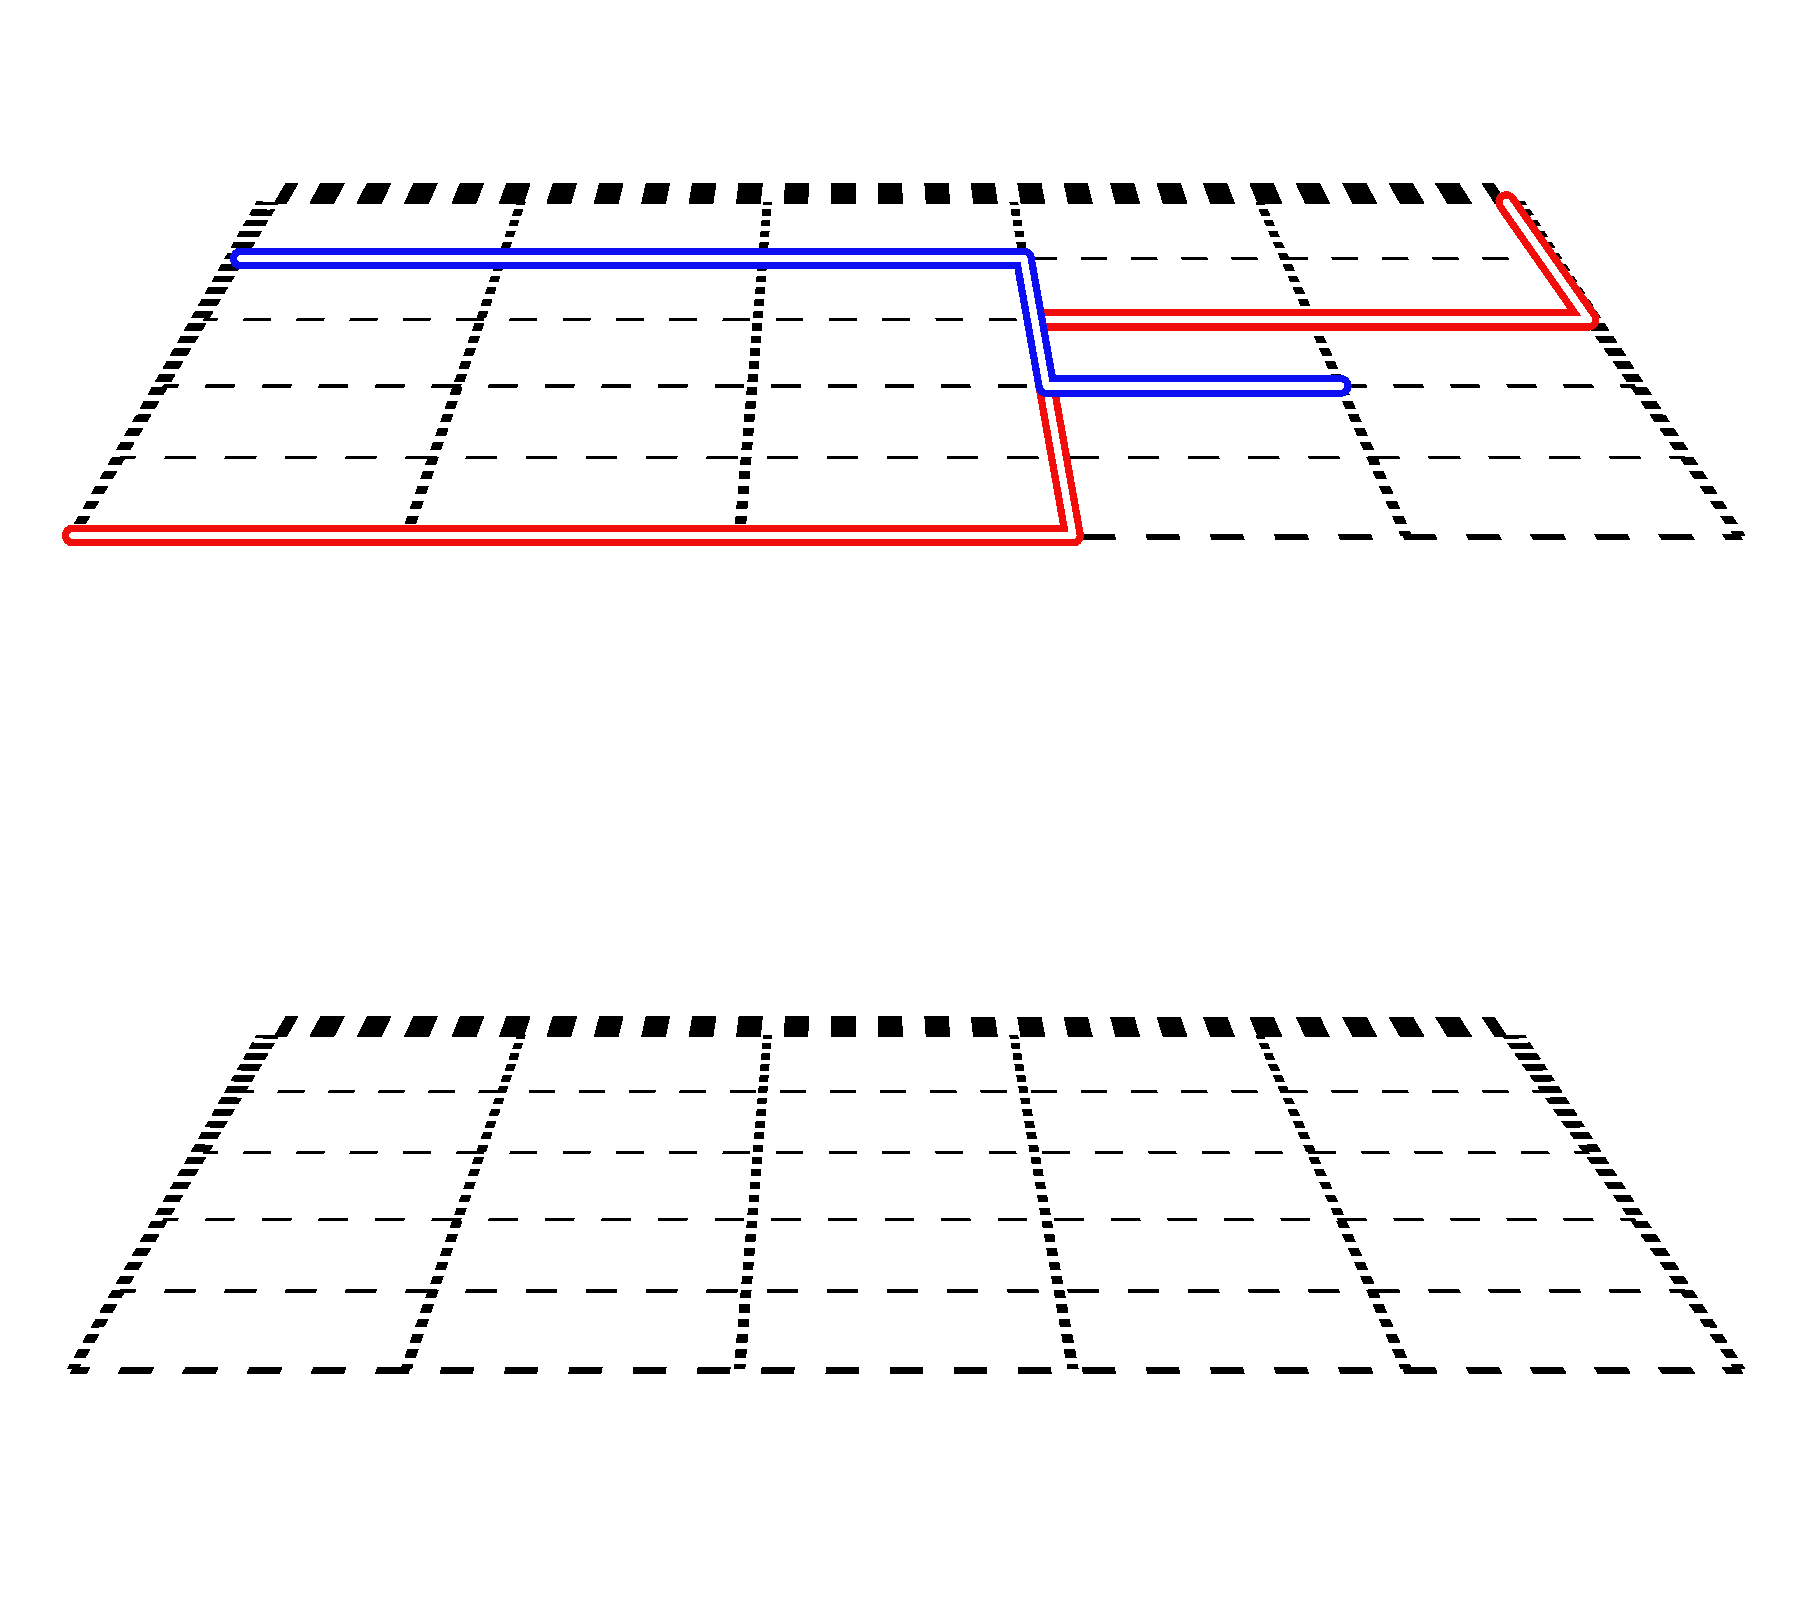
\includegraphics[width=0.8\textwidth]{deux_layers_0.pdf}
        \caption{The two layers}
        \label{fig:2layer_0}
    \end{subfigure}%
    \begin{subfigure}{0.33\textwidth}
        \centering
        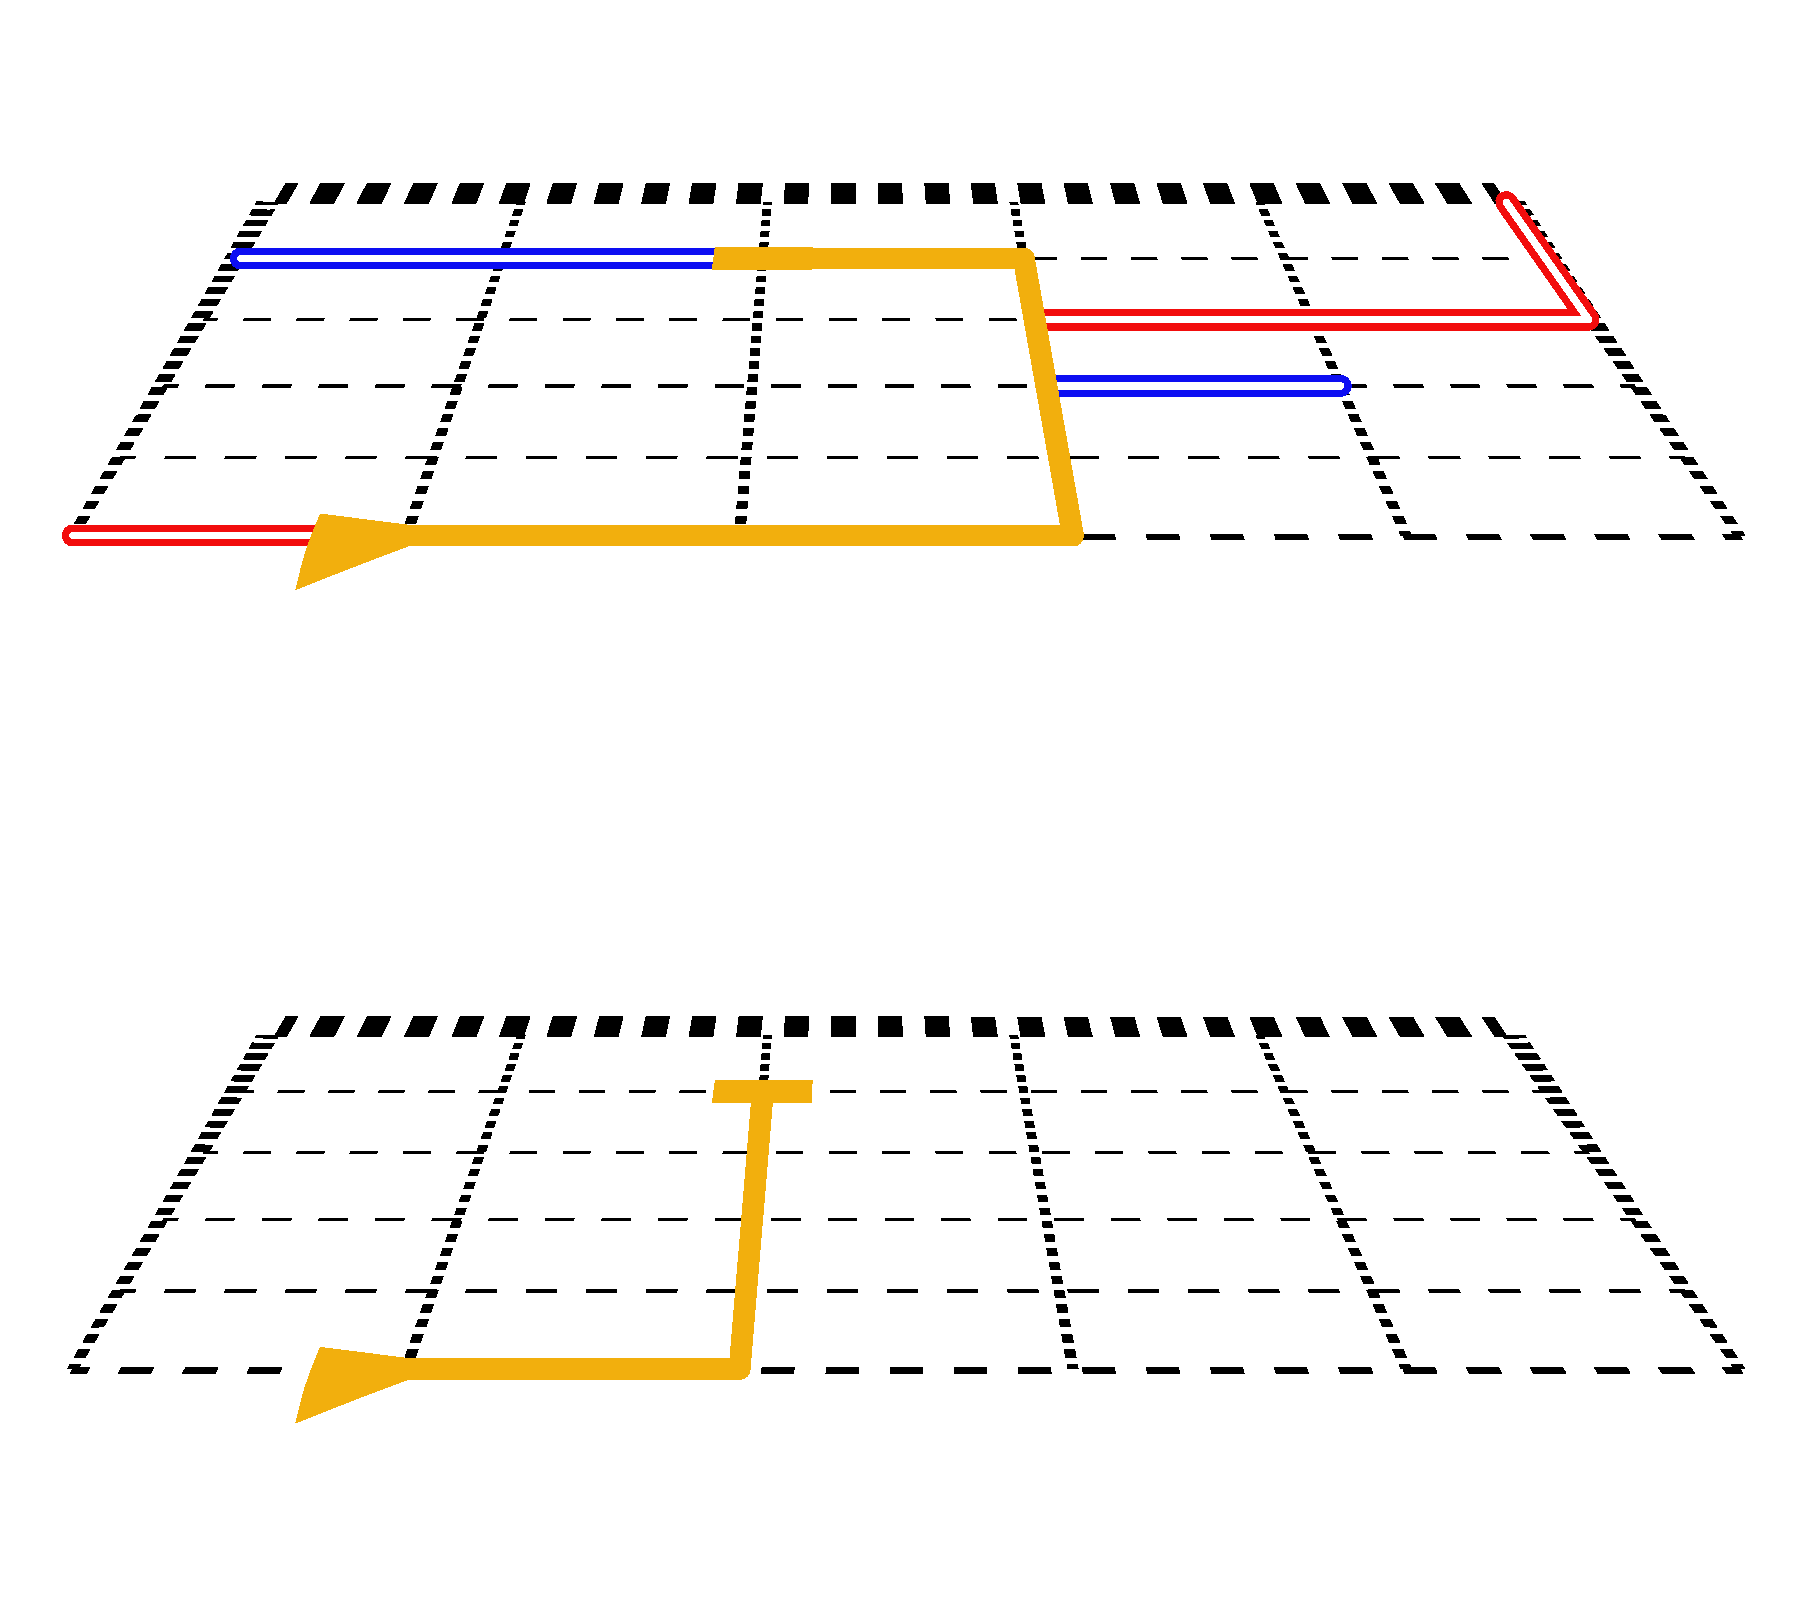
\includegraphics[width=0.8\textwidth]{deux_layers_1.pdf}
        \caption{A path on each layer}
        \label{fig:2layer_1}
    \end{subfigure}
    \begin{subfigure}{0.33\textwidth}
        \centering
        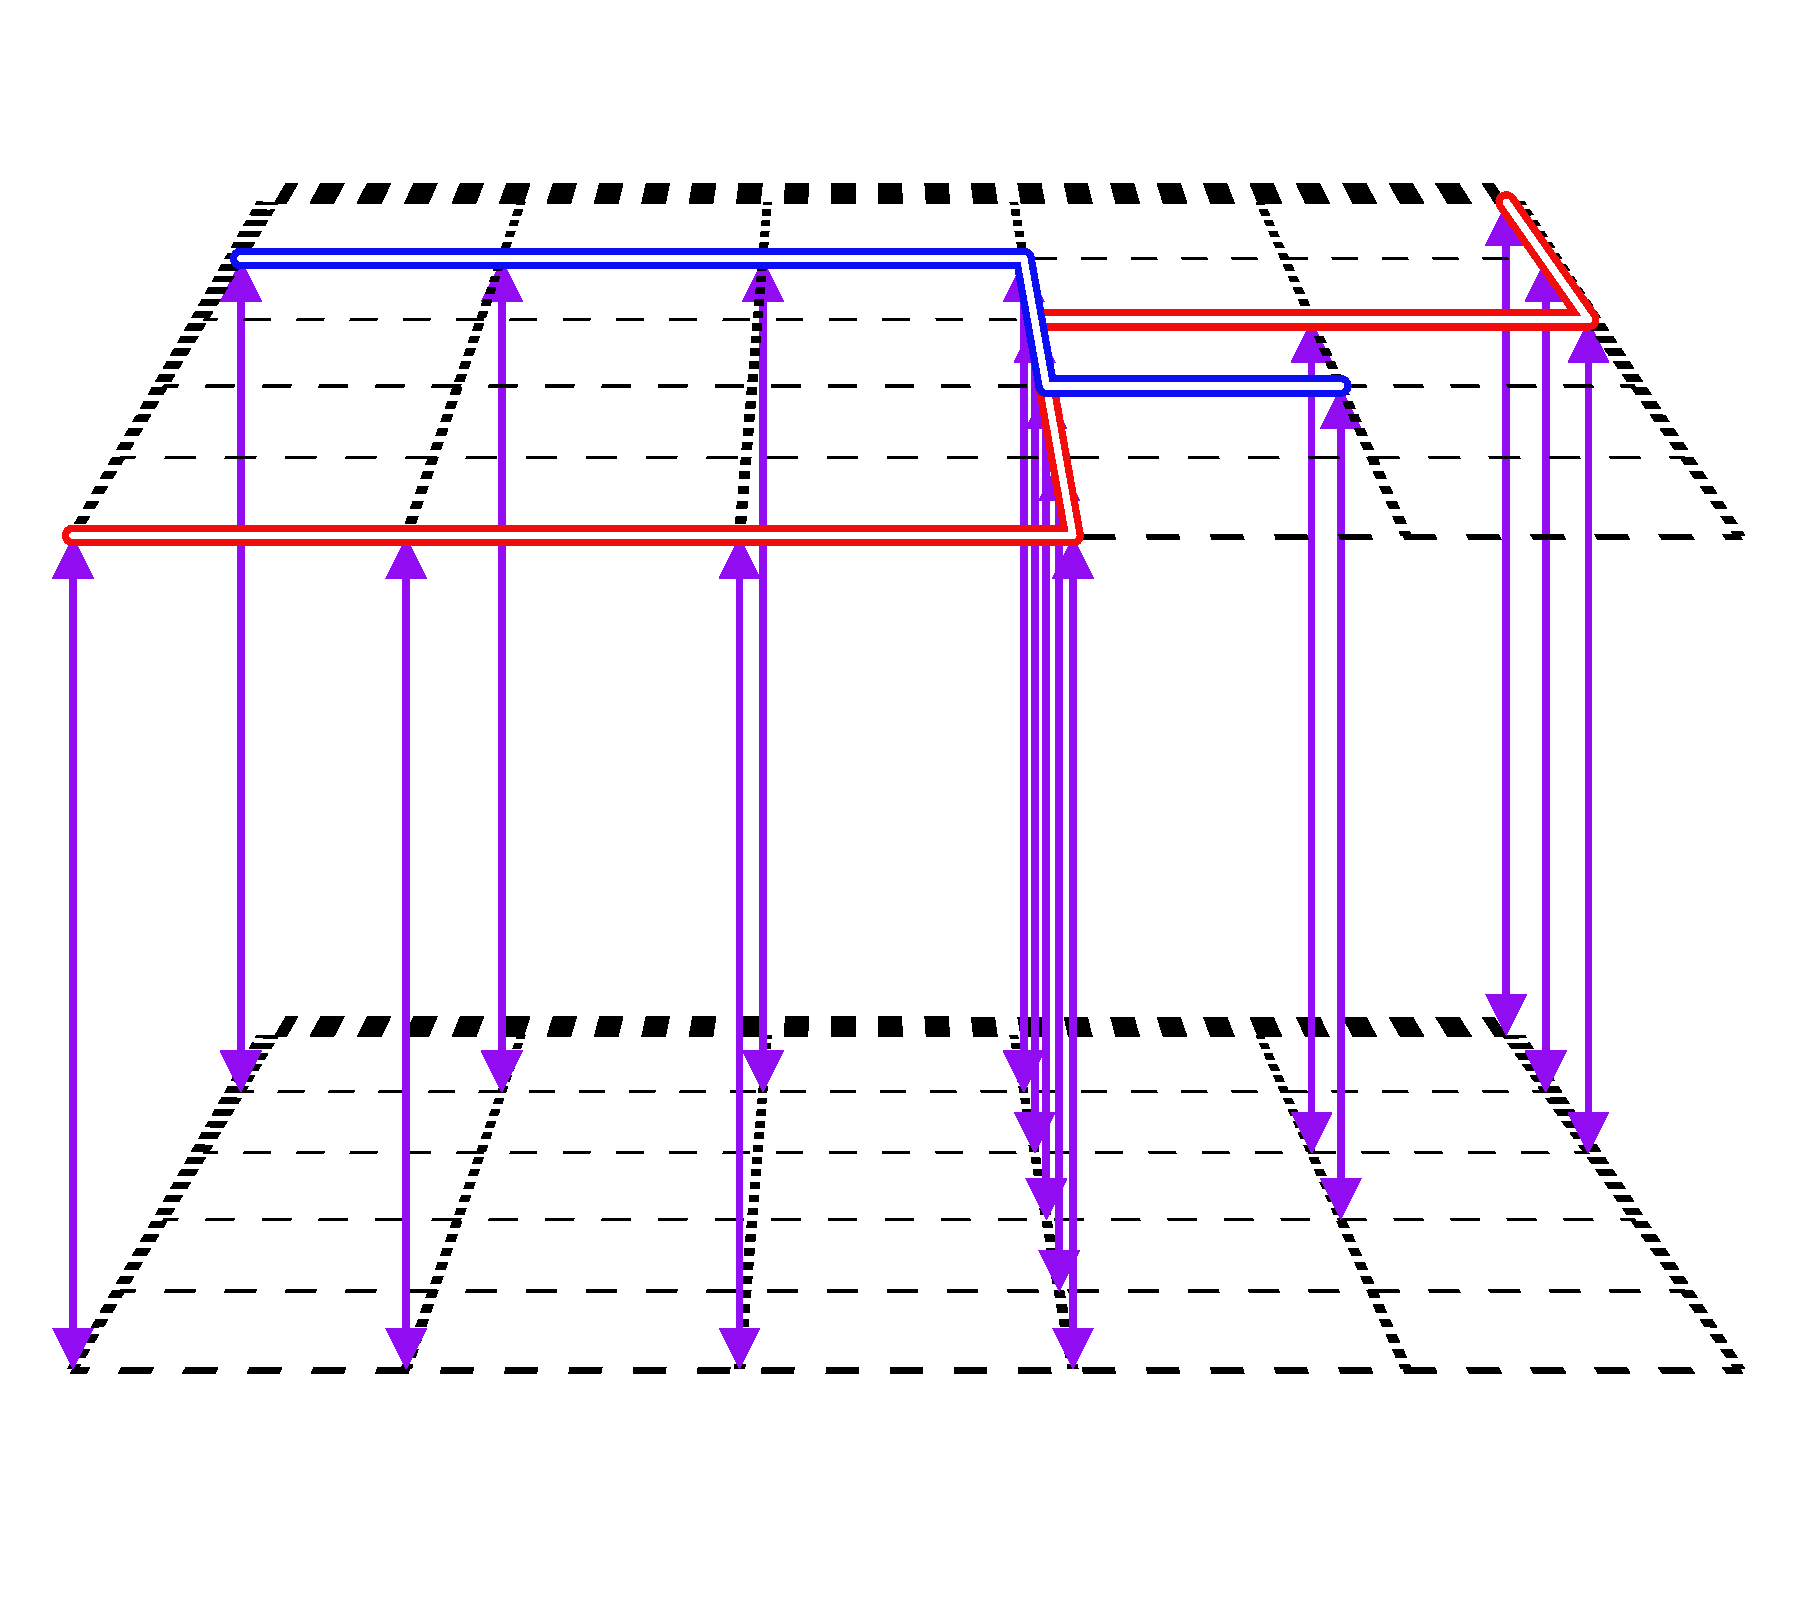
\includegraphics[width=0.8\textwidth]{deux_layers_2.pdf}
        \caption{Adding connections\\}
        \label{fig:2layer_2}
    \end{subfigure}%
    \begin{subfigure}{0.33\textwidth}
        \centering
        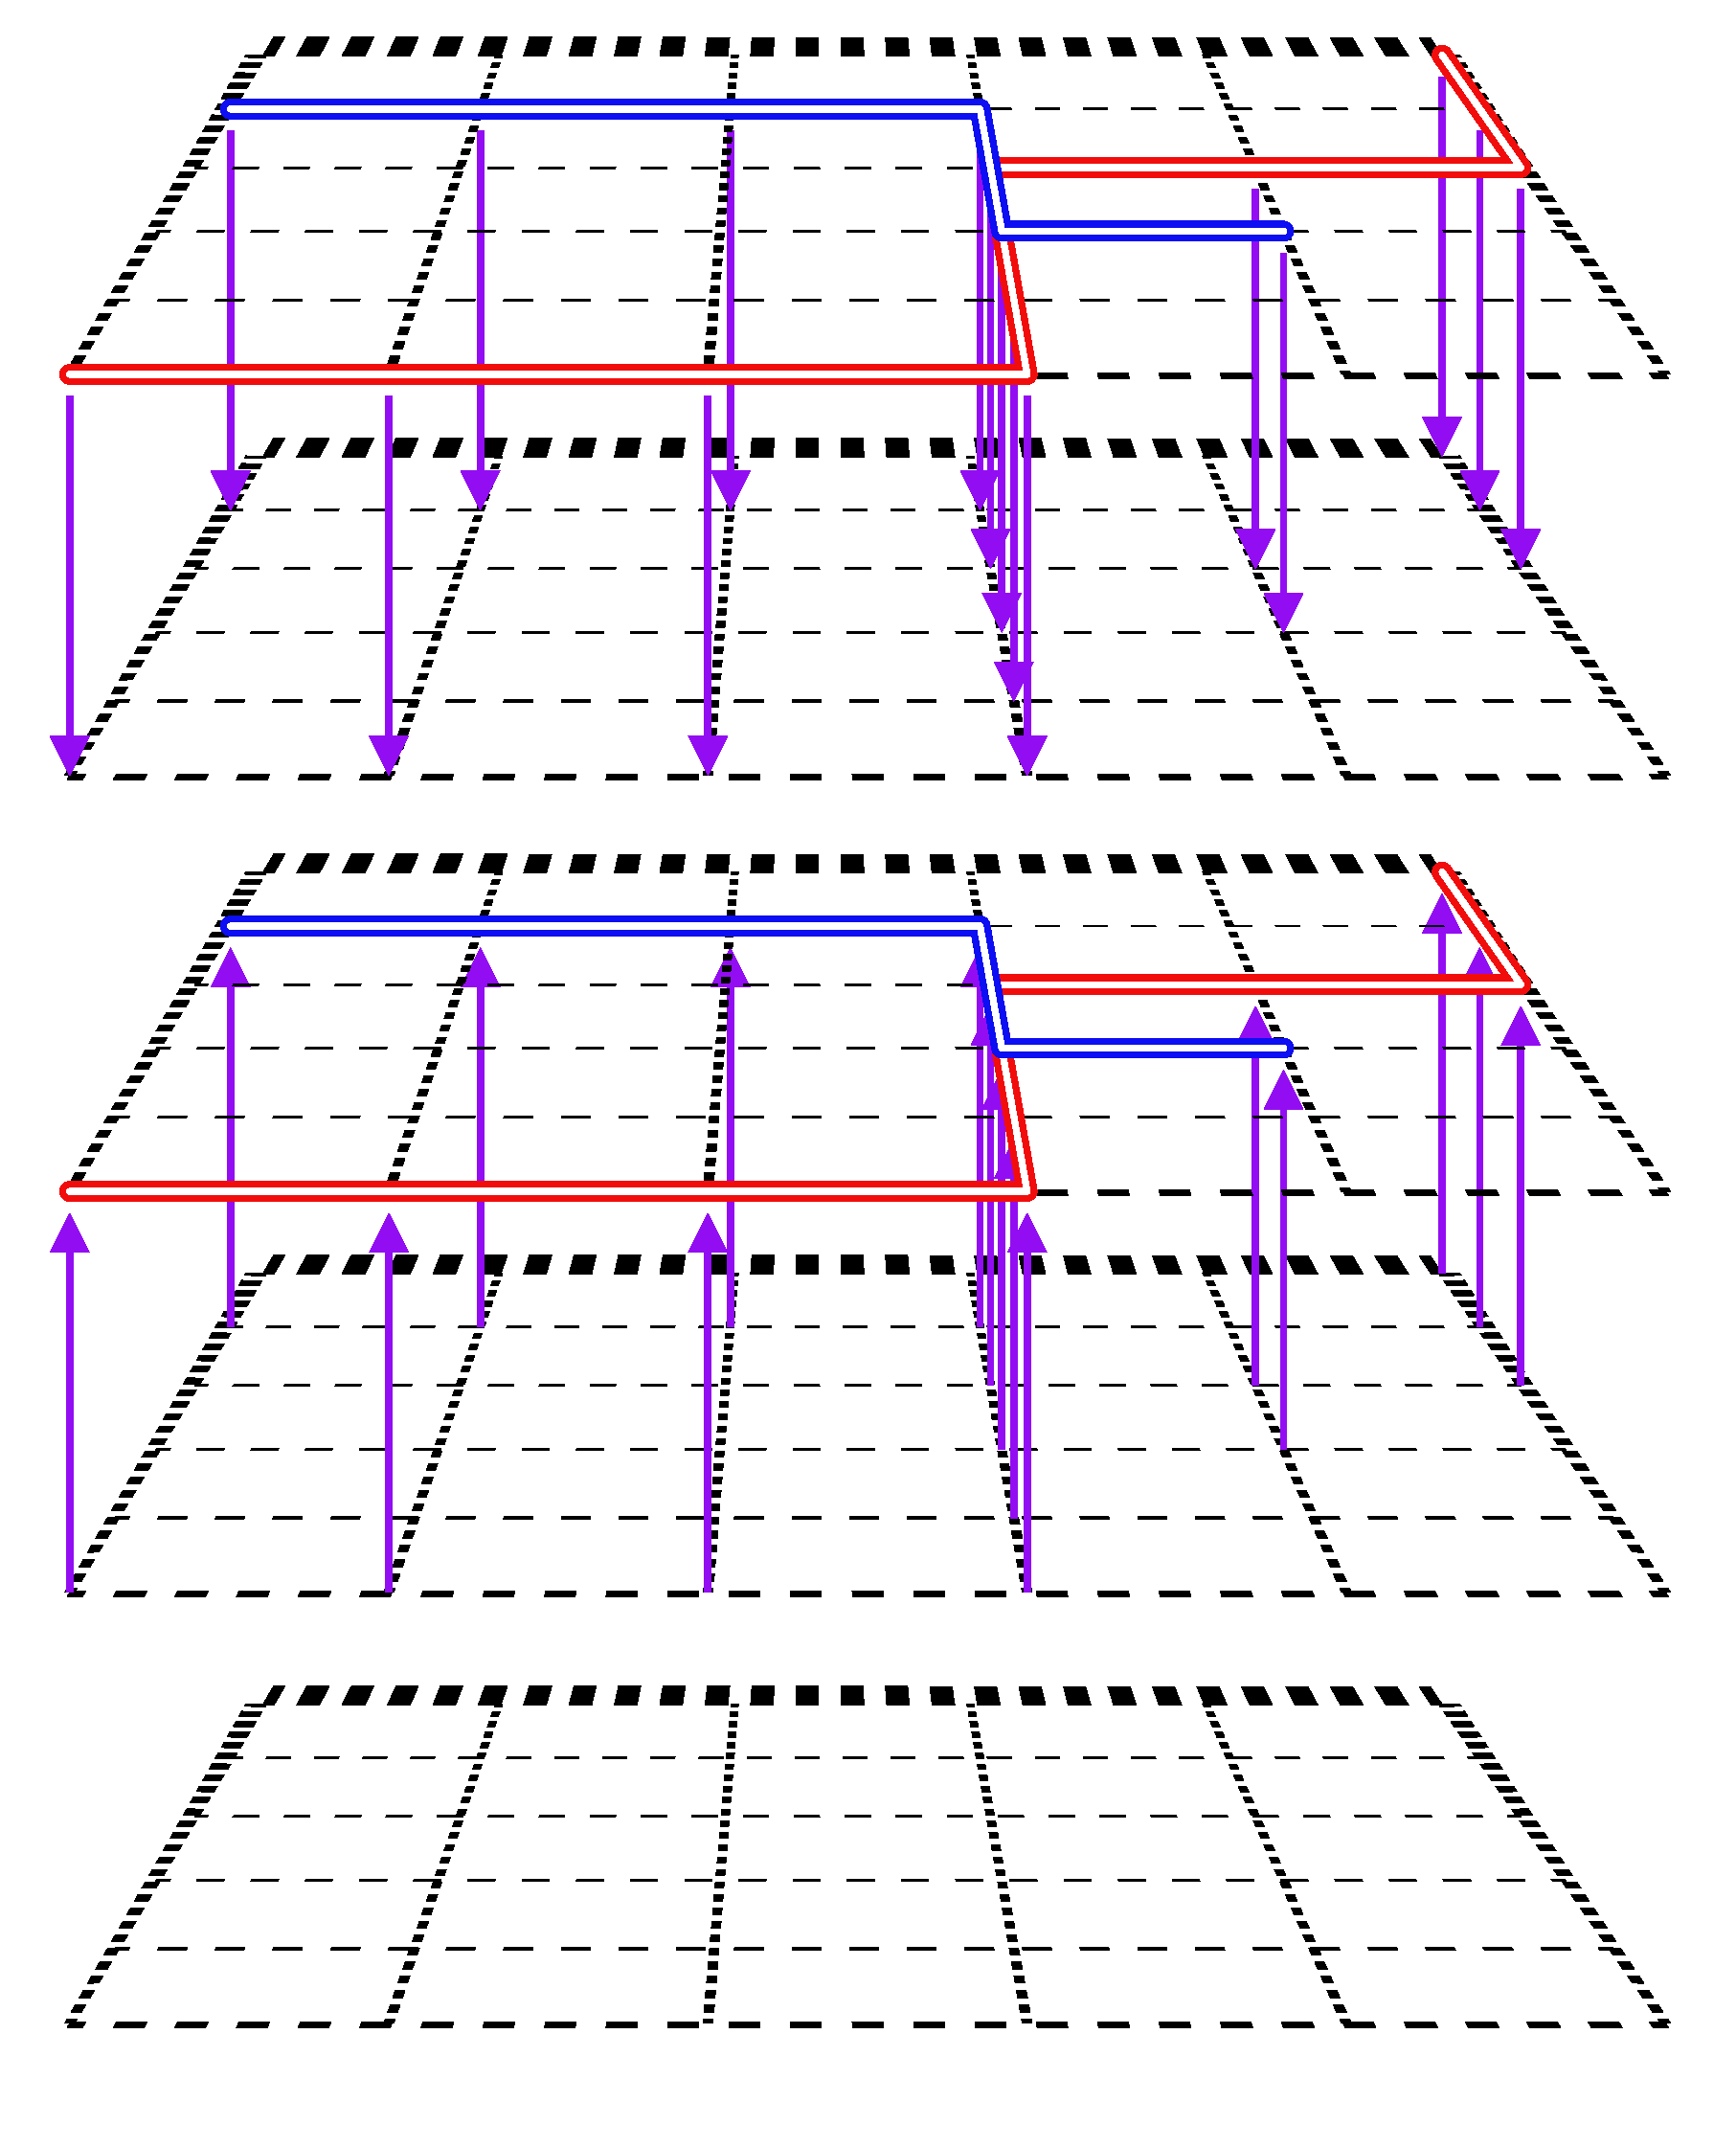
\includegraphics[width=0.6\textwidth]{deux_layers_3.pdf}
        \caption{Three graphs: onboarding, offboarding, and road only}
        \label{fig:2layer_3}
    \end{subfigure}%
    \begin{subfigure}{0.33\textwidth}
        \centering
        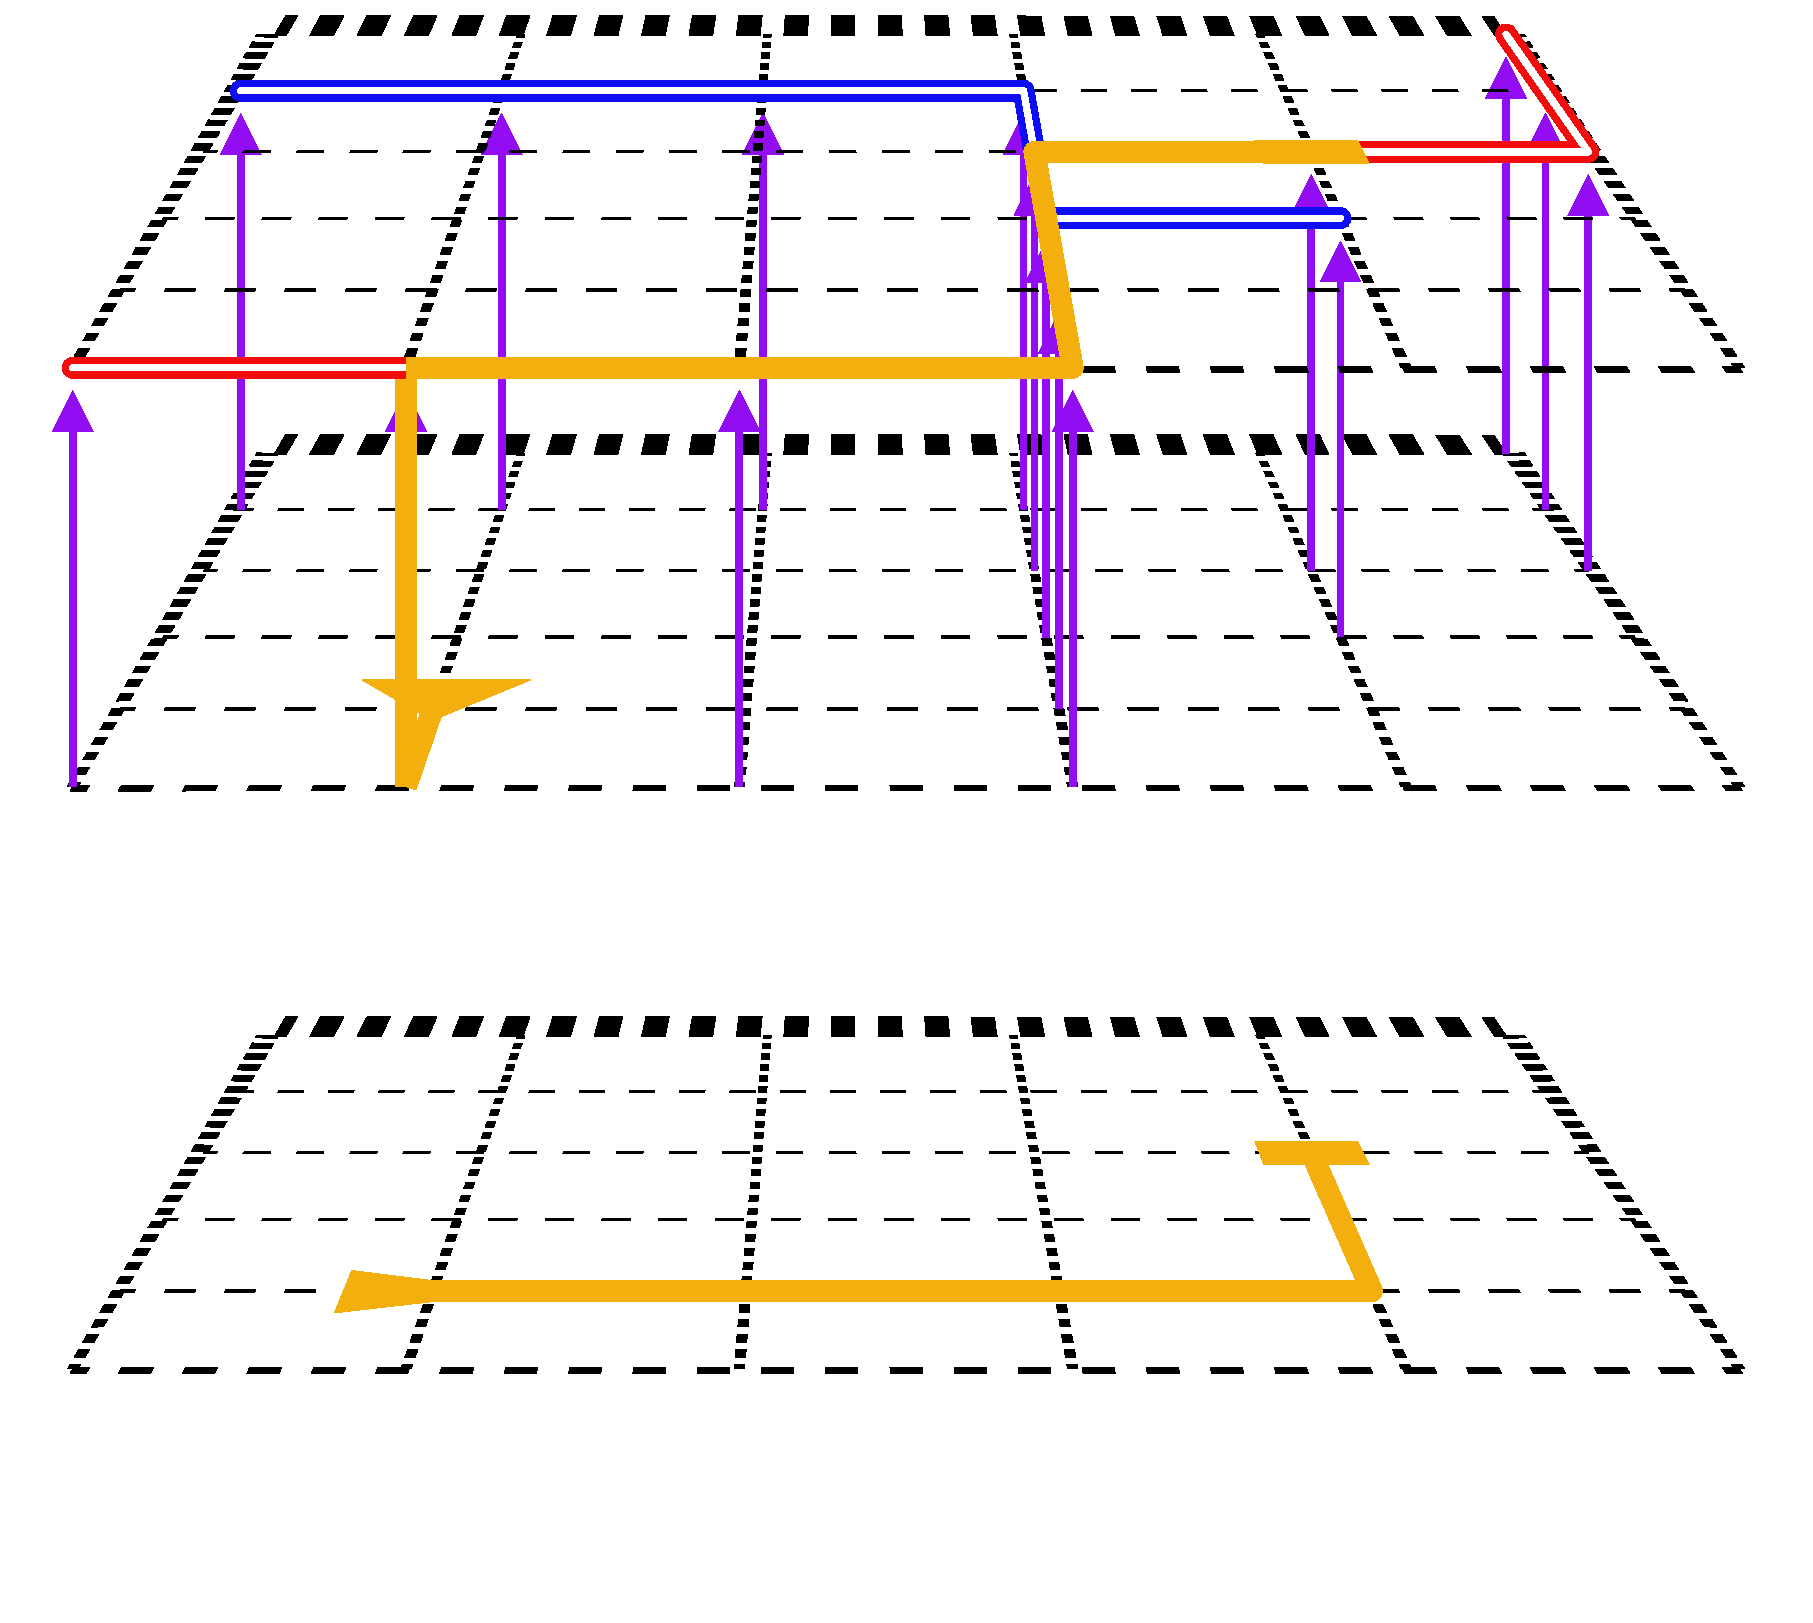
\includegraphics[width=0.8\textwidth]{deux_layers_4.pdf}
        \caption{A path on the onboarding and road networks}
        \label{fig:2layer_4}
    \end{subfigure}%
    \caption{Two-layer network}
\end{figure}

In scenario \textbf{3. P\&R}, we add zero-cost connection links between the two layers at stations (Figure \ref{fig:2layer_2}). However, travelers cannot use the tram network in the middle of their trip (see the assumptions). For each all-or-nothing assignment, we consider three graphs (Figure \ref{fig:2layer_3}) :
\begin{enumerate}
    \item \textbf{Onboarding graph:} Two layers, with links only from the road layer to the tram layer. For OD pairs where the destination is served by a tram station, we compute the shortest path from the origin node on the road layer to the destination node on the tram layer.
    \item \textbf{Offboarding graph:} Two layers, with links only from the tram layer to the road layer. For OD pairs where the origin is served by a tram station, we compute the shortest path from the origin node on the tram layer to the destination node on the road layer.
    \item \textbf{Road graph:} Road network only. We compute the shortest path for all OD pairs.
\end{enumerate}

Depending on the origin-destination pair, we may have computed three different shortest paths. We assign the traffic according to the shortest travel time.


